\documentclass[11pt,reqno]{amsbook}

 %\usepackage{makeidx}
 \usepackage{amssymb}
 \usepackage{amscd}
 %\usepackage{amsthm}
 \usepackage{graphics}
 \usepackage[all]{xy}
 %\usepackage{showkeys}
 \usepackage[plainpages=false,pagebackref=true,hypertex]{hyperref}
     %plainpages=false corrects page numbers in index
     %pagebackref=true [provides back references from bibliography]




\makeindex

 \setlength{\textwidth}{6.5in}
 \setlength{\oddsidemargin}{0in}
 \setlength{\evensidemargin}{0in}
 \setlength{\textheight}{9.25in}
 \setlength{\topmargin}{-0.35in}



\input diagxy


\allowdisplaybreaks[1]

\swapnumbers
\theoremstyle{plain}
\newtheorem{thm}{Theorem}[section]
\newtheorem{lem}[thm]{Lemma}
\newtheorem{prop}[thm]{Proposition}
\newtheorem{cor}[thm]{Corollary}
\newtheorem{ax}[thm]{Axiom}


\theoremstyle{definition}
\newtheorem{defn}[thm]{Definition}
\newtheorem{notn}[thm]{Notation}
\newtheorem{conv}[thm]{Convention}


\theoremstyle{remark}
\newtheorem*{rem}{Remark}
\newtheorem*{cau}{CAUTION}
\newtheorem{fact}[thm]{Fact}
\newtheorem{exam}[thm]{Example}
\newtheorem{exer}[thm]{Exercise}
\newtheorem{prob}[thm]{Problem}
%\newtheorem{proj}[thm]{Project}
\newtheorem{prf}[thm]{}


\renewcommand{\thechapter}{\arabic{chapter}}
\renewcommand{\thesection}{\thechapter.\arabic{section}}
\renewcommand{\thesubsection}{\thesection.\arabic{subsection}}

\renewcommand{\arraystretch}{1.5}



\numberwithin{equation}{chapter}

 \newcommand{\field}[1]{\mathbb{#1}}
 \newcommand{\C}{\field{C}}
 \newcommand{\E}{\field{E}}
 \newcommand{\N}{\field{N}}
 \newcommand{\Po}{\field{P}}
 \newcommand{\Q}{\field{Q}}
 \newcommand{\R}{\field{R}}
 \newcommand{\Sp}{\field{S}}
 \newcommand{\Z}{\field{Z}}



 \newcommand{\sto}{\rightarrow}
      %Diagxy redefined \to . This shortens the arrow.
 \newcommand{\ofml}[1]{\mathfrak{#1}}
      % for families of operators
 \newcommand{\fml}[1]{\mathcal{#1}}
      % for families of functions
 \newcommand{\sfml}[1]{\mathfrak{#1}}
      % for families of sets
 \newcommand{\df}[1]{\textsc{#1}}
      % for terms being defined
 \newcommand{\lobo}[1]{\mathfrak{#1}}
      % big oh and little oh functions
 \newcommand{\D}{\displaystyle}
 \newcommand{\ns}{\renewcommand{\qed}{}}
       % deletes end-of-proof sign
 \newcommand{\abs}[1]{\lvert#1\rvert}
       % absolute value
 \newcommand{\bigabs}[1]{\left\lvert#1\right\rvert}
       % large absolute value
 \newcommand{\norm}[1]{\lVert#1\rVert}
       % norm
 \newcommand{\bignorm}[1]{\left\lVert#1\right\rVert}
       % large norm
 \newcommand{\trinorm}[1]{\vert\mspace{-2mu}\vert
     \mspace{-2mu}\vert#1\vert\mspace{-2mu}\vert
     \mspace{-2mu}\vert}
       % 3-bar norm
 \newcommand{\id}[1]{\operatorname{id_{#1}}}
       % Identity on #1
 \newcommand{\intr}[1]{#1^{\circ}}
       % interior
 \newcommand{\clo}[1]{\overline{#1}}
       % closure
 \newcommand{\conj}[1]{\overline{#1}}
       % complex conjugate
 \newcommand{\open}[2]{#1\overset{\thickspace{}_\circ}{\subseteq}#2}
       % #1 is an open subset of #2
 \newcommand{\pd}[2]{\frac{\partial#1}{\partial#2}}
       % partial derivative of #1 wrt #2
 \newcommand{\cpd}[3]{\left(\frac{\partial#1}{\partial#2}\right)_{#3}}
       % partial derivative of #1 wrt #2 with #3 held constant
 \newcommand{\dt}[2]{d^{\,2}\!#1_{#2}}
       % 2nd differential of #1 at #2
 \newcommand{\delt}[2]{\Delta^2\!#1_{#2}}
       % 2nd difference of #1 at #2
 \newcommand{\simt}[2]{#1\overset{\scriptscriptstyle2}{\simeq}#2}
       % 2nd order tangency
 \newcommand{\locinv}[1]{#1_{\mathstrut\text{loc}}^{\mathstrut{-1}}}
       % local inverse
 \newcommand{\sbsb}[2]{#1_{{}_\sst{#2}}}
      % makes smaller, lower subscript
 \newcommand{\sst}[1]{{\scriptstyle{#1}}}
       % sub- and superscript size type
 \newcommand{\ssst}[1]{{\scriptscriptstyle{#1}}}
       % second level sub- and superscripts
 \newcommand{\symdif}[2]{#1 \bigtriangleup #2}
       % symmetric difference
 \newcommand{\vc}[1]{\mathbf{#1}}
      % for vectors
 \newcommand{\wh}[1]{\widehat{#1}}
 \newcommand{\wt}[1]{\widetilde{#1}}



 \DeclareMathOperator{\card}{card}
 \DeclareMathOperator{\diam}{diam}
 \DeclareMathOperator{\dom}{dom}
 \DeclareMathOperator{\inv}{Inv}
 \DeclareMathOperator{\ran}{ran}


\font\fiverm=cmr5



\begin{document}
\frontmatter
\title{A ProblemText in Advanced Calculus}
\author{John M. Erdman\\
     Portland State University \\
     \mbox{\hphantom{P}} \\
     Version July 1, 2014}
\date{2014}



\maketitle

\tableofcontents

\chapter*{PREFACE}

In American universities two distinct types of courses are often called ``Advanced
Calculus'': one, largely for engineers, emphasizes advanced computational techniques in
calculus; the other, a more ``theoretical'' course, usually taken by majors in
mathematics and physical sciences (and often called \emph{elementary analysis} or
\emph{intermediate analysis}), concentrates on conceptual development and proofs. This
\emph{ProblemText} is a book of the latter type. It is not a place to look for
post-calculus material on Fourier series, Laplace transforms, and the like.  It is
intended for students of mathematics and others who have completed (or nearly completed)
a standard introductory calculus sequence and who wish to understand where all those
rules and formulas come from.

Many advanced calculus texts contain more topics than this \emph{ProblemText}.  When
students are encouraged to develop much of the subject matter for themselves, it is not
possible to ``cover'' material at the same breathtaking pace that can be achieved by a
truly determined lecturer. But, while no attempt has been made to make the book
encyclopedic, I do think it nevertheless provides an integrated overview of Calculus and,
for those who continue, a solid foundation for a first year graduate course in Real
Analysis.


As the title of the present document, \emph{ProblemText in Advanced Calculus}, is
intended to suggest, it is as much an extended problem set as a textbook.  The proofs of
most of the major results are either \emph{exercises} or \emph{problems}.  The
distinction here is that solutions to \emph{exercises} are written out in a separate
chapter in the ProblemText while solutions to \emph{problems} are not given.  I hope that
this arrangement will provide flexibility for instructors who wish to use it as a text.
For those who prefer a (modified) Moore-style development, where students work out and
present most of the material, there is a quite large collection of problems for them to
hone their skills on.  For instructors who prefer a lecture format, it should be easy to
base a coherent series of lectures on the presentation of solutions to thoughtfully
chosen problems.

I have tried to make the \emph{ProblemText} (in a rather highly qualified sense discussed
below) ``self-contained''. In it we investigate how the edifice of calculus can be
grounded in a carefully developed substrata of sets, logic, and numbers.  Will it be a
``complete'' or ``totally rigorous'' development of the subject? Absolutely not.  I am
not aware of any serious enthusiasm among mathematicians I know for requiring rigorous
courses in \emph{Mathematical Logic} and \emph{Axiomatic Set Theory} as prerequisites for
a first introduction to analysis.  In the use of the tools from set theory and formal
logic there are many topics that because of their complexity and depth are cheated, or
not even mentioned. (For example, though used often, the \emph{axiom of choice} is
mentioned only once.) Even everyday topics such as ``arithmetic,'' see
appendix~\ref{arithmetic}, are not developed in any great detail.

Before embarking on the main ideas of Calculus proper one \emph{ideally} should have a
good background in all sorts of things: quantifiers, logical connectives, set operations,
writing proofs, the arithmetic and order properties of the real numbers, mathematical
induction, least upper bounds, functions, composition of functions, images and inverse
images of sets under functions, finite and infinite sets, countable and uncountable sets.
On the one hand all these are technically prerequisite to a careful discussion of the
foundations of calculus. On the other hand any attempt to do all this business
systematically at the beginning of a course will defer the discussion of anything
concerning calculus proper to the middle of the academic year and may very well both bore
and discourage students.  Furthermore, in many schools there may be students who have
already studied much of this material (in a ``proofs'' course, for example). In a spirit
of compromise and flexibility I have relegated this material to appendices. Treat it any
way you like.  I teach in a large university where students show up for Advanced Calculus
with a wide variety of backgrounds, so it is my practice to go over the appendices first,
covering many of them in a quite rapid and casual way, my goal being to provide just
enough detail so that everyone will know where to find the relevant material when they
need it later in the course.  After a rapid traversal of the appendices I start
Chapter~$1$.

For this text to be useful a student should have previously studied introductory
calculus, more for mathematical maturity than anything else.  Familiarity with properties
of elementary functions and techniques of differentiation and integration may be assumed
and made use of in \emph{examples}---but is never relied upon in the logical development
of the material.

One motive for my writing this text is to make available in fairly simple form material
that I think of as ``calculus done right.''  For example, differential calculus as it
appears in many texts is a morass of tedious epsilon-delta arguments and partial
derivatives, the net effect of which is to almost totally obscure the beauty and elegance
which results from a careful and patient elaboration of the concept of tangency. On the
other hand texts in which things are done right (for example Loomis and
Sternberg~\cite{LoomisS:1990}) tend to be rather forbidding.  I have tried to write a
text which will be helpful to a determined student with an average background.  (I
seriously doubt that it will be of much use to the chronically lazy or totally
unengaged.)

In my mind one aspect of doing calculus ``correctly'' is arrange things so that there is
nothing to unlearn later.  For example, in this text topological properties of the real
line are discussed early on.  Later, topological things (continuity, compactness,
connectedness, and so on) are discussed in the context of metric spaces (because they
unify the material conceptually and greatly simplify subsequent arguments).  But the
important thing is the \emph{definitions} in the single variable case and the metric
space case are the same. Students do not have to ``unlearn'' material as they go to more
general settings.  Similarly, the differential calculus is eventually developed in its
natural habitat of normed linear spaces.  But here again, the student who has mastered
the one-dimensional case, which occurs earlier in the text, will encounter definitions
and theorems and proofs that are virtually identical to the ones with which (s)he is
already familiar.  There is nothing to unlearn.

In the process of writing this \emph{ProblemText} I have rethought the proofs of many
standard theorems. Although some, perhaps most, results in advanced calculus have reached
a final, optimal form, there are many others that, despite dozens of different approaches
over the years, have proofs that are genuinely confusing to most students.  To mention
just one example there is the theorem concerning change of order of differentiation whose
conclusion is
  \[ \frac{\partial^2f}{\partial x \, \partial y} =
               \frac{\partial^2f}{\partial y \, \partial x}\,. \]
This well-known result to this day still receives clumsy, impenetrable, and even
incorrect proofs. I make an attempt, here and elsewhere in the text, to lead students to
proofs that are conceptually clear, even when they may not be the shortest or most
elegant.  And throughout I try very hard to show that mathematics is about ideas and not
about manipulation of symbols.

There are of course a number of advantages and disadvantages in consigning a document to
electronic life. One slight advantage is the rapidity with which links implement
cross-references.  Hunting about in a book for \emph{lemma 3.14.23} can be time-consuming
(especially when an author engages in the entirely logical but utterly infuriating
practice of numbering lemmas, propositions, theorems, corollaries, \emph{etc.}
separately).  A perhaps more substantial advantage is the ability to correct errors, add
missing bits, clarify opaque arguments, and remedy infelicities of style in a timely
fashion.  The correlative disadvantage is that a reader returning to the web page after a
short time may find everything (pages, definitions, theorems, sections) numbered
differently.  (\LaTeX is an amazing tool.) I will change the date on the title page to
inform the reader of the date of the last nontrivial update (that is, one that affects
numbers or cross-references).

The most serious disadvantage of electronic life is impermanence.  In most cases when a
web page vanishes so, for all practical purposes, does the information it contains.  For
this reason (and the fact that I want this material to be freely available to anyone who
wants it) I am making use of a ``Share Alike'' license from Creative Commons. It is my
hope that anyone who finds this text useful will correct what is wrong, add what is
missing, and improve what is clumsy.  To make this possible I am also including the
\LaTeX source code on my web page. For more information on creative commons licenses see
   \[ \text{http://creativecommons.org/} \]

I extend my gratitude to the many students over the years who have endured various
versions of this ProblemText and to my colleagues who have generously nudged me when they
found me napping.  I want especially to thank Dan Streeter who provided me with so much
help in the technical aspects of getting this document produced.  The text was prepared
using \AmS-\LaTeX. For the diagrams I used the macro package \Xy-pic by Kristoffer H.
Rose and Ross Moore supplemented by additional macros in the diagxy package by Michael
Barr.

Finally it remains only to say that I will be delighted to receive, and will consider,
any comments, suggestions, or error reports. My e-mail address is
  \[  \text{erdman@pdx.edu} \]


 \cleardoublepage
 \phantomsection
        %allows TOC links to find preface correctly


\include{htu}


\mainmatter

 \chapter{INTERVALS}\label{intervals}

The three great realms of calculus are differential calculus, integral calculus, and the
theory of infinite series.  Central to each of these is the notion of \emph{limit}:
derivatives, integrals, and infinite series can be defined as limits of appropriate objects.
Before entering these realms, however, one must have some background.  There are the basic
facts about the algebra, the order properties, and the topology of the real line~$\R$.  One
must know about functions and the various ways in which they can be combined (addition,
composition, and so on). And, finally, one needs some basic facts about continuous functions,
in particular the \emph{intermediate value theorem} and the \emph{extreme value theorem}.

%As was mentioned in the section \emph{How to Use This Book}, much
Much of this material appears in the appendices.  The remainder (the topology of $\R$,
continuity, and the \emph{intermediate} and \emph{extreme value theorems}) occupies the first
six chapters. After these have been completed we proceed with limits and the differential
calculus of functions of a single variable.

As you will recall from beginning calculus we are accustomed to calling certain intervals
``open'' (for example, $(0,1)$ and $(-\infty, 3)$ are open intervals) and other intervals
``closed'' (for example, $[0,1]$ and $[1,\infty)$ are closed intervals).  In this chapter and
the next we investigate the meaning of the terms ``open'' and ``closed''.  These concepts turn
out to be rather more important than one might at first expect.  It will become clear after
our discussion in subsequent chapters of such matters as continuity, connectedness, and
compactness just how important they really are.

\section{DISTANCE AND NEIGHBORHOODS}
\begin{defn} If $x$ and $a$ are real numbers, the
 \index{distance!between real numbers}%
\df{distance between} $x$ and $a$, which we denote by $d(x,a)$, is defined to be $\abs{x-a}$.
\end{defn}

\begin{exam} There are exactly two real numbers whose distance from the number $3$ is~$7$.
\end{exam}

\begin{proof} We are looking for all numbers $x \in \R$ such that $d(x,3)=7$. In other words
we want solutions to the equation $\abs{x-3}=7$.  There are two such solutions.  If $x-3 \ge
0$, then $\abs{x-3} = x-3$; so $x=10$ satisfies the equation.  On the other hand, if $x-3 <
0$, then $\abs{x-3} = -(x-3) = 3-x$, in which case $x=-4$ is a solution.
\end{proof}


\begin{exer}\label{1exer1} Find the set of all points on the real line which are within $5$
units of the number~$-2$. (Solution~\ref{sol_1exer1}.)
\end{exer}

\begin{prob} Find the set of all real numbers whose distance from $4$ is greater than~$15$.
\end{prob}

\begin{defn} Let $a$ be a point in $\R$ and $\epsilon > 0$.  The open interval
$(a - \epsilon, a + \epsilon)$ centered at $a$ is called the
 \index{epsilon@$\epsilon$-neighborhood}%
 \index{neighborhood!of a point}%
\df{$\epsilon$-neighborhood} of $a$ and is denoted
 \index{<@$J_\epsilon(a)$ ($\epsilon$-neighborhood about~$a$)}%
 \index{j@$J_\epsilon(a)$ ($\epsilon$-neighborhood about~$a$)}%
by~$J_\epsilon(a)$.  Notice that this neighborhood consists of all
numbers $x$ whose distance from $a$ is less than $\epsilon$; that
is, such that $\abs{x-a}<\epsilon$.
\end{defn}

\begin{exam} The $\frac12$\,-\,neighborhood of $3$ is the open interval
$\bigl(\frac52,\frac72\bigr)$.
\end{exam}

\begin{proof} We have $d(x,3) < \frac12$ only if $\abs{x-3} < \frac12$.  Solve this
inequality to obtain $J_\frac12(3) = \bigl(\frac52,\frac72\bigr)$.
\end{proof}

\begin{exam} The open interval $(1,4)$ is an $\epsilon$-neighborhood of an appropriate point.
\end{exam}

\begin{proof} The midpoint of $(1,4)$ is the point $\frac52$.  The distance from this point to
either end of the interval is $\frac32$. Thus $(1,4) = J_\frac32\bigl(\frac52\bigr)$.
\end{proof}

\begin{prob} Find, if possible, a number $\epsilon$ such that the $\epsilon$-neigh\-bor\-hood
of $\frac13$ contains both $\frac14$ and $\frac12$ but does not contain $\frac{17}{30}$.
If such a neighborhood does not exist, explain why.
\end{prob}

\begin{prob} Find, if possible, a number $\epsilon$ such that the $\epsilon$-neigh\-bor\-hood
of $\frac13$ contains $\frac{11}{12}$ but does not contain either $\frac12$ or $\frac58$.  If
such a neighborhood does not exist, explain why.
\end{prob}

\begin{prob} Let $U = \bigl(\frac14, \frac23\bigr)$ and $V = \bigl(\frac12,\frac65\bigr)$.
Write $U$ and $V$ as $\epsilon$-neighborhoods of appropriate points. (That is, find
numbers $a$ and $\epsilon$ such that $U = J_\epsilon(a)$ and find numbers $b$ and
$\delta$ such that $V = J_\delta(b)$.\,)  Also write the sets $U \cup V$ and $U \cap V$
as $\epsilon$-neighborhoods of appropriate points.
\end{prob}

\begin{prob} Generalize your solution to the preceding problem to show that the union and the
intersection of any two $\epsilon$-neighborhoods which overlap is itself an
$\epsilon$-neighborhood of some point.  \emph{Hint.} Since $\epsilon$-neighborhoods are open
intervals of finite length, we can write the given neighborhoods as $(a,b)$ and $(c,d)$.
There are really just two distinct cases.  One neighborhood may contain the other; say, $a \le
c < d \le b$.  Or each may have points that are not in the other; say $a < c < b < d$.  Deal
with the two cases separately.
\end{prob}

\begin{prop}\label{d_less_e} If $a \in \R$ and $0 < \delta \le \epsilon$, then $J_\delta(a)
\subseteq J_\epsilon(a)$.
\end{prop}

\begin{proof} Exercise. (Solution~\ref{sol_d_less_e}.)
 \ns \end{proof}










\section{INTERIOR OF A SET}
\begin{defn} Let $A \subseteq \R$. A point $a$ is an
 \index{interior!point}%
\df{interior point} of $A$ if some $\epsilon$-neighborhood of $a$ lies entirely in~$A$.  That
is, $a$ is an interior point of $A$ if and only if there exists $\epsilon > 0$ such that
$J_\epsilon(a) \subseteq A$. The set of all interior points of $A$ is denoted by $A^\circ$ and
is called the
 \index{<@$A^\circ$ (interior of~$A$)}%
 \index{interior}%
\df{interior} of~$A$.
\end{defn}

\begin{exam} Every point of the interval $(0,1)$ is an interior point of that interval.  Thus
$(0,1)^\circ = (0,1)$.
\end{exam}

\begin{proof} Let $a$ be an arbitrary point in $(0,1)$.  Choose $\epsilon$ to be the smaller of
the two (positive) numbers $a$ and $1-a$.  Then $J_\epsilon(a) = (a - \epsilon, a + \epsilon)
\subseteq (0,1)$ (because $\epsilon \le a$ implies $a-\epsilon \ge 0$, and $\epsilon \le 1-a$
implies $a+\epsilon \le 1$).
\end{proof}

\begin{exam}\label{interior_open_int} If $a < b$, then every point of the interval $(a,b)$ is an
interior point of the interval.  Thus $(a,b)^\circ = (a,b)$.
\end{exam}

\begin{proof} Problem. \ns  \end{proof}

\begin{exam} The point $0$ is not an interior point of the interval~$[0,1)$.
\end{exam}

\begin{proof} Argue by contradiction.  Suppose $0$ belongs to the interior of~$[0,1)$.  Then for
some $\epsilon > 0$ the interval $(-\epsilon,\epsilon) = J_\epsilon(0)$ is contained in
$[0,1)$. But this is impossible since the number $-\frac12\epsilon$ belongs to
$(-\epsilon,\epsilon)$ but not to $[0,1)$.
\end{proof}

\begin{exam} Let $A = [a,b]$ where $a < b$.  Then $A^\circ = (a,b)$.
\end{exam}

\begin{proof} Problem. \ns \end{proof}

\begin{exam}\label{1exer3} Let $A = \{x \in \R\colon x^2-x-6 \ge 0\}$.  Then $A^\circ \ne A$.
\end{exam}

\begin{proof} Exercise. (Solution~\ref{sol_1exer3}.)
  \ns \end{proof}

\begin{prob} Let $A = \{x \in \R\colon x^3 - 2x^2 - 11x + 12 \le 0\}$.  Find $A^\circ$.
\end{prob}

\begin{exam} The interior of the set $\Q$ of rational numbers is empty.
\end{exam}

\begin{proof} No open interval contains only rational numbers.
\end{proof}

\begin{prop}\label{intr_subsets} If $A$ and $B$ are sets of real numbers with $A \subseteq B$,
then $\intr A \subseteq \intr B$.
\end{prop}

\begin{proof} Let $a \in \intr A$.  Then there is an $\epsilon > 0$ such that $J_\epsilon(a)
\subseteq A \subseteq B$.  This shows that $a \in \intr B$.
\end{proof}

\begin{prop} If $A$ is a set of real numbers, then $A^{\circ\circ} = \intr A$.
\end{prop}

\begin{proof} Problem.  \ns  \end{proof}

\begin{prop}\label{intr_intersection} If $A$ and $B$ are sets of real numbers, then
  \[\intr{(A \cap B)} = \intr A \cap \intr B.\]
\end{prop}

\begin{proof} Exercise.  \emph{Hint.}  Show separately that $\intr{(A \cap B)} \subseteq
\intr A \cap \intr B$ and that $\intr A \cap \intr B \subseteq \intr{(A \cap B)}$.
(Solution~\ref{sol_intr_intersection}.) \ns
\end{proof}

\begin{prop}\label{intr_union} If $A$ and $B$ are sets of real numbers, then
   \[ \intr{(A \cup B)} \supseteq \intr A \cup \intr B\,. \]
\end{prop}

\begin{proof} Exercise. (Solution~\ref{sol_intr_union}.) \ns \end{proof}

\begin{exam} Equality may fail in the preceding proposition.
\end{exam}

\begin{proof} Problem.  \emph{Hint.}  See if you can find sets $A$ and $B$ in $\R$ both of
which have empty interior but whose union is all of~$\R$.  \ns
\end{proof}


\endinput

 \chapter{TOPOLOGY OF THE REAL LINE}\label{nbhds_in_r}

It is clear from the definition of ``interior'' that the interior of a set is always contained
in the set.  Those sets for which the reverse inclusion also holds are called \emph{open
sets}.

\section{OPEN SUBSETS OF $\R$}
\begin{defn} A subset $U$ of $\R$ is
 \index{open}%
\df{open} if $U^\circ = U$.  That is, a set is open if and only if every point of the set is
an interior point of the set.  If $U$ is an open subset of $\R$ we
 \index{<@$\open{}{}$ (open subset of)}%
write~$\open{U}{\R}$.

Notice, in particular, that the empty set is open.  This is a consequence of the way
implication is defined in section~\ref{implication}: the condition that each point of
$\emptyset$ be an interior point is \emph{vacuously satisfied} because there \emph{are no
points} in $\emptyset$. (One argues that \emph{if} an element $x$ belongs to the empty
set, \emph{then} it is an interior point of the set.  The hypothesis is false; so the
implication is true.)  Also notice that $\R$ itself is an open subset of~$\R$.
\end{defn}

\begin{exam}\label{open_int_open} Bounded open intervals are open sets.  That is, if $a < b$,
then the open interval $(a,b)$ is an open set.
\end{exam}

\begin{proof} Example \ref{interior_open_int}. \end{proof}

\begin{exam} The interval $(0,\infty)$ is an open set.
\end{exam}

\begin{proof} Problem.  \ns \end{proof}

One way of seeing that a set is open is to verify that each of its points is an interior point
of the set.  That is what the definition says.  Often it is easier to observe that the set can
be written as a union of bounded open intervals.  That this happens exactly when a set is open
is the point of the next proposition.

\begin{prop}\label{union_open_intervals} A nonempty subset of $\R$ is open if and only if it is
a union of bounded open intervals.
\end{prop}

\begin{proof} Let $U \subseteq \R$. First, let us suppose $U$ is a nonempty open subset of~$\R$.
Each point of $U$ is then an interior point of $U$. So for each $x \in U$ we may choose a
bounded open interval $J(x)$ centered at $x$ which is entirely contained in $U$.  Since $x \in
J(x)$ for each $x \in U$, we see that
  \begin{equation}\label{2eqn1} U = \bigcup_{x \in U}\{x\} \subseteq
                \bigcup_{x \in U}J(x).
  \end{equation}
On the other hand, since $J(x) \subseteq U$ for each $x \in U$, we have (see
proposition~\ref{union_of_fam1})
  \begin{equation}\label{2eqn2} \bigcup_{x \in U} J(x) \subseteq U.
  \end{equation}
Together \eqref{2eqn1} and \eqref{2eqn2} show that $U$ is a union of bounded open intervals.

For the converse suppose $U = \bigcup \sfml{J}$ where $\sfml{J}$ is a family of open
bounded intervals.  Let $x$ be an arbitrary point of $U$.  We need only show that $x$ is
an interior point of~$U$. To this end choose an interval $J \in \sfml{J}$ which
contains~$x$. Since $J$ is a bounded open interval we may write $J = (a,b)$ where~$a <
b$.  Choose $\epsilon$ to be the smaller of the numbers $x - a$ and $b - x$.  Then it is
easy to see that $\epsilon > 0$ and that $x \in J_\epsilon(x) = (x - \epsilon, x +
\epsilon) \subseteq (a,b)$. Thus $x$ is an interior point of~$U$.
\end{proof}

\begin{exam}Every interval of the form $(-\infty,a)$ is an open set. So is every interval of
the form $(a,\infty)$. (Notice that this and example \ref{open_int_open} give us the very
comforting result that the things we are accustomed to calling open intervals are indeed open
sets.)
\end{exam}

\begin{proof} Problem. \ns \end{proof}

The study of calculus has two main ingredients: algebra and topology.  Algebra deals with
operations and their properties, and with the resulting structure of groups, fields, vector
spaces, algebras, and the like.  Topology, on the other hand, is concerned with closeness,
$\epsilon$-neighborhoods, open sets, and with the associated structure of metric spaces and
various kinds of topological spaces.  Almost everything in calculus results from the interplay
between algebra and topology.

\begin{defn} The word ``topology'' has a technical meaning.  A family $\sfml{T}$ of subsets
of a set $X$ is a
 \index{topology}%
\df{topology} on $X$ if
 \begin{enumerate}
   \item $\emptyset$ and $X$ belong to $\sfml{T}$;
   \item if $\sfml{S} \subseteq \sfml{T}$ (that is, if $\sfml S$ is a
subfamily of~$\sfml T$), then $\bigcup\sfml{S} \in \sfml{T}$; and
   \item if $\sfml{S}$ is a \emph{finite} subfamily of $\sfml{T}$, then
$\bigcap\sfml{S} \in \sfml{T}$.
 \end{enumerate}
\end{defn}

We can paraphrase this definition by saying that a family of subsets of $X$, which contains
both $\emptyset$ and $X$, is a topology on $X$ if it is closed under arbitrary unions and
finite intersections.  If this definition doesn't make any sense to you at first reading,
don't fret.  This kind of abstract definition, although easy enough to remember, is
irritatingly difficult to understand.  Staring at it doesn't help. It appears that a
bewildering array of entirely different things might turn out to be topologies.  And this is
indeed the case.  An understanding and appreciation of the definition come only gradually.
You will notice as you advance through this material that many important concepts such as
continuity, compactness, and connectedness are defined by (or characterized by) open sets.
Thus theorems which involve these ideas will rely on properties of open sets for their proofs.
This is true not only in the present realm of the real line but in the much wider world of
metric spaces, which we will shortly encounter in all their fascinating variety. You will
notice that two properties of open sets are used over and over: that unions of open sets are
open and that finite intersections of open sets are open.  Nothing else about open sets turns
out to be of much importance.  Gradually one comes to see that these two facts completely
dominate the discussion of continuity, compactness, and so on.  Ultimately it becomes clear
that nearly everything in the proofs goes through in situations where \emph{only} these
properties are available---that is, in topological spaces.

Our goal at the moment is quite modest: we show that the family of all open subsets of $\R$ is
indeed a topology on $\R$.

\begin{prop}\label{union_intersection_open} Let $\sfml S$ be a family of open sets in $\R$.
Then
 \begin{enumerate}
   \item[(a)] the union of $\sfml S$ is an open subset of~$\R$; and
   \item[(b)] if $\sfml S$ is finite, the intersection of $\sfml S$ is
an open subset of~$\R$.
 \end{enumerate}
\end{prop}

\begin{proof} Exercise. (Solution~\ref{sol_union_intersection_open}.)  \ns \end{proof}

\begin{exam} The set $U = \{x \in \R\colon  x < -2\} \cup \{x > 0\colon x^2-x-6 < 0\}$ is an
open subset of~$\R$.
\end{exam}

\begin{proof} Problem. \ns \end{proof}

\begin{exam} The set $\R \setminus \N$ is an open subset of $\R$.
\end{exam}

\begin{proof} Problem. \ns \end{proof}

\begin{exam} The family $\sfml{T}$ of open subsets of $\R$ is not closed under arbitrary
intersections.s (That is, there exists a family $\sfml{S}$ of open subsets of $\R$ such
that $\bigcap \sfml{S}$ is \emph{not} open.)
\end{exam}

\begin{proof} Problem. \ns \end{proof}







\section{CLOSED SUBSETS OF $\R$}
Next we will investigate the closed subsets of $\R$.  These will turn out to be the
complements of open sets.  But initially we will approach them from a different perspective.

\begin{defn}A point $b$ in $\R$ is an
 \index{accumulation point}%
\df{accumulation point} of a set $A \subseteq \R$ if every $\epsilon$-neighborhood of $b$
contains at least one point of $A$ distinct from $b$.  (We do \emph{not} require that $b$
belong to~$A$, although, of course, it may.)  The set of all accumulation points of $A$ is
called the
 \index{derived set}%
\df{derived set} of $A$ and is denoted
 \index{<@$A'$ (derived set of $A$, set of accumulation points)}%
by~$A'$.  The
 \index{closure}%
\df{closure} of~$A$, denoted
 \index{<@$\clo A$ (closure of $A$)}%
by~$\overline A$, is~$A \cup A'$.
\end{defn}

\begin{exam} Let $A = \{1/n\colon n \in \N\}$.  Then $0$ is an accumulation point of $A$.
Furthermore, $\clo A = \{0\} \cup A$.
\end{exam}

\begin{proof} Problem.
%\emph{Hint.} See problem \ref{}  J.OOO
\ns  \end{proof}

\begin{exam} Let $A$ be $(0,1) \cup \{2\} \subseteq \R$. Then $A' = [0,1]$ and $\clo A =
[0,1] \cup \{2\}$.
\end{exam}

\begin{proof} Problem. \ns \end{proof}

\begin{exam}\label{q_dense} Every real number is an accumulation point of the set $\Q$ of
rational numbers (since every open interval in $\R$ contains infinitely many rationals); so
$\overline{\Q}$ is all of~$\R$.
\end{exam}

\begin{exer}\label{exam_clo_rats} Let $A = \Q \cap (0,\infty)$.  Find $A^\circ$, $A'$, and
$\clo A$. (Solution~\ref{sol_exam_clo_rats}.)
\end{exer}

\begin{prob} Let $A = (0,1] \cup \bigl([2,3] \cap \Q \bigr)$. Find:
 \begin{enumerate}
   \item[(a)] $\intr A$;
\vskip 3 true pt
   \item[(b)] $\clo A$;
\vskip 3 true pt
   \item[(c)] $\clo{\intr A}$;
\vskip 3 true pt
   \item[(d)] $\intr{\bigl(\,\clo A\,\bigr)}$;
\vskip 3 true pt
   \item[(e)] $\clo{A^c}$;
\vskip 3 true pt
   \item[(f)] $\intr{\left(\,\clo{A^c}\,\right)}$;
\vskip 3 true pt
   \item[(g)] $\intr{\bigl(A^c\bigr)}$; and
\vskip 3 true pt
   \item[(h)] $\clo{\intr{\bigl(A^c\bigr)}}$.
 \end{enumerate}
\end{prob}

\begin{exam}\label{sup_in_clo} Let $A$ be a nonempty subset of $\R$. If $A$ is bounded above,
then $\sup A$ belongs to the closure of $A$.  Similarly, if $A$ is bounded below, then $\inf
A$ belongs to~$\clo A$.
\end{exam}

\begin{proof} Problem. \ns \end{proof}

\begin{prob} Starting with a set $A$, what is the greatest number of \emph{different} sets you
can get by applying successively the operations of closure, interior, and complement?  Apply
them as many times as you wish and in any order.  For example, starting with the empty set
doesn't produce much.  We get only $\emptyset$ and $\R$.  If we start with the closed interval
$[0,1]$, we get four sets: $[0,1]$, $(0,1)$, $(-\infty,0] \cup [1, \infty)$, and $(-\infty,0)
\cup (1, \infty)$.  By making a more cunning choice of $A$, how many different sets can you
get?
\end{prob}

\begin{prop}\label{intr_vs_clo} Let $A \subseteq \R$.  Then
 \begin{enumerate}
   \item[(a)] $\bigl(\intr A \bigr)^c = \clo{A^c}$; and
   \item[(b)] $\intr{\bigl(A^c\bigr)} = \bigl(\,\clo A\,\bigr)^c$.
 \end{enumerate}
\end{prop}

\begin{proof} Exercise. \emph{Hint.} Part (b) is a very easy consequence of~(a).
(Solution~\ref{sol_intr_vs_clo}.) \ns \end{proof}

\begin{defn} A subset $A$ of $\R$ is
 \index{closed}%
\df{closed} if $\clo A = A$.
\end{defn}

\begin{exam}\label{cl_int_cl} Every closed interval $\bigl($that is, intervals of the form
$[a,b]$ or $(-\infty,a]$ or~$[a,\infty)$ or~$(-\infty,\infty)$ $\bigr)$ are closed.
\end{exam}

\begin{proof} Problem. \ns \end{proof}

\begin{cau} It is a common mistake to treat subsets of $\R$ as if they were doors or windows,
and to conclude, for example, that a set is closed because it is not open, or that it cannot
be closed because it is open. These ``conclusions'' are wrong! A subset of $\R$ may be open
and not closed, or closed and not open, or both open and closed, or neither. For example,
in~$\R$:
 \begin{enumerate}
  \item $(0,1)$ is open but not closed;
  \item $[0,1]$ is closed but not open;
  \item $\R$ is both open and closed; and
  \item $[0,1)$ is neither open nor closed.
 \end{enumerate}
This is not to say, however, that there is no relationship between these properties.  In the
next proposition we discover that the correct relation has to do with complements.
\end{cau}

\begin{prop}\label{open_vs_closed} A subset of $\R$ is open if and only if its complement is
closed.
\end{prop}

\begin{proof} Problem.  \emph{Hint.}  Use proposition \ref{intr_vs_clo}. \ns \end{proof}


\begin{prop} The intersection of an arbitrary family of closed subsets of $\R$ is closed.
\end{prop}

\begin{proof} Let $\sfml A$ be a family of closed subsets of $\R$. By \emph{De Morgan's law}
(see proposition~\ref{comp_of_union}) $\bigcap \sfml{A}$ is the complement of $\bigcup
\{A^c\colon A \in \sfml A\}$. Since each set $A^c$ is open (by \ref{open_vs_closed}), the
union of $\{A^c\colon A \in \sfml A\}$ is open (by \ref{union_intersection_open}(a)); and
its complement $\bigcap \sfml A$ is closed (\ref{open_vs_closed} again).
\end{proof}

\begin{prop} The union of a finite family of closed subsets of $\R$ is closed.
\end{prop}

\begin{proof} Problem. \ns \end{proof}

\begin{prob} Give an example to show that the union of an arbitrary family of closed subsets
of $\R$ need not be closed.
\end{prob}

\begin{defn} Let $a$ be a real number.  Any open subset of $\R$ which contains $a$ is a
 \index{neighborhood!of a point}%
\df{neighborhood} of $a$.  Notice that an $\epsilon$-neighborhood of $a$ is a very special
type of neighborhood: it is an interval and it is symmetric about~$a$.  For most purposes the
extra internal structure possessed by $\epsilon$-neighborhoods is irrelevant to the matter at
hand.  To see that we can operate as easily with general neighborhoods as with
$\epsilon$-neighborhoods do the next problem.
\end{defn}

\begin{prob} Let $A$ be a subset of $\R$.  Prove the following.
 \begin{enumerate}
  \item[(a)] A point $a$ is an interior point of $A$ if and only if some
neighborhood of $a$ lies entirely in~$A$.
  \item[(b)] A point $b$ is an accumulation point of $A$ if and only if every
neighborhood of $b$ contains at least one point of $A$ distinct
from~$b$.
 \end{enumerate}
\end{prob}

\endinput

 \chapter{CONTINUOUS FUNCTIONS FROM $\R$ TO $\R$}\label{cont_on_R}


The continuous functions are perhaps the most important single class of functions studied in
calculus.  Very roughly, a function $f\colon\R \sto \R$ is continuous at a point $a$ in $\R$
if $f(x)$ can be made arbitrarily close to $f(a)$ by insisting that $x$ be sufficiently close
to $a$.  In this chapter we define continuity for real valued functions of a real variable and
derive some useful necessary and sufficient conditions for such a function to be continuous.
Also we will show that composites of continuous functions are themselves continuous.  We will
postpone until the next chapter proofs that other combinations (sums, products, and so on) of
continuous functions are continuous.  The first applications of continuity will come in
chapters \ref{ivt} and \ref{evt} on connectedness and compactness.





\section{CONTINUITY---AS A LOCAL PROPERTY}
The definition of continuity uses the notion of the inverse image of a set under a function.
It is a good idea to look at appendices \ref{images} and \ref{inverses}, at least to fix
notation.

\begin{defn}\label{df_continuity} A function $f\colon\R \sto \R$ is
 \index{continuous!at a point}%
\df{continuous at} a point $a$ in $\R$ if $f^\gets(V)$ contains a neighborhood of $a$ whenever
$V$ is a neighborhood of~$f(a)$. Here is another way of saying exactly the same thing: $f$ is
continuous at $a$ if every neighborhood of $f(a)$ contains the image under $f$ of a
neighborhood of~$a$.  (If it is not entirely clear that these two assertions are equivalent,
use propositions \ref{prop_f_finv}\,(a) and \ref{prop_finv_f}\,(a) to prove that $U \subseteq
f^\gets(V)$ if and only if $f^\sto(U) \subseteq V$.)
\end{defn}

As we saw in chapter \ref{nbhds_in_r}, it seldom matters whether we work with general
neighborhoods (as in the preceding definition) or with the more restricted
$\epsilon$-neighborhoods (as in the next proposition).

\begin{prop}\label{cond1_cont} A function $f\colon\R \sto \R$ is continuous at $a \in \R$
if and only if for every $\epsilon > 0$ there exists $\delta > 0$ such that
 \begin{equation}\label{continuity1}
        J_\delta(a) \subseteq
                   f^\gets \bigl(J_\epsilon(f(a))\bigr)
 \end{equation}
\end{prop}

Before starting on a proof it is always a good idea to be certain that the meaning of the
proposition is entirely clear.  In the present case the ``if and only if'' tells us that we
are being given a condition \emph{characterizing} continuity at the point~$a$; that is, a
condition which is both necessary and sufficient in order for the function to be continuous
at~$a$. The condition states that no matter what positive number $\epsilon$ we are given, we
can find a corresponding positive number $\delta$ such that property \eqref{continuity1}
holds. This property is the heart of the matter and should be thought of conceptually rather
than in terms of symbols.  Learning mathematics is easiest when we regard the content of
mathematics to be ideas; it is hardest when mathematics is thought of as a game played with
symbols.  Thus property \eqref{continuity1} says that if $x$ is any number in the open
interval $(a-\delta, a+\delta)$, then the corresponding value $f(x)$ lies in the open interval
between $f(a)-\epsilon$ and $f(a)+\epsilon$.  Once we are clear about what it is that we wish
to establish, it is time to turn to the proof.

\begin{proof} Suppose $f$ is continuous at $a$.  If $\epsilon > 0$, then $J_\epsilon(f(a))$
is a neighborhood of $f(a)$ and therefore $f^\gets\bigl(J_\epsilon(f(a))\bigr)$ contains a
neighborhood $U$ of $a$. Since $a$ is an interior point of $U$, there exists $\delta
> 0$ such that $J_\delta(a) \subseteq U$.  Then
  \[J_\delta(a) \subseteq U \subseteq f^\gets\bigl(J_\epsilon(f(a))\bigr)\,.\]

Conversely, suppose that for every $\epsilon > 0$ there exists $\delta > 0$ such that
$J_\delta(a) \subseteq f^\gets\bigl(J_\epsilon(f(a))\bigr)$.  Let $V$ be a neighborhood of
$f(a)$.  Then $J_\epsilon(f(a)) \subseteq V$ for some $\epsilon > 0$.  By hypothesis, there
exists $\delta > 0$ such that $J_\delta(a) \subseteq f^\gets\bigl(J_\epsilon(f(a))\bigr)$.
Then $J_\delta(a)$ is a neighborhood of $a$ and $J_\delta(a) \subseteq f^\gets(V)$; so $f$ is
continuous at~$a$.
\end{proof}

We may use the remarks preceding the proof of \ref{cond1_cont} to give a second
characterization of continuity at a point.  Even though the condition given is algebraic in
form, it is best to think of it geometrically.  Think of it in terms of distance.  In the next
corollary read ``$\abs{x-a}<\delta$'' as ``$x$ is within $\delta$ units of $a$'' (not as ``the
absolute value of $x$ minus $a$ is less than $\delta$'').  If you follow this advice,
statements about continuity, when we get to metric spaces, will sound familiar.  Otherwise,
everything will appear new and strange.


\begin{cor}\label{cond2_cont} A function $f\colon\R \sto \R$ is continuous at $a$ if and
only if for every $\epsilon > 0$ there exists $\delta > 0$ such that
 \begin{equation}\label{continuity2}
   \abs{x - a} < \delta  \implies \abs{f(x) - f(a)} < \epsilon\,.
 \end{equation}
\end{cor}

\begin{proof} This is just a restatement of proposition \ref{cond1_cont} because condition
\eqref{continuity1} holds if and only if
 \[ x \in J_\delta(a) \implies  f(x) \in J_\epsilon(f(a))\,. \]
But $x$ belongs to the interval $J_\delta(a)$ if and only if $\abs{x - a} < \delta$, and
$f(x)$ belongs to $J_\epsilon(f(a))$ if and only if $\abs{f(x) - f(a)} < \epsilon$. Thus
\eqref{continuity1} and \eqref{continuity2} say exactly the same thing.
\end{proof}

Technically, \ref{df_continuity} is the definition of continuity at a point, while
\ref{cond1_cont} and \ref{cond2_cont} are characterizations of this property.
Nevertheless, it is not altogether wrong-headed to think of them as alternative (but
equivalent) definitions of continuity.  It really doesn't matter which one we choose to
be \emph{the} definition. Each of them has its uses.  For example, consider the result:
if $f$ is continuous at $a$ and $g$ is continuous at $f(a)$, then $g \circ f$ is
continuous at $a$ (see~\ref{comp_cont_loc}). The simplest proof of this uses
\ref{df_continuity}.  On the other hand, when we wish to verify that some particular
function is continuous at a point (see, for example, \ref{cont_exam1}), then, usually,
\ref{cond2_cont} is best.  There are other characterizations of continuity (see
\ref{cond3_cont}--\ref{cond7_cont}).  Before embarking on a particular problem involving
this concept, it is wise to take a few moments to reflect on which choice among the
assorted characterizations is likely to produce the simplest and most direct proof. This
is a favor both to your reader and to yourself.











\section{CONTINUITY---AS A GLOBAL PROPERTY}
\begin{defn} A function $f\colon\R \sto \R$ is
 \index{continuous}%
\df{continuous} if it is continuous at every point in its domain.
\end{defn}

The purpose of the next few items is to give you practice in showing that particular functions
are (or are not) continuous.  If you did a lot of this in beginning calculus, you may wish to
skip to the paragraph preceding proposition~\ref{cond3_cont}.

\begin{exam}\label{cont_exam1} The function $f\colon\R \sto \R\colon x \mapsto -2x + 3$ is
continuous.
\end{exam}

\begin{proof} We use corollary \ref{cond2_cont}.  Let $a \in \R$. Given $\epsilon > 0$ choose
$\delta = \frac12 \epsilon$. If $\abs{x - a} <  \delta$,then
  \begin{align*} \abs{f(x)-f(a)} &= \abs{(-2x + 3) - (-2a + 3)} \\
                                 &= 2\abs{x - a} < 2\delta = \epsilon.
  \end{align*}
\end{proof}

\begin{exam} The function $f\colon\R \sto \R$ defined by
 \[f(x) = \begin{cases} 0  &\text{for $x \le 0$}, \\
                       1   &\text{for $x > 0$}  \end{cases}\]
is not continuous at $a = 0$.
\end{exam}

\begin{proof} Use proposition \ref{cond1_cont}; the denial of the condition given there is
that there exists a number $\epsilon$ such that for all $\delta > 0$ property
\ref{continuity1} fails. (See example~\ref{exam_not_cont}.)  Let $\epsilon = \frac12$. Then
$f^\gets\bigl(J_{1/2}(f(0))\bigr) = f^\gets(J_{1/2}(0)) = f^\gets(-\frac12, \frac12) =
(-\infty, 0]$.  Clearly this contains no $\delta$-neighborhood of $0$.  Thus \ref{continuity1}
is violated, and $f$ is not continuous at~$0$.
\end{proof}

\begin{exam}\label{cont_exam2} The function $f\colon\R \sto \R\colon x \mapsto 5x - 8$ is continuous.
\end{exam}

\begin{proof} Exercise. (Solution~\ref{sol_cont_exam2}.)  \ns \end{proof}

\begin{exam}\label{cont_exam3} The function $f\colon x \mapsto x^3$ is continuous at the
point~$a~=~-1$.
\end{exam}

\begin{proof} Exercise. (Solution~\ref{sol_cont_exam3}.)  \ns \end{proof}

\begin{exam}\label{cont_exam4} The function $f\colon x \mapsto 2x^2 - 5$ is continuous.
\end{exam}

\begin{proof} Exercise.  (Solution~\ref{sol_cont_exam4}.)
  \ns \end{proof}

\begin{exam} Let $f(x) = 7 - 5x$ for all $x \in \R$. Then $f$ is continuous at the point~$a = -2$.
\end{exam}

\begin{proof} Problem.  \ns \end{proof}

\begin{exam} Let $f(x) = \sqrt{|x + 2|}$ for all $x \in \R$.  Then $f$ is continuous at the 
point~$a = 0$.
\end{exam}

\begin{proof} Problem. \ns \end{proof}

\begin{exam} If $f(x) = 3x - 5$ for all $x \in \R$, then $f$ is continuous.
\end{exam}

\begin{proof} Problem.  \ns \end{proof}

\begin{exam} The function $f$ defined by
 \[f(x) = \begin{cases}  -x^2        &\text{for $x < 0$}, \\
                    x+\frac1{10}    &\text{for $x \ge 0$}
          \end{cases}\]
is not continuous.
\end{exam}

\begin{proof} Problem.  \ns \end{proof}

\begin{exam} For $x > 0$ sketch the functions $x \mapsto \sin\frac1x$ and
$x \mapsto x\sin\frac1x$.  Then verify the following.
 \begin{enumerate}
  \item[(a)] The function $f$ defined by
   \[f(x) = \begin{cases}        0    &\text{for $x \le 0$}, \\
                      \sin\frac1x,    &\text{for $x > 0$}
            \end{cases}\]
is not continuous.
  \item[(b)]   The function $f$ defined by
   \[f(x) = \begin{cases}        0    &\text{for $x \le 0$}, \\
                    x \sin\frac1x,    &\text{for $x > 0$}
            \end{cases}\]
is continuous at $0$.
 \end{enumerate}
\end{exam}

\begin{proof} Problem.  \ns \end{proof}

The continuity of a function $f$ at a point is a
 \index{local!property}%
\df{local} property; that is, it is entirely determined by the behavior of $f$ in arbitrarily
small neighborhoods of the point. The continuity of $f$, on the other hand, is a
 \index{global!property}%
\df{global} property; it can be determined only if we know how $f$ behaves everywhere on its
domain.  In \ref{df_continuity}--\ref{cond2_cont} we gave three equivalent conditions for
local continuity.  In \ref{cond3_cont}--\ref{cond7_cont} we give equivalent conditions for the
corresponding global concept.  The next proposition gives the most useful of these conditions;
it is the one that becomes the \emph{definition} of continuity in arbitrary topological
spaces. It says: a necessary and sufficient condition for $f$ to be continuous is that the
inverse image under $f$ of open sets be open.  This shows that continuity is a purely
 \index{topological!property}%
\df{topological property}; that is, it is entirely determined by the topologies (families of
all open sets) of the domain and the codomain of the function.

\begin{prop}\label{cond3_cont} A function $f\colon\R \sto \R$ is continuous if and only if
$f^\gets(U)$ is open whenever $U$ is open in $\R$.
\end{prop}

\begin{proof} Exercise.  (Solution~\ref{sol_cond3_cont}.)
  \ns \end{proof}
























\begin{prop}\label{cond4_cont} A function $f\colon\R \sto \R$ is continuous if and only if
$f^\gets(C)$ is a closed set whenever $C$ is a closed subset of~$\R$.
\end{prop}

\begin{proof} Problem. \ns \end{proof}

\begin{prop} A function $f\colon\R \sto \R$ is continuous if and only if
 \[f^\gets(\intr B) \subseteq \intr{(f^\gets(B))}\]
for all $B \subseteq \R$.
\end{prop}


\begin{proof} Problem.  \ns \end{proof}

\begin{prop} A function $f\colon\R \sto \R$ is continuous if and only if
 \[f^\sto(\,\clo A\,) \subseteq \clo{f^\sto (A)}\]
for all $A \subseteq \R$.
\end{prop}

\begin{proof} Problem.  \emph{Hint.}  This isn't so easy.  Use problem \ref{cond4_cont}
and the fact (see propositions \ref{prop_f_finv} and \ref{prop_finv_f}) that for any sets $A$
and $B$
 \[f^\sto(f^\gets(B)) \subseteq B \quad\text{ and }
                     \quad A \subseteq f^\gets(f^\sto(A)).\]
Show that if $f$ is continuous, then $\clo A \subseteq
f^\gets\bigl(\,\clo{f^\sto(A)}\,\bigr)$. Then apply $f^\sto$.  For the converse, apply the
hypothesis to the set $f^\gets(C)$ where $C$ is a closed subset of $\R$.  Then apply
$f^\gets$.
\end{proof}

\begin{prop}\label{cond7_cont} A function $f\colon\R \sto \R$ is continuous if and only if
 \[\clo{f^\gets(B)} \subseteq f^\gets(\,\clo B\,)\]
for all $B \subseteq \R$.
\end{prop}

\begin{proof} Problem.  \ns \end{proof}

\begin{prop}\label{comp_cont_loc} Let $f,g\colon\R \sto \R$. If $f$ is continuous at $a$ and
$g$ is continuous at $f(a)$, then the composite function $g \circ f$ is continuous at $a$.
\end{prop}

\begin{proof} Let $W$ be a neighborhood of $g(f(a))$.  We wish to show that the inverse image
of $W$ under $g \circ f$ contains a neighborhood of~$a$.  Since $g$ is continuous at $f(a)$,
the set $g^\gets(W)$ contains a neighborhood $V$ of $f(a)$.  And since $f$ is continuous at
$a$, the set $f^\gets(V)$ contains a neighborhood $U$ of~$a$.  Then
 \begin{align*}
   (g \circ f)^\gets(W) &= f^\gets(g^\gets(W)) \\
                             &\supseteq f^\gets(V) \\
                             &\supseteq U\,,
 \end{align*}
which is what we wanted.
\end{proof}

This important result has an equally important but entirely obvious consequence.

\begin{cor}\label{comp_cont} The composite of two continuous functions is continuous.
\end{cor}

\begin{prob} Give a direct proof of corollary \ref{comp_cont}.  (That is, give a proof which
does not rely on proposition~\ref{comp_cont_loc}.)
\end{prob}









\section{FUNCTIONS DEFINED ON SUBSETS OF $\R$}
The remainder of this chapter is devoted to a small but important technical problem.  Thus far
the definitions and propositions concerning continuity have dealt with functions whose domain
is $\R$.  What do we do about functions whose domain is a proper subset of $\R$?  After all,
many old friends---the functions $x \mapsto \sqrt x$, $x \mapsto \frac1x$, and $x \mapsto \tan
x$, for example---have domains which are not all of~$\R$.  The difficulty is that if we were
to attempt to apply proposition \ref{cond1_cont} to the square root function $f\colon x
\mapsto \sqrt x$ (which would of course be improper since the hypothesis $f\colon\R \sto \R$
is not satisfied), we would come to the unwelcome conclusion that $f$ is not continuous at
$0$: if $\epsilon > 0$ then the set $f^\gets\bigl(J_\epsilon(f(0))\bigr) =
f^\gets\bigl(J_\epsilon(0)\bigr) = f^\gets(-\epsilon,\epsilon) = [0,{\epsilon}^2)$ contains no
neighborhood of $0$ in~$\R$.

Now this can't be right.  What we must do is to provide an appropriate definition for the
continuity of functions whose domains are proper subsets of $\R$.  And we wish to do it in
such a way that we make as few changes as possible in the resulting propositions.

The source of our difficulty is the demand (in definition \ref{df_continuity}) that
$f^\gets(V)$ contain a neighborhood of the point $a$---and neighborhoods have been defined
only in $\R$. But why~$\R$?  That is not the domain of our function; the set $A = [0,\infty)$
is.  We \emph{should} be talking about neighborhoods in~$A$.  So the question we now face is:
how should we define neighborhoods in (and open subsets of) proper subsets of~$\R$?  The best
answer is astonishingly simple.  An open subset of $A$ is the intersection of an open subset
of $\R$ with~$A$.

\begin{defn}\label{rel_open} Let $A \subseteq \R$. A set $U$ contained in $A$ is
 \index{open!in a subset}%
\df{open in} $A$ if there exists an open subset $V$ of $\R$ such that $U = V \cap A$.
Briefly, the open subsets of $A$ are restrictions to $A$ of open subsets of $\R$.  If $U$ is
an open subset of $A$ we write $\open UA$.  A \df{neighborhood of $a$ in $A$} is an open
subset of $A$ which contains~$a$.
\end{defn}

\begin{exam} The set $[0,1)$ is an open subset of~$[0,\infty)$.
\end{exam}

\begin{proof} Let $V = (-1,1)$. Then $\open V\R$ and $[0,1) = V
\cap [0,\infty)$; so $\open{[0,1)}{[0,\infty)}$.
\end{proof}

Since, as we have just seen, $[0,1)$ is open in $[0,\infty)$ but is not open in $\R$, there is
a possibility for confusion.  Openness is not an intrinsic property of a set.  When we say
that a set is open, the answer to the question ``open in what?'' must be either clear from
context or else specified.  Since the topology (that is, collection of open subsets) which a
set $A$ inherits from $\R$ is often called the
 \index{relative!topology}%
 \index{topology!relative}%
\df{relative topology} on $A$, emphasis may be achieved by saying
that a subset $B$ of $A$ is
 \index{relatively open}%
\emph{relatively open} in~$A$. Thus, for example, we may say that
$[0,1)$ is relatively open in $[0,\infty)$; or we may say that
$[0,1)$ is a
 \index{relative!neighborhood}%
 \index{neighborhood!relative}%
relative neighborhood of~$0$ (or any other point in the interval).
The question here is emphasis and clarity, not logic.

\begin{exam} The set $\{1\}$ is an open subset of~$\N$.
\end{exam}

\begin{proof} Problem.  \ns \end{proof}

\begin{exam} The set of all rational numbers $x$ such that $x^2 \le 2$ is an open subset of~$\Q$.
\end{exam}

\begin{proof} Problem.  \ns \end{proof}

\begin{exam} The set of all rational numbers $x$ such that $x^2 \le 4$ is \emph{not} an
open subset of~$\Q$.
\end{exam}

\begin{proof} Problem.  \ns \end{proof}

\begin{defn} Let $A \subseteq \R$, $a \in A$, and $\epsilon > 0$.  The
 \index{relative!$\epsilon$-neighborhood}%
$\epsilon$-\df{neighborhood of $a$ in $A$} is $(a-\epsilon, a+\epsilon) \cap A$.
\end{defn}

\begin{exam} In $\N$ the $\frac12$\,-\,neighborhood of $1$ is $\{1\}$.
\end{exam}

\begin{proof} Since $(1-\frac12, 1+\frac12) \cap \N = (\frac12, \frac32) \cap \N = \{1\}$,
we conclude that the $\epsilon$-neighborhood of $1$ is~$\{1\}$.
\end{proof}

Now is the time to show that the family of relatively open subsets of $A$ (that is, the
relative topology on $A$) is in fact a topology on~$A$.  In particular, we must show that this
family is closed under unions and finite intersections.

\begin{prop} Let $A \subseteq \R$.  Then
 \begin{enumerate}
  \item[(i)] $\emptyset$ and $A$ are relatively open in $A$;
  \item[(ii)] if $\sfml U$ is a family of relatively open sets in $A$, then $\bigcup\sfml U$
is relatively open in~$A$; and
  \item[(iii)] if $\sfml U$ is a finite family of relatively open sets in $A$, then
$\bigcap\sfml U$ is relatively open in~$A$.
 \end{enumerate}
\end{prop}

\begin{proof} Problem. \ns \end{proof}

\begin{exam}Every subset of $\N$ is relatively open in~$\N$.
\end{exam}

\begin{proof} Problem. \ns \end{proof}

Now we are in a position to consider the continuity of functions defined on proper subsets
of~$\R$.

\begin{defn} Let $a \in A \subseteq \R$ and $f\colon A \sto \R$.  The function $f$ is
 \index{continuous!at a point}%
\df{continuous at} $a$ if $f^\gets(V)$ contains a neighborhood of $a$ in $A$ whenever $V$ is a
neighborhood of $f(a)$. The function $f$ is
 \index{continuous}%
\df{continuous} if it is continuous at each point in its domain.
\end{defn}

It is important to notice that we discuss the continuity of a function only at points where it
is defined.  We will not, for example, make the claim found in so many beginning calculus
texts that the function $x \mapsto 1/x$ is discontinuous at zero. Nor will we try to decide
whether the sine function is continuous at the Bronx zoo.

The next proposition tells us that the crucial characterization of continuity in terms of
inverse images of open sets (see~\ref{cond3_cont}) still holds under the definition we have
just given.  Furthermore codomains don't matter; that is, it doesn't matter whether we start
with open subsets of $\R$ or with sets open in the range of the function.

\begin{prop}\label{cond3a_cont} Let $A$ be a subset of~$\R$.  A function $f\colon A \sto \R$
is continuous if and only if $f^\gets(V)$ is open in $A$ whenever $V$ is open in $\ran f$.
\end{prop}

\begin{proof} Problem.  \emph{Hint.} Notice that if $\open W{\R}$ and $V = W \cap \ran f$,
then $f^\gets(V) = f^\gets(W)$.  \ns
\end{proof}

\begin{prob}\label{cont_rel} Discuss the changes (if any) that must be made in \ref{cond1_cont},
\ref{cond2_cont}, \ref{comp_cont_loc}, and \ref{comp_cont}, in order to accommodate functions
whose domain is not all of~$\R$.
\end{prob}

\begin{prob} Let $A \subseteq \R$.  Explain what ``(relatively) closed subset of~$A$'' should mean.
Suppose further that $B \subseteq A$.  Decide how to define ``the closure of $B$ in~$A$'' and
``the interior of $B$ with respect to~$A$''.  Explain what changes these definitions will
require in propositions \ref{cond4_cont}--\ref{cond7_cont} so that the results hold for
functions whose domains are proper subsets of~$\R$.
\end{prob}

\begin{prob} Let $A = (0,1) \cup (1,2)$.  Define $f\colon A \sto \R$ by
  \[f(x) = \begin{cases}   0   &\text{ for $0<x<1$}, \\
                           1   &\text{ for $1<x<2$}\,.
\end{cases}\]
Is $f$ a continuous function?
\end{prob}

\begin{exam} The function $f$ defined by
  \[f(x) = \frac1x \qquad\text{ for } x \ne 0\]
is continuous.
\end{exam}

\begin{proof} Problem.  \ns \end{proof}

\begin{exam} The function $f$ defined by
  \[f(x) = \sqrt{x+2} \qquad\text{ for } x \ge -2\]
is continuous at $x=-2$.
\end{exam}

\begin{proof} Problem.  \ns \end{proof}

\begin{exam} The square root function is continuous.
\end{exam}

\begin{proof} Problem.  \ns \end{proof}

\begin{prob} Define $f\colon (0,1) \sto \R$ by setting $f(x) =0$ if $x$ is irrational and
$f(x) = 1/n$ if $x = m/n$ where $m$ and $n$ are natural numbers with no common factors.  Where
is $f$ continuous?
\end{prob}

\begin{exam}\label{cont_exam5} Inclusion mappings between subsets of $\R$ are continuous.
That is, if $A \subseteq B \subseteq \R$, then the inclusion mapping $\iota\colon A \sto
B\colon a \mapsto a$ is continuous.  (See definition~\ref{def_incl_map}.)
\end{exam}

\begin{proof} Let $\open UB$.  By the definition of the relative topology on $B$ (see~\ref{rel_open}),
there exists an open subset $V$ of $\R$ such that $U = V \cap B$.  Then $\iota^\gets(U) =
\iota^\gets(V \cap B) = V \cap B \cap A = \open{V \cap A}A$.  Since the inverse image under
$\iota$ of each open set is open, $\iota$ is continuous.
\end{proof}

It is amusing to note how easy it is with the preceding example in hand to show that
restrictions of continuous functions are continuous.

\begin{prop} Let $A \subseteq B \subseteq \R$.  If $f\colon B \sto \R$ is continuous,
then $f|_A$, the restriction of $f$ to $A$, is continuous.
\end{prop}

\begin{proof} Recall (see appendix~\ref{images} section~\ref{sec_res_ext}) that $f|_A =
f \circ \iota$ where $\iota$ is the inclusion mapping of $A$ into~$B$.  Since $f$ is
continuous (by hypothesis) and $\iota$ is continuous (by example~\ref{cont_exam5}), their
composite $f|_A$ is also continuous (by the generalization of \ref{comp_cont}
in~\ref{cont_rel}).
\end{proof}

We conclude this chapter with the observation that if a continuous function is positive at a
point, it is positive nearby.

\begin{prop}\label{pos_at_pt} Let $A \subseteq \R$ and $f\colon A \sto \R$ be continuous at
the point~$a$.  If $f(a)>0$, then there exists a neighborhood $J$ of $a$ in $A$ such that
$f(x) > \frac12f(a)$ for all $x \in J$.
\end{prop}

\begin{proof} Problem. \ns \end{proof}




\endinput

 \chapter{SEQUENCES OF REAL NUMBERS}\label{seqs_rn}

Sequences are an extremely useful tool in dealing with topological properties of sets in $\R$
and, as we will see later, in general metric spaces.  A major goal of this chapter is to
illustrate this usefulness by showing how sequences may be used to characterize open sets,
closed sets, and continuous functions.



\section{CONVERGENCE OF SEQUENCES}

A
 \index{sequence}%
\df{sequence} is a function whose domain is the set $\N$ of natural numbers.  In this chapter
the sequences we consider will all be sequences of real numbers, that is, functions from $\N$
into $\R$. If $a$ is a sequence, it is conventional to write its value at a natural number $n$
as $a_n$ rather than as $a(n)$. The sequence itself may be written in a number of ways:
   \[a = (a_n)_{n=1}^\infty = (a_n) = (a_1,a_2,a_3, \dots).\]
Care should be exercised in using the last of these notations.  It would not be clear, for
example, whether $(\frac13,\frac15,\frac17,\dots)$ is intended to be the sequence of
reciprocals of odd primes (in which case the next term would be $\frac1{11}$) or the sequence
of reciprocals of odd integers greater than $1$ (in which case the next term would be
$\frac19$). The element $a_n$ in the range of a sequence is the $n^{\text{th}}$
 \index{term!of a sequence}%
\df{term} of the sequence.

It is important to distinguish in one's thinking between a sequence and its range.  Think of a
sequence $(x_1,x_2,x_3,\dots)$ as an \emph{ordered} set: there is a first element $x_1$, and a
second element $x_2$, and so on.  The range $\{x_1,x_2,x_3,\dots\}$ is just a set.  There is
no ``first'' element.  For example, the sequences $(1,2,3,4,5,6,\dots)$ and
$(2,1,4,3,6,5,\dots)$ are different whereas the sets $\{1,2,3,4,5,6,\dots\}$ and
$\{2,1,4,3,6,5,\dots\}$ are exactly the same (both are $\N$).

\begin{rem} Occasionally in the sequel it will be convenient to alter the preceding definition
a bit to allow the domain of a sequence to be the set $\N \cup \{0\}$ of all positive
integers. It is worth noticing as we go along that this in no way affects the correctness of
the results we prove in this chapter.
\end{rem}

\begin{defn} A sequence $(x_n)$ of real numbers is
 \index{eventually in}%
\df{eventually in} a set $A$ if there exists a natural number $n_0$ such that $x_n \in A$
whenever $n \ge n_0$.
\end{defn}

\begin{exam} For each $n \in \N$ let $x_n = 3 + \dfrac{7-n}2$.  Then the sequence
$(x_n)_{n=1}^\infty$ is eventually strictly negative; that is, the sequence is eventually in
the interval $(-\infty,0)$.
\end{exam}

\begin{proof} If $n \ge 14$, then $\dfrac{7-n}2 \le -\dfrac72$ and $x_n = 3 + \dfrac{7-n}2
\le -\dfrac12 < 0$.  So $x_n \in (-\infty,0)$ whenever $n \ge 14$.
\end{proof}

\begin{exam} For each $n \in \N$ let $x_n = \dfrac{2n-3}n$.  Then the sequence $(x_n)_{n=1}^\infty$
is eventually in the interval $(\frac32,2)$.
\end{exam}

\begin{proof} Problem. \ns \end{proof}

\begin{defn}\label{df_conv_seq} A sequence $(x_n)_{n=1}^\infty$ of real numbers
 \index{convergence!of a sequence}%
\df{converges} to $a \in \R$ if it is eventually in every $\epsilon$-neighborhood of~$a$. When
the sequence converges to $a$ we write
 \index{<@$x_n \sto a \text{ as $n \sto \infty$}$ (limit of a sequence)}%
 \begin{equation}\label{xn_to_a} x_n \sto a \text{ as $n \sto \infty$.}
 \end{equation}
These symbols may be read, ``$x_n$ approaches $a$ as $n$ gets large.''  If $(x_n)$ converges
to $a$, the number $a$ is the
 \index{limit!of a sequence}%
\df{limit} of the sequence~$(x_n)$.  It would not be proper to refer to \emph{the} limit of a
sequence if it were possible for a sequence to converge to two different points.  We show now
that this cannot happen; limits of sequences are unique.
\end{defn}

\begin{prop} Let $(x_n)$ be a sequence in $\R$.  If $x_n \sto a$ and $x_n \sto b$ as $n \sto \infty$,
then $a=b$.
\end{prop}

\begin{proof} Argue by contradiction.  Suppose $a \ne b$, and let $\epsilon = \abs{a-b}$. Then
$\epsilon > 0$. Since $(x_n)$ is eventually in $J_{\epsilon/2}(a)$, there exists $n_0 \in \N$
such that $x_n \in J_{\epsilon/2}(a)$ for $n \ge n_0$.  That is, $\abs{x_n - a} <
\frac\epsilon2$ for $n \ge n_0$.  Similarly, since $(x_n)$ is eventually in
$J_{\epsilon/2}(b)$, there is an $m_0 \in \N$ such that $\abs{x_n-b} < \frac\epsilon2$ for $n
\ge m_0$.  Now if $n$ is any integer larger than both $n_0$ and $m_0$, then
   \[\epsilon = \abs{a-b} = \abs{a-x_n+x_n-b} \le \abs{a-x_n} +
              \abs{x_n-b} < \tfrac\epsilon2 + \tfrac\epsilon2 = \epsilon.\]
But $\epsilon < \epsilon$ is impossible. Therefore, our initial supposition was wrong, and $a
= b$.
\end{proof}

Since limits are unique, we may use an alternative notation to \eqref{xn_to_a}: if $(x_n)$
converges to $a$ we may write
 \index{limit@$\lim_{n \sto \infty}x_n$ (limit of a sequence)}%
              \[\lim_{n \sto \infty}x_n = a.\]
(Notice how inappropriate this notation would be if limits were not unique.)

\begin{defn} If a sequence $(x_n)$ does not converge (that is, if there exists no $a \in \R$
such that $(x_n)$ converges to $a$), then the sequence
 \index{divergence!of a sequence}%
\df{diverges}.  Sometimes a divergent sequence $(x_n)$ has the property that it is eventually
in every interval of the form $(n,\infty)$ where $n \in \N$. In this case we write
   \[x_n \sto \infty \text{ as $n \sto \infty$} \qquad \text{or} \qquad
                          \lim_{n \sto \infty}x_n = \infty.\]
If a divergent sequence $(x_n)$ is eventually in every interval of
the form $(-\infty,-n)$ for $n \in \N$, we write
   \[x_n \sto -\infty \text{ as $n \sto \infty$} \qquad \text{or} \qquad
                               \lim_{n \sto \infty}x_n = -\infty.\]
\end{defn}

\begin{cau} It is \emph{not} true that every divergent sequence satisfies either $x_n \sto \infty$
or $x_n \sto -\infty$.  See \ref{exam_div_seq} below.
\end{cau}

It is easy to rephrase the definition of convergence of a sequence in slightly different
language.  The next problem gives two such variants.  Sometimes one of these alternative
``definitions'' is more convenient than \ref{df_conv_seq}.

\begin{prob}\label{cond_conv_seq} Let $(x_n)$ be a sequence of real numbers and $a \in \R$.
 \begin{enumerate}
  \item[(a)]  Show that $x_n \sto a$ if and only if for every $\epsilon > 0$ there exists
$n_0 \in \N$ such that $\abs{x_n - a} < \epsilon$ whenever $n \ge n_0$.
  \item[(b)] Show that $x_n \sto a$ if and only if $(x_n)$ is eventually in every
neighborhood of~$a$.
 \end{enumerate}
\end{prob}


\begin{exam}\label{seq_exam1} The sequence $(\frac1n)_{n=1}^\infty$ converges to~$0$.
\end{exam}

\begin{proof} Let $\epsilon > 0$. Use the \emph{Archimedean property}~\ref{arch_prop} of the
real numbers to choose $N \in \N$ large enough that $N > \frac1\epsilon$. Then
   \[\left\lvert\frac1n - 0\right\rvert = \frac1n \le \frac1N < \epsilon.\]
whenever $n \ge N$.
\end{proof}

\begin{exam}\label{exam_div_seq} The sequence $\bigl((-1)^n\bigr)_{n=0}^\infty$ diverges.
\end{exam}

\begin{proof} Argue by contradiction. If we assume that $(-1)^n \sto a$ for some $a \in \R$,
then there exists $N \in \N$ such that $n \ge N$ implies $\abs{(-1)^n - a} < 1$. Thus for
every $n \ge N$
 \begin{align*}
        2 &=   \abs{(-1)^n - (-1)^{n+1}} \\
          &=   \abs{(-1)^n - a + a - (-1)^{n+1}} \\
          &\le \abs{(-1)^n - a} + \abs{a - (-1)^{n+1}} \\
          &<   1 + 1  = 2
 \end{align*}
which is not possible.
\end{proof}

\begin{exam} The sequence  $\left(\dfrac n{n+1}\right)_{n=1}^\infty$ converges to $1$.
\end{exam}

\begin{proof} Problem. \ns  \end{proof}

\begin{prop}\label{abs_seq} Let $(x_n)$ be a sequence in $\R$. Then $x_n \sto 0$ if and
only if $\abs{x_n} \sto 0$.
\end{prop}

\begin{proof} Exercise.  (Solution~\ref{sol_abs_seq}.)  \ns  \end{proof}








\section{ALGEBRAIC COMBINATIONS OF SEQUENCES}

As you will recall from beginning calculus, one standard way of computing the limit of a
complicated expression is to find the limits of the constituent parts of the expression and
then combine them algebraically.  Suppose, for example, we are given sequences $(x_n)$ and
$(y_n)$ and are asked to find the limit of the sequence $(x_n+y_n)$.  What do we do?  First we
try to find the limits of the individual sequences $(x_n)$ and  $(y_n)$.  Then we add.  This
process is justified by a proposition which says, roughly, that \emph{the limit of a sum is
the sum of the limits.} Limits with respect to other algebraic operations behave similarly.

The aim of the following problem is to develop the theory detailing how limits of sequences
interact with algebraic operations.

\begin{prob}\label{seq_proj} Suppose that $(x_n)$ and $(y_n)$ are sequences of real numbers,
that $x_n \sto a$ and $y_n \sto b$, and that $c \in \R$.  For the case where $a$ and $b$ are
real numbers derive the following:
 \begin{enumerate}
  \item[(a)] $x_n + y_n \sto a + b$,
  \item[(b)] $x_n - y_n \sto a - b$,
  \item[(c)] $x_n y_n \sto ab$,
  \item[(d)] $c x_n \sto ca$, and
  \item[(e)] $\dfrac{x_n}{y_n} \sto \dfrac ab$ if $b \ne 0$.
 \end{enumerate}
Then consider what happens in case $a = \pm\infty$ or $b = \pm\infty$ (or both).  What can you
say (if anything) about the limits of the left hand expressions of (a)--(e)?  In those cases
in which nothing can be said, give examples to demonstrate as many outcomes as possible.  For
example, if $a = \infty$ and $b = -\infty$, then nothing can be concluded about the limit as
$n$ gets large of $x_n+y_n$.  All of the following are possible:
 \begin{enumerate}
  \item[(i)] $x_n + y_n \sto -\infty$. [Let $x_n = n$ and $y_n = -2n$.]
  \item[(ii)] $x_n + y_n \sto \alpha$, where $\alpha$ is any real number. [Let $x_n = \alpha + n$
and $y_n = -n$.]
  \item[(iii)] $x_n + y_n \sto \infty$. [Let $x_n = 2n$ and $y_n = -n$.]
  \item[(iv)] None of the above. [Let $(x_n) = (1,2,5,6,9,10,13,14,\dots)$ and
$y_n = (0,-3,-4,-7,-8,-11,-12,-15,\dots)$.]
\end{enumerate}
\end{prob}

\begin{exam} If $x_n \sto a$ in $\R$ and $p \in  \N$, then ${x_n}^p \sto a^p$.
\end{exam}

\begin{proof} Use induction on $p$.  The conclusion obviously holds when $p=1$.  Suppose
${x_n}^{p-1} \sto a^{p-1}$.  Apply part (c) of the preceding problem:
   \[{x_n}^p = {x_n}^{p-1} \cdot x_n \sto a^{p-1} \cdot a = a^p.\]
\end{proof}

\begin{exam} If $x_n = \dfrac{2-5n+7n^2-6n^3}{4-3n+5n^2+4n^3}$ for each $n \in \N$, then
$x_n \sto -\frac32$ as $n \sto \infty$.
\end{exam}

\begin{proof} Problem.  \ns  \end{proof}

\begin{prob} Find $\lim_{n \sto \infty}(\sqrt{n^2 + 5n} - n)$.
\end{prob}

Another very useful tool in computing limits is the ``sandwich theorem'',  which says that a
sequence sandwiched between two other sequences with a common limit has that same limit.

\begin{prop}[Sandwich theorem]\label{sand_seq}
 \index{sandwich theorem}%
Let $a$ be a real number or one of the symbols $+\infty$ or~$-\infty$.  If $x_n \sto a$ and
$z_n \sto a$ and if $x_n \le y_n \le z_n$ for all $n$, then $y_n \sto a$.
\end{prop}

\begin{proof} Problem. \ns  \end{proof}

\begin{exam} If $x_n = \dfrac{\sin\bigl(3 + \pi^{n^2}\bigr)}{n^{3/2}}$ for each $n \in \N$,
then $x_n \sto 0$ as $n \sto \infty$.
\end{exam}

\begin{proof} Problem. \emph{Hint.} Use \ref{abs_seq}, \ref{seq_exam1}, and \ref{sand_seq}.
  \ns \end{proof}


\begin{exam} If $(x_n)$ is a sequence in $(0,\infty)$  and $x_n \sto a$, then
$\sqrt{x_n} \sto \sqrt a$.
\end{exam}

\begin{proof} Problem. \emph{Hint.}  There are two possibilities: treat the cases
$a = 0$ and $a > 0$ separately. For the first use problem~\ref{cond_conv_seq}(a).  For the
second use \ref{seq_proj}(b) and \ref{abs_seq}; write $\sqrt{x_n} - \sqrt a$ as
$\abs{x_n~-~a}/(\sqrt{x_n} + \sqrt a)$. Then find an inequality which allows you to use the
\emph{sandwich theorem}(proposition \ref{sand_seq}). \ns
\end{proof}

\begin{exam}\label{4exam2} The sequence $\bigl(n^{1/n}\bigr)$ converges to~$1$.
\end{exam}

\begin{proof} Problem. \emph{Hint.}  For each $n$ let $a_n = n^{1/n}-1$.  Apply the
\emph{binomial theorem} \ref{binom_thm} to $(1+a_n)^n$ to obtain the inequality
$n>\frac12n(n-1)\,{a_n}^2$ and hence to conclude that $0<a_n<\sqrt{\dfrac2{n-1}}$ for every
$n$. Use the \emph{sandwich theorem} \ref{sand_seq}.  \ns
\end{proof}










\section{SUFFICIENT CONDITION FOR CONVERGENCE}

An amusing situation sometimes arises in which we know what the limit of a sequence must be
\emph{if} it exists, but we have no idea whether the sequence actually converges. Here is an
example of this odd behavior.  The sequence will be recursively defined. Sequences are said to
be
 \index{recursive definition}%
\df{recursively} defined if only the first term or first few terms
are given explicitly and the remaining terms are defined by means
of the preceding term(s).

Consider the sequence $(x_n)$ defined so that $x_1=1$ and for $n \in \N$
  \begin{equation}\label{recur_seq} x_{n+1} =
\frac{3(1+x_n)}{3+x_n}\,.
  \end{equation}
It is obvious that \emph{IF the sequence converges} to a limit, say $\ell$, then $\ell$ must
satisfy
   \[\ell = \frac{3(1+\ell)}{3+\ell}\,. \]
(This is obtained by taking limits as $n \sto \infty$ on both sides of \eqref{recur_seq}.)
Cross-multiplying and solving for $\ell$ leads us to the conclusion that $\ell = \pm\sqrt3$.
Since the first term $x_1$ is positive, equation \eqref{recur_seq} makes it clear that all the
terms will be positive; so $\ell$ cannot be $-\sqrt3$.  Thus it is entirely clear that if the
limit of the sequence exists, it must be $\sqrt3$.  What is \emph{not} clear is whether the
limit exists at all.  This indicates how useful it is to know some conditions sufficient to
guarantee convergence of a sequence.  The next proposition gives one important example of such
a condition: it says that bounded monotone sequences converge.

First, the relevant definitions.

\begin{defn} A sequence $(x_n)$ of real numbers is
 \index{bounded!sequence}%
\df{bounded} if its range is a bounded subset of $\R$.  Another way of saying the same thing:
a sequence $(x_n)$ in $\R$ is bounded if there exists a number $M$ such that $\abs{x_n} \le M$
for all $n \in \N$.
\end{defn}

\begin{defn} A sequence $(a_n)$ of real numbers is
 \index{increasing!sequence}%
\df{increasing} if $a_{n+1} \ge a_n$ for every $n \in \N$; it is
 \index{strictly increasing!sequence}%
\df{strictly increasing} if $a_{n+1} > a_n$ for every $n$. A sequence is
 \index{decreasing!sequence}%
\df{decreasing} if $a_{n+1} \le a_n$  for every $n$, and is
 \index{strictly decreasing!sequence}%
\df{strictly decreasing} if $a_{n+1} < a_n$  for every $n$. A sequence is
 \index{monotone!sequence}%
\df{monotone} if it is either increasing or decreasing.
\end{defn}

\begin{prop}\label{bdd_monotone} Every bounded monotone sequence of real numbers converges.
In fact, if a sequence is bounded and increasing, then it converges to the least upper bound
of its range.  Similarly, if it is bounded and decreasing, then it converges to the greatest
lower bound of its range.
\end{prop}

\begin{proof} Let $(x_n)$ be a bounded increasing sequence.  Let $R$ be the range of the
sequence and $\ell$ be the least upper bound of $R$; that is, $\ell = \sup\{x_n \colon n \in
\N\}$. We have seen in example \ref{sup_in_clo} that the least upper bound of a nonempty
subset of $\R$ belongs to the closure of that set.  In particular, $\ell \in \clo R$. Thus
given any $\epsilon > 0$ we can find a number $x_{n_0}$ of $R$ which lies in the
interval~$J_\epsilon(\ell)$.  In fact, $x_{n_0} \in (\ell-\epsilon, \ell]$.  Since the
sequence is increasing and bounded above by $\ell$, we have $x_n \in (\ell-\epsilon, \ell]
\subseteq J_\epsilon(\ell)$ for every $n \ge n_0$.  What we have just proved is that the
sequence $(x_n)$ is eventually in every $\epsilon$-neighborhood of $\ell$.  That is, $x_n \sto
\ell$.

If $(x_n)$ is bounded and decreasing, then the sequence $(-x_n)$ is bounded and increasing. If
$R$ is the range of $(x_n)$ and $g$ is the greatest lower bound of $R$, then $-R$ is the range
of $(-x_n)$ and $-g$ is the least upper bound of~$-R$.  By what we have just proved, $-x_n
\sto -g$.  So $x_n \sto g$ as desired.
\end{proof}

\begin{exam}\label{exam_recur} Let $(x_n)$ be the sequence recursively defined above: $x_1 = 1$
and \eqref{recur_seq} holds for all $n \ge 1$.  Then $x_n \sto \sqrt3$ as~$n~\sto~\infty$.
\end{exam}

\begin{proof} We have argued previously that the limit of the sequence is $\sqrt3$ \emph{if} it
exists.  So what we must show is that the sequence does converge.  We have thus far one
tool---proposition \ref{bdd_monotone}.  Thus we \emph{hope} that we will be able to prove that
the sequence is bounded and monotone. If the sequence starts at $1$, is monotone, and
approaches $\sqrt3$, then it must be increasing.  How do we prove that the sequence is
bounded?   Bounded by what?  We observed earlier that $x_1 \ge 0$ and equation
\eqref{recur_seq} then guarantees that all the remaining $x_n$'s will be positive.  So $0$ is
a lower bound for the sequence.  If the sequence is increasing and approaches $\sqrt 3$, then
$\sqrt3$ will be an upper bound for the terms of the sequence.  Thus it appears that the way
to make use of proposition \ref{bdd_monotone} is to prove two things: (1) $0 \le x_n \le
\sqrt3$ for all $n$; and (2) $(x_n)$ is increasing.  If we succeed in establishing both of
these claims, we are done.  \ns
\end{proof}

\textbf{Claim 1.}  $0 \le x_n \le \sqrt3$ for all $n \in \N$.

\begin{proof} We have already observed that $x_n \ge 0$ for all $n$.  We use mathematical
induction to show that $x_n \le \sqrt3$ for all $n$.  Since $x_1=1$, it is clear that $x_1 \le
\sqrt3$. For the inductive hypothesis suppose that for some particular $k$ we have
  \begin{equation}\label{4loc1} x_k \le \sqrt3\,.
  \end{equation}
We wish to show that $x_{k+1} \le \sqrt3$.  To start, multiply both sides of \eqref{4loc1} by
$3-\sqrt3$.  (If you are wondering, ``How did you know to do that?'' consult the next
problem.)  This gives us
   \[3x_k - \sqrt3 x_k \le 3\sqrt3 - 3.\]
Rearrange so that all terms are positive
   \[3 + 3x_k \le 3\sqrt3 + \sqrt3 x_k = \sqrt3(3 + x_k). \]
But then clearly
   \[x_{k+1} = \frac{3+3x_k}{3+x_k} \le \sqrt3, \]
which was to be proved.  \ns
\end{proof}

\textbf{Claim 2.} The sequence $(x_n)$ is increasing.

\begin{proof} We will show that $x_{n+1} - x_n \ge 0$ for all $n$.  For each $n$
   \[x_{n+1}-x_n = \frac{3+3x_n}{3+x_n} - x_n = \frac{3-{x_n}^2}{3+x_n} \ge 0.\]
(We know that $3-{x_n}^2 \ge 0$ from claim 1.)
\end{proof}

\begin{prob} A student, Fred R.\ Dimm, tried on an exam to prove the claims made in
example \ref{exam_recur}.  For the inductive proof of claim 1 that $x_n \le \sqrt3$ he
offered the following ``proof'':
 \begin{align*}
                  x_{k+1} &\le \sqrt3 \\
     \frac{3+3x_k}{3+x_k} &\le \sqrt3 \\
                   3+3x_k &\le \sqrt3(3+x_k) \\
         3x_k - \sqrt3x_k &\le 3\sqrt3 - 3 \\
            (3-\sqrt3)x_k &\le (3-\sqrt3)\sqrt3 \\
                      x_k &\le \sqrt3, \qquad\text{which is true by hypothesis.}
 \end{align*}
 \begin{enumerate}
  \item[(a)] Aside from his regrettable lack of explanation, Fred seems to be making a
serious logical error.  Explain to poor Fred why his offering is not a proof.
\emph{Hint.}  What would you say about a proof that $1=2$, which goes as follows?
   \begin{align*}
                    1 &= 2 \\
            0 \cdot 1 &= 0 \cdot 2 \\
                    0 &= 0, \qquad\text{which is true.}
   \end{align*}
  \item[(b)] Now explain why Fred's computation in (a) is really quite useful scratch
work, even if it is not a proof.  \emph{Hint.} In the correct proof of claim 1, how
\emph{might} its author have been inspired to ``multiply both sides of \ref{4loc1} by $3
- \sqrt3$''?
 \end{enumerate}
\end{prob}

\begin{exam}\label{4exam1} The condition (bounded and monotone) given in proposition
\ref{bdd_monotone}, while sufficient to guarantee the convergence of a sequence, is not
necessary.
\end{exam}

\begin{proof} Problem.  (Give an explicit example.) \ns
\end{proof}

Expressed as a conditional, proposition \ref{bdd_monotone} says that if a sequence is bounded
and monotone, then it converges. Example \ref{4exam1} shows that the converse of this
conditional is not correct.  A partial converse does hold however: if a sequence converges, it
must be bounded.

\begin{prop}\label{conv_bdd} Every convergent sequence in $\R$ is bounded.
\end{prop}

\begin{proof} Exercise.  (Solution~\ref{sol_conv_bdd}.)  \ns \end{proof}

We will encounter many situations when it is important to know the limit as $n$ gets large of
$r^n$ where $r$ is a number in the interval $(-1,1)$ and the limit of $r^{1/n}$ where $r$ is a
number greater than $0$.  The next two propositions show that the respective limits are always
$0$ and $1$.

\begin{prop}\label{prop_lim_pwrs} If $\abs{r} < 1$, then $r^n \sto 0$ as $n \sto \infty$.
If $\abs{r} > 1$, then $(r^n)$ diverges.
\end{prop}

\begin{proof} Suppose that $\abs{r} < 1$. If $r=0$, the proof is trivial, so we consider
only $r \ne 0$.  Since $0 < \abs r < 1$ whenever $-1 < r < 0$, proposition \ref{abs_seq}
allows us to restrict our attention to numbers lying in the interval~$(0,1)$. Thus we suppose
that $0 < r < 1$ and prove that $r^n \sto 0$.  Let $R$ be the range of the sequence $(r^n)$.
That is, let $R = \{r^n \colon n \in \N\}$.  Let $g = \inf R$. Notice that $g \ge 0$ since $0$
is a lower bound for $R$.  We use an argument by contradiction to prove that $g=0$. Assume to
the contrary that $g > 0$.  Since $0 < r < 1$, it must follow that $gr^{-1} > g$.  Since $g$
is the greatest lower bound of $R$, the number $gr^{-1}$ is not a lower bound for $R$. Thus
there exists a member, say $r^k$, of $R$ such that $r^k < gr^{-1}$. But then $r^{k+1} < g$,
which contradicts the choice of $g$ as a lower bound of $R$.  We conclude that $g = 0$.

The sequence $(r^n)$ is bounded and decreasing.  Thus by proposition \ref{bdd_monotone} it
converges to the greatest lower bound of its range; that is, $r^n \sto 0$ as $n \sto \infty$.

Now suppose $r>1$.  Again we argue by contradiction.  Suppose that $(r^n)$ converges.  Then
its range $R$ is a bounded subset of $\R$.

Let $\ell = \sup R$.  Since $r>1$, it is clear that $\ell r^{-1} < \ell$.  Since $\ell$ is the
least upper bound of $R$, there exists a number $r^k$ of $R$ such that $r^k > \ell r^{-1}$.
Then $r^{k+1} > \ell$, contrary to the choice of $\ell$ as an upper bound for~$R$.

Finally, suppose that $r<-1$.  If $(r^n)$ converges then its range is bounded.  In particular,
$\{r^{2n}\colon n \in \N\}$ is bounded.  As in the preceding paragraph, this is impossible.
\end{proof}

\begin{prop} If $r > 0$, then $r^{1/n} \sto 1$ as $n \sto \infty$.
\end{prop}

\begin{proof} Problem.  \emph{Hint.}  Show that $\frac1n < r < n$ for some natural number $n$.
Then use example \ref{4exam2} and proposition~\ref{sand_seq}.  (You will also make use of a
standard arithmetic fact---one that arises in problem~\ref{proj_nth_roots}---that if $0 < a <
b$, then $a^{1/n} < b^{1/n}$ for every natural number $n$.)   \ns
\end{proof}

\begin{prob} Find $\D\lim_{n \sto \infty}\frac{5^n + 3n + 1}{7^n - n - 2}$.
\end{prob}











\section{SUBSEQUENCES}

As example \ref{exam_div_seq} shows, boundedness of a sequence of real numbers does not
suffice to guarantee convergence.  It is interesting to note, however, that although the
sequence $\bigl((-1)^n\bigr)_{n=1}^\infty$ does not converge, it does have subsequences that
converge.  The odd numbered terms form a constant sequence $(-1,-1,-1,\dots)$, which of course
converges.  The even terms converge to~$+1$.  It is an interesting, if not entirely obvious,
fact that every bounded sequence has a convergent subsequence.  This is a consequence of our
next proposition.

Before proving proposition \ref{m_subseq} we discuss the notion of \emph{subsequence}. The
basic idea here is simple enough. Let $a = (a_1, a_2, a_3, \dots )$ be a sequence of real
numbers, and suppose that we construct a new sequence $b$ by taking some but not necessarily
all of the terms of $a$ and listing them in the same order in which they appear in $a$. Then
we say that this new sequence $b$ is a \emph{subsequence} of $a$.  We might, for example,
choose every fifth member of $a$ thereby obtaining the subsequence $b = (b_1, b_2, b_3, \dots
) = (a_5, a_{10}, a_{15}, \dots )$.  The following definition formalizes this idea.

\begin{defn}\label{subseq_r} Let $(a_n)$ be a sequence of real numbers. If
$\left(n_k\right)_{k=1}^\infty$ is a strictly increasing sequence in $\N$, then the sequence
 \index{<@$\left(a_{n_k}\right)$ (subsequence of a sequence)}%
   \[\left(a_{n_k}\right) = \left(a_{n_k}\right)_{k=1}^\infty =
                       \left(a_{n_1}, a_{n_2}, a_{n_3}, \dots \right)\]
is a
 \index{subsequence}%
\df{subsequence} of the sequence~$(a_n)$.
\end{defn}

\begin{exam} If $a_k = 2^{-k}$ and $b_k = 4^{-k}$ for all $k \in \N$, then $(b_k)$ is a subsequence
of $(a_k)$. Intuitively, this is clear, since the second sequence $(\frac14, \frac1{16},
\frac1{64}, \dots )$ just picks out the even-numbered terms of the first sequence $(\frac12,
\frac14, \frac18, \frac1{16}, \dots )$.  This ``picking out'' is implemented by the strictly
increasing function $n(k) = 2\,k$ (for $k \in \N$). Thus $b = a \circ n$ since
   \[a_{n_k} = a(n(k)) = a(2k) = 2^{-2k} = 4^{-k} = b_k\]
for all $k$ in~$\N$.
\end{exam}

\begin{prop}\label{m_subseq} Every sequence of real numbers has a monotone subsequence.
\end{prop}

\begin{proof} Exercise. \emph{Hint.}  A definition may be helpful. Say that a term $a_m$ of a
sequence in $\R$ is a
 \index{peak term}%
 \index{term!peak}%
\df{peak term} if it is greater than or equal to every succeeding term (that is, if $a_m \ge
a_{m+k}$ for all $k \in \N$). There are only two possibilities: either there is a subsequence
of the sequence $(a_n)$ consisting of peak terms, or else there is a last peak term in the
sequence. (Include in this second case the situation in which there are no peak terms.) Show
in each case how to select a monotone subsequence of $(a_n)$.  (Solution~\ref{sol_m_subseq}.)
\ns
\end{proof}

\begin{cor}\label{bdd_convss} Every bounded sequence of real numbers has a convergent subsequence.
\end{cor}

\begin{proof} This is an immediate consequence of propositions \ref{bdd_monotone} and \ref{m_subseq}.
\end{proof}

Our immediate purpose in studying sequences is to facilitate our investigation of the topology
of the set of real numbers.  We will first prove a key result \ref{Bolzano_thm}, usually known
as \emph{Bolzano's theorem}, which tells us that bounded infinite subsets of $\R$ have
accumulation points.  We then proceed to make available for future work sequential
characterizations of open sets \ref{sc_open}, closed sets \ref{sc_closed}, and continuity of
functions~\ref{sc_cont}.

\begin{defn}\label{nested} A sequence $(A_1, A_2, A_3, \dots)$ of sets is
 \index{nested sequence of sets}%
\df{nested} if $A_{k+1} \subseteq A_k$ for every~$k$.
\end{defn}

\begin{prop}\label{inter_nested} The intersection of a nested sequence of nonempty closed
bounded intervals whose lengths approach $0$ contains exactly one point.
\end{prop}

\begin{proof} Problem.  \emph{Hint.}  Suppose that $J_n = [a_n, b_n] \ne \emptyset$ for each
$n \in \N$, that $J_{n+1} \subseteq J_n$ for each $n$, and that $b_n - a_n \sto 0$ as $n \sto
\infty$. Show that $\cap_{n=1}^\infty J_n = \{c\}$ for some $c \in \R$. \ns
\end{proof}

\begin{prob} Show by example that the intersection of a nested sequence of nonempty closed intervals
may be empty.
\end{prob}

\begin{prob} Show by example that proposition \ref{inter_nested} no longer holds if ``closed'' is
replaced by ``open''.
\end{prob}

\begin{prop}[Bolzano's theorem]\label{Bolzano_thm} Every bounded infinite subset of $\R$ has at
least one accumulation point.
\end{prop}

\begin{proof} Let $A$ be a bounded infinite subset of $\R$. Since it is bounded it is contained in
some interval $J_0 = [a_0,b_0]$.  Let $c_0$ be the midpoint of $J_0$. Then at least one of the
intervals $[a_0,c_0]$ or $[c_0,b_0]$ contains infinitely many members of $A$ (see
\ref{prob_union_fin}).  Choose one that does and call it $J_1$. Now divide $J_1$ in half and
choose $J_2$ to be one of the resulting closed subintervals whose intersection with $A$ is
infinite.  Proceed inductively to obtain a nested sequence of closed intervals
   \[ J_0 \supseteq J_1 \supseteq J_2 \supseteq J_3 \supseteq \dots \]
each one of which contains infinitely many points of $A$. By proposition \ref{inter_nested}
the intersection of all the intervals $J_k$ consists of exactly one point $c$. Every open
interval about $c$ contains some interval $J_k$ and hence infinitely many points of $A$. Thus
$c$ is an accumulation point of~$A$.
\end{proof}

\begin{prop}\label{sc_open} A subset $U$ of $\R$ is open if and only if every sequence which
converges to an element of $U$ is eventually in $U$.
\end{prop}

\begin{proof} Suppose $U$ is open in $\R$.  Let $(x_n)$ be a sequence which converges to a point
$a$ in~$U$.  Since $U$ is a neighborhood of $a$, $(x_n)$ is eventually in $U$
by~\ref{cond_conv_seq}(b).

Conversely, suppose that $U$ is not open.  Then there is at least one point $a$ of $U$ which
is not an interior point of $U$.  Then for each $n \in \N$ there is a point $x_n$ which
belongs to $J_{1/n}(a)$ but \emph{not} to $U$.  Then the sequence $(x_n)$ converges to $a$ but
no term of the sequence belongs to~$U$.
\end{proof}

\begin{prop}\label{sc_closure} A point $b$ belongs to the closure of a set $A$ in $\R$ if and
only if there exists a sequence $(a_n)$ in $A$ which converges to~$b$.
\end{prop}

\begin{proof} Exercise. (Solution~\ref{sol_sc_closure}.)   \ns   \end{proof}

\begin{cor}\label{sc_closed} A subset $A$ of $\R$ is closed if and only if $b$ belongs to $A$
whenever there is a sequence $(a_n)$ in $A$ which converges to~$b$.
\end{cor}

\begin{prop}\label{sc_cont} Let $A \subseteq \R$. A function $f \colon A \sto \R$ is continuous
at $a$ if and only if $f(x_n) \sto f(a)$ whenever $(x_n)$ is a sequence in $A$ such that $x_n
\sto a$.
\end{prop}

\begin{proof} Problem.  \ns  \end{proof}

\begin{prob} Discuss in detail the continuity of algebraic combinations of continuous real valued
functions defined on subsets of $\R$.  Show, for example, that if functions $f$ and $g$ are
continuous at a point $a$ in $\R$, then such combinations as $f+g$ and $fg$ are also
continuous at $a$.  What can you say about the continuity of polynomials?  \emph{Hint.}  Use
problem \ref{seq_proj} and proposition~\ref{sc_cont}.
\end{prob}

We conclude this chapter with some problems.  The last six of these concern the convergence of
recursively defined sequences.  Most of these are pretty much like example \ref{exam_recur}
and require more in the way of patience than ingenuity.

\begin{prob} If $A$ is a nonempty subset of $\R$ which is bounded above, then there exists an
increasing sequence of elements of $A$ which converges to $\sup A$.  Similarly, if $A$ is
nonempty and bounded below, then there is a decreasing sequence in $A$ converging to~$\inf A$.
\end{prob}

\begin{prob}[Geometric Series] Let $\abs r < 1$ and $a \in \R$. For each $n \ge 0$ let
$s_n = \sum_{k=0}^n ar^k$.
 \begin{enumerate}
  \item[(a)] Show that the sequence $(s_n)_{n=0}^\infty$ converges. \emph{Hint.}  Consider $s_n - rs_n$.
  \item[(b)] The limit found in part (a) is usually denoted by $\sum_{k=0}^\infty ar^k$. (This is the
 \index{sum!of a geometric series}%
\df{sum} of a geometric series.)  Use (a) to find $\sum_{k=0}^\infty 2^{-k}$.
  \item[(c)] Show how (a) may be used to write the decimal $0.152424\overline{24}\dots$ as the
quotient of two natural numbers.
 \end{enumerate}
\end{prob}

\begin{exer}\label{4exer1} Suppose a sequence $(x_n)$ of real numbers satisfies
   \[ 4 x_{n+1} = {x_n}^3 \]
for all $n \in \N$.  For what values of $x_1$ does the sequence $(x_n)$ converge? For each
such $x_1$ what is $\lim_{n \sto \infty} x_n$? \emph{Hint.}  First establish that \emph{if}
the sequence $(x_n)$ converges, its limit must be $-2 ,0 ,\text{ or } 2$. This suggests
looking at several special cases: $x_1 < -2$, $x_1 = -2$, $-2 < x_1 < 0$, $x_1 = 0$, $0 < x_1
< 2$, $x_1 = 2$, and $x_1 > 2$. In case  $x_1 < -2$, for example, show that $x_n < -2$ for all
$n$. Use this to show that the sequence $(x_n)$ is decreasing and that it has no limit.  The
other cases can be treated in a similar fashion. (Solution~\ref{sol_4exer1}.)
\end{exer}

\begin{prob} Suppose a sequence $(x_n)$ in $\R$ satisfies
   \[ 5x_{n+1} = 3x_n + 4 \]
for all $n \in \N$. Show that $(x_n)$ converges. \emph{Hint.} First answer an easy question:
If $x_n \sto \ell$, what is $\ell$? Then look at three cases: $x_1 < \ell$, $x_1 = \ell$, and
$x_1 > \ell\,{}$. Show, for example, that if $x_1 < \ell$, then $(x_n)$ is bounded and
increasing.
\end{prob}

\begin{prob} Suppose a sequence $(x_n)$ in $\R$ satisfies
   \[ x_{n+1} = \sqrt{2 + x_n} \]
for all $n \in \N$. Show that $(x_n)$ converges. To what does it
converge?
\end{prob}

\begin{prob} Suppose that a sequence $(x_n)$ in $\R$ satisfies
    \[ x_{n+1} = 1 - \sqrt{1 - x_n} \]
for all $n \in \N$.  Show that $(x_n)$ converges. To what does it converge?  Does
$\left(\dfrac{x_{n+1}}{x_n}\right)$ converge?
\end{prob}

\begin{prob} Suppose that a sequence $(x_n)$ of real numbers satisfies
    \[ 3x_{n+1} = {x_n}^3 - 2 \]
for all $n \in \N$. For what choices of $x_1$  does the sequence converge?  To what?
\emph{Hint.}  Compute $x_{n+1} - x_n$.
\end{prob}

\begin{prob} Let $a > 1$. Suppose that a sequence $(x_n)$ in $\R$ satisfies
   \[ (a + x_n)x_{n+1} = a(1 + x_n) \]
for all $n$.  Show that if $x_1 > 0$, then $(x_n)$ converges. In this case find $\lim x_n$.
\end{prob}




\endinput

 \chapter{CONNECTEDNESS AND THE INTERMEDIATE VALUE THEOREM}\label{ivt}

\section{CONNECTED SUBSETS OF $\R$}
There appears to be no way of finding an exact solution to such an equation as
\begin{equation}\label{ivt_eqn1}  \sin x = x - 1.
\end{equation}
No algebraic trick or trigonometric identity seems to help.  To be entirely honest we must ask
what reason we have for thinking that \eqref{ivt_eqn1} \emph{has} a solution.  True, even a
rough sketch of the graphs of the functions $x \mapsto \sin x$ and $x \mapsto x - 1$ seems to
indicate that the two curves cross not far from $x = 2$. But is it not possible in the vast
perversity of the-way-things-are that the two curves might somehow skip over one another
without actually having a point in common?  To say that it seems unlikely is one thing, to say
that we \emph{know} it can not happen is another.  The solution to our dilemma lies in a
result familiar from nearly every beginning calculus course: the \emph{intermediate value
theorem.} Despite the complicated symbol-ridden formulations in most calculus texts what this
theorem really says is that continuous functions from $\R$ to $\R$ take intervals to
intervals.  In order to prove this fact we will first need to introduce an important
topological property of all intervals, \emph{connectedness}.  Once we have proved the
\emph{intermediate value theorem} not only will we have the intellectual satisfaction of
saying that we \emph{know} \eqref{ivt_eqn1} has a solution, but we can utilize this same
theorem to find approximations to the solution of \eqref{ivt_eqn1} whose accuracy is limited
only by the computational means at our disposal.

So, first we define ``connected''.  Or rather, we define ``disconnected'', and then agree that
sets are connected if they are not disconnected.

\begin{defn} A subset $A$ of $\R$ is
 \index{disconnected!subset of $\R$}%
\df{disconnected} if there exist disjoint nonempty sets $U$ and $V$ both open in $A$ whose
union is~$A$.  In this case we say that the sets $U$ and $V$ \emph{disconnect}~$A$.  A subset
$A$ of $\R$ is
 \index{connected!subset of $\R$}%
\df{connected} if it is not disconnected.
\end{defn}

\begin{prop}\label{prop_nasc_conn}  A set $A \subseteq \R$ is connected if and only if the
only subsets of $A$ which are both open in $A$ and closed in $A$ are the null set and $A$
itself.
\end{prop}

\begin{proof} Exercise. (Solution~\ref{sol_nasc_conn}.)  \ns  \end{proof}

\begin{exam} The set $\{1,4,8\}$ is disconnected.
\end{exam}

\begin{proof} Let $A = \{1,4,8\} \subseteq \R$.  Notice that the sets $\{1\}$ and $\{4,8\}$
are open subsets of~$A$.  Reason: $(-\infty, 2) \cap A = \{1\}$ and $(2,\infty) \cap A =
\{4,8\}$; so $\{1\}$ is the intersection of an open subset of $\R$ with $A$, and so is
$\{4,8\}$ (see definition~\ref{rel_open}). Thus $\{1\}$ and $\{4,8\}$ are disjoint nonempty
open subsets of $A$ whose union is~$A$.  That is, the sets $\{1\}$ and $\{4,8\}$
disconnect~$A$.
\end{proof}

\begin{exam} The set $\Q$ of rational numbers is disconnected.
\end{exam}

\begin{proof} The sets $\{x \in \Q \colon x < \pi\}$ and $\{x \in \Q \colon x > \pi\}$
disconnect~$\Q$.
\end{proof}

\begin{exam} The set $\{\frac1n \colon n \in \N\}$ is disconnected.
\end{exam}

\begin{proof} Problem.  \ns  \end{proof}

If $A$ is a subset of $\R$, it is somewhat awkward that ``connected'' is defined in terms of
(relatively) open subsets of~$A$.  In general, it is a nuisance to deal with relatively open
subsets.  It would be much more convenient to deal only with the familiar topology of~$\R$.
Happily, this can be arranged.

It is an elementary observation that $A$ is disconnected if we can find disjoint sets $U$ and
$V$, both open in $\R$, whose intersections with $A$ are nonempty and whose union
contains~$A$. (For then the sets $U \cap A$ and $V \cap A$ disconnect $A$.) Somewhat less
obvious is the fact that $A$ is disconnected if and only if it can be written as the union of
two nonempty subsets $C$ and $D$ of $\R$ such that
 \begin{equation}\label{eqn_mut_sep} C \cap \clo D  = \clo C \cap D
              = \emptyset.  \end{equation}
(The indicated closures are in $\R$.)

\begin{defn} Two nonempty subsets $C$ and $D$ of $\R$ which satisfy
equation~\eqref{eqn_mut_sep} are said to be
 \index{mutually separated}%
 \index{separated!mutually}%
\df{mutually separated} in~$\R$.
\end{defn}

\begin{prop}\label{prop_mut_sep} A subset $A$ of $\R$ is disconnected if and only if it is the
union of two nonempty sets mutually separated in~$\R$.
\end{prop}

\begin{proof} If $A$ is disconnected, it can be written as the union of two disjoint nonempty
sets $U$ and $V$ which are open in~$A$.  (These sets need not, of course, be open in $\R$.) We
show that $U$ and $V$ are mutually separated.  It suffices to prove that $U \cap \clo V$ is
empty, that is, $U \subseteq \R \setminus \clo V$.  To this end suppose that $u \in U$. Since
$U$ is open in $A$, there exists $\delta > 0$ such that
   \[A \cap J_\delta(u) = \{x \in A \colon \abs{x-u} < \delta\} \subseteq U
                             \subseteq \R \setminus V.\]
The interval $J_\delta(u) = (u-\delta,u+\delta)$ is the union of two sets: $A \cap
J_\delta(u)$ and $A^c \cap J_\delta(u)$.  We have just shown that the first of these belongs
to $\R \setminus V$. Certainly the second piece contains no points of $A$ and therefore no
points of~$V$.  Thus $J_\delta(u) \subseteq \R \setminus V$. This shows that $u$ does not
belong to the closure (in $\R$) of the set~$V$; so $u \in \R \setminus \clo V$.  Since $u$ was
an arbitrary point of $U$, we conclude that $U \subseteq \R \setminus \clo V$.

Conversely, suppose that $A = U \cup V$ where $U$ and $V$ are nonempty sets mutually separated
in~$\R$.  To show that the sets $U$ and $V$ disconnect $A$, we need only show that they are
open in $A$, since they are obviously disjoint.

Let us prove that $U$ is open in $A$.  Let $u \in U$ and notice that since $U \cap \clo V$ is
empty, $u$ cannot belong to $\clo V$.

Thus there exists $\delta > 0$ such that $J_\delta(u)$ is disjoint from $V$. Then certainly $A
\cap J_\delta(u)$ is disjoint from $V$. Thus $A \cap J_\delta(u)$ is contained in $U$.
Conclusion: $U$ is open in~$A$.
\end{proof}

The importance of proposition~\ref{prop_mut_sep} is that it allows us to avoid the definition
of ``connected'', which involves \emph{relatively} open subsets, and replace it with an
equivalent condition which refers only to closures in~$\R$.  There is no important idea here,
only a matter of convenience.  We will use this characterization in the proof of our next
proposition, which identifies the connected subsets of the real line.  (To appreciate the
convenience that proposition ~\ref{prop_mut_sep} brings our way, try to prove the next result
using only the definition of ``connected'' and not \ref{prop_mut_sep}.)  As mentioned earlier
we need to know that in the real line the intervals are the connected sets.  This probably
agrees with your intuition in the matter.  It is plausible, and it is true; but it is not
obvious, and its proof requires a little thought.

\begin{defn} A subset $J$ of $\R$ is an
 \index{interval}%
\df{interval} provided that it satisfies the following condition: if $c$, $d \in J$ and $c < z
< d$, then $z \in J$. (Thus, in particular, the empty set and sets containing a single point
are intervals.)
\end{defn}

\begin{prop}\label{prop_conn_int}  A subset $J$ of $\R$ is connected if and only if it is
an interval.
\end{prop}

\begin{proof} To show that intervals are connected argue by contradiction. Assume that there
exists an interval $J$ in $\R$ which is not connected.  By proposition~\ref{prop_mut_sep}
there exist nonempty sets $C$ and $D$ in $\R$ such that $J = C \cup D$ and
    \[ C \cap \clo D = \clo C \cap D = \emptyset \]
(closures are taken in~$\R$).  Choose $c \in C$ and $d \in D$. Without loss of generality
suppose $c < d$. Let $A = (-\infty, d) \cap C$ and $z = \sup A$.  Certainly $c \le z \le d$.
Now $z \in \clo C$. (We know from example~\ref{sup_in_clo} that $z$ belongs to $\clo A$ and
therefore to $\clo C$.)   Furthermore $z \in \clo D$. (If $z = d$, then $z \in D \subseteq
\clo D$.  If $z < d$, then the interval $(z,d)$ is contained in $J$ and, since $z$ is an upper
bound for $A$, this interval contains no point of $C$. Thus $(z,d) \subseteq D$ and $z \in
\clo D$.)  Finally, since $z$ belongs to $J$ it is a member of either $C$ or $D$. But $z \in
C$ implies $z \in C \cap \clo D = \emptyset$, which is impossible; and $z \in D$ implies $z
\in \clo C \cap D = \emptyset$, which is also impossible.

The converse is easy. If $J$ is not an interval, then there exist numbers $c < z < d$ such
that $c$, $d \in J$ and $z \notin J$. It is easy to see that the sets $(-\infty, z) \cap J$
and $(z, \infty) \cap J$ disconnect~$J$.
\end{proof}

\section{CONTINUOUS IMAGES OF CONNECTED SETS} Some of the facts we prove in this chapter are
quite specific to the real line~$\R$.  When we move to more complicated metric spaces no
reasonable analog of these facts is true. For example, even in the plane $\R^2$ nothing
remotely like proposition~\ref{prop_conn_int} holds. While it is not unreasonable to guess
that the connected subsets of the plane are those in which we can move continuously between
any two points of the set without leaving the set, this conjecture turns out to be wrong.  The
latter property, \emph{arcwise connectedness}, is sufficient for connectedness to hold---but
is not necessary.  In chapter~\ref{conn} we will give an example of a connected set which is
not arcwise connected.

Despite the fact that some of our results are specific to~$\R$, others will turn out to be
true in very general settings.  The next theorem, for example, which says that continuity
preserves connectedness, is true in~$\R$, in~$\R^n$, in metric spaces, and even in general
topological spaces.  More important, the same proof works in all these cases!  Thus when you
get to chapter~\ref{conn}, where connectedness in metric spaces is discussed,  you will
already know the proof that the continuous image of a connected set is itself connected.

\begin{thm}\label{thm_contimg_conn} The continuous image of a connected set is connected.
\end{thm}

\begin{proof} Exercise. \emph{Hint.}  Prove the contrapositive.  Let $f\colon A \sto \R$ be
a continuous function where $A \subseteq \R$.  Show that if $\ran f$ is disconnected, then so
is~$A$.  (Solution~\ref{sol_contimg_conn}.)   \ns
\end{proof}

The important \emph{intermediate value theorem}, is an obvious corollary of the preceding
theorem.

\begin{thm}[Intermediate Value Theorem: Conceptual Version]\label{thm_ivt1} The continuous
 \index{intermediate value theorem}%
image in $\R$ of an interval is an interval.
\end{thm}

\begin{proof} Obvious from \ref{prop_conn_int} and \ref{thm_contimg_conn}.
\end{proof}

A slight variant of this theorem, familiar from beginning calculus, helps explain the
\emph{name} of the result.  It says that if a continuous real valued function defined on an
interval takes on two values, then it takes on every intermediate value, that is, every value
between them. It is useful in establishing the existence of solutions to certain equations and
also in approximating these solutions.


\begin{thm}[Intermediate Value Theorem: Calculus Text Version]\label{thm_ivt2}  Let $f \colon J
\sto \R$ be a continuous function defined on an interval $J \subseteq \R$. If $a$, $b \in \ran
f$ and $a < z < b$, then $z \in \ran f$.
\end{thm}

\begin{proof} Exercise.  (Solution~\ref{sol_ivt2}.)   \ns  \end{proof}

Here is a typical application of the \emph{intermediate value theorem}.

\begin{exam}\label{exam_ivt_eqn} The equation
 \begin{equation}\label{ivt_soln_eqn2}
   x^{27} + 5x^{13} + x = x^3+ x^5 + \frac2{\sqrt{1+3x^2}}
 \end{equation}
has at least one real solution.
\end{exam}

\begin{proof}  Exercise.  \emph{Hint.}  Consider the function $f$
whose value at $x$ is the left side minus the right side of~\eqref{ivt_soln_eqn2}. What can
you say without much thought about $f(2)$ and $f(-2)$?  (Solution~\ref{sol_ivt_eqn}.)   \ns
\end{proof}

As another application of the \empty{intermediate value theorem} we prove a fixed point
theorem. (\textbf{Definition:} Let $f \colon S \sto S$ be a mapping from a set $S$ into
itself. A point $c$ in $S$ is a
 \index{fixed point}%
\df{fixed point} of the function $f$ if $f(c) = c$.)  The next result is a (very) special case
of the celebrated Brouwer fixed point theorem, which says that every continuous map from the
closed unit ball of $\R^n$ into itself has a fixed point. The proof of this more general
result is rather complicated and will not be given here.

\begin{prop}\label{prop_ivt_fp} Let $a < b$ in $\R$.  Every continuous map of the interval
$[a,b]$ into itself has a fixed point.
\end{prop}

\begin{proof} Exercise.  (Solution~\ref{sol_ivt_fp}.)    \ns  \end{proof}

\begin{exam} The equation
    \[ x^{180} + \frac{84}{1+x^2+\cos^2x} = 119 \]
has at least two solutions in $\R$.
\end{exam}

\begin{proof} Problem.  \ns   \end{proof}

\begin{prob} Show that the equation
    \[ \frac1{\sqrt{4x^2+x+4}} - 1 = x - x^5 \]
has at least one real solution.  Locate such a solution between consecutive integers.
\end{prob}

\begin{prob}  We return to the problem we discussed at the beginning of this chapter.
Use the \emph{intermediate value theorem} to find a solution to the equation
   \[ \sin x = 1 - x \]
accurate to within $10^{-5}$. \emph{Hint.}  You may assume, for the purposes of this problem,
that the function $x \mapsto \sin x$ is continuous.  You will not want to do the computations
by hand; write a program for a computer or programmable calculator.  Notice to begin with that
there is a solution in the interval $[0, 1]$. Divide the interval in half and decide which
half, $[0,\frac12]$ or $[\frac12,1]$, contains the solution.  Then take the appropriate half
and divide \emph{it} in half. Proceed in this way until you have achieved the desired
accuracy.  Alternatively, you may find it convenient to divide each interval into tenths
rather than halves.
\end{prob}







\section{HOMEOMORPHISMS}
\begin{defn} Two subsets $A$ and $B$ of $\R$ are
 \index{homeomorphic}%
\df{homeomorphic} if there exists a continuous bijection $f$ from $A$ onto $B$ such that
$f^{-1}$ is also continuous.  In this case the function $f$ is a
 \index{homeomorphism}%
\df{homeomorphism}.
\end{defn}

Notice that if two subsets $A$ and $B$ are homeomorphic, then there is a one-to-one
correspondence between the open subsets of $A$ and those of~$B$.  In terms of topology, the
two sets are identical. Thus if we know that the open intervals $(0,1)$ and $(3,7)$ are
homeomorphic (see the next problem), then we treat these two intervals for all topological
purposes as indistinguishable.  (Of course, a concept such as distance is another matter; it
is \emph{not} a topological property.  When we consider the distance between points of our two
intervals, we can certainly distinguish between them: one is four times the length of the
other.)  A homeomorphism is sometimes called a
 \index{topological!isomorphism}%
 \index{isomorphism!topological}%
\df{topological isomorphism}.

\begin{prob} Discuss the homeomorphism classes of intervals in $\R$.  That is, tell, as generally
as you can, which intervals in $\R$ are homeomorphic to which others---and, of course, explain
why.  It might be easiest to start with some examples.  Show that
 \begin{enumerate}
  \item[(a)] the open intervals $(0,1)$ and $(3,7)$ are homeomorphic; and
  \item[(b)] the three intervals $(0,1)$, $(0,\infty)$, and $\R$ are homeomorphic.
 \end{enumerate}
Then do some counterexamples.  Show that
 \begin{enumerate}
  \item[(c)] no two of the intervals $(0,1)$, $(0,1]$, and $[0,1]$ are homeomorphic.
 \end{enumerate}
\emph{Hint.}  For (a) consider the function $x \mapsto 4x+3$.  For part of (c) suppose that
$f:(0,1] \sto (0,1)$ is a homeomorphism. What can you say about the restriction of $f$
to~$(0,1)$?

When you feel comfortable with the examples, then try to prove more general statements.  For
example, show that any two bounded open intervals are homeomorphic.

Finally, try to find the \emph{most general} possible homeomorphism classes.  (A
 \index{homeomorphism!class}
\df{homeomorphism class} is a family of intervals any two of which
are homeomorphic.)
\end{prob}

\begin{prob}  Describe the class of all continuous mappings from $\R$ into~$\Q$.
\end{prob}


\endinput

 \chapter{COMPACTNESS AND THE EXTREME VALUE THEOREM}\label{evt}

One of the most important results in beginning calculus is the \emph{extreme value theorem}: a
continuous function on a closed and bounded subset of the real line achieves both a maximum
and a minimum value. In the present chapter we prove this result. Central to understanding the
\emph{extreme value theorem} is a curious observation: while neither boundedness nor the
property of being closed is preserved by continuity (see problems \ref{evt_pr1} and
\ref{evt_pr2}), the property of being closed \emph{and} bounded is preserved.  Once we have
proved this result it is easy to see that a continuous function defined on a closed and
bounded set attains a maximum and minimum on the set.

Nevertheless, there are some complications along the way.  To begin with, the proof that
continuity preserves the property of being closed and bounded turns out to be awkward and
unnatural.
%%(You can find the argument on pages 99--102 of [AET].)%
Furthermore, although this result can be generalized to $\R^n$, it does not hold in more
general metric spaces.  This suggests---even if it is not conclusive evidence---that we are
looking at the wrong concept.  One of the mathematical triumphs of the early twentieth century
was the recognition that indeed the very concept of closed-and-bounded is a manifestation of
the veil of \emph{m\={a}y\={a}}, a seductively simple vision which obscures the ``real''
topological workings behind the scenes.  Enlightenment, at this level, consists in piercing
this veil of illusion and seeing behind it the ``correct'' concept---compactness.  There is
now overwhelming evidence that compactness \emph{is} the appropriate concept.  First and most
rewarding is the observation that the proofs of the preservation of compactness by continuity
and of the \emph{extreme value theorem} now become extremely natural.  Also, the same proofs
work not only for $\R^n$ but for general metric spaces and even arbitrary topological spaces.
Furthermore, the property of compactness is an intrinsic one---if $A \subseteq B \subseteq C$,
then $A$ is compact in $B$ if and only if it is compact in $C$.  (The property of being closed
is not intrinsic: the interval $(0,1]$ is closed in $(0,\infty)$ but not in $\R$.) Finally,
there is the triumph of products.  In the early 1900's there were other contenders for the
honored place ultimately held by compactness---sequential compactness and countable
compactness. Around 1930 the great Russian mathematician Tychonov was able to show that
arbitrary products of compact spaces are compact, a powerful and useful property not shared by
the competitors.

There is, however, a price to be paid for the wonders of compactness---a frustratingly
unintuitive definition.  It is doubtless this lack of intuitive appeal which explains why it
took workers in the field so long to come up with the optimal notion. Do not be discouraged if
you feel you don't understand the definition.  I'm not sure anyone really ``understands'' it.
What is important is to be able to \emph{use} it.  And that is quite possible---with a little
practice. In this chapter we first define compactness (\ref{df_cpt}) and give two important
examples of compact sets: finite sets (see \ref{cpt_exm1}) and the interval $[0,1]$ (see
\ref{cpt_exm2}). Then we give a number of ways of creating new compact sets from old ones (see
\ref{cpt_cnd1}, \ref{cpt_cnd2}, \ref{cpt_cnd3}(b), and~\ref{cpt_cnd4}).  In \ref{cpt_cnd4} we
show that the continuous image of a compact set is compact and in \ref{evthm} we prove the
\emph{extreme value theorem}.  Finally (in \ref{HBthm}) we prove the \emph{Heine-Borel
theorem} for $\R$: the compact subsets of $\R$ are those which are both closed and bounded.





\section{COMPACTNESS}
\begin{prob}\label{evt_pr1} Give an example to show that if $f$ is a continuous real valued
function of a real variable and $A$ is a closed subset of $\R$ which is contained in the
domain of $f$, then it is not necessarily the case that $f^\sto(A)$ is a closed subset
of~$\R$.
\end{prob}

\begin{prob}\label{evt_pr2} Give an example to show that if $f$ is a continuous real valued
function of a real variable and $A$ is a bounded subset of the domain of $f$, then it is not
necessarily the case that $f^\sto(A)$ is bounded.
\end{prob}

\begin{defn}\label{df_cpt} A family $\sfml U$ of sets is said to
 \index{cover}%
\df{cover} a set $A$ if $\bigcup\,\sfml U \supseteq A$.  The phrases ``$\sfml U$ covers
$A$'', ``$\sfml U$ is a cover for $A$'',  ``$\sfml U$ is a covering of $A$'', and ``$A$
is covered by $\sfml U$'' are used interchangeably.  If $A$ is a subset of $\R$ and
$\sfml U$ is a cover for $A$ which consists entirely of open subsets of $\R$, then $\sfml
U$ is an
 \index{open!cover}%
 \index{cover!open}%
\df{open cover} for~$A$.  If $\sfml U$ is a family of sets which covers $A$ and $\sfml V$
is a subfamily of $\sfml U$ which also covers $A$, then $\sfml V$ is a
 \index{subcover}%
\df{subcover} of $\sfml U$ for~$A$.  A subset $A$ of $\R$ is
 \index{compact}%
\df{compact} if \emph{every} open cover of $A$ has a finite subcover.
\end{defn}

\begin{exam} Let $A = [0,1]$, $U_1 = (-3,\frac23)$, $U_2 = (-1,\frac12)$, $U_3 = (0,\frac12)$,
$U_4 = (\frac13,\frac23)$, $U_5 = (\frac12,1)$, $U_6 = (\frac9{10},2)$, and $U_7 =
(\frac23,\frac32)$.  Then the family $\sfml U = \{U_k \colon 1 \le k \le 7\}$ is an open
cover for $A$ (because each $U_k$ is open and $\bigcup_{k=1}^7U_k = (-3,2) \supseteq A$).
The subfamily $\sfml V = \{U_1, U_5, U_6\}$ of $\sfml U$ is a subcover for $A$ (because
$U_1 \cup U_5 \cup U_6 = (-3,2) \supseteq A$). The subfamily $\sfml W = \{U_1, U_2, U_3,
U_7\}$ of $\sfml U$ is \emph{not} a subcover for $A$ (because $U_1 \cup U_2 \cup U_3 \cup
U_7 = (-3,\frac23) \cup (\frac23,\frac32)$ does not contain $A$).
\end{exam}

\begin{prob} Let $J$ be the open unit interval $(0,1)$. For each $a$ let $U_a =
\left(a,a + \frac14 \right)$, and let $\sfml U = \{U_a \colon 0 \le a \le \frac34\}$.
Then certainly $\sfml U$ covers $J$.
 \begin{enumerate}
  \item[(a)] Find a finite subfamily of $\sfml U$ which covers $J$.
  \item[(b)] Explain why a solution to (a) does not suffice to show that $J$ is compact.
  \item[(c)] Show that $J$ is not compact.
 \end{enumerate}
\end{prob}








\section{EXAMPLES OF COMPACT SUBSETS OF $\R$}
It is easy to give examples of sets that are \emph{not} compact. For example, $\R$ itself
is not compact.  To see this consider the family $\sfml U$ of all open intervals of the
form $(-n,n)$ where $n$ is a natural number.  Then $\sfml U$ covers $\R$ (what property
of $\R$ guarantees this?); but certainly no finite subfamily of $\sfml U$ does.

What is usually a lot trickier, because the definition is hard to apply directly, is proving
that some particular compact set really is compact. The simplest examples of compact spaces
are the finite ones.  (See example \ref{cpt_exm1}.)  Finding nontrivial examples is another
matter.

In this section we guarantee ourselves a generous supply of compact subsets of $\R$ by
specifying some rather powerful methods for creating new compact sets from old ones. In
particular, we will show that a set is compact if it is
 \begin{enumerate}
  \item a closed subset of a compact set (\ref{cpt_cnd1}),
  \item a finite union of compact sets (\ref{cpt_cnd3}(b)), or
  \item the continuous image of a compact set (\ref{cpt_cnd4}).
 \end{enumerate}
Nevertheless it is clear that we need something to start with.  In example \ref{cpt_exm2} we
prove directly from the definition that the closed unit interval $[0,1]$ is compact.  It is
fascinating to see how this single example together with conditions (1)--(3) above can be used
to generate a great variety of compact sets in general metric spaces.  This will be done in
chapter~\ref{cpt}.

\begin{exam}\label{cpt_exm1} Every finite subset of $\R$ is compact.
\end{exam}

\begin{proof} Let $A = \{x_1,x_2, \dots, x_n\}$ be a finite subset of $\R$.  Let $\sfml U$ be a
family of open sets which covers $A$. For each $k = 1,\dots,n$ there is at least one set
$U_k$ in $\sfml U$ which contains $x_k$.  Then the family $\{U_1, \dots, U_n\}$ is a
finite subcover of $\sfml U$ for $A$.
\end{proof}

\begin{prop}\label{cpt_cnd1} Every closed subset of a compact set is compact.
\end{prop}

\begin{proof} Problem.  \emph{Hint.}  Let $A$ be a closed subset of a compact set $K$ and
$\sfml U$ be a cover of $A$ by open sets. Consider $\sfml U \cup \{A^c\}$.   \ns
\end{proof}

\begin{prop}\label{cpt_cb} Every compact subset of $\R$ is closed and bounded.
\end{prop}

\begin{proof} Exercise. \emph{Hint.}  To show that a compact set $A$ is closed, show that
its complement is open.  To this end let $y$ be an arbitrary point in~$A^c$.  For each $x$ in
$A$ take disjoint open intervals about $x$ and~$y$. (Solution~\ref{sol_cpt_cb}.)  \ns
\end{proof}

As we will see later, the preceding result holds in arbitrary metric spaces.  In fact, it is
true in very general topological spaces.  Its converse, the celebrated \emph{Heine-Borel
theorem} (see \ref{HBthm}), although also true in $\R^n$, (see \ref{HBThm}) does \emph{not}
hold in all metric spaces (see problems \ref{cpt_prb2}, \ref{cpt_prb3} and \ref{cpt_prb4}).
Thus it is important at a conceptual level not to regard the property closed-and-bounded as
being identical with compactness.

Now, finally, we give a nontrivial example of a compact space.  The proof requires verifying
some details, which at first glance may make it seem complicated.  The basic idea behind the
proof, however, is quite straightforward.  It repays close study since it involves an
important technique of proof that we will encounter again.  The first time you read the proof,
try to see its structure, to understand its basic logic.  Postpone for a second reading the
details which show that the conditions labelled (1) and (2) hold.  Try to understand instead
why verification of these two conditions is really all we need in order to prove that $[0,1]$
is compact.

\begin{exam}\label{cpt_exm2} The closed unit interval $[0,1]$ is compact.
\end{exam}

\begin{proof} Let $\sfml U$ be a family of open subsets of $\R$ which covers $[0,1]$ and let
$A$ be the set of all $x$ in $[0,1]$ such that the closed interval $[0,x]$ can be covered
by finitely many members of $\sfml U$. It is clear that $A$ is nonempty (since it
contains 0), and that if a number $y$ belongs to $A$ then so does any number in $[0,1]$
less than $y$. We prove two more facts about $A$:
 \begin{enumerate}
  \item[(1)] If $x\in A$ and $x<1$, then there exists a number $y > x$ such that $y \in A$.
  \item[(2)] If $y$ is a number in $[0,1]$ such that $x \in A$ for all $x < y$, then $y\in A$.
 \end{enumerate}

To prove (1) suppose that $x \in A$ and $x<1$. Since $x \in A$ there exists sets $U_1,
\dots, U_n$ in $\sfml U$ which cover the interval $[0,x]$. The number $x$ belongs to at
least one of these sets, say $U_1$. Since $U_1$ is an open subset of $\R$, there is an
interval $(a,b)$ such that $x \in (a,b) \subseteq U_1$.  Since $x<1$ and $x<b$, there
exists a number $y \in (0,1)$ such that $x < y < b$.  From $[0,x] \subseteq
\bigcup_{k=1}^n U_k$ and $[x,y] \subseteq (a,b) \subseteq U_1$ it follows that $U_1,
\dots, U_n$ cover the interval $[0,y]$. Thus $y > x$ and $y$ belongs to $A$.

The proof of (2) is similar. Suppose that $y \in [0,1]$ and that $[0,y) \subseteq A$. The
case $y=0$ is trivial so we suppose that $y>0$. Then $y$ belongs to at least one member
of $\sfml U$, say $V$. Choose an open interval $(a,b)$ in $[0,1]$ such that $y \in (a,b)
\subseteq V$. Since $a \in A$ there is a finite collection of sets $U_1, \dots, U_n$ in
$\sfml U$ which covers $[0,a]$. Then clearly $\{U_1, \dots, U_n, V\}$ is a cover for
$[0,y]$. This shows that $y$ belongs to $A$.

Finally, let $u = \sup A$. We are done if we can show that $u = 1$. Suppose to the contrary
that $u<1$. Then $[0,u) \subseteq A$. We conclude from (2) that $u \in A$ and then from (1)
that there is a point greater than $u$ which belongs to $A$.  This contradicts the choice of
$u$ as the supremum of $A$.
\end{proof}

\begin{prob} Let $A = \{0\} \cup \{1/n \colon n \in \N\}$ and $\sfml U$ be the family
$\{U_n \colon n \ge 0\}$ where $U_0 = (-1,0.1)$ and $U_n = \left(\dfrac 5{6n},\dfrac
7{6n}\right)$ for $n \ge 1$.
 \begin{enumerate}
  \item[(a)] Find a finite subfamily of $\sfml U$ which covers $A$.
  \item[(b)] Explain why a solution to (a) does not suffice to show
that $A$ is compact.
  \item[(c)] Use the \empty{definition} of compactness to show that
$A$ is compact.
  \item[(d)] Use proposition \ref{cpt_cnd1} to show that $A$ is
compact.
 \end{enumerate}
\end{prob}

\begin{exam} Show that the set $A = \{1/n \colon n \in \N\}$ is not a compact subset of~$\R$.
\end{exam}

\begin{proof} Problem.  \ns \end{proof}

\begin{prob}  Give two proofs that the interval $[0,1)$ is not compact---one making use of
proposition \ref{cpt_cb} and one not.
\end{prob}

\begin{prop}\label{cpt_cnd2} The intersection of a nonempty collection of compact subsets
of $\R$ is itself compact.
\end{prop}

\begin{proof} Problem.  \ns \end{proof}

\begin{prob}\label{cpt_cnd3} Let $\sfml K$ be the family of compact subsets of~$\R$.
 \begin{enumerate}
  \item[(a)] Show that $\bigcup\sfml K$ need not be compact.
  \item[(b)] Show that if $\sfml K$ contains only finitely many sets, then
$\bigcup\sfml K$ is compact.
 \end{enumerate}
\end{prob}







\section{THE EXTREME VALUE THEOREM}
\begin{defn} A real-valued function $f$ on a set $A$ is said to have a
 \index{maximum}%
\df{maximum} at a point $a$ in $A$ if $f(a) \ge f(x)$ for every $x$ in~$A$; the number $f(a)$
is the
 \index{maximum!value}%
\df{maximum value} of $f$. The function has a
 \index{minimum}%
\df{minimum} at $a$ if $f(a) \le f(x)$ for every $x$ in $A$; and in this case $f(a)$ is the
 \index{minimum!value}%
\df{minimum value} of $f$. A number is an
 \index{extreme!value}%
\df{extreme value} of $f$ if it is either a maximum or a minimum value. It is clear that a
function may fail to have maximum or minimum values.  For example, on the open interval
$(0,1)$ the function $f:x\mapsto x$ assumes neither a maximum nor a minimum.
\end{defn}

The concepts we have just defined are frequently called
 \index{global!maximum}%
 \index{absolute!maximum}%
 \index{maximum!global}%
 \index{maximum!absolute}%
\df{global} (or \df{absolute}) \df{maximum} and
 \index{global!minimum}%
 \index{absolute!minimum}%
 \index{minimum!global}%
 \index{minimum!absolute}%
\df{global} (or \df{absolute}) \df{minimum}.  This is to
distinguish them from two different ideas
 \index{local!maximum}%
 \index{relative!maximum}%
 \index{maximum!local}%
 \index{maximum!relative}%
\emph{local} (or \emph{relative}) \emph{maximum} and
 \index{local!minimum}%
 \index{relative!minimum}%
 \index{minimum!local}%
 \index{minimum!relative}%
\emph{local} (or \emph{relative}) \emph{minimum}, which we will encounter later.   In this
text, ``maximum'' and ``minimum'' without qualifiers will be the global concepts defined
above.

Our goal now is to show that every continuous function on a compact set attains both a maximum
and a minimum.  This turns out to be an easy consequence of the fact, which we prove next,
that the continuous image of a compact set is compact.

\begin{thm}\label{cpt_cnd4} Let $A$ be a subset of $\R$.  If $A$ is compact and $f\colon A \sto \R$
is continuous, then $f^{\sto}(A)$ is compact.
\end{thm}

\begin{proof} Exercise. (Solution~\ref{sol_cpt_cnd4}.)
   \ns \end{proof}

\begin{thm}[Extreme Value Theorem]\label{evthm} If $A$ is a compact subset of $\R$ and
$f \colon A \sto \R$ is continuous, then $f$ assumes both a maximum and a minimum value
on~$A$.
\end{thm}

\begin{proof} Exercise.  (Solution~\ref{sol_evthm}.)
  \ns \end{proof}

\begin{exam}  The closed interval $[-3,7]$ is a compact subset of~$\R$.
\end{exam}

\begin{proof} Let $A = [0,1]$ and $f(x) = 10x-3$.  Since $A$ is compact and $f$ is continuous,
theorem \ref{cpt_cnd4} tells us that the set $[-3,7] = f^\sto(A)$ is compact.
\end{proof}

\begin{exam}\label{cpt_exm3} If $a < b$, then the closed interval $[a,b]$ is a compact subset of~$\R$.
\end{exam}


\begin{proof} Problem.  \ns \end{proof}

\begin{exam}[Heine-Borel Theorem for $\R$]\label{HBthm} Every closed and bounded subset of $\R$ is compact.
\end{exam}

\begin{proof} Problem. \emph{Hint.}  Use \ref{cpt_exm3} and \ref{cpt_cnd1}. \ns
\end{proof}

\begin{exam} Define $f \colon [-1,1] \sto \R$ by
   \[f(x) = \begin{cases}
             x\sin\left(\dfrac1x\right), &\text{if $x \ne 0$}\\
                                      0, &\text{if $x=0$}.
            \end{cases}\]
The set of all $x$ such that $f(x) = 0$ is a compact subset of~$[-1,1]$.
\end{exam}

\begin{proof} Problem.  \ns \end{proof}

\begin{prob} Let $f \colon A \sto B$ be a continuous bijection between subsets of~$\R$.
 \begin{enumerate}
  \item[(a)] Show by example that $f$ need not be a homeomorphism.
  \item[(b)] Show that if $A$ is compact, then $f$ must be a homeomorphism.
 \end{enumerate}
\end{prob}

\begin{prob}\label{cpt_prb2} Find in $\Q$ a set which is both relatively closed and bounded
but which is not compact.
\end{prob}

\begin{prob} Show that the interval $[0,\infty)$ is not compact using each of the following:
 \begin{enumerate}
  \item[(a)] the definition of compactness;
  \item[(b)] proposition \ref{cpt_cb};
  \item[(c)] the \emph{extreme value theorem}.
 \end{enumerate}
\end{prob}

\begin{prob}Let $f$ and $g$ be two continuous functions mapping the interval $[0,1]$ into itself.
Show that if $f \circ g = g \circ f$, then $f$ and $g$ agree at some point of $[0,1]$.
\emph{Hint.} Argue by contradiction. Show that we may suppose, without loss of generality,
that $f(x) - g(x) > 0$ for all $x$ in~$[0,1]$.  Now try to show that there is a number $a > 0$
such that $f^n(x) \ge g^n(x) + na$ for every natural number $n$ and every $x$ in~$[0,1]$.
(Here $f^n = f \circ f \circ \dots \circ f$ ($n$ copies of $f$); and $g^n$ is defined
similarly.)
\end{prob}



\endinput

 \chapter{LIMITS OF REAL VALUED FUNCTIONS}\label{lim_rvf}

In chapter \ref{seqs_rn} we studied limits of sequences of real
numbers.  In this very short chapter we investigate limits of real
valued functions of a real variable.  Our principal result
(\ref{cnt_vs_lim}) is a characterization of the continuity of a
function $f$ at a point in terms of the limit of $f$ at that point.

Despite the importance of this characterization, there is one
crucial difference between a function being continuous at a point
and having a limit there.  If $f$ is continuous at~$a$, then $a$
must belong to the domain of $f$.  In order for $f$ to have a limit
at~$a$, it is not required that $a$ be in the domain of~$f$.




\section{DEFINITION} To facilitate the definition of ``limit'' we introduce the notion of a
\emph{deleted neighborhood} of a point.

\begin{defn} If $J = (b,c)$ is a neighborhood of a point~$a$ (that is, if $b < a < c$), then
 \index{<@$J^*$ (deleted neighborhood)}%
 \index{j@$J^*$ (deleted neighborhood)}%
$J^*$, the
 \index{deleted!neighborhood}%
 \index{neighborhood!deleted}%
\df{deleted neighborhood} associated with $J$, is just $J$ with the point $a$ deleted.  That
is, $J^* = (b,a) \cup (a,c)$.  In particular, if $J_\delta(a)$ is the $\delta$-neighborhood of
$a$, then $J^*_\delta(a)$ denotes $(a-\delta,a) \cup (a,a+\delta)$.
\end{defn}

\begin{defn} Let $A$ be a subset of $\R$, let $f \colon A \sto \R$, let $a$ be an accumulation
point of $A$, and let $l$ be a real number.  We say that $l$ is the
 \index{limit!of a function}%
\df{limit of $f$ as $x$ approaches $a$} (or the \df{limit of $f$ at $a$}) if: for every
$\epsilon > 0$ there exists $\delta > 0$ such that $f(x)\in J_\epsilon(l)$ whenever $x \in A
\cap J_\delta^*(a)$.

Using slightly different notation we may write this condition as
   \[ (\forall \epsilon > 0)(\exists \delta > 0)(\forall x \in A)\,
                    0 < \abs{x-a} < \delta \implies \abs{f(x) - l} < \epsilon\,. \]
If this condition is satisfied we write
 \index{<@$f(x) \sto l \text{ as } x \sto a$ (limit of a function at a point)}%
      \[ f(x) \sto l \text{ as } x \sto a\]
or
 \index{limit@$\lim_{x \sto a}f(x)$ (limit of a function at a point)}%
   \[ \lim_{x \sto a}f(x) = l\,. \]
(Notice that this last notation is a bit optimistic.  It would not make sense if $f$ could
have two distinct limits as $x$ approaches~$a$.  We will show in proposition \ref{rlim_uniq}
that this cannot happen.)
\end{defn}

The first thing we notice about the preceding definition is that the point $a$ at which we
take the limit need not belong to the domain $A$ of the function~$f$.  Very often in practice
it does not.  Recall the definition in beginning calculus of the derivative of a function $f
\colon \R \sto \R$ at a point $a$.  It is the limit as $h \sto 0$ of the Newton quotient
$\dfrac{f(a+h) - f(a)}h$. This quotient is not defined at the point $h = 0$.  Nevertheless we
may still take the limit as $h$ approaches~$0$.

Here is another example of the same phenomenon.  The function on $(0,\infty)$ defined by $x
\mapsto (1+x)^{1/x}$ is not defined at $x = 0$.  But its limit at $0$ exists: recall from
beginning calculus that $\lim_{x \sto 0}(1+x)^{1/x} = e$.

One last comment about the definition: even if a function $f$ is defined at a point $a$, the
value of $f$ at $a$ is irrelevant to the question of the existence of a limit there.
According to the definition we consider only points $x$ satisfying $0 < \abs{x-a} < \delta$.
The condition $0 < \abs{x-a}$ says just one thing: $x \ne a$.

\begin{prop}\label{rlim_uniq} Let $f \colon A \sto \R$ where $A \subseteq \R$, and let $a$ be an
accumulation point of $A$.  If $f(x) \sto b$ as $x \sto a$, and if $f(x) \sto c$ as $x \sto
a$, then $b = c$.
\end{prop}

\begin{proof} Exercise.  (Solution~\ref{sol_rlim_uniq}.)
  \ns \end{proof}









\section{CONTINUITY AND LIMITS}
There is a close connection between the existence of a limit of a function at a point $a$ and
the continuity of the function at $a$. In proposition \ref{cnt_vs_lim} we state the precise
relationship. But first we give two examples to show that in the absence of additional
hypotheses neither of these implies the other.

\begin{exam} The inclusion function $f \colon  \N \sto \R \colon  n \mapsto n$ is continuous
(because \emph{every} subset of $\N$ is open in $\N$, and thus every function defined on $\N$
is continuous).  But the limit of $f$ exists at no point (because $\N$ has no accumulation
points).
\end{exam}

\begin{exam} Let
   \[ f(x) = \begin{cases}    0,  &\text{ for $x \ne 0$} \\
                              1,  &\text{ for $x=0$\,.}
             \end{cases} \]
Then $\lim_{x \sto 0}f(x)$ exists (and equals $0$), but $f$ is not continuous at $x = 0$.
\end{exam}

We have shown in the two preceding examples that a function $f$ may be continuous at a point
$a$ without having a limit there and that it may have a limit at $a$ without being continuous
there.  If we require the point $a$ to belong to the domain of $f$ and to be an accumulation
point of the domain of $f$ (these conditions are independent!), then a necessary and
sufficient condition for $f$ to be continuous at $a$ is that the limit of $f$ as $x$
approaches $a$ (exist and) be equal to $f(a)$.

\begin{prop}\label{cnt_vs_lim} Let $f \colon  A \sto \R$ where $A \subseteq \R$, and let
$a \in A \cap A'$.  Then $f$ is continuous at $a$ if and only if
   \[ \lim_{x \sto a}f(x) = f(a)\,. \]
\end{prop}

\begin{proof} Exercise.  (Solution~\ref{sol_cnt_vs_lim}.)  \ns \end{proof}

\begin{prop}\label{trnsl_lim} If $f \colon A \sto \R$ where $A \subseteq \R$, and $a \in A'$, then
   \[ \lim_{h \sto 0} f(a + h) = \lim_{x \sto a} f(x) \]
in the sense that if either limit exists, then so does the other and the two limits are equal.
\end{prop}

\begin{proof} Exercise.   (Solution~\ref{sol_trnsl_lim}.)  \ns \end{proof}

\begin{prob}  Let $f(x) = 4 - x$ if $x < 0$ and $f(x) = (2 + x)^2$ if $x > 0$.  Using the
definition of ``limit'' show that $\lim_{x \sto 0}f(x)$ exists.
\end{prob}

\begin{prop}  Let $f \colon A \sto \R$ where $A \subseteq \R$ and let $a \in A'$.  Then
  \[ \lim_{x \sto a}f(x) = 0 \qquad \text{if and only if} \qquad
                                        \lim_{x \sto a}\abs{f(x)} = 0\,. \]
\end{prop}

\begin{proof} Problem.  \ns \end{proof}

\begin{prop}\label{sand_fcn} Let $f$, $g$, $h \colon A \sto \R$ where $A \subseteq \R$, and
let $a \in A'$.  If $f \le g \le h$ and
   \[ \lim_{x \sto a}f(x) = \lim_{x \sto a}h(x) = l, \]
then $\lim_{x \sto a}g(x) = l$.
\end{prop}


\begin{proof} Problem. \emph{Hint.} A slight modification of your proof of proposition
\ref{sand_seq} should do the trick.  \ns
\end{proof}

\begin{prob}[Limits of algebraic combinations of functions] Carefully formulate and prove
the standard results from beginning calculus on the limits of sums, constant multiples,
products, and quotients of functions.
\end{prob}

\begin{prob} Let $A$, $B \subseteq \R$, $a \in A$, $f \colon A \sto B$, and $g \colon B \sto \R$.
 \begin{enumerate}
  \item[(a)] If $l = \lim_{x \sto a}f(x)$ exists and $g$ is continuous at $l$, then
    \[ \lim_{x \sto a}(g \circ f)(x) = g(l)\,. \]
  \item[(b)] Show by example that the following assertion need not be true: If
$l = \lim_{x \sto a}f(x)$ exists and $\lim_{y \sto l}g(y)$ exists, then $\lim_{x \sto a}(g
\circ f)(x)$ exists.
 \end{enumerate}
\end{prob}




\endinput

 \chapter{DIFFERENTIATION OF REAL VALUED FUNCTIONS}\label{dorf}

Differential calculus is a highly geometric subject---a fact which is not always made entirely
clear in elementary texts, where the study of derivatives as numbers often usurps the place of
the fundamental notion of linear approximation. The contemporary French mathematician Jean
Dieudonn\'e comments on the problem in chapter~8 of his magisterial multivolume treatise on
the \emph{Foundations of Modern Analysis}\cite{Dieudonne:1962}
 \begin{quote}
\ldots\ the fundamental idea of calculus [is] the ``local'' approximation of functions by
\emph{linear} functions. In the classical teaching of Calculus, this idea is immediately
obscured by the accidental fact that, on a one-dimensional vector space, there is a one-to-one
correspondence between linear forms and numbers, and therefore the derivative at a point is
defined as a \emph{number} instead of a \emph{linear form}.  This slavish subservience to the
shibboleth of numerical interpretation at any cost becomes much worse when dealing with
functions of several variables \ldots
 \end{quote}
The goal of this chapter is to display as vividly as possible the geometric underpinnings of
the differential calculus. The emphasis is on ``tangency'' and ``linear approximation'', not
on number.






\section{THE FAMILIES $\lobo O$ AND $\lobo o$}
\begin{notn}  Let $a \in \R$. We denote
 \index{f@$\fml F_a$ (functions defined in a neighborhood of~$a$)}%
by~$\fml F_a$ the family of all real valued functions defined on a neighborhood of~$a$.  That
is, $f$ belongs to $\fml F_a$ if there exists an open set $U$ such that $a \in U \subseteq
\dom f$.
\end{notn}

Notice that for each $a \in \R$, the set $\fml F_a$ is closed under addition and
multiplication. (We define the sum of two functions $f$ and $g$ in $\fml F_a$ to be the
function $f + g$ whose value at $x$ is $f(x) + g(x)$ whenever $x$ belongs to $\dom f \,\cap\,
\dom g$.  A similar convention holds for multiplication.)

Among the functions defined on a neighborhood of zero are two subfamilies of crucial
importance; they are $\lobo O$ (the family of ``\emph{big-oh}'' functions) and $\lobo o$ (the
family of ``\emph{little-oh}'' functions).

\begin{defn} A function $f$ in $\fml F_0$ belongs to
 \index{ohbig@$\lobo O$ functions}%
$\lobo O$ if there exist numbers $c > 0$ and $\delta > 0$ such that
   \[ \abs{f(x)} \le c\,\abs{x} \]
whenever $\abs{x} < \delta$.

A function $f$ in $\fml F_0$ belongs to
 \index{ohlittle@$\lobo o$ functions}%
$\lobo o$ if for every $c > 0$ there exists $\delta > 0$ such that
   \[ \abs{f(x)} \le c\,\abs{x} \]
whenever $\abs{x} < \delta$. Notice that $f$ belongs to $\lobo o$ if and only if $f(0) = 0$
and
   \[ \lim_{h \sto 0}\frac{\abs{f(h)}}{\abs{h}} = 0\,. \]
\end{defn}

\begin{exam}  Let $f(x) = \sqrt{\abs{x}}$. Then $f$ belongs to neither $\lobo O$ nor $\lobo o$.
(A function belongs to $\lobo O$ only if in some neighborhood of the origin its graph lies
between two lines of the form $y = cx$ and $y = -cx$.)
\end{exam}

\begin{exam}  Let $g(x) = \abs{x}$. Then $g$ belongs to $\lobo O$ but not to $\lobo o$.
\end{exam}

\begin{exam}  Let $h(x) = x^2$. Then $h$ is a member of both $\lobo O$ and $\lobo o$.
\end{exam}

Much of the elementary theory of differential calculus rests on a few simple properties of the
families $\lobo O$ and $\lobo o$. These are given in propositions \ref{o_in_O}--\ref{mult_o}.

\begin{defn} A function $L \colon \R \sto \R$ is
 \index{linear}%
\df{linear} if
   \[ L(x + y) = L(x) + L(y) \]
and
   \[ L(cx) = cL(x) \]
for all $x$, $y$, $c \in \R$.  The family of all linear functions from $\R$ into $\R$ will be
denoted
 \index{linear@$\ofml L$ (linear functions from $\R$ into $\R$)}%
by~$\ofml L$.
\end{defn}

The collection of linear functions from $\R$ into $\R$ is not very impressive, as the next
problem shows.  When we get to spaces of higher dimension the situation will become more
interesting.

\begin{exam}\label{lin_R} A function $f \colon \R \sto \R$ is linear if and only if its graph is a
(nonvertical) line through the origin.
\end{exam}

\begin{proof} Problem. \ns \end{proof}

\begin{cau} Since linear functions must pass through the origin, straight lines are not in
general graphs of linear functions.
\end{cau}

\begin{prop}\label{o_in_O} Every member of $\lobo o$ belongs to $\lobo O$; so does every member
of $\ofml L$. Every member of $\lobo O$ is continuous at 0.
\end{prop}

\begin{proof} Obvious from the definitions.
\end{proof}

\begin{prop}\label{lin_vs_o} Other than the constant function zero, no linear function belongs to~$\lobo o$.
\end{prop}

\begin{proof} Exercise.  (Solution~\ref{sol_lin_vs_o}.)   \ns \end{proof}

\begin{prop}\label{O_closed} The family $\lobo O$ is closed under addition and multiplication
by constants.
\end{prop}

\begin{proof} Exercise.   (Solution~\ref{sol_O_closed}.)  \ns \end{proof}

\begin{prop}\label{o_closed} The family $\lobo o$ is closed under addition and multiplication
by constants.
\end{prop}

\begin{proof} Problem. \ns \end{proof}

The next two propositions say that the composite of a function in $\lobo O$ with one in $\lobo
o$ (in either order) ends up in $\lobo o$.

\begin{prop} If $g \in \lobo O$ and $f \in \lobo o$, then $f \circ g \in \lobo o$.
\end{prop}

\begin{proof} Problem. \ns \end{proof}

\begin{prop}\label{O_comp_o} If $g \in \lobo o$ and $f \in \lobo O$, then $f \circ g \in \lobo o$.
\end{prop}

\begin{proof} Exercise.   (Solution~\ref{sol_O_comp_o}.)   \ns \end{proof}

\begin{prop}\label{mult_o} If $\phi,f \in \lobo O$, then $\phi f \in \lobo o$.
\end{prop}

\begin{proof} Exercise.  (Solution~\ref{sol_mult_o}.)   \ns \end{proof}

\begin{rem}\label{rem_oO_R} The preceding facts can be summarized rather concisely. (Notation:
 \index{continuous@$\fml C_0$ (functions continuous at~$0$)}%
$\fml C_0$ is the set of all functions in $\fml F_0$ which are continuous at 0.)
 \begin{align*}
   &(1)\qquad \ofml L \cup \lobo o \subseteq \lobo O \subseteq
                   \fml C_0 \, .\\
   &(2)\qquad \ofml L \cap \lobo o = {0}\,. \\
   &(3)\qquad \lobo O + \lobo O \subseteq \lobo O\,; \qquad
                    \alpha\,\lobo O \subseteq \lobo O\,. \\
   &(4)\qquad \lobo o + \lobo o \subseteq \lobo o\,; \qquad
                    \alpha\,\lobo o \subseteq \lobo o\,. \\
   &(5)\qquad \lobo o \circ \lobo O \subseteq \lobo o\,. \\
   &(6)\qquad \lobo O \circ \lobo o \subseteq \lobo o\,. \\
   &(7)\qquad \lobo O \cdot \lobo O \subseteq \lobo o\,.
 \end{align*}
\end{rem}

\begin{prob}\label{O_comp_O} Show that $\lobo O\circ\lobo O\subseteq\lobo O$.  That is, if
$g \in \lobo O$ and $f \in \lobo O$, then $f\circ g \in \lobo O$. (As usual, the domain of $f
\circ g$ is taken to be $\{x \colon g(x) \in \dom f\}$.)
\end{prob}






\section{TANGENCY}
The fundamental idea of differential calculus is the local approximation of a ``smooth''
function by a translate of a linear one. Certainly the expression ``local approximation''
could be taken to mean many different things. One sense of this expression which has stood the
test of usefulness over time is ``tangency''. Two functions are said to be tangent at zero if
their difference lies in the family $\lobo o$. We can of course define tangency of functions
at an arbitrary  point (see project \ref{tan_at_a} below); but for our purposes, ``tangency at
0'' will suffice. All the facts we need to know concerning this relation turn out to be
trivial consequences of the results we have just proved.

\begin{defn} Two functions $f$ and $g$ in $\fml F_0$ are
 \index{tangent!at $0$}%
\df{tangent at zero}, in which case we write
 \index{<@$\simeq$ (tangency)}%
$f \simeq g$, if $f - g \in \lobo o$.
\end{defn}

\begin{exam} Let $f(x) = x$ and $g(x) = \sin x$. Then $f \simeq g$ since $f(0) = g(0) = 0$ and
$\lim\limits_{x \sto 0} \dfrac{x - \sin x}x = \lim\limits_{x \sto 0}\biggl(1 - \dfrac{\sin
x}x\biggr) = 0$.
\end{exam}

\begin{exam}\label{8exer1} If $f(x) = x^2 - 4x - 1$ and $g(x) = \bigl(3x^2 + 4x - 1\bigr)^{-1}$,
then~$f \simeq g$.
\end{exam}

\begin{proof} Exercise.   (Solution~\ref{sol_8exer1}.)
  \ns \end{proof}

\begin{prop}\label{tan_er} The relation ``tangency at zero'' is an equivalence relation
on~$\fml F_0$.
\end{prop}

\begin{proof} Exercise.  (Solution~\ref{sol_tan_er}.)   \ns \end{proof}

The next result shows that at most one linear function can be tangent at zero to a given
function.

\begin{prop}\label{tan_uniq} Let $S$, $T \in \ofml L$ and $f \in \fml F_0$. If $S \simeq f$
and $T \simeq f$, then $S = T$.
\end{prop}

\begin{proof} Exercise.  (Solution~\ref{sol_tan_uniq}.)   \ns \end{proof}

\begin{prop}\label{tan_alg} If $f \simeq g$ and $j \simeq k$, then $f + j \simeq g + k$,
and furthermore, $\alpha f \simeq \alpha g$ for all $\alpha \in \R$.
\end{prop}

\begin{proof} Problem. \ns \end{proof}

Suppose that $f$ and $g$ are tangent at zero. Under what circumstances are $h \circ f$ and $h
\circ g$ tangent at zero? And when are $f \circ j$ and $g \circ j$ tangent at zero? We prove
next that sufficient conditions are: $h$ is linear and $j$ belongs to $\lobo O$.

\begin{prop}\label{L_tan} Let $f,g \in \fml F_0$ and $T \in \ofml L$. If $f \simeq g$, then
$T \circ f \simeq T \circ g$.
\end{prop}

\begin{proof} Problem. \ns \end{proof}

\begin{prop}\label{tan_O} Let $h \in \lobo O$ and $f,g \in \fml F_0$. If $f \simeq g$, then
$f \circ h \simeq g \circ h$.
\end{prop}

\begin{proof} Problem. \ns \end{proof}

\begin{exam} Let $f(x) = 3x^2 - 2x + 3$ and $g(x) = \sqrt{-20x + 25} - 2$ for $x \le 1$.
Then $f \simeq g$.
\end{exam}

\begin{proof} Problem.  \ns \end{proof}

\begin{prob} Let $f(x) = x^3 - 6x^2 + 7x$. Find a linear function $T \colon \R \sto \R$
which is tangent to $f$ at~0.
\end{prob}

\begin{prob} Let $f(x) = \abs x$. Show that there is no linear function $T \colon \R \sto \R$
which is tangent to $f$ at~$0$.
\end{prob}

\begin{prob}\label{tan_at_a} Let $T_a \colon x \mapsto x + a$. The mapping $T_a$ is called
 \index{translation}%
\df{translation by}~$a$. Note that it is \emph{not} linear (unless, of course, $a = 0$). We
say that functions $f$ and $g$ in $\fml F_a$ are
 \index{tangent!at points other than $0$}%
\df{tangent at} $a$ if the functions $f \circ T_a$ and $g \circ T_a$ are tangent at zero.
 \begin{enumerate}
  \item[(a)] Let $f(x) = 3x^2 + 10x + 13$ and $g(x) = \sqrt{-20x -15}$. Show that $f$ and
$g$ are tangent at~$-2$.
  \item[(b)] Develop a theory  for the relationship ``tangency at $a$'' which generalizes
our work on ``tangency at~$0$''.
 \end{enumerate}
\end{prob}


\begin{prob} Each of the following is an abbreviated version of a proposition.  Formulate
precisely and prove.
 \begin{enumerate}
  \item[(a)] $\fml C_0 + \lobo O \subseteq \fml C_0$.
  \item[(b)] $\fml C_0 + \lobo o \subseteq \fml C_0$.
  \item[(c)] $\lobo O + \lobo o \subseteq \lobo O$.
 \end{enumerate}
\end{prob}

\begin{prob}  Suppose that $f \simeq g$. Then the following hold.
 \begin{enumerate}
  \item[(a)] If $g$ is continuous at 0, so is $f$.
  \item[(b)] If $g$ belongs to $\lobo O$, so does $f$.
  \item[(c)] If $g$ belongs to $\lobo o$, so does $f$.
 \end{enumerate}
\end{prob}






\section{LINEAR APPROXIMATION}
One often hears that differentiation of a smooth function $f$ at a point $a$ in its domain is
the process of finding the best ``linear approximation'' to $f$ at~$a$. This informal
assertion is not quite correct. For example, as we know from beginning calculus, the tangent
line at $x=1$ to the curve $y = 4 + x^2$ is the line $y = 2x + 3$, which is not a linear
function since it does not pass through the origin. To rectify this rather minor shortcoming
we first translate the graph of the function $f$ so that the point $(a,f(a))$ goes to the
origin, and \emph{then} find the best linear approximation at the origin. The operation of
translation is carried out by a somewhat notorious acquaintance from beginning calculus
$\Delta y$. The source of its notoriety is two-fold: first, in many texts it is inadequately
defined; and second, the notation $\Delta y$ fails to alert the reader to the fact that under
consideration is a function of \emph{two} variables. We will be careful on both counts.

\begin{defn}\label{Delta} Let $f \in \fml F_a$. Define the function
 \index{<@$\Delta F_a$}%
 \index{delta@$\Delta F_a$}%
$\Delta f_a$ by
  \[ \Delta f_a(h) := f(a + h) - f(a) \]
for all $h$ such that $a + h$ is in the domain of $f$. Notice that since $f$ is defined in a
neighborhood of $a$, the function $\Delta f_a$ is defined in a neighborhood of 0; that is,
$\Delta f_a$ belongs to $\fml F_0$. Notice also that $\Delta f_a(0) = 0$.
\end{defn}

\begin{prob} Let $f(x) = \cos x$ for $0 \le x \le 2\pi$.
 \begin{enumerate}
  \item[(a)] Sketch the graph of the function $f$.
  \item[(b)] Sketch the graph of the function $\Delta f_{\pi}$.
 \end{enumerate}
\end{prob}

\begin{prop}\label{del_sm} If $f \in \fml F_a$ and $\alpha \in \R$, then
   \[ \Delta(\alpha f)_a = \alpha\,\Delta f_a\,. \]
\end{prop}

\begin{proof} To show that two functions are equal show that they agree at each point in their
domain.  Here
 \begin{align*}
     \Delta(\alpha f)_a(h) &= (\alpha f)(a + h) - (\alpha f)(a) \\
                           &= \alpha f(a + h) - \alpha f(a) \\
                           &= \alpha(f(a + h) - f(a)) \\
                           &= \alpha\,\Delta f_a(h)
 \end{align*}
for every $h$ in the domain of~$\Delta f_a$.
\end{proof}

\begin{prop}\label{del_sum} If $f,g \in \fml F_a$, then
   \[ \Delta(f+g)_a = \Delta f_a + \Delta g_a\,. \]
\end{prop}

\begin{proof} Exercise.   (Solution~\ref{sol_del_sum}.)  \ns \end{proof}

The last two propositions prefigure the fact that differentiation is a linear operator; the
next result will lead to \emph{Leibniz's rule} for differentiating products.

\begin{prop}\label{del_mult} If $\phi, f \in \fml F_a$, then
  \[\Delta(\phi f)_a = \phi(a)\cdot\Delta f_a \,+\, \Delta\phi_a\cdot f(a)
                        \,+\, \Delta\phi_a\cdot\Delta f_a\,. \]
\end{prop}

\begin{proof} Problem. \ns \end{proof}

Finally, we present a result which prepares the way for the \emph{chain rule}.

\begin{prop}\label{del_comp} If $f \in \fml F_a$, $g \in \fml F_{f(a)}$, and
$g \circ f \in \fml F_a$, then
   \[ \Delta(g \circ f)_a = \Delta g_{{}_{\scriptstyle{f(a)}}} \circ \Delta f_a\,. \]
\end{prop}

\begin{proof} Exercise.  (Solution~\ref{sol_del_comp}.)   \ns \end{proof}

\begin{prop} Let $A \subseteq \R$.  A function $f \colon A \sto \R$ is continuous at the
point $a$ in $A$ if and only if $\Delta f_a$ is continuous at~$0$.
\end{prop}

\begin{proof} Problem. \ns  \end{proof}

\begin{prop} If $f \colon U \sto U_1$ is a bijection between subsets of $\R$, then for each
$a$ in $U$ the function $\Delta f_a \colon  U - a \sto U_1 - f(a)$ is invertible and
   \[ \bigl(\Delta f_a\bigr)^{-1}=\Delta\bigl(f^{-1}\bigr)_{f(a)}\,. \]
\end{prop}

\begin{proof} Problem.  \ns  \end{proof}






\section{DIFFERENTIABILITY}
We now have developed enough machinery to talk sensibly about \emph{differentiating} real
valued functions.

\begin{defn}\label{df_diff} Let $f \in \fml F_a$.  We say that $f$ is
 \index{differentiable!at a point}%
\df{differentiable at}~$a$ if there exists a linear function which is tangent at $0$
to~$\Delta f_a$.  If such a function exists, it is called the
 \index{differential}%
\df{differential} of $f$ at $a$ and is denoted
 \index{dfa@$df_a$ (differential of $f$ at~$a$)}%
by~$df_a$. (Don't be put off by the slightly complicated notation; $df_a$ is just a
member of $\ofml L$ satisfying $df_a \simeq \Delta f_a$.)  We denote by $\fml D_a$ the
family of all functions in $\fml F_a$ which are differentiable at~$a$.
\end{defn}

The next proposition justifies the use of the definite article which modifies ``differential''
in the preceding paragraph.

\begin{prop}\label{diff_uniq} Let $f \in \fml F_a$. If $f$ is differentiable at $a$, then its
differential is unique. (That is, there is at most one linear map tangent at $0$ to $\Delta
f_a$.)
\end{prop}

\begin{proof} Proposition \ref{tan_uniq}.  \end{proof}

\begin{exam}\label{deriv} It is instructive to examine the relationship between the differential
of $f$ at $a$, which we defined in \ref{df_diff}, and the derivative of $f$ at $a$ as defined
in beginning calculus.  For $f \in \fml F_a$ to be differentiable at $a$ it is necessary that
there be a linear function $T \colon \R \sto \R$ which is tangent at $0$ to $\Delta f_a$.
According to \ref{lin_R} there must exist a constant $c$ such that $Tx = cx$ for all $x$
in~$\R$.  For $T$ to be tangent to $\Delta f_a$, it must be the case that
  \[ \Delta f_a - T \in \lobo o\,; \]
that is,
  \[ \lim_{h \sto 0}\frac{\Delta f_a(h) - ch}h = 0\,. \]
Equivalently,
   \[ \lim_{h \sto 0}\frac{f(a+h) - f(a)}h
              = \lim_{h \sto 0}\frac{\Delta f_a(h)}h = c\,. \]
In other words, the function $T$, which is tangent to $\Delta f_a$ at $0$, must be a line
through the origin whose slope is
   \[ \lim_{h \sto 0}\frac{f(a + h) - f(a)}h\,. \]
This is, of course, the familiar ``derivative of $f$ at $a$'' from beginning calculus.  Thus
for any real valued function $f$ which is differentiable at $a$ in~$\R$
 \index{<@$f'$ (derivative of $f$)}%
   \[ df_a(h) = f'(a)\cdot h \]
for all $h \in \R$.
\end{exam}

\begin{prob} Explain carefully the quotation from Dieudonn\'e given at the beginning of the chapter.
\end{prob}

\begin{exam} Let $f(x) =3x^2 - 7x + 5$ and $a=2$. Then $f$ is differentiable at~$a$.  (Sketch the
graph of the differential~$df_a$.)
\end{exam}

\begin{proof} Problem.  \ns  \end{proof}

\begin{exam} Let $f(x) = \sin x$ and $a = \pi/3$.  Then $f$ is differentiable at~$a$.  (Sketch the
graph of the differential~$df_a$.)
\end{exam}

\begin{proof} Problem.  \ns  \end{proof}

\begin{prop} Let $T \in \ofml L$ and $a \in \R$. Then $dT_a = T$.
\end{prop}

\begin{proof} Problem.  \ns  \end{proof}

\begin{prop}\label{del_in_O} If $f \in \fml D_a$, then $\Delta f_a \in \lobo O$.
\end{prop}

\begin{proof} Exercise.   (Solution~\ref{sol_del_in_O}.) \ns \end{proof}

\begin{cor}\label{diff_cont} Every function which is differentiable at a point is continuous there.
\end{cor}

\begin{proof} Exercise.  (Solution~\ref{sol_diff_cont}.)    \ns \end{proof}

\begin{prop}\label{diff_sm} If $f$ is differentiable at $a$ and $\alpha \in \R$, then $\alpha f$
is differentiable at $a$ and
   \[ d(\alpha f)_a = \alpha\,df_a\,. \]
\end{prop}

\begin{proof} Exercise.  (Solution~\ref{sol_diff_sm}.)   \ns \end{proof}

\begin{prop}\label{diff_sum} If $f$ and $g$ are differentiable at $a$, then $f + g$ is
differentiable at $a$ and
   \[ d(f+g)_a = df_a + dg_a\,. \]
\end{prop}

\begin{proof} Problem.  \ns \end{proof}

\begin{prop}[Leibniz's Rule.]\label{diff_mult} If $\phi, f \in \fml D_a$,
 \index{Leibniz's rule}%
then $\phi f \in \fml D_a$ and
   \[ d(\phi f)_a = d\phi_a \cdot f(a) \,+\, \phi(a)\,df_a\,. \]
\end{prop}

\begin{proof} Exercise.  (Solution~\ref{sol_diff_mult}.) \ns \end{proof}

 \index{chain rule}%
\begin{thm}[The Chain Rule]\label{ch_rul} If $f \in \fml D_a$ and $g \in \fml D_{f(a)}$, then
$g \circ f \in \fml D_a$ and
   \[ d(g \circ f)_a = dg_{{}_{\scriptstyle{f(a)}}} \circ df_a\,. \]
\end{thm}

\begin{proof} Exercise.  (Solution~\ref{sol_ch_rul}.) \ns \end{proof}

\begin{prob}[A Problem Set on Functions from $\R$ into $\R$] We are
now in a position to derive the standard results, usually contained
in the first term of a beginning calculus course, concerning the
differentiation of real valued functions of a single real variable.
Having at our disposal the machinery developed earlier in this
chapter, we may derive these results quite easily; and so the proof
of each is a problem.

\begin{defn} If $f \in \fml D_a$, the
 \index{derivative!of a function from $\R$ into $\R$}%
\df{derivative of $f$ at} $a$, denoted by $f'(a)$ or $Df(a)$, is defined to be ${\D\lim_{h
\sto 0}\frac{f(a + h) - f(a)}h}$. By \ref{trnsl_lim} this is the same as ${\D\lim_{x \sto
a}\frac{f(x) - f(a)}{x - a}}$.
\end{defn}

\begin{prop}\label{diff_deriv} If $f \in \fml D_a$, then $Df(a) = df_a(1)$.
\end{prop}

\begin{proof} Problem.  \ns  \end{proof}

\begin{prop} If $f$, $g \in \fml D_a$, then
   \[ D(fg)(a) = Df(a) \cdot g(a) + f(a) \cdot Dg(a)\,. \]
\end{prop}

\begin{proof} Problem. \emph{Hint.} Use \emph{Leibniz's rule} (\ref{diff_mult}) and
proposition~\ref{diff_deriv}.  \ns
\end{proof}

\begin{exam}\label{8exam1} Let $r(t) = \dfrac1t$ for all $t \ne 0$. Then $r$ is differentiable
and $Dr(t) = -\dfrac1{t^2}$ for all $t \ne 0$.
\end{exam}

\begin{proof} Problem.  \ns  \end{proof}

 \index{chain rule}%
\begin{prop}\label{c_ru}  If $f \in \fml D_a$ and $g \in \fml D_{f(a)}$, then $g \circ f \in
\fml D_a$
and
  \[ D(g \circ f)(a) = (Dg)(f(a)) \cdot Df(a)\,. \]
\end{prop}

\begin{proof} Problem. \ns  \end{proof}

\begin{prop} If $f$, $g \in \fml D_a$ and $g(a) \ne 0$, then
  \[ D\biggl(\frac fg\biggr)(a) = \frac{g(a)\,Df(a) - f(a)\,Dg(a)}{(g(a))^2}\;. \]
\end{prop}

\begin{proof} Problem. \emph{Hint.} Write $\dfrac fg$ as $f \cdot (r \circ g)$ and use
\ref{diff_deriv}, \ref{c_ru}, and~\ref{8exam1}. \ns
\end{proof}

\begin{prop}\label{pos_deriv} If $f \in \fml D_a$ and $Df(a) > 0$, then there exists $r > 0$
such that
 \begin{enumerate}
  \item[(i)] $f(x) > f(a)$ whenever $a < x < a+r$, and
  \item[(ii)] $f(x) < f(a)$ whenever $a-r <x < a$.
 \end{enumerate}
\end{prop}

\begin{proof} Problem.  \emph{Hint.} Define $g(h) = h^{-1}\,\Delta f_a(h)$ if $h \ne 0$ and
$g(0) = Df(a)$. Use proposition~\ref{cnt_vs_lim} to show that $g$ is continuous at $0$. Then
apply proposition~\ref{pos_at_pt}.  \ns
\end{proof}

\begin{prop}\label{neg_deriv}  If $f \in \fml D_a$ and $Df(a) < 0$, then there exists $r > 0$
such that
 \begin{enumerate}
  \item[(i)] $f(x) < f(a)$ whenever $a < x < a+r$, and
  \item[(ii)] $f(x) > f(a)$ whenever $a-r < x < a$.
 \end{enumerate}
\end{prop}

\begin{proof} Problem. \emph{Hint.} Of course it is possible to obtain this result by doing
\ref{pos_deriv} again with some inequalities reversed. That is the hard way.   \ns
\end{proof}

\begin{defn}  Let $f \colon A \sto \R$ where $A \subseteq \R$. The function $f$ has a
 \index{local!maximum}%
 \index{maximum!local}%
\df{local} (or
 \index{relative!maximum}%
 \index{maximum!relative}%
\df{relative}) \df{maximum} at a point $a \in A$ if there exists $r > 0$ such that $f(a) \ge
f(x)$ whenever $\abs{x - a} < r$ and $x \in \dom f$. It has a
 \index{local!minimum}%
 \index{minimum!local}%
\df{local} (or
 \index{relative!minimum}%
 \index{minimum!relative}%
\df{relative}) \df{minimum} at a point $a \in A$ if there exists $r > 0$ such that $f(a) \le
f(x)$ whenever $\abs{x - a} < r$ and $x \in \dom f$.

Recall from chapter \ref{evt} that $f \colon A \sto \R$ is said to attain a
 \index{maximum}%
\df{maximum} at $a$ if $f(a) \ge f(x)$ for all $x \in \dom f$.
This is often called a
 \index{global!maximum}%
 \index{maximum!global}%
\df{global} (or
 \index{absolute!maximum}%
 \index{maximum!absolute}%
\df{absolute}) \df{maximum} to help distinguish it from the local version just defined. It is
clear that every global maximum is also a local maximum but not \emph{vice versa}. (Of course
a similar remark holds for minima.)
\end{defn}

\begin{prop}\label{extr_crit}  If $f \in \fml D_a$ and $f$ has either a local maximum or a
local minimum at $a$, then $Df(a) = 0$.
\end{prop}

\begin{proof} Problem. \emph{Hint.} Use propositions \ref{pos_deriv} and \ref{neg_deriv}.)
\ns  \end{proof}

\index{Rolle's theorem}%
\begin{prop}[Rolle's Theorem]\label{Rthm} Let $a<b$. If $f \colon [a,b] \sto \R$ is continuous,
if it is differentiable on $(a,b)$, and if $f(a) = f(b)$, then there exists a point $c$ in
$(a,b)$ such that $Df(c) = 0$.
\end{prop}

\begin{proof} Problem. \emph{Hint.} Argue by contradiction. Use the \emph{extreme value
theorem}~\ref{evthm} and proposition~\ref{extr_crit}.  \ns
\end{proof}

 \index{mean value theorem}%
\begin{thm}[Mean Value Theorem]\label{mvthm} Let $a < b$. If $f \colon [a,b] \sto \R$ is continuous
and if it is differentiable on $(a,b)$, then there exists a point $c$ in $(a,b)$ such that
   \[ Df(c) = \frac{f(b) - f(a)}{b - a}\,. \]
\end{thm}

\begin{proof} Problem. \emph{Hint.} Let $y = g(x)$ be the equation of the line which passes through
the points $(a,f(a))$ and $(b,f(b))$. Show that the function $f - g$ satisfies the hypotheses
of \emph{Rolle's theorem}~(\ref{Rthm})  \ns
\end{proof}

\begin{prop} Let $J$ be an open interval in $\R$. If $f \colon J \sto \R$ is differentiable and
$Df(x) = 0$ for every $x \in J$, then $f$ is constant on $J$.
\end{prop}

\begin{proof} Problem. \emph{Hint.} Use the \emph{mean value theorem}~(\ref{mvthm}). \ns
\end{proof}
\end{prob}



\endinput

 \chapter{METRIC SPACES}\label{metric}

Underlying the definition of the principal objects of study in calculus---derivatives,
integrals, and infinite series---is the notion of ``limit''. What we mean when we write
     \[\lim_{x \sto a}f(x) = L\]
is that $f(x)$ can be made arbitrarily close to $L$ by choosing $x$ sufficiently close to~$a$.
To say what we mean by ``closeness'' we need the notion of the distance between two points. In
this chapter we study ``distance functions'', also known as ``metrics''.

In the preceding chapters we have looked at such topics as limits, continuity, connectedness,
and compactness from the point of view of a single example, the real line $\R$, where the
distance between two points is the absolute value of their difference.  There are other
familiar distance functions (the Euclidean metric in the plane $\R^2$ or in three-space
$\R^3$, for example, where the distance between points is usually taken to be the square root
of the sum of the squares of the differences of their coordinates), and there are many less
familiar ones which are also useful in analysis. Each of these has its own distinctive
properties which merit investigation. But that would be a poor place to start. It is easier to
study first those properties they have in common. We list four conditions we may reasonably
expect any distance function to satisfy.  If $x$ and $y$ are points, then the distance between
$x$ and $y$ should be:
 \begin{enumerate}
  \item[(i)] greater than or equal to zero;
  \item[(ii)] greater than zero if $x$ and $y$ are distinct;
  \item[(iii)] the same as the distance between $y$ and $x$; and
  \item[(iv)] no larger than the sum of the distances produced by taking a detour through a point~$z$.
 \end{enumerate}
We formalize these conditions to define a ``metric'' on a set.




\section{DEFINITIONS}
\begin{defn}\label{def_met} Let $M$ be a nonempty set. A function $d \colon M \times M \sto \R$ is a
 \index{metric}%
\df{metric} (or
 \index{distance!function}%
 \index{dxy@$d(x,y)$ (distance between two points)}%
\df{distance function}) on $M$ if for all $x$, $y$, $z \in M$
 \begin{align*}
     &\text{(1)}\quad d(x,y) = d(y,x) \\
     &\text{(2)}\quad d(x,y) \le d(x,z) + d(z,y) \\
     &\text{(3)}\quad d(x,y) = 0 \text{ if and only if } x = y.
 \end{align*}
If $d$ is a metric on a set $M$, then we say that the pair $(M,d)$ is a
 \index{metric!space}%
 \index{space!metric}%
\df{metric space}.
\end{defn}

It is standard practice---although certainly an abuse of language---to refer to ``the metric
space $M$'' when in fact we mean ``the metric space $(M,d)$''.  We will adopt this convention
when it appears that no confusion will result.  We must keep in mind, however, that there are
situations where it is clearly inappropriate; if, for example, we are considering two
different metrics on the same set $M$, a reference to ``the metric space $M$'' would be
ambiguous.

In our formal definition of ``metric'', what happened to condition (i) above, which requires a
metric to be nonnegative? It is an easy exercise to show that it is implied by the remaining
conditions.

\begin{prop}\label{met_pos} If $d$ is a metric on a set $M$, then $d(x,y) \ge 0$ for all $x$,
$y \in M$.
\end{prop}

\begin{proof} Exercise. (Solution~\ref{sol_met_pos}.)  \ns  \end{proof}

\begin{defn} For each point $a$ in a metric space $(M,d)$ and each number $r > 0$ we define
\index{ball@$B_r(a)$ (open ball of radius $r$ about~$a$)}%
$B_r(a)$, the
 \index{open!ball}%
 \index{ball!open}%
\df{open ball} about $a$ of radius~$r$, to be the set of all those points whose distance from
$a$ is less than $r$. That is,
  \[ B_r(a) := \{x \in M \colon d(x,a) < r\}\,. \]
\end{defn}



\section{EXAMPLES}
\begin{exam}\label{met_r} The absolute value of the difference of two numbers is a metric on~$\R$.
We will call this the usual metric on $\R$.  Notice that in this metric the open ball about
$a$ of radius $r$ is just the open interval $(a - r,a + r)$. (Proof: $x \in B_r(a)$ if and
only if $d(x,a) <r$ if and only if $\abs{x - a} < r$ if and only if $a - r < x < a + r$.)
\end{exam}

\begin{prob} Define $d(x,y) = \abs{\arctan x - \arctan y}$ for all $x$, $y \in \R$.
 \begin{enumerate}
  \item[(a)] Show that $d$ is a metric on $\R$.
  \item[(b)] Find $d(-1,\sqrt 3)$.
  \item[(c)] Solve the equation $d(x,0) = d(x,\sqrt 3)$.
 \end{enumerate}
\end{prob}

\begin{prob} Let $f(x) = \dfrac1{\mathstrut1+x}$ for all $x \ge 0$. Define a metric $d$ on
$[0,\infty)$ by $d(x,y) = \abs{f(x) - f(y)}$. Find a point $z \ne 1$ in this space whose
distance from 2 is equal to the distance between 1 and~2.
\end{prob}

\begin{exam} Define $d(x,y) = \abs{x^2 - y^2}$ for all $x$, $y \in \R$.  Then $d$ is
\emph{not} a metric on~$\R$.
\end{exam}

\begin{proof} Problem. \ns  \end{proof}

\begin{exam} Let $f(x) = \dfrac x{\mathstrut1+x^2}$ for $x \ge 0$. Define a function $d$
on $[0,\infty) \times [0,\infty)$ by $d(x,y) = \abs{f(x)- f(y)}$.  Then $d$ is \emph{not} a
metric on~$[0,\infty)$.
\end{exam}

\begin{proof} Problem.  \ns  \end{proof}

For our next example we make use of a (special case of) an important fact known as
\emph{Minkowski's inequality}. This we derive from another standard result, \emph{Schwarz's
inequality}.
 \index{Schwarz inequality}%
 \index{inequality!Schwarz}%
\begin{prop}[Schwarz's Inequality]\label{Schwarz} Let $u_1,\dots,u_n, v_1, \dots, v_n \in \R$.
Then
  \[ \biggl(\sum_{k=1}^n u_kv_k \biggr)^2
          \le \biggl(\sum_{k=1}^n{u_k}^2 \biggr)\biggl(\sum_{k=1}^n {v_k}^2\biggr)\,. \]
\end{prop}

\begin{proof}  To simplify notation make some abbreviations: let $a = \sum\limits_{k=1}^n {u_k}^2$,
$b = \sum\limits_{k=1}^n {v_k}^2$, and $c = \sum\limits_{k=1}^n u_kv_k$. Then
 \begin{align*}
    0 &\le \sum_{k=1}^n\left(\sqrt b \,\,u_k -
                           \frac c{\sqrt b}\,v_k \right)^2 \\
      &= ab - 2c^2 + c^2 \\
      &= ab - c^2 \,.
 \end{align*}
\end{proof}

 \index{Minkowski inequality}%
 \index{inequality!Minkowski}%
\begin{prop}[Minkowski's Inequality]\label{Minkow} Let $u_1, \dots, u_n, v_1, \dots, v_n \in \R$. Then
  \[ \biggl(\sum_{k=1}^n \bigl(u_k + v_k\bigr)^2\biggr)^{\frac12} \le
          \biggl(\sum_{k=1}^n {u_k}^2\biggr)^{\frac12}
                   + \biggl(\sum_{k=1}^n {v_k}^2\biggr)^{\frac12}\,. \]
\end{prop}

\begin{proof}  Let $a$, $b$, and $c$ be as in \ref{Schwarz}. Then
 \begin{align*}
    \sum_{k=1}^n (u_k + v_k)^2 &= a + 2c + b \\
                               &\le a + 2\abs{c} + b \\
                               &\le a + 2\sqrt{ab} + b \qquad \text{(by \ref{Schwarz})} \\
                               &= \bigl(\sqrt a + \sqrt b \bigr)^2 \,.
 \end{align*}
\end{proof}


\begin{exam}\label{Eucl_met} For points $x = (x_1,\dots,x_n)$ and $y = (y_1,\dots,y_n)$ in $\R^n$ let
  \[ d(x,y) := \biggl(\sum_{k=1}^n(x_k - y_k )^2\biggr)^{\frac12}\,. \]
Then $d$ is the
 \index{usual!metric on $\R^n$}%
 \index{metric!usual}%
\df{usual} (or
 \index{Euclidean metric}%
 \index{metric!Euclidean}%
\df{Euclidean}) \df{metric} on $\R^n$. The only nontrivial part of the proof that $d$ is a
metric is the verification of the \emph{triangle inequality} (that is, condition (2) of the
definition):
   \[d(x,y) \le d(x,z) + d(z,y)\,.\]
To accomplish this let $x = (x_1,\dots,x_n)$, $y = (y_1,\dots,y_n)$, and $z = (z_1,\dots,z_n)$
be points in $\R^n$. Apply \emph{Minkowski's inequality}~(\ref{Minkow}) with $u_k = x_k - z_k$
and $v_k = z_k - y_k$ for $1 \le k \le n$ to obtain
 \begin{align*}
    d(x,y) &= \biggl(\sum_{k=1}^n (x_k - y_k)^2\biggr)^{\frac12} \\
           &= \biggl(\sum_{k=1}^n \bigl((x_k-z_k)  +
                     (z_k-y_k)\bigr)^2\biggr)^{\frac12} \\
           &\le \biggl(\sum_{k=1}^n (x_k - z_k)^2\biggr)^{\frac12}
                 + \biggl(\sum_{k=1}^n (z_k - y_k)^2\biggr)^{\frac12} \\
          &= d(x,z) + d(z,y) \,.
 \end{align*}
\end{exam}

\begin{prob} Let $d$ be the usual metric on $\R^2$.
 \begin{enumerate}
  \item[(a)] Find $d(x,y)$ when $x = (3,-2)$ and $y = (-3,1)$.
  \item[(b)] Let $x = (5,-1)$ and $y = (-3,-5)$. Find a point $z$ in $\R^2$ such that $d(x,y)
= d(y,z) = d(x,z)$.
  \item[(c)] Sketch $B_r(a)$ when $a = (0,0)$ and $r = 1$.
 \end{enumerate}
\end{prob}

The Euclidean metric is by no means the only metric on $\R^n$ which is useful.  Two more
examples follow (\ref{taxicab} and~\ref{unif_rn}).

\begin{exam}\label{taxicab} For points $x = (x_1,\dots,x_n)$ and $y = (y_1,\dots,y_n)$ in $\R^n$ let
 \index{done@$d_1$ (taxicab metric, product metric)}%
   \[ d_1(x,y) := \sum_{k=1}^n \abs{x_k - y_k}\,. \]
It is easy to see that $d_1$ is a metric on $\R^n$. When $n = 2$ this is frequently called the
 \index{taxicab metric}%
 \index{metric!taxicab}%
\df{taxicab metric}. (Why?)
\end{exam}

\begin{prob} Let $d_1$ be the taxicab metric on $\R^2$ (see~\ref{taxicab}).
 \begin{enumerate}
  \item[(a)] Find $d_1(x,y)$ where $x=(3,-2)$ and $y=(-3,1)$.
  \item[(b)] Let $x=(5,-1)$ and $y=(-3,-5)$. Find a point $z$ in $\R^2$  such that $d_1(x,y)
= d_1(y,z) = d_1(x,z)$.
  \item[(c)] Sketch $B_r(a)$ for the metric $d_1$ when $a=(0,0)$ and $r = 1$.
 \end{enumerate}
\end{prob}

\begin{exam}\label{unif_rn} For $x = (x_1,\dots,x_n)$ and $y = (y_1,\dots,y_n)$ in $\R^n$ let
 \index{du@$d_u$ (uniform metric)}%
   \[ d_u(x,y) := \max\{\abs{x_k - y_k} \colon 1 \le k \le n\}\,. \]
Then $d_u$ is a metric on $\R^n$. The triangle inequality is verified as follows:
 \begin{align*}
   \abs{x_k - y_k} &\le \abs{x_k - z_k} + \abs{z_k - y_k} \\
                   &\le \max\{\abs{x_i - z_i}: 1 \le i \le n\} +
                                   \max\{\abs{z_i - y_i}: 1 \le i \le n\} \\
                   &= d_u(x,z) + d_u(z,y)
 \end{align*}
whenever $1 \le k \le n$. Thus
 \begin{align*}
     d_u(x,y) &= \max\{\abs{x_k - y_k} \colon 1 \le k \le n\} \\
              &\le d_u(x,z) + d_u(z,y)\,.
 \end{align*}
The metric $d_u$ is called the
 \index{uniform!metric!on $\R^n$}%
 \index{metric!uniform!on $\R^n$}%
\df{uniform metric}. The reason for this name will become clear later.
\end{exam}

Notice that on the real line the three immediately preceding metrics agree; the distance
between points is just the absolute value of their difference.  That is, when $n = 1$ the
metrics given in \ref{Eucl_met}, \ref{taxicab}, and \ref{unif_rn} reduce to the one given
in~\ref{met_r}.

\begin{prob} This problem concerns the metric $d_u$ (defined in example~\ref{unif_rn}) on~$\R^2$.
 \begin{enumerate}
  \item[(a)] Find $d_u(x,y)$ when $x = (3,-2)$ and $y=(-3,1)$.
  \item[(b)] Let $x=(5,-1)$ and $y=(-3,-5)$. Find a point $z$ in $\R^2$ such that $d_u(x,y)
= d_u(y,z) = d_u(x,z)$.
  \item[(c)] Sketch $B_r(a)$ for the metric $d_u$ when $a=(0,0)$ and $r = 1$.
 \end{enumerate}
\end{prob}

\begin{exam}\label{discrete} Let $M$ be any nonempty set. For $x$, $y \in M$ define
   \[ d(x,y) = \begin{cases} 1 &\text{ if } x\ne y \\
                             0 &\text{ if } x=y\,.
               \end{cases} \]
It is easy to see that $d$ is a metric; this is the
 \index{discrete metric}%
 \index{metric!discrete}%
\df{discrete metric} on~$M$. Although the discrete metric is rather trivial it proves quite
useful in constructing counterexamples.
\end{exam}

\begin{exam}\label{Gam} Let $d$ be the usual metric on $\R^2$ and 0 be the origin. Define a
function $\rho$ on $\R^2$ as follows:
 \index{<@$\rho$ (Greek airline metric)}%
   \[\rho (x,y) := \begin{cases}
                      d(x,y), &\text{if $x$ and $y$ are collinear with 0, and} \\
             d(x,0) + d(0,y), &\text{otherwise.}
                   \end{cases} \]
The function $\rho$ is a metric on~$\R^2$.  This metric is sometimes called the
 \index{Greek airline metric}%
 \index{metric!Greek airline}%
\df{Greek airline metric}.
\end{exam}

\begin{proof} Problem. \ns  \end{proof}

\begin{prob} Let $\rho$ be the Greek airline metric on $\R^2$.
 \begin{enumerate}
  \item[(a)] Let $x = (-1,2)$, $y = (-3,6)$, and $z = (-3,4)$. Find $\rho(x,y)$ and $\rho(x,z)$.
Which point, $y$ or $z$, is closer to $x$ with respect to~$\rho$?
  \item[(b)] Let $r = 1$. Sketch $B_r(a)$ for the metric $\rho$ when $a = (0,0)$, $a = (\frac14,0)$,
$a = (\frac12,0)$, $a = (\frac34,0)$, $a = (1,0)$, and $a = (3,0)$.
 \end{enumerate}
\end{prob}

\begin{prop}\label{ms_ineq} Let $(M,d)$ be a metric space and $x$, $y$, $z \in M$. Then
   \[ \abs{d(x,z) - d(y,z)} \le d(x,y)\,. \]
\end{prop}

\begin{proof} Problem.  \ns  \end{proof}

\begin{prop} If $a$ and $b$ are distinct points in a metric space, then there exists a number
$r > 0$ such that $B_r(a)$ and $B_r(b)$ are disjoint.
\end{prop}

\begin{proof} Problem. \ns  \end{proof}

\begin{prop}\label{ball_int} Let $a$ and $b$ be points in a metric space and $r$, $s > 0$.
If $c$ belongs to $B_r(a) \cap B_s(b)$, then there exists a number $t > 0$ such that $B_t(c)
\subseteq B_r(a) \cap B_s(b)$.
\end{prop}

\begin{proof} Problem. \ns  \end{proof}

\begin{prob} Let $f(x) = \dfrac 1{1+x^2}$ for all $x \ge 0$, and define a metric $d$ on the
interval $[0,\infty)$ by
  \[ d(x,y) = \abs{f(x) - f(y)}\,. \]
 \begin{enumerate}
  \item[(a)] With respect to this metric find the point halfway between $1$ and~$2$.
  \item[(b)] Find the open ball $B_{\frac3{10}}(1)$.
 \end{enumerate}
\end{prob}







\section{STRONGLY EQUIVALENT METRICS}
Ahead of us lie many situations in which it will be possible to replace a computationally
complicated metric on some space by a simpler one without affecting the fundamental
properties of the space. As it turns out, a sufficient condition for this process to be
legitimate is that the two metrics be ``strongly equivalent''.  For the moment we content
ourselves with the \emph{definition} of this term and an example; applications will be
discussed later when we introduce the weaker notion of ``equivalent metrics''
(see~\ref{def_equiv_metrics}).

\begin{defn} Two metrics $d_1$ and $d_2$ on a set $M$ are
 \index{equivalent!strongly}%
 \index{metrics!equivalent!strongly}%
 \index{strongly equivalent metrics}%
\df{strongly equivalent} if there exist numbers $\alpha$, $\beta > 0$ such that
 \begin{align*}
     d_1(x,y) &\le \alpha\, d_2(x,y) \text{\quad and} \\
     d_2(x,y) &\le \beta\, d_1(x,y)
 \end{align*}
for all $x$ and $y$ in $M$.
\end{defn}

\begin{prop}\label{3equiv} On $\R^2$ the three metrics $d$, $d_1$, and $d_u$, defined in
examples~\ref{Eucl_met}, \ref{taxicab}, and~\ref{unif_rn}, are strongly equivalent.
\end{prop}

\begin{proof} Exercise. \emph{Hint.}  First prove that if $a$, $b \ge 0$, then
   \[ \max\{a,b\} \le a+b \le \sqrt 2 \,\sqrt{a^2+b^2} \le 2 \max \{a,b\}\,.\]
(Solution~\ref{sol_3equiv}.)   \ns
\end{proof}

\begin{prob} Let $d$ and $\rho$ be strongly equivalent metrics on a set~$M$. Then every
open ball in the space $(M,d)$ contains an open ball of the space $(M,\rho)$ (and
\emph{vice versa}).
\end{prob}

\begin{prob} Let $a$, $b$, $c$, $d \in \R$.  Establish each of the following:
 \begin{enumerate}
  \item[(a)] $(\frac13a + \frac23b)^2 \le \frac13a^2 + \frac23b^2\,.$

\vskip 2 pt

  \item[(b)] $(\frac12a + \frac13b + \frac16c)^2
                    \le \frac12a^2 + \frac13b^2 + \frac16c^2\,.$

\vskip 2 pt

  \item[(c)] $(\frac5{12}a + \frac13b + \frac16c +\frac1{12}d)^2
                \le \frac5{12}a^2 + \frac13b^2 + \frac16c^2 + \frac1{12}d^2\,.$
 \end{enumerate}

\vskip 2 pt \noindent \emph{Hint.} If (a), (b), and (c) are all special cases of some general
result, it may be easier to give one proof (of the general theorem) rather than three proofs
(of the special cases). In each case what can you say about the numbers multiplying $a$, $b$,
$c$, and $d$? Notice that if $x > 0$, then $xy = \sqrt x\,(\sqrt x\,y)$. Use Schwarz's
inequality~\ref{Schwarz}.
\end{prob}

\begin{prop}\label{bdd_met} Let $(M,d)$ be a metric space. The function $\rho$ defined on
$M \times M$ by
  \[ \rho(x,y) = \frac{d(x,y)}{1 + d(x,y)} \]
is a metric on~$M$.
\end{prop}

\begin{proof} Problem. \emph{Hint.}  Show first that  $\dfrac u{1+u} \le \dfrac v{1+v}$
whenever $0 \le u \le v$.  \ns
\end{proof}

\begin{prob}\label{d_ne_rho} In problem \ref{bdd_met} take $M$ to be the real line $\R$ and
$d$ to be the usual metric on $\R$ (see~\ref{met_r}).
 \begin{enumerate}
  \item[(a)] Find the open ball $B_{\frac35}(1)$ in the metric space $(\R, \rho)$.
  \item[(b)] Show that the metrics $d$ and $\rho$ are \emph{not} strongly equivalent on~$\R$.
 \end{enumerate}
\end{prob}



\endinput

 \chapter{INTERIORS, CLOSURES, AND BOUNDARIES}


\section{DEFINITIONS AND EXAMPLES}
\begin{defn} Let $(M,d)$ be a metric space and $M_0$ be a nonempty subset of~$M$.  If $d_0$
is the restriction of $d$ to $M_0 \times M_0$, then, clearly, $(M_0,d_0)$ is a metric space.
It is a
 \index{subspace!of a metric space}%
\df{metric subspace} of~$(M,d)$. In practice the restricted function (often called the
 \index{induced metric}%
 \index{metric!induced}%
\df{induced metric}) is seldom given a name of its own; one usually writes, ``$(M_0,d)$ is a
(metric) subspace of $(M,d)$''. When the metric on $M$ is understood, this is further
shortened to, ``$M_0$ is a subspace of~$M$''.
\end{defn}

\begin{exam} Let $M$ be $\R^2$ equipped with the usual Euclidean metric $d$ and $M_0 =~\Q^2$.
The induced metric $d_0$ agrees with $d$ where they are both defined:
   \[ d(x,y) = d_0(x,y) = \sqrt{(x_1 - y_1)^2 + (x_2 - y_2)^2} \]
where $x = (x_1,x_2)$ and $y = (y_1,y_2)$.  The only difference is that $d_0(x,y)$ is defined
only when both $x$ and $y$ have rational coordinates.
\end{exam}

\begin{exer}\label{icb1ex} Regard $M_0 = \{-1\} \cup [0,4)$ as a subspace of $\R$ under its
usual metric. In this subspace find the open balls $B_1(-1)$, $B_1(0)$, and~$B_2(0)$.
(Solution~\ref{sol_icb1ex}.)
\end{exer}

\begin{defn} Let $A$ be a subset of a metric space $M$. A point $a$ is an
 \index{interior!point}%
 \index{point!interior}%
\df{interior point} of $A$ if some open ball about $a$ lies entirely in~$A$.  The
 \index{interior}%
\df{interior} of $A$, denoted
 \index{<@$A^\circ$ (interior of~$A$)}%
by~$\intr A$, is the set of all interior points of~$A$. That is,
  \[ \intr A := \{x \in M: B_r(x) \subseteq A \text{ for some } r > 0\}\,. \]
\end{defn}

\begin{exam} Let $M$ be $\R$ with its usual metric and $A$ be the closed interval $[0,1]$.
Then $\intr A = (0,1)$.
\end{exam}

\begin{exam} Let $M$ be $\R^2$ with its usual metric and $A$ be the unit disk $\{(x,y) \colon x^2 + y^2 \le 1\}$.
Then the interior of $A$ is the open disk $\{(x,y) \colon x^2 + y^2 < 1\}$.
\end{exam}

\begin{exam} Let $M = \R^2$ with its usual metric and $A = \Q^2$.  Then $\intr A = \emptyset$.
\end{exam}

\begin{proof} No open ball in $\R^2$ contains only points both of whose coordinates are rational.
\end{proof}

\begin{exam} Consider the metrics $d$, $d_1$, and $d_u$ on $\R^2$. Let $A = \{x \in \R^2
\colon d(x,0) \le~1\}$, $A_1 = \{x \in \R^2 \colon d_1(x,0) \le 1\}$, and $A_u = \{x \in \R^2
\colon d_u(x,0) \le 1\}$.  The point $\bigl(\frac23,\frac38\bigr)$ belongs to $\intr A$ and
$\intr{A_u}$, but not to $\intr{A_1}$.
\end{exam}

\begin{proof} Problem.  \ns  \end{proof}

\begin{defn} A point $x$ in a metric space $M$ is an
 \index{accumulation point}%
 \index{point!accumulation}%
\df{accumulation point} of a set $A \subseteq M$ if every open ball about $x$ contains a point
of $A$ distinct from~$x$. (We do \emph{not} require that $x$ belong to $A$.) We denote the set
of all accumulation points of $A$
 \index{<@$A'$ (derived set of $A$, set of accumulation points)}%
by~$A'$. This is sometimes called
the
 \index{derived set}%
\df{derived set} of $A$. The
 \index{closure}%
\df{closure} of the set $A$, denoted
 \index{<@$\overline A$ (closure of $A$)}%
by~$\clo A$, is $A \cup A'$.
\end{defn}

\begin{exam} Let $\R^2$ have its usual metric and $A$ be $\bigl[(0,1) \times (0,1)\bigr] \cup
\{(2,3)\} \subseteq \R^2$.  Then $A' = [0,1] \times [0,1]$ and $\clo A =\bigl([0,1] \times
[0,1]\bigr) \cup \{(2,3)\}$.
\end{exam}

\begin{exam} The set $\Q^2$ is a subset of the metric space $\R^2$.  Every ordered pair of real
numbers is an accumulation point of $\Q^2$ since every open ball in $\R^2$ contains
(infinitely many) points with both coordinates rational.  So the closure of $\Q^2$ is all
of~$\R^2$.
\end{exam}

\begin{defn} The
 \index{boundary}%
\df{boundary} of a set $A$ in a metric space is the intersection of the closures of $A$ and
its complement. We denote it
 \index{<@$\partial A$ (boundary of $A$)}%
by~$\partial A$. In symbols,
  \[ \partial A := \clo A \cap \clo{A^c}\,. \]
\end{defn}

\begin{exam} Take $M$ to be $\R$ with its usual metric. If $A = (0,1)$, then $\clo A = A' =
[0,1]$ and $\clo{A^c} = A^c = (-\infty,0] \cup [1,\infty)$; so $\partial A = \{0,1\}$.
\end{exam}

\begin{exer}\label{icb2ex} In each of the following find $\intr A$, $A'$, $\clo A$, and~$\partial A$.
 \begin{enumerate}
  \item[(a)] Let $A = \{\frac1n: n \in \N\}$. Regard $A$ as a subset of the metric space~$\R$.
  \item[(b)] Let $A = \Q \cap (0,\infty)$. Regard $A$ as a subset of the metric space~$\R$.
  \item[(c)] Let $A = \Q \cap (0,\infty)$. Regard $A$ as a subset of the metric space~$\Q$
(where $\Q$ is a subspace of $\R$).
 \end{enumerate}
(Solution~\ref{sol_icb2ex}.)
\end{exer}








\section{INTERIOR POINTS}
\begin{lem}\label{sm_in_lar} Let $M$ be a metric space, $a \in M$, and $r > 0$. If $c \in B_r(a)$,
then there is a number $t > 0$ such that
  \[ B_t(c) \subseteq B_r(a)\,. \]
\end{lem}

\begin{proof} Exercise. (Solution~\ref{sol_sm_in_lar}.)  \ns  \end{proof}

\begin{prop}\label{prop_int} Let $A$ and $B$ be subsets of a metric space.
 \begin{enumerate}
  \item[(a)] If $A \subseteq B$, then $\intr A \subseteq \intr B$.
  \item[(b)] $A^{\circ\circ} = \intr A$. \textup{($A^{\circ\circ}$ means
$\intr{\bigl(\intr A\bigr)}$.)}
 \end{enumerate}
\end{prop}

\begin{proof} Exercise.  (Solution~\ref{sol_prop_int}.) \ns  \end{proof}

\begin{prop}\label{in_in} If $A$ and $B$ are subsets of a metric space, then
  \[ \intr{(A \cap B)} = \intr A \cap \intr B\,. \]
\end{prop}

\begin{proof} Problem.  \ns  \end{proof}

\begin{prop}\label{un_int} Let $\sfml A$ be a family of subsets of a metric space.  Then
 \begin{enumerate}
  \item[(a)] $\bigcup\{\intr A \colon A \in \sfml A\} \subseteq \intr{\bigl(\bigcup \sfml A\bigr)}\,.$
  \item[(b)] Equality need not hold in \textup{(a)}.
 \end{enumerate}
\end{prop}

\begin{proof} Exercise.  (Solution~\ref{sol_un_int}.) \ns  \end{proof}

\begin{prop}\label{in_int} Let $\sfml A$ be a family of subsets of a metric space.  Then
 \begin{enumerate}
  \item[(a)]  $\intr{\bigl(\bigcap \sfml A \bigr)} \subseteq \bigcap\{\intr A \colon A
\in \sfml A\}\,.$
  \item[(b)] Equality need not hold in \textup{(a)}.
 \end{enumerate}
\end{prop}

\begin{proof} Problem.  \ns  \end{proof}







\section{ACCUMULATION POINTS AND CLOSURES}
In \ref{sm_in_lar}--\ref{in_int} some of the fundamental properties of the interior operator
$A \mapsto \intr A$ were developed. In the next proposition we study accumulation points. Once
their properties are understood it is quite easy to derive the basic facts about the closure
operator $A \mapsto \clo A$.

\begin{prop}\label{prop_accpt} Let $A$ and $B$ be subsets of a metric space.
 \begin{enumerate}
  \item[(a)] If $A \subseteq B$, then $A' \subseteq B'$.
  \item[(b)]  $A'' \subseteq A'$.
  \item[(c)] Equality need not hold in \textup{(b)}.
  \item[(d)] $(A \cup B)' = A' \cup B'$.
  \item[(e)] $(A \cap B)' \subseteq A' \cap B'$.
  \item[(f)] Equality need not hold in \textup{(e)}.
 \end{enumerate}
\end{prop}

\begin{proof} (a) Let $x \in A'$. Then each open ball about $x$ contains a point of $A$, hence
of $B$, distinct from $x$. Thus $x \in B'$.

(b) Let $a \in A''$. If $r>0$ then $B_r(a)$ contains a point, say $b$, of $A'$ distinct from
$a$. By lemma \ref{sm_in_lar} there exists $s > 0$ such that $B_s(b) \subseteq B_r(a)$. Let $t
= \min\{s,d(a,b)\}$. Note that $t > 0$. Since $b \in A'$, there is a point $c \in B_t(b)
\subseteq B_r(a)$ such that $c \in A$. Since $t \le d(a,b)$, it is clear that $c \ne a$. Thus
every open ball $B_r(a)$ contains a point $c$ of $A$ distinct from $a$. This establishes that
$a \in A'$.

(c) Problem.

(d) Problem.

(e) Since $A \cap B \subseteq A$, part (a) implies that $(A \cap B)' \subseteq A'$. Similarly,
$(A \cap B)' \subseteq B'$. Conclusion: $(A \cap B)' \subseteq A' \cap B'$.

(f) In the metric space $\R$ let $A = \Q$ and $B = \Q^c$. Then $(A \cap B)' = \emptyset' =
\emptyset$ while $A' \cap B' = \R \cap \R = \R$.
\end{proof}

\begin{prop}\label{prop_clo} Let $A$ and $B$ be subsets of a metric space with $A \subseteq B$.
Then
 \begin{enumerate}
  \item[(a)] $\clo A \subseteq \clo B$.
  \item[(b)] $\clo{\clo A} = \clo A$.
 \end{enumerate}
\end{prop}

\begin{proof} Problem.  \ns \end{proof}

\begin{prop}\label{un_clo} If $A$ and $B$ are subsets of a metric space, then
  \[ \clo{A \cup B} = \clo A \cup \clo B\,. \]
\end{prop}

\begin{proof} Problem.  \ns  \end{proof}

\begin{prop} Let $\sfml A$ be a family of subsets of a metric space.  Then
 \begin{enumerate}
  \item[(a)] $\bigcup\{\clo A: A \in \sfml A\} \subseteq \clo{\bigcup \sfml A}.$
  \item[(b)] Equality need not hold in \textup{(a)}.
 \end{enumerate}
\end{prop}

\begin{proof} Problem.  \ns  \end{proof}

\begin{prop}\label{intr_cl} Let $\sfml A$ be a family of subsets of a metric space.
Then
 \begin{enumerate}
  \item[(a)] $\clo{\bigcap \sfml A} \subseteq \bigcap \{\clo A \colon A \in \sfml A\}$.
  \item[(b)] Equality need not hold in \textup{(a)}.
 \end{enumerate}
\end{prop}

\begin{proof} Problem.  \ns  \end{proof}

\begin{prop}\label{int_vs_cl} Let $A$ be a subset of a metric space.  Then
 \begin{enumerate}
  \item[(a)]  $\bigl(\intr A \bigr)^c = \clo{A^c}$.
  \item[(b)]  $\intr{\bigl(A^c\bigr)} = \bigl(\,\clo A \,\bigr)^c$.
 \end{enumerate}
\end{prop}

\begin{proof} Problem.  \ns  \end{proof}

\begin{prob} Use proposition \ref{int_vs_cl} and proposition~\ref{prop_int} (but not
proposition~\ref{prop_accpt}) to give another proof of proposition~\ref{prop_clo}.
\end{prob}

\begin{prob} Use proposition \ref{int_vs_cl} and proposition \ref{in_in} (but not
proposition \ref{prop_accpt}) to give another proof of proposition~\ref{un_clo}.
\end{prob}




\endinput

 \chapter{THE TOPOLOGY OF METRIC SPACES}

\section{OPEN AND CLOSED SETS}
\begin{defn} A subset $A$ of a metric space $M$ is
 \index{open!subset of a metric space}%
\df{open} in $M$ if $\intr A = A$. That is, a set is open if it contains an open ball about
each of its points. To indicate that $A$ is open in $M$ we
 \index{<@$\open{}{}$ (open subset of)}%
write~$\open{A}{M}$.
\end{defn}

\begin{exam}\label{subsp_vs_sp} Care must be taken to claim that a particular set is open
(or not open) \emph{only} when the metric space in which the set ``lives'' is clearly
understood. For example, the assertion ``the set $[0,1)$ is open'' is false if the metric
space in question is $\R$. It is true, however, if the metric space being considered is
$[0,\infty)$ (regarded as a subspace of $\R$). The reason: In the space $[0,\infty)$ the point
0 is an interior point of $[0,1)$; in $\R$ it is not.
\end{exam}

\begin{exam} In a metric space every open ball is an open set.  Notice that this is exactly what
lemma \ref{sm_in_lar} says:  each point of an open ball is an interior point of that ball.
\end{exam}

The fundamental properties of open sets may be deduced easily from information we already
possess concerning interiors of sets. Three facts about open sets are given in
\ref{op_un_bl}--\ref{in_lar}. The first of these is very simple.

\begin{prop}\label{op_un_bl} Every nonempty open set is a union of open balls.
\end{prop}

\begin{proof} Let $U$ be an open set. For each $a$ in $U$ there is an open ball $B(a)$ about
$a$ contained in~$U$. Then clearly
  \[ U = \textstyle\bigcup\{B_a\colon  a \in U\}\,. \]
\end{proof}

\begin{prop}\label{op_in_ms} Let $M$ be a metric space.
 \begin{enumerate}
  \item[(a)] The union of any family of open subsets of $M$ is open.
  \item[(b)] The intersection of any \emph{finite} family of open subsets of $M$ is open.
 \end{enumerate}
\end{prop}

\begin{proof}
(a)\quad Let $\sfml U$ be a family of open subsets of $M$.  Since the interior of a set
is always contained in the set, we need only show that $\bigcup \sfml U \subseteq
\intr{\bigl(\bigcup \sfml U\bigr)}$. By \ref{un_int}
 \begin{align*}
   \textstyle\bigcup \sfml U
              &= \textstyle\bigcup\{U\colon U \in \sfml U\} \\
              &= \textstyle\bigcup\{\intr U\colon U \in \sfml U\} \\
              &\subseteq \intr{\bigl(\textstyle\bigcup \sfml U\bigr)}.
 \end{align*}

(b)\quad It is enough to show that the intersection of \emph{two} open sets is open.  Let
$\open{U,V}M$. Then by \ref{in_in}
  \[ \intr{(U \cap V)} = \intr U \cap \intr V = U \cap V\,. \]
\end{proof}

\begin{prop}\label{in_lar} The interior of a set $A$ is the largest open set contained in~$A$.
\textup{( Precisely:} $\intr A$ is the union of all the open sets contained in $A$.\textup{)}
\end{prop}

\begin{proof} Exercise.  (Solution~\ref{sol_in_lar}.)
  \ns \end{proof}

\begin{defn} A subset $A$ of a metric space is
 \index{closed}%
\df{closed} if $\clo A = A$. That is, a set is closed if it contains all its accumulation
points.
\end{defn}

\begin{exam} As is the case with open sets, care must be taken when affirming or denying that
a particular set is closed. It must be clearly understood in which metric space the set
``lives''. For example the interval $(0,1]$ is not closed in the metric space $\R$, but it is
a closed subset of the metric space $(0,\infty)$ (regarded as a subspace of $\R$).
\end{exam}


\textbf{REMINDER.}  Recall the remarks made after example~\ref{cl_int_cl}: \emph{sets are not
like doors or windows; they are not necessarily either open or closed.}  One can not show that
a set is closed, for example, by showing that it fails to be open.

\begin{prop}\label{op_vs_cl} A subset of a metric space is open if and only if its complement
is closed.
\end{prop}

\begin{proof} Exercise. \emph{Hint.} Use problem \ref{int_vs_cl}. (Solution~\ref{sol_op_vs_cl}.) \ns
\end{proof}

Facts already proved concerning closures of sets give us one way of dealing with closed sets;
the preceding proposition gives us another. To illustrate this, we give two proofs of the next
proposition.

\begin{prop} The intersection of an arbitrary family of closed subsets of a metric space is closed.
\end{prop}

\begin{proof}[First proof] Let $\sfml A$ be a family of closed subsets of a metric space.  Then
$\bigcap \sfml A$ is the complement of $\bigcup \{A^c\colon A \in \sfml A\}$.  Since each
set $A^c$ is open (by \ref{op_vs_cl}), the union of $\{A^c \colon A \in \sfml A\}$ is
open (by \ref{op_in_ms}(a)); and its complement $\bigcap \sfml A$ is closed
(\ref{op_vs_cl} again).
\end{proof}

\begin{proof}[Second proof] Let $\sfml A$ be a family of closed subsets of a metric space. Since a
set is always contained in its closure, we need only show that $\clo{\bigcap \sfml A}
\subseteq \bigcap \sfml A$. Use problem~\ref{intr_cl}(a):
 \begin{align*}
    \clo{\textstyle\bigcap \sfml A}
                   &\subseteq \textstyle\bigcap\{\,\clo A \colon A \in \sfml A\,\} \\
                   &= \textstyle\bigcap\{\,A \colon A \in \sfml A\,\} \\
                   &= \textstyle\bigcap \sfml A\,.   \qedhere
 \end{align*}
\end{proof}

\begin{prob} The union of a finite family of closed subsets of a metric space is closed.
 \begin{enumerate}
  \item[(a)] Prove this assertion using propositions \ref{op_in_ms}(b) and~\ref{op_vs_cl}.
  \item[(b)] Prove this assertion using problem \ref{un_clo}.
 \end{enumerate}
\end{prob}

\begin{prob} Give an example to show that the intersection of an arbitrary family of open subsets
of a metric space need not be open.
\end{prob}

\begin{prob} Give an example to show that the union of an arbitrary family of closed subsets of a
metric space need not be closed.
\end{prob}

\begin{defn} Let $M$ be a metric space, $a \in M$, and $r > 0$.  The
 \index{cra@$C_r(a)$ (closed ball of radius $r$ about~$a$)}%
 \index{closed!ball}%
 \index{ball!closed}%
\df{closed ball} $C_r(a)$ about $a$ of radius $r$ is $\{x \in M \colon d(a,x) \le r\}$. The
 \index{sra@$S_r(a)$ (sphere or radius $r$ about~$a$)}%
 \index{sphere}%
\df{sphere} $S_r(a)$ about $a$ of radius $r$ is $\{x \in M \colon d(a,x) = r\}$.
\end{defn}

\begin{prob} Let $M$ be a metric space, $a \in M$, and $r > 0$.
 \begin{enumerate}
  \item[(a)] Give an example to show that the closed ball about $a$ of radius $r$ need not be the
same as the closure of the open ball about $a$ of radius $r$.  That is, the sets $C_r(a)$ and
$\clo{B_r(a)}$ may differ.
  \item[(b)] Show that every closed ball in $M$ is a closed subset of~$M$.
  \item[(c)] Show that every sphere in $M$ is a closed subset of~$M$.
 \end{enumerate}
\end{prob}

\begin{prop} In a metric space the closure of a set $A$ is the smallest closed set
containing $A$.  \textup{(Precisely:} $\clo A$ is the intersection of the family of all closed
sets which contain $A$.\textup{)}
\end{prop}

\begin{proof} Problem.  \ns  \end{proof}

\begin{prop} If $A$ is a subset of a metric space, then its boundary $\partial A$ is equal
to~$\clo A \setminus \intr A$. Thus $\partial A$ is closed.
\end{prop}

\begin{proof} Problem. \ns  \end{proof}

\begin{prop}  Let $A$ be a subset of a metric space $M$. If $A$ is closed in $M$ or if it is
open in $M$, then $\intr{(\partial A)} = \emptyset$.
\end{prop}

\begin{proof} Problem. \ns  \end{proof}

\begin{prob} Give an example of a subset $A$ of the metric space $\R$ the interior of whose
boundary is all of~$\R$.
\end{prob}

\begin{defn} Let $A \subseteq B \subseteq M$ where $M$ is a metric space. We say that $A$ is
 \index{dense}%
\df{dense} in $B$ if $\clo A \supseteq B$.  Thus, in particular, $A$ is dense in the space $M$
if~$\clo A = M$.
\end{defn}

\begin{exam} The rational numbers are dense in the reals; so are the irrationals.
\end{exam}

\begin{proof} That $\clo Q = \R$ was proved in \ref{q_dense}.  The proof that $\clo{Q^c} = \R$
is similar.
\end{proof}

The following proposition gives a useful and easily applied criterion for determining when a
set is dense in a metric space.

\begin{prop}\label{cnd_dns} A subset $D$ of a metric space $M$ is dense in $M$ if and only if
every open ball contains a point of~$D$.
\end{prop}

\begin{proof} Exercise.  (Solution~\ref{sol_cnd_dns}.)
  \ns \end{proof}

\begin{prob}  Let $M$ be a metric space.  Prove the following.
 \begin{enumerate}
  \item[(a)] If $A \subseteq M$ and $\open UM$, then $U \cap \clo A \subseteq \clo{U \cap A}$.
  \item[(b)] If $D$ is dense in $M$ and $\open UM$, then $U \subseteq \clo{U \cap D}$.
 \end{enumerate}
\end{prob}

\begin{prop} Let $A \subseteq B \subseteq C \subseteq M$ where $M$ is a metric space. If $A$
is dense in $B$ and $B$ is dense in $C$, then $A$ is dense in~$C$.
\end{prop}

\begin{proof} Problem.  \ns  \end{proof}






\section{THE RELATIVE TOPOLOGY}
In example \ref{subsp_vs_sp} we considered the set $A = [0,1)$ which is contained in both the
metric spaces  $M = [0,\infty)$ and $N = \R$.  We observed that the question ``Is $A$ open?''
is ambiguous; it depends on whether we mean ``open in $M$'' or ``open in $N$''. Similarly, the
notation $B_r(a)$ is equivocal.  In $M$ the open ball $B_\frac12(0)$ is the interval
$[0,\frac12)$ while in $N$ it is the interval $(-\frac12,\frac12)$.  When working with sets
which are contained in two different spaces, considerable confusion can be created by
ambiguous choices of notation or terminology.  In the next proposition, where we examine the
relationship between open subsets of a metric space $N$ and open subsets of a subspace~$M$, it
is necessary, in the proof, to consider open balls in both $M$ and~$N$.  To avoid confusion we
use the usual notation $B_r(a)$ for open balls in $M$ and a different one $D_r(a)$ for those
in~$N$.

The point of the following proposition is that even if we are dealing with a complicated or
badly scattered subspace of a metric space, its open sets are easily identified. When an open
set in the larger space is intersected with the subspace $M$ what results is an open set in
$M$; and, less obviously, \emph{every} open set in $M$ can be produced in this fashion.

\begin{prop}\label{open_in_subsp} Let $M$ be a subspace of a metric space $N$.  A set
$U \subseteq M$ is open in $M$ if and only if there exists a set $V$ open in $N$ such that $U
= V \cap M$.
\end{prop}

\begin{proof} Let us establish some notation. If $a \in M$ and $r > 0$ we write $B_r(a)$ for
the open ball about $a$ of radius $r$ in the space~$M$. If $a \in N$ and $r>0$ we write
$D_r(a)$ for the corresponding open ball in the space~$N$.  Notice that $B_r(a) = D_r(a) \cap
M$. Define a mapping $f$ from the set of all open balls in $M$ into the set of open balls in
$N$ by
  \[ f(B_r(a)) = D_r(a)\,. \]
Thus $f$ is just the function which associates with each open ball in the space $M$ the
corresponding open ball (same center, same radius) in $N$; so $f(B) \cap M = B$ for each open
ball $B$ in $M$.

Now suppose $U$ is open in $M$. By proposition \ref{op_un_bl} there exists a family
$\sfml B$ of open balls in $M$ such that $U = \bigcup\sfml B$.  Let $\sfml D = \{f(B)
\colon B \in \sfml B\}$ and $V = \bigcup\sfml D$. Then $V$, being a union of open balls
in $N$, is an open subset of $N$ and
 \begin{align*}
   V \cap M
        &= \bigl(\textstyle\bigcup \sfml D\bigr) \cap M \\
        &= \bigl(\textstyle\bigcup\{f(B):B \in \sfml B\}\bigr)\cap M\\
        &= \textstyle\bigcup\{f(B) \cap M: B \in \sfml B\} \\
        &= \textstyle\bigcup \sfml B \\
        &= U\,.
 \end{align*}
(For the third equality in the preceding string, see proposition~\ref{ioveru_inf}.)

The converse is even easier. Let $V$ be an open subset of $N$ and $a \in V \cap M$. In order
to show that $V \cap M$ is open in $M$, it suffices to show that, in the space $M$, the point
$a$ is an interior point of the set $V \cap M$. Since $V$ is open in $N$, there exists $r>0$
such that $D_r(a) \subseteq V$. But then
  \[ B_r(a) \subseteq D_r(a) \cap M \subseteq V \cap M\,.   \qedhere \]
\end{proof}

The family of all open subsets of a metric space is called the
 \index{topology}%
\df{topology} on the space. As was the case for the real numbers, the concepts of
continuity, compactness, and connectedness can be characterized entirely in terms of the
open subsets of the metric spaces involved and without any reference to the specific
metrics which lead to these open sets. Thus we say that continuity, compactness, and
connectedness are topological concepts.  The next proposition~\ref{mtr_vs_top} tells us
that strongly equivalent metrics on a set produce identical topologies. Clearly, no
topological property of a metric space is affected when we replace the given metric with
another metric which generates the same topology.

\begin{defn}\label{def_equiv_metrics} Two metrics $d_1$ and $d_2$ on a set $M$ are
 \index{equivalent!metrics}%
 \index{metrics!equivalent}%
\df{equivalent} if they induce the same topology on~$M$.
\end{defn}

We now prove that strongly equivalent metrics are equivalent.

\begin{prop}\label{mtr_vs_top} Let $d_1$ and $d_2$ be metrics on a set $M$ and $\sfml T_1$ and
$\sfml T_2$ be the topologies on $(M,d_1)$ and $(M,d_2)$, respectively. If $d_1$ and
$d_2$ are strongly equivalent, then $\sfml T_1 = \sfml T_2$.
\end{prop}

\begin{proof} Exercise. (Solution~\ref{sol_mtr_vs_top}.)
  \ns \end{proof}



\begin{prob} Give an example to show that equivalent metrics need not be strongly
equivalent.
\end{prob}

\begin{defn} If $M$ is a subspace of the metric space $(N,d)$, the family of open subsets of $M$
induced by the metric $d$ is called the
\index{relative!topology}%
\index{topology!relative}%
\df{relative topology} on~$M$.  According to proposition~\ref{open_in_subsp}, the relative
topology on $M$ is~$\{V \cap M \colon \open VN\}$.
\end{defn}

 \chapter{SEQUENCES IN METRIC SPACES}\label{seqs_msps}



In chapter \ref{seqs_rn} we were able to characterize several topological properties of the
real line $\R$ by means of sequences. The same sort of thing works in general metric spaces.
Early in this chapter we give sequential characterizations of open sets, closed sets, dense
sets, closure, and interior.  Later we discuss products of metric spaces.


\section{CONVERGENCE OF SEQUENCES}
Recall that a
 \index{sequence}%
\df{sequence} is any function whose domain is the set $\N$ of natural numbers.  If $S$ is a
set and $x \colon \N \sto S$, then we say that $x$ is a sequence of members of $S$.  A map $x
\colon \N \sto \R$, for example, is a sequence of real numbers.  In dealing with sequences one
usually (but not always) writes $x_n$ for $x(n)$.  The element $x_n$ in the range of a
sequence is the $n^{\text{th}}$
 \index{term!of a sequence}%
\df{term} of the sequence. Frequently we use the notations $(x_n)_{n=1}^{\infty}$ or just
$(x_n)$ to denote the sequence~$x$.

\begin{defn}\label{defn_nbhd_pt} A
 \index{neighborhood!of a point}%
\df{neighborhood} of a point in a metric space is any open set containing the point.  Let $x$
be a sequence in a set $S$ and $B$ be a subset of~$S$.  The sequence $x$ is
 \index{eventually}%
\df{eventually} in the set $B$ if there is a natural number $n_0$ such that $x_n \in B$
whenever $n \ge n_0$.  A sequence $x$ in a metric space $M$
 \index{convergence!of a sequence}%
\df{converges} to a point $a$ in $M$ if $x$ is eventually in every neighborhood of $a$
(equivalently, if it is eventually in every open ball about~$a$). The point $a$ is the
 \index{limit!of a sequence}%
\df{limit} of the sequence~$x$. (In proposition \ref{lim_uniq} we find that limits of
sequences are unique, so references to ``the'' limit of a sequence are justified.)

If a sequence $x$ converges to a point $a$ in a metric space we write
 \index{<@$x_n \sto a \text{ as $n \sto \infty$}$ (limit of a sequence)}%
   \[ x_n \sto a  \quad \text{ as } \quad n \sto \infty \]
or
 \index{limit@$\lim_{n \sto \infty}x_n$ (limit of a sequence)}%
    \[ \lim_{n \sto \infty}x_n = a\,. \]
It should be clear that the preceding definition may be rephrased as follows: The sequence $x$
converges to the point $a$ if for every $\epsilon > 0$ there exists $n_0 \in \N$ such that
$d(x_n,a) < \epsilon$ whenever $n \ge n_0$.  It follows immediately that $x_n \sto a$ if and
only if $d(x_n,a) \sto 0$ as $n \sto \infty$.  Notice that in the metric space $\R$ the
current definition agrees with the one given in chapter~\ref{seqs_rn}.
\end{defn}








\section{SEQUENTIAL CHARACTERIZATIONS OF TOPOLOGICAL PROPERTIES}
Now we proceed to characterize some metric space concepts in terms of sequences.  The point of
this is that sequences are often easier to work with than arbitrary open sets.

\begin{prop} A subset $U$ of a metric space $M$ is open if and only if every sequence in $M$
which converges to an element of $U$ is eventually in~$U$.
\end{prop}

\begin{proof} Suppose that $U$ is an open subset of $M$. Let $(x_n)$ be a sequence in $M$ which
converges to a point $a$ in $U$. Then $U$ is a neighborhood of $a$. Since $x_n \sto a$, the
sequence $(x_n)$ is eventually in~$U$.

To obtain the converse suppose that $U$ is not open. Some point, say $a$, of $U$ is not an
interior point of $U$. Then for every $n$ in $\N$ we may choose an element $x_n$ in
$B_{1/n}(a)$ such that $x_n \notin U$. Then the sequence $(x_n)$ converges to $a \in U$, but
it is certainly not true that $(x_n)$ is eventually in~$U$.
\end{proof}

\begin{prop}\label{scm_closed} A subset $A$ of a metric space is closed if and only if $b$
belongs to $A$ whenever $(a_n)$ is a sequence in $A$ which converges to $b$.
\end{prop}

\begin{proof} Exercise. (Solution~\ref{sol_scm_closed}.)  \ns \end{proof}

\begin{prop}\label{scm_dense} A subset $D$ of a metric space $M$ is dense in $M$ if and only
if every point of $M$ is the limit of a sequence of elements of~$D$.
\end{prop}

\begin{proof} Problem. \ns \end{proof}

\begin{prop}\label{lim_uniq} In metric spaces limits of sequences are unique.  (That is,
if $a_n \sto b$ and $a_n \sto c$ in some metric space, then $b = c$.)
\end{prop}

\begin{proof} Problem. \ns \end{proof}

\begin{prob}\label{prob_clo_seq} Show that a point $p$ is in the closure of a subset $A$ of a
metric space if and only if there is a sequence of points in $A$ which converges to~$p$.
Also, give a characterization of the interior of a set by means of sequences.
\end{prob}

\begin{prob} Since the rationals are dense in $\R$, it must be possible, according to
proposition~\ref{scm_dense}, to find a sequence of rational numbers which converges to the
number~$\pi$. Identify one such sequence.
\end{prob}

\begin{prop}\label{conv_eqm} Let $d_1$ and $d_2$ be strongly equivalent metrics on a
set~$M$.  If a sequence of points in $M$ converges to a point $b$ in the metric space
$(M,d_1)$, then it also converges to $b$ in the space $(M,d_2)$.
\end{prop}

\begin{proof} Problem. \ns \end{proof}

\begin{prob} Use proposition \ref{conv_eqm} to show that the metric $\rho$ defined in example
\ref{Gam} is not strongly equivalent on $\R^2$ to the usual Euclidean
(example~\ref{Eucl_met}). You gave a (presumably different) proof of this in
problem~\ref{d_ne_rho}.
\end{prob}

\begin{prob} Let $M$ be a metric space with the discrete metric.  Give a simple characterization
of the convergent sequences in~$M$.
\end{prob}

\begin{defn}\label{dist_sets} Let $A$ and $B$ be nonempty subsets of a metric space~$M$.  The
 \index{distance!between sets}%
\df{distance} between $A$ and $B$, which we denote
 \index{dab@$d(A,B)$ (distance between two sets}%
by~$d(A,B)$, is defined to be $\inf\{d(a,b) \colon a \in A \text{ and } b \in B\}$. If $a \in
M$ we write $d(a,B)$ for $d(\{a\},B)$.
\end{defn}

\begin{prob}\label{dist_sets_prob} Let $B$ be a nonempty subset of a metric space~$M$.
 \begin{enumerate}
  \item[(a)] Show that if $x \in B$, then $d(x,B) = 0$.
  \item[(b)] Give an example to show that the converse of (a) may fail.
  \item[(c)] Show that if $B$ is closed, the converse of (a) holds.
 \end{enumerate}
\end{prob}







\section{PRODUCTS OF METRIC SPACES}
\begin{defn}\label{3prods} Let $(M_1, \rho_1)$ and $(M_2,\rho_2)$ be metric spaces. We define three
 \index{product!metrics}%
 \index{metrics!on products}%
metrics, $d$, $d_1$, and $d_u$, on the product $M_1 \times M_2$.  For $x = (x_1,x_2)$ and $y =
(y_1,y_2)$ in $M_1 \times M_2$ let
 \index{done@$d_1$ (taxicab metric, product metric)}%
 \index{du@$d_u$ (uniform metric)}%
   \begin{align*}
          d(x,y)   &= \bigl((\rho_1(x_1,y_1))^2 +
                   (\rho_2(x_2,y_2))^2\bigr)^{\frac12},
                               \displaybreak[0]\\[.1 true in]
          d_1(x,y) &= \rho_1(x_1,y_1) + \rho_2(x_2,y_2),
                \text{\quad and}
                               \displaybreak[0]\\[.1 true in]
          d_u(x,y) &= \max\{\rho_1(x_1,y_1), \rho_2(x_2,y_2)\}\,.
 \end{align*}
It is not difficult to show that these really are metrics. They are just generalizations, to
arbitrary products, of the metrics on $\R \times \R$ defined in \ref{Eucl_met}, \ref{taxicab},
and \ref{unif_rn}.
\end{defn}


\begin{prop}\label{3equiv_ms} The three metrics on $M_1 \times M_2$ defined in \ref{3prods}
are strongly equivalent.
\end{prop}

\begin{proof} Exercise.  \emph{Hint.}  Review proposition \ref{3equiv}.
(Solution~\ref{sol_3equiv_ms}.) \ns
\end{proof}

In light of the preceding result and proposition \ref{mtr_vs_top} the three metrics defined on
$M_1 \times M_2$ (in \ref{3prods}) all give rise to exactly the same topology on $M_1 \times
M_2$. Since we will be concerned primarily with \emph{topological properties} of product
spaces, it makes little difference which of these metrics we officially adopt as ``the''
product metric. We choose $d_1$ because it is arithmetically simple (no square roots of sums
of squares).

\begin{defn}\label{prod_met} If $M_1$ and $M_2$ are metric spaces, then we say that the metric
space $(M_1 \times M_2, d_1)$, where $d_1$ is defined in~\ref{3prods}, is the
 \index{product!of metric spaces}%
 \index{space!product}%
\df{product (metric) space} of $M_1$ and $M_2$; and the metric $d_1$ is the
 \index{done@$d_1$ (taxicab metric, product metric)}%
 \index{product!metric, ``the''}%
 \index{metric!product, ``the''}%
\df{product metric}.  When we encounter a reference to ``the metric space $M_1 \times M_2$''
we assume, unless the contrary is explicitly stated, that this space is equipped with
\emph{the} product metric $d_1$.
\end{defn}

A minor technical point, which is perhaps worth mentioning, is that the usual (Euclidean)
metric on $\R^2$ is not (according to the definition just given) the product metric. Since
these two metrics \emph{are} equivalent and since most of the properties we consider are
topological ones, this will cause little difficulty.

It is easy to work with sequences in product spaces. This is a consequence of the fact, which
we prove next, that a necessary and sufficient condition for the convergence of a sequence in
a product space is the convergence of its coordinates.

\begin{prop}\label{seq_prod} Let $M_1$ and $M_2$ be metric spaces.  A sequence
$\bigl(\,(x_n,y_n)\,\bigr)_{n=1}^{\infty}$ in the product space converges to a point $(a,b)$
in $M_1 \times M_2$ if and only if $x_n \sto a$ and $y_n \sto b$.
\end{prop}

\begin{proof} For $k=1,2$ let $\rho_k$ be the metric on the space $M_k$. The product metric
$d_1$ on $M_1 \times M_2$ is defined in~\ref{3prods}.

Suppose $(x_n,y_n) \sto (a,b)$. Then
 \begin{align*}
     \rho_1(x_n,a) &\le \rho_1(x_n,a) + \rho_2(y_n,b) \\
                   &= d_1\bigl((x_n,y_n)\,,\,(a,b)\bigr) \sto 0;
 \end{align*}
so $x_n \sto a$. Similarly, $y_n \sto b$.

Conversely, suppose $x_n \sto a$ in $M_1$ and $y_n \sto b$ in $M_2$. Given $\epsilon > 0$ we
may choose $n_1,n_2 \in \N$ such that $\rho_1(x_n,a) < \frac12\epsilon$ when $n \ge n_1$ and
$\rho_2(y_n,b) < \frac12\epsilon$ when $n \ge n_2$. Thus if $n \ge \max\{n_1,n_2\}$,
   \[ d_1\bigl((x_n,y_n)\,,\,(a,b)\bigr)
                       = \rho_1(x_n,a) + \rho_2(y_n,b)
                 < \tfrac12\epsilon + \tfrac12\epsilon = \epsilon\,; \]
so $(x_n,y_n) \sto (a,b)$ in $M_1 \times M_2$.
\end{proof}

\begin{rem}  By virtue of proposition \ref{conv_eqm}, the truth of the preceding proposition
would not have been affected had either $d$ or $d_u$ (as defined in \ref{3prods}) been chosen
as the product metric for $M_1 \times M_2$.
\end{rem}

\begin{prob} Generalize definitions \ref{3prods} and \ref{prod_met} to $\R^n$ where $n \in \N$.
That is, write appropriate formulas for $d(x,y)$, $d_1(x,y)$, and $d_u(x,y)$ for $x,y \in
\R^n$, and explain what we mean by the product metric on an arbitrary finite product $M_1
\times M_2 \times \cdots \times M_n$ of metric spaces.

Also state and prove generalizations of propositions \ref{3equiv_ms} and \ref{seq_prod} to
arbitrary finite products.
\end{prob}

 \chapter{UNIFORM CONVERGENCE}\label{unif_conv}



\section{THE UNIFORM METRIC ON THE SPACE OF BOUNDED FUNCTIONS}
\begin{defn} Let $S$ be a nonempty set. A function $f \colon S \sto \R$ is
 \index{bounded!function}%
 \index{function!bounded}%
\df{bounded} if there exists a number $M \ge 0$ such that
  \[ \abs{f(x)} \le M \qquad \text{for all $x \in S$}\,. \]
We denote by
 \index{bounded@$\fml B(S)$, $\fml B(S,\R)$ (bounded real valued functions on a set)}%
$\fml B(S,\R)$ (or just by $\fml B(S)$) the set of all bounded real valued functions on~$S$.
\end{defn}

\begin{prop}\label{uc_prop1} If $f$ and $g$ are bounded real valued functions on a nonempty set
$S$ and $\alpha$ is a real number, then the functions $f + g$, $\alpha f$, and $fg$ are all
bounded.
\end{prop}

\begin{proof} There exist numbers $M$, $N \ge 0$ such that $\abs{f(x)} \le M$ and $\abs{g(x)}
\le N$ for all $x \in S$. Then, for all $x \in S$
 \begin{align*}
         \abs{(f + g)(x)} &\le \abs{f(x)} + \abs{g(x)} \le M + N, \\
     \abs{(\alpha f)(x)}  &= \abs{\alpha}\,\abs{f(x)} \le \abs{\alpha}\,M, \text{ and}\\
            \abs{(fg)(x)} &= \abs{f(x)}\,\abs{g(x)} \le MN.  \qedhere
 \end{align*}
\end{proof}

\begin{defn}\label{unif_met} Let $S$ be a nonempty set. We define a metric $d_u$ on the set
$\fml B(S,\R)$ by
  \[ d_u(f,g) \equiv \sup\{\abs{f(x) - g(x)} \colon x \in S\} \]
whenever $f$, $g \in \fml B(S,\R)$. The metric $d_u$ is the
 \index{du@$d_u$ (uniform metric)}%
 \index{uniform!metric}%
 \index{metric!uniform}%
\df{uniform metric} on~$\fml B(S,\R)$.
\end{defn}

\begin{exam} Let $S = [-1,1]$ and for all $x \in S$ let $f(x) = \abs{x}$ and $g(x) = \frac12(x-1)$.
Then $d_u(f,g) = 2$.
\end{exam}

\begin{proof} It is clear from the graphs of $f$ and $g$ that the functions are farthest apart at
$x = -1$. Thus
  \begin{align*}
    d_u(f,g) &= \sup\{\abs{f(x) - g(x)} \colon -1 \le x \le 1\} \\
             &= \abs{f(-1) - g(-1)} = 2.   \qedhere
  \end{align*}
\end{proof}

\begin{exam} Let $f(x) = x^2$ and $g(x) = x^3$ for $0 \le x \le 1$.  Then $d_u(f,g) = 4/27$.
\end{exam}

\begin{proof} Let $h(x) = \abs{f(x) - g(x)} = f(x) - g(x)$ for $0 \le x \le 1$.  To maximize $h$
on $[0,1]$ use elementary calculus to find critical points.  Since $h'(x) = 2x - 3x^2 = 0$
only if $x=0$ or $x=\frac23$, it is clear that the maximum value of $h$ occurs at $x =
\frac23$. Thus
  \[ d_u(f,g) = \sup\{h(x) \colon 0 \le x \le 1\}
              = h\biggl(\frac23\biggr) = \frac4{27}\,.  \qedhere \]
\end{proof}

\begin{exer}\label{uc_exer1} Suppose $f$ is the constant function defined on $[0,1]$ whose
value is~$1$.  Asked to describe those functions in $\fml B([0,1])$ which lie in the open ball
about $f$ of radius $1$, a student replies (somewhat incautiously) that $B_1(f)$ is the set of
all real-valued functions $g$ on $[0,1]$ satisfying $0 < g(x) < 2$ for all $x \in [0,1]$. Why
is this response wrong?  (Solution~\ref{sol_uc_exer1}.)
\end{exer}

\begin{prob} Let $f(x) = \sin x$ and $g(x) = \cos x$ for $0 \le x \le \pi$. Find $d_u(f,g)$
in the set of functions $\fml B([0,\pi])$.
\end{prob}

\begin{prob} Let $f(x) = 3x - 3x^3$ and $g(x) = 3x - 3x^2$ for $0 \le x \le 2$. Find $d_u(f,g)$
in the set of functions $\fml B([0,2])$.
\end{prob}

\begin{prob} Explain why it is reasonable to use the same notation $d_u$ (and the same name)
for both the metric in example~\ref{unif_rn} and the one defined in~\ref{unif_met}.
\end{prob}

The terminology in \ref{unif_met} is somewhat optimistic. We have not yet verified that the
``uniform metric'' is indeed a metric on $\fml B(S,\R)$. We now remedy this.

\begin{prop}\label{uc_exer2} Let $S$ be a nonempty set. The function $d_u$ defined
in~\ref{unif_met} is a metric on the set of functions $\fml B(S,\R)$.
\end{prop}

\begin{proof} Exercise. (Solution~\ref{sol_uc_exer2}.)   \ns \end{proof}

\begin{prob} Let $f(x) = x$ and $g(x) = 0$ for all $x \in [0,1]$.  Find a function $h$ in
$\fml B([0,1])$ such that
  \[ d_u(f,h) = d_u(f,g) = d_u(g,h)\,. \]
\end{prob}

\begin{defn}\label{def_uc_R} Let $(f_n)$ be a sequence of real valued functions on a nonempty
set~$S$.  If there is a function $g$ in $\fml F(S,\R)$ such that
  \[ \sup\{\abs{f_n(x) - g(x)} \colon x \in S\} \sto 0 \qquad \text{ as $n \sto \infty$}\]
we say that the sequence $(f_n)$
 \index{convergence!uniform}%
 \index{uniform!convergence}%
\df{converges uniformly} to $g$ and we write
 \index{<@$f_n \sto g \text{\,(unif)}$ (uniform convergence)}%
   \[ f_n \sto g \text{\,(unif)}\,. \]
The function $g$ is the
 \index{uniform!limit}%
 \index{limit!uniform}%
\df{uniform limit} of the sequence $(f_n)$. Notice that if $g$ and all the $f_n$'s belong to
$\fml B(S,\R)$, then uniform convergence of $(f_n)$ to $g$ is the same thing as convergence of
$f_n$ to $g$ in the uniform metric.
\end{defn}

\begin{exam} For each $n \in \N$ and $x \in \R$ let
  \[ f_n(x) = \frac1n\,\sin(nx)\,. \]
Then $f_n \sto \vc 0 \text{\,(unif)}$. (Here $\vc 0$ is the constant function zero.)
\end{exam}

\begin{proof}
  \begin{align*}
     d_u(f_n,0) &= \sup\bigl\{\tfrac1n \abs{\sin nx} \colon x\in \R\bigr\} \\
                &= \frac1n \sto 0 \qquad\text{as $n \sto \infty$}\,.   \qedhere
  \end{align*}
\end{proof}

\begin{exam} Let $g(x) = x$ and $f_n(x) = x + \frac1n$ for all $x \in \R$ and $n \in \N$.
Then $f_n \sto g \text{\,(unif)}$ since
   \[ \sup\{\abs{f_n(x) - g(x)}\colon  x \in \R\} = \frac1n \sto 0
                      \qquad\text{as $n \sto \infty$}.\]
It is not correct (although perhaps tempting) to write $d_u(f_n,g) \sto 0$.  This expression
is meaningless since the functions $f_n$ and $g$ do not belong to the metric space $\fml
B(\R)$ on which $d_u$ is defined.
\end{exam}





\section{POINTWISE CONVERGENCE}
Sequences of functions may converge in many different and interesting ways.  Another mode of
convergence that is frequently encountered is ``pointwise convergence''.


\begin{defn}\label{def_pc_R}  Let $(f_n)$ be a sequence of real valued functions on a nonempty
set~$S$.  If there is a function $g$ such that
   \[ f_n(x) \sto g(x) \qquad\text{for all $x \in S$} \]
then $(f_n)$
 \index{pointwise!convergence}%
 \index{convergence!pointwise}%
\df{converges pointwise} to~$g$. In this case we write
 \index{<@$f_n \sto g \text{\,(ptws)}$ (pointwise convergence)}%
   \[ f_n \sto g \text{\,(ptws)} \,. \]
The function $g$ is the
 \index{pointwise!limit}%
 \index{limit!pointwise}%
\df{pointwise limit} of the sequence~$f_n$.
\end{defn}

In the following proposition we make the important, if elementary, observation that uniform
convergence is stronger than pointwise convergence.

\begin{prop}\label{uc_vs_pwc} Uniform convergence implies pointwise convergence, but not conversely.
\end{prop}

\begin{proof} Exercise. (Solution~\ref{sol_uc_vs_pwc}.)   \ns \end{proof}

\begin{prob} Find an example of a sequence $(f_n)$ of functions in $\fml B([0,1])$ which
converges pointwise to the zero function $\vc 0$ but satisfies
  \[ d_u(f_n,\vc 0) \sto \infty \qquad \text{as $n \sto \infty$}\,. \]
\end{prob}

Next we show that the uniform limit of a sequence of bounded functions is itself bounded.

\begin{prop}\label{unif_lim_bdd} Let $(f_n)$ be a sequence in $\fml B(S)$ and $g$ be a
real valued function on~$S$.
 \begin{enumerate}
  \item[(a)] If $f_n \sto g \text{\,(unif)}$, then $g \in \fml B(S)$.
  \item[(b)] The assertion in (a) does not hold if uniform convergence is replaced by
pointwise convergence.
 \end{enumerate}
\end{prop}

\begin{proof} Exercise.  (Solution~\ref{sol_unif_lim_bdd}.) \ns \end{proof}

\begin{exer}\label{uc_exer3} Let $f_n(x) = x^n - x^{2n}$ for $0 \le x \le 1$ and $n \in \N$.
Does the sequence $(f_n)$ converge pointwise on $[0,1]$? Is the convergence uniform?
(Solution~\ref{sol_uc_exer3}.)
\end{exer}

\begin{prob} Given in each of the following is the $n^{\text{th}}$ term of a sequence of
real valued functions defined on~$[0,1]$. Which of these converge pointwise on~$[0,1]$?  For
which is the convergence uniform?
 \begin{enumerate}
  \item[(a)] $x \mapsto x^n$.
  \item[(b)] $x \mapsto nx$.
  \item[(c)] $x \mapsto xe^{-nx}$.
 \end{enumerate}
\end{prob}

\begin{prob} Given in each of the following is the $n^{\text{th}}$ term of a sequence of real
valued functions defined on $[0,1]$.  Which of these converge pointwise on $[0,1]$? For which
is the convergence uniform?
 \begin{enumerate}
  \item[(a)] $x \mapsto \dfrac1{\mathstrut nx+1}$.
\vskip 2 pt
  \item[(b)] $x \mapsto \dfrac{\mathstrut x}{\mathstrut nx+1}$.
\vskip 2 pt
  \item[(c)] $x \mapsto \dfrac{\mathstrut x^2}n - \dfrac{\mathstrut x}{n^2}$.
 \end{enumerate}
\end{prob}

\begin{prob} Let $f_n(x) = \dfrac{(n-1)x + x^2}{\mathstrut n + x}$ for all $x \ge 1$ and
$n \in \N$. Does the sequence $(f_n)$ have a pointwise limit on $\mathstrut [1,\infty)$?  A
uniform limit?
\end{prob}

 \chapter{MORE ON CONTINUITY AND LIMITS}

\section{CONTINUOUS FUNCTIONS}
As is the case with real valued functions of a real variable, a function $f\colon M_1 \sto
M_2$ between two metric spaces is continuous at a point $a$ in $M_1$ if $f(x)$ can be made
arbitrarily close to $f(a)$ by insisting that $x$ be sufficiently close to~$a$.

\begin{defn} Let $(M_1,d_1)$ and $(M_2,d_2)$ be metric spaces.  A function $f\colon M_1 \sto M_2$ is
 \index{continuous!at a point}%
\df{continuous at} a point $a$ in $M_1$ if every neighborhood of $f(a)$ contains the image under
$f$ of a neighborhood of~$a$. Since every neighborhood of a point contains an open ball about the
point and since every open ball about a point \emph{is} a neighborhood of that point, we may
restate the definition as follows. The function $f$ is \df{continuous at} $a$ if every open ball
about $f(a)$ contains the image under $f$ of an open ball about~$a$; that is, if the following
condition is satisfied: for every $\epsilon > 0$ there exists $\delta > 0$ such that
  \begin{equation}\label{clms_eq1} f^{\sto} (B_\delta(a))
                      \subseteq B_\epsilon(f(a)).
  \end{equation}
There are many equivalent ways of expressing \eqref{clms_eq1}.
Here are three:
 \begin{gather*}
    B_\delta(a) \subseteq f^\gets(B_\epsilon(f(a))) \\
    x \in B_\delta(a) \text{ implies } f(x) \in B_\epsilon(f(a)) \\
    d_1(x,a) < \delta \text{ implies } d_2(f(x),f(a)) < \epsilon
 \end{gather*}
\end{defn}

Notice that if $f$ is a real valued function of a real variable, then the definition above agrees
with the one given at the beginning of chapter~\ref{cont_on_R}.

\begin{defn} A function $f\colon M_1 \sto M_2$ between two metric spaces is
 \index{continuous}%
\df{continuous} if it is continuous at each point of $M_1$.
\end{defn}

In proving propositions concerning continuity, one should not slavishly insist on specifying
the radii of open balls when these particular numbers are of no interest. As an illustration,
the next proposition, concerning the composite of continuous functions, is given two
proofs---one with the radii of open balls specified, and a smoother one in which they are
suppressed.

\begin{prop} Let $f\colon M_1 \sto M_2$ and $g\colon M_2 \sto M_3$ be functions between
metric spaces. If $f$ is continuous at $a$ in $M_1$ and $g$ is continuous at $f(a)$
in~$M_2$, then the composite function $g \circ f$ is continuous at~$a$.
\end{prop}

\begin{proof}[Proof 1] Let $\eta > 0$.  We wish to show that there
exists $\delta > 0$ such that
  \[B_\delta(a) \subseteq (g \circ f)^\gets(B_\eta(g(f(a)))). \]
Since $g$ is continuous at $f(a)$ there exists $\epsilon > 0$ such
that
  \[B_\epsilon(f(a)) \subseteq g^\gets(B_\eta(g(f(a)))). \]
Since $f$ is continuous at $a$ there exists $\delta > 0$ such that
  \[B_\delta(a) \subseteq  f^\gets(B_\epsilon(f(a))).\]
Thus we have
  \begin{align*} (g \circ f)^\gets(B_\eta(g(f(a))))
                  &= f^\gets(g^\gets(B_\eta(g(f(a))))) \\
                  &\supseteq f^\gets(B_\epsilon(f(a))) \\
                  &\supseteq B_\delta(a).  \qedhere
  \end{align*}
\end{proof}

\begin{proof}[Proof 2] Let $B_3$ be an arbitrary open ball about
$g(f(a))$. We wish to show that the inverse image of $B_3$ under $g
\circ f$ contains an open ball about~$a$.  Since $g$ is continuous
at $f(a)$, the set $g^\gets(B_3)$ contains an open ball $B_2$ about
$f(a)$. And since $f$ is continuous at $a$, the set $f^\gets(B_2)$
contains an open ball $B_1$ about $a$. Thus we have
  \begin{align*} (g \circ f)^\gets(B_3)
              &= f^\gets(g^\gets(B_3)) \\
              &\supseteq f^\gets(B_2) \\
              &\supseteq B_1.   \qedhere
  \end{align*}
\end{proof}

The two preceding proofs are essentially the same. The only difference is that the first proof
suffers from a severe case of clutter. It certainly is not more rigorous; it is just harder to
read. It is good practice to relieve proofs (and their readers) of extraneous detail. The following
corollary is an obvious consequence of the proposition we have just proved.

\begin{cor}\label{cmp_cnt} The composite of two continuous functions is continuous.
\end{cor}

Next we prove a result emphasizing that continuity is a topological notion; that is, it can be
expressed in terms of open sets. A necessary and sufficient condition for a function to be
continuous is that the inverse image of every open set be open.

\begin{prop}\label{top_ch_cont} A function $f\colon M_1 \sto M_2$ between metric spaces is
continuous if and only if $f^\gets(U)$ is an open subset of $M_1$ whenever $U$ is open in~$M_2$.
\end{prop}

\begin{proof} Exercise.  (Solution~\ref{sol_top_ch_cont}.)  \ns \end{proof}

\begin{exam}\label{exam1_cont} As an application of the preceding proposition we show that the
function
  \[ f\colon \R^2 \sto \R\colon  (x,y) \mapsto 2x - 5y \]
is continuous. One approach to this problem is to find, given a point $(a,b)$ in $\R^2$
and $\epsilon > 0$, a number $\delta > 0$ sufficiently small that $\sqrt{(x - a)^2 + (y -
b)^2} < \delta$ implies $\abs{(2x - 5y) - (2a - 5b)} < \epsilon$.  This is not
excessively difficult, but it is made somewhat awkward by the appearance of squares and a
square root in the definition of the usual metric on~$\R^2$.  A simpler approach is
possible.  We wish to prove continuity of $f$ with respect to the usual metric $d$ on
$\R^2$ (defined in~\ref{Eucl_met}).

We know that the metric $d_1$ (defined in \ref{taxicab}) on $\R^2$ is (strongly)
equivalent to $d$ (\ref{3equiv}) and that equivalent metrics produce identical
topologies. Thus $(\R^2, d_1)$ and $(\R^2, d)$ have the same topologies. Since the
continuity of a function is a topological concept (this was the point
of~\ref{top_ch_cont}), we know that $f$ will be continuous with respect to $d$ if and
only if it is continuous with respect to~$d_1$. Since the metric $d_1$ is algebraically
simpler, we prove continuity with respect to $d_1$.  To this end, let $(a,b) \in \R^2$
and $\epsilon > 0$.  Choose $\delta = \epsilon/5$.  If $d_1((x,y),(a,b)) = \abs{x - a} +
\abs{y - b} < \delta$, then
 \begin{align*}  \abs{f(x,y) - f(a,b)}
                       &= \abs{2(x - a) - 5(y - b)} \\
                       &\le 5(\abs{x - a} + \abs{y - b}) \\
                       &< 5\delta \\
                       &= \epsilon.
 \end{align*}
\end{exam}

\begin{exam} The function
  \[ f \colon \R^2 \sto \R \colon  (x,y) \mapsto 5x - 7y \]
is continuous.
\end{exam}

\begin{proof} Problem.  \ns  \end{proof}


The principle used in example \ref{exam1_cont} works generally: replacing a metric on the
domain of a function by an equivalent metric does not affect the continuity of the function.
The same assertion is true for the codomain of a function as well.  We state this formally.

\begin{prop}\label{cont_eqmtr} Let $f\colon M_1 \sto M_2$ be a continuous function between two
metric spaces $(M_1,d_1)$ and $(M_2,d_2)$.  If $\rho_1$ is a metric on $M_1$ equivalent to $d_1$
and $\rho_2$ is equivalent to $d_2$, then $f$ considered as a function from the space
$(M_1,\rho_1)$ to the space $(M_2,\rho_2)$ is still continuous.
\end{prop}


\begin{proof} This is an immediate consequence of propositions \ref{mtr_vs_top} and~\ref{top_ch_cont}.
\end{proof}

\begin{exam}\label{cont_mult} Multiplication is a continuous function on~$\R$.  That is,
if we define
  \[ M \colon \R^2 \sto \R \colon (x,y) \mapsto xy\,, \]
then the function $M$ is continuous.
\end{exam}

\begin{proof} Exercise.  \emph{Hint.} Use \ref{cont_eqmtr}.   (Solution~\ref{sol_cont_mult}.)  \ns
\end{proof}

\begin{exam}\label{cont_add} Addition is a continuous function on $\R$.  That is, if we define
  \[ A \colon \R^2 \sto \R \colon (x,y) \mapsto x+y\,, \]
then the function $A$ is continuous.
\end{exam}

\begin{proof} Problem.    \ns  \end{proof}

\begin{prob}  Let $d$ be the usual metric on $\R^2$, let $\rho$ be the metric on $\R^2$ defined in
example \ref{Gam}, and let $f\colon (\R^2, d) \sto (\R^2,\rho)$ be the identity function on $\R^2$.
Show that $f$ is \emph{not} continuous.
\end{prob}

\begin{prob} Let $\R_d$ be the set of real numbers with the discrete metric, and let $M$ be an
arbitrary metric space. Describe the family of all continuous functions $f\colon \R_d \sto M$.
\end{prob}

\begin{prop}\label{prop_cont_closed} Let $f\colon M_1 \sto M_2$ where $M_1$ and $M_2$ are metric
spaces.  Then $f$ is continuous if and only if $f^\gets(C)$ is a closed subset of $M_1$ whenever
$C$ is a closed subset of~$M_2$.
\end{prop}

\begin{proof} Problem.  \ns  \end{proof}

\begin{prop} Let $f\colon M_1 \sto M_2$ be a function between metric spaces.  Then $f$ is
continuous if and only if
  \[ f^\gets(\intr B) \subseteq \intr{\bigl(f^\gets(B)\bigr)} \]
for all $B \subseteq M_2$.
\end{prop}

\begin{proof} Problem.  \ns  \end{proof}

\begin{prop} Let $f \colon M_1 \sto M_2$ be a function between metric spaces.  Then $f$ is
continuous if and only if
  \[ f^{\sto}\bigl(\,\clo A\,\bigr) \subseteq \clo{f^{\sto}(A)} \]
for every $A \subseteq M_1$.
\end{prop}

\begin{proof} Problem.  \ns  \end{proof}

\begin{prop} Let $f\colon M_1 \sto M_2$ be a function between metric spaces.  Then $f$ is
continuous if and only if
  \[ \clo{f^\gets(B)}  \subseteq f^\gets\bigl(\,\clo B\,\bigr) \]
for every $B \subseteq M_2$.
\end{prop}

\begin{proof} Problem.  \ns  \end{proof}

\begin{prop} Let $f$ be a real valued function on a metric space $M$ and $a \in M$.  If $f$ is
continuous at $a$ and $f(a) > 0$, then there exists a neighborhood $B$ of $a$ such that $f(x) >
\frac12 f(a)$ for all $x \in B$.
\end{prop}

\begin{proof} Problem.   \ns  \end{proof}

\begin{prop} Let $N$ be a metric space and $M$ be a subspace of~$N$.
 \begin{enumerate}
  \item[(a)] The inclusion map $\iota\colon M \sto N\colon x \mapsto x$ is continuous.
  \item[(b)] Restrictions of continuous functions are continuous. That is, if $f\colon M_1 \sto M_2$
is a continuous mapping between metric spaces and $A \subseteq M_1$, then $f|_A$ is continuous.
 \end{enumerate}
\end{prop}

\begin{proof} Problem.   \ns  \end{proof}

\begin{prob}  Show that alteration of the codomain of a continuous function does not affect its
continuity.  Precisely: If $f\colon M_0 \sto M$ and $g\colon  M_0 \sto N$ are functions between
metric spaces such that $f(x) = g(x)$ for all $x \in M_0$ and if their common image is a metric
subspace of both $M$ and $N$, then $f$ is continuous if and only if $g$ is.
\end{prob}

In the next proposition we show that if two continuous functions agree on a dense subset of a
metric space, they agree everywhere on that space.

\begin{prop}\label{agree_dense} If $f$, $g \colon M \sto N$ are continuous functions between metric
spaces, if $D$ is a dense subset of $M$, and if $f|_D = g|_D$, then $f = g$.
\end{prop}

\begin{proof} Problem.  \emph{Hint.} Suppose that there is a point $a$ where $f$ and $g$ differ.
Consider the inverse images under $f$ and $g$, respectively, of disjoint neighborhoods of $f(a)$
and~$g(a)$.  Use proposition~\ref{cnd_dns}. \ns
\end{proof}

\begin{prob} Suppose that $M$ is a metric space and that $f\colon M \sto M$ is continuous but
is \emph{not} the identity map.  Show that there exists a proper closed set $C \subseteq M$ such
that
  \[ C \cup f^\gets(C) = M\,. \]
\emph{Hint.} Choose $x$ so that $x \ne f(x)$.  Look at the complement of $U \cap f^\gets(V)$ where
$U$ and $V$ are disjoint neighborhoods of $x$ and $f(x)$, respectively.
\end{prob}

There are two ways in which metric spaces may be regarded as ``essentially the same'': They may be
isometric (having essentially the same distance function); or they may be topologically equivalent
(having essentially the same open sets).

\begin{defn} Let$(M,d)$ and $(N,\rho)$ be metric spaces.  A bijection $f \colon M \sto N$ is an
 \index{isometry}%
\df{isometry} if
  \[ \rho(f(x),f(y)) = d(x,y) \]
for all $x$, $y \in M$. If an isometry exists between two metric spaces, the spaces are said
to be
 \index{isometric spaces}%
\df{isometric}.
\end{defn}

\begin{defn} A bijection $g\colon M\sto N$ between metric spaces is a
 \index{homeomorphism}%
\df{homeomorphism} if both $g$ and $g^{-1}$ are continuous.  Notice that if $g$ is a
homeomorphism, then $g^{\sto}$ establishes a one-to-one correspondence between the family
of open subsets of $M$ and the family of open subsets of~$N$.  For this reason two metric
spaces are said to be
 \index{topological!equivalence}%
 \index{equivalent!topologically}%
\df{(topologically) equivalent} or
 \index{homeomorphic}%
\df{homeomorphic} if there exists a homeomorphism between them.  Since the open sets of a
space are determined by its metric, it is clear that every isometry is automatically a
homeomorphism. The converse, however, is not correct (see example \ref{exam2_cont}
below).
\end{defn}


\begin{prob} Give an example of a bijection between metric spaces which is continuous but is not
a homeomorphism.
\end{prob}

\begin{exam}\label{exam2_cont} The open interval $(0,1)$ and the real line $\R$ (with their usual
metrics) are homeomorphic but not isometric.
\end{exam}

\begin{proof} Problem.  \ns  \end{proof}

We have seen (in chapter \ref{seqs_msps}) that  certain properties of sets in metric spaces can be
characterized by means of sequences.  Continuity of functions between metric spaces also has a
simple and useful sequential characterization.

\begin{prop}\label{seq_ch_cont} Let $f \colon M_1 \sto M_2$ be a function between metric spaces
and $a$ be a point in~$M_1$.  The function $f$ is continuous at a if and only if $f(x_n) \sto f(a)$
whenever $x_n \sto a$.
\end{prop}

\begin{proof} Exercise. (Solution~\ref{sol_seq_ch_cont}.)
  \ns \end{proof}

\begin{prob} Give a second solution to proposition~\ref{agree_dense}, this time making use of
propositions~\ref{scm_dense} and~\ref{seq_ch_cont}.
\end{prob}

\begin{prob} Use examples \ref{cont_add} and \ref{cont_mult} to show that if $x_n \sto a$ and
$y_n \sto b$ in~$\R$, then $x_n + y_n \sto a + b$ and $x_ny_n \sto ab$. (Do not give an
``$\epsilon$-$\delta$ proof''.)
\end{prob}

\begin{prob} Let $c$ be a point in a metric space $M$.  Show that the function
  \[ f \colon M \sto \R \colon  x \mapsto d(x,c) \]
is continuous. \emph{Hint.} Use problem \ref{ms_ineq}.
\end{prob}

\begin{prob}\label{dist_sets_cont}  Let $C$ be a nonempty subset of a metric space.  Then the
function
  \[ g \colon M \sto \R \colon  x \mapsto d(x,C) \]
is continuous.  (See \ref{dist_sets} for the definition of $d(x,C)$.)
\end{prob}

 \index{Urysohn's lemma}%
\begin{prop}[Urysohn's lemma]\label{prob_urys_lem} Let $A$ and $B$ be nonempty disjoint closed
subsets of a metric space~$M$.  Then there exists a continuous function $f \colon M \sto \R$
such that $\ran f \subseteq [0,1]$, $f^{\sto}(A) = \{0\}$, and $f^{\sto}(B) = \{1\}$.
\end{prop}

\begin{proof} Problem.  \emph{Hint.} Consider $\dfrac{d(x,A)}{d(x,A) + d(x,B)}$.  Use
problems~\ref{dist_sets_prob}(c) and~\ref{dist_sets_cont}.  \ns
\end{proof}

\begin{prob} (Definition. Disjoint sets $A$ and $B$ in a metric space $M$ are said to be
 \index{separated!by open sets}%
\df{separated by open sets} if there exist $\open{U,\,V}M$ such that $U \cap V = \emptyset$,
$A \subseteq U$, and $B~\subseteq~V$.) Show that in a metric space every pair of disjoint
closed sets can be separated by open sets.
\end{prob}

\begin{prob} If $f$ and $g$ are continuous real valued functions on a metric space~$M$, then
$\{x \in M\colon  f(x) \ne g(x)\}$ is an open subset of~$M$.
\end{prob}

\begin{prob} Show that if $f$ is a continuous real valued function on a metric space,
then $\abs{f}$ is continuous.  (We denote by $\abs{f}$ the function $x \mapsto \abs{f(x)}$.)
\end{prob}

\begin{prob} Show that metrics are continuous functions. That is, show that if $M$ is a set and
$d\colon M \times M \sto \R$ is a metric, then $d$ is continuous. Conclude from this that if $x_n
\sto a$ and $y_n \sto b$ in a metric space, then $d(x_n,y_n) \sto d(a,b)$.
\end{prob}

\begin{prob} Show that if $f$ and $g$ are continuous real valued functions on a metric space~$M$
and $f(a) = g(a)$ at some point $a \in M$, then for every $\epsilon > 0$ there exists a
neighborhood $U$ of $a$ such that $f(x) < g(x) + \epsilon$ for all $x \in U$.
\end{prob}







\section{MAPS INTO AND FROM PRODUCTS}
Let $(M_1,\rho_1)$ and $(M_2,\rho_2)$ be metric spaces.  Define the
 \index{coordinate projections}%
 \index{projections!coordinate}%
\df{coordinate projections} $\pi_1$ and $\pi_2$ on the product $M_1\times M_2$ by
  \[\pi_k\colon M_1 \times M_2 \sto M_k\colon (x_1,x_2) \mapsto x_k
                     \qquad\text{for $k=1,2$.}\]
If $M_1 \times M_2$ has the product metric $d_1$ (see~\ref{3prods} and~\ref{prod_met}),
then the coordinate projections turn out to be continuous functions.

\begin{exer}\label{coord_projs} Prove the assertion made in the preceding sentence.
(Solution~\ref{sol_coord_projs}.)
\end{exer}

\begin{notn} Let $S_1$, $S_2$, and $T$ be sets.  If $f\colon  T \sto S_1 \times S_2$, then we
define functions
 \index{<@$f^k$ ($k^{\text{th}}$ component of a function)}%
$f^1 := \pi_1 \circ f$ and $f^2 := \pi_2 \circ f$.  These are the
 \index{components!of a function}%
\df{components} of $f$.

If, on the other hand, functions $g\colon T \sto S_1$ and $h\colon T \sto S_2$ are given, we define
the function $(g,h)$ by
  \[(g,h)\colon T \sto S_1 \times S_2\colon x \mapsto (g(x),h(x))\,.\]
Thus it is clear that whenever $f\colon T \sto S_1 \times S_2$, we have
  \[f = (f^1,f^2)\,.\]
\end{notn}

\begin{prop}\label{components} Let $M_1$, $M_2$, and $N$ be metric spaces and $f\colon N \sto M_1
\times M_2$. The function $f$ is continuous if and only if its components $f^1$ and $f^2$ are.
\end{prop}

\begin{proof} Exercise.   (Solution~\ref{sol_components}.) \ns  \end{proof}

\begin{prop}\label{prod_cont} Let $f$ and $g$ be continuous real valued functions on a metric space.
 \begin{enumerate}
  \item[(a)] The product $fg$ is a continuous function.
  \item[(b)] For every real number $\alpha$ the function $\alpha g\colon x \mapsto \alpha g(x)$
is continuous.
 \end{enumerate}
\end{prop}

\begin{proof} Exercise.   (Solution~\ref{sol_prod_cont}.)  \ns  \end{proof}

\begin{prob} Let $f$ and $g$ be continuous real valued functions on a metric space and suppose that
$g$ is never zero.  Show that the function $f/g$ is continuous.
\end{prob}

\begin{prop} If $f$ and $g$ are continuous real valued functions on a metric space, then $f+g$ is
continuous.
\end{prop}

\begin{proof} Problem.  \ns  \end{proof}

\begin{prob} Show that every polynomial function on $\R$ is continuous.  \emph{Hint.} An induction
on the degree of the polynomial works nicely.
\end{prob}

\begin{defn} Let $S$ be a set and $f$, $g\colon S \sto \R$.  Then $f \lor g$, the
 \index{<@$f \lor g$ (supremum of two functions)}%
 \index{supremum!of two functions}%
\df{supremum} (or
 \index{maximum!of two functions}%
\df{maximum}) of $f$ and $g$, is defined by
  \[(f \lor g)(x) := \max\{f(x),g(x)\}\]
for every $x \in S$.  Similarly, $f \land g$, the
 \index{<@$f \land g$ (infimum of two functions)}%
 \index{infimum!of two functions}%
\df{infimum} (or
 \index{minimum!of two functions}%
\df{minimum}) of $f$ and $g$, is defined by
  \[ (f \land g)(x) := \min\{f(x),g(x)\} \]
for every $x \in S$.
\end{defn}

\begin{prob} Let $f(x)= \sin x$ and $g(x) = \cos x$ for $0 \le x \le 2\pi$.  Make a careful
sketch of $f \lor g$ and $f \land g$.
\end{prob}

\begin{prob}\label{prob_cont_sup}  Show that if $f$ and $g$ are continuous real valued functions
on a metric space, then $f \lor g$ and $f \land g$ are continuous.  \emph{Hint.} Consider
things like $f + g + \abs{f - g}$.
\end{prob}

In proposition \ref{components} we have dealt with the continuity of functions which map
\emph{into} products of metric spaces.  We now turn to functions which map \emph{from}
products; that is, to functions of several variables.

\begin{notn} Let $S_1$, $S_2$, and $T$ be sets and $f\colon S_1 \times S_2 \sto T$.  For each
$a \in S_1$ we define the function
 \index{<@$f(a,\,\cdot\,)$, $f(\,\cdot\,,b)$}%
  \[f(a,\,\cdot\,)\colon S_2 \sto T\colon y \mapsto f(a,y)\]
and for each $b \in S_2$ we define the function
  \[f(\,\cdot\,,b)\colon S_1 \sto T\colon  x \mapsto f(x,b)\,.\]
Loosely speaking, $f(a,\,\cdot\,)$ is the result of regarding $f$ as a function of only its
second variable; $f(\,\cdot\,,b)$ results from thinking of $f$ as depending on only its first
variable.
\end{notn}

\begin{prop}\label{jc_sc} Let $M_1$, $M_2$, and $N$ be metric spaces and $f\colon M_1 \times
M_2 \sto N$.  If $f$ is continuous, then so are $f(a,\,\cdot\,)$ and $f(\,\cdot\,,b)$ for all $a
\in M_1$ and $b \in M_2$.
\end{prop}

\begin{proof} Exercise.   (Solution~\ref{sol_jc_sc}.)  \ns  \end{proof}

This proposition is sometimes paraphrased as follows: Joint continuity implies separate continuity.
The converse is \emph{not} true. (See problem~\ref{sc_n_jc}.)

\begin{rem} It should be clear how to extend the results of
propositions~\ref{components} and~\ref{jc_sc} to products of any finite number of metric spaces.
\end{rem}

\begin{prob}\label{sc_n_jc} Let $f\colon \R^2 \sto \R$ be defined by
  \[f(x,y) = \begin{cases} xy(x^2+y^2)^{-1},
                    &\text{for $(x,y) \ne (0,0)$} \\
                 0, &\text{ for $x = y = 0$.}
             \end{cases}\]
 \begin{enumerate}
  \item[(a)] Show that $f$ is continuous at each point of $\R^2$ except at $(0,0)$, where it is
\emph{not} continuous.
  \item[(b)] Show that the converse of proposition \ref{jc_sc} is not true.
 \end{enumerate}
\end{prob}

\begin{notn} Let $M$ and $N$ be metric spaces.  We denote by
 \index{continuous@$\fml C(M,N)$!family of continuous functions from $M$ into $N$}%
$\fml C(M,N)$ the family of all continuous functions $f$ taking $M$ into~$N$.
\end{notn}

In proposition \ref{unif_lim_bdd} we showed that the uniform limit of a sequence of bounded real
valued functions is bounded.  We now prove an analogous result for continuous real valued
functions: The uniform limit of a sequence of continuous real valued functions is continuous.

\begin{prop}\label{unif_lim_cont} If $(f_n)$ is a sequence of continuous real valued functions
on a metric space $M$ which converges uniformly to a real valued function $g$ on $M$, then $g$ is
continuous.
\end{prop}

\begin{proof} Exercise. (Solution~\ref{sol_unif_lim_cont}.)  \ns  \end{proof}

\begin{prob} If the word ``pointwise'' is substituted for ``uniformly'' in proposition
\ref{unif_lim_cont}, the conclusion no longer follows.  In particular, find an example of a
sequence $(f_n)$ of continuous functions on $[0,1]$ which converges pointwise to a function $g$ on
$[0,1]$ which is \emph{not} continuous.
\end{prob}









\section{LIMITS}
We now generalize to metric spaces the results of chapter \ref{lim_rvf} on limits of real
valued functions.  Most of this generalization is accomplished quite simply: just replace open
intervals on the real line with open balls in metric spaces.

\begin{defn} If $B_r(a)$ is the open ball of radius $r$ about a point $a$ in a metric space~$M$,
then $B_r^*(a)$, the
 \index{ball@$B_r^*(a)$ (deleted open ball)}%
 \index{deleted!open ball}%
 \index{ball!deleted}%
\df{deleted open ball} of radius $r$ about $a$, is just $B_r(a)$ with the point $a$ deleted.  That
is, $B_r^*(a) = \{x \in M\colon  0 < d(x,a) < r\}$.
\end{defn}

\begin{defn} Let $(M,d)$ and $(N,\rho)$ be metric spaces, $A \subseteq M$, $f\colon A \sto N$,
$a$ be an accumulation point of~$A$, and $l~\in~N$.  We say that $l$ is the
 \index{limit!of a function}%
\df{limit of} $f$ \df{as} $x$ \df{approaches}~$a$ (of the \df{limit of} $f$ \df{at}~$a$) if:
for every $\epsilon > 0$ there exists $\delta > 0$ such that $f(x) \in B_\epsilon(l)$ whenever
$x \in A \cap B_\delta^*(a)$.  In slightly different notation:
  \[(\forall \epsilon > 0)(\exists \delta > 0)(\forall x \in A)\;
        0 < d(x,a) < \delta \implies \rho(f(x),l) < \epsilon.\]
When this condition is satisfied we write
 \index{<@$f(x) \sto l \text{ as } x \sto a$ (limit of a
function at a point)}%
  \[f(x) \sto l \quad \text{ as } x \sto a\]
or
 \index{limit@$\lim_{x \sto a}f(x)$ (limit of a function at a point)}%
  \[\lim_{x \sto a}f(x) = l.\]
As in chapter~\ref{lim_rvf} this notation is optimistic.  We will show in the next proposition that
limits, if they exist, are unique.
\end{defn}

\begin{prop}\label{mslim_uniq} Let $f\colon A \sto N$ where $M$ and $N$ are metric spaces and
$A \subseteq M$, and let $a \in A'$.  If $f(x) \sto b$ as $x \sto a$ and $f(x) \sto c$ as $x \sto
a$, then $b = c$.
\end{prop}

\begin{proof} Exercise.    (Solution~\ref{sol_mslim_uniq}.)   \ns  \end{proof}

For a function between metric spaces the relationship between its continuity at a point and its
limit there is exactly the same as in the case of real valued functions.  (See proposition
\ref{cnt_vs_lim} and the two examples which precede~it.)

\begin{prop}\label{cont_vs_lim} Let $M$ and $N$ be metric spaces, let $f\colon A \sto N$ where
$A \subseteq M$, and let $a \in A \cap A'$. Then $f$ is continuous at $a$ if and only if
   \[\lim_{x \sto a}f(x) = f(a).\]
\end{prop}

\begin{proof} Problem.  \emph{Hint.}  Modify the proof of \ref{cnt_vs_lim}.  \ns
\end{proof}

\begin{prop}\label{lim_changvar_R} If $M$ is a metric space, $f\colon A \sto M$ where $A \subseteq \R$,
and $a \in A'$, then
   \[ \lim_{h \sto 0}f(a + h) = \lim_{x \sto a}f(x) \]
in the sense that if either limit exists, then so does the other and the two limits are equal.
\end{prop}

\begin{proof} Problem.  \emph{Hint.}  Modify the proof of \ref{trnsl_lim}.  \ns
\end{proof}

We conclude this chapter by examining the relationship between ``double'' and ``iterated'' limits
of real valued functions of two real variables.  A limit of the form
  \[ \lim_{(x,y) \sto (a,b)}f(x,y) \]
is a
 \index{limit@$\lim_{(x,y) \sto (a,b)}f(x,y)$ (double limits)}%
 \index{double limit}%
 \index{limit!double}%
\df{double limit}; limits of the form
   \[\lim_{x \sto a}\bigl(\lim_{y \sto b}f(x, y)\bigr) \quad
         \text{ and } \quad \lim_{y \sto b}
         \bigl(\lim_{x \sto a}f(x,y)\bigr)\]
are
 \index{limit@$\lim_{x \sto a}\bigl(\lim_{y \sto b}f(x, y)\bigr)$ (iterated limits)}%
 \index{iterated limits}%
 \index{limit!iterated}%
\df{iterated limits}.  The meaning of the expression $\lim_{x \sto a}\bigl(\lim_{y \sto b}
f(x,y)\bigr)$ should be clear: it is $\lim_{x \sto a}h(x)$ where $h$ is the function defined by
$h(x) = \lim_{y \sto b}f(x,y)$.

\begin{exam} Let $f(x,y) = x\sin(1 + x^2y^2)$ for all $x,y \in \R$.  Then
$\lim_{(x,y)\sto(0,0)}f(x,y) = 0$.
\end{exam}

\begin{proof} The function $f$ maps $\R^2$ into $\R$.  We take the usual Euclidean metric on both
of these spaces.  Given $\epsilon > 0$, choose $\delta = \epsilon$.  If $(x,y) \in
B_\delta^*(0,0)$, then
  \[\abs{f(x,y) - 0} = \abs x \abs{\sin(1 + x^2y^2)}  \le \abs x \\
         \le \sqrt{x^2 + y^2} = d\bigl((x,y),(0,0)\bigr) <  \delta = \epsilon\,. \qedhere   \]
\end{proof}

\begin{exam} Let $f(x,y) = x\sin(1 + x^2y^2)$ for all $x$, $y \in \R$. Then
$\lim_{x\sto 0}\bigl(\lim_{y \sto 0}f(x,y)\bigr)~=~0$.
\end{exam}

\begin{proof} Compute the inner limit first: $\lim_{x\sto 0}\bigl(\lim_{y \sto 0}
\bigl(x\sin(1+x^2y^2)\bigr) = \lim_{x \sto 0}(x\sin 1)~=~0$.
\end{proof}

Because of the intimate relationship between continuity and limits
(proposition~\ref{cont_vs_lim}) and because of the fact that joint continuity implies separate
continuity (proposition~\ref{jc_sc}), many persons wrongly conclude that the existence of a
double limit implies the existence of the corresponding iterated limits. One of the last
problems in this chapter will provide you with an example of a function having a double limit
at the origin but failing to have one of the corresponding iterated limits.  In the next
proposition we prove that if in addition to the existence of the double limit we assume that
$\lim_{x \sto a}f(x,y)$ and $\lim_{y \sto b}f(x,y)$ always exist, then both iterated limits
exist and are equal.

\begin{prop}\label{dbl_vs_iter}  Let $f$ be a real valued function of two real variables.  If the limit
  \[l = \lim_{(x,y) \sto (a,b)}f(x,y)\]
exists and if $\lim_{x \sto a}f(x,y)$ and $\lim_{y \sto b}f(x,y)$ exist for all $y$ and $x$,
respectively, then the iterated limits
   \[\lim_{x \sto a}\bigl(\lim_{y \sto b}f(x, y)\bigr) \quad \text{
               and } \quad \lim_{y \sto b}\bigl(\lim_{x \sto a}f(x,y)\bigr)\]
both exist and are equal to~$l$.
\end{prop}

\begin{proof} Exercise.  \emph{Hint.}  Let $g(x) = \lim_{y \sto b}f(x,y)$ for all $x \in \R$.  We
wish to show that $\lim_{x \sto a}g(x) = l$.  The quantity $\abs{g(x) - l}$ is small whenever both
$\abs{g(x) - f(x,y)}$ and $\abs{f(x,y) - l}$ are.  Since $\lim_{(x,y) \sto (a,b)}f(x,y) = l$ it is
easy to make $\abs{f(x,y) - l}$ small: insist that $(x,y)$ lie in some sufficiently small open ball
about $(a,b)$ of radius, say, $\delta$.  This can be accomplished by requiring, for example, that
 \begin{equation}\label{mslim_eq1}
          \abs{x - a} < \delta/2
 \end{equation}
and that
 \begin{equation}\label{mslim_eq2}
          \abs{y - b} < \delta/2.
 \end{equation}
Since $g(x) = \lim_{y \sto b}f(x,y)$ for every $x$, we can make $\abs{g(x) - f(x,y)}$ small (for
fixed $x$) by supposing that
 \begin{equation}\label{mslim_eq3}
          \abs{y - b} < \eta
 \end{equation}
for some sufficiently small~$\eta$.  So the proof is straightforward: require $x$ to satisfy
\eqref{mslim_eq1} and for such $x$ require $y$ to satisfy \eqref{mslim_eq2} and
\eqref{mslim_eq3}. (Solution~\ref{sol_dbl_vs_iter}.) \ns
\end{proof}

It is sometimes necessary to show that certain limits do \emph{not} exist. There is a rather simple
technique which is frequently useful for showing that the limit of a given real valued function
does not exist at a point~$a$.  Suppose we can find two numbers $\alpha \ne \beta$ such that in
\emph{every} neighborhood of $a$ the function $f$ assumes (at points other than $a$) both the
values $\alpha$ and~$\beta$.  (That is, for every $\delta > 0$ there exist points $u$ and $v$ in
$B_\delta(a)$ distinct from $a$ such that $f(u) = \alpha$ and $f(v) = \beta$.)  Then it is easy to
see that $f$ cannot have a limit as $x$ approaches~$a$.  Argue by contradiction: suppose $\lim_{x
\sto a}f(x) = l$.  Let  $\epsilon = \abs{\alpha - \beta}$.  Then $\epsilon > 0$; so there exists
$\delta > 0$ such that $\abs{f(x) - l} < \epsilon/2$ whenever $0 < d(x,a) < \delta$.  Let $u$ and
$v$ be points in $B_\delta^*(a)$ satisfying $f(u) = \alpha$ and $f(v) = \beta$.  Since $\abs{f(u) -
l} < \epsilon/2$ and $\abs{f(v) - l} < \epsilon/2$, it follows that
 \begin{align*}
              \epsilon  &= \abs{\alpha - \beta}   \\
                        &= \abs{f(u) - f(v)}      \\
                        &\le \abs{f(u) - l} + \abs{l - f(v)}  \\
                        &< \epsilon
 \end{align*}
which is an obvious contradiction.

\begin{exam}\label{lim_nex} Let $f(x,y) = \dfrac{x^2y^2}{x^2y^2 + (x + y)^4}$ if $(x,y) \ne (0,0)$.
Then $\lim_{(x,y) \sto (0,0)}f(x,y)$ does not exist.
\end{exam}

\begin{proof} Exercise.   (Solution~\ref{sol_lim_nex}.) \ns  \end{proof}

\begin{exam} The limit as $(x,y) \sto (0,0)$ of $\dfrac{x^3y^3}{x^{12} + y^4}$ does not exist.
\end{exam}

\begin{proof} Problem.  \ns  \end{proof}

\begin{prob}\label{abs_lim_R} Let $f\colon A \sto \R$ where $A \subseteq M$ and $M$ is a metric
space, and let $a \in A'$.  Show that
    \[ \lim_{x \sto a}f(x) = 0 \quad \text{ if and only if }
                  \quad \lim_{x \sto a}\abs{f(x)} = 0\,. \]
\end{prob}

\begin{prob} Let $f$, $g$, $h\colon A \sto \R$ where $A \subseteq M$ and $M$ is a metric space,
and let $a \in A'$.  Show that if $f \le g \le h$ and
   \[ \lim_{x \sto a}f(x) = \lim_{x \sto a}h(x) = l\,, \]
then $\lim_{x \sto a}g(x) = l$.
\end{prob}

\begin{prob} Let $M$, $N$, and $P$ be metric spaces, $a \in A \subseteq M$, $f\colon A \sto N$,
and $g\colon N \sto P$.
 \begin{enumerate}
  \item[(a)] Show that if $l = \lim_{x \sto a}f(x)$ exists and $g$ is continuous at $l$, then
$\lim_{x \sto a}(g \circ f)(x)$ exists and is equal to $g(l)$.
  \item[(b)] Show by example that the following assertion need not be true: If $l =
\lim_{x \sto a}f(x)$ exists and $\lim_{y \sto l}g(y)$ exists, then $\lim_{x \sto a}(g \circ f)(x)$
exists.
 \end{enumerate}
\end{prob}

\begin{prob} Let $a$ be a point in a metric space. Show that
   \[ \lim_{x \sto a}d(x,a) = 0\,. \]
\end{prob}

\begin{prob}\label{prob_lim_Rn} In this problem $\R^n$ has its usual metric; in particular,
   \[ d(x,0) = \biggl(\sum_{k=1}^n x_k^2\biggr)^{1/2} \]
for all $x = (x_1,\dots,x_n) \in \R^n$.
 \begin{enumerate}
  \item[(a)] Show that
   \[ \lim_{x \sto 0} \frac{x_jx_k}{d(x,0)} = 0 \]
whenever $1 \le j \le n$ and $1 \le k \le n$.
  \item[(b)] For $1 \le k \le n$ show that $\lim_{x \sto 0}\dfrac{x_k}{d(x,0)}$ does not exist.
 \end{enumerate}
\end{prob}

\begin{prob}\label{lim_exam1} Let $f(x,y) = \dfrac{x^2 - y^2}{x^2 + y^2}$ for $(x,y) \ne (0,0)$.
Find the following limits, if they exist.
 \begin{enumerate}
  \item[(a)] $\lim_{(x,y) \sto (0,0)}f(x,y)$
  \item[(b)] $\lim_{x \sto 0}\bigl(\lim_{y \sto 0}f(x,y)\bigr)$
  \item[(c)] $\lim_{y \sto 0}\bigl(\lim_{x \sto 0}f(x,y)\bigr)$
 \end{enumerate}
\end{prob}

\begin{prob} Same as problem \ref{lim_exam1}, but $f(x,y) = \dfrac{xy}{x^2 + y^2}$.
\end{prob}

\begin{prob} Same as problem \ref{lim_exam1}, but $f(x,y) = \dfrac{x^2y^2}{x^2 + y^2}$.
\end{prob}

\begin{prob} Same as problem \ref{lim_exam1}, but $f(x,y) = y\sin(1/x)$ if $x \ne 0$ and
$f(x,y) = 0$ if $x = 0$.
\end{prob}




\endinput

 \chapter{COMPACT METRIC SPACES}\label{cpt}



\section{DEFINITION AND ELEMENTARY PROPERTIES}
\begin{defn} Recall that a family $\sfml U$ of sets is said to
 \index{cover}%
\df{cover} a set $S$ if $\bigcup \sfml U \supseteq S$.  The phrases ``$\sfml U$ covers
$S$'', ``$\sfml U$ is a cover for $S$'', and ``$\sfml U$ is a covering of~$S$'' are used
interchangeably.  If a cover $\sfml U$ for a metric space $M$ consists entirely of open
subsets of $M$, then $\sfml U$ is an
 \index{open!cover}%
 \index{cover!open}%
\df{open cover} for~$M$.  If $\sfml U$ is a family of sets which covers a set $S$ and
$\sfml V$ is a subfamily of $\sfml U$ which also covers $S$, then $\sfml V$ is a
 \index{subcover}%
\df{subcover} of $\sfml U$ for~$S$.  A metric space $M$ is
 \index{compact!metric space}%
\df{compact} if \emph{every} open cover of $M$ has a finite subcover.

We have just defined what we mean by a compact \emph{space}. It will be convenient also to
speak of a compact \emph{subset} of a metric space~$M$.  If $A \subseteq M$, we say that $A$
is a
 \index{compact!subset}%
\df{compact subset} of $M$ if, regarded as a subspace of $M$, it is a compact metric space.
\end{defn}

Notice that the definition of compactness is identical to the one given for subsets of the
real line in definition \ref{df_cpt}. Recall also that we have proved that every closed
bounded subset of $\R$ is compact (see example~\ref{HBthm}).

\begin{rem}[A Matter of Technical Convenience] Suppose we wish to show that some particular
subset $A$ of a metric space $M$ is compact. Is it really necessary that we work with
coverings made up of open subsets of $A$ (as the definition demands) or can we just as well
use coverings whose members are open subsets of~$M$?  Fortunately, either will do. This is an
almost obvious consequence of proposition~\ref{open_in_subsp}.  Nevertheless, providing a
careful verification takes a few lines, and it is good practice to attempt it.
\end{rem}

\begin{prop}\label{mtc} A subset $A$ of a metric space $M$ is compact if and only if every
cover of $A$ by open subsets of $M$ has a finite subcover.
\end{prop}

\begin{proof} Exercise.  (Solution~\ref{sol_mtc}.)
  \ns \end{proof}

An obvious corollary of the preceding proposition: If $M_1$ is a subspace of a metric space
$M_2$ and $K \subseteq M_1$, then $K$ is a compact subset of $M_1$ if and only if it is a
compact subset of $M_2$.

\begin{prob}\label{CPT_cnd1} Generalize the result of proposition~\ref{cpt_cnd1} to metric
spaces.  That is, show that every closed subset of a compact metric space is compact.
\end{prob}

\begin{defn} A subset of a metric space is
 \index{bounded!subset of a metric space}%
\df{bounded} if it is contained in some open ball.
\end{defn}

\begin{prob}\label{cpt_clbdd} Generalize the result of proposition \ref{cpt_cb} to metric
spaces. That is, show that every compact subset of a metric space is closed and bounded.
\end{prob}

As we will see, the converse of the preceding theorem holds for subsets of $\R^n$ under its
usual metric; this is the \emph{Heine-Borel theorem}. It is most important to know, however,
that this converse is not true in arbitrary metric spaces, where sets which are closed and
bounded may fail to be compact.

\begin{exam} Consider an infinite set $M$ under the discrete metric.  Regarded as a subset
of itself $M$ is clearly closed and bounded. But since the family $\sfml U = \bigl\{\{x\}
\colon x \in M \bigr\}$ is a cover for $M$ which has no proper subcover, the space $M$ is
certainly not compact.
\end{exam}

\begin{exam} With its usual metric $\R^2$ is not compact.
\end{exam}

\begin{proof} Problem.  \ns  \end{proof}

\begin{exam} The open unit ball $\{(x,y,z) \colon x^2 + y^2 + z^2 < 1\}$
in $\R^3$ is not compact.
\end{exam}

\begin{proof} Problem.  \ns  \end{proof}

\begin{exam} The strip $\{(x,y) \colon 2 \le y \le 5\}$ in $\R^2$ is not
compact.
\end{exam}

\begin{proof} Problem.  \ns  \end{proof}

\begin{exam} The closed first quadrant $\{(x,y) \colon x \ge 0 \text{ and } y \ge 0\}$ in
$\R^2$ is not compact.
\end{exam}

\begin{proof} Problem.  \ns  \end{proof}

\begin{prob}  Show that the intersection of an arbitrary nonempty collection of compact subsets
of a metric space is itself compact.
\end{prob}

\begin{prob}  Show that the union of a finite collection of compact subsets of a metric space is
itself compact. \emph{Hint.}  What about \emph{two} compact sets?  Give an example to show
that the union of an arbitrary collection of compact subsets of a metric space need not be
compact.  \ns
\end{prob}










\section{THE EXTREME VALUE THEOREM}
\begin{defn} A real valued function $f$ on a metric space $M$ is said to have a
 \index{maximum}%
 \index{maximum!global}%
 \index{global!maximum}%
\df{(global) maximum} at a point $a$ in $M$ if $f(a) \ge f(x)$ for every $x$ in~$M$; the
number $f(a)$ is the
 \index{maximum!value}%
\df{maximum value} of $f$. The function has a
 \index{minimum}%
 \index{minimum!global}%
 \index{global!minimum}%
\df{(global) minimum} at $a$ if $f(a) \le f(x)$ for every $x$ in~$M$; and in this case $f(a)$
is the
 \index{minimum!value}%
\df{minimum value} of~$f$.  A number is an
 \index{extreme!value}%
\df{extreme value} of $f$ if it is either a maximum or a minimum value. It is clear that a
function may fail to have maximum or minimum values.  For example, on the open interval
$(0,1)$ the function $f \colon x \mapsto x$ assumes neither a maximum nor a minimum.
\end{defn}

Our next goal is to show that every continuous function on a compact metric space attains both
a maximum and a minimum.  This turns out to be an easy consequence of the fact that the
continuous image of a compact set is compact. All this works exactly as it did for~$\R$.

\begin{prob} Generalize the result of theorem~\ref{cpt_cnd4} to metric spaces.  That is, show
that if $M$ and $N$ are metric spaces, if $M$ is compact, and if $f \colon M \sto N$ is
continuous, then $f^{\sto}(M)$ is compact.
\end{prob}

\index{extreme value theorem}%
\begin{prob}[The Extreme Value Theorem.]\label{EVThm}  Generalize the result of theorem~\ref{evthm}
to metric spaces.  That is, show that if $M$ is a compact metric space and $f \colon M \sto
\R$ is continuous, then $f$ assumes both a maximum and a minimum value on~$M$.
\end{prob}

In chapter \ref{unif_conv} we defined the uniform metric on the family $\fml B(S,\R)$ of all
bounded real valued functions on $S$ and agreed to call convergence of sequences in this space
``uniform convergence''.  Since $S$ was an arbitrary set (not a metric space), the question of
continuity of members of $\fml B(S,\R)$ is meaningless.  For the moment we restrict our
attention to functions defined on a compact metric space, where the issue of continuity is
both meaningful and interesting.

A trivial, but crucial, observation is that if $M$ is a compact metric space, then the
family
 \index{continuous@$\fml C(M)$, $\fml C(M,\R)$ (continuous real valued function on $M$}%
$\fml C(M) = \fml C(M,\R)$ of continuous real valued functions on $M$ is a subspace of
the metric space $\fml B(M) = \fml B(M,\R)$.  This is an obvious consequence of the
\emph{extreme value theorem}~(\ref{EVThm}) which says, in particular, that every
continuous real valued function on $M$ is bounded.   Furthermore, since the uniform limit
of continuous functions is continuous (see proposition~\ref{unif_lim_cont}), it is clear
that $\fml C(M,\R)$ is a closed subset of $\fml B(M,\R)$ (see
proposition~\ref{scm_closed} for the sequential characterization of closed sets).  For
future reference we record this formally.

\begin{prop} If $M$ is a compact metric space, then $\fml C(M)$ is a closed subset
of~$\fml B(M)$.
\end{prop}

\begin{exam} The circle $x^2 + y^2 = 1$ is a compact subset of~$\R^2$.
\end{exam}

\begin{proof} Problem. \emph{Hint.} Parametrize.  \ns \end{proof}

\begin{exam}\label{exam_ellipse_cpt} The ellipse $\D\frac{x^2}{16} + \frac{y^2}9 = 1$ is a compact subset of~$\R^2$.
\end{exam}

\begin{proof} Problem.  \ns  \end{proof}

\begin{exam} Regard $\R^2$ as a metric space under the uniform metric (see example~\ref{unif_rn}).
Then the boundary of the unit ball in this space is compact.
\end{exam}

\begin{proof} Problem.  \ns  \end{proof}

\begin{prob} Let $f \colon M \sto N$ be a continuous bijection between metric spaces.
 \begin{enumerate}
  \item[(a)] Show by example that $f$ need not be a homeomorphism.
  \item[(b)] Show that if $M$ is compact, then $f$ must be a homeomorphism.
 \end{enumerate}
\end{prob}







\section{DINI'S THEOREM}
\begin{defn} A family $\sfml F$ of sets is said to have the
 \index{finite!intersection property}%
\df{finite intersection property} if every finite subfamily of $\sfml F$ has nonempty
intersection.
\end{defn}

\begin{prob}\label{fip} Show that a metric space $M$ is compact if and only if every family
of closed subsets of $M$ having the finite intersection property has nonempty intersection.
\end{prob}

 \index{Dini's theorem}%
\begin{prop}[Dini's Theorem]\label{Dini_thm} Let $M$ be a compact metric space and $(f_n)$ be
a sequence of continuous real valued functions on $M$ such that $f_n(x) \ge f_{n+1}(x)$ for
all $x$ in $M$ and all $n$ in $\N$. If the sequence $(f_n)$ converges pointwise on $M$ to a
continuous function~$g$, then it converges uniformly to~$g$.
\end{prop}

\begin{proof}  Problem.   \emph{Hint.}  First establish the correctness of the assertion for
the special case where $g = 0$. For $\epsilon > 0$ consider the sets $A_n =
{f_n}^{\gets}([\epsilon, \infty))$. Argue by contradiction to show that
$\cap_{n=1}^{\infty}A_n$ is empty. Then use problem~\ref{fip}. \ns
\end{proof}

\begin{exam} \emph{Dini's theorem} (problem~\ref{Dini_thm}) is no longer true if we remove
the hypothesis that
 \begin{enumerate}
  \item[(a)] the sequence $(f_n)$ is decreasing;
  \item[(b)] the function $g$ is continuous; or
  \item[(c)] the space $M$ is compact.
 \end{enumerate}
\end{exam}

\begin{proof} Problem. \ns  \end{proof}

\begin{exam}\label{exam_approx_sqrt} On the interval $[0,1]$ the square root function
$x \mapsto \sqrt x$ is the uniform limit of a sequence of polynomials.
\end{exam}

\begin{proof} Problem. \emph{Hint.}  Let $p_0$ be the zero function on $[0,1]$, and for
$n \ge 0$ define $p_{n+1}$ on $[0,1]$ by
   \[ p_{n+1}(t) = p_n(t) + \tfrac12\bigl(t - (p_n(t))^2\bigr)\,, \]
and verify that
   \[ 0 \le \sqrt t - p_n(t) \le \frac{2\sqrt t}{2 + n\sqrt t} \le \frac2n \]
for $0 \le t \le 1$ and $n \in \N$.  \ns
\end{proof}




\endinput

 \chapter{SEQUENTIAL CHARACTERIZATION OF COMPACTNESS}

We have previously characterized open sets, closed sets, closure, and continuity by means of
sequences.  Our next goal is to produce a characterization of compactness in terms of
sequences.  This is achieved in theorem~\ref{cpt_scpt} where it is shown that compactness in
metric spaces is equivalent to something called \emph{sequential compactness}.  For this
concept we need to speak of \emph{subsequences} of sequences of points in a metric space. In
\ref{subseq_r} we defined ``subsequence'' for sequences of real numbers.  There is certainly
no reason why we cannot speak of subsequences of arbitrary sequences.



\section{SEQUENTIAL COMPACTNESS}
\begin{defn} If $a$ is a sequence of elements of a set $S$ and $n \colon \N \sto \N$ is
strictly increasing, then the composite function $a \circ n$ is a
 \index{subsequence}%
\df{subsequence} of the sequence~$a$. (Notice that $a \circ n$ is itself a sequence of
elements of $S$ since it maps $\N$ into~$S$.) The $k^{\text{th}}$ term of $a \circ n$ is
frequently written as $a_{n_k}$; other acceptable notations are $a_{n(k)}$ and $a(n(k))$.
\end{defn}

Notice that it is possible for a sequence which fails to converge to have subsequences which
do converge.  For example, if $a_n = (-1)^n + (1/n)$ for each $n$, then the subsequence
$(a_{2n})$ converges while the sequence $(a_n)$ itself does not.

\begin{defn} A metric space $M$ is
 \index{sequentially compact}%
 \index{compact!sequentially}%
\df{sequentially compact} if every sequence in $M$ has a convergent subsequence.
\end{defn}

\begin{exam} It is important to understand that for a space to be sequentially compact the
preceding definition requires that every sequence in the space have a subsequence which
converges to a point \emph{in that space}.  It is not enough to find a subsequence which
converges in some larger space. For example, we know that the metric space $(0,1]$ regarded as
a subspace of $\R$ is not sequentially compact because the sequence $\bigl(\frac1n \bigr)$ has
no subsequence which converges to something in~$(0,1]$.  That $\bigl(\frac1n \bigr)$ happens
to converge to $0$ in $\R$ is completely irrelevant.
\end{exam}

A major goal of this chapter is to demonstrate that in metric spaces compactness and
sequential compactness are the same thing. This is done in theorem~\ref{cpt_scpt}.  Be aware
however that in general topological spaces this is \emph{not} true.  An essential ingredient
of the proof is the following chain of implications
 \[ \text{sequentially compact} \Longrightarrow \text{totally bounded}
                                            \Longrightarrow \text{separable}. \]
So the next order of business is to define the last two concepts and prove that the preceding
implications do hold.

\begin{defn} A metric space $M$ is
 \index{totally bounded}%
 \index{bounded!totally}%
\df{totally bounded} if for every $\epsilon > 0$ there exists a finite subset $F$ of $M$ such
that for every $a \in M$ there is a point $x \in F$ such that $d(x,a) < \epsilon$.  This
definition has a more or less standard paraphrase: A space is totally bounded if it can be
kept under surveillance by a finite number of arbitrarily near-sighted policemen.
\end{defn}

\begin{prop}\label{tbdd_bdd} Every totally bounded metric space is bounded.
\end{prop}

\begin{proof} Problem.   \ns  \end{proof}

\begin{exam} The converse of the preceding proposition is false. Any infinite set with the
discrete metric is an example of a bounded metric space which is not totally bounded.  (Why?)
\end{exam}

\begin{prop}\label{scpt_tbdd} Every sequentially compact metric space is totally bounded.
\end{prop}

\begin{proof} Exercise. \emph{Hint.} Assume that a metric space $M$ is not totally bounded.
Inductively construct a sequence in $M$ no two terms of which are closer together than some
fixed distance $\epsilon > 0$. (Solution~\ref{sol_scpt_tbdd}.)    \ns
\end{proof}

\begin{defn} A metric space is
 \index{separable}%
\df{separable} if it possesses a countable dense subset.
\end{defn}

\begin{exam} The space $\R^n$ is separable.  The set of points $(q_1, \dots, q_n)$ such that
each coordinate $q_k$ is rational is a countable dense subset of~$\R^n$.
\end{exam}

\begin{exam} It follows easily from proposition~\ref{cnd_dns} that the real line (or indeed any
uncountable set) with the discrete metric is \emph{not} separable. (Consider the open balls of
radius $1$ about each point.)
\end{exam}

\begin{prop}\label{tbdd_sep} Every totally bounded metric space is separable.
\end{prop}

\begin{proof} Problem.  \emph{Hint.} Let $M$ be a totally bounded metric space.  For each $n$
in $\N$ choose a finite set $F_n$ such that for each $a \in M$ the set $F_n \cap
B_{\frac1n}(a)$ is nonempty.   \ns
\end{proof}

\begin{prob} The metric space $\R_d$ comprising the real numbers under the discrete metric is
not separable.
\end{prob}

\begin{cor}\label{scpt_sep} Every sequentially compact metric space is separable.
\end{cor}

\begin{proof} Propositions~\ref{scpt_tbdd} and~\ref{tbdd_sep}.
\end{proof}







\section{CONDITIONS EQUIVALENT TO COMPACTNESS}
We are now ready for a major result of this chapter---a sequential characterization of
compactness.  We show that a space $M$ is compact if and only if every sequence in $M$ has a
convergent subsequence. In other words, a space is compact if and only if it is sequentially
compact. We will see later in the section how useful this result is when we use it to prove
that a finite product of compact spaces is compact.

The following theorem also provides a second characterization of compactness: a space $M$ is
compact if and only if every infinite subset of $M$ has a point of accumulation in~$M$. The
proof of the theorem is fairly straightforward except for one complicated bit. It is not easy
to prove that every sequentially compact space is compact. This part of the proof comes
equipped with an lengthy hint.

\begin{thm}\label{cpt_scpt} If $M$ is a metric space then the following are equivalent:
 \begin{enumerate}
  \item[(1)] $M$ is compact;
  \item[(2)] every infinite subset of $M$ has an accumulation point in $M$;
  \item[(3)] $M$ is sequentially compact.
 \end{enumerate}
\end{thm}

\begin{proof} Exercise. \emph{Hint.} Showing that (3) implies (1) is not so easy.  To
show that a sequentially compact metric space $M$ is compact start with an arbitrary open
cover $\sfml U$ for $M$ and show first that
  \[ \text{(A)\quad $\sfml U$ has a {\sl countable\/} subfamily $\sfml V$ which covers $M$.} \]
Then show that
  \[ \text{(B)\quad there is a finite subfamily of $\sfml V$ which covers $M$.} \]
The hard part is (A).  According to corollary~\ref{scpt_sep} we may choose a countable
dense subset $A$ of $M$. Let $\sfml B$ be the family of all open balls $B_r(a)$ such that
 \begin{align*}
       \text{(i)\quad} &a \in A;\\
      \text{(ii)\quad} &r \in \Q \text{ and;}\\
     \text{(iii)\quad} &B_r(a) \subseteq U \text{\quad for some }U \in \sfml U.
 \end{align*}
For each $B$ in $\sfml B$ choose a set $U_B$ in $\sfml U$ such that $B \subseteq U_B$ and
let
   \[ \sfml V = \{U_B \colon B \in \sfml B\}. \]
Then verify that $\sfml V$ is a countable subfamily of $\sfml U$ which covers~$M$.

To show that $\sfml V$ covers $M$, start with an arbitrary point $x \in M$ and a set $U
\in \sfml U$ containing $x$.  All that is needed is to find an open ball $B_s(a)$ in
$\sfml B$ such that $x \in B_s(a) \subseteq U$. In order to do this the point $a \in A$
must be taken sufficiently close to $x$ so that it is possible to choose a rational
number $s$ which is both
 \begin{align*}
      \text{(i) } &\text{ small enough for $B_s(a)$ to be a subset of~$U$, and} \\
      \text{(ii)} &\text{ large enough for $B_s(a)$ to contain $x$.}
 \end{align*}
To establish (B) let $(V_1, V_2, V_3, \dots)$ be an enumeration of $\sfml V$ and $W_n =
\cup_{k=1}^n V_k$ for each $n \in \N$. If no one set $W_n$ covers $M$, then for every $k
\in \N$ there is a point $x_k \in {W_k}^c$.    (Solution~\ref{sol_cpt_scpt}.)  \ns
\end{proof}

\begin{prob} Use theorem~\ref{cpt_scpt} to give three different proofs that the metric space
$[0,1)$  (with the usual metric inherited from~$\R$) is not compact.
\end{prob}


\begin{cau} It is a common (and usually helpful) mnemonic device to reduce statements of
complicated theorems in analysis to brief paraphrases.  In doing this considerable care should
be exercised so that crucial information is not lost. Here is an example of the kind of thing
that can go wrong.

Consider the two statements:
 \begin{enumerate}
  \item[(1)] In the metric space $\R$ every infinite subset of the open unit interval has a point
of accumulation; and
  \item[(2)] A metric space is compact if every infinite subset has a point of accumulation.
 \end{enumerate}
Assertion (1) is a special case of proposition~\ref{Bolzano_thm}; and (2) is just part of
theorem~\ref{cpt_scpt}. The unwary tourist might be tempted to conclude from (1) and (2) that
the open unit interval $(0,1)$ is compact, which, of course, it is not. The problem here is
that (1) is a correct assertion about $(0,1)$ regarded as a subset of the space $\R$; every
infinite subset of $(0,1)$ does have a point of accumulation \emph{lying in}~$\R$.

If, however, the metric space under consideration is $(0,1)$ itself, then (1) is no longer
true. For example, the set of all numbers of the form $1/n$ for $n \ge 2$ has no accumulation
point in $(0,1)$. When we use (2) to establish the compactness of a metric space~$M$, what we
must verify is that every infinite subset of $M$ has a point of accumulation \emph{which lies
in}~$M$. Showing that these points of accumulation exist in some space which contains $M$ just
does not do the job. The complete statements of~\ref{Bolzano_thm} and~\ref{cpt_scpt} make this
distinction clear; the paraphrases (1) and (2) above do not.
\end{cau}





\section{PRODUCTS OF COMPACT SPACES}
It is possible using just the definition of compactness to prove that the product of two
compact metric spaces is compact. It is a pleasant reward for the effort put into proving
theorem~\ref{cpt_scpt} that it can be used to give a genuinely simple proof of this important
result.

\begin{thm} If $M_1$ and $M_2$ are compact metric spaces, then so is $M_1 \times M_2$.
\end{thm}

\begin{proof}  Problem.  \ns  \end{proof}

\begin{cor}\label{prod_cpt} If $M_1, \dots, M_n$ are compact metric spaces, then the product
space $M_1 \times \dots \times M_n$ is compact.
\end{cor}

\begin{proof} Induction. \end{proof}

\begin{prob} Let $A$ and $B$ be subsets of a metric space. Recall from definition~\ref{dist_sets}
that the distance between $A$ and $B$ is defined by
  \[ d(A,B) := \inf\{d(a,b) \colon a \in A \text{ and } b \in B\}\,. \]
Prove or disprove:
 \begin{enumerate}
  \item[(a)] If $A \cap B = \emptyset$, then $d(A,B) > 0$.
  \item[(b)] If $A$ and $B$ are closed and $A \cap B = \emptyset$, then $d(A,B) > 0$.
  \item[(c)] If $A$ is closed, $B$ is compact, and $A \cap B = \emptyset$, then $d(A,B) > 0$.
\emph{Hint.} If $d(A,B) = 0$ then there exist sequences $a$ in $A$ and $b$ in $B$ such that
$d(a_n,b_n) \sto 0$.
  \item[(d)] If $A$ and $B$ are compact and $A \cap B = \emptyset$, then $d(A,B) > 0$.
 \end{enumerate}
\end{prob}

\begin{prob}\label{elps_cpt} Let $a$, $b > 0$.  The elliptic disk
  \[ D := \biggl\{(x,y) \colon \frac{x^2}{a^2} + \frac{y^2}{b^2} \le 1 \biggr\} \]
is a compact subset of~$\R^2$. \emph{Hint.} Write the disk as a continuous image of the unit
square $[0,1] \times [0,1]$.
\end{prob}

\begin{prob} The unit sphere
  \[ S^2 \equiv \{(x,y,z) \colon x^2 + y^2 + z^2 = 1\} \]
is a compact subset of $\R^3$. \emph{Hint.} Spherical coordinates.
\end{prob}

\begin{prob} Show that the interval $[0,\infty)$ is not a compact subset of $\R$ using each
of the following:
 \begin{enumerate}
  \item[(a)] The definition of compactness.
  \item[(b)] Proposition~\ref{mtc}.
  \item[(c)] Proposition~\ref{cpt_clbdd}.
  \item[(d)] The \emph{extreme value theorem}~(\ref{EVThm}).
  \item[(e)] Theorem~\ref{cpt_scpt}, condition (2).
  \item[(f)] Theorem~\ref{cpt_scpt}, condition (3).
  \item[(g)] The \emph{finite intersection property}. (See problem~\ref{fip}.)
  \item[(h)] \emph{Dini's theorem.} (See problem~\ref{Dini_thm}.)
 \end{enumerate}
\end{prob}







\section{THE HEINE-BOREL THEOREM} We have seen in proposition~\ref{cpt_clbdd} that in an
arbitrary metric space compact sets are always closed and bounded.  Recall also that the
converse of this is not true in general (see problem~\ref{cpt_prb2}).  In $\R^n$, however, the
converse does indeed hold. This assertion is the \emph{Heine-Borel theorem}. Notice that in
example~\ref{HBthm} we have already established its correctness for the case $n=1$. The proof
of the general case is now just as easy---we have done all the hard work in proving that the
product of finitely many compact spaces is compact (corollary~\ref{prod_cpt}).

\index{Heine-Borel theorem}%
\begin{thm}[Heine-Borel Theorem]\label{HBThm} A subset of $\R^n$ is compact if and only if it
is closed and bounded.
\end{thm}

\begin{proof} Exercise.  (Solution~\ref{sol_HBThm}.) \ns  \end{proof}

\begin{exam} The triangular region $T$ whose vertices are $(0,0)$, $(1,0)$, and $(0,1)$ is a
compact subset of~$\R^2$.
\end{exam}

\begin{proof} Define functions $f,g,h: \R^2 \sto \R$ by $f(x,y) = x$, $g(x,y) = y$, and $h(x,y)
= x + y$. Each of these functions is continuous. Thus the sets
 \begin{align*}
     A &:= f^{\gets}[0,\infty) = \{(x,y) : x \ge 0\}, \\
     B &:= g^{\gets}[0,\infty) = \{(x,y) : y \ge 0\}\text{,\quad
                       and} \\
     C &:= h^{\gets}(-\infty,1] = \{(x,y) : x+y \le 1\}
 \end{align*}
are all closed sets. Thus $T = A \cap B \cap C$ is closed. It is bounded since it is contained
in the open ball about the origin with radius~2.  Thus by the \emph{Heine-Borel
theorem}~(\ref{HBThm}), $T$~is compact.
\end{proof}

\begin{prob} Do problem~\ref{elps_cpt} again, this time using the \emph{Heine-Borel theorem}.
\end{prob}

\index{Bolzano-Weierstrass theorem}%
\begin{prob}[Bolzano-Weierstrass Theorem]\label{BWThm} Every bounded infinite subset of $\R^n$
has at least one point of accumulation in $\R^n$ (compare proposition~\ref{Bolzano_thm}).
\end{prob}

\begin{prob}[Cantor Intersection Theorem]\label{CIThm} If $(A_n)$ is a nested sequence of
 \index{Cantor intersection theorem}%
nonempty closed bounded subsets of $\R^n$, then $\cap_{n=1}^{\infty}A_n$ is nonempty.
Furthermore, if $\diam A_n \sto 0$, then $\cap_{n=1}^{\infty}A_n$ is a single point.
\end{prob}

\begin{prob} Use the \emph{Cantor intersection theorem} (problem~\ref{CIThm}) to show that the
medians of a triangle are concurrent.
\end{prob}

\begin{prob}\label{cpt_prb3} Let $m$ be the set of all bounded sequences of real numbers under
the uniform metric:
   \[ d_u(a,b) = \sup \{\abs{a_n - b_n} \colon n \in \N\} \]
whenever $a$, $b \in m$.
 \begin{enumerate}
  \item[(a)] Show by example that the \emph{Heine-Borel theorem} (\ref{HBThm}) does not hold for
subsets of~$m$.
  \item[(b)] Show by example that the \emph{Bolzano-Weierstrass theorem} does not hold for subsets
of~$m$. (See problem~\ref{BWThm}.)
  \item[(c)] Show by example that the \emph{Cantor intersection theorem} does not hold for subsets
of~$m$. (See problem~\ref{CIThm}.)
 \end{enumerate}
\end{prob}

\begin{prob}\label{cpt_prb4} Find a metric space $M$ with the property that every infinite subset
of $M$ is closed and bounded but not compact.
\end{prob}

\begin{prob} Prove or disprove: If both the interior and the boundary of a set $A \subseteq \R$ are
compact, then so is~$A$.
\end{prob}



\endinput

 \chapter{CONNECTEDNESS}\label{conn}
In chapter~\ref{ivt} we discussed connected subsets of the real line.  Although they are
easily characterized (they are just the intervals), they possess important properties, most
notably the \emph{intermediate value property}.  Connected subsets of arbitrary metric spaces
can be somewhat more complicated, but they are no less important.






\section{CONNECTED SPACES}
\begin{defn}\label{def_conn} A metric space $M$ is
 \index{disconnected!metric space}%
\df{disconnected} if there exist disjoint nonempty open sets $U$ and $V$ whose union is~$M$.
In this case we say that the sets $U$ and $V$ \df{disconnect}~$M$.  A metric space is
 \index{connected!metric space}%
\df{connected} if it is not disconnected.  A subset of a metric space M is
 \index{connected!subset}%
\df{connected} (respectively,
 \index{disconnected!subset}%
\df{disconnected}) if it is connected (respectively, disconnected) as a subspace of~$M$.  Thus
a subset $N$ of $M$ is disconnected if there exist nonempty disjoint sets $U$ and $V$ open in
the \emph{relative} topology on $N$ whose union is~$N$.
\end{defn}

\begin{exam}  Every discrete metric space with more than one point is disconnected.
\end{exam}

\begin{exam} The set $\Q^2$ of points in $\R^2$ both of whose coordinates are rational is a
disconnected subset of~$\R^2$.
\end{exam}

\begin{proof}  The subspace $\Q^2$ is disconnected by the sets $\{(x,y) \in \Q^2 \colon x < \pi\}$
and $\{(x,y) \in \Q^2 \colon x > \pi\}$.  (Why are these sets open in the relative topology
on~$\Q^2$?)
\end{proof}

\begin{exam} The following subset of $\R^2$ is not connected.
  \[ \{(x,x^{-1}) \colon x > 0\} \cup \{(0,y) \colon y \in \R\} \]
\end{exam}

\begin{proof} Problem.  \ns  \end{proof}

\begin{prop}\label{prop_dconn_2ptimg} A metric space $M$ is disconnected if and only if there
exists a continuous surjection from $M$ onto a two element discrete space, say $\{0,1\}$.  A
metric space $M$ is connected if and only if every continuous function $f$ from $M$ into a two
element discrete space is constant.
\end{prop}

\begin{proof} Problem.  \ns  \end{proof}

Proposition~\ref{prop_nasc_conn} remains true for arbitrary metric spaces; and the same proof
works.

\begin{prop}\label{prop_conn_oc} A metric space $M$ is connected
if and only if the only subsets of $M$ which are both open and
closed are the null set and $M$ itself.
\end{prop}

\begin{proof} Exercise.  (Solution~\ref{sol_prop_conn_oc}.)    \ns  \end{proof}

Just as in chapter~\ref{ivt}, dealing with the relative topology on a subset of a metric space
can sometimes be a nuisance.  The remedy used there is available here: work with mutually
separated sets.

\begin{defn} Two nonempty subsets $C$ and $D$ of a metric space $M$ are said to be
 \index{mutually separated}%
 \index{separated!mutually}%
\df{mutually separated} if
  \[ C \cap \clo D = \clo C \cap D = \emptyset\,. \]
\end{defn}

\begin{prop}\label{prop_mut_sep2} A subset $N$ of a metric space $M$ is disconnected if and
only if it is the union of two nonempty sets mutually separated in~$M$.
\end{prop}

\begin{proof} Exercise.  \emph{Hint.}  Make a few changes in the
proof of proposition~\ref{prop_mut_sep}.    (Solution~\ref{sol_prop_mut_sep2}.)  \ns
\end{proof}

\begin{prop}\label{prop_clconn_conn} If $A$ is a connected subset of a metric space, then any
set $B$ satisfying $A \subseteq B \subseteq \clo A$ is also connected.
\end{prop}

\begin{proof} Problem. \emph{Hint.} Use proposition~\ref{prop_mut_sep2}  \ns   \end{proof}

If a metric space is disconnected, it is often a rather simple job to demonstrate this fact.
All one has to do is track down two subsets which disconnect the space.  If the space is
connected, however, one is confronted with the unenviable task of showing that \emph{every}
pair of subsets fails for some reason to disconnect the space.  How, for example, does one go
about showing that the unit square $[0,1] \times [0,1]$ is connected?  Or the unit circle? Or
the curve $y = \sin x$?  In~\ref{thm_contimg_conn2}, \ref{prop_un_conn},
and~\ref{prop_arcw_conn} we give sufficient conditions for a metric space to be connected.
The first of these is that the space be the continuous image of a connected space .

\begin{thm}\label{thm_contimg_conn2} A metric space $N$ is connected if there exist a connected
metric space $M$ and a continuous surjection from $M$ onto~$N$.
\end{thm}

\begin{proof} Change ``$\R$'' to ``$M$'' in the proof of theorem~\ref{thm_contimg_conn}.
\end{proof}

\begin{exam}\label{exam_sin_conn} The graph of the curve $y = \sin x$ is a connected subset
of~$\R^2$.
\end{exam}

\begin{proof} Exercise.   (Solution~\ref{sol_exam_sin_conn}.) \ns  \end{proof}

\begin{exam} The unit circle $\{(x,y) \in \R^2 \colon x^2 + y^2 = 1\}$ is a connected subset of
the plane.
\end{exam}

\begin{proof} Problem.  \ns   \end{proof}

\begin{prop}\label{prop_un_conn} A metric space is connected if it is the union of a family of
connected subsets with nonempty intersection.
\end{prop}

\begin{proof} Exercise.  (Argue by contradiction.  Use definition~\ref{def_conn}.)
(Solution~\ref{sol_prop_un_conn}.) \ns
\end{proof}

\begin{prob} Use proposition~\ref{prop_dconn_2ptimg} to give a second proof of
proposition~\ref{prop_un_conn}.
\end{prob}

\begin{exam}\label{exam_sqr_conn} The closed unit square $[0,1] \times [0,1]$ in $\R^2$ is connected.
\end{exam}

\begin{proof} Exercise.   (Solution~\ref{sol_exam_sqr_conn}.)  \ns   \end{proof}








\section{ARCWISE CONNECTED SPACES}
A concept closely related to (but stronger than) connectedness is \emph{arcwise
connectedness}.

\begin{defn}  A metric space is
 \index{arcwise connected}%
 \index{connected!arcwise}%
\df{arcwise connected} (or
 \index{path connected}%
 \index{connected!path}%
\df{path connected}) if for every $x$, $y \in M$ there exists a continuous map $f \colon [0,1]
\sto M$ such that $f(0) = x$ and $f(1) = y$. Such a function $f$ is an
 \index{arc}%
\df{arc} (or
 \index{path}%
\df{path} , or
 \index{curve}%
\df{curve}) connecting $x$ to~$y$. It is very easy to prove that arcwise connected spaces are
connected (proposition~\ref{prop_arcw_conn}).  The converse is false
(example~\ref{exam_conn_notarcw}).  If, however, we restrict our attention to open subsets of
$\R^n$, then the converse does hold (proposition~\ref{prop_opconn_arcw}).
\end{defn}

\begin{prop}\label{prop_arcw_conn}  If a metric space is arcwise connected, then it is connected.
\end{prop}

\begin{proof} Problem.  \ns  \end{proof}

\begin{exam} The following subset of $\R^2$ is not connected.
\[ \begin{split}
     \{(x,y) \colon (x-1)^2 + (y-1)^2 &< 4\} \cup \{(x,y) \colon x < 0\} \\
                     &\cup  \{(x,y) \colon (x-10)^2 + (y-1)^2 < 49\}
   \end{split}\]
\end{exam}

\begin{proof} Problem.  \ns  \end{proof}

\begin{exam} The following subset of $\R^2$ is connected.
 \[ \begin{split}
       \{(x,y) \colon (x-1)^2 + (y-1)^2 &< 4\} \cup \{(x,y) \colon y < 0\} \\
         &\cup  \{(x,y) \colon (x-10)^2 + (y-1)^2 < 49\}
    \end{split}\]
\end{exam}

\begin{proof} Problem.  \ns  \end{proof}

\begin{exam} The following subset of $\R^2$ is connected.
  \[ \{(x,x^3 + 2x) \colon x \in \R\} \cup \{(x,x^2+56) \colon x \in \R\} \]
\end{exam}

\begin{proof} Problem.  \ns  \end{proof}

\begin{exam} Every open ball in $\R^n$ is connected.  So is every closed ball.
\end{exam}

\begin{proof} Problem.  \ns   \end{proof}

\begin{exam}\label{exam_conn_notarcw} Let $B = \{(x,\sin x^{-1}) \colon 0 < x \le 1\}$.  Then
$\clo B$ is a connected subset of $\R^2$ but is not arcwise connected.
\end{exam}

\begin{proof} Exercise. \emph{Hint.}  Let $M = \clo B$.  To show that $M$ is not arcwise
connected argue by contradiction.  Assume there exists a continuous function $f \colon [0,1]
\sto M$ such that $f(1) \in B$ and $f(0) \notin B$.  Prove that $f^2 = \pi_2 \circ f$ is
discontinuous at the point $t_0 = \sup f^\gets(M \setminus B)$.  To this end show that $t_0
\in f^\gets(M \setminus B)$.  Then, given $\delta > 0$, choose $t_1$ in $[0,1]$ so that $t_0 <
t_1 < t_0 + \delta$.  Without loss of generality one may suppose that $f^2(t_0) \le 0$.  Show
that $\bigl(f^1\bigr)^\sto[t_0,t_1]$ is an interval containing $0$ and $f^1(t_1)$ (where $f^1
= \pi_1 \circ f$).  Find a point $t$ in $[t_0,t_1]$ such that $0 < f^1(t) < f^1(t_1)$ and
$f^2(t) = 1$. (Solution~\ref{sol_exam_conn_notarcw}.) \ns
\end{proof}

\begin{prop}\label{prop_opconn_arcw} Every connected open subset of $\R^n$ is arcwise connected.
\end{prop}

\begin{proof} Exercise. \emph{Hint.}  Let $A$ be a connected open subset of $\R^n$ and
$a \in A$.  Let $U$ be the set of all points in $A$ which can be joined to $a$ by an arc
in~$A$.  Show that $A \setminus U$ is empty by showing that $U$ and $A \setminus U$
disconnect~$A$.   (Solution~\ref{sol_prop_opconn_arcw}.) \ns
\end{proof}

\begin{prob} Does there exist a continuous bijection from a closed disk in $\R^2$ to its
circumference?  Does there exist a continuous bijection from the interval $[0,1]$ to the
circumference of a disk in $\R^2$?
\end{prob}

\begin{prob}  Let $x$ be a point in a metric space~$M$.  Define the
 \index{components!of a metric space}%
\df{component} of $M$ containing $x$ to be the largest connected subset of $M$ which
contains~$x$.  Discover as much about components of metric spaces as you can.  First, of
course, you must make sure that the definition just given makes sense.  (How do we know that
there really \emph{is} a ``largest'' connected set containing~$x$?)

Here are some more things to think about.
 \begin{enumerate}
  \item The components of a metric space are a disjoint family whose union is the whole space.
  \item It is fairly clear that the components of a discrete metric space are the points of
the space.  If the components are points must the space be discrete?
  \item Components of a metric space are closed sets;  must they be open?
  \item Distinct components of a metric space are mutually separated.
  \item If a metric space $M$ is the union of two mutually separated sets $C$ and $D$ and if
points $x$ and $y$ belong to the same component of $M$, then both points are in $C$ or both
are in~$D$. What about the converse?  Suppose $x$ and $y$ are points in $M$ such that whenever
$M$ is written as the union of two mutually separated sets $C$ and $D$, both points lie in $C$
or both lie in~$D$.  Must $x$ and $y$ lie in the same component?
 \end{enumerate}
\end{prob}

\begin{prob} A function $f$ in $\fml C(M,\R)$, where $M$ is a metric space, is
 \index{idempotent}%
\df{idempotent} if $(f(x))^2 = f(x)$ for all $x \in M$.  The constant functions $0$ and $1$
are the \df{trivial} idempotents of $\fml C(M,\R)$.  Show that $\fml C(M,\R)$ possesses a
nontrivial idempotent if and only if the underlying metric space is disconnected. (This is one
of a large number of results which link algebraic properties of $\fml C(M,\R)$ to topological
properties of the underlying space~$M$.)
\end{prob}




\endinput

 \chapter{COMPLETE SPACES}

\section{CAUCHY SEQUENCES}
\begin{defn} A sequence $(x_n)$ in a metric space is a
 \index{Cauchy!sequence}%
 \index{sequence!Cauchy}%
\df{Cauchy sequence} if for every $\epsilon > 0$ there exists $n_0 \in \N$ such that
$d(x_m,x_n) < \epsilon$ whenever $m$, $n \ge n_0$. This condition is often abbreviated as
follows: $d(x_m, x_n) \sto 0$ as $m$, $n \sto \infty$ (or $\lim_{m,n \sto \infty}d(x_m,x_n) =
0$).
\end{defn}

\begin{exam} In the metric space $\R$ the sequence $(1/n)$ is Cauchy.
\end{exam}

\begin{proof} Given $\epsilon > 0$ choose $n_0 > 2/\epsilon$. If $m$, $n > n_0$, then $d(1/m, 1/n)
= \abs{(1/m) - (1/n)}  \le (1/m) + (1/n) \le 2/n_0 < \epsilon$.  Notice that in $\R$ this
sequence is also convergent.
\end{proof}

\begin{exam}\label{compl_exm1} In the metric space $\R \setminus \{0\}$ the sequence $(1/n)$
is Cauchy. (The proof is exactly the same as in the preceding example.)  Notice, however, that
this sequence does not converge in $\R \setminus \{0\}$.
\end{exam}

\begin{prop}\label{conv_cau} In a metric space every convergent sequence is Cauchy.
\end{prop}

\begin{proof} Exercise.  (Solution~\ref{sol_conv_cau}.)
  \ns  \end{proof}

\begin{prop}\label{cs_css} Every Cauchy sequence which has a convergent subsequence is itself
convergent (and to the same limit as the subsequence).
\end{prop}

\begin{proof} Exercise.   (Solution~\ref{sol_cs_css}.)  \ns  \end{proof}

\begin{prop}\label{cau_bdd} Every Cauchy sequence is bounded.
\end{prop}

\begin{proof} Exercise.   (Solution~\ref{sol_cau_bdd}.)  \ns  \end{proof}

Although every convergent sequence is Cauchy (proposition~\ref{conv_cau}), the converse need
not be true (example~\ref{compl_exm1}). Those spaces for which the converse is true are said
to be \emph{complete}.







\section{COMPLETENESS}
\begin{defn} A metric space $M$ is
 \index{complete}%
\df{complete} if every Cauchy sequence in $M$ converges to a point of~$M$.
\end{defn}

\begin{exam}\label{r_compl} The metric space $\R$ is complete.
\end{exam}

\begin{proof} Let $(x_n)$ be a Cauchy sequence in~$\R$.  By proposition~\ref{cau_bdd}
the sequence $(x_n)$ is bounded; by corollary~\ref{bdd_convss} it has a convergent
subsequence; and so by proposition~\ref{cs_css} it converges.
\end{proof}

\begin{exam} If $(x_n)$ and $(y_n)$ are Cauchy sequences in a metric space, then
$\left(d\bigl(x_n,y_n\bigr)\right)_{n=1}^\infty$ is a Cauchy sequence in~$\R$.
\end{exam}

\begin{proof}  Problem. \emph{Hint.}  Proposition~\ref{ms_ineq}.
\ns \end{proof}

\begin{exam} The set $\Q$ of rational numbers (regarded as a subspace of $\R$) is not complete.
\end{exam}

\begin{proof} Problem.  \ns  \end{proof}

\begin{prop}\label{prop_cpt_impl_cmpl} Every compact metric space is complete.
\end{prop}

\begin{proof} Problem. \emph{Hint.} Theorem~\ref{cpt_scpt} and
proposition~\ref{cs_css}.  \ns  \end{proof}

\begin{prob} Let $M$ be a metric space with the discrete metric.
 \begin{enumerate}
  \item[(a)] Which sequences in $M$ are Cauchy?
  \item[(b)] Show that $M$ is complete.
 \end{enumerate}
\end{prob}

\begin{prob} Show that completeness is not a topological property.
\end{prob}

\begin{prop}\label{prop_clss_ms} Let $M$ be a complete metric space and $M_0$ be a subspace
of~$M$.  Then $M_0$ is complete if and only if it is a closed subset of~$M$.
\end{prop}

\begin{proof} Problem.  \ns  \end{proof}

\begin{prop}\label{prod_compl} The product of two complete metric spaces is complete.
\end{prop}

\begin{proof} Exercise. (Solution~\ref{sol_prod_compl}.)  \ns  \end{proof}

\begin{prop}\label{eq_compl} If $d$ and $\rho$ are strongly equivalent metrics on a
set~$M$, then the space $(M,d)$ is complete if and only if $(M,\rho)$ is.
\end{prop}

\begin{proof} Exercise. (Solution~\ref{sol_eq_compl}.)  \ns  \end{proof}

\begin{exam}\label{Rn_compl} With its usual metric the space $\R^n$
is complete.
\end{exam}

\begin{proof} Since $\R$ is complete (\ref{r_compl}), proposition~\ref{prod_compl} and
induction show that $\R^n$ is complete under the metric $d_1$ (defined in \ref{taxicab}).
Since the usual metric is strongly equivalent to $d_1$, we may conclude from
proposition~\ref{eq_compl} that $\R^n$ is complete under its usual metric.
\end{proof}

Here is one more example of a complete metric space.

\begin{exam}\label{bdd_compl} If $S$ is a set, then the metric space $\fml B(S,\R)$ is complete.
\end{exam}

\begin{proof} Exercise.   (Solution~\ref{sol_bdd_compl}.) \end{proof}

\begin{exam}\label{CMR_cmpl} If $M$ is a compact metric space, then $\fml C(M,\R)$ is a
complete metric space.
\end{exam}

\begin{proof} Problem.  \ns   \end{proof}

\begin{prob} Give examples of metric spaces $M$ and $N$, a homeomorphism $f \colon M \sto N$,
and a Cauchy sequence $(x_n)$ in $M$ such that the sequence $\bigl(f(x_n)\bigr)$ is \emph{not}
Cauchy in~$N$.
\end{prob}

\begin{prob} Show that if $D$ is a dense subset of a metric space $M$ and every Cauchy sequence
in $D$ converges to a point of~$M$, then $M$ is complete.
\end{prob}









\section{COMPLETENESS VS. COMPACTNESS}

In proposition~\ref{prop_cpt_impl_cmpl} we saw that every compact metric space is complete.
The converse of this is not true without additional assumptions. (Think of the reals.) In the
remainder of this chapter we show that adding total boundedness to completeness will suffice.
For the next problem we require the notion of the ``diameter'' of a set in a metric space.

\begin{defn} The
 \index{diameter@$\diam A$ (diameter of a set)}%
\df{diameter} of a subset $A$ of a metric space is defined by
   \[ \diam A := \sup\{d(x,y) \colon x,y \in A\} \]
if this supremum exists.  Otherwise $\diam A := \infty$.
\end{defn}

\begin{prob}  Show that $\operatorname{diam} A = \diam \clo A$ for every subset $A$ of a metric space.
\end{prob}

\begin{prop} In a metric space $M$ the following are equivalent:
 \begin{enumerate}
  \item[(1)] $M$ is complete.
  \item[(2)] Every nested sequence of nonempty closed sets in $M$ whose diameters approach
$0$ has nonempty intersection.
 \end{enumerate}
\end{prop}

\begin{proof} Problem. \emph{Hint.} For the definition of ``nested'' see~\ref{nested}.
To show that (1) implies (2), let $(F_k)$ be a nested sequence of nonempty closed subsets
of~$M$. For each $k$ choose $x_k \in F_k$.  Show that the sequence $(x_k)$ is Cauchy.  To show
that (2) implies (1), let $(x_k)$ be a Cauchy sequence in $M$.  Define $A_n = \{x_k \colon k
\ge n\}$ and $F_n = \clo{A_n}$.  Show that $(F_n)$ is a nested sequence of closed sets whose
diameters approach~$0$ (see the preceding problem).  Choose a point $a$ in $\cap F_n$.  Find a
subsequence $\left(x_{n_k}\right)$ of $(x_n)$ such that $d\left(a,x_{n_k}\right) < 2^{-k}$.
\ns
\end{proof}

\begin{prob} Since $\R$ is complete, the preceding problem tells us that every nested sequence
of nonempty closed subsets of $\R$ whose diameters approach $0$ has nonempty intersection.
 \begin{enumerate}
  \item[(a)] Show that this statement is no longer correct if the words ``whose diameters
approach~$0$'' are deleted.
  \item[(b)] Show that the statement is no longer correct if the word ``closed'' is deleted.
 \end{enumerate}
\end{prob}

\begin{prop} In a totally bounded metric space every sequence has a Cauchy subsequence.
\end{prop}

\begin{proof} Problem.  \emph{Hint.}  Let $(x_n)$ be a sequence in a totally bounded metric
space~$M$.  For every $n \in \N$ the space $M$ can be covered by a finite collection of open
balls of radius $1/n$.  Thus, in particular, there is an open ball of radius $1$ which
contains infinitely many of the terms of the sequence~$(x_n)$.  Show that it is possible
inductively to choose subsets $N_1, N_2, \dots$ of $\N$ such that for every $m,n \in \N$
 \begin{enumerate}
  \item[(i)] $n > m$ implies $N_n \subseteq N_m$,
  \item[(ii)] $N_n$ is infinite, and
  \item[(iii)] $\{x_k: k \in N_n\}$ is contained in some open ball of
radius $1/n$.
 \end{enumerate}
Then show that we may choose (again, inductively) $n_1, n_2, \dots$
in $\N$ such that for every $j,k \in \N$
 \begin{enumerate}
  \item[(iv)] $k > j$ implies $n_k > n_j$, and
  \item[(v)] $n_k \in N_k$.
 \end{enumerate}
Finally, show that the sequence $(x_n)$ is Cauchy.   \ns
\end{proof}

\begin{prop} A metric space is compact if and only if it is complete and totally bounded.
\end{prop}

\begin{proof} Problem.   \ns   \end{proof}

\begin{prob}  Let $(x_n)$ be a sequence of real numbers with the property that each term of
the sequence (from the third term on) is the average of the two preceding terms.  Show that
the sequence converges and find its limit.  \emph{Hint.}  Proceed as follows.

(a) Compute the distance between $x_{n+1}$ and $x_n$ in terms of the distance between $x_n$
and~$x_{n-1}$.

(b) Show (inductively) that
   \[ \abs{x_{n+1} - x_n} = 2^{1-n}\abs{x_2 - x_1}\,. \]

(c) Prove that $(x_n)$ has a limit by showing that for $m < n$
   \[ \abs{x_n - x_m} \le 2^{2-m}\abs{x_2 - x_1}\,. \]

(d)  Show (again inductively) that $2x_{n+1} + x_n = 2x_2 + x_1$.
\end{prob}

\begin{prob} Show that if $(x_n)$ is a sequence lying in the
interval $[-1,1]$ which satisfies
   \[ \abs{x_{n+1} - x_n} \le \tfrac14 \abs{x_n^2 - x_{n-1}^2} \qquad\text{ for $n \ge 2$}\,, \]
then $(x_n)$ converges.
\end{prob}





\endinput

 \chapter{APPLICATIONS OF A FIXED POINT THEOREM}\label{fpt}

We now have enough information about metric spaces to consider some interesting applications.  We
will first prove a result known as the \emph{contractive mapping theorem} and then use it to find
solutions to systems of simultaneous linear equations and to certain integral equations.  Since
this chapter contains mostly examples, we will make liberal use of computations from beginning
calculus.  Although it would perhaps be more logical to defer these matters until we have developed
the necessary facts concerning integrals, derivatives, and power series, there is nevertheless much
to be said for presenting some nontrivial applications relatively early.



\section{THE CONTRACTIVE MAPPING THEOREM}
\begin{defn} A mapping $f \colon M \sto N$ between metric spaces is
 \index{contraction mapping}%
\df{contractive} if there exists a constant $c$ such that $0 < c < 1$ and
  \[ d(f(x),f(y))  \le  c\, d(x,y) \]
for all $x$, $y \in M$.  Such a number $c$ is a
 \index{contraction!constant}%
\df{contraction constant} for~$f$.  A contractive map is also
called a
 \index{contraction}%
\df{contraction}.
\end{defn}

\begin{exer}\label{cntr_cnt} Show that every contractive map is continuous.
(Solution~\ref{sol_cntr_cnt}.) \ns
\end{exer}

\begin{exam}\label{cntr_exm1} The map $f \colon \R^2 \sto \R^3$ defined by
  \[ f(x,y) = \bigl(1 - \tfrac13x, 1 +\tfrac13y, 2 + \tfrac13x - \tfrac13y\bigr) \]
is a contraction.
\end{exam}

\begin{proof} Exercise. (Solution~\ref{sol_cntr_exml}.)   \ns  \end{proof}

\begin{exam} The map
  \[ f \colon \R^2 \sto \R^2:(x,y) \mapsto \bigl(\tfrac12(1 + y), \tfrac12(3 - x)\bigr) \]
is a contraction on $\R^2$, where $\R^2$ has its usual (Euclidean) metric.
\end{exam}

\begin{proof} Problem.  \ns   \end{proof}

The next theorem is the basis for a number of interesting applications.  Also it will turn out to
be a crucial ingredient of the extremely important \emph{inverse function theorem} (in chapter
\ref{IFT}).  Although the statement of theorem \ref{cmthm} is important in applications, its proof
is even more so.  The theorem guarantees the existence (and uniqueness) of solutions to certain
kinds of equations; its proof allows us to approximate these solutions as closely as our
computational machinery permits. Recall from chapter \ref{ivt} that a
 \index{fixed point}%
\df{fixed point} of a mapping $f$ from a set $S$ into itself is a point $p \in S$ such that $f(p) =
p$.

 \index{contractive mapping theorem}%
\begin{thm}[Contractive Mapping Theorem]\label{cmthm} Every contraction from a complete metric
space into itself has a unique fixed point.
\end{thm}

\begin{proof}  Exercise. \emph{Hint.} Let $M$ be a complete metric space and $f \colon M \sto M$
be contractive.  Start with an arbitrary point $x_0$ in $M$.  Obtain a sequence
$(x_n)_{n=0}^\infty$ of points in $M$ by letting $x_1 = f(x_0)$, $x_2 = f(x_1)$, and so on. Show
that this sequence is Cauchy.  (Solution~\ref{sol_cmthm}.)
\end{proof}

\begin{exam}\label{fpt_exm1} We use the \emph{contractive mapping theorem} to solve the following
system of equations
  \begin{equation}\label{fpt_eq1}
                 \left\{   \begin{aligned}  9x - 2y  &=  7 \\
                                            3x + 8y  &=  11 \,.
                           \end{aligned}
                 \right.
  \end{equation}
Define
  \[ S \colon \R^2 \sto \R^2 \colon (x,y) \mapsto (9x - 2y, 3x + 8y)\,. \]
The system \eqref{fpt_eq1} may be written as a single equation
  \[ S(x,y) = (7, 11)\,, \]
or equivalently as
  \begin{equation}\label{fpt_eq2}
                (x,y) - S(x,y) + (7, 11) = (x, y)\,.
  \end{equation}
[\emph{Definition.}  Addition and subtraction on $\R^2$ are defined coordinatewise.  That is, if
$(x,y)$ and $(u,v)$ are points in $\R^2$, then $(x,y) + (u,v) := (x + u,y + v)$ and $(x,y) - (u,v)
:= (x - u,y - v)$.  Similar definitions hold for $\R^n$ with $n > 2$.] Let $T(x,y)$ be the left
hand side of \eqref{fpt_eq2}; that is, define
  \[ T \colon \R^2 \sto \R^2 \colon (x,y) \mapsto (x,y) - S(x,y) + (7,11)\,. \]
With this notation \eqref{fpt_eq2} becomes
  \[ T(x,y) = (x,y)\,. \]
Thus, and this is the crucial point, to solve \eqref{fpt_eq1} we need only find a fixed point of
the mapping~$T$.  If $T$ is contractive, then the preceding theorem guarantees that $T$ has a
unique fixed point and therefore that the system of equations \eqref{fpt_eq1} has a unique
solution.

Unfortunately, as things stand, $T$ is \emph{not} contractive with respect to the product metric on
$\R^2$.  (It is for convenience that we use the product metric $d_1$ on $\R^2$ rather than the
usual Euclidean metric.  Square roots are a nuisance.)  To see that $T$ is not contractive notice
that $d_1\bigl((1,0),(0,0)\bigr) = 1$ whereas $d_1\bigl(T(1,0),T(0,0)\bigr) =
d_1\bigl((-1,8),(7,11)\bigr) = 11$.  All is not lost however.  One simple-minded remedy is to
divide everything in \eqref{fpt_eq1} by a large constant~$c$.  A little experimentation shows that
$c = 10$ works.  Instead of working with the system \eqref{fpt_eq1} of equations, consider the
system
  \begin{equation}\label{fpt_eq4}
           \left\{     \begin{aligned}    0.9 x - 0.2 y = 0.7 \\
                                          0.3 x + 0.8 y = 1.1
                       \end{aligned}
           \right.
  \end{equation}
which obviously has the same solutions as~\eqref{fpt_eq1}. Redefine $S$ and $T$ in the obvious
fashion. Let
  \[ S \colon \R^2 \sto \R^2 \colon (x,y) \mapsto (0.9x - 0.2y, 0.3x + 0.8y) \]
and
  \[ T \colon \R^2 \sto \R^2 \colon (x,y) \mapsto (x,y) - S(x,y) + (0.7,1.1)\,. \]
Thus redefined, $T$ is contractive with respect to the product metric.  \emph{Proof:} Since
  \begin{equation}\label{fpt_eq5}
         T(x,y) = (0.1 x + 0.2 y + 0.7, -0.3 x + 0.2 y + 1.1)
  \end{equation}
for all $(x,y) \in \R^2$, we see that
  \begin{align}
    d_1\bigl(T(x,y),T(u,v)\bigr)
        &= 10^{-1}\bigl(\abs{(x+2y)-(u+2v)} + \abs{(-3x+2y)-(-3u+2v)}\bigr) \notag \\
        &\le 10^{-1}\bigl(\abs{x-u} + 2\abs{y-v} + 3\abs{x-u} + 2\abs{y-v}\bigr) \notag \\
        &= 0.4\,(\abs{x-u} + \abs{y-v}) \notag \\
        &= 0.4\,d_1\bigl((x,y),(u,v)\bigr) \label{fpt_eq6}
  \end{align}
for all points $(x,y)$ and $(u,v)$ in~$\R^2$.

Now since $T$ is contractive and $\R^2$ is complete (with respect to the product metric---see
\ref{prod_compl}), the \emph{contractive mapping theorem} (\ref{cmthm}) tells us that $T$ has a
unique fixed point.  But a fixed point of $T$ is a solution for the system \eqref{fpt_eq4} and
consequently for~\eqref{fpt_eq1}.

The construction used in the proof of \ref{cmthm} allows us to approximate the fixed point of $T$
to any desired degree of accuracy.  As in that proof choose $x_0$ to be any point whatever in
$\R^2$.  Then the points $x_0,x_1,x_2,\dots$ (where $x_n = T\bigl(x_{n-1}\bigr)$ for each $n$)
converge to the fixed point of~$T$.  This is a technique of
 \index{successive approximation}%
\df{successive approximation}.

For the present example let $x_0 = (0,0)$.  (The origin is chosen just for convenience.)  Now use
\eqref{fpt_eq5} and compute.
  \begin{align*}
           x_0 &= (0,0) \\
           x_1 &= T(0,0) = (0.7,1.1) \\
           x_2 &= T(x_1) = (1.021, 1.025) \\
           x_3 &= T(x_2) = (1.0071, 0.9987) \\
        \vdots &{}
  \end{align*}

It is reasonable to conjecture that the system \eqref{fpt_eq1} has a solution consisting of
rational numbers and then to guess that the points $x_0,x_1,x_2,\dots$ as computed above are
converging to the point $(1,1)$ in~$\R^2$.  Putting $x=1$ and $y=1$ in \eqref{fpt_eq5}, we see that
the point $(1,1)$ is indeed the fixed point of $T$ and therefore the solution to~\eqref{fpt_eq1}.
\end{exam}

In the preceding example we discovered an exact solution to a system of equations.  In general, of
course, we cannot hope that a successive approximation technique will yield exact answers.  In
those cases in which it does not, it is most important to have some idea how accurate our
approximations are.  After $n$ iterations, how close to the true solution are we?  How many
iterations must be computed in order to achieve a desired degree of accuracy?  The answer to these
questions in an easy consequence of the proof of theorem~\ref{cmthm}.

\begin{cor}\label{error1} Let the space $M$, the mapping $f$, the sequence $(x_n)$, the constant $c$,
and the point $p$ be as in theorem~\ref{cmthm} and its proof.  Then for every $m \ge 0$
  \[ d(x_m,p) \le d(x_0,x_1)\frac{c^m}{(1 - c)}\,. \]
\end{cor}

\begin{proof} Inequality \eqref{fpt_eq9} in the proof of \ref{cmthm} says that for $m < n$
  \[ d(x_m,x_n) \le d(x_0,x_1)c^m (1 - c)^{-1}\,. \]
Take limits as $n \sto \infty$.
\end{proof}

\begin{defn} Notation as in the preceding corollary.  If we think of the point $x_n$ as being the
$n^{\text{th}}$ approximation to~$p$, then the distance $d(x_n,p)$ between $x_n$ and $p$ is the
 \index{error}%
\df{error} associated with the $n^{\text{th}}$ approximation.
\end{defn}

Notice that because the product metric $d_1$ was chosen for $\R^2$ in example~\ref{fpt_exm1}, the
word ``error'' there means the \emph{sum} of the errors in $x$ and~$y$.  Had we wished for
``error'' to mean the \emph{maximum} of the errors in $x$ and $y$, we would have used the uniform
metric $d_u$ on~$\R^2$.  Similarly, if \emph{root-mean-square} ``error'' were desired (that is, the
square root of the sum of the squares of the errors in $x$ and $y$), then we would have used the
usual Euclidean metric on~$\R^2$.

\begin{exer}\label{fpt_exr1} Let $(x_n)$ be the sequence of points in $\R^2$ considered in
example~\ref{fpt_exm1}.  We showed that $(x_n)$ converges to the point $p = (1,1)$.
 \begin{enumerate}
  \item[(a)] Use corollary~\ref{error1} to find an upper bound for the error associated with the
approximation~$x_4$.
  \item[(b)] What is the actual error associated with $x_4$?
  \item[(c)] According to \ref{error1} how many terms of the sequence $(x_n)$ should we compute to
be sure of obtaining an approximation which is correct to within~$10^{-4}$?
 \end{enumerate}
(Solution~\ref{sol_fpt_exr1}.)
\end{exer}

\begin{prob} Show by example that the conclusion of the \emph{contractive mapping theorem} fails if:
 \begin{enumerate}
  \item[(a)] the contraction constant is allowed to have the value 1; or
  \item[(b)] the space is not complete.
 \end{enumerate}
\end{prob}

\begin{prob} Show that the map
  \[ g \colon [0, \infty) \sto [0, \infty) \colon x \mapsto \frac 1{x+1} \]
is not a contraction even though
  \[ d\bigl(g(x),g(y)\bigr) < d(x,y) \]
for all $x$, $y \ge 0$ with $x \ne y$.
\end{prob}

\begin{prob} Let $f(x) = (x/2) + (1/x)$ for $x \ge 1$.
 \begin{enumerate}
  \item[(a)] Show that $f$ maps the interval $[1,\infty)$ into itself.
  \item[(b)] Show that f is contractive.
  \item[(c)] Let $x_0 = 1$ and for $n \ge 0$ let
   \[ x_{n+1} = \frac{x_n}2 + \frac1{x_n}\,. \]
Show that the sequence $(x_n)$ converges.
  \item[(d)] Find $\lim_{n \sto \infty}x_n$.
  \item[(e)] Show that the distance between $x_n$ and the limit found in (d) is no greater
than~$2^{-n}$.
 \end{enumerate}
\end{prob}

\begin{prob} Solve the system of equations
  \begin{alignat*}{4}
         9&x  &   -&y  &  + 2&z &&= 37 \\
          &x  & +10&y  &  - 3&z &&= -69 \\
        -2&x  &  +3&y  &  +11&z &&= 58
  \end{alignat*}
following the procedure of example~\ref{fpt_exm1}.  \emph{Hint.} As in \ref{fpt_exm1} divide by
$10$ to obtain a contractive mapping. Before guessing at a rational solution, compute $10$ or $11$
successive approximations.  Since this involves a lot of arithmetic, it will be helpful to have
some computational assistance---a programmable calculator, for example.
\end{prob}

\begin{prob} Consider the following system of equations.
  \begin{alignat*}{4}
         75&x  & +16&y  &   -20&z &&= 40 \\
         33&x  & +80&y  &   +30&z &&= -48 \\
        -27&x  & +32&y  &   +80&z &&= 36
  \end{alignat*}
 \begin{enumerate}
  \item[(a)] Solve the system following the method of example \ref{fpt_exm1}.  \emph{Hint.} Because
the contraction constant is close to~1, the approximations converge slowly. It may take 20 or 30
iterations before it is clear what the exact (rational) solutions should be.  So as in the
preceding example, it will be desirable to use computational assistance.
  \item[(b)] Let $(x_n)$ be the sequence of approximations in $\R^3$ converging to the solution of
the system in~(a).  Use corollary \ref{error1} to find an upper bound for the error associated with
the approximation~$x_{25}$.
  \item[(c)] To 4 decimal places, what is the actual error associated with~$x_{25}$?
  \item[(d)] According to \ref{error1}, how many terms must be computed to be sure that the error
in our approximation is no greater than~$10^{-3}$?
 \end{enumerate}
\end{prob}

\begin{prob} Let $f:\R^2 \sto \R^2$ be the rotation of the plane about the point $(0,1)$ through an
angle of $\pi$ radians.  Let $g \colon \R^2 \sto \R^2$ be the map which takes the point $(x,y)$ to
the midpoint of the line segment connecting $(x,y)$ and~$(1,0)$.
 \begin{enumerate}
  \item[(a)] Prove that $g \circ f$ is a contraction on $\R^2$ (with its usual metric).
  \item[(b)] Find the unique fixed point of $g \circ f$.
  \item[(c)] Let $(x_0,y_0) = (0,1)$ and define (as in the proof of \ref{cmthm})
   \[ \bigl(x_{n+1},y_{n+1}\bigr) = (g \circ f)\bigl(x_n,y_n\bigr) \]
for all $n \ge 0$.  For each $n$ compute the exact Euclidean distance between $(x_n,y_n)$ and the
fixed point of~$g \circ f$.
 \end{enumerate}
\end{prob}






\section{APPLICATION TO INTEGRAL EQUATIONS}
\begin{exer}\label{fpt_inteq} Use theorem \ref{cmthm} to solve the integral equation
  \begin{equation}\label{fpt_eq7}
        f(x) = \tfrac13 x^3 + \int_0^x t^2 f(t)\,dt\,.
  \end{equation}
\emph{Hint.} We wish to find a continuous function $f$ which satisfies \eqref{fpt_eq7} for all $x
\in \R$.  Consider the mapping $T$ which takes each continuous function $f$ into the function $Tf$
whose value at $x$ is given by
  \[ Tf(x) = \tfrac13 x^3 + \int_0^x t^2 f(t)\,dt\,. \]
[It is important to keep in mind that $T$ acts on functions, not on numbers.  Thus $Tf(x)$ is to be
interpreted as $(T(f))(x)$ and not $T(f(x))$.]  In order to make use of theorem \ref{cmthm}, the
mapping $T$ must be contractive.  One way to achieve this is to restrict our attention to
continuous functions on the interval $[0,1]$ and use the uniform metric on $\fml C([0,1],\R)$.
Once a continuous function $f$ is found such that \eqref{fpt_eq7} is satisfied for all $x$ in
$[0,1]$, it is a simple matter to check whether \eqref{fpt_eq7} holds for all $x$ in $\R$.
Consider then the map
  \[ T \colon \fml C([0,1],\R) \sto \fml C([0,1],\R) \colon f \mapsto Tf \]
where
  \[ Tf(x) := \tfrac13 x^3 + \int_0^x t^2 f(t)\,dt \]
for all $x \in [0,1]$.  The space $\fml C([0,1],\R)$ is complete. (Why?)  Show that $T$ is
contractive by estimating $\abs{Tf(x) - Tg(x)}$, where $f$ and $g$ are continuous functions on
$[0,1]$, and taking the supremum over all $x$ in $[0,1]$.  What can be concluded from theorem
\ref{cmthm} about \eqref{fpt_eq7}?

To actually find a solution to \eqref{fpt_eq7}, use the \emph{proof} of \ref{cmthm} (that
is, successive approximations). For simplicity start with the zero function in $\fml
C([0,1],\R)$: let $g_0(x) = 0$ for $0 \le x \le 1$.  For $n \ge 0$ let $g_{n+1}(x) =
Tg_n(x)$ for $0 \le x \le 1$. Compute $g_1$, $g_2$, $g_3$, and~$g_4$.  You should be able
to guess what $g_n$ will be. (It is easy to verify the correctness of your guess by
induction, but it is not necessary to do this.) Next, let $f$ be the function which is
the uniform limit of the sequence~$(g_n)$.  That is, $f$ is the function whose power
series expansion has $g_n$ as its $n^{\text{th}}$ partial sum.  This power series
expansion should be one with which you are familiar from beginning calculus; what
elementary function does it represent?

Finally, show by direct computation that this elementary function does in fact satisfy
\eqref{fpt_eq7} for all $x$ in $\R$.   (Solution~\ref{sol_fpt_inteq}.)
\end{exer}

\begin{prob} Give a careful proof that there exists a unique continuous real valued
function $f$ on $[0,1]$ which satisfies the integral equation
  \[ f(x) =  x^2 + \int_0^x t^2 f(t)\,dt\,. \]
(You are not asked to \emph{find} the solution.)
\end{prob}

\begin{prob} Use theorem \ref{cmthm} to solve the integral equation
  \[ f(x) =  x + \int_0^x f(t)\,dt\,. \]
\emph{Hint.} Follow the procedure of exercise~\ref{fpt_inteq}. Keep in mind that the only
reason for choosing the particular interval $[0,1]$ in \ref{fpt_inteq} was to make the
map $T$ contractive.
\end{prob}

\begin{prob} For every $f$ in $\fml C([0,\pi/4],\R)$  define
  \[ Tf(x) =  x^2 - 2 - \int_0^x f(t)\,dt \]
where $0 \le x \le \pi/4$.  Show that $T$ is a contraction. Find the fixed point of~$T$.
What integral equation have you solved?
\end{prob}




\endinput

 \chapter{VECTOR SPACES}\label{v_sps}

Most introductory calculus texts, for pedagogical reasons, do calculus twice, once for a
single variable and then for either two or three variables, leaving the general finite
dimensional and infinite dimensional cases for future courses.  It is our goal eventually (in
chapter \ref{diff_calc}) to develop differential calculus in a manner that is valid for any
number of variables (even infinitely many).

A certain amount of algebra always underlies analysis. Before one studies the calculus of a
single variable, a knowledge of arithmetic in $\R$ is required.  For the calculus of a finite
number of variables it is necessary to know something about $\R^n$. In this chapter and the
next we lay the algebraic foundations for the differential calculus of an arbitrary number of
variables; we study vector spaces and the operation preserving maps between them, called
linear transformations.





\section{DEFINITIONS AND EXAMPLES}
\begin{defn}\label{vs_def1} A
 \index{vector!space}%
\df{(real) vector space} is a set $V$ together with a binary operation $(x,y) \mapsto x + y$
(called \df{addition}) from $V \times V$ into $V$ and a mapping $(\alpha,x) \mapsto \alpha x$
(called \df{scalar multiplication}) from $\R \times V$ into $V$ satisfying the following
conditions:
 \begin{enumerate}
  \item[(1)]  Addition is associative. That is,
     \[ x + (y + z) = (x + y) + z  \qquad\text{ for all $x$, $y$, $z \in V$}\,. \]
  \item[(2)] In $V$ there is an element $\vc 0$ (called the
 \index{zero!vector}%
 \index{<@$\vc 0$ (zero vector)}%
\df{zero vector}) such that
     \[ x + \vc 0 = x  \qquad\text{ for all $x \in V$}\,. \]
  \item[(3)] For each $x$ in $V$ there is a corresponding element
$-x$ (the
 \index{additive inverse}%
 \index{inverse!additive}%
\df{additive inverse} of $x$) such that
     \[ x + (-x) = \vc 0\,. \]
  \item[(4)] Addition is commutative. That is,
     \[ x + y = y + x   \qquad\text{ for all $x$, $y \in V$}\,. \]
  \item[(5)] If $\alpha \in \R$ and $x$, $y \in V$, then
     \[ \alpha(x + y) = (\alpha x) + (\alpha y)\,. \]
  \item[(6)] If $\alpha$, $\beta \in \R$ and $x \in V$, then
     \[ (\alpha + \beta)x = (\alpha x) + (\beta x)\,. \]
  \item[(7)] If $\alpha$, $\beta \in \R$ and $x \in V$, then
     \[ \alpha(\beta x) = (\alpha\beta)x\,. \]
  \item[(8)] If $x \in V$, then
     \[ 1 \cdot x = x\,. \]
 \end{enumerate}
\end{defn}

An element of $V$ is a
 \index{vector}%
\df{vector}; an element of $\R$ is, in this context, often called a
 \index{scalar}%
\df{scalar}.  Concerning the order of performing operations, we agree that scalar
multiplication takes precedence over addition. Thus, for example, condition (5) above may be
unambiguously written as
 \[ \alpha(x + y) = \alpha x + \alpha y\,. \]
(Notice that the parentheses on the left may not be omitted.)

If $x$ and $y$ are vectors, we define $x - y$ to be $x + (-y)$.  If $A$ and $B$ are subsets of
a vector space, we define
 \index{<add@$A+B$ (sum of subsets of a vector space)}%
 \[ A + B := \{a + b \colon  a \in A, b \in B\}\,; \]
and if $\alpha \in \R$,
 \index{<@$\alpha A$ (scalar multiple of a subset of a vector space)}%
  \[ \alpha A  :=  \{\alpha a \colon a \in A\}\,. \]

Condition (3) above is somewhat optimistic.  No uniqueness is asserted in (2) for the zero
vector $\vc 0$, so one may well wonder whether (3) is supposed to hold for \emph{some} zero
vector $\vc 0$ or for \emph{all} such vectors.  Fortunately, the problem evaporates since we
can easily show that the zero vector is in fact unique.

\begin{exer}\label{vs_exer3} A vector space has exactly one zero vector.  That is, if $\vc 0$
and $\vc 0'$ are members of a vector space $V$ which satisfy $x + \vc 0 = x$ and $x + \vc 0' =
x$ for all $x \in V$, then $\vc 0 = \vc 0'$. (Solution~\ref{sol_vs_exer3}.)

\end{exer}

In a vector space not only is the zero vector unique but so are additive inverses.

\begin{prob}\label{vs_prob2} For every vector $x$ in a vector space $V$ there exists only one
vector $-x$ such that
 \[ x + (-x) = \vc 0\,. \]
\end{prob}

In \ref{vs_exer1} to \ref{vs_prob1} we state four useful, if elementary, facts concerning the
arithmetic of vectors.

\begin{exer}\label{vs_exer1} If $x$ is a vector (in some vector space) and $x + x = x$, then
$x = \vc 0$. \emph{Hint.}  Add $\vc 0$ to $x$; then write $\vc 0$ as $x + (-x)$.
(Solution~\ref{sol_vs_exer1}.)
\end{exer}

\begin{exer}\label{vs_exer2} Let $x$ be a vector (in a some vector space) and let $\alpha$ be a
real number.  Then $\alpha x = \vc 0$ if and only if $x = \vc 0$ or $\alpha = 0$.
\emph{Hint.} Show three things:
 \begin{enumerate}
  \item[(a)] $\alpha \vc 0 = \vc 0$,
  \item[(b)] $0\,x = \vc 0$, and
  \item[(c)] If $\alpha \ne 0$ and $\alpha x = \vc 0$, then $x = \vc 0$.
 \end{enumerate} (If it is not clear to you that proving (a), (b), and (c) is the same thing as
proving \ref{vs_exer2}, see the remark following this hint.)  To prove (a) write $\vc 0 +
\vc 0 = \vc 0$, multiply by $\alpha$, and use \ref{vs_exer1}.  For (c) use the fact that
if $\alpha \in \R$ is not zero, it has a reciprocal.  What happens if we multiply the
vector $\alpha x$ by the scalar~$1/\alpha$?  (Solution~\ref{sol_vs_exer2}.)
\end{exer}

\begin{rem} It should be clear that proving (a) and (b) of the preceding hint proves that:
  \[ \text{if $x = \vc 0$ or $\alpha = 0$, then $\alpha x = \vc 0$.} \]
What may not be clear is that proving (c) is enough to establish:
 \begin{equation}
   \label{vs_eq1}\text{if $\alpha x = \vc 0$, then either $x = \vc 0$ or $\alpha = 0$.}
 \end{equation}
Some students feel that in addition to proving (c) it is also necessary to prove that:
  \[ \text{if $x \ne \vc 0$ and $\alpha x = 0$, then $\alpha = 0$.} \]
To see that this is unnecessary recognize that there are just two possible cases: either
$\alpha$ is equal to zero, or it is not.  In case $\alpha$ \emph{is} equal to zero, then the
conclusion of \eqref{vs_eq1} is certainly true.   The other case, where $\alpha$ is \emph{not}
zero, is dealt with by~(c).
\end{rem}

\begin{exer}\label{vs_exer4} If $x$ is a vector, then $-(-x) = x$.  \emph{Hint.}  Show that
$(-x) + x = \vc 0$.  What does \ref{vs_prob2} say about~$x$? (Solution~\ref{sol_vs_exer4}.)
\end{exer}

\begin{prob}\label{vs_prob1} If $x$ is a vector, then $(-1)x = -x$. \emph{Hint.}  Show that
$x + (-1)x = \vc 0$.  Use~\ref{vs_prob2}.
\end{prob}

\begin{prob} Using nothing about vector spaces other than the definitions, prove that if $x$ is a
vector, then $3x - x = x + x$. Write your proof using at most one vector space axiom (or
definition) at each step.
\end{prob}

We now give some examples of vector spaces.

\begin{exam} Let $V = \R^n$.  We make a standard notational convention.  If $x$ belongs to $\R^n$,
then $x$ is an $n$-tuple whose coordinates are $x_1,x_2, \dots, x_n$; that is,
  \[ x = (x_1, x_2, \dots ,x_n)\,. \]
It must be confessed that we do not \emph{always} use this convention.  For example, the
temptation to denote a member of $\R^3$ by $(x,y,z)$, rather than by $(x_1, x_2, x_3)$, is
often just too strong to resist.  For $n$-tuples $x = (x_1, x_2,\dots, x_n)$ and $y = (y_1,
y_2, \dots, y_n)$ in $V$ define
 \[ x + y := (x_1 + y_1, x_2 + y_2,  \dots, x_n + y_n)\,. \]
Accordingly we say that addition in $\R^n$ is defined coordinatewise.  Scalar multiplication
is also defined in a coordinatewise fashion. That is, if $x = (x_1, x_2,\dots, x_n) \in V$ and
$\alpha \in \R$, then we define
  \[ \alpha x := (\alpha x_1, \alpha x_2, \dots, \alpha x_n)\,. \]
Under these operations $\R^n$ becomes a vector space.
\end{exam}

\begin{proof} Problem. \emph{Hint.} Just verify conditions (1)--(8) of definition \ref{vs_def1}. \ns
\end{proof}

\begin{prob} Let
 \index{s@$s$ (sequences of real numbers)}%
$s$ be the family of all sequences of real numbers.  Explain how to define addition and scalar
multiplication on $s$ in such a way that it becomes a vector space.
\end{prob}

\begin{exam}\label{vs_exam1} Here is one of the ways in which we construct new vector spaces
from old ones.  Let $V$ be an arbitrary vector space and $S$ be a nonempty set.  Let
 \index{f@$\fml F(S,V)$ (vector valued functions on a set~$S$}%
$\fml F(S,V)$ be the family of all $V$ valued functions defined on~$S$.  That is, $\fml
F(S,V)$ is the set of all functions $f$ such that $f\colon S \sto V$.  We make $\fml F(S,V)$
into a vector space by defining operations in a pointwise fashion.  For functions $f$, $g \in
\fml F(S,V)$ define
 \[ (f + g)(x) := f(x) + g(x) \qquad\text{for all $x \in S$}. \]
It should be clear that the two ``+'' signs in the preceding equation denote operations in
different spaces.  The one on the left (which is being defined) represents addition in the
space $\fml F(S,V)$; the one on the right is addition in~$V$.  Because we specify the value of
$f + g$ at each point $x$ by adding the values of $f$ and $g$ at that point, we say that we
add $f$ and $g$
 \index{pointwise!addition}%
\df{pointwise}.

We also define scalar multiplication to be a pointwise operation. That is, if $f \in \fml
F(S,V)$ and $\alpha \in \R$, then we define the function $\alpha f$ by
 \[ (\alpha f)(x) := \alpha(f(x)) \qquad\text{for every $x \in S$}. \]
Notice that according to the definitions above, both $f + g$ and $\alpha $f belong to $\fml
F(S,V)$.  Under these pointwise operations $\fml F(S,V)$ is a vector space.  (Notice that the
family of real valued functions on a set $S$ is a special case of the preceding. Just let $V =
\R$.)
\end{exam}

\begin{proof} Problem  \ns  \end{proof}

Most of the vector spaces we encounter in the sequel are subspaces of $\fml F(S,V)$ for some
appropriate set $S$ and vector space $V$: so we now take up the topic of subspaces of vector
spaces.

\begin{defn} A subset $W$ of a vector space $V$ is a
 \index{subspace!vector}%
\df{subspace} of $V$ if it is itself a vector space under the operations it inherits from~$V$.
In subsequent chapters we will regularly encounter objects which are simultaneously vector
spaces and metric spaces.  (One obvious example is $\R^n$).  We will often use the term
 \index{vector!subspace}%
\df{vector subspace} (or
 \index{linear!subspace}%
\df{linear subspace}) to distinguish a subspace of a vector space from a metric subspace.
(Example: the unit circle $\{(x,y) \colon x^2 + y^2 = 1\}$ is a metric subspace of $\R^2$ but
not a vector subspace thereof.)
\end{defn}

Given a subset $W$ of a vector space $V$ we do not actually need to check all eight vector
space axioms to establish that it is a subspace of $V$.  We need only know that $W$ is
nonempty and that it is closed under addition and scalar multiplication.

\begin{prop}\label{vs_prop1} Let $W$ be a subset of a vector space $V$.  Then $W$ is a subspace
of $V$ provided that
 \begin{enumerate}
  \item[(a)] $W \ne \emptyset$,
  \item[(b)] $x + y \in W$ whenever $x \in W$ and $y \in W$, and
  \item[(c)] $\alpha x \in W$ whenever $x \in W$ and $\alpha \in \R.$
 \end{enumerate}
\end{prop}

\begin{proof} Exercise.  (Solution~\ref{sol_vs_prop1}.)  \ns   \end{proof}

\begin{exam} Let $S$ be a nonempty set.  Then the family $\fml B(S,\R)$ of all bounded real
valued functions on $S$ is a vector space because it is a subspace of $\fml F(S,\R)$.
\end{exam}

\begin{proof}   That it \emph{is} a subspace of $\fml F(S,\R)$ is clear from the preceding
proposition: every constant function is bounded, so the set $\fml B(S,\R)$ is nonempty; that
it is closed under addition and scalar multiplication was proved in
proposition~\ref{uc_prop1}.
\end{proof}

\begin{exam}  The $x$-axis (that is, $\{(x,0,0) \colon x \in \R\}$) is a subspace of~$\R^3$.
So is the $xy$-plane (that is, $\{(x,y,0) \colon x,y \in \R\}$).  In both cases it is clear
that the set in question is nonempty and is closed under addition and scalar multiplication.
\end{exam}

\begin{exam} Let $M$ be a metric space.  Then the set $\fml C(M,\R)$ of all continuous real
valued functions on $M$ is a vector space.
\end{exam}

\begin{proof} Problem.  \ns   \end{proof}

\begin{prob} Let $a < b$ and $\fml F$ be the vector space of all real valued functions on the
interval $[a,b]$.  Consider the following subsets of $\fml F$:
 \begin{align*}   \fml K    &=  \{f \in \fml F \colon \text{$f$ is constant}\} \\
                  \fml D    &=  \{f \in \fml F \colon \text{$f$ is differentiable}\} \\
                  \fml B    &=  \{f \in \fml F \colon \text{$f$ is bounded}\} \\
                  \fml P_3  &=  \{f \in \fml F \colon \text{$f$ is a polynomial of degree $3$}\} \\
                  \fml Q_3  &=  \{f \in \fml F \colon \text{$f$ is a polynomial of degree less
                                                                       than or equal to $3$}\} \\
                  \fml P    &=  \{f \in \fml F \colon \text{$f$ is a polynomial}\} \\
                  \fml C    &=  \{f \in \fml F \colon \text{$f$ is continuous}\}
 \end{align*}
Which of these are subspaces of which? \emph{Hint.}  There is a ringer in the list.
\end{prob}

\begin{exam} The family of all solutions of the differential equation
   \[ xy'' + y' + xy = 0 \]
is a subspace of $\fml C(\R,\R)$.
\end{exam}

\begin{proof} Problem.   \ns   \end{proof}

Let $A$ be a subset of a vector space $V$.  Question: What is meant by the phrase ``the
smallest subspace of $V$ which contains $A$''? Answer: The intersection of all the subspaces
of $V$ which contain $A$.  It is important to realize that in order for this answer to make
sense, it must be known that the intersection of the family of subspaces containing $A$ is
itself a subspace of $V$.  This is an obvious consequence of the fact (proved below) that the
intersection of any family of subspaces is itself a subspace.

\begin{prop}\label{intr_vsbs} Let $\sfml S$ be a nonempty family of subspaces of a vector
space~$V$. Then $\bigcap \sfml S$ is a subspace of $V$.
\end{prop}

\begin{proof} Exercise. \emph{Hint.} Use \ref{vs_prop1}.  (Solution~\ref{sol_intr_vsbs}.) \ns
\end{proof}

\begin{exam}\label{prod_vs} Let $V$ and $W$ be vector spaces.  If addition and scalar multiplication
are defined on $V \times W$ by
  \[ (v,w) + (x,y) := (v+x,w+y) \]
and
  \[ \alpha(v,w) := (\alpha v, \alpha w) \]
for all $v$, $x \in V$, all $w$, $y \in W$, and all $\alpha \in \R$, then $V \times W$ becomes
a vector space. (This is called the
 \index{product!of vector spaces}%
\df{product} or
 \index{external direct sum}%
 \index{direct sum!external}%
 \index{sum!external direct}%
\df{(external) direct sum} of $V$ and~$W$.  It is frequently denoted
 \index{<@$V \oplus W$ (direct sum of vector spaces)}%
by~$V \oplus W$.)
\end{exam}

\begin{proof} Problem.  \ns  \end{proof}








\section{LINEAR COMBINATIONS}
\begin{defn} Let $V$ be a vector space. A
 \index{linear!combination}%
\df{linear combination} of a finite set $\{x_1, \dots, x_n\}$ of vectors in $V$ is a vector of
the form $\sum_{k=1}^n \alpha_k x_k$ where $\alpha_1, \dots, \alpha_n \in \R$.  If $\alpha_1 =
\alpha_2 = \dots = \alpha_n = 0$, then the linear combination is \df{trivial}; if at least one
$\alpha_k$ is different from zero, the linear combination is \df{nontrivial}.
\end{defn}

\begin{exer}\label{vs_exer5}  Find a nontrivial linear combination of the following vectors in
$\R^3$ which equals zero: $(1,0,0)$, $(1,0,1)$, $(1,1,1)$, and $(1,1,0)$.
(Solution~\ref{sol_vs_exer5}.)
\end{exer}

\begin{prob} Find, if possible, a nontrivial linear combination of the following vectors in
$\R^3$ which equals zero: $(4,1,3)$, $(-1,1,-7)$, and $(1,2,-8)$.
\end{prob}

\begin{prob} Find, if possible, a nontrivial linear combination of the following vectors in $\R^3$
which equals zero: $(1,2,-3)$, $(1,-1,4)$, and $(5,4,-1)$.
\end{prob}

\begin{prob} Find a nontrivial linear combination of the polynomials $p^1$, $p^2$, $p^3$, and $p^4$
which equal zero, where
 \begin{align*}
       p^1(x) &= x + 1 \\
       p^2(x) &= x^3 - 1 \\
       p^3(x) &= 3x^3 + 2x - 1 \\
       p^4(x) &= -x^3 + x\,.
 \end{align*}
\end{prob}

\begin{exam}\label{basis_vect} Define vectors $e^1,\dots , e^n$ in $\R^n$ by
 \begin{align*}
        e^1 &:= (1,0,0, \dots, 0) \\
        e^2 &:= (0,1,0, \dots, 0) \\
     \vdots &{} \\
        e^n &:= (0,0, \dots ,0,1).
 \end{align*}
In other words, for $1 \le j \le n$ and $1 \le k \le n$, the $k^{\text{th}}$ coordinate of the
vector $e^j$ (denote it by $(e^j)_k$ or $e_k^j$) is $1$ if $j=k$ and $0$ if $j \ne k$.  The
vectors $e^1, \dots, e^n$ are the
 \index{e@$e^1, \dots, e^n$ (standard basis vectors)}%
 \index{standard basis}%
 \index{basis!standard}%
\df{standard basis vectors} in $\R^n$.  (Note that the superscripts here have nothing to do
with powers.)  In $\R^3$ the three standard basis vectors are often denoted by $\vc i$, $\vc
j$, and $\vc k$ rather than $e^1$, $e^2$, and $e^3$, respectively.

Every vector in $\R^n$ is a linear combination of the standard basis vectors in that space. In
fact, if $x = (x_1, \dots, x_n) \in \R^n$, then
  \[ x = \sum_{k=1}^n x_ke^k\,. \]
\end{exam}

\begin{proof} The proof is quite easy:
 \begin{align*}
     x &= (x_1,x_2, \dots, x_n) \\
       &= (x_1,0, \dots, 0) + (0,x_2, \dots, 0) + \dots + (0,0,
              \dots, x_n) \\
       &= x_1e^1 + x_2e^2 + \dots + x_ne^n \\
       &= \sum_{k=1}^n x_ke^k\,.    \qedhere
 \end{align*}
\end{proof}

\begin{defn} A subset $A$ (finite or not) of a vector space is
 \index{linear!dependence, independence}%
 \index{dependent!linearly}%
\df{linearly dependent} if the zero vector $\vc 0$ can be written as a nontrivial linear
combination of elements of~$A$; that is, if there exist vectors $\vc x_1, \dots, \vc x_n
\in A$ and scalars $\alpha_1, \dots, \alpha_n$, \textbf{not all zero,} such that
$\sum_{k=1}^n \alpha_k\vc x_k = \vc 0$. A subset of a vector space is
 \index{independent!linearly}%
\df{linearly independent} if it is not linearly dependent.
\end{defn}

\begin{defn} A set $A$ of vectors in a vector space $V$
 \index{span}%
\df{spans} the space if every member of $V$ can be written as a linear combination of members
of~$A$.
\end{defn}

\begin{prob}\label{vs_prob3} Let $e^1, e^2, \dots e^n$ be the standard basis vectors in~$\R^n$
(see example \ref{basis_vect}).
 \begin{enumerate}
  \item[(a)] Show that the set of standard basis vectors in~$\R^n$ is a linearly
independent set.
  \item[(b)] Show that the standard basis vectors span~$\R^n$.
  \item[(c)] Show that in part (b) the representation of a vector in $\R^n$ as a linear
combination of standard basis vectors is unique. (That is, show that if $x = \sum_{k=1}^n
\alpha_k e^k = \sum_{k=1}^n \beta_k e^k$, then $\alpha_k = \beta_k$ for each~$k$.)
 \end{enumerate}
\end{prob}








\section{CONVEX COMBINATIONS}
\begin{defn} A linear combination $\sum_{k=1}^n\alpha_k x_k$ of the vectors $x_1, \dots, x_n$ is a
 \index{convex!combination}%
\df{convex combination} if $\alpha_k \ge 0$ for each $k$ ($1 \le k \le n$) and if
$\sum_{k=1}^n \alpha_k = 1$.
\end{defn}

\begin{exer}\label{vs_exer6} Write the vector $(2,1/4)$ in $\R^2$ as a convex combination of the
vectors $(1,0)$, $(0,1)$ , and~$(3,0)$. (Solution~\ref{sol_vs_exer6}.)

\end{exer}

\begin{prob} Write the vector $(1,1)$ as a convex combination of the vectors $(-2,2)$, $(2,2)$,
and $(3,-3)$ in~$\R^2$.
\end{prob}

\begin{defn} If $x$ and $y$ are vectors in the vector space $V$, then the
 \index{closed!segment}%
\df{closed segment} between $x$ and $y$, denoted
 \index{<@$[x,y]$ (closed segment in a vector space)}%
by~$[x,y]$, is $\{(1 - t)x + ty \colon 0 \le t \le 1\}$.  (Note: In the vector space $\R$ this
is the same as the closed interval $[x,y]$ provided that $x \le y$.  If $x > y$, however, the
closed segment $[x,y]$ contains all numbers $z$ such that $y \le z \le x$, whereas the closed
interval $[x,y]$ is empty.)

A set $C \subseteq V$ is
 \index{convex!set}%
\df{convex} if the closed segment $[x,y]$ is contained in $C$ whenever $x$, $y \in C$.
\end{defn}

\begin{exam} A disk is a convex subset of $\R^2$.  The set $\{(x,y) \colon 1 \le x^2 + y^2 \le 2\}$
is not a convex subset of~$\R^2$.
\end{exam}

\begin{proof} Problem.  \ns  \end{proof}

\begin{exam} Every subspace of a vector space is convex.
\end{exam}

\begin{proof} Problem.  \ns  \end{proof}

\begin{exam} The set
  \[ \{(x,y) \in \R^2 \colon  \text{$x \ge 0$, $y \ge 0$, and $x + y \le 1$}\} \]
is a convex subset of~$\R^2$.
\end{exam}

\begin{proof} Problem.  \ns  \end{proof}

\begin{exam} Every convex subset of $\R^n$ is connected.
\end{exam}

\begin{proof} Problem.  \ns  \end{proof}

\begin{defn} Let $A$ be a subset of a vector space $V$.  The
 \index{convex!hull}%
\df{convex hull} of $A$ is the smallest convex set containing~$A$; that is, it is the
intersection of the family of all convex subsets of $V$ which contain $A$.
\end{defn}

\begin{exer}\label{vs_exer7} What fact must we know about convex sets in order for the
preceding definition to make sense?  Prove this fact.  \emph{Hint.} Review
proposition~\ref{intr_vsbs} and the discussion which precedes it.
(Solution~\ref{sol_vs_exer7}.)
\end{exer}

\begin{prob} Consider the following subsets of $\R^2$:
 \begin{align*}
        A &= \{(x,y) \colon x \ge 0\} \\
        B &= \{(x,y) \colon 0 \le y \le 2\} \\
        C &= \{(x,y) \colon x + y \le 4\} \\
        D &= A \cap B \cap C.
 \end{align*}
The set $D$ can be described as the convex hull of four points. Which four?
\end{prob}

\begin{prob} The concepts of convex combination and convex hull have been introduced.  The
point of this problem is to explain the way in which these two ideas are related.  Start with
a set~$A$.  Let $C$ be the set of all convex combinations of elements of~$A$.  Let $H$ be the
convex hull of~$A$.  What relation can you find between $A$ and~$H$.  It might not be a bad
idea to experiment a little; see what happens in some very simple concrete cases.  For
example, take $A$ to be a pair of points in~$\R^3$.  Eventually you will have to consider the
following question: Are convex sets closed under the taking of convex combinations?
\end{prob}





\endinput

 \chapter{LINEARITY}


\section{LINEAR TRANSFORMATIONS}  Linear transformations are central to our study of calculus.
Functions are differentiable, for example, if they are smooth enough to admit decent
approximation by (translates of) linear transformations. Thus before tackling differentiation
(in chapter \ref{diff_calc}) we familiarize ourselves with some elementary facts about
linearity.

\begin{defn}  A function $T \colon V \sto W$ between vector spaces is
 \index{linear}%
 \index{linear!function}%
 \index{function!linear}%
\df{linear} if
 \begin{equation}\label{lt_cond1}
      T(x + y) = Tx + Ty \qquad \text{for all $x,y \in V$}
 \end{equation}
and
 \begin{equation}\label{lt_cond2}
     T(\alpha x) = \alpha Tx \qquad \text{for all $x \in V$ and
           $\alpha \in \R$.}
 \end{equation}
\end{defn}

A linear function is most commonly called a
 \index{linear!transformation}%
 \index{transformation!linear}%
\df{linear transformation},
sometimes a
 \index{linear!mapping}%
 \index{mapping!linear}%
\df{linear mapping}. If the domain and codomain of a linear transformation are the same vector
space, then it is often called a
 \index{linear!operator}%
 \index{operator!linear}%
\df{linear operator}, and occasionally a
 \index{vector!space!endomorphism}%
\df{vector space endomorphism}.  The family of all linear transformations from $V$ into $W$ is
denoted
 \index{l@$\ofml L(V,W)$ (linear maps between vector spaces)}%
by~$\ofml L(V,W)$.  Two oddities of notation concerning linear transformations deserve
comment.  First, the value of $T$ at x is usually written $Tx$ rather than~$T(x)$.  Naturally
the parentheses are used whenever their omission would create ambiguity.  For example, in
\eqref{lt_cond1} above $Tx + y$ is not an acceptable substitute for $T(x + y)$.  Second, the
symbol for composition of two linear transformations is ordinarily omitted.  If $S \in \ofml
L(U,V)$ and $T \in \ofml L(V,W)$, then the composite of $T$ and $S$ is denoted
 \index{<@$TS$ (composite of linear maps)}%
 \index{composite!of linear maps}%
by~$TS$ (rather than by $T \circ S$).  This will cause no confusion since we will define no
other ``multiplication'' of linear maps. As a consequence of this convention if $T$ is a
linear operator, then $T \circ T$ is written as $T^2$, $T \circ T \circ T$ as $T^3$, and so
on. One may think of condition \eqref{lt_cond1} in the definition of linearity in the
following fashion. Let $T \times T$ be the mapping from $V \times V$ into $W \times W$ defined
by
 \[(T \times T)(x,y) = (Tx,Ty).\]
Then condition \eqref{lt_cond1} holds if and only if the diagram
 \[ \xy
     \square<800,500>[V \times V`W \times W`V`W;T \times T`+`+`T]
    \endxy \]
commutes.  (The vertical maps are addition in $V$ and in $W$.)

Condition \eqref{lt_cond2} of the definition can similarly be thought of in terms of a
diagram.  For each scalar a define the function $M_\alpha$, \df{multiplication by} $\alpha$,
from a vector space into itself by
 \[ M_\alpha(x) = \alpha x\,. \]
(We use the same symbol for multiplication by $\alpha$ in both of the spaces $V$ and~$W$.)
Then condition \eqref{lt_cond2} holds if and only if for every scalar $\alpha$ the following
diagram commutes.
 \[ \xy
     \square[V`W`V`W;T`M_\alpha`M_\alpha`T]
    \endxy \]

\begin{exam}\label{lt_exam1}  If $T \colon \R^3 \sto \R^2 \colon  x \mapsto (x_1
+ x_3, x_1 - 2x_2)$, then $T$ is linear.
\end{exam}

\begin{proof} Exercise. (Solution~\ref{sol_lt_exam1}.)  \ns  \end{proof}

\begin{prob}  Let $T \colon  \R^2 \sto \R^4$ be defined by
  \[ T(x,y) = (x + 2y, 3x - y, -2x, -x + y). \]
Show that T is linear.
\end{prob}

\begin{exer}\label{lt_exer1}  Let $T \colon  \R^3 \sto \R^3$ be a linear transformation which
satisfies $T(e^1) = (1, 0, 1)$, $T(e^2) = (0, 2, -1)$, and $T(e^3) = (-4, -1, 3)$ (where
$e^1$, $e^2$, and $e^3$ are the standard basis vectors for $\R^3$ defined in example
\ref{basis_vect}).  Find $T(2, 1, 5)$.  \emph{Hint.}  Use problem \ref{vs_prob3}.
(Solution~\ref{sol_lt_exer1}.)
\end{exer}

\begin{prob}  Suppose that $T \in \ofml L(\R^3,\R^3)$ satisfies
 \begin{align*}
          T e^1 &= (1,2,-3) \\
          T e^2 &= (1,-1,0) \\
          T e^3 &= (-2,0,1)
 \end{align*}
Find $T(3,-2,1)$.
\end{prob}

\begin{prop}\label{lt_prop1} Let $T \colon  V \sto W$ be a linear transformation between two vector
spaces. Then
 \begin{enumerate}
  \item[(a)] $T(0) = 0$.
  \item[(b)] $T(x - y) = Tx - Ty$ for all $x$, $y \in V$.
 \end{enumerate}
\end{prop}

\begin{proof} Exercise.  (Solution~\ref{sol_lt_prop1}.)  \ns  \end{proof}

\begin{exam}  The identity map from a vector space into itself is linear.
\end{exam}

\begin{proof} Obvious.     \end{proof}

\begin{exam}  Each coordinate projection defined on $\R^n$
 \[ \pi_k \colon  \R^n \sto \R \colon  x \mapsto x_k \]
is linear.
\end{exam}

\begin{proof} For $1 \le k \le n$, we have $\pi_k(x + y) = \pi_k(x_1 + y_1, \dots, x_n + y_n) =
x_k + y_k = \pi_k(x) + \pi_k(y)$ and $\pi_k(\alpha x) = \pi_k(\alpha x_1, \dots, \alpha x_n) =
\alpha x_k = \alpha \pi_k(x)$.
\end{proof}

\begin{exam}\label{lt_exam2}  Let $\fml F = \fml F((a,b),\R)$ be the family of all real valued
functions defined on the open interval $(a,b)$ and let $\fml D = \fml D((a,b),\R)$ be the set
of all members of $\fml F$ which are differentiable at each point of~$(a,b)$.  Then $\fml D$
is a vector subspace of $\fml F$ and that the differentiation operator
  \[ D \colon \fml D \sto \fml F \colon  f \mapsto f' \]
(where $f'$ is the derivative of $f$) is linear.
\end{exam}

\begin{proof} We know from example \ref{vs_exam1} that $\fml F$ is a vector space.  To show that
$\fml D$ is a vector subspace of~$\fml F$ use proposition~\ref{vs_prop1}.  That $\fml D$ is
nonempty is clear since constant functions are differentiable. That the space $\fml D$ of
differentiable functions is closed under addition and scalar multiplication and that the
operation $D$ of differentiation is linear (that is, $D(\alpha f) = \alpha Df$ and $D(f + g) =
Df + Dg$) are immediate consequences of propositions \ref{diff_sm} and~\ref{diff_sum}.
\end{proof}

\begin{exam} We have not yet discussed integration of continuous functions, but recalling a few
basic facts about integration from beginning calculus shows us that this is another example of
a linear transformation.  Let $\fml C = \fml C([a,b],\R)$ be the family of all members of
$\fml F = \fml F([a,b],\R)$ which are continuous.  We know from beginning calculus that any
continuous function on a closed and bounded interval is (Riemann) integrable, that
 \[ \int_a^b \alpha f(x)\,dx = \alpha \int_a^b f(x)\,dx \]
where $\alpha \in \R$ and $f \in \fml C$, and that
 \[\int_a^b (f(x) + g(x))\,dx = \int_a^b f(x)\,dx + \int_a^b g(x)\,dx \]
where $f,g \in \fml C$.  It then follows easily (again from \ref{vs_prop1}) that $\fml C$ is a
vector subspace of $\fml F$ and that the function $K \colon \fml C \sto \R \colon  f \mapsto
\int_a^b f(x)\,dx$ is linear.
\end{exam}


An important observation is that the composite of two linear transformations is linear.

\begin{prop}\label{prop_comp_lt} Let $U$, $V$, and $W$ be vector spaces. If $S \in \ofml L(U,V)$
and $T \in \ofml L(V,W)$ then $TS \in \ofml L(U,W)$.
\end{prop}

\begin{proof}  Problem. \ns  \end{proof}

\begin{defn}  If $T \colon  V \sto W$ is a linear transformation between vector spaces, then the
 \index{kernel}%
\df{kernel} (or
 \index{null space}%
\df{null space}) of~$T$, denoted
 \index{kernel@$\ker T$ (kernel of a linear map)}%
by~$\ker T$, is $T^\gets\{\vc 0\}$. That is,
 \[ \ker T := \{x \in V \colon  Tx = \vc 0\}. \]
\end{defn}

\begin{exer}\label{lt_exer2}  Let $T \in \ofml L(\R^3,\R^3)$
satisfy
 \begin{align*}
                        T e^1 &= (1,-2,3) \\
                        T e^2 &= (0,0,0)  \\
                        T e^3 &= (-2,4,-6)
 \end{align*}
where $e^1$, $e^2$, and $e^3$ are the standard basis vectors in $\R^3$.  Find and describe
geometrically both the kernel of $T$ and the range of~$T$. (Solution~\ref{sol_lt_exer2}.)
\end{exer}

\begin{prob} Let $T$ be the linear transformation of example \ref{lt_exam1}.  Find and describe
geometrically the kernel and the range of~$T$.
\end{prob}

\begin{prob} Let $D$ be the linear transformation defined in \ref{lt_exam2}. What is the kernel
of~$D$?
\end{prob}

It is useful to know that the kernel of a linear transformation is always a vector subspace of
its domain, that its range is a vector subspace of its codomain, and that a necessary and
sufficient condition for a linear transformation to be injective is that its kernel contain
only the zero vector.

\begin{prop}\label{prop_ker_vsubsp} If $T \colon  V \sto W$ is a linear transformation between vector
spaces, then $\ker T$ is a subspace of~$V$.
\end{prop}

\begin{proof} Problem.  \emph{Hint.} Use proposition \ref{vs_prop1}. \ns
\end{proof}

\begin{prop}\label{lt_prop2} If $T \colon  V \sto W$ is a linear transformation between vector spaces,
then $\ran T$ is a subspace of~$W$.
\end{prop}

\begin{proof} Exercise.  \emph{Hint.} Use proposition \ref{vs_prop1}.
(Solution~\ref{sol_lt_prop2}.) \ns
\end{proof}

\begin{prop}\label{lt_prop3}  A linear transformation $T$ is injective if and only if $\ker~T~=~\{0\}$.
\end{prop}

\begin{proof} Problem.  \emph{Hint.} First show that if $T$ is injective and $x \in \ker T$, then $x=0$.
For the converse, suppose that $\ker T = \{\vc 0\}$ and that $Tx = Ty$.  Show that $x = y$.
\ns
\end{proof}

\begin{prob}\label{prob_lt_det_bas}  Let $W$ be a vector space.
 \begin{enumerate}
  \item[(a)] Show that a linear transformation $T \colon  \R^n \sto W$ is
completely determined by its values on the standard basis vectors
$e^1, \dots e^n$ of~$\R^n$.  \emph{Hint.} Use problem
\ref{vs_prob3}(b).
  \item[(b)]  Show that if $S,T \in \ofml L(\R^n, W)$ and $Se^k =
Te^k$ for $1 \le k \le n$, then $S = T$.
  \item[(c)]  Let $w^1, \dots, w^n \in W$.  Show that there exists a
unique $T \in \ofml L(\R^n)$ such that $Te^k = w^k$ for $1 \le k
\le n$.
 \end{enumerate}
\end{prob}

Injective linear mappings take linearly independent sets to linearly independent sets

\begin{prop}  If $T \in \ofml L(V,W)$ is injective and $A$ is a linearly independent subset of $V$,
then $T^\sto(A)$ is a linearly independent set in~$W$.
\end{prop}

\begin{proof} Problem.  \emph{Hint.}  Start with vectors $y^1, \dots y^n$ in $T^\sto(A)$ and suppose
that some linear combination of them $\sum_{k=1}^n \alpha_kx^k$ is~$0$.  Show that all the
scalars $\alpha_k$ are~$0$.  Use proposition~\ref{lt_prop3}.  \ns
\end{proof}

Linear mappings take convex sets to convex sets.

\begin{prop}  If $V$ and $W$ are vector spaces, $C$ is a convex subset of $V$, and $T \colon
V \sto W$ is linear, then $T^\sto(C)$ is a convex subset of~$W$.
\end{prop}

\begin{proof}  Problem.  \emph{Hint.}  Let $u$, $v \in T^\sto(C)$ and $0 \le t \le 1$.  Show
that $(1-t)u + tv \in T^\sto(C)$.    \ns
\end{proof}

\begin{prob} Let $T \in \ofml L(\R^3,\R^3)$ satisfy :
 \begin{align*}
         Te^1 &= (0,1,0) \\
         Te^2 &= (0,0,1) \\
         Te^3 &= (3,-2,0)
 \end{align*}
Show that $T$ is bijective. \emph{Hint.} To show that $T$ is injective use
proposition~\ref{lt_prop3}.
\end{prob}

\begin{prob}\label{prob_intop_c1}  Let $\fml C^1 = \fml C^1([a,b],\R)$ be the set of all functions
$f$ in $\fml F = \fml F([a,b],\R)$ such that $f'$ exists on $[a,b]$ in the usual sense of
having one-sided derivatives at $a$ and $b$) and is continuous.  (A function belonging to
$\fml C^1$ is said to be
 \index{continuously differentiable}%
 \index{differentiable!continuously}%
\df{continuously differentiable}.)  It is easy to see that the set of all $C^1$ functions is a
vector subspace of~$\fml F$.  Let $\fml C = \fml C([a,b],\R)$ be the family of all continuous
members of~$\fml F$.  For every $f \in \fml C$ and every $x \in [a,b]$ let
  \[ (Jf)(x) := \int_a^x f(t)\,dt\,. \]
 \begin{enumerate}
  \item[(a)]  Why does $Jf$ belong to $\fml C^1$?
  \item[(b)]  Show that the map $J \colon \fml C \sto \fml C^1 \colon  f \mapsto Jf$ is linear.
 \end{enumerate}
\end{prob}

\begin{prob} (Products) Recall (see Appendix \ref{prods}) that for every pair of functions
$f^1 \colon T \sto S_1$ and $f^2 \colon T \sto S_2$ having the same domain there exists a
unique map, namely $f = (f^1, f^2)$, mapping $T$ into the product space $S^1 \times S^2$ which
satisfies $\pi_1 \circ f = f^1$ and $\pi_2 \circ f = f^2$.  (See in particular exercise
\ref{prod_exer}.)  Now suppose that $T$, $S_1$, and $S_2$ are vector spaces and that $f^1$ and
$f^2$ are linear. Then $S_1 \times S_2$ is a vector space (see example \ref{prod_vs}).  Show
that the function $f = (f^1,f^2)$ is linear.
\end{prob}











\section{THE ALGEBRA OF LINEAR TRANSFORMATIONS}  The set $\ofml L(V,W)$ of linear transformations
between two vector spaces is contained in the vector space $\fml F(V,W)$ of \emph{all}
$W$-valued functions whose domain is~$V$.  (That $\fml F$ is a vector space was proved in
example~\ref{vs_exam1}.)  It is easy to show that $\ofml L(V,W)$ is a vector space; just show
that it is a subspace of~$\fml F(V,W)$.

\begin{prop}\label{endo_vs}  Let $V$ and $W$ be vector spaces. Then $\ofml L(V,W)$ with pointwise
operations of addition and scalar multiplication is a vector space.
\end{prop}

\begin{proof} Exercise. \emph{Hint.}  Use example \ref{vs_exam1} and proposition~\ref{vs_prop1}.
(Solution~\ref{sol_endo_vs}.)   \ns
\end{proof}

Let $T \colon V \sto W$ be a function between two sets.  We say that $T$ is
 \index{invertible!function}%
\df{invertible} if there exists a function $T^{-1}$ mapping $W$ to $V$ such that $T \circ
T^{-1}$ is the identity function on $V$ and $T^{-1} \circ T$ is the identity function on~$W$.
(For details about this see appendix~\ref{inverses}.)   Now, suppose that $V$ and $W$ are
vector spaces and that $T \colon V\sto W$ is a linear transformation.  In this context what do
we mean when we say that $T$ is \emph{invertible}?  For a linear transformation to be
invertible we will require two things: the transformation must possess an inverse function,
and this function must itself be linear. It is a pleasant fact about linear transformations
that the second condition is automatically satisfied whenever the first is.

\begin{prop}\label{prop_Tinv_lin} If $T \in \ofml L(V,W)$ is bijective, then its inverse
$T^{-1} \colon W \sto V$ is linear.
\end{prop}

\begin{proof} Exercise   (Solution~\ref{sol_prop_Tinv_lin}.) \ns    \end{proof}

\begin{defn}
A linear transformation $T \colon V \sto W$ is
 \index{invertible!linear mapping}%
 \index{linear!mapping!invertible}%
 \index{mapping!linear!invertible}%
\df{invertible} (or is an
 \index{isomorphism}%
\df{isomorphism}) if there exists a linear transformation $T^{-1}$ such that $T^{-1}\circ T =
I_V$ and $T \circ T^{-1} = I_W$.
\end{defn}

The point of the preceding proposition is that this definition is somewhat redundant. In
particular, the following are just different ways of saying the same thing about a linear
transformation~$T$.
 \begin{enumerate}
  \item[(a)] $T$ is invertible.
  \item[(b)] $T$ is an isomorphism.
  \item[(c)] As a function $T$ has an inverse.
  \item[(d)] $T$ is bijective.
 \end{enumerate}

\begin{defn} Vector spaces $V$ and $W$ are
 \index{isomorphic}%
\df{isomorphic} if there exists an isomorphism from $V$ onto~$W$.
\end{defn}

\begin{prob} Let $s$ be the set of all sequences of real numbers. Regard $s$ as a vector space
under pointwise operations. That is,
 \begin{align*}
          x + y &:= (x_1 + y_1, x_2 + y_2, \dots)  \\
       \alpha x &:= (\alpha x_1, \alpha x_2, \dots)
 \end{align*}
whenever $x = (x_1, x_2,  \dots)$ and $y = (y_1, y_2, \dots)$ belong to $s$ and $\alpha$ is a
scalar.  Define the
 \index{unilateral shift}%
 \index{shift!unilateral}%
 \index{operator!unilateral shift}%
\df{unilateral shift operator} $U \colon  s \sto s$ by  \[U(x_1,x_2,x_3,\dots) := (0,x_1,x_2,
\dots).\]
 \begin{enumerate}
  \item[(a)] Show that $U \in \ofml L(s,s)$.
  \item[(b)] Does $U$ have a right inverse?  If so, what is it?
  \item[(c)] Does $U$ have a left inverse?  If so, what is it?
 \end{enumerate}
\end{prob}

\begin{defn}\label{def_alg} Suppose that a vector space $V$ is equipped with an additional operation
$(x,y) \mapsto xy$ from $V \times V$ into~$V$ (we will call it \emph{multiplication}) which
satisfies
 \begin{enumerate}
  \item[(a)] $x(y + z) = xy + xz$,
  \item[(b)] $(x + y)z = xz + yz$,
  \item[(c)] $(xy)z = x(yz)$, and
  \item[(d)] $\alpha(xy) = x(\alpha  y)$
 \end{enumerate}
whenever  $x,y,z \in V$ and $\alpha \in \R$.  Then $V$ is an
 \index{algebra}%
\df{algebra}.  (Sometimes it is called a \df{linear associative algebra}.)  If an algebra
possesses a multiplicative identity (that is, a vector $\vc 1$ such that $\vc 1\,x = x\,\vc 1
= x$ for all $x \in V$), then it is a
 \index{unital!algebra}%
 \index{algebra!unital}%
\df{unital algebra}.  A subset of an algebra $A$ which is closed under the operations of
addition, multiplication, and scalar multiplication is a
 \index{subalgebra}%
\df{subalgebra} of~$A$.  If $A$ is a unital algebra and $B$ is a subalgebra of $A$ which
contains the multiplicative identity of $A$, then $B$ is a
 \index{unital!subalgebra}%
 \index{subalgebra!unital}%
\df{unital subalgebra} of~$A$.
\end{defn}

\begin{exam}\label{exam_cont_alg} If $M$ is a compact metric space, then the vector space
$\fml B(M,\R)$ of bounded functions on $M$ is a unital algebra under pointwise operations.
(The constant function $1$ is its multiplicative identity.)  We have already seen in
chapter~\ref{cpt} that the space $\fml C(M,\R)$ of continuous functions on $M$ is a vector
subspace of $\fml B(M,\R)$. Since the product of continuous functions is continuous (and
constant functions are continuous) $\fml C(M,\R)$ is a unital subalgebra of $\fml B(M,\R)$.
\end{exam}

\begin{prob}\label{prob_lt_alg} It has already been shown (in proposition~\ref{endo_vs}) that
if $V$ is a vector space, then so is~$\ofml L(V,V)$.  Show that with the additional operation
of composition serving as multiplication $\ofml L(V,V)$ is a unital algebra.
\end{prob}

\begin{prob} If $T \in \ofml L(V,W)$ is invertible, then so is $T^{-1}$ and
$\bigl(T^{-1})\bigr)^{-1} = T$.
\end{prob}

\begin{prob} If $S \in \ofml L(U,V)$ and $T \in \ofml L(V,W)$ are both invertible, then so is
$TS$ and $(TS)^{-1} = S^{-1}T^{-1}$.
\end{prob}

\begin{prob} If $T \in \ofml L(V,V)$ satisfies the equation
  \[ T^2 - T + I = \vc 0 \]
then it is invertible.  What is $T^{-1}$?
\end{prob}

\begin{prob}\label{lt_transfer} Let $V$ be a vector space; let $W$ be a set which is provided
with operations $(u,v) \mapsto u + v$ from $W \times W$ into $W$ and $(\alpha,u) \mapsto
\alpha u$ from $\R \times W$ into $W$; and let $T \colon V \sto W$. If $T$ is bijective and it
preserves operations (that is, $T(x + y) = Tx + Ty$ and $T(\alpha x) = \alpha Tx$ for all $x$,
$y \in V$ and $\alpha \in \R$), then $W$ is a vector space which is isomorphic to~$V$.
\emph{Hint.}  Verify the eight defining axioms for a vector space. The first axiom is
associativity of addition.  Let $u$, $v$, $w \in W$. Write $(u + v) + w$ as $\bigl(T(T^{-1}u)
+ T(T^{-1}v)\bigr) + T(T^{-1}w)$ and use the hypothesis that $T$ is operation preserving.
\end{prob}

\begin{prob}\label{prob_vsp_from_bij}  Let $V$ be a vector space, $W$ be a set, and $T \colon
V \sto W$ be a bijection. Explain carefully how $W$ can be made into a vector space
isomorphic to~$V$. \emph{Hint.} Use problem \ref{lt_transfer}.
\end{prob}











\section{MATRICES}\label{matr}
The purpose of this section and the next two is almost entirely computational.  Many (but by
no means all!) of the linear transformations we will consider in the sequel are maps between
various Euclidean spaces; that is, between $\R^n$ and $\R^m$ where $m$, $n \in \N$.  Such
transformations may be represented by matrices.  This of great convenience in dealing with
specific examples because matrix computations are so very simple. We begin by reviewing a few
elementary facts about matrices and matrix operations.

For each $n \in \N$ let $\N_n$ be $\{1, \dots, n\}$.  An $m \times n$ (read ``$m$ by $n$'')
 \index{matrix}%
\df{matrix} is a function whose domain is $\N_m \times \N_n$.  We deal here only with matrices
of real numbers; that is, with real valued functions on $\N_m \times \N_n$.  If $a \colon
\N_m \times \N_n \sto \R$ is an $m \times n$ matrix, its value at $(i,j) \in \N_m \times \N_n$
will be denoted by~$a_j^i$.  (Occasionally we use the notation $a_{ij}$ instead.)  The matrix
$a$ itself may be denoted by ${\bigl[a_j^i\bigr]_{i=1}^m}_{j=1}^n$,
 \index{<@$[a_j^i]$, $[a_{ij}]$ (matrix notation)}%
by $[a_j^i]$,  or by a rectangular array whose entry in row $i$ and
column $j$ is $a_j^i$.
 \[ \begin{bmatrix}
             a_1^1  &  a_2^1  &  \hdots &  a_n^1  \\
             a_1^2  &  a_2^2  &  \hdots &  a_n^2  \\
             \vdots &  \vdots &  \ddots &  \vdots \\
             a_1^m  &  a_2^m  &  \hdots &  a_n^m
    \end{bmatrix} \]
In light of this notation it is reasonable to refer to the index $i$ in the expression $a_j^i$
as the
 \index{row!index}%
\df{row!index} and to call $j$ the
 \index{column!index}%
\df{column index}.  (If you are accustomed to thinking of a matrix as \emph{being} a
rectangular array, no harm will result.  The reason for defining a matrix as a function is to
make good on the boast made in appendix~\ref{sets} that everything in the sequel can be
defined ultimately in terms of sets.) We denote the family of all $m \times n$ matrices of
real numbers
 \index{matrices@$M_{m \times n}$ ($m$ by $n$ matrices)}%
by~$M_{m \times n}$.  For families of square matrices we shorten $M_{n \times n}$
 \index{matrices@$M_n$ (square matrices)}%
to~$M_n$.

Two $m \times n$ matrices $a$ and $b$ may be added. Addition is done pointwise. The sum
 \index{<add@$a+b$ (sum of matrices)}%
$a+b$ is the $m \times n$ matrix whose
value at $(i,j)$ is $a_j^i + b_j^i$,  That is,
  \[ (a + b)_j^i =  a_j^i + b_j^i \]
for $1 \le i \le m$ and $1 \le j \le n$.  Scalar multiplication is also defined pointwise.  If
$a$ is an $m \times n$ matrix and $\alpha \in \R$, then
 \index{<@$\alpha a$ (scalar multiple of a matrix)}%
$\alpha a$ is the $m \times n$ matrix whose
value at $(i,j)$ is $\alpha a_j^i$.  That is,
  \[ (\alpha a)_j^i  =  \alpha a_j^i \]
for $1 \le i \le m$ and $1 \le j \le n$.  We may also subtract matrices. By $-b$ we mean
$(-1)b$, and by $a - b$ we mean~$a + (-b)$.

\begin{exer}\label{ex_mat_add} Let
 \[ \begin{bmatrix}
              4  &  2  &  0  & -1  \\
             -1  & -3  &  1  &  5
    \end{bmatrix} \qquad \text{ and } \qquad
    \begin{bmatrix}
              1  & -5  &  3  & -1  \\
              3  &  1  &  0  & -1
    \end{bmatrix}\,. \]
Find $a + b$, $3a$, and $a - 2b$.   (Solution~\ref{sol_ex_mat_add}.)
\end{exer}

If $a$ is an $m \times n$ matrix and $b$ is an $n \times p$ matrix, the product of $a$ and $b$
is the $m \times p$ matrix whose value at $(i,j)$ is $\sum_{k=1}^n a_k^i b_j^k$.  That is,
 \[ (ab)_j^i = \sum_{k=1}^n a_k^i b_j^k\]
for $1 \le i \le m$ and $1 \le j \le p$.  Notice that in order for the product
 \index{<@$ab$ (product of matrices)}%
 \index{product!of matrices}%
$ab$ to be defined the number of columns of $a$ must be the same as the number of rows of~$b$.
Here is a slightly different way of thinking of the product of $a$ and~$b$.  Define the
 \index{inner product}%
 \index{product!inner}%
\df{inner product} (or
 \index{dot product}%
 \index{product!dot}%
\df{dot product}) of two $n$-tuples $(x_1,x_2,\dots, x_n)$ and $(y_1,y_2,\dots, y_n)$ to be
$\sum_{k=1}^n x_k y_k$.  Regard the rows of the matrix $a$ as $n$-tuples (read from left to
right) and the columns of $b$ as $n$-tuples (read from top to bottom).  Then the entry in the
$i^{\text{th}}$ row and $j^{\text{th}}$ column of the product $ab$ is the dot product of the
$i^{\text{th}}$ row of $a$ and the $j^{\text{th}}$ column of~$b$.

\begin{exam} Matrix multiplication is not commutative.  If $a$ is a $2 \times 3$ matrix and
$b$ is a $3 \times 4$ matrix, then $ab$ is defined but $ba$ is not.  Even in situations where
both products $ab$ and $ba$ are defined, they need not be equal.  For example, if $a =
\begin{bmatrix} 1 & 2 \\ 1 & 0 \end{bmatrix}$ and $b = \begin{bmatrix} -1 & 1 \\ 2 & 3
\end{bmatrix}$, then $ab =
\begin{bmatrix} 3 & 7 \\ -1 & 1 \end{bmatrix}$ whereas $ba =
\begin{bmatrix} 0 & -2 \\ 5 & 4 \end{bmatrix}$.
\end{exam}

\begin{exer}\label{ex_mat_mult} Let $a = \begin{bmatrix} 2 & 3 & -1 \\ 0 & 1 & 4 \end{bmatrix}$
and $b = \begin{bmatrix} 1 & 0 \\ 2 & -1 \\ 1 & -\end{bmatrix}$.  Find $ab$.
(Solution~\ref{sol_ex_mat_mult}.)
\end{exer}

\begin{prob} Let $a = \begin{bmatrix}
                            4 &  3 &  1 &  2 \\
                            0 & -1 & -1 &  1 \\
                            2 &  0 &  1 &  3
                      \end{bmatrix}$
and $b = \begin{bmatrix}
                   2 & -1 \\
                   0 &  1 \\
                   1 &  0 \\
                  -3 &  2
         \end{bmatrix}$.
 \begin{enumerate}
  \item[(a)] Find the product $ab$ (if it exists).
  \item[(b)] Find the product $ba$ (if it exists).
 \end{enumerate}
\end{prob}

\begin{defn} Let $a$ be an $m \times n$ matrix.  The
 \index{transpose}%
\df{transpose} of $a$, denoted by $a^t$, is the $n \times m$ matrix obtained by interchanging
the rows and columns of~$a$.  That is, if $b = a^t$, then $b_j^i = a_i^j$ for $1 \le i \le n$
and $1 \le j \le  m$.
\end{defn}

\begin{exam} Let $a =  \begin{bmatrix}
                            1 &  2 &  0 & -4 \\
                            3 &  0 & -1 &  5
                       \end{bmatrix}$.  Then
$a^t = \begin{bmatrix}
               1 &  3 \\
               2 &  0 \\
               0 & -1 \\
              -4 &  5
       \end{bmatrix}$.
\end{exam}

For material in the sequel the most important role played by matrices will be as
(representations of) linear transformations on finite dimensional vector spaces. Here is how
it works.

\begin{defn}\label{def_act_matr} We define the \emph{action} of a matrix on a vector.  If
$a \in M_{m \times n}$ and $x \in \R^n$, then $ax$, the
 \index{action of a matrix}%
\df{result of} $a$ \df{acting on} $x$, is defined to be the vector in $\R^m$ whose
$j^{\text{th}}$ coordinate is $\sum_{k=1}^n a_k^j x_k$ (this is just the dot product of the
$j^{\text{th}}$ row of $a$ with~$x$).  That is,
  \[ (ax)_j := \sum_{k=1}^n a_k^jx_k \]
for $1 \le j \le m$.  Here is another way of saying the same thing: Regard $x$ as an $n \times
1$ matrix
  \[ \begin{bmatrix} x_1 \\ x_2 \\ \vdots \\ x_n \end{bmatrix} \]
(sometimes called a
 \index{column!vector}%
 \index{vector!column}%
\df{column vector}).  Now multiply the $m \times n$ matrix $a$ by the $n \times 1$ matrix~$x$.
The result will be an $m \times 1$ matrix (another column vector), say
  \[ \begin{bmatrix} y_1 \\ y_2 \\ \vdots \\ y_m \end{bmatrix}\,. \]
Then
 \index{<@$ax$ (action of a matrix on a vector)}%
$ax$ is the $m$-tuple $(y_1,\dots, y_m)$.  Thus $a$ may be thought of as a mapping from $\R^n$
into $\R^m$.
\end{defn}

\begin{exer}\label{ex_mat_act} Let $a =
        \begin{bmatrix}
             3 &  0 & -1 & -4 \\
             2 &  1 & -1 & -2 \\
             1 & -3 &  0 &  2
        \end{bmatrix}$ and $x = (2, 1, -1, 1)$.  Find $ax$.  (Solution~\ref{sol_ex_mat_act}.)
\end{exer}

\begin{prob}  Let $a = \begin{bmatrix}
                            2 &  0 \\
                            1 & -3 \\
                            5 &  1
                       \end{bmatrix}$
and $x = (1,-2)$.  Find $ax$.
\end{prob}

From the definition of the action of a matrix on a vector, we derive several formulas which
will be useful in the sequel. Each is a simple computation.

\begin{prop}\label{prop_matr_arith} Let $a$, $b \in M_{m \times n}$; $c \in M_{n \times p}$;
$x$, $y \in \R^n$; $z \in \R^p$; and $\alpha \in \R$.  Then
 \begin{enumerate}
  \item[(a)] $a(x + y) = ax + ay$;
  \item[(b)] $a(\alpha x) = \alpha(ax)$;
  \item[(c)] $(a + b)x = ax + bx$;
  \item[(d)] $(\alpha a)x = \alpha(ax)$;
  \item[(e)] $(ac)z = a(cz)$.
 \end{enumerate}
\end{prop}

\begin{proof} Part (a) is an exercise. (Solution~\ref{sol_prop_matr_arith}.)
Parts (b)--(e) are problems.  \ns \end{proof}

Next we show that a sufficient (and obviously necessary) condition for two $m \times n$
matrices to be equal is that they have the same action on the standard basis vectors
in~$\R^n$.

\begin{prop}\label{prop_mrlt_bas}  Let $a$ and $b$ be $m \times n$ matrices and, as usual,
let $e^1, \dots, e^n$ be the standard basis vectors in $\R^n$.  If $ae^k = be^k$ for $1 \le k
\le n$, then $a = b$.
\end{prop}

\begin{proof} Problem.  \emph{Hint.}  Compute $(ae^k)_j$ and $(be^k)_j$ for $1 \le j \le m$
and $1 \le k \le n$.  Remember that $(e^k)_l = 0$ if $k \ne l$ and that $(e^k)_k = 1$.  \ns
\end{proof}

\begin{rem} The definition~\ref{def_act_matr} of the action of a matrix on a vector technically
requires us to think of vectors as ``column vectors''.  It is probably more likely that most
of us think of vectors in $\R^n$ as
 \index{row!vector}%
 \index{vector!row}%
``row vectors'', that is, as $n$-tuples or as $1 \times n$ matrices. Then for the matrix
multiplication $ax$ to make sense and for the result to again be a ``row vector'' we really
should write
  \[ \bigl(a(x^t)\bigr)^t \]
for the action of the matrix $a \in M_{m \times n}$ on the vector $x \in \R^n$. We won't do
this.  We will regard vectors as ``row vectors'' or ``column vectors'' as convenience
dictates.
\end{rem}

\begin{defn}  In our later work we will have occasion to consider
the action of a
 \index{square matrix}%
\df{square matrix} (one with the same number of rows as columns) on a pair of vectors.  Let $a
\in  M_n$ and $x,y \in \R^n$.  We denote by $xay$ the number $\sum_{j,k=1}^n a_k^jx_jy_k$.

Since
 \[\sum_{j,k=1}^n a_k^jx_jy_k = \sum_{j=1}^n x_j \sum_{k=1}^na_k^jy_k\]
and since $\sum_{k=1}^na_k^jy_k$ is just $(ay)_j$, we may write
 \[xay = \sum_{j=1}^n x_j(ay)_j.\]
\end{defn}

In other words $xay$ is just the dot product of the vectors $x$ and
$ay$.  If we identify $n$-tuples (row vectors) with $1 \times n$
matrices, then $xay$ is the product of the three matrices $x$, $a$,
and $y^t$.  That is,
 \[ xay = \begin{bmatrix} x_1 \dots x_n \end{bmatrix}
   \begin{bmatrix}
        a_1^1 & \hdots & a_n^1  \\
       \vdots & \ddots & \vdots \\
        a_1^n & \hdots & a_n^n
   \end{bmatrix}
   \begin{bmatrix}
           y_1 \\
           \vdots \\
           y_n
   \end{bmatrix}\,.\]

\begin{exer}\label{ex_mat_act3} Let $a = \begin{bmatrix}
                                              1 & 3 & -1 \\
                                              0 & 2 & 4  \\
                                              1 & -1 & 1
                                         \end{bmatrix}$, $x = (1,-2,0)$, and $y = (3,0,1)$.
Find the action of $a$ on the pair of vectors $x$ and $y$; that is, find~$xay$.
(Solution~\ref{sol_ex_mat_act3}.)

\end{exer}

\begin{prob} Let $a = \begin{bmatrix}
                               1 &  2 &  0 & -1 \\
                               3 & -3 &  1 &  0 \\
                               2 &  0 &  1 & -4 \\
                              -1 &  1 & -1 &  1
                      \end{bmatrix}$, $x = (1,-1,0,2)$, and $y = (1,0,3,1)$.  Find~$xay$.
\end{prob}

\begin{defn} The
 \index{main diagonal}%
 \index{diagonal!main}%
\df{main} (or
 \index{principal diagonal}%
 \index{diagonal!principal}%
\df{principal}) \df{diagonal} of a square matrix is the diagonal running from the upper left
corner to the lower right corner.  That is, it consists of all the elements of the
form~$a_k^k$.  If each entry on the main diagonal of an $n \times n$ matrix is $1$ and all its
other entries are $0$, then the matrix is the $n \times n$
 \index{identity matrix}%
 \index{matrix!identity}%
\df{identity matrix}.  This matrix is denoted
 \index{identity@$I_n$, $I$ (identity matrix}%
by~$I_n$ (or just by $I$ if no confusion will result).  If $c$ is a real number, it is
conventional to denote the matrix $cI_n$ by~$c$.  It is clear that $a\,I_n = I_n\,a = a$ for
every $n \times n$ matrix~$a$.  The $m \times n$
 \index{zero!matrix}%
 \index{matrix!zero}%
\df{zero matrix} is the $m \times n$ matrix all of whose entries are~$0$.  It is denoted
 \index{zero@$\vc 0_{m \times n}$ (zero matrix)}%
by~$\vc 0_{m \times n}$ or just by $\vc 0$. Certainly $\vc 0 + a = a + \vc 0 = a$ for every $m
\times n$ matrix~$a$.
\end{defn}

\begin{defn} A square matrix $a$ in $\ofml M_{n \times n}$ is invertible if there exists an
$n \times n$ matrix $a^{-1}$ such that
  \[ aa^{-1} = a^{-1}a = I_n\,. \]
The matrix
 \index{<@$a^{-1}$ (inverse of a matrix)}%
$a^{-1}$ is the
 \index{inverse!of a matrix}%
 \index{matrix!inverse of a}%
\df{inverse} of~$a$.
\end{defn}


\begin{prop}\label{mmult_uniq_inv} An $n \times n$-matrix has at most one inverse.
\end{prop}

\begin{proof} Exercise.  (Solution~\ref{sol_mmult_uniq_inv}.)  \ns  \end{proof}

\begin{exer}\label{ex_mat_inv}  Show that the matrix $b =
    \begin{bmatrix}
        -1/2 &  1/2 &  3/2 \\
         1/4 &  1/4 & -1/4 \\
         3/4 & -1/4 & -3/4
    \end{bmatrix}$ is the inverse of the matrix $a =
             \begin{bmatrix}
                    1 &  0 &  2 \\
                    0 &  3 & -1 \\
                    1 & -1 &  1
             \end{bmatrix}.$ (Solution~\ref{sol_ex_mat_inv}.)
\end{exer}


\begin{prob}\label{prob_matr_inv}  Show that the matrix $a =
          \begin{bmatrix}
                  1 &  3 & -1 \\
                  0 &  2 &  1 \\
                  1 & -2 &  1
          \end{bmatrix}$ satisfies the equation
  \[ a^3 - 4a^2 + 8a - 9 = \vc 0. \]
Use this fact to find the inverse of~$a$.
\end{prob}











\section{DETERMINANTS}\label{dets} A careful development of the properties of the determinant
function on $n \times n$ matrices is not a central concern of this course.  In this section we
record without proof some of its elementary properties. (Proofs of these facts can be found in
almost any linear algebra text. Two elegant (if not entirely elementary) presentations can be
found in~\cite{Halmos:1958} and~\cite{HoffmanK:1971}.)

\begin{fact}\label{mat_fact1} Let $n \in \N$.  There is exactly one function
 \[ \det \colon  M_{n \times n} \sto \R \colon  a \mapsto \det a \]
which satisfies
 \begin{enumerate}
  \item[(a)] $\det I_n = 1$.
  \item[(b)] If $a \in \ofml M_{n \times n}$ and $a'$ is the matrix obtained by interchanging two
rows of $a$, then $\det a' = - \det a$.
  \item[(c)] If $a \in \ofml M_{n \times n}$, $c \in \R$, and $a'$ is the matrix obtained by
multiplying each element in one row of $a$ by $c$, then $\det a' = c \det a$.
  \item[(d)] If $a \in \ofml M_{n \times n}$, $c \in \R$, and $a'$ is the matrix obtained from $a$
by multiplying one row of $a$ by $c$ and adding it to another row of $a$ (that is, choose $i,j
\in \N_n$ with $i \ne j$ and replace $a_k^j$ by $a_k^j + ca_k^i$ for each $k$ in $N_n$), then
$\det a' = \det a$.
 \end{enumerate}
\end{fact}

\begin{defn} The unique function $\det \colon  \ofml M_{n \times n} \sto \R$ described above is
the $n \times n$
 \index{determinant@$\det a$ (determinant of a matrix)}%
\df{determinant function}.
\end{defn}

\begin{fact} If $a \in \R$ ( = $\ofml M_{1 \times 1}$), then $\det a = a$; if
$a \in \ofml M_{2 \times 2}$, then $\det a = a_1^1 a_2^2 - a_2^1 a_1^2$.
\end{fact}

\begin{fact} If $a, b \in \ofml M_{n \times n}$, then $\det(ab) = (\det a)(\det b)$.
\end{fact}

\begin{fact}\label{mat_fact4} If $a \in \ofml M_{n \times n}$, then $\det a^t = \det a$.
(An obvious corollary of this: in conditions (b), (c), and (d) of fact \ref{mat_fact1} the
word ``columns'' may be substituted for the word ``rows''.)
\end{fact}

\begin{defn} Let $a$ be an $n \times n$ matrix.  The
 \index{minor}%
\df{minor} of the element $a_k^j$, denoted by $M_k^j$, is the determinant of the $(n-1) \times
(n-1)$ matrix which results from the deletion of the j$^{\text{th}}$ row and k$^{\text{th}}$
column of~$a$.  The
 \index{cofactor}%
\df{cofactor} of the element~$a_k^j$, denoted by $C_k^j$ is defined
by
  \[ C_k^j := (-1)^{j+k}M_k^j\,. \]
\end{defn}

\begin{fact} If $a \in \ofml M_{n \times n}$ and $1 \le j \le n$, then
  \[ \det a = \sum_{k=1}^n a_k^j C_k^j\,. \]
This is the
 \index{Laplace expansion}%
 \index{expansion!of a determinant}%
\df{(Laplace) expansion} of the determinant along the j$^{\text{th}}$ row.
\end{fact}

In light of fact~\ref{mat_fact4}, it is clear that expansion along columns works as well as
expansion along rows.  That is,
  \[ \det a = \sum_{j=1}^n a_k^j C_k^j \]
for any $k$ between $1$ and~$n$.  This is the \df{(Laplace) expansion} of the determinant
along the k$^{\text{th}}$ column.

\begin{fact}\label{fact_matr_inv} An $n \times n$ matrix $a$ is invertible if and only if
$\det a \ne 0$.  If $a$ is invertible, then
 \[ a^{-1} =  (\det a)^{-1} C^t \]
where $C = \bigl[C_k^j\bigr]$ is the matrix of cofactors of elements of~$a$.
\end{fact}

\begin{exer}\label{ex_mat_inv2} Let $a =
         \begin{bmatrix}
               1  &  0  &  2 \\
               0  &  3  & -1 \\
               1  & -1  &  1
         \end{bmatrix}$. Use the preceding facts to show that $a$ is invertible and to compute
the inverse of~$a$.  (Solution~\ref{sol_ex_mat_inv2}.)

\end{exer}

\begin{prob}  Let $a$ be the matrix given in problem~\ref{prob_matr_inv}.  Use the facts stated in
section~\ref{dets} to show that $a$ is invertible and to compute~$a^{-1}$.
\end{prob}









\section{MATRIX REPRESENTATIONS OF LINEAR TRANSFORMATIONS}  We are now in a position to represent
members of $\ofml L(\R^n,\R^m)$ by means of matrices.  This will simplify computations
involving such linear transformations.

\begin{defn} If $T \in \ofml L(\R^n,\R^m)$, we define $[T]$ to be the $m \times n$ matrix whose
entry in the $j^{\text{th}}$ row and $k^{\text{th}}$ column is $(Te^k)_j$, the $j^{\text{th}}$
component of the vector $Te^k$ in $\R^m$.  That is, if $a = [T]$, then $a_k^j = (Te^k)_j$.
The matrix
 \index{<@$[T]$ (matrix representation of a linear map)}%
$[T]$ is the
 \index{matrix!representation}%
 \index{representation!matrix}%
\df{matrix representation} of $T$ (with respect to the standard bases in $\R^n$ and~$\R^m$).
\end{defn}

\begin{exam}  Let $T \colon \R^4 \sto \R^3 \colon  (w,x,y,z) \mapsto (w+2x+3y, 5w+6x+7y+8z,
-2x-3y-4z)$.  Then $T$ is linear and
 \begin{align*}
      Te^1 &= T(1,0,0,0) = (1,5,0)  \\
      Te^2 &= T(0,1,0,0) = (2,6,-2) \\
      Te^3 &= T(0,0,1,0) = (3,7,-3) \\
      Te^4 &= T(0,0,0,1) = (0,8,-4).
 \end{align*}
Having computed $Te^1,\dots, Te^4$, we use these as the successive columns of~$[T]$.  Thus
 \[ T = \begin{bmatrix}
             1 &  2 &  3 &  0 \\
             5 &  6 &  7 &  8 \\
             0 & -2 & -3 & -4
        \end{bmatrix}. \]
\end{exam}

\begin{exam} If $I \colon \R^n \sto \R^n$ is the identity map on $\R^n$, then its matrix
representation $[I]$ is just the $n \times n$ identity matrix~$I_n$.
\end{exam}

\begin{exer}\label{exer_mrlt_exam}  Let $T \colon \R^2 \sto \R^4 \colon  (x,y) \mapsto
(x - 3y, 7y, 2x + y, -4x + 5y)$.  Find $[T]$.  (Solution~\ref{sol_exer_mrlt_exam}.)

\end{exer}

The point of the representation just defined is that if we compute the action of the matrix
$[T]$ on a vector $x$ (as defined in~\ref{def_act_matr}), what we get is the value of $T$
at~$x$. Moreover, this representation is unique; that is, two distinct matrices cannot
represent the same linear map.

\begin{prop}\label{prop_mrT_is_T} If $T \in \ofml L(\R^n,\R^m)$, then for all $x$ in~$\R^n$
  \[ Tx = [T]x\,. \]
Furthermore, if $a$ is any $m \times n$ matrix which satisfies
  \[ Tx = ax  \qquad \text{for all $x \in \R^n$},  \]
then $a = [T]$.
\end{prop}

\begin{proof} Exercise. \emph{Hint.}  For simplicity of notation let $b = [T]$.  The map
$S \colon \R^n \sto \R^m \colon  x \mapsto bx$ is linear. Why?  To show that $Sx = Tx$ for all
$x$ in $\R^n$ it suffices to show that $(Se^k)_j = (Te^k)_j$ for $1 \le k \le n$ and $1 \le j
\le m$.  Why? (Solution~\ref{sol_prop_mrT_is_T}.)  \ns
\end{proof}

\begin{prop}\label{prop_matrep_bij}  Let $m$, $n \in \N$.  The map $T \mapsto [T]$ from
$\ofml L(\R^n,\R^m)$ into $\ofml M_{m \times n}$ is a bijection.
\end{prop}

\begin{proof} Exercise.  (Solution~\ref{sol_prop_matrep_bij}.)  \ns  \end{proof}

\begin{prop}\label{prop_arith_matrep}  Let $m$, $n \in \N$; let $S$, $T \in \ofml L(\R^n,\R^m)$;
and let $\alpha \in \R$.  Then
 \begin{enumerate}
  \item[(a)] $[S + T] = [S] + [T]$, and
  \item[(b)] $[\alpha T] = \alpha [T]$.
 \end{enumerate}
\end{prop}

\begin{proof} Exercise. \emph{Hint.}  For (a) use propositions \ref{prop_mrlt_bas},
\ref{prop_mrT_is_T}, and~\ref{prop_matr_arith}(c). (Solution~\ref{sol_prop_arith_matrep}.) \ns
\end{proof}

\begin{thm}  Under the operations of addition and scalar multiplication (defined in
section~\ref{matr}) $\ofml M_{m \times n}$ is a vector space and the map $T \mapsto [T]$,
which takes a linear transformation to its matrix representation, is an isomorphism between
$\ofml L(\R^n,\R^m)$ and~$\ofml M_{m \times n}$.
\end{thm}

\begin{proof} Problem. \emph{Hint.} Use problem~\ref{lt_transfer}. \ns  \end{proof}

\begin{prob} Define $T \colon \R^3 \sto \R^4$ by
  \[ T(x,y,z) = (x - 2y, x + y - 3z, y + 4z, 3x - 2y + z)\,. \]
Find $[T]$.
\end{prob}

\begin{prob} Define $T \colon \R^4 \sto \R^3$ by
  \[ T(w,x,y,z) = (w - 3x + z, 2w + x + y - 4z, w + y + z)\,. \]
 \begin{enumerate}
  \item[(a)] Find $[T]$.
  \item[(b)] Use proposition~\ref{prop_mrT_is_T} to calculate $T(4,0,-3,1)$.
 \end{enumerate}
\end{prob}

\begin{prob} Let $f \colon \R^2 \sto \R^4$ be defined by
  \[ f(x) = (x_1x_2, (x_1)^2 - 4(x_2)^2, (x_1)^3, x_1\sin(\pi x_2)) \]
for all $x = (x_1, x_2)$ in $\R^2$, and let $T \colon \R^2 \sto \R^4$ be the linear
transformation whose matrix representation is
 \[ \begin{bmatrix}
          4 &  0 \\
          2 & -1 \\
          5 & -8 \\
         -1 &  2
    \end{bmatrix}\,. \]
Find $f(a + h) - f(a) - Th$ when $a = (-2,1/2)$ and $h = (-1,1)$.
\end{prob}

\begin{prop}\label{prop_comp_mrlt} If $S \in \ofml L(\R^p,\R^n)$ and
$T \in \ofml L(\R^n,\R^m)$, then
  \[ [TS] = [T] [S]\,. \]
\end{prop}

\begin{proof} Problem.  \emph{Hint.}  Why does it suffice to show that $[TS]x = ([T][S])x$
for all $x$ in $\R^p$?  Use propositions~\ref{prop_mrT_is_T} and~\ref{prop_matr_arith}(e). \ns
\end{proof}

\begin{prob} Let
 \begin{align*}
     T \colon \R^3 \sto \R^4 & \colon  (x,y,z) \mapsto (2x+y, x-z, y+z, 3x) \\
  \intertext{and}
     S \colon \R^4 \sto \R^3 & \colon  (w,x,y,z) \mapsto (x-y, y+z, z-w).
 \end{align*}
 \begin{enumerate}
  \item[(a)] Use proposition~\ref{prop_comp_mrlt} to find~$[TS]$.
  \item[(b)] Use proposition~\ref{prop_comp_mrlt} to find~$[ST]$.
 \end{enumerate}
\end{prob}

\begin{prob}\label{prob_madd_assoc}  Show that matrix multiplication is associative; that is,
show that if $a \in \ofml M_{m \times n}$, $b \in \ofml M_{n \times p}$, and $c \in \ofml M_{p
\times r}$, then $(ab)c = a(bc)$. \emph{Hint.} Don't make a complicated and messy computation
of this by trying to prove it directly.  Use propositions~\ref{prop_assoc_comp},
\ref{prop_matrep_bij}, and~\ref{prop_comp_mrlt}.  \ns
\end{prob}

\begin{prob}  Show that $\ofml M_{n \times n}$ is a unital algebra.  \emph{Hint.}  Use the
definition~\ref{def_alg}. Notice that problem~\ref{prob_madd_assoc} establishes condition (c)
of~\ref{prob_madd_assoc}.  Verify the other conditions in a similar fashion.
\end{prob}

\begin{prop}\label{prop_matr_inv} A linear map $T \in \ofml L(\R^n,\R^n)$ is invertible if and
only if $\det[T] \ne 0$.  If $T$ is invertible, then $[T^{-1}] = [T]^{-1}$.
\end{prop}

\begin{proof} Problem. \emph{Hint.}  Show that $T$ is invertible if and only if its matrix
representation is.  Then use~\ref{fact_matr_inv}. \ns \end{proof}

\begin{prob} Let $T \colon \R^3 \sto \R^3 \colon  (x,y,z) \mapsto (x + 2z, y - z, x + y)$.
 \begin{enumerate}
  \item[(a)] Compute $[T]$ by calculating $T$ and then writing down its matrix representation.
  \item[(b)] Use proposition~\ref{prop_matr_inv} to find~$[T]$.
 \end{enumerate}
\end{prob}

\begin{prob}\label{prob_p4_vs} Let $\fml P_4$ be the family of all polynomial functions on $\R$
with degree (strictly) less than~$4$.
 \begin{enumerate}
  \item[(a)] Show that (under the usual pointwise operations) $\fml P_4$ is a vector space which
is isomorphic to~$\R^4$. \emph{Hint.} Problem~\ref{lt_transfer}.
  \item[(b)] Let $D \colon \fml P_4 \sto \fml P_4 \colon  f \mapsto f'$ (where $f'$ is the
derivative of $f$).  Using part (a) to identify the spaces $\fml P_4$ and $\R^4$, find a
matrix representation for the (obviously linear) differentiation operator~$D$.
  \item[(c)] Use your answer to part (b) to differentiate the polynomial $7x^3 - 4x^2 + 5x - 81$.
 \end{enumerate}
\end{prob}

\begin{prob} Let $\fml P_4$ be as in problem~\ref{prob_p4_vs}.  Consider the map
 \[ K \colon \fml P_4 \sto \R \colon  f \mapsto \int_0^1 f(x)\,dx\,. \]
 \begin{enumerate}
  \item[(a)] Show that $K$ is linear.
  \item[(b)] Find a way to represent $K$ as a matrix. \emph{Hint.} Use problem~\ref{prob_p4_vs}(a).
  \item[(c)] Use your answer to part (b) to integrate the polynomial
$8x^3 - 5x^2 - 4x + 6$ over the interval~$[0,1]$.
  \item[(d)] Let $D$ be as in problem~\ref{prob_p4_vs}.  Find $[KD]$ by two different techniques.
 \end{enumerate}
\end{prob}

\begin{prob} Let $T \in \ofml L(\R^4,\R^4)$ satisfy:
 \begin{align*}
       Te^1 &= (1, 2, 0, -1) \\
       Te^2 &= (1, 0, -3, 2) \\
       Te^3 &= (1, -1,-1, 1) \\
       Te^4 &= (0, 2, -1, 0).
 \end{align*}
Also let $x = (1,-2,3,-1)$ and $y = (0,1,2,1)$.  Find~$x[T]y$.
\end{prob}

 \chapter{NORMS}\label{nls}
\section{NORMS ON LINEAR SPACES}  The last two chapters have been pure algebra.  In order to deal
with topics in analysis (\emph{e.g.\ }differentiation, integration, infinite series) we need
also a notion of convergence; that is, we need topology as well as algebra. As in earlier
chapters we consider only those topologies generated by metrics, in fact only those which
arise from norms on vector spaces. Norms, which we introduce in this chapter, are very natural
objects; in many concrete situations they abound.  Furthermore, they possess one extremely
pleasant property: a norm on a vector space generates a metric on the space, and this metric
is compatible with the algebraic structure in the sense that it makes the vector space
operations of addition and scalar multiplication continuous.  Just as metric is a
generalization of ordinary Euclidean distance, the concept of norm generalizes on vector
spaces the idea of length.

\begin{defn}  Let $V$ be a vector space. A function
 \index{<@$\norm{x}$ (norm of a vector)}%
$\norm{\quad}\colon V \sto \R\colon x \mapsto \norm{x}$ is a
 \index{norm}%
\df{norm} on $V$ if
 \begin{enumerate}
  \item $\norm{x + y} \le \norm{x} + \norm{y}$ \qquad  for all $x$, $y \in V$,
  \item $\norm{\alpha x} = \abs{\alpha}\,\norm{x}$\qquad for all $x \in V$ and $\alpha \in \R$, and
  \item If $\norm{x} = 0$, then $x = \vc 0$.
 \end{enumerate}
The expression $\norm{x}$ may be read as ``the norm of $x$'' or ``the
 \index{length}%
\df{length} of $x$''.  A vector space on which a norm has been defined is a
 \index{normed!linear space}%
 \index{space!normed linear}%
\df{normed linear space} (or \df{normed vector space}). A vector in a normed linear space
which has norm $1$ is a
 \index{unit vector}%
 \index{vector!unit}%
\df{unit vector}.
\end{defn}

\begin{exam}  The absolute value function is a norm on~$\R$.
\end{exam}

\begin{exam}  For $x = (x_1,\dots, x_n) \in \R^n$ let $\norm{x} =
\left(\sum_{k=1}^n {x_k}^2\right)^{1/2}$.  The only nonobvious part of the proof that this
defines a norm on $\R^n$ is the verification of the
 \index{triangle inequality}%
 \index{inequality!triangle}%
\df{triangle inequality} (that is, condition (1) in the preceding definition).  But we have
already done this: it is just Minkowski's inequality~\ref{Minkow}.  This is the
 \index{usual!norm!on $\R^n$}%
 \index{norm!usual!on $\R^n$}%
\df{usual norm} (or
 \index{Euclidean!norm}%
 \index{norm!Euclidean}%
\df{Euclidean norm}) on $\R^n$; unless the contrary is explicitly stated, $\R^n$ when regarded
as a normed linear space will always be assumed to possess this norm.
\end{exam}

\begin{exam}  For $x = (x_1,\dots,x_n) \in \R^n$ let
 \index{<@$\norm{x}_1$ (the $1$-norm on~$\R^n$)}%
$\norm{x}_1 = \sum_{k=1}^n \abs{x_k}$.  The function $x \mapsto \norm{x}_1$ is easily seen to
be a norm on~$\R^n$. It is sometimes called
 \index{norm!$1$- (on $\R^n$)}%
 \index{$1$-norm}%
the \df{$1$-norm} on~$\R^n$.
\end{exam}

\begin{exam}\label{exam_un_Rn}  For $x = (x_1,\dots,x_n) \in \R^n$ let
 \index{<@$\norm{x}_u$ (uniform norm on~$\R^n$)}%
$\norm{x}_u = \max\{\abs{x_k} \colon 1 \le k \le n\}$.  Again it is easy to see that this
defines a norm on $\R^n$; it is the
 \index{uniform!norm!on~$\R^n$}%
 \index{norm!uniform!on $\R^n$}%
\df{uniform norm} on~$\R^n$.
\end{exam}

\begin{exer}\label{exer_nls_r34}  Let $f \colon \R^3 \sto \R^4 \colon (x,y,z) \mapsto
(xz, x^2 + 3y,-x + y^2 - 3z,xyz-\sqrt 2\,x).$ Find $\norm{f(a + \lambda h)}$ when $a =
(4,2,-4)$, $h = (2,4,-4)$, and $\lambda = -1/2$.  (Solution~\ref{sol_exer_nls_r34}.)

\end{exer}

\begin{exer}\label{exer_nls_r32}  Let $f \colon  \R^3 \sto \R^2: x \mapsto
(3{x_1}^2, x_1x_2 -x_3)$ and let $m = \begin{bmatrix}
                                               6 & 0 &  0 \\
                                               0 & 1 & -1
                                      \end{bmatrix}$.  Find $\norm{f(a + h) - f(a) - mh}$ when
$a = (1, 0, -2)$ and $h$ is an arbitrary vector in~$\R^3$. (Solution~\ref{sol_exer_nls_r32}.)

\end{exer}

\begin{prob} Let $f \colon \R^3 \sto \R^3$ be defined by
  \[ f(x,y,z) = (xy^3 + yz^2, x\sin(3\pi y), 2z)\,. \]
Find $\norm{f(a)}$ when $a = (16,1/2,2)$.
\end{prob}

\begin{exam}\label{exam_un_set}  Let $S$ be a nonempty set.  For $f$ in $\fml B(S,\R)$ let
  \[ \norm f_u := \sup\{\abs{f(x)} \colon x \in S\}\,. \]
This is the
 \index{<@$\norm{f}_u$ (uniform norm on~$\fml B(S,\R)$)}%
 \index{uniform!norm!on~$\fml B(S,\R)$}%
 \index{norm!uniform!on~$\fml B(S,\R)$}%
\df{uniform norm} on $\fml B(S,\R)$. Notice that example~\ref{exam_un_Rn} is a special case of
this one.  [An $n$-tuple may be regarded as a function on the set $\{1,\dots,n\}$. Thus $\R^n
= \fml B(S,\R)$ where $S = \{1,\dots, n\}$.]
\end{exam}

\begin{exer}\label{exer_un_sin}  Define $f$, $g \colon [0, 2\pi] \sto \R$ by $f(x) = \sin x$ and
$g(x) = \cos x$. Find $\norm{f + g}_u$.   (Solution~\ref{sol_exer_un_sin}.)
\end{exer}

\begin{prob} Let $f(x) = x + x^2 - x^3$ for $0 \le x \le 3$.  Find $\norm f_u$.
\end{prob}

The following proposition lists some almost obvious properties of norms.

\begin{prop}\label{prop_norm_obv} If $V$ is a normed linear space, then
 \begin{enumerate}
  \item[(a)] $\norm{\vc 0}  =  0$;
  \item[(b)] $\norm{-x} = \norm{x}$ for all $x \in V$; and
  \item[(c)] $\norm{x} \ge 0$ for all $x \in V$.
 \end{enumerate}
\end{prop}

\begin{proof}  Exercise. \emph{Hint.} For part (a) use proposition~\ref{vs_exer2}.  For part (b) use
proposition~\ref{vs_prob1}; and for (c) use (a) and (b) together with the fact that $x + (-x)
= \vc 0$.  (Solution~\ref{sol_prop_norm_obv}.) \ns
\end{proof}






\section{NORMS INDUCE METRICS}
We now introduce a crucial fact: \emph{every normed linear space is a metric space.}  That is,
the norm on a normed linear space induces a
 \index{metric!induced by a norm}%
metric $d$ defined by $d(x,y) = \norm{x - y}$.  The distance between two vectors is the length
of their difference.
 \[ \xy
%      \Atriangle/<-`<-`>/[\phantom{|}`\phantom{o}`\phantom{o};x`x-y`y]
      \Atriangle/<-`<-`>/[``;x`x-y`y]
    \endxy \]
If no other metric is specified we always regard a normed linear space as a metric space under
this induced metric. Thus the concepts of compactness, open sets, continuity, completeness,
and so on, make sense on any normed linear space.

\begin{prop}  Let $V$ be a normed linear space.  Define $d\colon V \times V \sto \R$ by $d(x,y) =
\norm{x - y}$.  Then $d$ is a metric on~$V$.
\end{prop}

\begin{proof} Problem.  \ns \end{proof}


The existence of a metric on a normed linear space $V$ makes it possible to speak of
neighborhoods of points in $V$. These neighborhoods satisfy some simple algebraic properties.

\begin{prop}\label{prop_ind_metr} Let $V$ be a normed linear space, $x \in V$, and $r$, $s~>~0$. Then
 \begin{enumerate}
  \item[(a)] $B_r(0) = -B_r(0)$,
  \item[(b)] $B_{rs}(0) = r\,B_s(0)$,
  \item[(c)] $x + B_r(0) = B_r(x)$, and
  \item[(d)] $B_r(0) + B_r(0) = 2B_r(0)$.
 \end{enumerate}
\end{prop}

\begin{proof} Part (a) is an exercise. (Solution~\ref{sol_prop_ind_metr}.)
Parts (b), (c), and (d) are problems. \emph{Hint.}  For (d) divide the proof into two parts:
$B_r(0) + B_r(0) \subseteq 2B_r(0)$ and the reverse inclusion. For the first, suppose x
belongs to $B_r(0) + B_r(0)$. Then there exist $u$, $v \in B_r(0)$ such that $x = u + v$. Show
that $x = 2w$ for some $w$ in $B_r(0)$. You may wish to use problem~\ref{prob_ball_conv}.) \ns
\end{proof}

\begin{prop}\label{prop_norm_cont}  If $V$ is a normed linear space then the following hold.
 \begin{enumerate}
  \item[(a)] $\bigl|\,\norm x - \norm y \,\bigr| \le \norm{x - y}$ for all $x$, $y \in V$.
  \item[(b)] The norm $x \mapsto \norm x$ is a continuous function on~$V$.
  \item[(c)] If $x_n \sto a$ in $V$, then $\norm{x_n} \sto \norm a$.
  \item[(d)] $x_n \sto 0$ in $V$ if and only if $\norm{x_n} \sto 0$ in $\R$.
 \end{enumerate}
\end{prop}

\begin{proof} Problem.  \ns  \end{proof}

\begin{prob} Give an example to show that the converse of part (c) of
proposition~\ref{prop_norm_cont} does not hold.
\end{prob}

\begin{prob}\label{prob_ball_conv}  Prove that in a normed linear space every open ball is a convex
set.  And so is every closed ball.
\end{prob}










\section{PRODUCTS}\label{sec_prod_nls}
In this and the succeeding three sections we substantially increase our store of examples of
normed linear spaces by creating new spaces from old ones.  In particular, we will show that
each of the following can be made into a normed linear space:
 \begin{enumerate}
  \item[(i)] a vector subspace of a normed linear space,
  \item[(ii)] the product of two normed linear spaces,
  \item[(iii)] the set of bounded functions from a nonempty set into
a normed linear space, and
%\item[(iv)] the quotient of a normed linear space by a closed
%subspace, and
  \item[(iv)] the set of continuous linear maps between two normed
linear spaces.
 \end{enumerate}

It is obvious that (i) is a normed linear space: if $V$ is a normed linear space with norm
$\norm\quad$ and $W$ is a vector subspace of $V$, then the restriction of $\norm\quad$ to $W$
is a norm on~$W$. Now consider (ii).  Given normed linear spaces $V$ and $W$, we wish to make
the product vector space (see example~\ref{prod_vs}) into a normed linear space.  As a
preliminary we discuss \emph{equivalent norms}.

\begin{defn}  Two norms on a vector space are
 \index{equivalent!norms}%
 \index{norms!equivalent}%
\df{equivalent} if they induce equivalent metrics.  If two norms on a vector space $V$ are
equivalent, then, since they induce equivalent metrics, they induce identical topologies
on~$V$.  Thus properties such as continuity, compactness, and connectedness are unaltered when
norms are replaced by equivalent ones (see proposition~\ref{mtr_vs_top} and the discussion
preceding it).  In the next proposition we give a very simple necessary and sufficient
condition for two norms to be equivalent.
\end{defn}

\begin{prop}\label{prop_norm_equiv}  Two norms $\norm{\quad}_1$ and $\norm{\quad}_2$ on a vector
space $V$ are equivalent if and only if there exist numbers $\alpha$, $\beta > 0$ such that
  \[ \norm x_1 \le \alpha \norm x_2 \qquad\text{and}\qquad \norm x_2 \le \beta \norm x_1 \]
for all $x \in V$.
\end{prop}

\begin{proof}  Exercise. (Solution~\ref{sol_prop_norm_equiv}.)  \ns  \end{proof}

If $V$ and $W$ are normed linear spaces with norms ${\norm{\quad}}_{\ssst V}$ and
${\norm{\quad}}_{\ssst W}$ respectively, how do we provide the product vector space $V \times
W$ (see example~\ref{prod_vs}) with a norm?  There are at least three more or less obvious
candidates: for $v \in V$ and $w \in W$ let
 \begin{align*}
       \norm{(v,w)} &:= \bigl({{\norm v}_{\ssst V}}^2 + {{\norm w}_{\ssst W}}^2\bigr)^{1/2}, \\
   {\norm{(v,w)}}_1 &:= {\norm v}_{\ssst V} + {\norm w}_{\ssst W}, \qquad\text{and} \\
   {\norm{(v,w)}}_u &:= \max\{{\norm{v}}_{\ssst V}, {\norm w}_{\ssst W}\}.
 \end{align*}
First of all, are these really norms on $V \times W$?  Routine computations show that the
answer is \emph{yes}.  By way of illustration we write out the three verifications required
for the first of the candidate norms.  If $v$, $x \in V$, if $w$, $y \in W$, and if $\alpha
\in \R$, then
 \begin{align*}
     \text{(a)}\qquad \norm{(v,w) + (x,y)}
                  &= \norm{(v + x, w + y)} \\
                  &= \bigl({{\norm{v + x}}_{\ssst V}}^2 + {{\norm{w + y}}_{\ssst W}}^2\bigr)^{1/2} \\
                  &\le \bigl(({\norm v}_{\ssst V} + {\norm x}_{\ssst V})^2
                       + ({\norm w}_{\ssst W} + {\norm y}_{\ssst W})^2\bigr)^{1/2} \\
                  &\le \bigl({{\norm v}_{\ssst V}}^2 + {{\norm w}_{\ssst W}}^2\bigr)^{1/2}
                       + \bigl({{\norm x}_{\ssst V}}^2 + {{\norm y}_{\ssst W}}^2\bigr)^{1/2} \\
                  &= \norm{(v,w)} + \norm{(x,y)}.
 \end{align*}
The last inequality in this computation is, of course, Minkowski's inequality~\ref{Minkow}.
 \begin{align*}
   \text{(b)}\qquad \norm{\alpha(v,w)}
              &= \norm{(\alpha v, \alpha w)} \\
              &= \bigl({{\norm{\alpha v}}_{\ssst V}}^2
                           + {{\norm{\alpha w}}_{\ssst W}}^2\bigr)^{1/2} \\
              &= \left(\bigl(\abs{\alpha}\, {\norm v}_{\ssst V}\bigr)^2
                           + \bigl(\abs{\alpha}\, {\norm w}_{\ssst W}\bigr)^2\right)^{1/2} \\
              &= \abs{\alpha}\,\bigl({{\norm v}_{\ssst V}}^2
                           + {{\norm w}_{\ssst W}}^2\bigr)^{1/2} \\
              &= \abs{\alpha}\,\norm{(v,w)}.
 \end{align*}

(c) If $\norm{(v,w)} = 0$, then ${{\norm v}_{\ssst V}}^2 + {{\norm w}_{\ssst W}}^2 = 0$. This
implies that ${\norm v}_{\ssst V}$ and ${\norm w}_{\ssst W}$ are both zero. Thus $v$ is the
zero vector in $V$ and $w$ is the zero vector in $W$; so $(v,w) = (0,0)$, the zero vector in
$V \times W$.

Now which of these norms should we choose to be the product norm on $V \times W$?  The next
proposition shows that at least as far as topological considerations (continuity, compactness,
connectedness, \emph{etc.}) are concerned, it really doesn't matter.

\begin{prop}  The three norms on $V \times W$ defined above are equivalent.
\end{prop}

\begin{proof} Notice that the norms $\norm{\quad}$, ${\norm{\quad}}_1$, and ${\norm{\quad}}_u$
defined above induce, respectively, the metrics $d$, $d_1$, and $d_u$ defined in
chapter~\ref{metric}.  In proposition~\ref{3equiv} we proved that these three metrics are
equivalent. Thus the norms which induce them are equivalent.
\end{proof}


\begin{defn} Since $d_1$ was chosen (in~\ref{prod_met}) as our ``official'' product metric, we
choose ${\norm{\quad}}_1$, which induces $d_1$, as the
 \index{product!norm}%
 \index{norm!product}%
\df{product norm} on $V \times W$. In proposition~\ref{prop_add_cont} you are asked to show
that with this definition of the product norm, the operation of addition on a normed linear
space is continuous.  In the next proposition we verify that scalar multiplication (regarded
as a map from $\R \times V$ into $V$) is also continuous.
\end{defn}

\begin{prop}\label{prop_scmlt_cont}  If $V$ is a normed linear space, then the mapping
$(\beta,x) \mapsto \beta x$ from $\R \times V$ into $V$ is continuous.
\end{prop}

\begin{proof}  Exercise. \emph{Hint.}  To show that a map $f\colon U \sto W$ between two normed
linear space is continuous at a point $a$ in~$U$, it must be shown that for every $\epsilon >
0$ there exists $\delta > 0$ such that ${\norm{u - a}}_{\ssst U} < \delta$ implies
${\norm{f(u) - f(a)}}_{\ssst W} < \epsilon$.   (Solution~\ref{sol_prop_scmlt_cont}.)  \ns
\end{proof}

\begin{cor}\label{cor_scmlt}  Let $(\beta_n)$ be a sequence of real numbers and $(x_n)$ be a
sequence of vectors in a normed linear space~$V$.  If $\beta_n \sto \alpha$ in $\R$ and $x_n
\sto a$ in~$V$, then $\beta_n x_n \sto \alpha a$ in~$V$.
\end{cor}

\begin{proof} Exercise.  (Solution~\ref{sol_cor_scmlt}.) \ns  \end{proof}

\begin{cor} If $V$ is a normed linear space and $\alpha$ is a nonzero scalar, the map
  \[ M_\alpha \colon V \sto V\colon x \mapsto \alpha x \]
is a homeomorphism.
\end{cor}

\begin{proof} Problem.   \ns  \end{proof}

\begin{prop}\label{prop_add_cont}  Let $V$ be a normed linear space.  The operation of addition
  \[ A\colon V \times V \sto V\colon (x,y) \mapsto x + y \]
is continuous.
\end{prop}

\begin{proof} Problem.   \ns  \end{proof}

\begin{prob}\label{prob_clo_subsp}  Let $V$ be a normed linear space.  Prove the following:
 \begin{enumerate}
  \item[(a)] If $x_n \sto a$ and $y_n \sto b$ in $V$, then $x_n + y_n \sto a + b$.
  \item[(b)] If $S$ is a vector subspace of $V$, then so is $\clo S$.
 \end{enumerate}
\end{prob}

\begin{prob}\label{prob_sum_cpt} If $K$ and $L$ are compact subsets of a normed linear space,
then the set
  \[ K + L := \{k + l\colon k \in K \text{ and } l \in L\} \]
is compact. \emph{Hint.}  Let $A$ be as in proposition~\ref{prop_add_cont}.  What is $A^\sto(K
\times L)$?
\end{prob}

\begin{prob}\label{prob_sums_nls}  Let $B$ and $C$ be subsets of a normed linear space and
$\alpha \in \R$.  Prove the following:
 \begin{enumerate}
  \item[(a)] $\clo{\alpha B} = \alpha \clo B$.
  \item[(b)] $\clo B + \clo C \subseteq \clo{B + C}$.
  \item[(c)] $B + C$ need not be closed even if $B$ and $C$ are; thus equality need not hold
in~(b).  \emph{Hint.}  In $\R^2$ try part of the curve $y = 1/x$ and the negative $x$-axis.
 \end{enumerate}
\end{prob}


\begin{prob}\label{prob_lin_bij}  Show that a linear bijection $f \colon V \sto W$ between normed
linear spaces is an isometry if and only if it is
 \index{norm!preserving}%
norm preserving (that is, if and only if $\norm{f(x)}_{\ssst W} = \norm x_{\ssst V}$ for all
$x \in V$).
\end{prob}

\begin{defn}  Let $a$ be a vector in a vector space~$V$.  The map
  \[ T_a\colon V \sto V\colon x \mapsto x + a \]
is called
 \index{<@$T_a$ (translation by~$a$)}%
 \index{ta@$T_a$ (translation by~$a$)}%
 \index{translation}%
\df{translation} by~$a$.
\end{defn}

\begin{prob}\label{prob_transl} Show that every translation map on a normed linear space is an
isometry and therefore a homeomorphism.
\end{prob}

\begin{prob}  Let $U$ be a nonempty open set in a normed linear space.  Then $U - U$ contains a
neighborhood of~$0$.  (By $U - U$ we mean $\{u - v \colon u,v \in U\}$.) \emph{Hint.} Consider
the union of all sets of the form $\bigl(T_{-v}\bigr)^\sto (U)$ where $v \in U$. (As in
problem~\ref{prob_transl} $T_{-v}$ is a translation map.)
\end{prob}

\begin{prob}  Show that if $B$ is a closed subset of a normed linear space $V$ and $C$ is a
compact subset of $V$, then $B + C$ is closed. (Recall that part (c) of
problem~\ref{prob_sums_nls} showed that this conclusion cannot be reached by assuming only
that $B$ and $C$ are closed.) \emph{Hint.}  Use the sequential characterization of ``closed''
given in proposition~\ref{scm_closed}.  Let $(a_n)$ be a sequence in $B+C$ which converges to
a point in~$V$.  Write $a_n = b_n + c_n$ where $b_n \in B$ and $c_n \in C$.  Why does $(c_n)$
have a subsequence $\bigl(c_{n_k}\bigr)$ which converges to a point in $C$?  Does
$\bigl(b_{n_k}\bigr)$ converge?
\end{prob}

\begin{prob}  Let $V$ and $W$ be normed linear spaces, $A \subseteq V$, $a \in A'$,
$\alpha \in \R$, and $f,g\colon A \sto W$.  Prove the following:
 \begin{enumerate}
  \item[(a)]  If the limits of $f$ and $g$ exist as $x$ approaches $a$, then so does the limit
of $f + g$ and
    \[ \lim_{x \sto a}(f+g)(x) = \lim_{x \sto a}f(x) + \lim_{x \sto a}g(x)\,. \]
  \item[(b)]  If the limit of $f$ exists as $x$ approaches $a$, then so does the limit of
$\alpha f$ and
    \[ \lim_{x \sto a}(\alpha f)(x) = \alpha \lim_{x \sto a}f(x)\,. \]
 \end{enumerate}
\end{prob}

\begin{prob}  Let $V$ and $W$ be normed linear spaces, $A \subseteq V$, $a \in A'$, and
$f\colon A \sto W$.  Show that
 \begin{enumerate}
  \item[(a)] $\lim_{x \sto a}f(x) = 0 \text{ if and only if } \lim_{x \sto a} \norm{f(x)} = 0$; and
  \item[(b)] $\lim_{h \sto 0}f(a+h) = \lim_{x \sto a}f(x)$.
 \end{enumerate}
\emph{Hint.}  These require only the most trivial modifications of the solutions to
problem~\ref{abs_lim_R} and proposition~\ref{lim_changvar_R}.
\end{prob}

\begin{prob} Let $V$ and $W$ be normed linear spaces, $A \subseteq V$, and $f\colon A \sto W$.
Suppose that $a$ is an accumulation point of $A$ and that $l = \lim_{x \sto a}f(x)$ exists
in~$W$.
 \begin{enumerate}
  \item[(a)]  Show that if the norm on $V$ is replaced by an equivalent one, then $a$ is still
an accumulation point of~$A$.
  \item[(b)]  Show that if both the norm on $V$ and the one on $W$ are replaced by equivalent
ones, then it is still true that $f(x) \sto l$ as $x \sto a$.
 \end{enumerate}
\end{prob}

\begin{prob}  Let $f\colon U \times V \sto W$ where $U$, $V$, and $W$ are normed linear spaces.
If the limit
  \[ l := \lim_{(x,y) \sto (a,b)} f(x,y) \]
exists and if $\lim_{x \sto a}f(x,y)$ and $\lim_{y \sto b}f(x,y)$ exist for all $y \in V$ and
$x \in U$, respectively, then the iterated limits
  \[ \lim_{x \sto a}\bigl(\lim_{y \sto b} f(x,y)\bigr) \quad \text{and}
                  \quad \lim_{y \sto b}\bigl(\lim_{x \sto a} f(x,y)\bigr) \]
exist and are equal to~$l$.
\end{prob}

\begin{prob}\label{prob_norms_Rn}  All norms on $\R^n$ are equivalent.  \emph{Hint.}  It is
enough to show that an arbitrary norm $\trinorm{\hphantom{00}}$ on $R^n$ is equivalent to
$\norm{\quad}_1$ (where $\norm x_1 = \sum_{k=1}^n \abs{x_k}$). Use
proposition~\ref{prop_norm_equiv}.  To find $\alpha > 0$ such that $\trinorm x \le \alpha\norm
x_1$ for all $x$ write $x = \sum_{k=1}^n x_k e^k$ (where $e^1, \dots, e^n$ are the standard
basis vectors on $\R^n$).  To find $\beta > 0$ such that $\norm x_1 \le \beta \trinorm x$ let
$\R_1^n$ be the normed linear space $\R^n$ under the norm $\norm{\quad}_1$.  Show that the
function $x \mapsto \trinorm x$ from $\R_1^n$ into $\R$ is continuous. Show that the unit
sphere $S = \{x \in \R^n: \norm x_1 = 1\}$ is compact in~$\R_1^n$.
\end{prob}











\section{THE SPACE $\fml B(S,V)$}\label{space_bdd}
Throughout this section $S$ will be a nonempty set and $V$ a normed linear space. In the first
section of this chapter we listed $\fml B(S,\R)$ as an example of a normed linear space.  Here
we do little more than observe that the fundamental facts presented in chapter~\ref{unif_conv}
concerning pointwise and uniform convergence in the space $\fml B(S,\R)$ all remain true when
the set $\R$ is replaced by an arbitrary normed linear space.  It is very easy to generalize
these results: replace absolute values by norms.

\begin{defn}  Let $S$ be a set and $V$ be a normed linear space. A function $f \colon S \sto V$ is
 \index{bounded!vector valued function}%
\df{bounded} if there exists a number $M > 0$
such that
  \[ \norm{f(x)} \le M \]
for all $x$ in~$S$.  We denote by
 \index{bounded@$\fml B(S,V)$(bounded vector valued functions on a set)}%
$\fml B(S,V)$ the family of all bounded $V$ valued functions on~$S$.
\end{defn}

\begin{exer}\label{exer_B_vs}  Under the usual pointwise operations $\fml B(S,V)$ is a vector
space.  (Solution~\ref{sol_exer_B_vs}.)
\end{exer}

\begin{defn}\label{def_unif_norm}  Let $S$ be a set and $V$ be a normed linear space.  For every
$f$ in $\fml B(S,V)$ define
  \[ \norm f_u := \sup\{\norm{f(x)} \colon x \in S\}\,. \]
The function $f \mapsto \norm f_u$ is called the
 \index{<@$\norm{f}_u$ (uniform norm on $\fml B(S,V)$)}%
 \index{uniform!norm!on~$\fml B(S,V)$}%
 \index{norm!uniform \underline{\hphantom{OO}} on $\fml B(S,V)$}%
\df{uniform norm} on $\fml B(S,V)$.  This is the
 \index{usual!norm!on $\fml B(S,V)$}%
 \index{norm!usual!on $\fml B(S,V)$}%
usual norm on $\fml B(S,V)$.

In the following problem you are asked to show that this function really is a norm.  The
metric $d_u$ induced by the uniform norm $\norm{\quad}_u$ on $\fml B(S,V)$ is the
 \index{uniform!metric}%
 \index{metric!uniform}%
\df{uniform metric} on~$\fml B(S,V)$.
\end{defn}

\begin{prob} Show that the uniform norm defined in~\ref{def_unif_norm} is in fact a norm
on~$\fml B(S,V)$.
\end{prob}

\begin{defn}  Let $(f_n)$ be a sequence of functions in $\fml F(S,V)$.  If there is a function
$g$ in $\fml F(S,V)$ such that
  \[ \sup\{\norm{f_n(x) - g(x)}\colon x \in S\} \sto 0 \quad \text{as $n \sto \infty$,} \]
then we say that the sequence $(f_n)$
 \index{<@$f_n \sto g$ (unif) (uniform convergence)}%
 \index{uniform!convergence}%
 \index{convergence!uniform}%
\df{converges uniformly} to~$g$ and write $f_n \sto g \text{\,(unif)}$.  The function $g$ is
the
 \index{uniform!limit}%
 \index{limit!uniform}%
\df{uniform limit} of the sequence $(f_n)$.  Notice that if $g$ and all the $f_n$'s belong to
$\fml B(S,V)$, then uniform convergence of $(f_n)$ to $g$ is just convergence of $(f_n)$ to
$g$ with respect to the uniform metric.  Notice also that the preceding repeats verbatim
definition~\ref{def_uc_R}, except that $\R$ has been replaced by $V$ and absolute values by
norms.  We may similarly generalize definition~\ref{def_pc_R}.
\end{defn}

\begin{defn}  Let $(f_n)$ be a sequence in $\fml F(S,V)$.  If there is a function $g$ such that
  \[ f_n(x) \sto g(x) \qquad  \text{for all $x \in S$}, \]
then $(fn)$
 \index{pointwise!convergence}%
 \index{convergence!pointwise}%
\df{converges pointwise} to~$g$.  In this case we write
  \[ f_n \sto g \text{\,(ptws)}. \]
The function $g$ is the
 \index{pointwise!limit}%
 \index{limit!pointwise}%
 \index{<@$f_n \sto g$ (ptws) (pointwise convergence)}%
\df{pointwise limit} of the~$f_n$'s.  Problem~\ref{prob_uc_pwc} repeats
proposition~\ref{uc_vs_pwc}---uniform convergence implies pointwise convergence---except that
it now holds for $V$ valued functions (not just real valued ones).  Problem~\ref{prob_uc_bdd}
generalizes proposition~\ref{unif_lim_bdd}(a).
\end{defn}

\begin{prob}\label{prob_uc_pwc} If a sequence $(f_n)$ in $\fml F(S,V)$ converges uniformly to
a function $g$ in $\fml F(S,V)$, then $f_n \sto g \text{\,(ptws)}$.
\end{prob}

\begin{prob}\label{prob_uc_bdd} Let $f_n)$ be a sequence in $\fml B(S,V)$ and $g$ be a member
of $\fml F(S,V)$.  If $f_n \sto g\text{\,(unif)}$, then $g$ is bounded.
\end{prob}

\begin{prob} Define
 \begin{equation*}
    f(t) =
      \begin{cases}
             (t,0),    &\text{if $0 \le t \le 1$};   \\
             (1,t-1)   &\text{if $1 < t \le 2$};     \\
             (3-t,1)   &\text{if $2 < t \le 3$};     \\
             (0,4-t)   &\text{if $3 < t \le 4$}.
      \end{cases}
 \end{equation*}
Regarding $f$ as a member of the space $\fml B([0,4],\R^2)$ find~$\norm f_u$.
\end{prob}

\begin{exam} If $M$ is a compact metric space, then the family $\fml C(M,V)$ of all continuous
$V$-valued functions on $M$ is a normed linear space.
\end{exam}

\begin{proof} Problem.  \ns  \end{proof}

\begin{prob}\label{prob_clo_alg}  Let $M$ be a compact metric space.  Show that the family
$\fml C(M,\R)$ of all continuous real valued functions on $M$ is a unital algebra and that
$\norm{fg}_u \le \norm f_u\norm g_u$.  Show also that if $A$ is a subalgebra of $\fml
C(M,\R)$, then so is~$\clo A$.
\end{prob}

\begin{prop}\label{prop_unif_lim} If $(f_n)$ is a sequence of continuous $V$ valued functions
on a metric space $M$ and if this sequence converges uniformly to a $V$ valued function $g$ on
$M$, then $g$ is continuous.
\end{prop}

\begin{proof} Problem.  \emph{Hint.}  Modify the proof of proposition~\ref{unif_lim_cont}.   \ns
\end{proof}





\endinput

 \chapter{CONTINUITY AND LINEARITY}



\section{BOUNDED LINEAR TRANSFORMATIONS}\label{blt}
Normed linear spaces have both algebraic and topological structure.  It is therefore natural
to be interested in those functions between normed linear spaces which preserve both types of
structure, that is, which are both linear and continuous.  In this section we study such
functions.
\begin{defn}  A linear transformation $T \colon V \sto W$ between normed linear spaces is
 \index{bounded!linear map}%
\df{bounded} if there exists a number $M > 0$ such that
  \[ \norm{Tx} \le M \norm x \]
for all $x \in V$.  The family of all bounded linear transformations from $V$ into $W$ is
denoted
 \index{bounded@$\ofml B(V,W)$ (bounded linear maps between normed linear spaces)}%
by~$\ofml B(V,W)$.
\end{defn}

\begin{cau}  There is a possibility of confusion.  Here we have defined bounded linear
transformations; in section~\ref{space_bdd} we gave a quite different definition for
``bounded'' as it applies to arbitrary vector valued functions; and certainly linear
transformations are such functions.  The likelihood of becoming confused by these two
different notions of boundedness is very small once one has made the following observation:
Except for the zero function, it is impossible for a linear transformation to be bounded in
the sense of section~\ref{space_bdd}.  (Proof. Let $T\colon V \sto W$ be a nonzero linear
transformation between normed linear spaces.  Choose $a$ in $V$ so that $Ta \ne 0$.  Then
$\norm{Ta} > 0$, so that by the Archimedean principle (proposition~\ref{arch_prop}) the number
$\norm{T(na)} = n\norm{Ta}$ can be made as large as desired by choosing $n$ sufficiently
large.  Thus there is certainly no $M > 0$ such that $\norm{Tx} \le M$ for all~$x$.)  Since
nonzero linear transformations cannot be bounded in the sense of section~\ref{space_bdd}, an
assertion that a linear map is bounded should always be interpreted in the sense of
boundedness introduced in this section.
\end{cau}

A function $f\colon S \sto W$, which maps a set $S$ into a normed linear space $W$, is bounded
if and only if it maps \emph{every} subset of $S$ into a bounded subset of~$W$.  However, a
\emph{linear} map $T\colon V \sto W$ from one normed linear space into another is bounded if
and only if it maps every bounded subset of $V$ into a bounded subset of~$W$.

\begin{prop}  A linear transformation $T\colon V \sto W$ between normed linear spaces is bounded
if and only if $T^\sto(A)$ is a bounded subset of $W$ whenever $A$ is a bounded subset of~$V$.
\end{prop}

\begin{proof} Problem.  \ns   \end{proof}

\begin{exam}\label{exam_bdd_lt}  Let $T \colon \R^2 \sto \R^3 \colon (x,y)
\mapsto (3x + y,x - 3y,4y)$.  It is easily seen that $T$ is linear. For all $(x,y)$ in~$\R^2$
 \begin{align*}
   \norm{T(x,y)}
           &= \norm{(3x + y,x - 3y,4y)} \\
           &= \bigl((3x + y)^2 + (x - 3y)^2 + (4y)^2\bigr)^{\frac12} \\
           &= (10x^2 + 26y^2)^{\frac12} \\
           &\le \sqrt{26}(x^2 + y^2)^{\frac12} \\
           &= \sqrt{26}\norm{(x,y)}\,.
 \end{align*}
So the linear transformation $T$ is bounded.
\end{exam}

Why is boundedness of linear transformations an important concept? Because it turns out to be
equivalent to continuity and is usually easier to establish.

\begin{prop}\label{prop_equiv_cont}  Let $T\colon V \sto W$ be a linear transformation between
normed linear spaces.  The following are equivalent:
 \begin{enumerate}
  \item[(a)] $T$ is continuous.
  \item[(b)] There is at least one point at which $T$ is continuous.
  \item[(c)] $T$ is continuous at $\vc 0$.
  \item[(d)] $T$ is bounded.
 \end{enumerate}
\end{prop}

\begin{proof}  Exercise. \emph{Hint.}  To prove that (c) implies (d) argue by contradiction.
Show that for each $n$ there exists $x_n$ in $V$ such that $\norm{Tx_n} > n\norm{x_n}$.  Let
$y_n = \bigl(n\norm{x_n}\bigr)^{-1}x_n$.  Give one argument to show that the sequence $(Ty_n)$
converges to zero as $n \sto\infty$.  Give another to show that it does not.
(Solution~\ref{sol_prop_equiv_cont}.)  \ns
\end{proof}

\begin{defn} Let $T \in \ofml B(V,W)$ where $V$ and $W$ are normed linear spaces.  Define
  \[ \norm T := \inf\{M > 0\colon \norm{Tx} \le M \norm x \text{for all $x \in V$}\}. \]
This number is called the
 \index{<@$\norm T$ (norm of a linear transformation)}%
 \index{linear!transformation, norm of a}%
 \index{norm!of a linear transformation}%
\df{norm} of~$T$.  We show in proposition~\ref{prop_opnorm} that the map $T \mapsto \norm T$
really is a norm on $\ofml B(V,W)$.
\end{defn}

There are at least four ways to compute the norm of a linear transformation~$T$.  Use the
definition or any of the three formulas given in the next lemma.

\begin{lem}\label{lem_equiv_norm} Let $T$ be a bounded linear map between nonzero normed linear
spaces. Then
  \begin{align*}
     \norm T &= \sup\{\norm x^{-1}\,\norm{Tx} \colon x \ne \vc 0\} \\
             &= \sup\{\norm{Tu} \colon \norm u = 1\} \\
             &= \sup\{\norm{Tu} \colon \norm u \le 1\}.
  \end{align*}
\end{lem}

\begin{proof} Exercise. \emph{Hint.}  To obtain the first equality, use the fact that if a subset
$A$ of $\R$ is bounded above then $\sup A = \inf\{M \colon \text{$M$ is an upper bound
for~$A$}\}$.  (Solution~\ref{sol_lem_equiv_norm}.)  \ns
\end{proof}

\begin{cor}\label{cor_norm_op} If $T \in \ofml B(V,W)$ where $V$ and $W$ are normed linear spaces, then
  \[ \norm{Tx} \le \norm T \, \norm x \]
for all $x$ in~$V$.
\end{cor}

\begin{proof} By the preceding lemma $\norm T \ge \norm x^{-1}\norm{Tx}$ for all $x \ne 0$.  Thus
$\norm{Tx} \le \norm T \,\norm x$ for all~$x$.
\end{proof}


The following example shows how to use lemma~\ref{lem_equiv_norm} (in conjunction with the
definition) to compute the norm of a linear transformation.

\begin{exam} Let $T$ be the linear map defined in example~\ref{exam_bdd_lt}.  We have already seen that
$\norm{T(x,y)} \le \sqrt{26}\norm{(x,y)}$ for all $(x,y)$ in $\R^2$.  Since $\norm T$ is
defined to be the infimum of the set of all numbers $M$ such that $\norm{T(x,y)} \le M
\norm{(x,y)}$ for all $(x,y) \in \R^2$, and since $\sqrt{26}$ is such a number, we know that
  \begin{equation}\label{eqn_norm_est1} \norm  T \le \sqrt{26}
  \end{equation}
On the other hand lemma~\ref{lem_equiv_norm} tells us that $\norm T$ is the supremum of the
set of all numbers $\norm{Tu}$ where $u$ is a unit vector. Since $(0,1)$ is a unit vector and
$\norm{T(0,1)} = \norm{(1,-3,4)} = \sqrt{26}$, we conclude that
  \begin{equation}\label{eqn_norm_est2} \norm  T \ge \sqrt{26}
  \end{equation}
Conditions \eqref{eqn_norm_est1} and \eqref{eqn_norm_est2} imply that $\norm T = \sqrt{26}$.
\end{exam}

\begin{prob} Let $T\colon \R^2 \sto \R^3$ be the linear transformation defined by $T(x,y) =
(3x, x + 2y, x - 2y)$.  Find $\norm T$.
\end{prob}

\begin{prob} Let $T\colon \R^3 \sto \R^4\colon x \mapsto (x_1 - 4x_2, 2x_1 + 3x_3, x_1 + 4x_2,
x_1- 6x_3)$.  Find $\norm T$.
\end{prob}

\begin{exer}\label{exer_exam_norm}  Find the norm of each of the
following.
 \begin{enumerate}
  \item[(a)] The identity map on a normed linear space.
  \item[(b)] The zero map in $\ofml B(V,W)$.
  \item[(c)] A coordinate projection $\pi_k: V_1 \times V_2 \sto V_k$
($k = 1,2$) where $V_1$ and $V_2$ are nontrivial normed linear spaces (that is, normed linear
spaces which contain vectors other than the zero vector.)
 \end{enumerate}
(Solution~\ref{sol_exer_exam_norm}.)
\end{exer}

\begin{exer}\label{exer_norm_int} Let $\fml C = \fml C([a,b],\R)$.  Define $J\colon
\fml C \sto \R$ by
  \[ Jf = \int_a^b f(x)\,dx\,. \]
Show that $J \in \ofml B(\fml C,\R)$ and find~$\norm J$. (Solution~\ref{sol_exer_norm_int}.)
\end{exer}

\begin{prob} Let $\fml C^1$ and $\fml C$ be as in problem~\ref{prob_intop_c1}.  Let $D$ be the
differentiation operator
  \[ D \colon \fml C^1 \sto \fml C \colon f \mapsto f' \]
(where $f'$ is the derivative of $f$).  Let both $\fml C^1$ and $\fml C$ have the uniform
norm.  Is the linear transformation $D$ bounded?  \emph{Hint.}  Let $[a,b] = [0,1]$ and
consider the functions $f_n(x) = x^n$ for $n \in \N$ and $0 \le x \le 1$.
\end{prob}

Next we show that the set $\ofml B(V,W)$ of all bounded linear transformations between two
normed linear spaces is itself a normed linear space.

\begin{prop}\label{prop_opnorm} If $V$ and $W$ are normed linear spaces then under pointwise
operations $\ofml B(V,W)$ is a vector space and the map $T \mapsto \norm T$ from $\ofml
B(V,W)$ into $\R$ defined above is a norm on $\ofml B(V,W)$.
\end{prop}

\begin{proof} Exercise.  (Solution~\ref{sol_prop_opnorm}.) \ns  \end{proof}

One obvious fact that we state for future reference is that the composite of bounded linear
transformations is bounded and linear.

\begin{prop}\label{prop_comp_op} If $S \in \ofml B(U,V)$ and $T \in \ofml B(V,W)$, then
$TS \in \ofml B(U,W)$ and $\norm{TS} \le \norm T \, \norm S$
\end{prop}

\begin{proof} Exercise.  (Solution~\ref{sol_prop_comp_op}.)  \ns  \end{proof}

In propositions~\ref{prop_ker_vsubsp} and ~\ref{lt_prop2} we saw that the kernel and range of
a linear map $T$ are vector subspaces, respectively, of the domain and codomain of~$T$.  It is
interesting to note that the kernel is always a closed subspace while the range need not be.

\begin{prop} If $V$ and $W$ are normed linear spaces and $T \in \ofml B(V,W)$, then $\ker T$
is a closed linear subspace of~$V$.
\end{prop}

\begin{proof} Problem.   \ns  \end{proof}

\begin{exam} Let $c_0$ be the vector space of all sequences $x$ of real numbers (with pointwise
operations) which converge to zero. Give $c_0$ the uniform norm (see example~\ref{exam_un_set}
so that for every $x \in c_0$
  \[ \norm x_u = \sup\{x_k: k \in \N\}\,. \]
The family $l$ of sequences of real numbers which have only finitely many nonzero coordinates
is a vector subspace of~$c_0$, but it is not a closed subspace.  Thus the range of the
inclusion map of $l$ into $c_0$ does not have closed range.
\end{exam}

\begin{proof} Problem.  \ns  \end{proof}

In general the calculus of infinite dimensional spaces is no more complicated than calculus on
$\R^n$.  One respect in which the Euclidean spaces $\R^n$ turn out to be simpler, however, is
the fact that every linear map from $\R^n$ into $\R^m$ is automatically continuous.  Between
finite dimensional spaces there are no discontinuous linear maps.  And this is true regardless
of the particular norms placed on these spaces.

\begin{prop}\label{prop_fd_cont}  Let $\R^n$ and $\R^m$ have any norms whatever.  If
$T \colon \R^n \sto \R^m$ is linear, then it is continuous.
\end{prop}

\begin{proof} Problem.  \emph{Hint.}   Let $\bigl[t_k^j\bigr] = [T]$ be the matrix representation
of $T$ and
  \[ M = \max\{\bigl| t_k^j \bigr| \colon 1 \le j \le m \text{ and } 1 \le k \le n\}\,. \]
Let $\R_u^m$ be $\R^m$ provided with the uniform norm
  \[ \norm x_u := \max\{\abs{x_k} \colon 1 \le k \le m\} \]
and $\R_1^n$ be $\R^n$ equipped with the norm
  \[ \norm x_1 := \sum_{k=1}^n \abs{x_k}\,. \]
Show that $T$ regarded as a map from $\R_1^n$ to $\R_u^m$ is bounded (with $\norm T \le M$).
Then use problem~\ref{prob_norms_Rn}.  \ns   \end{proof}

\begin{prob}\label{prob_eval_op} Let $V$ and $W$ be normed linear spaces and $x \in V$.
Define a map $E_x$ (called
 \index{evaluation map}%
\df{evaluation at} $x$) by
  \[ E_x\colon \ofml B(V,W) \sto W\colon T \mapsto Tx\,. \]
Show that $E_x \in \ofml B\bigl(\ofml B(V,W),W\bigr)$ and that $\norm{E_x} \le \norm x$.
\end{prob}

\begin{prob}\label{prob_Ex_cms}  What changes in the preceding problem if we let $M$ be a
compact metric space and $W$ be a nonzero normed linear space and consider the evaluation map
$E_x \colon \fml C(M,W) \sto W \colon f \mapsto f(x)$?
\end{prob}

\begin{prob}\label{prob_comp_op} Let $S$ be a nonempty set and $T \colon V \sto W$ be a bounded
linear transformation between normed linear spaces.  Define a function $C_T$ on the normed
linear space $\fml B(S,V)$ by
  \[ C_T(f) :=  T \circ f \]
for all $f$ in $\fml B(S,V)$.
 \begin{enumerate}
  \item[(a)] Show that $C_T(f)$ belongs to $\fml B(S,W)$ whenever $f$ is a member of
$\fml B(S,V)$.
  \item[(b)] Show that the map $C_T\colon \fml B(S,V) \sto \fml B(S,W)$ is linear and
continuous.
  \item[(c)] Find $\norm{C_T}$.
  \item[(d)] Show that if $f_n \sto g \text{\,(unif)}$ in $\fml B(S,V)$, then
$T \circ f_n \sto T \circ g \text{\,(unif)}$ in $\fml B(S,W)$.
  \item[(e)] Show that $C_T$ is injective if and only if $T$ is.
 \end{enumerate}
\end{prob}

\begin{prob}\label{prob_c_functor}  Let $M$ and $N$ be compact metric spaces and
$\phi\colon M \sto N$ be continuous.  Define $T_\phi$ on $\fml C(N,\R)$ by
  \[ T_\phi(g) := g \circ \phi \]
for all $g$ in $\fml C(N,\R)$.
 \begin{enumerate}
  \item[(a)] $T_\phi$ maps $\fml C(N,\R)$ into $\fml C(M,\R)$.
  \item[(b)] $T_\phi$ is a bounded linear transformation.
  \item[(c)] $\norm{T_\phi} = 1$.
  \item[(d)] If $\phi$ is surjective, then $T_\phi$ is injective.
  \item[(e)] If $T_\phi$ is injective, then $\phi$ is surjective.
\emph{Hint.}  Suppose $\phi$ is not surjective.  Choose $y$ in $N \setminus \ran\phi$.  Show
that problem~\ref{prob_urys_lem} can be applied to the sets $\{y\}$ and $\ran\phi$.
  \item[(f)] If $T_\phi$ is surjective, then $\phi$ is injective.  \emph{Hint.}  Here again
problem~\ref{prob_urys_lem} is useful. [It is also true that if $\phi$ is injective, then
$T_\phi$ is surjective.  But more machinery is needed before we can prove this.]
 \end{enumerate}
\end{prob}

\begin{prob}  Let $(S_k)$ be a sequence in $\ofml B(V,W)$ and $U$ be a member of $\ofml B(W,X)$
where $V$, $W$, and $X$ are normed linear spaces.  If $S_k \sto T$ in $\ofml B(V,W)$, then
$US_k \sto UT$.  Also, state and prove a similar result whose conclusion is, ``then $S_kU \sto
TU$.''
\end{prob}

\begin{defn} A family $\ofml T$ of linear maps from a vector space into itself is a
 \index{commuting!family}%
 \index{family!commuting}%
\df{commuting family} if $ST = TS$ for all $S$, $T \in \ofml T$.
\end{defn}

\begin{prob}[Markov-Kakutani Fixed Point Theorem]
Prove: If $\ofml T$ is a commuting family of bounded linear maps from a normed linear
space $V$ into itself and $K$ is a nonempty convex compact subset of $V$ which is mapped
into itself by every member of $\ofml T$, then there is at least one point in $K$ which
is fixed under every member of~$\ofml T$. \emph{Hint.}  For every $T$ in $\ofml T$ and
$n$ in $\N$ define
  \[ T_n = n^{-1}\sum_{j=0}^{n-1} T^j \]
(where $T^0 := I$).  Let $\ofml U= \{T_n\colon T \in \ofml T \text{ and } n \in \N\}$.
Show that $\ofml U$ is a commuting family of bounded linear maps on $V$ each of which
maps $K$ into itself and that if $U_1,\dots, U_n \in \ofml U$, then
  \[ (U_1 \dots U_n)^\sto (K) \subseteq \bigcap_{j=1}^n U_j^\sto (K)\,. \]
Let $\sfml C = \{U^\sto (K)\colon U \in \ofml U\}$ and use problem~\ref{fip} to show that
$\bigcap\sfml C \ne \emptyset$.

Finally, show that every element of $\bigcap\sfml C$ is fixed under each $T$ in $\ofml
T$; that is, if $a \in \bigcap\sfml C$ and $T \in \ofml T$, then $Ta = a$.  To this end
argue that for every $n \in \N$ there exists $c_n \in K$ such that $a = T_nc_n$ and
therefore $Ta - a$ belongs to $n^{-1}(K-K)$ for each~$n$.  Use
problems~\ref{prob_sum_cpt} and \ref{cpt_clbdd} to show that every neighborhood of $0$
contains, for sufficiently large $n$, sets of the form $n^{-1}(K-K)$.  What do these last
two observations say about $Ta - a$?
\end{prob}

















\section{THE STONE-WEIERSTRASS THEOREM}
In example~\ref{exam_approx_sqrt} we found that the square root function can be uniformly
approximated on $[0,1]$ by polynomials. In this section we prove the remarkable
\emph{Weierstrass approximation theorem} which says that \emph{every} continuous real valued
function can be uniformly approximated on compact intervals by polynomials.  We will in fact
prove an even stronger result due to M. H. Stone which generalizes the Weierstrass theorem to
arbitrary compact metric spaces.

\begin{prop}\label{prop_SW_prep}  Let $A$ be a subalgebra of $\fml C(M,\R)$ where $M$ is a compact
metric space.  If $f \in A$, then $\abs f \in \clo A$.
\end{prop}

\begin{proof}  Exercise.  \emph{Hint.}  Let $(p_n)$ be a sequence of polynomials converging uniformly
on $[0,1]$ to the square root function. (See~\ref{exam_approx_sqrt}.)  What can you say about
the sequence $(p_n \circ g^2)$ where $g = f / \|f\|$\,? (Solution~\ref{sol_prop_SW_prep}.) \ns
\end{proof}

\begin{cor}\label{cor_sup_clo}  If $A$ is a subalgebra of $\fml C(M,\R)$ where $M$ is a compact
metric space, and if $f$, $g \in A$, then $f \lor g$ and $f \land g$ belong to~$\clo A$.
\end{cor}

\begin{proof}   As in the solution to problem~\ref{prob_cont_sup}, write $f \lor g =
\frac12(f + g + \abs{f-g})$ and $f \land g = \frac12(f + g - \abs{f-g})$; then apply the
preceding proposition.
\end{proof}

\begin{defn}  A family $\fml F$ of real valued functions defined on a set $S$ is a
 \index{separating!family of functions}%
 \index{family!separating}%
\df{separating} family if corresponding to every pair of distinct points $x$ and $y$ and $S$
there is a function $f$ in $\fml F$ such that $f(x) \ne f(y)$. In this circumstance we may
also say that the family $\fml F$ \df{separates points} of~$S$.
\end{defn}


\begin{prop}\label{prop_sep_subalg}  Let $A$ be a separating unital subalgebra of
$\fml C(M,\R)$ where $M$ is a compact metric space. If $a$ and $b$ are distinct points in
$M$ and $\alpha,\beta \in \R$, then there exists a function $f \in A$ such that $f(a) =
\alpha$ and $f(b) = \beta$.
\end{prop}

\begin{proof} Problem.  \emph{Hint.}  Let $g$ be any member of $A$ such that $g(a) \ne g(b)$.
Notice that if $k$ is a constant, then the function $f \colon x \mapsto \alpha + k(g(x)-g(a))$
satisfies $f(a) = \alpha$. Choose $k$ so that $f(b) = \beta$.   \ns
\end{proof}

Suppose that $M$ is a compact metric space. The \emph{Stone-Weierstrass theorem} says that any
separating unital subalgebra of the algebra of continuous real valued functions on $M$ is
dense.  That is, if $A$ is such a subalgebra, then we can approximate each function $f \in
\fml C(M,\R)$ arbitrarily closely by members of~$A$.  The proof falls rather naturally into
two steps.  First (in lemma~\ref{lem_SW_prep}) we find a function in $\clo A$ which does not
exceed $f$ by much; precisely, given $a \in M$ and $\epsilon > 0$ we find a function $g$ in
$\clo A$ which agrees with $f$ at $a$ and satisfies $g(x) < f(x) + \epsilon$ elsewhere.  Then
(in theorem~\ref{SW_thm}) given $\epsilon > 0$ we find $h \in \clo A$ such that $f(x) -
\epsilon < h(x) < f(x) + \epsilon$.

\begin{lem}\label{lem_SW_prep}  Let $A$ be a unital separating subalgebra of $\fml C(M,\R)$
where $M$ is a compact metric space.  For every $f \in \fml C(M,\R)$, every $a \in M$, and
every $\epsilon > 0$ there exists a function $g \in \clo A$ such that $g(a) = f(a)$ and $g(x)
< f(x) + \epsilon$ for all $x \in M$.
\end{lem}

\begin{proof} Exercise.   \emph{Hint.} For each $y \in M$ find a
function $\phi_y$ which agrees with $f$ at $a$ and at $y$.  Then $\phi_y(x) < f(x) + \epsilon$
for all $x$ in some neighborhood $U_y$ of~$y$.  Find finitely many of these neighborhoods
$U_{y_1}, \dots, U_{y_n}$ which cover~$M$.  Let $g = \phi_{y_1} \land \dots \land \phi_{y_n}$.
(Solution~\ref{sol_lem_SW_prep}.)    \ns
\end{proof}

 \index{Stone-Weierstrass theorem}%
\begin{thm}[Stone-Weierstrass Theorem]\label{SW_thm}
 \index{Stone-Weierstrass theorem}%
Let $A$ be a unital separating subalgebra of $\fml C(M,\R)$ where $M$ is a compact metric
space.  Then $A$ is dense in~$\fml C(M,\R)$.
\end{thm}

\begin{proof} All we need to show is that $\fml C(M,\R) \subseteq \clo A$.  So we choose
$f \in \fml C(M,\R)$ and try to show that $f \in \clo A$.  It will be enough to show that for
every $\epsilon > 0$ we can find a function $h \in \clo A$ such that $\norm{f - h}_u <
\epsilon$. [Reason: then $f$ belongs to $\clo{\clo A}$ (by proposition\ref{cnd_dns}) and
therefore to $\clo A$ (by~\ref{prop_clo}(b)).]

Let $\epsilon > 0$.  For each $x \in M$ we may, according to lemma~\ref{lem_SW_prep}, choose a
function $g_x \in \clo A$ such that $g_x(x) = f(x)$ and
 \begin{equation}\label{SW_ineq1}
       g_x(y) < f(y) + \epsilon
 \end{equation}
for every $y \in M$.  Since both $f$ and $g_x$ are continuous and they agree at $x$, there
exists an open set $U_x$ containing $x$ such that
 \begin{equation}\label{SW_ineq2}
       f(y) < g_x(y) + \epsilon
 \end{equation}
for every $y \in U_x$.  (Why?)

Since the family $\{U_x\colon x \in M\}$ covers $M$ and $M$ is compact, there exist points
$x_1, \dots, x_n$ in $M$ such that $\{U_{x_1}, \dots U_{x_n}\}$ covers~$M$.  Let $h = g_{x_1}
\lor \dots \lor g_{x_n}$.  We know from \ref{prob_clo_alg} that $\clo A$ is a subalgebra of
$\fml C(M,\R)$.  So according to corollary~\ref{cor_sup_clo}, $h \in \clo{\clo A} = \clo A$.

By inequality~\eqref{SW_ineq1}
  \[ g_{x_k}(y) < f(y) + \epsilon \]
holds for all $y \in M$ and $1 \le k \le n$.  Thus
 \begin{equation}\label{SW_ineq3}
       h(y) < f(y) + \epsilon
 \end{equation}
for all $y \in M$.  Each $y \in M$ belongs to at least one of the open sets~$U_{x_k}$.  Thus
by~\eqref{SW_ineq2}
 \begin{equation}\label{SW_ineq4}
       f(y) < g_{x_k}(y) + \epsilon < h(y) + \epsilon
 \end{equation}
for every $y \in M$.  Together \eqref{SW_ineq3} and~\eqref{SW_ineq4} show that
  \[ -\epsilon < f(y) - h(y) < \epsilon \]
for all~$y \in M$.  That is, $\norm{f - h}_u < \epsilon$.
\end{proof}

\begin{prob} Give the missing reason for inequality~\eqref{SW_ineq2} in the preceding proof.
\end{prob}


\begin{thm}[Weierstrass Approximation Theorem]\label{Wat}
 \index{Weierstrass approximation theorem}%
 \index{approximation theorem!Weierstrass}%
Every continuous real valued function on $[a,b]$ can be uniformly approximated by polynomials.
\end{thm}

\begin{proof} Problem.  \ns  \end{proof}

\begin{prob} Let $\fml G$ be the set of all functions $f$ in $\fml C\bigl(\,[0,1]\,\bigr)$
such that $f$ is differentiable on $(0,1)$ and $f\,'(\frac12) = 0$. Show that $\fml G$ is
dense in~$\fml C\bigl(\,[0,1]\,\bigr)$.
\end{prob}

\begin{prop} If $M$ is a closed and bounded subset of $\R$, then the normed linear space
$\fml C(M,\R)$ is separable.
\end{prop}

\begin{proof} Problem.  \ns  \end{proof}















\section{BANACH SPACES}

\begin{defn} A
 \index{Banach!space}%
 \index{space!Banach}%
\df{Banach space} is a normed linear space which is complete with respect to the metric
induced by its norm.
\end{defn}

\begin{exam} In example~\ref{r_compl} we saw that $\R$ is complete; so it is a Banach space.
\end{exam}

\begin{exam} In example~\ref{Rn_compl} it was shown that the space $\R^n$ is complete with
respect to the Euclidean norm.  Since all norms on $\R^n$ are equivalent
(problem~\ref{prob_norms_Rn}) and since completeness of a space is not affected by changing to
an equivalent metric (proposition~\ref{eq_compl}), we conclude that $\R^n$ is a Banach space
under all possible norms.
\end{exam}

\begin{exam} If $S$ is a nonempty set, then (under the uniform norm) $\fml B(S,\R)$ is a
Banach space (see example~\ref{bdd_compl}).
\end{exam}

\begin{exam} If $M$ is a compact metric space, then (under the uniform norm) $\fml C(M,\R)$
is a Banach space (see example~\ref{CMR_cmpl}).
\end{exam}

At the beginning of section~\ref{sec_prod_nls} we listed 4 ways of making new normed linear
spaces from old ones. Under what circumstances do these new spaces turn out to be Banach
spaces?
 \begin{enumerate}
  \item[(i)] A closed vector subspace of a Banach space is a Banach space.
(See proposition~\ref{prop_clss_ms}.)
  \item[(ii)] The product of two Banach space is a Banach space.
(See proposition~\ref{prod_compl}.)
  \item[(iii)] If $S$ is a nonempty set and $E$ is a Banach space, then $\fml B(S,E)$ is a Banach
space. (See problem~\ref{prob_BSV_compl}.)
%\item[(v)] We defer until chapter 17 the proof that if $E$ is
%a Banach space and $F$ is a closed vector subspace of $E$, then
%$E/F$ is a Banach space.
  \item[(iv)] If $V$ is a normed linear space and $F$ is a Banach space, then $\ofml B(V,F)$ is
a Banach space. (See the following proposition.)
 \end{enumerate}

\begin{prop}\label{prop_BVW_compl}  Let $V$ and $W$ be normed linear spaces. Then $\ofml B(V,W)$
is complete if $W$ is.
\end{prop}

\begin{proof} Exercise. \emph{Hint.} Show that if $(T_n)$ is a Cauchy sequence in $\ofml B(V,W)$,
then $\lim\limits_{n \sto \infty} T_nx$ exists for every $x$ in $V$.  Let $Sx = \lim\limits_{n
\sto \infty} T_nx$.  Show that the map $S\colon x \mapsto Sx$ is linear. If $\epsilon > 0$
then for $m$ and $n$ sufficiently large $\norm{T_m - T_n} < \frac12 \epsilon$.  For such $m$
and $n$ show that
  \[ \norm{Sx - T_nx} \le \norm{Sx - T_mx} + \tfrac12 \epsilon \norm x \]
and conclude from this that $S$ is bounded and that $T_n \sto S$ in $\ofml B(V,W)$.
(Solution~\ref{sol_prop_BVW_compl}.) \ns
\end{proof}

\begin{prob}\label{prob_BSV_compl}  Let $S$ be a nonempty set and $V$ be a normed linear space.
If $V$ is complete, so is $\fml B(S,V)$.   \emph{Hint.}  Make suitable modifications in the
proof of example~\ref{bdd_compl}.
\end{prob}

\begin{prob}  Let $M$ be a compact metric space and $V$ be a normed linear space.  If $V$ is
complete so is $\fml C(M,V)$. \emph{Hint.} Use proposition~\ref{prop_unif_lim}.
\end{prob}

\begin{prob} Let $m$ be the set of all bounded sequences of real numbers. (That is, a sequence
$(x_1,x_2,\dots)$ of real numbers belongs to $m$ provided that there exists a constant $M>0$
such that $\abs{x_k} \le M$ for all $k \in \N$.) If $x = (x_k)$ and $y = (y_k)$ belong to $m$
and $\alpha$ is a scalar define
  \[ x + y = (x_1 + y_1,x_2 + y_2,\dots) \]
and
  \[ \alpha x = (\alpha x_1, \alpha x_2, \dots)\,. \]
Also, for each sequence $x$ in $m$ define
  \[ \norm x_u = \sup\{\abs{x_k}\colon k \in \N \}\,. \]
 \begin{enumerate}
  \item[(a)] Show that $m$ is a Banach space. \emph{Hint.} The proof should be very short.  This
is a special case of a previous example.
  \item[(b)] The space $m$ is not separable.
%The following hint should be rewritten
%and references located.
%\emph{Hint.} Consider the family $\sfml B$
%of all open balls $B_{1/2}(a)$ of radius
%$\frac12$ about those points $a$ in $m$
%which are discussed in problem 16 of chapter 4;
%that is, those sequences each of whose
%entries is either $0$ or~$1$.  Argue by
%contradiction: assume there does exist a
%countable dense set $D$ in~$m$.  Let $D_0$
%comprise those members of $D$ which lie in
%some member of $\sfml B$.  Find a surjection
%$f\colon D_0 \sto \sfml B$.  Use propositions 4.2.2,
%5.4.7, and 4.2.5.
  \item[(c)] The closed unit ball of the space $m$ is closed and bounded but not compact.
%The following hint should be rewritten
%and references located.
%\emph{Hint.}  Trivial modifications of the
%proof suggested in the hint for part (b) show
%that the closed unit ball in $m$ (that is,
%$\{x \in m\colon \norm x_u \le 1\}$) is not
%separable. Use problem 13(b) of chapter 9
%and proposition 7.4.3.
 \end{enumerate}
\end{prob}













\section{DUAL SPACES AND ADJOINTS}

\vskip .1 in

\begin{center}
\fbox{In this section $U$, $V$, and $W$ are normed linear spaces.}
\end{center}

\vskip .2 in

Particularly important among the spaces of bounded linear transformations introduced in
section~\ref{blt} are those consisting of maps from a space $V$ into its scalar field~$\R$.
The space $\ofml B(V,\R)$ is the
 \index{dual space}%
 \index{space!dual}%
 \index{<@$V^*$ (dual of a Banach space)}%
\df{dual space} of $V$ and is usually denoted by~$V^*$.  Members of $V^*$ are called
 \index{bounded!linear functionals}%
 \index{functionals!bounded linear}%
\df{bounded linear functionals}.  (When the word ``function'' is given the suffix ``al'' we
understand that the function is scalar valued.)

\begin{exam} Let $f\colon \R^3 \sto \R\colon (x,y,z) \mapsto x + y + z$. Then $f$ is a member
of $(\R^3)^*$. (It is obviously linear and is bounded by proposition~\ref{prop_fd_cont}.)
\end{exam}

\begin{exam} The familiar Riemann integral of beginning calculus is a bounded linear functional
on the space $\fml C = \fml C([a,b],\R)$.  That is, the functional $J$ defined in
exercise~\ref{exer_norm_int} belongs to~$\fml C^*$.
\end{exam}

\begin{exam} Let $M$ be a compact metric space and $\fml C = \fml C(M,\R)$.  For each $x$ in $M$
the evaluation functional $E_x\colon f \mapsto f(x)$ belongs to $\fml C^*$.  (Take $W = \R$ in
problem~\ref{prob_Ex_cms}.)
\end{exam}

\begin{defn}  Let $T \in \ofml B(V,W)$.  Define $T^*$ by $T^*(g) = g \circ T$ for every $g$ in~$W^*$.
The map $T^*$ is the
 \index{adjoint}%
\df{adjoint} of~$T$.  In the next two propositions and problem~\ref{prob_adj_bl} we state only
the most elementary properties of the adjoint map $T \mapsto T^*$. We will see more of it
later.
\end{defn}

\begin{prop}\label{prop_adj1} If $T \in \ofml B(V,W)$, then $T^*$ maps $W^*$ into~$V^*$.
Furthermore, if $g \in W^*$, then $\norm{T^*g} \le \norm T \, \norm g$.
\end{prop}

\begin{proof} Exercise. (Solution~\ref{sol_prop_adj1}.)  \ns   \end{proof}

\begin{prop} Let $S \in \ofml B(U,V)$, $T \in \ofml B(V,W)$, and $I_V$ be the identity map on $V$.
Then
 \begin{enumerate}
  \item[(a)] $T^*$ belongs to $\ofml B(W^*,V^*)$ and $\norm{T^*} \le \norm T$;
  \item[(b)] $(I_V)^*$ is $I_{V^*}$, the identity map on $V^*$; and
  \item[(c)] $(TS)^* = S^*T^*$.
 \end{enumerate}
\end{prop}

\begin{proof} Problem.   \ns  \end{proof}

\begin{prob}\label{prob_adj_bl} The adjoint map $T \mapsto T^*$ from $\ofml B(V,W)$ into
$\ofml B(W^*,V^*)$ is itself a bounded linear transformation, and it has norm not
exceeding~$1$.
\end{prob}







\endinput

 \chapter{THE CAUCHY INTEGRAL}\label{C_int}

In this chapter we develop a theory of integration for vector valued functions.  In one way
our integral, the Cauchy integral, will be more general and in another way slightly less
general than the classical Riemann integral, which is presented in beginning calculus.  The
Riemann integral is problematic: the derivation of its properties is considerably more
complicated than the corresponding  derivation for the Cauchy integral.  But very little added
generality is obtained as a reward for the extra work.  On the other hand the Riemann integral
is not nearly general enough for advanced work in analysis; there the full power of the
Lebesgue integral is needed.  Before starting our discussion of integration we derive some
standard facts concerning uniform continuity.

\section{UNIFORM CONTINUITY}

\begin{defn}  A function $f \colon M_1 \sto M_2$ between metric spaces is
 \index{uniform!continuity}%
 \index{continuous!uniformly}%
\df{uniformly continuous} if for every $\epsilon > 0$ there exists $\delta > 0$ such that
$d(f(x),f(y)) < \epsilon$ whenever $d(x,y) < \delta$.
\end{defn}

Compare the definitions of ``continuity'' and ``uniform continuity''.  A function $f\colon M_1
\sto M_2$ is continuous if
  \[ \forall a \in M_1\,   \forall \epsilon > 0\,
             \exists \delta > 0 \, \forall x \in M_1 \,
                     d(x,a) < \delta \implies d(f(x),f(a)) < \epsilon\,. \]
We may just as well write this reversing the order of the first two (universal) quantifiers.
  \[ \forall \epsilon > 0\, \forall a \in M_1\,
             \exists \delta > 0 \,  \forall x \in M_1\,
                     d(x,a) < \delta \implies d(f(x),f(a)) < \epsilon\,. \]
The function $f$ is uniformly continuous if
  \[ \forall \epsilon > 0\,  \exists \delta > 0 \,
             \forall a \in M_1\,     \forall x \in M_1\,
                     d(x,a) < \delta  \implies d(f(x),f(a)) < \epsilon\,. \]
Thus the difference between continuity and uniform continuity is the order of two quantifiers.
This makes the following result obvious.

\begin{prop}\label{prop_uc_cont}  Every uniformly continuous function between metric spaces is
continuous.
\end{prop}

\begin{exam}  The function $f \colon \R \sto \R \colon x \mapsto 3x - 4$ is uniformly continuous.
\end{exam}

\begin{proof}  Given $\epsilon > 0$, choose $\delta = \epsilon/3$. If $\abs{x-y} < \delta$, then
$\abs{f(x) - f(y)} = \abs{(3x - 4) - (3y - 4)} = 3\abs{x - y} < 3\delta = \epsilon$.
\end{proof}


\begin{exam}\label{exam_ucont}  The function $f \colon [1,\infty) \sto \R \colon x \mapsto x^{-1}$
is uniformly continuous.
\end{exam}

\begin{proof} Exercise. (Solution~\ref{sol_exam_ucont}.)   \ns  \end{proof}


\begin{exam}\label{exam_not_ucont}  The function $g \colon (0,1] \sto \R \colon x \mapsto x^{-1}$
is not uniformly continuous.
\end{exam}

\begin{proof} Exercise.  (Solution~\ref{sol_exam_not_ucont}.)  \ns  \end{proof}

\begin{prob}  Let  $M$  be an arbitrary positive number.  The function
  \[ f\colon [0, M] \sto \R \colon x \mapsto x^2 \]
is uniformly continuous.  Prove this assertion using only the definition of  ``uniform
continuity''.
\end{prob}

\begin{prob}   The function
  \[ g \colon [0,\infty) \sto \R \colon x \mapsto x^2 \]
is \emph{not} uniformly continuous.
\end{prob}

\begin{prop} Norms on vector spaces are always uniformly continuous.
\end{prop}

\begin{proof}  Problem.   \ns  \end{proof}


We have already seen in proposition~\ref{prop_uc_cont} that uniform continuity implies
continuity.  Example~\ref{exam_not_ucont} shows that the converse is not true in general.
There are however two special (and important!) cases where the concepts coincide.  One is
linear maps between normed linear spaces, and the other is functions defined on compact metric
spaces.

\begin{prop}\label{prop_lin_ucont}  A linear transformation between normed linear spaces is
continuous if and only if it is uniformly continuous.
\end{prop}

\begin{proof} Problem.  \ns  \end{proof}

Of course, the preceding result does not hold in general metric spaces (where ``linearity''
makes no sense).  The next proposition, for which we give a preparatory lemma, is a metric
space result.

\begin{lem}\label{lem_conv_subseq}  Let $(x_n)$ and $(y_n)$ be sequences in a compact metric
space.  If $d(x_n,y_n) \sto 0$ as $n \sto \infty$, then there exist convergent subsequences of
$(x_n)$ and $(y_n)$ which have the same limit.
\end{lem}

\begin{proof} Exercise.  (Solution~\ref{sol_lem_conv_subseq}.) \ns  \end{proof}

\begin{prop}\label{prop_cont_ucont}  Let $M_1$ be a compact metric space and $M_2$ be an arbitrary
metric space.  Every continuous function $f \colon M_1 \sto M_2$ is uniformly continuous.
\end{prop}

\begin{proof} Exercise.  (Solution~\ref{sol_prop_cont_ucont}.) \ns   \end{proof}


In section~\ref{Cauchy_int} of this chapter, where we define the Cauchy integral, an important
step in the development is the extension of the integral from an exceedingly simple class of
functions, the step functions, to a class of functions large enough to contain all the
continuous functions.  The two basic ingredients of this extension are the density of the step
functions in the large class and the uniform continuity of the integral.
Theorem~\ref{thm_ext_uc} below is the crucial result which allows this extension.  First, two
preliminary results.

\begin{prop}\label{prop_ucont_Cauchy}  If $f \colon M_1 \sto M_2$ is a uniformly continuous map
between two metric spaces and $(x_n)$ is a Cauchy sequence in $M_1$, then $\bigl(f(x_n)\bigr)$
is a Cauchy sequence in~$M_2$.
\end{prop}

\begin{proof} Problem.  \ns   \end{proof}

\begin{prob}  Show by example that proposition~\ref{prop_ucont_Cauchy} is no longer true if
the word ``uniformly'' is deleted .
\end{prob}


\begin{lem}\label{lem_ucont_lim}  Let $M_1$ and $M_2$ be metric spaces, $S \subseteq M_1$, and
$f \colon S \sto M_2$ be uniformly continuous.  If two sequences $(x_n)$ and $(y_n)$ in $S$
converge to the same limit in $M_1$ and if the sequence $\bigl(f(x_n)\bigr)$ converges, then
the sequence $\bigl(f(y_n)\bigr)$ converges and $\lim f(x_n) = \lim f(y_n)$.
\end{lem}

\begin{proof}  Exercise.  \emph{Hint.}  Consider the ``interlaced'' sequence
  \[ (x_1, y_1, x_2, y_2, x_3, y_3, \dots )\,. \]
(Solution~\ref{sol_lem_ucont_lim}.) \ns
\end{proof}

We are now in a position to show that a uniformly continuous map $f$ from a subset of a metric
space into a complete metric space can be extended in a unique fashion to a continuous
function on the closure of the domain of~$f$.

\begin{thm}\label{thm_ext_uc}  Let $M_1$ and $M_2$ be metric spaces, $S$ a subset of $M_1$, and
$f \colon S \sto M_2$.  If $f$ is uniformly continuous and $M_2$ is complete, then there
exists a unique continuous extension of $f$ to~$\clo S$. Furthermore, this extension is
uniformly continuous.
\end{thm}

\begin{proof} Problem. \emph{Hint.} Define $g\colon \clo S \sto M_2$ by $g(a) = \lim f(x_n)$
where $(x_n)$ is a sequence in  $S$ converging to~$a$.  First show that $g$ is well defined.
To this end you must show that
 \begin{enumerate}
  \item [(i)] $\lim f(x_n)$ does exist, and
  \item [(ii)] the value assigned to $g$ at $a$ does not depend on the particular sequence
$(x_n)$ chosen.  That is, if $x_n \sto a$ and $y_n \sto a$, then $\lim f(x_n) = \lim f(y_n)$.
 \end{enumerate}
Next show that $g$ is an extension of~$f$.

To establish the uniform continuity of $g$, let $a$ and $b$ be points in~$\clo S$.  If $(x_n)$
is a sequence in $S$ converging to $a$, then $f(x_n) \sto g(a)$.  This implies that both
$d(x_j,a)$ and $d\bigl(f(x_j),g(a)\bigr)$ can be made as small as we please by choosing $j$
sufficiently large.  A similar remark holds for a sequence $(y_n)$ in $S$ which converges
to~$b$.  From this show that $x_j$ is arbitrarily close to $y_k$ (for large $j$ and $k$)
provided we assume that a is sufficiently close to~$b$.  Use this in turn to show that $g(a)$
is arbitrarily close to~$g(b)$ when $a$ and $b$ are sufficiently close.

The uniqueness argument is very easy.  \ns
\end{proof}

\begin{prop}  Let $f\colon M \sto N$ be a continuous bijection between metric spaces.  If $M$
is complete and $f^{-1}$ is uniformly continuous, then $N$ is complete.
\end{prop}

\begin{proof}  Problem.  \ns  \end{proof}










\section{THE INTEGRAL OF STEP FUNCTIONS}

\vskip .1 in

\begin{center}
\fbox{\textbf{Throughout this section $E$ is a Banach space.}}
\end{center}

\vskip .2 in

\begin{defn}   An $(n+1)$-tuple $(t_0,t_1, \dots, t_n)$ of real numbers is a
 \index{<@$(t_0,t_1,\dots,t_n)$ (partition of an interval)}%
 \index{partition}%
\df{partition} of the interval $[a,b]$ in $\R$ provided that
 \begin{enumerate}
  \item[(i)] $t_0 = a$,
  \item[(ii)] $t_n = b$, and
  \item[(iii)] $t_{k-1} < t_k$ for $1 \le k \le n$.
 \end{enumerate}
If $P = (s_0, \dots, s_m)$ and $Q = (t_0, \dots, t_n)$ are
partitions of the same interval $[a,b]$ and if
  \[ \{s_0, \dots, s_m\} \subseteq \{t_0, \dots, t_n\} \]
then we say that $Q$ is a
 \index{refinement}%
\df{refinement} of $P$ and we write $P \preceq Q$.

Let $P = (s_0, \dots, s_m)$, $Q = (t_0, \dots, t_n)$, and $R = (u_0, \dots, u_p)$ be
partitions of $[a,b] \subseteq \R$.  If
  \[ \{u_0,\dots,u_p\} = \{s_0,\dots,s_m\} \cup \{t_0,\dots,t_n\} \]
then $R$ is the
 \index{refinement!smallest common}%
 \index{smallest!common refinement}%
 \index{<@$P \lor Q$ (smallest common refinement of partitions)}%
\df{smallest common refinement} of $P$ and $Q$ and is denoted by $P \lor Q$.  It is clear that
$P \lor Q$ is the partition with fewest points which is a refinement of both $P$ and~$Q$.
\end{defn}


\begin{exer}\label{exer_partition} Consider partitions $P = \bigl(0, \frac14, \frac13, \frac12,
\frac23, \frac34, 1\bigr)$ and $Q = \bigl(0, \frac15, \frac13, \frac23, \frac56, 1\bigr)$
of~$[0,1]$.  Find $P \lor Q$. (Solution~\ref{sol_exer_partition}.)
\end{exer}

\begin{defn} Let $S$ be a set and $A$ be a subset of~$S$.  We define
$\chi_{{}_{\sst A}}\colon S \sto \R$, the
 \index{<@$\chi_{{}_{\sst A}}$ (characteristic function of a set)}%
 \index{characteristic function}%
 \index{function!characteristic}%
\df{characteristic function} of~$A$, by
  \[ \chi_{{}_{\sst A}}(x) =
      \begin{cases}
                 1,  \qquad &\text{if $x \in A$} \\
                 0,  \qquad &\text{if $x \in A^c$}.
      \end{cases} \]
If $E$ is a Banach space, then a function $\sigma\colon [a,b] \sto E$ is an
 \index{e@$E$ valued step function}%
 \index{step function}%
 \index{function!$E$ valued step}%
\df{$E$ valued step function} on the interval $[a,b]$ if
 \begin{enumerate}
  \item[(i)] $\ran \sigma$ is finite and
  \item[(ii)] for every $x \in \ran\sigma$ the set $\sigma^\gets(\{x\})$ is the union of finitely
many subintervals of~$[a,b]$.
 \end{enumerate}
We denote by $\fml S([a,b],E)$ the family of all $E$ valued step functions defined on~$[a,b]$.
Notice that $\fml S([a,b],E)$ is a vector subspace of $\fml B([a,b],E)$.
\end{defn}

It is not difficult to see that $\sigma\colon [a,b] \sto E$ is a step function if and only if
there exists a partition $(t_0, \dots, t_n)$ of $[a,b]$ such that $\sigma$ is constant on each
of the open subintervals $(t_{k-1},t_k)$.  If, in addition, we insist that $\sigma$ be
discontinuous at each of the points $t_1, \dots, t_{n-1}$, then this partition is unique.
Thus we speak of the
 \index{partition!associated with a step function}%
\df{partition associated with} (or \df{induced by}) a step
function~$\sigma$.

\begin{notn} Let $\sigma$ be a step function on $[a,b]$ and $P = (t_0, \dots, t_n)$ be a partition
of $[a,b]$ which is a refinement of the partition associated with~$\sigma$.  We define
 \[ \sigma_P = (x_1, \dots, x_n) \]
where $x_k$ is the value of $\sigma$ on the open interval $(t_{k-1},t_k)$ for $1 \le k \le n$.
\end{notn}


\begin{exer}\label{exer_int_stepf}  Define $\sigma\colon [0,5] \sto \R$ by
  \[ \sigma = \chi_{{}_\sst{[1,4]}}
            - \chi_{{}_\sst{(2,5]}}
            - \chi_{{}_\sst{\{4\}}}
           -2 \chi_{{}_\sst{[2,3)}}
            - \chi_{{}_\sst{[1,2)}}
            + \chi_{{}_\sst{[4,5)}}\,. \]
 \begin{enumerate}
  \item[(a)] Find the partition $P$ associated with~$\sigma$.
  \item[(b)] Find $\sigma_Q$ where $Q = (0,1,2,3,4,5)$.
 \end{enumerate}
(Solution~\ref{sol_exer_int_stepf}.)
\end{exer}


\begin{defn}  Let $\sigma$ be an $E$ valued step function on $[a,b]$ and $(t_0, \dots, t_n)$
be the partition associated with~$\sigma$.  For $1 \le k \le n$ let $\Delta t_k = t_k -
t_{k- 1}$ and $x_k$ be the value of $\sigma$ on the subinterval $(t_{k-1},t_k)$.  Define
 \[ \int \sigma := \sum_{k=1}^n (\Delta t_k) x_k\,. \]
The vector $\int\sigma$ is the
 \index{integral!of a step function}%
 \index{step function!integral of}%
\df{integral} of $\sigma$ over~$[a,b]$.  Other standard notations for $\int\sigma$ are
 \index{<@$\int_a^b \sigma$ (integral of a step function)}%
$\int_a^b \sigma$ and~$\int_a^b \sigma(t)\,dt$.
\end{defn}

\begin{exer}\label{exer_int_stepf2} Find $\int_0^5 \sigma$ where $\sigma$ is the step function
given in exercise~\ref{exer_int_stepf}.  (Solution~\ref{sol_exer_int_stepf2}.)
\end{exer}

\begin{prob}  Let $\sigma\colon [0,10] \sto \R$  be defined by
  \[ \sigma =  2\chi_{{}_\sst{[1,5)}}
              -3\chi_{{}_\sst{[2,8)}}
              -5\chi_{{}_\sst{\{6\}}}
              + \chi_{{}_\sst{[4,10]}}
             +4 \chi_{{}_\sst{[9,10]}}\,. \]
 \begin{enumerate}
  \item[(a)] Find the partition associated with $\sigma$.
  \item[(b)] If $Q = (0,1,2,3,4,5,6,7,8,9,10)$, what is $\sigma_Q$?
  \item[(c)] Find $\int \sigma$.
 \end{enumerate}
\end{prob}

The next lemma is essentially obvious, but it is good practice to write out a proof anyway.
It says that in computing the integral of a step function $\sigma$ it doesn't matter whether
we work with the partition induced by $\sigma$ or with a refinement of that partition.

\begin{lem}\label{lem_int_stepf}  Let $\sigma$ be an $E$ valued step function on $[a,b]$.
If $Q = (u_0, \dots, u_m)$ is a refinement of the partition associated with $\sigma$ and if
$\sigma_Q = (y_1, \dots, y_m)$, then
  \[ \int\sigma = \sum_{k=1}^n(\Delta u_k)y_k\,. \]
\end{lem}

\begin{proof} Exercise.  (Solution~\ref{sol_lem_int_stepf}.)  \ns  \end{proof}

It follows easily from the preceding lemma that changing the value of a step function at a
finite number of points does not affect the value of its integral.  Next we show that for a
given interval the integral is a bounded linear transformation on the family of all $E$ valued
step functions on the interval.

\begin{prop}\label{prop_intsf_lin}  The map
  \[ \int \colon \fml S([a,b],E) \sto E \]
is bounded and linear with $\norm \int = b - a$.  Furthermore,
  \[ \biggl\|\int\sigma(t)\,dt\biggr\| \le \int \norm{\sigma(t)}\,dt \]
for every $E$ valued step function $\sigma$ on~$[a,b]$.
\end{prop}

\begin{proof} Problem. \emph{Hint.} To show that $\int(\sigma + \tau) = \int\sigma + \int\tau$,
let $P$ and $Q$ be the partitions associated with $\sigma$ and $\tau$, respectively.  Define
the partition $R = (t_0, \dots, t_n)$ to be $P \lor Q$.  Clearly $R$ is a refinement of the
partition associated with~$\sigma + \tau$. Suppose $\sigma_R = (x_1, \dots, x_n)$ and $\tau_R
= (y_1, \dots, y_n)$.  Use lemma~\ref{lem_int_stepf} to compute $\int(\sigma + \tau)$.  To
find $\norm\int$ use the definition of the norm of a linear map and
lemma~\ref{lem_equiv_norm}.  \ns
\end{proof}

We now show that in the case of real valued step functions the integral is a positive linear
functional; that is, it takes positive functions to positive numbers.

\begin{prop}\label{prop_int_pos} If $\sigma$ is a real valued step function on $[a,b]$ and if
$\sigma(t) \ge 0$ for all $t$ in $[a,b]$, then $\int\sigma \ge 0$.
\end{prop}

\begin{proof} Problem.  \ns  \end{proof}

\begin{cor}  If $\sigma$ and $\tau$ are real valued step functions on $[a,b]$ and if
$\sigma(t) \le \tau(t)$ for all $t$ in~$[a,b]$, then $\int\sigma \le \int\tau$.
\end{cor}

\begin{proof}  Apply the preceding proposition to $\tau - \sigma$. Then (by~\ref{prop_intsf_lin})
$\int\tau - \int\sigma = \int(\tau~-~\sigma)~\ge~0$.
\end{proof}

Finally we prepare the ground for piecing together and integrating two functions on adjoining
intervals.

\begin{prop}\label{prop_int_adj_int} Let $c$ be an interior point of the interval~$[a,b]$.  If
$\tau$ and $\rho$ are $E$ valued step functions on the intervals $[a,c]$ and $[c,b]$,
respectively, define a function $\sigma\colon [a,b] \sto E$ by
  \[ \sigma(t) =
        \begin{cases}
             \tau(t),  \qquad &\text{if $a \le t \le c$} \\
             \rho(t),  \qquad &\text{if $c < t \le b$}.
        \end{cases}\]
Then $\sigma$ is an $E$ valued step function on $[a,b]$ and
  \[ \int_a^b\sigma = \int_a^c\tau + \int_c^b\rho\,. \]
\end{prop}

\begin{proof} Exercise.  (Solution~\ref{sol_prop_int_adj_int}.)
 \ns  \end{proof}

Notice that if $\sigma$ is a step function on $[a,b]$, then $\tau := \sigma|_{[a,c]}$ and
$\rho := \sigma|_{[c,b]}$ are step functions and by the preceding proposition
  \[ \label{sum_int_step} \int_a^b\sigma = \int_a^c\tau + \int_c^b\rho\,. \]
In this context one seldom distinguishes notationally between a function on an interval and
the restriction of that function to a subinterval.  Thus~\eqref{sum_int_step} is usually
written
  \[ \int_a^b\sigma = \int_a^c\sigma + \int_c^b\sigma. \]


\begin{prob}\label{prob_int_compop}  Let $\sigma\colon [a,b] \sto E$ be a step function and
$T\colon E \sto F$ be a bounded linear transformation from $E$ into another Banach space~$F$.
Then $T \circ \sigma$ is an $F$-valued step function on $[a,b]$ and
  \[ \int(T\circ \sigma) =  T\bigl(\int\sigma\bigr)\,. \]
\end{prob}













\section{THE CAUCHY INTEGRAL}\label{Cauchy_int}   We are now ready to extend the integral from
the rather limited family of step functions to a class of functions large enough to contain
all continuous functions (in fact, all piecewise continuous functions).

Following Dieudonn\'e\cite{Dieudonne:1962} we will call members of this larger class
\emph{regulated functions}.


\vskip .1 in

\begin{center}
\fbox{\textbf{In this section $E$ will be a Banach space, and $a$ and $b$ real numbers with $a
< b$.}}
\end{center}

\vskip .2 in

\begin{defn}  Recall that the family $\fml S = \fml S([a,b],E)$ of $E$ valued step functions on
$[a,b]$ is a subspace of the normed linear space $\fml B = \fml B([a,b],E)$ of bounded
$E$-valued functions on $[a,b]$.  The closure $\clo{\fml S}$ of $\fml S$ in $\fml B$ is the
family of
 \index{regulated functions}%
 \index{functions!regulated}%
\df{regulated functions} on~$[a,b]$.
\end{defn}

It is an interesting fact that the regulated functions on an interval turn out to be exactly
those functions which have one-sided limits at every point of the interval.  We will not need
this fact, but a proof may be found in Dieudonn\'e\cite{Dieudonne:1962}.

According to problem\ref{prob_clo_subsp}(b) the set $\clo{\fml S}$ is a vector subspace of the
Banach space~$\fml B$.  Since it is closed in $\fml B$ it is itself a Banach space.  It is on
this Banach space that we define the Cauchy integral.  The Cauchy integral is not as general
as the Riemann integral because the set $\clo{\fml S}$ is not quite as large as the set of
functions on which the Riemann integral is defined.  We do not prove this; nor do we prove the
fact that when both integrals are defined, they agree. What we are interested in proving is
that every continuous function is regulated; that is, every continuous function on $[a,b]$
belongs to~$\fml S$.

\begin{prop}\label{prop_cont_reg}  Every continuous $E$-valued function on $[a,b]$ is regulated.
\end{prop}

\begin{proof} Exercise. \emph{Hint.} Use proposition~\ref{prop_cont_ucont}.
(Solution~\ref{sol_prop_cont_reg}.)   \ns
\end{proof}

It is not difficult to modify the preceding proof to show that every piecewise continuous
function on $[a,b]$ is regulated. (Definition: A function $f\colon[a,b] \sto E$ is
 \index{piecewise continuous}%
 \index{continuous!piecewise}%
\df{piecewise continuous} if there exists a partition $(t_0, \dots, t_n)$ of $[a,b]$ such that
$f$ is continuous on each subinterval $(t_{k-1},t_k)$.)

\begin{cor}  Every continuous $E$ valued function on $[a,b]$ is the uniform limit of a sequence
of step functions.
\end{cor}

\begin{proof}  According to problem~\ref{prob_clo_seq} a function $f$ belongs to the
closure of $S$ if and only if there is a sequence of step functions which converges
(uniformly) to~$f$.
\end{proof}

Now we are ready to define the Cauchy integral of a regulated function.

\begin{defn} Recall that $\fml S = \fml S([a,b],E)$ is a subset of the Banach space
$\fml B([a,b],E)$. In the preceding section we defined the integral of a step function.
The map
 \[ \int \colon \fml S \sto E \]
was shown to be bounded and linear [proposition~\ref{prop_intsf_lin}]; therefore it is
uniformly continuous [proposition~\ref{prop_lin_ucont}].  Thus [theorem~\ref{thm_ext_uc}] it
has a unique continuous extension to~$\clo{\fml S}$.  This extension, which we denote also by
$\int$, and which is, in fact, uniformly continuous, is the
 \index{<@$\int_a^b f$ (integral of a regulated function)}%
 \index{Cauchy!integral}%
 \index{integral!Cauchy}%
\df{Cauchy} (or \df{Cauchy-Bochner}) \df{integral}.  For $f$ in $\clo{\fml S}$ we call $\int
f$ the \df{integral of} $f$ (over $[a,b]$). As with step functions we may wish to emphasize
the domain of $f$ or the role of a particular variable, in which case we may write $\int_a^bf$
or $\int_a^bf(t)\,dt$ for $\int f$.
\end{defn}

\begin{prob}  Use the \emph{definition} of the Cauchy integral to show that
$\int_0^1x^2\,dx = 1/3$. \emph{Hint.}  Start by finding a sequence of step functions
which converges uniformly to the function $x \mapsto x^2$.  The \emph{proof} of
proposition~\ref{prop_cont_reg} may help; so also may problem~\ref{prob_sum_sqrs}.
\end{prob}


Most of the properties of the Cauchy integral are derived from the corresponding
properties of the integral of step functions by taking limits.  In the remainder of this
section it is well to keep in mind one aspect of theorem~\ref{thm_ext_uc} (and its
proof): When a uniformly continuous function $f$ is extended from a set $\fml S$ to a
function $g$ on its closure $\clo{\fml S}$, the value of $g$ at a point $a$ in $\clo{\fml
S}$ is the limit of the values $f(x_n)$ where $(x_n)$ is any sequence in $\fml S$ which
converges to~$a$.  What does this say in the present context?  If $h$ is a regulated
function, then there exists a sequence $(\sigma_n)$ of step functions converging
uniformly to $h$ and furthermore
  \[ \int h = \lim_{n\sto\infty} \int\sigma_n\,. \]
We use this fact repeatedly without explicit reference.

One more simple fact is worthy of notice.  Following lemma~\ref{lem_int_stepf} we remarked
that changing the value of a step function at finitely many points does not affect the value
of its integral.  The same is true of regulated functions. [Proof. Certainly it suffices to
show that changing the value of a regulated function $f$ at a single point $c$ does not alter
the value of~$\int f$.  Suppose $(\sigma_n)$ is a sequence of step functions converging
uniformly to $f$.  Also suppose that $g$ differs from $f$ only at~$c$.  Replace each step
function $\sigma_n$ by a function $\tau_n$ which is equal to $\sigma_n$ at each point other
than $c$ and whose value at $c$ is~$g(c)$.  Then $\tau_n \sto g \text{\,(unif)}$ and (by the
comment in the preceding paragraph) $\int g = \lim \int \tau_n = \lim \int \sigma_n = \int
f.$]

The following theorem (and proposition~\ref{prop_norm_Cint}) generalize
proposition~\ref{prop_intsf_lin}.

\begin{thm}\label{thm_Cint_blt}  The Cauchy integral is a bounded linear transformation which
maps the space of $E$ valued regulated functions on $[a,b]$ into the space~$E$.
\end{thm}

\begin{proof} Exercise. (Solution~\ref{sol_thm_Cint_blt}.)  \ns   \end{proof}

Next we show that for real valued functions the Cauchy integral is a positive linear
functional.  This generalizes proposition~\ref{prop_int_pos}.

\begin{prop}  Let $f$ be a regulated real valued function on~$[a,b]$.  If $f(t) \ge 0$ for all
$t$ in $[a,b]$, then $\int f \ge 0$.
\end{prop}

\begin{proof} Problem.  \emph{Hint.} Suppose that $f(t) \ge 0$ for all $t$ in $[a,b]$ and that
$(\sigma_n)$ is a sequence of real valued step functions converging uniformly to~$f$.  For
each $n \in N$ define
  \[ \sigma_n^+\colon [a,b] \sto \R\colon t \mapsto \max\{\sigma_n(t),0\}\,. \]
Show that $(\sigma_n^+)$ is a sequence of step functions converging uniformly to~$f$.  Then
use proposition~\ref{prop_int_pos}.  \ns
\end{proof}

\begin{cor}  If $f$ and $g$ are regulated real valued functions on $[a,b]$ and if $f(t) \le g(t)$
for all $t$ in $[a,b]$, then $\int f \le \int g$.
\end{cor}

\begin{proof} Problem.  \ns  \end{proof}

\begin{prop}  Let $f\colon [a,b] \sto E$ be a regulated function and $(\sigma_n)$ be a sequence of
$E$-valued step functions converging uniformly to~$f$.  Then
  \[ \bignorm{\int f} = \lim\bignorm{\int\sigma_n}\,. \]
Furthermore, if $g(t) = \norm{f(t)}$ for all $t$ in $[a,b]$ and $\tau_n(t) =
\norm{\sigma_n(t)}$ for all $n$ in $\N$ and $t$ in $[a,b]$, then $(\tau_n)$ is a sequence of
real valued step functions which converges uniformly to~$g$ and $\int g = \lim\int\tau_n$.
\end{prop}

\begin{proof} Problem.  \ns  \end{proof}

\begin{prop}\label{prop_norm_Cint} Let $f$ be a regulated $E$ valued function on~$[a,b]$.  Then
  \[ \bignorm{\int f} \le \int\norm{f(t)}\,dt \]
and therefore
  \[ \bignorm{\int f} \le (b-a)\norm f_u\,. \]
Thus
  \[ \bignorm{\,\int\,} = b-a \]
where $\int\colon \clo{\fml S} \sto E$ is the Cauchy integral and $\clo{\fml S}$ is the family
of regulated $E$ valued functions on the interval~$[a,b]$.
\end{prop}

\begin{proof} Problem.   \ns   \end{proof}

\begin{prob}  Explain in one or two brief sentences why the following is obvious: If $(f_n)$ is
a sequence of $E$-valued regulated functions on $[a,b]$ which converges uniformly to~$g$, then
$g$ is regulated and $\int g = \lim \int f_n$.
\end{prob}

\begin{prob} Let $\sigma, \tau\colon [0,3] \sto \R$ be the step functions defined by
  \[ \sigma = \chi_{{}_\sst{[0,2]}} \qquad \text{ and }
         \qquad  \tau = \chi_{{}_\sst{[0,2]}} + 2\chi_{{}_\sst{(2,3]}}\,. \]
Recall from appendix~\ref{prods} that the function $(\sigma,\tau)\colon [0,3] \sto \R^2$ is
defined by $(\sigma,\tau)(t) = \bigl(\sigma(t),\tau(t)\bigr)$ for $0 \le t \le 3$.  It is
clear that $(\sigma,\tau)$ is a step function.
 \begin{enumerate}
  \item[(a)] Find the partition $R$ associated with~$(\sigma,\tau)$. Find $(\sigma,\tau)_R$.
Make a careful sketch of~$(\sigma,\tau)$.
  \item[(b)] Find $\int(\sigma,\tau)$.
 \end{enumerate}
\end{prob}

\begin{prob} Same as preceding problem except let $\sigma = \chi_{{}_\sst{[0,1]}}$.
\end{prob}

We now generalize proposition~\ref{prop_int_adj_int} to regulated functions on adjoining
intervals.

\begin{prop} Let $c$ be an interior point of the interval $[a,b]$.  If $g$ and $h$ are regulated
$E$-valued functions on the intervals $[a,c]$ and $[c,b]$, respectively, define a function
$f\colon [a,b] \sto E$ by
  \[ f(t) =
       \begin{cases}
              g(t), \qquad &\text{if $a \le c \le c$} \\
              h(t), \qquad &\text{if $c < t \le b.$}
       \end{cases} \]
Then $f$ is a regulated function on $[a,b]$ and
  \[ \int_a^b f = \int_a^c g + \int_c^b h\,. \]
\end{prop}

\begin{proof} Problem.  \ns  \end{proof}

As was remarked after proposition~\ref{prop_int_adj_int} it is the usual practice to use the
same name for a function and for its restriction to subintervals. Thus the notation of the
next corollary.

\begin{cor}\label{cor_int_adj_int} If $f\colon [a,b] \sto E$ is a regulated function and $c$
is an interior point of the interval $[a,b]$, then
 \begin{equation}\label{eqn_adj_int}
    \int_a^b f = \int_a^c f + \int_c^b f\,.
 \end{equation}
\end{cor}

\begin{proof} Let $g = f|_{[a,c]}$ and $h = f|_{[c,b]}$.  Notice that $g$ and $h$ are regulated.
[If, for example, $(\sigma_n)$ is a  sequence of step functions converging uniformly on
$[a,b]$ to $f$, then the step functions $\sigma_n|_{[a,c]}$ converge uniformly on $[a,c]$
to~$g$.]  Then apply the preceding proposition.
\end{proof}

It is convenient for formula~\eqref{eqn_adj_int} to be correct when $a$, $b$, and $c$ are not
in increasing order or, for that matter, even necessarily distinct.  This can be achieved by
means of a simple notational convention.

\begin{defn} For a regulated function $f$ on $[a,b]$ (where $a < b$) define
  \[ \int_b^a f := -\int_a^b f\,. \]
Furthermore, if $g$ is any function whose domain contains the point $a$, then
  \[ \int_a^a g := 0\,. \]
\end{defn}

\begin{cor}  If $f$ is an $E$ valued regulated function whose domain contains an interval to which
the points $a$, $b$, and $c$ belong, then
  \[ \int_a^b f = \int_a^c f + \int_c^b f\,. \]
\end{cor}

\begin{proof}  The result is obvious if any two of the points $a$, $b$, and $c$ coincide; so we
suppose that they are distinct. There are six possible orderings.  We check one of these.
Suppose $c < a < b$.  By corollary~\ref{cor_int_adj_int}
  \[ \int_c^b f = \int_c^a f + \int_a^b f\,. \]
Thus
  \[ \int_a^b f = -\int_c^a f + \int_c^b f = \int_a^c f + \int_c^b f\,. \]
The remaining five cases are similar.
\end{proof}

Suppose $f$ is an $E$-valued regulated function and $T$ is a bounded linear map from $E$ into
another Banach space~$F$.  It is interesting and useful to know that integration of the
composite function $T \circ f$ can be achieved simply by integrating $f$ and then
applying~$T$.  This fact can be expressed by means of the following commutative diagram.
Notation: $\clo{\fml S}_E$ and $\clo{\fml S}_F$ denote, respectively, the $E$ valued and $F$
valued regulated functions on $[a,b]$; and $C_T$ is the bounded linear transformation
discussed in problem~\ref{prob_comp_op}. ($C_T(f) = T \circ f$ for every~$f$.)
  \[ \xy
        \square[\clo{\fml S}_E`E`\clo{\fml S}_F`F;\int`C_T`T`\int]
     \endxy \]

Alternatively it may be expressed by a formula, as in the next proposition.

\begin{prop}\label{prop_int_compop}  Let $T \colon E \sto F$ be a bounded linear map between Banach
spaces and $f$ be a regulated $E$ valued function on the interval~$[a,b]$.  Then $T \circ f$
is a regulated $F$ valued function on $[a,b]$ and
  \[ \int(T \circ f) = T \biggl(\int f\biggr)\,. \]
\end{prop}


\begin{proof} Exercise.  \emph{Hint.}  Use problem~\ref{prob_int_compop}.
(Solution~\ref{sol_prop_int_compop}.)  \ns
\end{proof}

\begin{cor}\label{cor_1param_fam}  If $E$ and $F$ are Banach spaces and
  \[ T\colon [a,b] \sto \ofml B(E,F)\colon  t \mapsto T_t \]
is continuous, then for every $x$ in $E$
  \[ \int  T_t(x)\,dt = \biggl(\int T\biggr)(x)\,. \]
\end{cor}

\begin{proof} Problem.   \ns \emph{Hint.}  For $x$ in $E$ let $E_x\colon \ofml B(E,F) \sto F$
be the map (evaluation at~$x$) defined in problem~\ref{prob_eval_op}.  Write $T_t(x)$ as $(E_x
\circ T)(t)$ and apply proposition~\ref{prop_int_compop}.
\end{proof}

\begin{prop}\label{prop_int_const_vec}  Let $f\colon [a,b] \sto \R$ be a regulated function and
$x \in E$.  For all $t$ in $[a,b]$ let $g(t) = f(t)\,x$.  Then $g$ is a regulated $E$-valued
function and $\int g = \bigl(\int f\bigr)x$.
\end{prop}

\begin{proof} Problem.  \emph{Hint.}  Prove the result first for the case $f$ is a step function.
Then take limits.
\end{proof}

\begin{prop}  If $f\colon [a,b] \sto E$ and $g\colon [a,b] \sto F$ are regulated functions whose
ranges lie in Banach spaces, then the function
  \[ (f,g)\colon [a,b] \sto E \times F\colon  t \mapsto \bigl(f(t),g(t)\bigr) \]
is regulated and
  \[ \int (f,g) = \biggl(\int f, \int g\biggr)\,. \]
\end{prop}

\begin{proof} Problem. \emph{Hint.} Write $\int f$ as $\int \bigl(\pi_1\circ(f,g)\bigr)$ where
$\pi_1\colon E \times F \sto E$ is the usual coordinate projection.  Write $\int g$ in a
similar fashion. Use proposition~\ref{prop_int_compop}.  Keep in mind that if $p$ is a point
in the product $E \times F$, then $p = \bigl(\pi_1(p),\pi_2(p)\bigr)$.  \ns
\end{proof}

\begin{prop}  Suppose $h\colon [a,b] \sto E \times F$ is a regulated function from $[a,b]$ into the
product of two Banach spaces.  Then the components $h^1$ and $h^2$ are regulated functions and
  \[ \int h = \biggl(\int h_1, \int h_2\biggr)\,. \]
\end{prop}

\begin{proof} Problem.  \ns  \end{proof}


\begin{prob}\label{prob_int_Rnval}  Suppose $f \colon [a,b] \sto \R^n$ is a regulated function.
Express the integral of $f$ in terms of the integrals of its components $f^1, \dots, f^n$.
Justify your answer carefully.  \emph{Hint.}  When $\R^n$ appears (without further
qualification) its norm is assumed to be the usual Euclidean norm.  This is not the product
norm.  What needs to be done to ensure that the results of the preceding problem will continue
to be true if the product norm on $E \times F$ is replaced by an equivalent norm?
\end{prob}

\begin{prob} Suppose $T \colon [0,1] \sto \ofml B(\R^2,\R^2)\colon  t \mapsto T_t)$ is continuous,
and suppose that for each $t$ in $[0,1]$ the matrix representation of $T_t$  is given by
  \[ \bigl[T_t\bigr] = \begin{bmatrix} 1 & t \\ t^2 & t^3 \end{bmatrix}\,. \]
Find $\bigl[\int T\bigr]$ the matrix representation of~$\int T$. \emph{Hint.} Use
\ref{cor_1param_fam}, \ref{prop_int_const_vec}, and~\ref{prob_int_Rnval}.
\end{prob}

\begin{prob}  For every $f$ in $\fml C([a,b],E)$ define
  \[ \norm f_1 = \int_a^b \norm{f(t)}\,dt\,. \]
 \begin{enumerate}
  \item[(a)] Show that $\norm{\quad}_1$ is a norm on $\fml C([a,b],E)$. \emph{Hint.}  In showing
that $\norm f_1 = 0$ implies $f = 0$, proposition~\ref{pos_at_pt} may help.
  \item[(b)] Are the norms $\norm{\quad}_1$ and $\norm{\quad}_u$ on $\fml C([a,b],E)$ equivalent?
  \item[(c)]  Let $\fml C_1$ be the vector space $\fml C([a,b],E)$ under the norm $\norm{\quad}_1$
and $\fml C_u$ be the same vector space under its usual uniform norm.  Does convergence of a
sequence in $\fml C_u$ imply convergence in~$C_1$?  What about the converse?
 \end{enumerate}
\end{prob}

\begin{prob}  Show that if $f \in \fml C([0,1],\R)$ and $\int_0^1 x^nf(x)\,dx = 0$ for
$n = 0,1,2,\dots$, then $f = 0$.
\end{prob}

\begin{prob}  Find $\lim\frac{\int_0^1 x^nf(x)\,dx}{\int_0^1 x^n\,dx}$ when $f$ is a continuous
real valued function on~$[0,1]$. \emph{Hint.}  For each $n$ in $\N$ let $L_n(f) =
\frac{\int_0^1 x^nf(x)\,dx}{\int_0^1 x^n\,dx}$.  Show that $L_n$ is a continuous linear
functional on the space $\fml C([0,1],\R)$ of continuous real valued functions
on~$[0,1]$. What is $\lim_{n \sto \infty} L_n(p)$ when $p$ is a polynomial? Use the
 \index{Weierstrass approximation theorem}%
 \index{approximation theorem!Weierstrass}%
\emph{Weierstrass approximation theorem}~\ref{Wat}.
\end{prob}

\endinput

 \chapter{DIFFERENTIAL CALCULUS}\label{diff_calc}

In chapter~\ref{dorf} we studied the calculus of real valued functions of a real variable.  We
now extend that study to vector valued functions of a vector variable.  The first three
sections of this chapter repeat almost exactly the material in chapter~\ref{dorf}.  Absolute
values are replaced by norms, and linear maps by continuous linear maps.  Other than that
there are few differences.  In fact, if you have done chapter~\ref{dorf} carefully you may
wish just to glance over the first three sections of this chapter and move on to
section~\ref{diff_curv}.

\vspace{.2in}

\begin{center}
\fbox{\parbox{3.8in}{\textbf{Throughout this chapter $V$, $W$, and $X$ (with or without
subscripts) will be normed linear spaces.}}}
\end{center}

 \vspace{.2in}

\section{$\lobo O$ AND $\lobo o$ FUNCTIONS}

\begin{notn}  Let $a \in V$.  We denote
 \index{f@$\fml F_a(V,W)$ (functions defined in a neighborhood of~$a$)}%
by~$\fml F_a(V,W)$ the family of all functions defined on a neighborhood of $a$ taking values
in~$W$.  That is, $f$ belongs to $\fml F_a(V,W)$ if there exists a set $U$ such that $a \in
\open U {\dom f} \subseteq V$ and if the image of $f$ is contained in~$W$.  We shorten $\fml
F_a(V,W)$ to $\fml F_a$ when no confusion will result.  Notice that for each $a \in V$, the
set $\fml F_a$ is closed under addition and scalar multiplication. (As usual, we define the
sum of two functions $f$ and $g$ in $\fml F_a$ to be the function $f+g$ whose value at $x$ is
$f(x)+g(x)$ whenever $x$ belongs to $\dom f \,\cap\, \dom g$.)  Despite the closure of $\fml
F_a$ under these operations, $\fml F_a$ is \emph{not} a vector space.
\end{notn}

\begin{prob}  Let $a \in V \ne \{\vc 0\}$. Prove that $\fml F_a(V,W)$ is not a vector space.
\end{prob}

Among the functions defined on a neighborhood of the zero vector in $V$ are two
subfamilies of crucial importance; they are $\lobo O(V,W)$ (the family of
\emph{``big-oh''} functions) and $\lobo o(V,W)$ (the family of \emph{``little-oh''}
functions).

\begin{defn}  A function $f$ in $\fml F_{\vc 0}(V,W)$ belongs to
 \index{ohbig@$\lobo O(V,W)$ functions}%
$\lobo O(V,W)$ if there exist numbers $c > 0$ and $\delta > 0$ such that
 \[\norm{f(x)} \le c\,\norm x\]
whenever $\norm x < \delta$.

A function $f$ in $\fml F_{\vc 0}(V,W)$ belongs to
 \index{ohlittle@$\lobo o(V,W)$ functions}%
$\lobo o(V,W)$ if for every $c > 0$ there exists $\delta > 0$ such that
  \[ \norm{f(x)} \le c\,\norm x \]
whenever $\norm x < \delta$.  Notice that $f$ belongs to $\lobo o(V,W)$ if and only if $f(\vc
0) = \vc 0$ and
  \[ \lim_{h \sto \vc 0}\frac{\norm{f(h)}}{\norm h} = \vc 0\,. \]
When no confusion seems likely we will shorten $\lobo O(V,W)$ to $\lobo O$ and $\lobo o(V,W)$
to $\lobo o$.
\end{defn}


The properties of the families $\lobo O$ and $\lobo o$ are given in
propositions~\ref{prop_o_in_O}--\ref{prop_comp_Oo}, \ref{prop_o_x_vect},
and~\ref{prop_O_x_fcn}.

\begin{prop}\label{prop_o_in_O} Every member of $\lobo o(V,W)$ belongs to $\lobo O(V,W)$; so does
every member of $\lobo B(V,W)$. Every member of $\lobo O(V,W)$ is continuous at~$\vc 0$.
\end{prop}

\begin{proof}  Obvious from the definitions.   \end{proof}

\begin{prop}\label{prop_bdd_not_o} Other than the zero transformation, no bounded linear
transformation belongs to~$\lobo o$.
\end{prop}

\begin{proof} Exercise. (Solution~\ref{sol_prop_bdd_not_o}.)  \ns  \end{proof}

\begin{prop}\label{prop_O_cl_add} The family $\lobo O$ is closed under addition and scalar
multiplication.
\end{prop}

\begin{proof} Exercise. (Solution~\ref{sol_prop_O_cl_add}.) \ns   \end{proof}

\begin{prop}\label{prop_o_cl_add}  The family $\lobo o$ is closed under addition and scalar
multiplication.
\end{prop}

\begin{proof} Problem.  \ns  \end{proof}

The next two propositions say that the composite of a function in $\lobo O$ with one in $\lobo
o$ (in either order) ends up in $\lobo o$.

\begin{prop} If $g \in \lobo O(V,W)$ and $f \in \lobo o(W,X)$, then $f \circ g \in \lobo o(V,X)$.
\end{prop}

\begin{proof} Problem.  \ns   \end{proof}

\begin{prop}\label{prop_comp_Oo} If $g \in \lobo o(V,W)$ and $f \in \lobo O(W,X)$, then
$f \circ g \in \lobo o(V,X)$.
\end{prop}

\begin{proof} Exercise. (Solution~\ref{sol_prop_comp_Oo}.)
  \ns   \end{proof}

\begin{notn}\label{notn_fcns_mult}  In the sequel it will be convenient to multiply vectors
not only by scalars but also by scalar valued functions.  If $\phi$ is a function in $\fml
F_a(V,\R)$ and $w \in W$, we define the function $\phi w$ by
  \[ (\phi w)(x) = \phi (x) \cdot w \]
for all $x$ in the domain of $\phi$.  Clearly, $\phi w$ belongs to $\fml F_a(V,W)$.

Similarly, it is useful to multiply vector valued functions by scalar valued functions.  If
$\phi \in \fml F_a(V,\R)$ and $f \in \fml F_a(V,W)$, we define the function $\phi f$ by
  \[ (\phi f)(x) = \phi (x) \cdot f(x) \]
for all $x$ in $\dom \phi\, \cap\, \dom f$. Then $\phi f$ belongs to $\fml F_a(V,W)$.
\end{notn}

\begin{prop}\label{prop_o_x_vect}  If $\phi \in \lobo o(V,\R)$ and $w \in W$, then
$\phi w \in \lobo o(V,W)$.
\end{prop}

\begin{proof} Exercise. (Solution~\ref{sol_prop_o_x_vect}.)  \ns   \end{proof}

\begin{prop}\label{prop_O_x_fcn}  If $\phi \in \lobo O(V,\R)$ and $f \in \lobo O(V,W)$,
then $\phi f \in \lobo o(V,W)$.
\end{prop}

\begin{proof} Exercise. (Solution~\ref{sol_prop_O_x_fcn}.)  \ns   \end{proof}

\begin{rem}  The list summarizing these facts is almost the same as the one in~\ref{rem_oO_R}.
In (1) and (2) the linear maps $\ofml L$ have been replaced by continuous linear maps $\ofml
B$; and (7) is new.  (As before,
 \index{continuous@$\fml C_{\vc 0}$ (functions continuous at~$\vc 0$)}%
$\fml C_{\vc 0}$ is the set of all functions in $\fml F_{\vc 0}$ which are continuous at~$\vc
0$.)
  \begin{align*}
    &(1)\qquad \lobo B \cup \lobo o \subseteq \lobo O \subseteq \fml C_{\vc 0} \, .\\
    &(2)\qquad \lobo B \cap \lobo o = \{\vc 0\}\,. \\
    &(3)\qquad \lobo O + \lobo O \subseteq \lobo O\,; \qquad \alpha\,\lobo O \subseteq \lobo O\,. \\
    &(4)\qquad \lobo o + \lobo o \subseteq \lobo o\,; \qquad \alpha\,\lobo o \subseteq \lobo o\,. \\
    &(5)\qquad \lobo o \circ \lobo O \subseteq \lobo o\,. \\
    &(6)\qquad \lobo O \circ \lobo o \subseteq \lobo o\,. \\
    &(7)\qquad \lobo o(V,\R)\cdot W\subseteq \lobo o(V,W)\,.\\
    &(8)\qquad \lobo O(V,\R)\cdot \lobo O(V,W) \subseteq  \lobo o(V,W)\,.
  \end{align*}
\end{rem}

\begin{prob}  Find a function in $\fml C_{\vc 0}(\R^2, \R) \setminus \lobo O(\R^2, \R)$.  Also,
find a function in $\lobo O(\R^2, \R) \setminus \lobo o(\R^2, \R)$.
\end{prob}

\begin{prob}\label{prob_O_comp_O}  Show that $\lobo O \circ \lobo O\subseteq\lobo O$.  That is,
if $g \in \lobo O(V,W)$ and $f \in \lobo O(W,X)$, then $f \circ g \in \lobo O(V,X)$.  (As
usual, the domain of $f \circ g$ is taken to be $\{x \in V \colon g(x) \in \dom f\}$.)
\end{prob}

\begin{prob} If $f^1 \in \lobo O(V_1,W)$ and $f^2 \in \lobo O(V_2,W)$, then the function $g$
defined on $\dom f^1 \times \dom f^2$ by
  \[ g(v^1,v^2) = f^1(v^1) + f^2(v^2) \]
belongs to $\lobo O(V_1 \times V_2, W)$. \emph{Hint.}  The simplest proof never mentions the
domain elements $v^1$ and $v^2$. Instead write $g$ in terms of the projection maps $\pi_1$ and
$\pi_2$ on $V_1 \times V_2$, and apply problem~\ref{prob_O_comp_O}.
\end{prob}

\begin{prob} If $\phi \in \lobo O(V_1,\R)$ and $f \in \lobo O(V_2,W)$, then the function $h$
defined on $\dom \phi \times \dom f$ by
  \[ h(v^1,v^2) = \phi(v^1)\,f(v^2) \]
belongs to $\lobo o(V_1 \times V_2,W)$. (Use the hint given in the preceding problem.)
\end{prob}

\begin{prob} Show that the membership of the families $\lobo O(V,W)$ and $\lobo o(V,W)$ is not
changed when the norms on the spaces $V$ and $W$ are replaced by equivalent norms.
\end{prob}







\section{TANGENCY}

\begin{defn} Two functions $f$ and $g$ in $\fml F_{\vc 0}(V,W)$ are
 \index{tangent!at zero}%
\df{tangent at zero}, in which case we write
 \index{<@$\simeq$ (tangency)}%
$f \simeq g$, if $f - g \in \lobo o(V,W)$.
\end{defn}

\begin{prop}\label{prop_tan_equiv} The relation ``tangency at zero'' is an equivalence relation
on~$\fml F_{\vc 0}$.
\end{prop}

\begin{proof} Exercise. (Solution~\ref{sol_prop_tan_equiv}.)  \ns   \end{proof}


The next result shows that at most one bounded linear transformation can be tangent at zero to
a given function.

\begin{prop}\label{prop_tan_lin}  Let $S,T \in \ofml B$ and $f \in \fml F_0$.  If $S \simeq f$
and $T \simeq f$, then $S = T$.
\end{prop}

\begin{proof} Exercise.  (Solution~\ref{sol_prop_tan_lin}.) \ns   \end{proof}

\begin{prop}\label{prop_tan_sum}  If $f \simeq g$ and $j \simeq k$, then $f + j \simeq g + k$,
and furthermore, $\alpha f \simeq \alpha g$ for all $\alpha \in \R$.
\end{prop}

\begin{proof} Problem.  \ns   \end{proof}

In the next proposition we see that if two real valued functions are tangent at zero,
multiplication by a vector does not disrupt this relationship.  (For notation
see~\ref{notn_fcns_mult}.)

\begin{prop}\label{prop_tan_x_vec}  Let $\phi, \psi \in \fml F_0(V,\R)$ and $w \in W$.  If
$\phi \simeq \psi$, then $\phi w \simeq \psi w$.
\end{prop}

\begin{proof} Exercise.  (Solution~\ref{sol_prop_tan_x_vec}.)  \ns   \end{proof}

\begin{prop}\label{prop_lin_comp_tan}  Let $f$, $g \in \fml F_{\vc 0}(V,W)$ and $T \in
\ofml B(W,X)$.  If $f \simeq g$, then $T \circ f \simeq T \circ g$.
\end{prop}

\begin{proof} Problem.  \ns   \end{proof}

\begin{prop}\label{prop_tan_comp_O}  Let $h \in \lobo O(V,W)$ and $f$, $g \in \fml F_0(W,X)$.
If $f \simeq g$, then $f \circ h \simeq g \circ h$.
\end{prop}

\begin{proof} Problem.  \ns   \end{proof}

\begin{prob}  Fix a vector $x$ in $V$. Define a function $M_x \colon \R \sto V$ by
  \[ M_x(\alpha)=\alpha x \qquad \text{for all $\alpha \in \R$.} \]
Notice that $M_x \in \lobo B(\R,V)$.  If $f \in \fml F_0(\R,V)$ and $f \simeq M_x$, then
 \begin{enumerate}
  \item[(a)] $\dfrac{f(\alpha)}{\alpha} \sto x$ as $\alpha \sto 0$;
and
  \item[(b)] $f(\alpha) \sto 0$ as $\alpha \sto 0$.
 \end{enumerate}
\end{prob}

\begin{prob} Each of the following is an abbreviated version of a proposition.  Formulate precisely
and prove.
 \begin{enumerate}
  \item[(a)] $\fml C_{\vc 0} + \lobo O \subseteq \fml C_{\vc 0}$.
  \item[(b)] $\fml C_{\vc 0} + \lobo o \subseteq \fml C_{\vc 0}$.
  \item[(c)] $\lobo O + \lobo o \subseteq \lobo O$.
 \end{enumerate}
\end{prob}

\begin{prob}  Suppose that $f \simeq g$. Then the following hold.
 \begin{enumerate}
  \item[(a)] If $g$ is continuous at $\vc 0$, so is $f$.
  \item[(b)] If $g$ belongs to $\lobo O$, so does $f$.
  \item[(c)] If $g$ belongs to $\lobo o$, so does $f$.
 \end{enumerate}
\end{prob}






\section{DIFFERENTIATION}

\begin{defn}  Let $f \in \fml F_a(V,W)$. Define the function
 \index{<@$\Delta F_a$}%
 \index{delta@$\Delta F_a$}%
$\Delta f_a$ by
  \[ \Delta f_a(h) \equiv f(a+h) - f(a) \]
for all $h$ such that $a + h$ is in the domain of $f$.  Notice that since $f$ is defined in a
neighborhood of $a$, the function $\Delta f_a$ is defined in a neighborhood of $\vc 0$; that
is, $\Delta f_a$ belongs to $\fml F_{\vc 0}(V,W)$. Notice also that $\Delta f_a(\vc 0) = \vc
0$.
\end{defn}

\begin{prop}\label{prop_del_sm} If $f \in \fml F_a(V,W)$ and $\alpha \in \R$, then
  \[ \Delta(\alpha f)_a = \alpha\,\Delta f_a\,. \]
\end{prop}

\begin{proof} No changes need to be made in the proof of~\ref{del_sm}.   \end{proof}

\begin{prop}\label{prop_del_sum} If $f$, $g \in \fml F_a(V,W)$, then
  \[ \Delta(f+g)_a = \Delta f_a + \Delta g_a\,. \]
\end{prop}

\begin{proof} The proof given (in the \emph{solutions to exercises}) for
proposition~\ref{del_sum} needs no alteration.
\end{proof}

\begin{prop}\label{prop_del_mult}  If $\phi \in \fml F_a(V,\R)$ and $f \in \fml F_a(V,W)$, then
  \[ \Delta(\phi f)_a = \phi(a)\cdot\Delta f_a \,+\, \Delta\phi_a\cdot f(a)
                                            \,+\, \Delta\phi_a\cdot\Delta f_a\,. \]
\end{prop}

\begin{proof} Problem.  \ns   \end{proof}

\begin{prop}\label{prop_del_comp} If $f \in \fml F_a(V,W)$, $g \in \fml F_{f(a)}(W,X)$, and
$g \circ f \in \fml F_a(V,X)$, then
  \[ \Delta(g \circ f)_a = \Delta g_{{}_{\sst{f(a)}}} \circ \Delta f_a\,. \]
\end{prop}

\begin{proof} Use the proof given (in the \emph{solutions to exercises}) for
proposition~\ref{del_comp}.
\end{proof}

\begin{prop}  A function $f \colon V \sto W$ is continuous at the point $a$ in $V$  if and only if
$\Delta f_a$ is continuous at $\vc 0$.
\end{prop}

\begin{proof} Problem.  \ns   \end{proof}

\begin{prop}\label{prop_del_inv}  If $f \colon U \sto U_1$ is a bijection between subsets of
arbitrary vector spaces, then for each $a$ in $U$ the function $\Delta f_a \colon U - a \sto
U_1 - f(a)$ is invertible and
  \[ \bigl(\Delta f_a\bigr)^{-1}=\Delta\bigl(f^{-1}\bigr)_{f(a)}\,. \]
\end{prop}

\begin{proof} Problem.   \ns    \end{proof}

\begin{defn}  Let $f \in \fml F_a(V,W)$.  We say that $f$ is
 \index{differentiable!at a point}%
\df{differentiable at} $a$ if there exists a bounded linear map which is tangent at $\vc 0$ to
$\Delta f_a$. If such a map exists, it is called the
 \index{differential}%
\df{differential} of $f$ at $a$ and is denoted
 \index{dfa@$df_a$ (differential of $f$ at~$a$)}%
by~$df_a$. Thus $df_a$ is just a member of $\ofml B(V,W)$ which satisfies $df_a \simeq \Delta
f_a$.  We denote by $\fml D_a(V,W)$ the family of all functions in $\fml F_a(V,W)$ which are
differentiable at~$a$. We often shorten this to~$\fml D_a$.
\end{defn}

\begin{prop}\label{prop_diff_uniq}  Let $f \in \fml F_a(V,W)$. If $f$ is differentiable at $a$,
then its differential is unique. (That is, there is at most one bounded linear map tangent at
$0$ to $\Delta f_a$.)
\end{prop}

\begin{proof} Proposition~\ref{prop_tan_lin}.  \end{proof}

\begin{rem}\label{rem_prop_diff}  If $f$ is a function in $\fml F_a(V,W)$ which is differentiable
at $a$, its differential $df_a$ has three important properties:
 \begin{enumerate}
  \item[(i)] it is linear;
  \item[(ii)] it is continuous (that is, bounded as a linear map);
  \item[(iii)] $\D\lim_{h \sto \vc 0} \frac{\Delta f_a(h) - df_a(h)}{\norm h} = \vc 0$\,.
 \end{enumerate}
(An expression of the form $\dfrac{\Delta f_a(h) - df_a(h)}{\norm h}$ is called a
 \index{Newton quotient}%
 \index{quotient!Newton}%
\df{Newton quotient}.)
\end{rem}

\begin{exer}\label{exer_diff_R2}  Let $f(x,y) = 3x^2 - xy + 4y^2$. Show that $df_{(1,-1)}(x,y) =
7x - 9y$.  Interpret $df_{(1,-1)}$ geometrically.  (Solution~\ref{sol_exer_diff_R2}.)
\end{exer}

\begin{exer}\label{exer_diff_R3R2}  Let
  \[ f \colon \R^3 \sto \R^2 \colon (x,y,z) \mapsto (x^2y - 7, 3xz + 4y) \]
and $a = (1,-1,0)$.  Use the \emph{definition} of ``differential'' to find $df_a$.
\emph{Hint.}  Work with the matrix representation of $df_a$.  Since the differential must
belong to $\ofml B(\R^3,\R^2)$, its matrix representation is a $2 \times 3$ matrix
$M = \begin{bmatrix}
          r  &  s  &  t \\
          u  &  v  &  w
     \end{bmatrix}$\,.  Use the requirement---condition (iii) of the preceding remark---that
$\norm h^{-1}\,\norm{\Delta f_a(h) - Mh} \sto \vc 0$ as $h \sto \vc 0$ to discover the
identity of the entries in~$M$.   (Solution~\ref{sol_exer_diff_R3R2}.)
\end{exer}

\begin{prop}\label{prop_diff_O}  If $f \in \fml D_a$, then $\Delta f_a \in \lobo O$.
\end{prop}

\begin{proof} Use the proof given (in the \emph{solutions to exercises}) for
proposition~\ref{del_in_O}.  Since we are working with bounded linear maps between normed
spaces instead of linear maps on~$\R$, we must change $\ofml L$ to~$\ofml B$.
\end{proof}

\begin{cor}\label{cor_diff_cont} Every function which is differentiable at a point is continuous
there.
\end{cor}

\begin{proof} Use the proof given (in the \emph{solutions to exercises}) for
corollary~\ref{diff_cont}.  \end{proof}

\begin{prop}\label{prop_diff_sm}  If $f$ is differentiable at $a$ and $\alpha \in \R$, then
$\alpha f$ is differentiable at $a$ and
  \[ d(\alpha f)_a = \alpha\,df_a\,. \]
\end{prop}

\begin{proof} The proof given (in the \emph{solutions to exercises}) for
proposition~\ref{diff_sm} works, but three references need to be changed.  (What are the
correct references?)
\end{proof}

\begin{prop}\label{prop_diff_sum} If $f$ and $g$ are differentiable at $a$, then $f + g$ is
differentiable at $a$ and
  \[ d(f+g)_a = df_a + dg_a\,. \]
\end{prop}

\begin{proof} Problem.  \ns  \end{proof}

 \index{Leibniz's rule}%
\begin{prop}[Leibniz's Rule]\label{prop_Leib_rul}
 \index{Leibniz's rule}%
If $\phi \in \fml D_a(V,\R)$ and $f \in \fml D_a(V,W)$, then $\phi f \in \fml D_a(V,W)$ and
  \[ d(\phi f)_a = d\phi_a \cdot f(a) \,+\, \phi(a)\,df_a\,. \]
\end{prop}

\begin{proof} Exercise.  (Solution~\ref{sol_prop_Leib_rul}.)  \ns   \end{proof}

In the chapters of beginning calculus texts devoted to the differential calculus of several
variables, the expression ``chain rule'' refers most frequently to a potentially infinite
collection of related results concerning the differentiation of composite functions.  Several
examples such as the following are usually given:

\begin{quote}
Let $w = f(x,y,z)$, $x = x(u,v)$, $y = y(u,v)$, and $z = z(u,v)$. If these functions are all
differentiable, then the function
  \[ w = f(x(u,v)\,,\,y(u,v)\,,\,z(u,v)) \]
is differentiable and
 \begin{equation*}\tag{$\ast$}
  \begin{split}\label{eqn_pd_cr}
    \frac{\partial w}{\partial u}
     &= \frac{\partial w}{\partial x}\frac{\partial x}{\partial u}
     + \frac{\partial w}{\partial y}\frac{\partial y}{\partial u}
     + \frac{\partial w}{\partial z}\frac{\partial z}{\partial u}\\
   \frac{\partial w}{\partial v}
     &= \frac{\partial w}{\partial x}\frac{\partial x}{\partial v}
     + \frac{\partial w}{\partial y}\frac{\partial y}{\partial v}
     + \frac{\partial w}{\partial z}\frac{\partial z}{\partial v}\\
  \end{split}
 \end{equation*}
\end{quote}

\noindent Then the reader is encouraged to invent new ``chain rules'' for functions having
different numbers of variables. Formulations such as \eqref{eqn_pd_cr} have many shortcomings
the most serious of which is a nearly complete lack of discernible geometric content.  The
version of the \emph{chain rule} which we will prove says that (after a suitable translation)
the best linear approximation to the composite of two functions is the composite of the best
linear approximations.  In other words, the differential of the composite is the composite of
the differentials.  Notice that theorem~\ref{thm_ch_rul}, where this is stated formally, is
simpler than \eqref{eqn_pd_cr}; it has obvious geometric content; it is a single ``rule''
rather than a family of them; and it holds in arbitrary infinite dimensional normed linear
spaces as well as in finite dimensional ones.

\begin{prop}[The Chain Rule.]\label{thm_ch_rul}
 \index{chain rule}%
If $f \in \fml D_a(V,W)$ and $g \in \fml D_{f(a)}(W,X)$, then $g \circ f \in \fml D_a(V,X)$
and
  \[ d(g \circ f)_a = dg_{{}_{\scriptstyle{f(a)}}} \circ df_a\,. \]
\end{prop}

\begin{proof} Exercise.  (Solution~\ref{sol_thm_ch_rul}.)  \ns   \end{proof}

Each of the preceding propositions concerning differentiation is a direct consequence of a
similar result concerning the map $\Delta$. In particular, the linearity of the map $f \mapsto
df_a$ (propositions~\ref{prop_diff_sm} and~\ref{prop_diff_sum}) follows from the fact that the
function $f \mapsto \Delta f_a$ is linear (propositions~\ref{prop_del_sm}
and~\ref{prop_del_sum}); \emph{Leibniz's rule}~\ref{prop_Leib_rul} is a consequence of
proposition~\ref{prop_del_mult}; and the proof of the \emph{chain rule}~\ref{thm_ch_rul} makes
use of proposition~\ref{prop_del_comp}.  It is reasonable to hope that the result given in
proposition~\ref{prop_del_inv} concerning $\Delta\bigl(f^{-1}\bigr)_{f(a)}$ will lead to
useful information concerning the differential of the inverse function. This is indeed the
case; but obtaining information about $d\bigl(f^{-1}\bigr)_{f(a)}$ from~\ref{prop_del_inv} is
a rather involved undertaking.  It turns out, happily enough, that (under mild hypotheses) the
differential of $f^{-1}$ is the inverse of the differential of $f$.  This result is known as
the \emph{inverse function theorem}, and the whole of chapter~\ref{IFT} is devoted to
detailing its proof and to examining some of its consequences.

\begin{prob} Show that proposition~\ref{prop_diff_sm} is actually a special case of
\emph{Leibniz's rule}~\ref{prop_Leib_rul}.  Also, suppose that $\phi \in \fml D_a(V,\R)$ and
$w \in W$.  Prove that $\phi w \in \fml D_a(V,W)$ and that $d(\phi w)_a = d\phi_a \cdot w$.
\end{prob}

\begin{prob}  Let $f \colon \R^2 \sto \R^2$ be defined by $f(x) = (3x_1 - x_2 + 7, x_1 + 4x_2)$.
Show that $\bigl[df_{(1,0)}\bigr] =
 \begin{bmatrix}
     3  &  -1 \\
     1  &  4
 \end{bmatrix}$.  \emph{Hint.}  Let
 $M = \begin{bmatrix}
            3  &  -1 \\
            1  &  4
      \end{bmatrix}$ and $a = (1,0)$.  Show that the Newton quotient
$\dfrac{\mathstrut\Delta^{\mathstrut} f_a(h) - Mh}{\norm h}$ approaches $\vc 0$ as $h \sto \vc
0$. Use the uniqueness of differentials (proposition~\ref{prop_diff_uniq}) to conclude that
$\bigl[df_a\bigr] = M$.
\end{prob}

\begin{prob}  Let $F \colon \R^2 \sto \R^4$ be defined by
  \[ F(x) = (x_2\,,\,{x_1}^2\,,\,4 - x_1x_2\,,\,7x_1) \]
and let $a = (1,1)$. Use the \emph{definition} of ``differential'' to show that
  \[\bigl[dF_a\bigr] =
     \begin{bmatrix}
         0  &  1 \\
         2  &  0 \\
        -1  & -1 \\
         7  &  0
     \end{bmatrix}\,. \]
\end{prob}

\begin{prob}  Let $F \colon \R^3 \sto \R^4\colon  x \mapsto (x_1 + 2x_3, x_2 - x_3, 4x_2,
2x_1 - 5x_2)$ and $a = (1,2,-5)$. Use the \emph{definition} of ``differential'' to find
$\bigl[dF_a\bigr]$.  \emph{Hint.} Use the technique suggested in
exercise~\ref{exer_diff_R3R2}.
\end{prob}

\begin{prob}  Let $F \colon \R^3 \sto \R^2$ be defined by $F(x,y,z) = (xy - 3,y + 2z^2)$.
Use the \emph{definition} of ``differential'' to find $\bigl[dF_{(1,-1,2)}\bigr]$.
\end{prob}

\begin{prob}  Let $F \colon \R^3 \sto \R^3: x \mapsto (x_1x_2,x_2 - {x_3}^2,2x_1x_3)$.  Use the
\emph{definition} of ``differential'' to find $\bigl[dF_a\bigr]$ at $a$ in~$\R^3$.
\end{prob}

\begin{prob}\label{prob_diff_lt} Let $T \in \ofml B(V,W)$ and $a \in V$. Find $dT_a$.
\end{prob}








\section{DIFFERENTIATION OF CURVES}\label{diff_curv} In the preceding section we have discussed
the differentiability of functions mapping one normed linear space into another. Here we
briefly consider the important and interesting special case which occurs when the domains of
the functions are one dimensional.
\begin{defn}  A
 \index{curve}%
\df{curve} in a normed linear space $V$ is a continuous mapping from an interval in $\R$
into~$V$.  If $c \colon J \sto V$ is a curve, if $0$ belongs to the interval $J$, and if $c(0)
= a \in V$, then $c$ is a
 \index{curve!at a point}%
\df{curve at}~$a$.
\end{defn}

In classical terminology a curve $c \colon J \sto V \colon t \mapsto c(t)$ is usually referred
to as a
 \index{curve!parametrized}%
 \index{parametrized!curve}%
\df{parametrized curve} in~$V$.  The interval $J$ is the
 \index{parameter!interval}%
\df{parameter interval} and the variable $t$ belonging to $J$ is the
 \index{parameter}%
\df{parameter}.  If you start with a subset $A$ of $V$ and find a continuous function $c$ from
an interval $J$ onto $A$, then $c$ is called a
 \index{parametrization}%
\df{parametrization} of~$A$.

\begin{exam}  Let
 \begin{align*}
      c_1 &\colon [0,2\pi] \sto \R^2 \colon t \mapsto (\cos t,\sin t) \\
   \intertext{and}
      c_2 &\colon [0,3\pi] \sto \R^2 \colon t \mapsto (\sin(2t + 1), \cos(2t + 1)).
 \end{align*}
Then $c_1$ and $c_2$ are two different parametrizations of the unit circle
  \[ \Sp^1 := \{(x,y) \in \R^2 \colon x^2 + y^2 = 1\}\,. \]
Parameters need have no physical significance, but it is quite common to think of a curve in
$\R^2$ or $\R^3$ as representing the motion of a particle in that  space: the parameter $t$ is
taken to be time and the range value $c(t)$ is the position of the particle at time~$t$.  With
this interpretation we may view $c_1$ and $c_2$ as representing the motion of particles
traveling around the unit circle.  In the first case the particle starts (when $t=0$) at the
point $(1,0)$ and makes one complete trip around the circle traveling counterclockwise.  In
the second case, the particle starts at the point $(\sin 1,\cos 1)$ and traverses $\Sp^1$
three times moving clockwise.
\end{exam}

\begin{exam}  Let $a$ and $u \ne \vc 0$ be vectors in $V$. The curve
  \[ \ell\colon \R \sto V\colon t \mapsto a + tu \]
is the
 \index{parametrized!line}%
 \index{line!parametrized}%
\df{parametrized line} through $a$ in the direction of~$u$.  Of course, infinitely many other
parametrizations of the range of $\ell$ are possible, but this is the standard one and we
adopt it.
\end{exam}

\begin{prob}  Find a parametrization of the unit square
  \[ A := \{(x,y) \in \R^2\colon  d_u\bigl((x,y)\, , \,({\tfrac12},
                       {\tfrac12}) \bigr) = {\tfrac12}\}\]
which starts at $(0,0)$ and traverses $A$ once in a counterclockwise direction.
\end{prob}

\begin{defn} Let $c\colon J \sto V$ be a curve in $V$ and suppose that $a$ is a point in the
interior of the interval~$J$.  Then
 \index{dc@$Dc$ (derivative of a curve $c$)}%
$Dc(a)$, the
 \index{derivative!of a curve}%
 \index{curve!derivative of}%
\df{derivative} of $c$ at $a$, is defined by the formula
  \[ Dc(a) := \lim_{h \sto \vc 0}\frac{\Delta c_a(h)}h \]
if the indicated limit exists.  Notice that this is just the definition of ``derivative''
given in beginning calculus.  The derivative at $a$ is also called the
 \index{tangent!vector}%
\df{tangent vector} to $c$ at $a$ or, in case we are thinking of the motion of a particle, the
 \index{velocity}%
\df{velocity} of $c$ at~$a$.  If $Dc(a)$ exists and is not zero, then the parametrized line
through $c(a)$ in the direction of $Dc(a)$ is the
 \index{tangent!line}%
 \index{line!tangent}%
\df{tangent line} to the image of $c$ at the point~$c(a)$.
\end{defn}

\begin{exer}\label{exer_tang_curv}  Let $c\colon [0,2\pi] \sto \R^2\colon  t \mapsto (\cos t,\sin t)$.
 \begin{enumerate}
  \item[(a)] Find the tangent vector to $c$ at $t=\frac{\pi}3$.
  \item[(b)] Find the tangent line to the range of $c$ at the point $(\frac12,\frac{\sqrt 3}2)$.
  \item[(c)] Write the equation of the range in $\R^2$ of the tangent line found in~(b).
 \end{enumerate}
(Solution~\ref{sol_exer_tang_curv}.)
\end{exer}

\begin{prop} \label{prop_diff_der} If a curve $c\colon J \sto V$ is differentiable at a point $a$
in the interior of the interval $J$, then it has a derivative at $a$ and
  \[ Dc(a) = dc_a(1)\,. \]
\end{prop}

\begin{proof} Exercise.  \emph{Hint.}  Start with the Newton quotient $\dfrac{\Delta c_a(h)}h$.
Subtract and add $\dfrac{dc_a(h)}h$.)  (Solution~\ref{sol_prop_diff_der}.)    \ns
\end{proof}


The converse of the preceding proposition is also true. Every curve possessing a derivative is
differentiable. This is our next proposition.

\begin{prop}\label{prop_der_diff} If a curve $c\colon J \sto V$ has a derivative at a point $a$
in $\intr J$, then it is differentiable at $a$ and
  \[ dc_a(h) = h\,Dc(a) \qquad \text{ for all $h \in \R$}. \]
\end{prop}

\begin{proof} Problem.  \emph{Hint.}  Define $T \colon \R \sto V\colon  h \mapsto h\,Dc(a)$.
Show that $\Delta c_a \simeq T$.  \ns
\end{proof}

\begin{prob} Suppose that curves $c_1$ and $c_2$ in a normed linear space are defined and
differentiable in some neighborhood of $a \in \R$.  Then
 \begin{enumerate}
  \item[(a)] $D(c_1 + c_2)(a) = Dc_1(a) + Dc_2(a)$.
  \item[(b)] $D(\alpha c_1)(a) = \alpha\,Dc_1(a)$ for all $\alpha \in \R$.
 \end{enumerate}
\end{prob}

\begin{prob}\label{prob_nasc_tan_curves} Let $V$ be a normed linear space and $a \in V$.
 \begin{enumerate}
  \item[(a)] Suppose $c$ is a differentiable curve at the zero vector in~$V$.  Then $c \simeq \vc 0$
if and only if $Dc(0) = \vc 0$.
  \item[(b)] Suppose $c_1$ and $c_2$ are differentiable curves at~$a$.  Then $c_1 \simeq c_2$ if
and only if $Dc_1(0) = Dc_2(0)$.
 \end{enumerate}
\end{prob}

\begin{prop}\label{prob_der_curv1} If $c \in \fml D_t(\R, V)$ and $f \in \fml D_a(V,W)$, where
$a = c(t)$, then $f \circ c \in \fml D_t(\R,W)$ and
  \[ D(f \circ c)(t) = df_a(Dc(t))\,. \]
\end{prop}

\begin{proof} Problem.  \ns  \end{proof}

Thus far integration and differentiation have been treated as if they belong to separate
worlds. In the next theorem, known as the \emph{fundamental theorem of calculus}, we derive
the most important link between these two topics.

 \index{fundamental theorem of calculus}%
\begin{thm}[Fundamental Theorem Of Calculus]\label{thm_ftc}  Let $a$ belong to an open interval
$J$ in the real line, $E$ be a Banach space, and $f \colon J \sto E$ be a regulated curve.
Define $F(x) = \int_a^xf$ for all $x \in J$.  If $f$ is continuous at $c \in J$, then $F$ is
differentiable at $c$ and $DF(c) = f(c)$.
\end{thm}

\begin{proof}  Exercise. \emph{Hint.}   For every $\epsilon > 0$ there exists $\delta > 0$
such that $c + h \in J$ and $\norm{\Delta f_c(h)} < \epsilon$ whenever $\abs h < \delta$.
(Why?)  Use the (obvious) fact that $h\,f(c) = \int_c^{c + h}f(c)\,dt$ to show that
$\norm{\Delta F_c(h) - h\,f(c)} < \epsilon\,\abs h$ whenever $0 < \abs h < \delta$. From this
conclude that $\lim\limits_{h \sto 0}\dfrac 1h \Delta F_c(h) = f(c)$.
(Solution~\ref{sol_thm_ftc}.)  \ns
\end{proof}




\section{DIRECTIONAL DERIVATIVES} We now return to the study of maps between arbitrary normed
linear spaces.  Closely related to differentiability is the concept of \emph{directional
derivative}, an examination of which provides some technical advantages and also throws light
on the geometric aspect of differentiation.

\begin{defn}  Let $f$ be a member of $\fml F_a(V,W)$ and $v$ be a nonzero vector in~$V$.  Then
$D_vf(a)$, the
 \index{dvf@$D_vf$ (directional derivative)}%
 \index{derivative!directional}%
 \index{directional derivative}%
\df{derivative of $f$ at $a$ in the direction of $v$}, is defined by
  \[ D_vf(a) := \lim_{t \sto 0} \frac1t\,\Delta f_a(tv)\]
if this limit exists.  This directional derivative is also called the
 \index{G\^ateaux!differential}%
 \index{differential!G\^ateaux}%
\df{G\^ateaux differential} (or
 \index{G\^ateaux!variation}%
 \index{variation!G\^ateaux}%
\df{G\^ateaux variation}) of $f$, and is sometimes denoted by $\delta f(a;v)$. Many authors
require that in the preceding definition $v$ be a unit vector.  We will \emph{not} adopt this
convention.
\end{defn}

Recall that for $\vc 0 \ne v \in V$ the curve $\ell \colon \R \sto V$ defined by $\ell(t) = a
+ tv$ is the parametrized line through $a$ in the direction of~$v$.  In the following
proposition, which helps illuminate our use of the adjective ``directional'', we understand
the domain of $f \circ \ell$ to be the set of all numbers $t$ for which the expression
$f(\ell(t))$ makes sense; that is,
  \[ \dom(f \circ \ell) = \{t \in \R \colon  a + tv \in \dom f\}\,. \]
Since $a$ is an interior point of the domain of $f$, the domain of $f \circ \ell$ contains an
open interval about~$0$.

\begin{prop}\label{prop_diff_dd}  If $f \in \fml D_a(V,W)$ and $\vc 0 \ne v \in V$, then the
directional derivative $D_vf(a)$ exists and is the tangent vector to the curve $f \circ \ell$
at $0$ (where $\ell$ is the parametrized line through $a$ in the direction of~$v$).  That is,
  \[ D_vf(a) = D(f \circ \ell)(0)\,. \]
\end{prop}

\begin{proof} Exercise.  (Solution~\ref{sol_prop_diff_dd}.)  \ns   \end{proof}

\begin{exer}\label{exer_dd1} Let $f(x,y) = \ln\bigl(x^2 + y^2\bigr)^{\frac12}$.  Find $D_vf(a)$
when $a=(1,1)$ and $v=(\frac35,\frac45)$.  (Solution~\ref{sol_exer_dd1}.)
\end{exer}

\begin{notn}  For $a < b$ let $\fml C^1([a,b],\R)$ be the family of all functions $f$ differentiable
on some open subset of $\R$ containing $[a,b]$ whose derivative $Df$ is continuous on~$[a,b]$.
\end{notn}

\begin{exer}\label{exer_dd2}  For all $f$ in $\fml C^1([0,\frac{\pi}2],\R)$ define
  \[ \phi(f) = \int_0^{\frac{\pi}2}(\cos x + Df(x))^2\,dx\,. \]
Compute $D_v\phi(a)$ when $a(x) = 1 + \sin x$ and $v(x) = 2 - \cos x$ for $0 \le x \le
\frac{\pi}2$.   (Solution~\ref{sol_exer_dd2}.)
\end{exer}

\begin{prob} Let $f(x,y) = e^{x^2 + y^2}$, $a = (1,-1)$, and $v = (-1,2)$.  Find $D_vf(a)$.
\end{prob}

\begin{prob} Let $f(x,y) = (2xy,y^2 - x^2)$, $a = (-1,2)$, and $v =
\bigl(\frac1{\sqrt2},\frac1{\sqrt2}\bigr)$.  Find $D_vf(a)$.
\end{prob}

\begin{prob} Let $\phi\colon \fml C([0,1],\R) \sto \R\colon  f \mapsto
\int_0^1\bigl(\sin^6\pi x + (f(x))^2\bigr)\,dx$, and for $0 \le x \le 1$ let $a(x) = e^{-x} -
x + 3$ and $v(x) = e^x$.  Find $D_v\phi(a)$.
\end{prob}

According to proposition~\ref{prop_diff_dd}, differentiability implies the existence of
directional derivatives in all directions. (In problem~\ref{prob_dd3} you are asked to show
that the converse is not true.)  The next proposition makes explicit the relationship between
differentials and directional derivatives for differentiable functions.

\begin{prop}\label{prop_dd_diff} If $f \in \fml D_a(V,W)$, then for every nonzero $v$ in $V$
  \[ D_vf(a) = df_a(v)\,. \]
\end{prop}

\begin{proof} Exercise.  \emph{Hint.} Use problem~\ref{prob_der_curv1}
(Solution~\ref{sol_prop_dd_diff}.)  \ns
\end{proof}

It is worth noticing that even though the domain of a curve is $1$-dimensional, it is still
possible to take directional derivatives.  The relationship between derivatives and
directional derivatives is very simple: the derivative of a curve $c$ at a point $t$ is just
the directional derivative at $t$ in the direction of the unit vector $1$ in~$\R$.  Proof:
 \begin{alignat*}{2}
    Dc(t) &= dc_t(1) & &\quad \text{(by
                           proposition~\ref{prop_diff_der})} \\
          &= D_1c(t) & &\quad \text{(by
                           proposition~\ref{prop_dd_diff})}
 \end{alignat*}

\begin{prob}  Let $\phi \colon \fml C([0,1],\R) \sto \fml C^1([0,1],\R)$ be defined by $\phi f(x)
= \int_0^x f(s)\,ds$ for all $f$ in $\fml C([0,1],\R)$ and $x$ in~$[0,1]$. For arbitrary
functions $a$ and $v \ne 0$ in $\fml C([0,1],\R)$ compute $D_v\phi(a)$ using
 \begin{enumerate}
  \item[(a)] the definition of ``directional derivative''.
  \item[(b)] proposition~\ref{prop_diff_dd}.
  \item[(c)] proposition~\ref{prop_dd_diff}.
 \end{enumerate}
\end{prob}

\begin{prob}\label{prob_dd3}  Show that the converse of proposition~\ref{prop_diff_dd} need not hold.
A function may have directional derivatives in all directions but fail to be differentiable.
\emph{Hint.}  Consider the function defined by $f(x,y) = \smash[b]{\dfrac{x^3}{x^2 + y^2}}$
for $(x,y) \ne (0,0)$ and $f(0,0) = 0$.
\end{prob}










\section{FUNCTIONS MAPPING INTO PRODUCT SPACES} In this short section we examine the
differentiability of functions which map into the product of normed linear spaces. This turns
out to be a very simple matter: a necessary and sufficient condition for a function whose
codomain is a product to be differentiable is that each of its components be differentiable.
The somewhat more complicated topic of differentiation of functions whose \emph{domain} lies
in a product of normed linear spaces is deferred until the next chapter when we have the
\emph{mean value theorem} at our disposal.

\begin{prop}\label{prop_diff_prodsp} If $f^1 \in \fml D_a(V,W_1)$ and $f^2 \in \fml D_a(V,W_2)$,
then the function $f = \bigl(f^1,f^2\bigr)$ belongs to $\fml D_a(V,W_1 \times W_2)$ and $df_a
= \bigl(d(f^1)_a,d(f^2)_a\bigr)$.
\end{prop}

\begin{proof}    Exercise. \emph{Hint.}  The function $f$ is defined by $f(x) =
\bigl(f^1(x),f^2(x)\bigr)$ for all $x \in \dom f^1 \cap \dom f^2$.  Check that $f =
j_{{}_{\sst 1}} \circ f^1 \,+\, j_{{}_{\sst 2}} \circ f^2$ where $j_{{}_{\sst 1}}\colon  W_1
\sto W_1 \times W_2\colon  u \mapsto (u,0)$ and $j_{{}_{\sst 2}}\colon W_2 \sto W_1 \times
W_2\colon  v \mapsto (0,v)$.  Use proposition \ref{prop_diff_sum}, theorem \ref{thm_ch_rul},
and problem~\ref{prob_diff_lt}.  (Solution~\ref{sol_prop_diff_prodsp}.)  \ns
\end{proof}

The preceding proposition says that a function is differentiable if its components are. The
converse, which is the next proposition, is also true: the components of a differentiable
function are differentiable.

\begin{prop}\label{prop_diff_coord}  If $f$ belongs to $\fml D_a(V, W_1 \times W_2)$, then its
components $f^1$ and $f^2$ belong to $\fml D_a(V,W_1)$ and $\fml D_a(V,W_2)$, respectively,
and
  \[ df_a = \bigl(d(f^1)_a, d(f^2)_a\bigr)\,. \]
\end{prop}

\begin{proof} Problem.  \emph{Hint.}  For $k = 1$, $2$ write $f^k = \pi_k \circ f$ where, as usual,
$\pi_k(x_1,x_2) = x_k$. Then use the \emph{chain rule}~\ref{thm_ch_rul} and
problem~\ref{prob_diff_lt}.   \ns  \end{proof}

An easy consequence of the two preceding propositions is that curves in product spaces have
derivatives if and only if their components do.

\begin{cor}\label{cor_diff_prodcurv}  Let $c^1$ and $c^2$ be curves in $W_1$ and $W_2$,
respectively.  If $c^1$ and $c^2$ are differentiable at $t$, then so is the curve $c =
(c^1,c^2)$ in $W_1 \times W_2$ and $Dc(t) = \bigl(Dc^1(t), Dc^2(t)\bigr)$. Conversely, if $c$
is a differentiable curve in the product $W_1 \times W_2$, then its components $c^1$ and $c^2$
are differentiable and $Dc = \bigl(Dc^1,Dc^2\bigr)$.
\end{cor}

\begin{proof} Exercise.  (Solution~\ref{sol_cor_diff_prodcurv}.)  \ns  \end{proof}

It is easy to see how to generalize the three preceding results to functions whose codomains
are the products of any finite collection of normed linear spaces.  Differentiation is done
componentwise.

\begin{exam}  Consider the helix
  \[ c \colon \R \sto \R^3 \colon t \mapsto (\cos t,\sin t,t)\,. \]
Its derivative at $t$ is found by differentiating each component separately. That is, $Dc(t) =
(-\sin t,\cos t,1)$ for all $t \in \R$.
\end{exam}

\begin{prob}  Let $f(x,y) = (\ln(xy), y^2 - x^2)$, $a = (1,1)$, and $v = (\frac35,\frac45)$.
Find the directional derivative $D_vf(a)$.
\end{prob}

 \chapter{PARTIAL DERIVATIVES AND ITERATED INTEGRALS}

In this chapter we consider questions which arise concerning a function $f$ whose domain is
the product $V_1 \times V_2$ of normed linear spaces.  What relationship (if any) exists
between the differentiability of $f$ and the differentiability of the functions $x \mapsto
f(x,b)$ and $y \mapsto f(a,y)$, where $a$ and $b$ are fixed points in $V_1$ and $V_2$,
respectively? What happens in the special case $V_1 = V_2 = \R$ if we integrate $f$ first with
respect to $y$ (that is, integrate, for arbitrary $x$, the function $y \mapsto f(x,y)$ over
the interval $[c,d]$) and then integrate with respect to $x$ (that is, integrate the function
$x \mapsto \int_c^d f(x,y)\,dy$)?  Does this produce the same result as integrating first with
respect to $x$ and then with respect to $y$?  Before we can answer these and similar questions
we must develop a fundamental tool of analysis: the \emph{mean value theorem}.




\section{THE MEAN VALUE THEOREM(S)}
Heretofore we have discussed differentiability only of functions defined on \emph{open}
subsets of normed linear spaces.  It is occasionally useful to consider differentiability of
functions defined on other types of subsets.  The business from beginning calculus of right
and left differentiability at endpoints of intervals does not extend in any very natural
fashion to functions with more complicated domains in higher dimensional spaces.  Recall that
according to definition~\ref{defn_nbhd_pt} a \emph{neighborhood} of a point in a metric space
is an open set containing that point. It will be convenient to expand slightly our use of this
word.

\begin{defn} A
 \index{neighborhood!of a set}%
\df{neighborhood} of a subset $A$ of a metric space is any open set which contains~$A$.
\end{defn}

\begin{defn} Let $V$ and $W$ be normed linear spaces and $A \subseteq V$.  A $W$ valued function
$f$ is said to be
 \index{differentiable!on a set}%
\df{differentiable on} $A$ if it is (defined and) differentiable on some neighborhood of~$A$.
The function $f$ is
 \index{continuously differentiable}%
 \index{differentiable!continuously}%
\df{continuously differentiable on} $A$ if it is differentiable on (a neighborhood of) $A$ and
if its differential $df\colon x \mapsto df_x$ is continuous at each point of~$A$.  The family
of all $W$ valued continuously differentiable functions on $A$ is denoted
 \index{c@$\fml C^1(A,W)$ (continuously differentiable functions)}%
by~$\fml C^1(A,W)$.  (Keep in mind that in order for a function $f$ to belong to $\fml
C^1(A,W)$ its domain must contain a \emph{neighborhood} of~$A$.)
\end{defn}

Given a function $f$ for which both ``differential'' and ``derivative'' make sense it is
natural to ask if there is any difference between requiring $df$ to be continuous and
requiring $Df$ to be.  It is the point of the next problem to show that there is not.

\begin{prob} Let $A$ be a subset of $\R$ with nonempty interior and $W$ be a normed linear space.
A function $f$ mapping a neighborhood of $A$ into $W$ belongs to $\fml C^1(A,W)$ if and only
if its derivative $Df$ (exists and) is continuous on some neighborhood of~$A$.
\end{prob}

Not every function that is differentiable is continuously differentiable.

\begin{exam} Let $f(x) = x^2 \sin 1/x$ for $x \ne 0$ and $f(0) = 0$.  Then $f$ is differentiable
on $\R$ but does not belong to $\fml C^1(\R,\R)$.
\end{exam}

\begin{proof} Problem.   \ns  \end{proof}

We have already encountered one version of the \emph{mean value theorem} (see
theorem~\ref{mvthm}): if $a < b$ and $f$ is a real valued function continuous on the interval
$[a,b]$ and differentiable on the interior of that interval, then
 \begin{equation}\label{eqn_mvt1}
     \frac{f(b) - f(a)}{b - a} = Df(c)
 \end{equation}
for at least one number $c$ between $a$ and~$b$.

We consider the problem of generalizing this formula to
 \index{scalar!field}%
 \index{field!vector}%
\emph{scalar fields} (that is, real valued functions of a vector
variable), to
 \index{curve}%
\emph{curves} (vector valued functions of a real variable), and to
 \index{vector!field}%
 \index{field!vector}%
\emph{vector fields} (vector valued functions of a vector variable).  There is no difficulty
in finding an entirely satisfactory variant of~\eqref{eqn_mvt1} which holds for scalar fields
whose domain lies in $\R^n$.  This is done in chapter~\ref{comp_Rn} once we have the notion of
\emph{gradient} (see proposition~\ref{prop_mvt_sf}).  On the other hand we show in
exercise~\ref{exer_no_mvt} that for curves (\emph{a fortiori}, vector fields)
formula~\eqref{eqn_mvt1} does \emph{not} hold. Nevertheless, the most useful aspect of the
\emph{mean value theorem}, that changes in $f$ over the interval $[a,b]$ cannot exceed the
maximum value of $\abs{Df}$ multiplied by the length of the interval does have a direct
generalization to vector fields (see proposition~\ref{thm_mvt_curv}).  A somewhat different
generalization can be produced by considering the version of the \emph{fundamental theorem of
calculus} most used in beginning calculus: if $f$ is a function whose derivative exists and is
continuous on $[a,b]$, then
 \begin{equation}\label{eqn_mvt2}
     f(b) - f(a) = \int_a^bDft\,dt.
 \end{equation}
(We have yet to prove this result.  In fact we need the \emph{mean value theorem} to do so.
See theorem~\ref{thm_ftc_II}.)  It is conventional to define $(b - a)^{-1}\int_a^bg$ to be the
 \index{mean!value}%
 \index{value!mean}%
\df{mean value} (or
 \index{average value}%
 \index{value!average}%
\df{average value}) of a function $g$ over the interval $[a,b]$. Thus~\eqref{eqn_mvt2} may be
regarded as a ``mean value theorem'' saying that the Newton quotient $(b-a)^{-1}(f(b)-f(a))$
is just the mean value of the \emph{derivative} of~$f$.  Since functions between Banach spaces
do not in general have ``derivatives'' it is better for purposes of generalization to rewrite
\eqref{eqn_mvt2} in terms of differentials.  For a curve $f$ with continuous derivative
  \[ \int_a^bDf(t)\,dt = \int_a^bdf_t(1)\,dt
                       \quad\text{(by~\ref{prop_diff_der})} \]
so~\eqref{eqn_mvt2} becomes
 \begin{equation}\label{eqn_mvt3}
          f(b) - f(a) = \int_a^bdf_t(1)\,dt.
 \end{equation}
If we divide both sides by $b - a$ this result says, briefly, that the Newton quotient of $f$
is the mean value of the \emph{differential} of $f$ over~$[a,b]$.

There is one more thing to consider in seeking to generalize~\eqref{eqn_mvt1}.  In
chapter~\ref{C_int} we defined the integral only for vector valued functions of a \emph{real}
variable.  So if $a$ and $b$ are points in a general Banach space, the expression $\int_a^b
df_t(1)\,dt$ in~\eqref{eqn_mvt3} is meaningless (and so, of course, is the Newton quotient
$(f(b)-f(a))/(b-a)$).  This is easily dealt with.  In order to integrate over a closed segment
$[a,b]$ in a Banach space, parametrize it: let $l(t) = (1 - t)a + tb$ for $0 \leq t \leq 1$
and let $g = f\circ l$. Then
 \begin{equation}\label{eqn_mvt4}
     \begin{aligned}
                dg_t(1) &= df_{l(t)}(dl_t(1)) \\
                        &= df_{l(t)}(b - a)\,.
     \end{aligned}
 \end{equation}
Apply~\eqref{eqn_mvt3} to the function $g$ over the interval $[0,1]$ to obtain
 \begin{equation}\label{eqn_mvt5}
                g(1) - g(0) = \int_0^1dg_t(1)\,dt\,.
 \end{equation}
Substituting \eqref{eqn_mvt4} in \eqref{eqn_mvt5} leads to
 \begin{equation}\label{eqn_mvt6}
     \begin{aligned}
           f(b) - f(a) &= g(1) - g(0)  \\
                       &= \int_0^1df_{l(t)}(b - a)\,dt.
     \end{aligned}
 \end{equation}
Notice that if we let $h = b - a$, then~\eqref{eqn_mvt6} may be
written
 \begin{equation}\label{eqn_mvt7}
     \begin{aligned}
          \Delta f_a(h) &= \int_0^1df_{l(t)}(h)\,dt\\
                        &= \left(\int_0^1df_{l(t)}\,dt\right)(h)
     \end{aligned}
 \end{equation}
by corollary~\ref{cor_1param_fam}.  It is in this form (either~\eqref{eqn_mvt6}
or~\eqref{eqn_mvt7}) that the \emph{mean value theorem} holds for a function $f$ between
Banach spaces which is continuously differentiable on a segment~$[a,b]$. It is worth noticing
that this generalization is weaker in three respects than the classical \emph{mean value
theorem}: we are not able to conclude that there exists a particular point where the
differential of $f$ is equal to $f(b)-f(a)$; we assume differentiability at $a$ and $b$; and
we assume continuity of the differential.  Nonetheless, this will be adequate for our
purposes.

 \index{mean value theorem}%
\begin{exer}\label{exer_no_mvt}  Show that the classical \emph{mean value theorem}
(theorem~\ref{mvthm}) fails for vector valued functions.  That is, find an interval $[a,b]$, a
Banach space $E$, and a continuous function $f\colon [a,b] \sto E$ differentiable on $(a,b)$
such that the equation $(b - a)Df(c) = f(b) - f(a)$ holds for \emph{no} point $c$ in~$(a,b)$.
\emph{Hint.} Consider a parametrization of the unit circle. (Solution~\ref{sol_exer_no_mvt}.)
\end{exer}

Here is our first generalization of the \emph{mean value theorem}.  Others will occur
in~\ref{prop_mvt_nls}, \ref{cor_mvt_nls}, and~\ref{prop_mvt_Bs}.

 \index{mean value theorem!for curves}%
\begin{thm}[Mean Value Theorem for Curves]\label{thm_mvt_curv}  Let $a < b$ and $W$ be a normed
linear space.  If a continuous function $f \colon [a,b] \sto W$ has a derivative at each point
of $(a,b)$ and if there is a constant $M$ such that $\norm{Df(t)} \le M$ for all $t \in
(a,b)$, then
  \[ \norm{f(b) - f(a)} \le M(b - a)\,. \]
\end{thm}

\begin{proof} Exercise.  \emph{Hint.}  Given $\epsilon > 0$ define $h(t) =
\norm{f(t) - f(a)} - (t - a)(M + \epsilon)$ for $a \le t \le b$.  Let $A =
h^{\gets}(-\infty,\epsilon]$.  Show that:
 \begin{enumerate}
  \item[(i)] $A$ has a least upper bound, say $l$;
  \item[(ii)] $l > a$;
  \item[(iii)] $l \in A$; and
  \item[(iv)] $l = b$.
 \end{enumerate}
To prove (iv) argue by contradiction. Assume $l < b$.  Show that $\norm{(t - l)^{-1}(f(t) -
f(l))} < M + \epsilon$ for $t$ sufficiently close to and greater than~$l$.  For such $t$ show
that $t \in A$ by considering the expression
  \[ \norm{f(t)-f(l)} + \norm{f(l)-f(a)} - (t - l)(M + \epsilon)\, . \]
Finally, show that the desired conclusion follows from (iii) and~(iv).
(Solution~\ref{sol_thm_mvt_curv}.)   \ns
\end{proof}

Next we extend the \emph{mean value theorem} from curves to vector fields.

 \index{mean value theorem!for vector fields}%
\begin{prop}\label{prop_mvt_nls} Let $V$ and $W$ be normed linear spaces and $a$ and $h$ be points
in $V$.  If a $W$ valued function $f$ is continuously differentiable on the segment $[a,a +
h]$ , then
  \[ \norm{\Delta f_a(h)} \le M\norm h\,. \]
whenever $M$ is a number such that $\norm{df_z} \le M$ for all $z$ in~$[a,a + h]$.
\end{prop}


\begin{proof} Problem.   \emph{Hint.}   Use $l\colon t \mapsto a + th$ (where $0 \le t \le 1$)
to parametrize the segment~$[a,a + h]$. Apply~\ref{thm_mvt_curv} to the function $g = f \circ
l$.  \ns
\end{proof}

 \index{mean value theorem}%
\begin{cor}\label{cor_mvt_nls}  Let $V$ and $W$ be normed linear
spaces, $a$ and $h$ be points of $V$, the operator $T$ belong to $\ofml B(V,W)$, and $g$ be a
$W$ valued function continuously differentiable on the segment~$[a,a+h]$.  If $M$ is any
number such that $\norm{dg_z - T} \le M$ for all $z$ in $[a,a + h]$, then
  \[ \norm{\Delta g_a(h) - Th} \le M\norm h\,. \]
\end{cor}

\begin{proof} Problem.  \emph{Hint.}  Apply~\ref{prop_mvt_nls} to the function $g - T$.    \ns
\end{proof}

The next proposition is an important application of the \emph{mean value theorem}.

\begin{prop}\label{prop_sc_const} Let $V$ and $W$ be normed linear spaces, $U$ be a nonempty
connected open subset of $V$, and $f\colon U \sto W$ be differentiable.  If $df_x = \vc 0$ for
every $x \in U$, then $f$ is constant.
\end{prop}

\begin{proof} Problem.   \emph{Hint.}  Choose $a \in U$ and set $G = f^\gets \{f(a)\}$.  Show
that $G$ is both an open and closed subset of~$U$.  Then use~\ref{prop_conn_oc} to conclude
that $U=G$.

To prove that $G$ is open in $U$, take an arbitrary point $y$ in $G$, find an open ball $B$
about $y$ which is contained in $U$, and use~\ref{prop_mvt_nls} to show that $\Delta f_y(w -
y) = 0$ for every $w$ in~$B$.   \ns
\end{proof}

\begin{cor}\label{cor_const_diff}  Let $V$, $W$, and $U$ be as in the preceding proposition.
If $f$, $g \colon U \sto W$ are differentiable on $U$ and have the same differentials at each
point of $U$, then $f$ and $g$ differ by a constant.
\end{cor}

\begin{proof} Problem.   \ns  \end{proof}

\begin{prob}  Show that the hypothesis that $U$ be connected cannot be deleted in
proposition~\ref{prop_sc_const}.
\end{prob}

Corollary~\ref{cor_const_diff} makes possible a proof of the version of the \emph{fundamental
theorem of calculus} which is the basis for the procedures of ``formal integration'' taught in
beginning calculus.

\begin{defn}  A differentiable curve $f$ in a Banach space whose domain is an open interval in
$\R$ is an
 \index{antiderivative}%
\df{antiderivative} of a function $g$ if $Df = g$.
\end{defn}

 \index{fundamental theorem of calculus}%
\begin{thm}[Fundamental Theorem of Calculus - Version II]
\label{thm_ftc_II}  Let $a$ and $b$ be points in an open interval $J  \subseteq \R$ with $a <
b$.  If $g\colon J \sto E$ is a continuous map into a Banach space and $f$ is an
antiderivative of $g$ on $J$, then
  \[ \int_a^b g = f(b) - f(a)\,. \]
\end{thm}

\begin{proof} Problem.   \emph{Hint.}  Let $h(x) = \int_a^xg$ for $x$ in~$J$.  Use
corollary~\ref{cor_const_diff} to show that $h$ and $f$ differ by a constant.  Find the value
of this constant by setting $x = a$.   \ns
\end{proof}

With this second version of the \emph{fundamental theorem of calculus} in hand, we are in a
position to prove the version of the \emph{mean value theorem} discussed in the introduction
to this section.

 \index{mean value theorem!for vector fields}%
\begin{prop}\label{prop_mvt_Bs}  Suppose that $E$ and $F$ are Banach spaces, and $a$, $h \in E$.
If an $F$ valued function $f$ is continuously differentiable on the segment $[a,a + h]$, then
 \begin{equation}\label{eqn_mvt_Bs}
    \Delta f_a(h) = \left( \int_0^1 df_{l(t)}\,dt\right)(h)
 \end{equation}
where $l(t) = a + th$  for $0 \leq t \leq 1$.
\end{prop}

\begin{proof} Problem.   \emph{Hint.}  Let $g = f\circ l$.  Show that $Dg(t)=df_{l(t)}(h)$.
Apply~\ref{cor_1param_fam} to the right side of equation~\eqref{eqn_mvt_Bs}.
Use~\ref{thm_ftc_II}.  \ns
\end{proof}


It is conventional when we invoke any of the results \ref{thm_mvt_curv}, \ref{prop_mvt_nls},
\ref{cor_mvt_nls}, or~\ref{prop_mvt_Bs} to say that we have used ``the''
 \index{mean value theorem}%
\emph{mean value theorem}.

\begin{prob} Verify proposition~\ref{prop_mvt_Bs} directly for the function $f(x,y) = x^2 + 6xy
- 2y^2$ by computing both sides of equation~\eqref{eqn_mvt_Bs}.
\end{prob}

\begin{prob}  Let $W$ be a normed linear space and $a < b$. For each $f$ in $\fml C^1([a,b],W)$
define
  \[ \trinorm f = \sup\{\norm{f(x)}
                   + \norm{Df(x)}\colon  a \leq x \leq b\}\,. \]
 \begin{enumerate}
  \item[(a)] Show that $\fml C^1([a,b],W)$ is a vector space and that the map $f \mapsto \trinorm f$
is a norm on this space.
  \item[(b)] Let $j(x) = \sqrt{1 + x^2}$ for all $x$ in~$\R$.  Use the \emph{mean value theorem}
to show that $\abs{\Delta j_x(y)} \leq \abs y$ for all $x$, $y \in \R$.
  \item[(c)]  Let $k$ be a continuous real valued function on the interval~$[a,b]$.  For each $f$
in $\fml C^1([a,b],\R)$ define
     \[ \Phi (f) = \int_a^bk(x)\sqrt {1 + (f'(x))^2}\,dx\,. \]
Show that the function $\Phi \colon  \fml C^1([a,b],\R) \sto \R$ is uniformly continuous.
 \end{enumerate}
\end{prob}

 \index{change of variables}%
\begin{prop}[Change of Variables]\label{prop_changvar}  If $f \in \fml C(J_2,E)$ and $g \in
\fml C^1(J_1,J_2)$ where $J_1$ and $J_2$ are open intervals in $\R$ and $E$ is a Banach space,
and if $a$, $b \in J_1$ with $a < b$, then
  \[ \int_a^b g'(f \circ g) = \int_{g(a)}^{g(b)}f\,. \]
\end{prop}

\begin{proof} Problem.  \emph{Hint.}  Use~\ref{thm_ftc_II}.  Let $F(x) = \int_{g(a)}^x f$ for all
$x$ in $J_2$.  Compute $(F \circ g)'(t)$.  \ns
\end{proof}

 \index{integration by parts}%
\begin{prop}[Integration by Parts] If $f \in \fml C^1(J,\R)$ and $g \in \fml C^1(J,E)$ where
$J$ is an open interval in $\R$ and $E$ is a Banach space, and if $a$ and $b$ are points in
$J$ with $a < b$, then
  \[ \int_a^b fg' = f(b)g(b) - f(a)g(a) - \int_a^b f'g\,. \]
\end{prop}

\begin{proof} Problem.   \emph{Hint.}  Differentiate the function $t \mapsto f(t)g(t)$.   \ns
\end{proof}

\begin{prop}  If $f \in \fml C(J,\R)$ where $J$ is an interval, and if $a$, $b \in J$ with
$a < b$, then there exists $c \in (a,b)$ such that
  \[ \int_a^b f = f(c)(b - a)\,. \]
\end{prop}

\begin{proof} Problem.  \ns  \end{proof}

\begin{prob} Show by example that the preceding proposition is no longer true if it is assumed
that $f$ is a continuous function from $J$ into~$\R^2$.
\end{prob}








\section{PARTIAL DERIVATIVES} Suppose that $V_1, V_2, \dots, V_n$, and $W$ are normed linear spaces.
Let $V = V_1\times \dots \times V_n$.  In the following discussion we will need the
 \index{canonical injection maps}%
 \index{injection maps!canonical}%
 \index{<@$j_{{}_{\sst k}}$ ($k^{\text{th}}$ canonical injection)}%
 \index{j@$j_{{}_{\sst k}}$ ($k^{\text{th}}$ canonical injection)}%
\df{canonical injection maps} $j_{{}_{\sst 1}}, \dots, j_{{}_{\sst n}}$ which map the
coordinate spaces $V_1, \dots, V_n $ into the product space~$V$.  For $1\le k \le n $ the map
$j_{{}_{\sst k}}\colon V_k \sto V$ is defined by $j_{{}_{\sst k}}(x) = (0, \dots, 0, x, 0,
\dots, 0)$ (where $x$ appears in the $k^{\text {th}}$ coordinate). It is an easy exercise to
verify that each $j_{{}_{\sst k}}$ is a bounded linear transformation and that if $V_k$ does
not consist solely of the zero vector then $\norm{j_{{}_{\sst k}}} = 1$.  Also worth noting is
the relationship given in the following exercise between the injections $j_{{}_{\sst k}}$ and
the projections~$\pi_k$.

\begin{exer}\label{exer_inj_proj}  Let $V_1, \dots, V_n$ be normed linear spaces and $V =
V_1 \times \dots \times V_n$.  Then
 \begin{enumerate}
  \item[(a)] For $k = 1, \dots, n$ the injection $j_{{}_{\sst k}}$ is a right inverse of the
projection~$\pi_k$.
  \item[(b)] $\sum\limits_{k=1}^n (j_{{}_{\sst k}} \circ \pi_k) = I_V$.
 \end{enumerate}
(Solution~\ref{sol_exer_inj_proj}.)
\end{exer}

\begin{prob}\label{prob_proj_ball} Let $V = V_1 \times \dots \times V_n$ where $V_1, \dots, V_n$
are normed linear spaces.  Also let $a \in V$, $r > 0$, and $1 \le k \le n$.  Then the image
under the projection map $\pi_k$ of the open ball in $V$ about $a$ of radius $r$ is the open
ball in $V_k$ about $a_k$ of radius $r$.
\end{prob}

\begin{defn} A mapping $f \colon M_1 \sto M_2$ between metric spaces is
 \index{open!mapping}%
\df{open}
 \index{closed!mapping}%
[resp., \df{closed}] if $f^\sto(U)$ is an open [resp., closed] subset of $M_2$ whenever
$U$ is an open [resp., closed] subset of~$M_1$.
\end{defn}

\begin{prob} Show that each projection mapping $\pi_k\colon  V_1 \times \dots \times V_n \sto V_k$
on the product of normed linear spaces is an open mapping.  Construct an example to show that
projection mappings need not be closed.
\end{prob}

Now suppose that $f$ belongs to $\fml F_a(V,W)$ and that $1 \le k \le n$.  Let $B$ be an open
ball about $a$ which is contained in the domain of $f$ and $B_k = \left(\pi_k^{\sto}(B)\right)
- a_k$. From problem~\ref{prob_proj_ball} and the fact that translation by $a_k$ is an
isometry (see problem~\ref{prob_transl}) we see that $B_k$ is an open ball in $V_k$ about the
origin (whose radius is the same as the radius of $B$).  Define
  \[ g \colon B_k \sto W \colon x \mapsto f(a + j_{{}_{\sst k}}(x))\,. \]
Notice that as $x$ changes, only the $k^{\text {th}}$ variable of the domain of $f$ is
changing; the other $k - 1$ variables are fixed. Also notice that we can write $g = f \circ
T_a \circ j_{{}_{\sst k}}$, where $T_a$ is translation by $a$ (that is, $T_a \colon x \mapsto
x + a$).

\begin{exer}\label{exer_Del_inj}  With notation as above show that
  \[ \Delta g_{\vc 0} = \Delta f_a \circ j_{{}_{\sst k}}\,. \]
in some neighborhood of the origin in~$V_k$.  (Solution~\ref{sol_exer_Del_inj}.)
\end{exer}


\begin{prop}   Let $f$, $g$, and $a$ be as above.  If $f$ is differentiable at $a$, then $g$ is
differentiable at $\vc 0$ and
  \[ dg_{\vc 0} = df_a \circ j_{{}_{\sst k}}\,. \]
\end{prop}

\begin{proof} Problem.   \emph{Hint.}  Use exercise~\ref{exer_Del_inj} and
proposition~\ref{prop_tan_comp_O}.
\ns  \end{proof}

\begin{notn}  Suppose that the function $g\colon  B_k \sto W\colon x \mapsto f(a +
j_{{}_{\sst k}}(x))$ is differentiable at $\vc 0$.  Since $g$ depends only on the function
$f$, the point $a$, and the index $k$, it is desirable to have a notation for $dg_{\vc 0}$
which does not require the use of the extraneous letter ``$g$''.  A fairly common convention
is to write $d_kf_a$ for $dg_{\vc 0}$; this bounded linear map is the $k^{\text {th}}$
 \index{partial!differential}%
 \index{differential!partial}%
 \index{<@$d_kf_a$ ($k^{\text{th}}$ partial differential)}%
 \index{d@$d_kf_a$ ($k^{\text{th}}$ partial differential)}%
\df{partial differential} of $f$ at~$a$.  Thus $d_kf_a$ is the unique bounded linear map which
is tangent to $\Delta f_a \circ j_{{}_{\sst k}}$.  We restate the preceding proposition using
this notation.
\end{notn}

\begin{cor}\label{cor_dffntl_inj}  Let $V_1, V_2, \dots ,V_n$, and $W$ be normed linear spaces.
If the function $f$ belongs to $ \fml D_a(V_1 \times \dots \times V_n, W)$, then for each $k =
1,\dots ,n$ the $k^{\text{th}}$ partial differential of $f$ at $a$ exists and
  \[ d_kf_a = df_a \circ j_{{}_{\sst k}}\;. \]
\end{cor}

\begin{cor}   Let $V_1, V_2, \dots ,V_n$, and $W$ be normed linear spaces.  If the function $f$
belongs to $ \fml D_a(V_1 \times \dots \times V_n, W)$, then
  \[ df_a(x) = \sum\limits_{k=1}^n d_kf_a(x_k) \]
for each $x$ in $V_1\times \dots\times V_n$.
\end{cor}


\begin{proof} Problem.    \emph{Hint.}  Write $df_a$ as $df_a \circ I$ (where $I$ is the identity
map on $V_1 \times \dots \times V_n$) and use exercise~\ref{exer_inj_proj}(b).    \ns
\end{proof}

The preceding corollaries assure us that if $f$ is differentiable at a point, then it has
partial differentials at that point.  The converse is not true.  (Consider the function
defined on $\R^2$ whose value is $1$ everywhere except on the coordinate axes, where its value
is $0$.  This function has partial differentials at the origin, but is certainly not
differentiable---or even continuous---there.)  The following proposition shows that if we
assume continuity (as well as the existence) of the partial differentials of a function in an
open set, then the function is differentiable (in fact, continuously differentiable) on that
set. To avoid complicated notation we prove this only for the product of two spaces.

\begin{prop}\label{prop_par_dffntl}  Let $V_1$, $V_2$, and $W$ be normed linear spaces, and let
$f\colon U \sto W$ where $\open U{V_1 \times V_2}$.  If the partial differentials $d_1f$ and
$d_2f$ exist and are continuous on $U$, then $f$ is continuously differentiable on $U$ and
 \begin{equation}\label{eqn_par_dffntl1}
   df_{(a,b)} = d_1f_{(a,b)} \circ \pi_1 + d_2f_{(a,b)} \circ \pi_2
 \end{equation}
at each point $(a,b)$ in~$U$.
\end{prop}

\begin{proof}  Exercise.  \emph{Hint.}   To show that $f$ is differentiable at a point $(a,b)$
in $U$ and that its differential there is the expression on the right side
of~\eqref{eqn_par_dffntl1}, we must establish that $\Delta f_{(a,b)}$ is tangent to $R = S
\circ \pi_1 + T \circ \pi_2$ where $S = d_1f_{(a,b)}$ and $T = d_2f_{(a,b)}$.  Let $g \colon t
\mapsto f(a,b + t)$ for all $t$ such that $(a,b + t) \in U$ and $h^t \colon s \mapsto f(a + s,
b + t)$ for all $s$ and $t$ such that $(a + s, b + t) \in U$. Show that $\Delta f_{(a,b)}
(s,t)$ is the sum of $\Delta \left(h^t \right)_{\vc 0}(s)$ and $\Delta g_{\vc 0}(t)$. Conclude
from this that it suffices to show that: given $\epsilon > 0$ there exists $\delta > 0$ such
that if $\norm{(u,v)}_1 < \delta$ , then
 \begin{equation}\label{eqn_par_dffntl2}
   \norm{\Delta\left(h^v\right)_{\vc 0}(u) - Su} \leq \epsilon\,\norm u
 \end{equation}
and
 \begin{equation}\label{eqn_par_dffntl3}
    \norm{\Delta g_{\vc 0}(v) - Tv} \leq \epsilon\,\norm v\,.
 \end{equation}
Find $\delta_1 > 0$ so that~\eqref{eqn_par_dffntl3} holds whenever $\norm v < \delta_1$.
(This is easy.) Then find $\delta_2 > 0$ so that~\eqref{eqn_par_dffntl2} holds whenever
$\norm{(u,v)}_1 < \delta_2$.  This requires a little thought.  Notice
that~\eqref{eqn_par_dffntl2} follows from the \emph{mean value theorem}
(corollary~\ref{cor_mvt_nls}) provided that we can verify that
  \[ \norm{d\left(h^v\right)_z - S} \leq \epsilon \]
for all $z$ in the segment~$[\vc 0,u]$.  To this end show that $d\left(h^v\right)_z = d_1f_{(a
+ z, b + v)}$ and use the fact that $d_1f$ is assumed to be continuous.
(Solution~\ref{sol_prop_par_dffntl}.)    \ns
\end{proof}

\begin{notn}  Up to this point we have had no occasion to consider the problem of the various ways
in which a Euclidean space $\R^n$ may be regarded as a product.  Take $\R^5$ for example.  If
nothing to the contrary is specified it is natural to think of $\R^5$ as being the product of
5 copies of $\R$; that is, points of $\R^5$ are 5-tuples $x = (x_1, \dots, x_5)$ of real
numbers.  If, however we wish to regard $\R^5$ as the product of $\R^2$ and $\R^3$, then a
point in $\R^5$ is an ordered pair $(x,y)$ with $x \in \R^2$ and $y \in \R^3$.  One good way
of informing a reader that you wish $\R^5$ considered as a product in this particular fashion
is to write $\R^2 \times \R^3$; another is to
 \index{<@$\R^{m+n}$ ($\R^m \times \R^n$)}%
 \index{realnumbersss@$\R^{m+n}$ ($\R^m \times \R^n$)}%
write~$\R^{2+3}$.  (Note the distinction between $\R^{2+3}$  and $\R^{3+2}$.)  In many
concrete problems the names of variables are given in the statement of the problem: for
example, suppose we encounter several equations involving the variables $u$, $v$, $w$, $x$,
and $y$ and wish to solve for the last three variables in terms of the first two.  We are then
thinking of $\R^5$ as the product of $\R^2$ (the space of independent variables) and $\R^3$
(the space of dependent variables).  This particular factorization may be emphasized by
writing a point $(u,v,w,x,y)$ of the product as $((u,v),(w,x,y))$.  And if you wish to avoid
such an abundance of parentheses you may choose to write $(u,v;w,x,y)$ instead. Ordinarily
when $\R^n$ appears, it is clear from context what factorization (if any) is intended.  The
preceding notational devices are merely reminders designed to ease the burden on the reader.
In the next exercise a function $f$ of 4 variables is given and you are asked to compute
$d_1f_a$ in  several different circumstances; it is important to realize that the value of
$d_1f_a$ \emph{depends on the factorization of}~$\R^4$ \emph{that is assumed}.
\end{notn}

\begin{exer}\label{exer_pd_R4}   Let
 \begin{equation}\label{eqn_pd_R4}
        f(t,u,v,w) = tu^2 + 3\,vw
 \end{equation}
for all $t$, $u$, $v$, $w \in \R$, and let $a = (1,1,2,-1)$.  Find $d_1f_a$ assuming that the
domain of $f$ is:
 \begin{enumerate}
  \item[(a)] $\R^4$.
  \item[(b)] $\R \times \R^3$.
  \item[(c)] $\R^2 \times \R^2$.
  \item[(d)] $\R^2 \times \R \times \R$.
  \item[(e)] $\R^3 \times \R$.
 \end{enumerate}
\emph{Hint.}  First compute $df_a$.  Then use~\ref{cor_dffntl_inj}.  \textbf{Note.}  The
default case is (a); that is, if we were given only equation~\eqref{eqn_pd_R4} we would assume
that the domain of $f$ is $\R \times \R \times \R \times \R$.  In this case it is possible to
compute $d_kf_a$ for $k = 1,2,3, 4$.  In cases (b), (c), and (e) only $d_1f_a$ and $d_2f_a$
make sense; and in (d) we can compute $d_kf_a$ for $k = 1$, $2$, $3$.
(Solution~\ref{sol_exer_pd_R4}.)
\end{exer}

\begin{prob}  Let
  \[ f(t,u,v,w) = tuv - 4\,u^2w \]
for all $t$, $u$, $v$, $w \in \R$ and let $a = (1,2,-1,3)$.  Compute $d_kf_a$ for all $k$ for
which this expression makes sense, assuming that the domain of $f$ is:
 \begin{enumerate}
  \item[(a)] $\R^4$.
  \item[(b)] $\R \times \R^3$.
  \item[(c)] $\R^2 \times \R^2$.
  \item[(d)] $\R \times \R^2 \times \R$.
  \item[(e)] $\R^3 \times \R$.
 \end{enumerate}
\end{prob}

\begin{defn}  We now consider the special case of a function $f$ which maps an open subset of
$\R^n$ into a normed linear space. For $1 \le k \le n$ the injection $j_{{}_{\sst k}}\colon \R
\sto \R^n$ takes the real number $t$ to the vector $t\,e^k$.  Thus the function $g \equiv f
\circ T_a \circ j_{{}_{\sst k}}$ is just $f \circ l$ where as usual $l$ is the parametrized
line through $a$ in the direction of $e^k$.  [Proof: $g(t) = f\left(a + j_{{}_{\sst
k}}(t)\right) = f(a + t\,e^k) = (f \circ l)(t)$.]  We define
 \index{<@$f_k$ ($k^{\text{th}}$ partial derivative of~$f$)}%
 \index{<@$\pd f{x_k}$ ($k^{\text{th}}$ partial derivative of~$f$)}%
 \index{<@$D_kf$ ($k^{\text{th}}$ partial derivative of~$f$)}%
$f_k(a)$ (or $\pd f{x_k}(a)$, or $D_kf(a))$, the $k^{\text {th}}$
 \index{partial!derivative}%
 \index{derivative!partial}%
\df{partial derivative} of $f$ at $a$, to be $d_kf_a(1)$.  Using
propositions~\ref{prop_diff_der} and~\ref{prop_diff_dd} we see that
  \begin{align*}
            f_k(a) &= d_kf_a(1)        \\
                   &= dg_0(1)          \\
                   &= Dg(0)            \\
                   &= D(f \circ l)(0)  \\
                   &= D_{e^k}f(a).
  \end{align*}
That is, the $k^{\text {th}}$ partial derivative of $f$ is the directional derivative of $f$
in the direction of the $k^{\text {th}}$ coordinate axis of~$\R^n$.  Thus the notation $D_kf$
for the $k^{\text {th}}$ partial derivative can be regarded as a slight abbreviation of the
usual notation $D_{e^k}f$ used for directional derivatives of functions on~$\R^n$.
\end{defn}

It is also useful to note that
 \begin{equation}\label{eqn_def_pd}
   \begin{aligned}
        f_k(a) &= Dg(0)        \\
               &= \lim_{t \sto 0} \frac {g(t) - g(0)}t  \\
               &= \lim_{t \sto 0} \frac {f(a + t\,e^k) - f(a)}t.
   \end{aligned}
 \end{equation}
This is the usual definition given for partial derivatives in beginning calculus.  The
mechanics of computing partial derivatives is familiar and is justified by~\eqref{eqn_def_pd}:
pretend that a function of $n$ variables is a function only of its $k^{\text {th}}$ variable,
then take the ordinary derivative.

One more observation: if $f$ is differentiable at $a$ in $\R^n$, then by
proposition~\ref{prop_dd_diff}
  \[ f_k(a) = D_{e^k}f(a) = df_a(e^k)\,. \]

Let $f \in \fml D_a(\R^n,W)$ where $W = W_1 \times \dots \times W_m$ is the product of $m$
normed linear spaces.  From proposition~\ref{prop_diff_coord} (and induction) we know that
  \[ df_a = \left(d(f^1)_a, \dots ,d(f^m)_a\right)\,. \]
From this it is an easy step to the next proposition.

\begin{prop}\label{prop_pd_vvf}  If $f \in \fml D_a(\R^n,W)$ where $W = W_1 \times \dots \times
W_m$ is the product of $m$ normed linear spaces, then
  \[ \left(f^j\right)_k = \left(f_k\right)^j \]
for $1 \le j \le m$ and $1 \le k \le n$.
\end{prop}

\begin{proof} Problem.   \ns  \end{proof}

The point of the preceding proposition is that no ambiguity arises if we write the
 \index{<@$f^j_k$ ($k^{\text{th}}$ partial derivative of
$j^{\text{th}}$ component)}%
expression~$f^j_k$.  It may correctly be interpreted either as the $k^{\text {th}}$ partial
derivative of the $j^{\text {th}}$ component function $f^j$ or as the $j^{\text {th}}$
component of the $k^{\text {th}}$ partial derivative $f_k$.

\begin{exam}  Let $f(x,y) = (x^5y^2,x^3 - y^3)$.  To find $f_1(x,y)$ hold $y$ fixed and
differentiate with respect to $x$ using corollary~\ref{cor_diff_prodcurv}.  Then
  \[ f_1(x,y) = (5\,x^4y^2,3\,x^2)\,. \]
Similarly,
  \[ f_2(x,y) = (2\,x^5y,-3\,y^2)\,. \]
\end{exam}

\begin{exer}\label{exer_pd_R3} Let $f(x,y,z) = (x^3y^2\sin z, x^2 + y\cos z)$ and $a =
(1,-2,\frac\pi2)$.  Find $f_1(a)$, $f_2(a)$, and $f_3(a)$. (Solution~\ref{sol_exer_pd_R3}.)
\end{exer}

\begin{prob} Let $f(w,x,y,z) = (wxy^2z^3, w^2 + x^2 + y^2, wx + xy + yz)$ and $a = (-3,1,-2,1)$.
Find $f_k(a)$ for all appropriate~$k$.
\end{prob}

\begin{prob}\label{prob_dk}  Let $V_1,\dots,V_n,W$ be normed linear spaces, $\open UV = V_1 \times
\dots \times V_n$, $\alpha \in \R$, and $f$, $g\colon U \sto W$. If the $k^{\text {th}}$
partial derivatives of $f$ and $g$ exist at a point $a$ in $U$, then so do the $k^{\text
{th}}$ partial differentials of $f+g$ and $\alpha f$, and
 \begin{enumerate}
  \item[(a)] $d_k(f + g)_a = d_kf_a + d_kg_a$;
  \item[(b)] $d_k(\alpha f)_a = \alpha d_kf_a$;
  \item[(c)] $(f + g)_k(a) = f_k(a) + g_k(a)$; and
  \item[(d)] $(\alpha f)_k(a) = \alpha f_k(a)$.
 \end{enumerate}
\emph{Hint.}  In (a), consider the function $(f + g) \circ T_a \circ j_{{}_{\sst k}}$.
\end{prob}

\begin{prob} Let $f$, $g \in \fml F_a(V,W)$, $\alpha \in \R$, and $\vc 0 \ne v \in V$.  Suppose
that $D_vf(a)$ and $D_vg(a)$ exist.
 \begin{enumerate}
  \item[(a)] Show that $D_v(f + g)(a)$ exists and is the sum of $D_vf(a)$ and $D_vg(a)$.
\emph{Hint.}  Use the definition of directional derivative and proposition~\ref{prop_del_sum}.
We can \emph{not} use either~\ref{prop_diff_dd} or~\ref{prop_dd_diff} here because we are
\emph{not} assuming that $f$ and $g$ are differentiable at~$a$.
  \item[(b)] Show that $D_v(\alpha f)(a)$ exists and is equal to $\alpha D_vf(a)$.
  \item[(c)] Use (a) and (b) to prove parts (c) and (d) of problem~\ref{prob_dk}.
 \end{enumerate}
\end{prob}








\section{ITERATED INTEGRALS}
In the preceding section we considered partial differentiation of functions defined on the
product of two or more spaces.  In this section we consider the integration of such functions.
To take the partial derivative of a function $f\colon (x,y) \mapsto f(x,y)$ with respect to
$x$ we hold $y$ fixed and differentiate the function $x \mapsto f(x,y)$.  Partial integration
works in very much the same way.  If $f$ is a continuous function mapping a rectangular subset
$[a,b]\times [c,d]$ of $\R^2$ into a Banach space $E$, we may, for each fixed $y$ in $[c,d]$,
integrate the function $x \mapsto f(x,y)$ over the interval $[a,b]$. (This function is
continuous since it is the composite of the continuous functions $x \mapsto (x,y)$ and~$f$.)
The integration will result in a vector which depends on $y$, call it~$h(y)$.  We will show
shortly that the function $y \mapsto h(y)$ is also continuous and so may be integrated
over~$[c,d]$.  The resulting vector in $E$ is denoted by $\int_c^d\left(\int_a^b
f(x,y)\,dx\right)\,dy$ or just $\int_c^d\int_a^b f(x,y)\,dx\,dy$.  The two integrals operating
successively are called
 \index{<@$\int_c^d\left(\int_a^b f(x,y)\,dx\right)\,dy$ (iterated integrals)}%
 \index{iterated integrals}%
 \index{integral!iterated}%
\df{iterated integrals}.


\begin{notn} Let $f \colon (x,y) \mapsto f(x,y)$ be a continuous function defined on a subset
of $\R^2$ containing the rectangle $[a,b] \times [c,d]$.  Throughout this section we denote by
 \index{<@$f\,^y$, ${}^xf$}%
$f\,^y$ the function of $x$ which results from holding $y$ fixed and by ${}^xf$ the function
of $y$ resulting from fixing~$x$.  That is, for each $y$
  \[ f\,^y \colon x \mapsto f(x,y) \]
and for each $x$
  \[ {}^xf\colon y\mapsto f(x,y)\,. \]
For each $y$ we interpret  $\int_a^b f(x,y)\,dx$ to mean $\int_a^b f\,^y$, and for each $x$ we
take $\int_c^d f(x,y)\,dy$ to be $\int_c^d\, {}^xf$.  Thus
  \[ \int_c^d\int_a^b f(x,y)\,dx\,dy = \int_c^d g \]
where $g(y) = \int_a^b f\,^y$ for all $y \in [c,d]$.  In order for $\int_c^d g$ to make sense
we must know that $g$ is a regulated function.  It will suffice for our needs to show that if
$f$ is continuous, then so is~$g$.
\end{notn}

\begin{lem}\label{lem_int_2cont}  Let $f \colon [a,b] \times [c,d] \sto E$ be a continuous
function into a Banach space.  For each $y \in [c,d]$ let
  \[ g(y) = \int_a^b f\,^y\,. \]
Then $g$ is uniformly continuous on~$[c,d]$.
\end{lem}

\begin{proof} Exercise.   \emph{Hint.}  Use proposition~\ref{prop_cont_ucont}.
(Solution~\ref{sol_lem_int_2cont}.) \ns
\end{proof}

Perhaps the most frequently used result concerning iterated integrals is that if $f$ is
continuous, then the order of integration does not matter.

\begin{prop}\label{prop_chord_int}  If $E$ is a Banach space, if $a < b$ and $c < d$, and if \linebreak
$f\colon [a,b]\times [c,d] \sto E$ is continuous, then
  \[ \int_a^b \int_c^d f(x,y)\,dy\,dx = \int_c^d \int_a^b f(x,y)\,dx\,dy\,. \]
\end{prop}

\begin{proof} Problem.  \emph{Hint.}    Define functions $j$ and $k$ for all $z$ in $[c,d]$ by
the formulas
  \begin{align*}
               j(z) &= \int_a^b \int_c^z f(x,y)\,dy\,dx \\
   \intertext{and}
               k(z) &= \int_c^z \int_a^b f(x,y)\,dx\,dy\,.
  \end{align*}
It suffices to show that $j = k$.  (Why?)  One may accomplish this by showing that $j\,'(z) =
k'(z)$ for all $z$ and that $j(c) = k(c)$ (see corollary~\ref{cor_const_diff}).  Finding
$k'(z)$ is easy.  To find $j\,'(z)$ derive the formulas
  \begin{align}
       \frac 1h \Delta j_{{}_{\sst z}}(h)
              &= \int_a^b \frac 1h \int_z^{z+h}f(x,y)\,dy\,dx \label{eqn_chord_int1} \\
   \intertext{and}
       \int_a^b f(x,z)\,dx
             &= \int_a^b \frac 1h \int_z^{z+h}f(x,z)\,dy\,dx\,. \label{eqn_chord_int2}
  \end{align}
Subtract \eqref{eqn_chord_int2}) from~\eqref{eqn_chord_int1} to obtain a new equation.  Show
that the right side of this new equation can be made arbitrarily small by choosing $h$
sufficiently small.  (For this use an argument similar to the one used in the proof of
lemma~\ref{lem_int_2cont}.  Conclude that $j\,'(z) = \int_a^b f(x,z)\,dx$.    \ns
\end{proof}


Now that we have a result (proposition~\ref{prop_chord_int}) allowing us to change the order
of two integrals, we can prove a result which justifies changing the order of integration and
differentiation. We show that if $f$ is continuous and $f_2$ (exists and) is continuous, then
  \[ \dfrac d{dy} \int_a^b f(x,y)\,dx = \int_a^b \pd fy (x,y)\,dx\,. \]

\begin{prop}\label{prop_diff_und_int}  Let $E$ be a Banach space, $a < b$, $c < d$, and $f \colon
[a,b]\times [c,d] \sto E$.  If $f$ and $f_2$ are continuous then the function $g$ defined for
all $y \in [c,d]$ by
  \[ g(y) = \int_a^b f\,^y \]
is continuously differentiable in $(c,d)$ and for $c < y < d$
  \[ g'(y) = \int_a^b f_2(x,y)\,dx\,. \]
\end{prop}

\begin{proof} Exercise.    \emph{Hint.}  Let $h(y) = \int_a^b f_2(x,y)\,dx$ for $c \le y \le d$.
Use proposition~\ref{prop_chord_int} to reverse the order of integration in $\int_c^z h$
(where $c < z < d$).  Use the version of the \emph{fundamental theorem of calculus} given in
Theorem~\ref{thm_ftc_II} to obtain $\int_c^z h = g(z) - g(c)$. Differentiate.
(Solution~\ref{sol_prop_diff_und_int}.) \ns
\end{proof}


\begin{prob}  Compute
  \[ \int_0^1\int_0^1 \frac {x^2-y^2}{(x^2+y^2)^2}\,dx\,dy  \qquad \text{and} \qquad
                                \int_0^1\int_0^1 \frac {x^2-y^2}{(x^2+y^2)^2}\,dy\,dx\,. \]
Why does the result not contradict the assertion made in proposition~\ref{prop_chord_int}?
\end{prob}

\begin{prob} (a)\quad Suppose that the functions $g\colon \R^n \sto \R$ and $h \colon \R \sto \R$
are differentiable and $f = h \circ g$.  Show that
  \[ f_k(x) = g_k(x)\,(Dh)(g(x)) \]
whenever $x \in \R^n$ and $1 \le k \le n$.

(b)\quad Let $g \colon \R^n \sto \R$ be differentiable and $j \colon \R \sto \R$ be
continuous. Prove that
  \[ \pd{}{x_k}\int_c^{g(x)}j(t)\,dt = g_k(x)\,j(g(x)) \]
whenever $c \in \R$, $x \in \R^n$, and $1 \le k \le n$. \emph{Hint.}  The expression on the
left denotes $f_k(x)$ where $f$ is the function $x \mapsto \int_c^{g(x)}j(t)\,dt$.

(c)\quad  Use part (b) to compute
  \[ \pd{}x\int_{x^3y}^{x^2 + y^2}\frac 1{1 + t^2 + cos^2t}\,dt\,. \]
\end{prob}

 \index{Leibniz's formula}%
\begin{prop}[Leibniz's formula]  Let $f\colon [a,b] \times [c,d] \sto \R$ and $h \colon [c,d]
\sto \R$.  If $f$ and $f_2$ are continuous, if $h$ is continuously differentiable on $(c,d)$,
and if $h(y) \in [a,b]$ for every $y \in (c,d)$, then
  \[ \frac d{dy}\int_a^{h(y)}f(x,y)\,dx = \int_a^{h(y)}f_2(x,y)\,dx + Dh(y)\,f(h(y),y)\,. \]
\end{prop}

\begin{proof} Problem.  \ns  \end{proof}

 \chapter{COMPUTATIONS IN $\R^n$}\label{comp_Rn}

In the preceding two chapters we have developed some fundamental facts concerning the
differential calculus in arbitrary Banach spaces. In the present chapter we restrict our
attention to the Euclidean spaces~$\R^n$.  Not only are these spaces very important
historically, but fortunately there are available a variety of powerful yet relatively simple
techniques which make possible explicit computations of many of the concepts introduced in
chapter~\ref{diff_calc}.  The usefulness of these spaces seems to be associated with the
emphasis in classical physics on systems having a finite number of degrees of freedom. The
computational simplicity stems from two facts: first, differentials of functions between
Euclidean spaces are always continuous (see proposition~\ref{prop_fd_cont}); and second, the
usual norm on $\R^n$ is derivable from an inner product. In the first section of this chapter
we derive some standard elementary facts about inner products.  It is important to appreciate
that despite their algebraic appearance, inner products are the source of much of the geometry
in Euclidean spaces.

\section{INNER PRODUCTS}
\begin{defn}  Let $x = (x_1, \dots, x_n)$ and $y = (y_1, \dots,y_n)$ be vectors in $\R^n$.  The
 \index{inner product}%
 \index{product!inner}%
 \index{<@$\langle x,y \rangle$ (dot product, inner product)}%
\df{inner product} (or
 \index{dot product}%
 \index{product!dot}%
\df{dot product}) of $x$ and $y$, denoted by $\langle x,y \rangle$,
is defined by
  \[ \langle x,y \rangle := \sum_{k=1}^n x_ky_k\,. \]
\end{defn}

As a first result we list the most important properties of the inner product.

\begin{prop}\label{prop_prop_ip} Let $x$, $y$, and $z$ be vectors in $\R^n$ and $\alpha$ be a
scalar.  Then
 \begin{enumerate}
  \item[(a)] $\langle x + y , z \rangle = \langle x , z \rangle + \langle y , z \rangle$;
  \item[(b)] $\langle \alpha x , y \rangle = \alpha \langle x , y \rangle$;
  \item[(c)] $\langle x , y \rangle = \langle y , x \rangle$;
  \item[(d)] $\langle x , x \rangle \ge 0$;
  \item[(e)] $\langle x , x \rangle = 0$ only if $x = \vc 0$; and
  \item[(f)] $\norm x = \sqrt{\langle x , x \rangle} $.
 \end{enumerate}
Items (a) and (b) say that the inner product is
 \index{linearity!of the inner product}%
\emph{linear} in its first variable; (c) says it is
 \index{symmetric}%
\emph{symmetric}; and (d) and (e) say that it is
 \index{positive definite}%
\emph{positive definite}.  It is virtually obvious that an inner product is also linear in its
second variable (see exercise~\ref{exer_ip1}).  Thus an inner product may be characterized as
a positive definite, symmetric, bilinear functional on~$\R^n$.
\end{prop}

\begin{proof} Problem.   \ns  \end{proof}

\begin{prop}\label{prop_ip_expan} If $x$ is in $\R^n$, then
  \[ x = \sum_{k=1}^n \langle x , e^k \rangle e^k \,. \]
\end{prop}

This result is used so frequently that it has been stated formally as a proposition.  Its
proof, however, is trivial. [It is clear from the definition of the inner product that
$\langle x , e^k \rangle = x_k$, where, as usual, $\{e^1, \dots, e^n\}$ is the standard basis
for~$\R^n$.]

\begin{exer}\label{exer_ip1}  Use properties (a)--(c) above, but not the definition of
\emph{inner product} to prove that
  \[ \langle x , y + z \rangle =  \langle x , y \rangle + \langle x , z \rangle \]
and
  \[ \langle x , \alpha y \rangle = \alpha \langle x , y \rangle \]
for all $x$, $y$, $z \in \R^n$ and $\alpha \in \R$. (Solution~\ref{sol_exer_ip1}.)
\end{exer}

 \index{parallelogram law}%
\begin{prop}[The Parallelogram Law]  If $x$, $y \in \R^n$, then
  \[ \norm{x + y}^2 + \norm{x - y}^2 = 2\norm x^2 + 2\norm y^2\,. \]
\end{prop}

\begin{proof} Problem.   \ns  \end{proof}

 \index{Schwarz inequality}%
 \index{inequality!Schwarz}%
\begin{prop}[Schwarz's Inequality]\label{Schwarz_ineq}  If $u$, $v \in \R^n$, then
  \[ \abs{\langle u , v \rangle} \le \norm u \norm v\,. \]
\end{prop}

\begin{proof} This has been proved in chapter~\ref{metric}: notice that the left side of the
inequality given in proposition~\ref{Schwarz} is $\bigl(\langle u , v \rangle\bigr)^2$ and the
right side is $\norm u^2  \norm v^2$.
\end{proof}

\begin{defn}  If $x$ and $y$ are nonzero vectors in $\R^n$, define $\measuredangle(x,y)$, the
 \index{<@$\measuredangle(x,y)$ (angle between two vectors)}%
 \index{angle}%
\df{angle} between $x$ and $y$, by
  \[ \measuredangle(x,y)
             :=  \arccos \left(\frac{\langle x , y \rangle}{\norm x \norm y}\right)\,. \]
A version of this formula which is perhaps somewhat more familiar is
  \[ \langle x,y \rangle = \norm x\norm y\cos\measuredangle(x,y)\,. \]
\end{defn}

\begin{exer}\label{exer_angle} How do we know that the preceding definition makes sense?
(What is the domain of the arccosine function?)  (Solution~\ref{sol_exer_angle}.)
\end{exer}

\begin{prob}  Prove the
 \index{law of cosines}%
\emph{law of cosines}: if $x$ and $y$ are nonzero vectors in $\R^n$ and $\theta =
\measuredangle(x,y)$, then
  \[ \norm{x-y}^2 = \norm x^2 + \norm y^2 - 2\norm x\norm y\cos\theta\,. \]
\end{prob}

\begin{exer}\label{exer_angle2} What is the angle between the vectors $(1,0,1)$ and $(0,-1,1)$
in~$\R^3$?   (Solution~\ref{sol_exer_angle2}.)
\end{exer}

\begin{prob} Find the angle between the vectors $(1,0,-1,-2)$ and $(-1,1,0,1)$ in $\R^4$.
\end{prob}

\begin{prob} The angle of intersection of two curves is by definition the angle between the
tangent vectors to the curves at the point of intersection.  Find the angle of
intersection at the point $(1,-2,3)$ of the curves $C_1$ and $C_2$ where
  \[ C_1(t) = (t, t^2 + t - 4, 3 + \ln t) \]
and
  \[ C_2(u) = (u^2 - 8, u^2 - 2u - 5, u^3 - 3u^2 - 3u + 12)\,. \]
\end{prob}

\begin{defn} Two vectors $x$ and $y$ in $\R^n$ are
 \index{perpendicular}%
\df{perpendicular} (or
 \index{orthogonal}%
\df{orthogonal}) if $\langle x,y \rangle = 0$.  In this case we write
 \index{<@$x \perp y$ (perpendicular, orthogonal)}%
$x \perp y$.  Notice that the relationship between perpendicularity and angle is what we
expect: if $x$ and $y$ are nonzero vectors then $x \perp y$ if and only if
$\measuredangle(x,y) = \pi/2$.  The zero vector is perpendicular to all vectors but the angle
it makes with another vector is not defined.
\end{defn}

\begin{prob}  Find a linear combination of the vectors $(1,0,2)$ and $(2,-1,1)$ which is
perpendicular to the vector $(2,2,1)$ in~$\R^3$.
\end{prob}

\begin{prob}  Prove the
 \index{Pythagorean theorem}%
\emph{Pythagorean theorem}: if $x \perp y$ in $\R^n$, then
  \[ \norm{x + y}^2 = \norm x^2 + \norm y^2\,. \]
Does the converse hold?
\end{prob}

\begin{notn}  Let $f \colon U \sto \R^n$ and $g \colon V \sto \R^n$ where $U$ and $V$ are subsets
of a normed linear space which are not disjoint.  Then we denote by $\langle f,g \rangle$ the
real valued function on $U \cap V$ whose value at a point $x$ in $U \cap V$ is $\langle
f(x),g(x) \rangle$.  That is,
  \[ \langle f,g \rangle \colon U \cap V \sto \R \colon x \mapsto \langle f(x),g(x) \rangle\,. \]
The scalar field $\langle f,g \rangle$ is the
 \index{inner product!of functions}%
\df{inner product} (or
 \index{dot product!of functions}%
\df{dot product} of $f$ and~$g$.
\end{notn}

\begin{prop}\label{prop_ip_diff}  Suppose that the functions $f \colon U \sto \R^n$ and
$g\colon V \sto \R^n$, defined on subsets of a normed linear space $W$, are differentiable at
a point $a$ in the interior of $U \cap V$.  Then $\langle f,g \rangle$ is differentiable at
$a$ and
  \[ d\langle f,g \rangle_a = \langle f(a),dg_a \rangle + \langle df_a,g(a) \rangle\,. \]
\end{prop}

\begin{proof} Problem.  \emph{Hint.}  Use propositions~\ref{prop_Leib_rul}
and~\ref{prop_diff_coord}.  \ns
\end{proof}

\begin{cor}\label{cor_ip_der} If $f$ and $g$ are curves at a point $a$ in $\R^n$ and are
differentiable, then
  \[ D\langle f,g \rangle (a) = \langle f(a),Dg(a) \rangle + \langle Df(a), g(a) \rangle\,. \]
\end{cor}

\begin{proof} Use \ref{prop_ip_diff} and \ref{prop_diff_der}.
  \begin{align*}
     D \langle f,g \rangle (a) &= d\langle f,g \rangle_a(1) \\
              &= \langle f(a),dg_a(1) \rangle + \langle df_a(1),g(a) \rangle \\
              &= \langle f(a),Dg(a) \rangle + \langle Df(a),g(a) \rangle
  \end{align*}
\end{proof}

\begin{prob} Let $f = (f^1,f^2,f^3)$ where
  \begin{align*}
        f^1(t) &= t^3 + 2t^2 - 4t + 1  \\
        f^2(t) &= t^4 - 2t^3 + t^2 + 3 \\
        f^3(t) &= t^3 - t^2 + t - 2
  \end{align*}
and let $g(t) = \norm{f(t)}^2$ for all $t$ in $\R$.  Find $Dg(1)$.
\end{prob}

\begin{prob}  Let $c$ be a differentiable curve in $\R^n$.  Show that the point $c(t)$ moves
on the surface of a sphere centered at the origin if and only if the tangent vector $Dc(t)$ at
$t$ is perpendicular to the position vector $c(t)$ at each~$t$. \emph{Hint.}  Use
corollary~\ref{cor_ip_der}.
\end{prob}









\section{THE GRADIENT}  In beginning calculus texts the gradient of a real valued function of
$n$ variables is usually defined to be an $n$-tuple of partial derivatives.  This definition,
although convenient for computation, disguises the highly geometric nature of the gradient.
Here we adopt a different definition: the gradient of a scalar field is the vector which
represents, in a sense to be made precise below, the differential of the function. First we
look at an important example of a bounded linear functional on~$\R^n$.

\begin{exam}\label{exam_blf}  Let $b \in \R^n$.  Define
  \[ \sbsb{\psi}b\colon \R^n \sto \R\colon x \mapsto \langle x,b \rangle\,. \]
Then $\sbsb{\psi}b$ is a bounded linear functional on $\R^n$ and $\norm{\sbsb{\psi}b} =
\norm b$.
\end{exam}

\begin{proof} Exercise.  (Solution~\ref{sol_exam_blf}.)  \ns  \end{proof}

The reason for the importance of the preceding example is that functions of the form
$\sbsb{\psi}b$ turn out to be the \emph{only} bounded linear functionals on~$\R^n$. Since
on $\R^n$ every linear functional is bounded (see propositions \ref{prop_fd_cont}
and~\ref{prop_equiv_cont}), the functions $\sbsb{\psi}b$ are in fact the only real valued
linear maps on~$\R^n$.  Thus we say that every linear functional on $\R^n$ can be
represented in the form $\sbsb{\psi}b$ for some vector $b$ in $\R^n$.  Furthermore, this
representation is unique.  These assertions are stated formally in the next theorem.

\begin{thm}[Riesz-Fr\'echet Theorem]\label{thm_RF} If $f \in (\R^n)^*$, then there exists
 \index{Riesz-Fr\'echet theorem}%
a unique vector $b$ in $\R^n$ such that
  \[ f(x) = \langle x,b \rangle \]
for all $x$ in $\R^n$.
\end{thm}

\begin{proof} Problem.  \emph{Hint.}  For the existence part, (a) write $\sum_{k=1}^n x_ke^k$
for $x$ in the expression $f(x)$, and use the linearity of~$f$.  Then, (b) write $\langle x,b
\rangle$ as a sum.  Comparing the results of (a) and (b), guess the identity of the desired
vector~$b$.  The uniqueness part is easy: suppose $f(x) = \langle x,a \rangle = \langle x,b
\rangle$ for all $x$ in~$\R^n$. Show $a = b$.    \ns
\end{proof}

\begin{defn}  If a map $T \colon V \sto W$ between two normed linear spaces is both an isometry
and a vector space isomorphism, we say that it is an
 \index{isometric isomorphism}%
 \index{isomorphism!isometric}%
\df{isometric isomorphism} and that the spaces $V$ and $W$ are \df{isometrically isomorphic}.
\end{defn}

\begin{prop}  Each Euclidean space $\R^n$ is isometrically isomorphic to its dual~$(\R^n)^*$.
\end{prop}

\begin{proof} Problem.   \emph{Hint.}  Consider the map
  \[ \psi\colon \R^n \sto (\R^n)^*\colon b \mapsto \psi_b\,. \]
One thing that must be established is that $\psi$ is linear; don't confuse this with showing
that each $\psi_b$ is linear---a task already accomplished in example~\ref{exam_blf}.  Use the
Riesz-Fr\'echet theorem~\ref{thm_RF} and problem~\ref{prob_lin_bij}.    \ns
\end{proof}

The Riesz-Fr\'echet theorem \ref{thm_RF} is the crucial ingredient in our definition of the
\emph{gradient} of a scalar field.

\begin{defn}  Let $U \subseteq \R^n$ and $\phi\colon U \sto \R$ be a scalar field.  If $\phi$
is differentiable at a point $a$ in $\intr U$, then its differential $d\phi_a$ is a bounded
linear map from $\R^n$ into~$\R$.  That is, $d\phi_a \in (\R^n)^*$.  Thus according to the
Riesz-Fr\'echet theorem~\ref{thm_RF} there exists a unique vector, which we denote by
$\nabla\phi(a)$, representing the linear functional $d\phi_a$.  That is,
 \index{<@$\nabla\phi(a)$ (gradient of $\phi$ at~$a$)}%
$\nabla\phi(a)$ is the unique vector in $\R^n$ such that
  \[ d\phi_a(x)  =  \langle x,\nabla\phi(a) \rangle \]
for all $x$ in $\R^n$.  The vector $\nabla\phi(a)$ is the
 \index{gradient!at a point}%
\df{gradient} of $\phi$ at~$a$.  If $U$ is an open subset of $\R^n$ and $\phi$ is
differentiable at each point of~$U$, then the function
  \[ \nabla\phi\colon U \sto \R^n\colon u \mapsto \nabla\phi(u) \]
is the
 \index{gradient!on an open set}%
\df{gradient} of~$\phi$.  Notice two things: first, the gradient of a scalar field is a vector
field; and second, the differential $d\phi_a$ is the zero linear functional if and only if the
gradient at~$a$, $\nabla\phi(a)$, is the zero vector in~$\R^n$.
\end{defn}

Perhaps the most useful fact about the gradient of a scalar field $\phi$ at a point $a$ in
$\R^n$ is that it is the vector at $a$ which points in the direction of the most rapid
increase of~$\phi$.

\begin{prop}\label{prop_max_dd}  Let $\phi\colon U \sto \R$ be a scalar field on a subset $U$
of~$\R^n$.  If $\phi$ is differentiable at a point $a$ in $U$ and $d\phi_a$ is not the zero
functional, then the maximum value of the directional derivative $D_u\phi(a)$, taken over all
unit vectors $u$ in $\R^n$, is achieved when $u$ points in the direction.of the gradient
$\nabla\phi(a)$.  The minimum value is achieved when $u$ points in the opposite direction
$-\nabla\phi(a)$.
\end{prop}

\begin{proof} Exercise. \emph{Hint.} Use proposition~\ref{prop_dd_diff} and recall that
$\langle x,y \rangle = \norm x \norm y \cos\measuredangle(x,y)$.
(Solution~\ref{sol_prop_max_dd}.) \ns
\end{proof}

When a curve $c$ is composed with a scalar field $\phi$ we obtain a real valued function of a
single variable.  An easy but useful special case of the \emph{chain rule} says that the
derivative of the composite $\phi\circ c$ is the dot product of the derivative of $c$ with the
gradient of~$\phi$.

\begin{prop}\label{prop_cr_curv}  Suppose that $c$ is a curve in $\R^n$ which is differentiable
at a point $t$ in $\R$ and that $\phi$ belongs to $\fml D_{c(t)}(\R^n,\R)$.  Then $\phi\circ
c$ is differentiable at $t$ and
  \[ D(\phi \circ c)(t) = \langle Dc(t),(\nabla\phi)(c(t))\rangle\,. \]
\end{prop}

\begin{proof} Problem.  \emph{Hint.}  Use proposition~\ref{prop_diff_der} and the \emph{chain
rule}~\ref{thm_ch_rul}.    \ns
\end{proof}

\begin{prob} If $\phi \colon \R^n \sto \R\colon x \mapsto \norm x^2$, then $\phi$ is
differentiable at each point $b$ of $\R^n$ and
  \[ d\phi_b = 2\psi_b \]
Furthermore, $\nabla\phi = 2I$ (where $I$ is the identity function on~$\R^n$).  \emph{Hint.}
The definition of $\psi_b$ is given in~\ref{exam_blf}.  Write $\phi = \langle I,I \rangle$ and
use~\ref{prop_ip_diff}.
\end{prob}

\begin{prob}\label{prob_dc_mvt} For the function $\phi$ given in the preceding problem verify
by direct computation the formula for the \emph{mean value
theorem}~(proposition~\ref{prop_mvt_Bs}).
\end{prob}

\begin{defn}  A linear transformation $T\colon \R^n \sto \R^n$ is
 \index{self-adjoint}%
\df{self-adjoint} if $\langle Tx,y \rangle = \langle x,Ty \rangle$ for all $x$, $y \in \R^n$.
\end{defn}

\begin{prob}\label{prob_salt}  Let $T \in \ofml B(\R^n,\R^n)$ be self-adjoint and
 \[\mu\colon \R^n \sto \R\colon  x \mapsto \langle Tx,x \rangle.\]
 \begin{enumerate}
  \item[(a)]  Show that $\mu$ is differentiable at each point $b$ in $\R^n$ and find $d\mu_b$.
  \item[(b)] Find $\nabla\mu$.
 \end{enumerate}
\end{prob}

\begin{prob}  Repeat problem~\ref{prob_dc_mvt}, this time using the function $\mu$ given in
problem~\ref{prob_salt}.
\end{prob}

 \index{conservation of energy}%
\begin{exer}[Conservation of Energy]\label{cons_energ} Consider a
particle $P$ moving in $\R^3$ under the influence of a force~$F$. Suppose that the position of
$P$ at time $t$ is $x(t)$ where $x\colon \R \sto \R^3$ is at least twice differentiable.  Let
$v := Dx$ be the velocity of $P$ and $a := Dv$ be its acceleration. Assume
 \index{Newton's second law}%
\emph{Newton's second law}: $F \circ x = ma$, where $F\colon \R^3 \sto \R^3$ is the force
acting on $P$ and $m$ is the mass of~$P$. Suppose further that the force field $F$ is
 \index{conservative}%
\df{conservative}; that is, there exists a scalar field $\phi\colon \R^3 \sto \R$ such that $F
= -\nabla\phi$. (Such a scalar field is a
 \index{potential!function}%
\df{potential function} for~$F$.)  The
 \index{kinetic energy}%
\df{kinetic energy} of $P$ is defined by
  \[ KE := \tfrac12 m \norm v^2\,, \]
its
 \index{potential!energy}%
\df{potential energy} by
  \[ PE := \phi \circ x\,, \]
and its
 \index{total!energy}%
\df{total energy} by
  \[ TE := KE + PE\,. \]
Prove, for this situation, the law of \emph{conservation of energy}:
  \[ TE \text{ is constant.} \]
\emph{Hint.}  Use propositions \ref{prop_sc_const}, \ref{prop_ip_diff},
and~\ref{prop_cr_curv}.   (Solution~\ref{sol_cons_energ}.)
\end{exer}

In most circumstances the simplest way of computing the gradient of a scalar field $\phi$ on
$\R^n$ is to calculate the $n$ partial derivatives of~$\phi$.  The $n$-tuple of these
derivatives is the gradient.  In most beginning calculus texts this is the \emph{definition}
of the gradient.

\begin{prop}\label{prop_grad_pd} If $\phi$ is a scalar field on a subset of $\R^n$ and is
differentiable at a point~$a$, then
  \[ \nabla\phi(a) = \sum_{k=1}^n\phi_k(a) e^k\,. \]
\end{prop}

\begin{proof}  Exercise.  \emph{Hint.}  Substitute $\nabla\phi(a)$ for $x$
in~\ref{prop_ip_expan}.  Use~\ref{prop_dd_diff}.  (Solution~\ref{sol_prop_grad_pd}.) \ns
\end{proof}

\begin{exer}\label{exer_comp_dd}  Let $\phi(w,x,y,z) = wz - xy$, $u = (\frac12, -\frac12,
\frac12, -\frac12)$, and $a = (1,2,3,4)$. Find the directional derivative $D_u\phi(a)$.
\emph{Hint.}  Use \ref{prop_dd_diff}, the definition of \emph{gradient},
and~\ref{prop_grad_pd}.   (Solution~\ref{sol_exer_comp_dd}.)
\end{exer}

 \index{method of steepest descent}%
 \index{steepest descent, method of}%
\begin{exer}[Method of Steepest Descent]\label{mthd_st_desc}  Let $\phi(x,y) = 2x^2 + 6y^2$
and $a = (2,-1)$.  Find the steepest downhill path on the surface $z = \phi(x,y)$ starting at
the point $a$ and ending at the minimum point on the surface.  \emph{Hints.} (1)~It is enough
to find the equation of the projection of the curve onto the $xy$-plane; every curve $t
\mapsto \bigl(x(t),y(t)\bigr)$ in the $xy$-plane is the projection along the $z$-axis of a
unique curve $t \mapsto \bigl(x(t),y(t),\phi(x(t),y(t))\bigr)$ on the surface $z = \phi(x,y)$.
(2)~If $c\colon t \mapsto \bigl(x(t),y(t)\bigr)$ is the desired curve and we set $c(0) = a$,
then according to proposition~\ref{prop_max_dd} the unit vector $u$ which minimizes the
directional derivative $D_u\phi(b)$ at a point $b$ in $\R^2$ is the one obtained by choosing
$u$ to point in the direction of~$-\nabla\phi(b)$.  Thus in order for the curve to point in
the direction of the most rapid decrease of $\phi$ at each point~$c(t)$, the tangent vector to
the curve at $c(t)$ must be some positive multiple $p(t)$ of~$-(\nabla\phi)\bigl(c(t)\bigr)$.
The function $p$ will govern the speed of descent; since this is irrelevant in the present
problem, set $p(t) = 1$ for all~$t$. (3)~Recall from beginning calculus that on an interval
the only nonzero solution to an equation of the form $Dx(t) = kx(t)$ is of the form $x(t) =
x(0)e^{kt}$.  (4)~The parameter $t$ which we have introduced is artificial.  Eliminate it to
obtain an equation of the form $y = f(x)$.  (Solution~\ref{sol_mthd_st_desc}.)
\end{exer}

 \index{mean value theorem!for scalar fields}%
\begin{prop}[A Mean Value Theorem for Scalar Fields]\label{prop_mvt_sf} Let $\phi$ be a
differentiable scalar field on an open convex subset $U$ of $\R^n$ and suppose that $a$ and
$b$ are distinct points belonging to~$U$.  Then there exists a point $c$ in the closed segment
$[a,b]$ such that
  \[ \phi(b) - \phi(a) = \langle b - a,\nabla\phi(c) \rangle\,. \]
\end{prop}

\begin{proof} Problem.   \emph{Hint.}   Let $l(t) = (1 - t)a + tb$ for $0 \le t \le 1$.  Apply
the \emph{mean value theorem} for a real valued function of a single variable (\ref{mvthm}) to
the function $\phi\circ l$.  Use proposition~\ref{prop_cr_curv}. \ns
\end{proof}

\begin{prob}  Let $c(t) = (\cos t,\sin t,t)$ and $\phi(x,y,z) = x^2y - 3yz$.  Find
$D(\phi\circ c)(\pi/6)$.  \emph{Hint.} Use \ref{prop_cr_curv} and~\ref{prop_grad_pd}.
\end{prob}

\begin{prob}  Let $\phi(x,y,z) = xz - 4y$, $u = (\tfrac12,0,\tfrac12\sqrt3)$, and $a =
(1,0,-\tfrac{\pi}2)$.  Find the directional derivative~$D_u\phi(a)$.
\end{prob}

\begin{prob} Show that if $V$ is a normed linear space, $f \in \fml D_a(\R^n,V)$, and $v$ is a
nonzero vector in~$\R^n$, then
  \[ D_vf(a) = \sum_{k=1}^nv_kf_k(a)\,. \]
\emph{Hint.}  Use proposition \ref{prop_dd_diff}.
\end{prob}

\begin{prob}  Let $f \colon \R^2 \sto \R^2\colon x \mapsto ({x_1}^2 - {x_2}^2, 3x_1x_2)$,
$a = (2,1)$, and $v = (-1,2)$.  Use the preceding problem to find~$D_vf(a)$.
\end{prob}

\begin{prob}\label{prob_sd}  Find the path of steepest descent on the surface $z = x^6 + 12y^4$
starting at the point whose $x$-coordinate is $1$ and whose $y$-coordinate is~$\frac12$.
\end{prob}

\begin{prob}  Suppose that the temperature $\phi(x,y)$ at points $(x,y)$ on a flat surface is
given by the formula
  \[ \phi(x,y) = x^2 - y^2\,. \]
Starting at a point $(a,b)$ on the surface, what path should be followed so that the
temperature will increase as rapidly as possible?
\end{prob}

 \index{method of steepest descent}%
 \index{steepest descent, method of}%
\begin{prob}  This (like exercise \ref{mthd_st_desc} and problem~\ref{prob_sd}) is a steepest
descent problem; but here, we suppose that for some reason we are unable to solve explicitly
the resulting differential equations.  Instead we invoke an approximation technique.  Let
  \[ \phi(x) = 13{x_1}^2 - 42x_1 + 13{x_2}^2 + 6x_2 + 10x_1x_2 + 9 \]
for all $x$ in~$\R^2$.  The goal is to approximate the path of steepest descent.  Start at an
arbitrary point $x^0$ in $\R^2$ and choose a number $h > 0$.  At $x^0$ compute the gradient of
$\phi$, take $u^0$ to be the unit vector pointing in the direction of $-\nabla\phi(x^0)$, and
then move $h$ units in the direction of $u^0$ arriving at a point~$x^1$.  Repeat the
procedure: find the unit vector $u^1$ in the direction of $-\nabla\phi(x^1)$, then from $x^1$
move $h$ units along $u^1$ to a point~$x^2$.  Continue in this fashion.  In other words, $x^0
\in \R^2$ and $h > 0$ are arbitrary, and for $n \ge 0$
  \[ x^{n+1} = x^n + hu^n \]
where $u^n = -\norm{\nabla\phi(x^n)}^{-1}\nabla\phi(x^n)$.
 \begin{enumerate}
  \item[(a)] Start at the origin $x^0 = (0,0)$ and choose $h = 1$. Compute 25 or 30 values of
$x^n$.  Explain geometrically what is happening here.  Why is $h$ ``too large''?  \emph{Hint.}
Don't attempt to do this by hand.  Write a program for a computer or a programmable
calculator. In writing your program don't ignore the possibility that $\nabla\phi(x^n)$  may
be zero for some~$n$. (Keep in mind when you write this up that your reader probably has no
idea how to read the language in which you write your program. Document it well enough that
the reader can easily understand what you are doing at each step.)
  \item[(b)] Describe what happens when $h$ is ``too small''.  Again start at the origin, take
$h = 0.001$ and compute 25 or 30 values of~$x^n$.
  \item[(c)] By altering the values of $h$ at appropriate times, find a succession of points $x^0,
\dots, x^n$ (starting with $x^0 = (0,0)\,)$ such that the distance between $x^n$ and the point
where $\phi$ assumes its minimum value is less than~$0.001$.  (By examining the points $x^0,
\dots, x^n$ you should be able to guess, for this particular function, the exact location of
the minimum.)
  \item[(d)] Alter the program in part (a) to eliminate division by $\norm{\nabla\phi(x^n)}$.
(That is, let $x^{n+1} = x^n - h\nabla\phi(x^n)$.)  Explain what happens in this case when $h$
is ``too large'' (say $h = 1$).  Explain why the altered program works better (provided that
$h$ is chosen appropriately) than the program in (a) for the present function~$\phi$.
 \end{enumerate}
\end{prob}

\begin{prob}  Is it possible to find a differentiable scalar field $\phi$ on $\R^n$ and a point
$a$ in $\R^n$ such that $D_u\phi(a) > 0$ for every nonzero $u$ in~$\R^n$?
\end{prob}

\begin{prob}  Is it possible to find a differentiable scalar field $\phi$ on $\R^n$ and a nonzero
vector $u$ in $\R^n$ such that $D_u\phi(a) > 0$ for every $a$ in~$\R^n$?
\end{prob}









\section{THE JACOBIAN MATRIX}
\begin{defn} Let $\open U{\R^n}$ and $f\colon U \sto \R^m$ be a differentiable function.  Recall
that the components $f^1, \dots, f^m$ of $f$ satisfy
  \[ f(x) = \bigl(f^1(x), \dots, f^m(x)\bigr) = \sum_{j=1}^m f^j(x) e^j \]
for all $x$ in~$U$.  More briefly we may write
  \[ f = (f^1, \dots, f^m) = \sum_{j=1}^m f^j e^j\,. \]
Recall also (from proposition~\ref{prop_pd_vvf}) that
  \[ (f^j)_k(a)  =  (f_k)^j(a) \]
whenever $1 \le j \le m$, $1 \le k \le n$, and $a \in U$. Consequently the notation $f_k^j(a)$
is unambiguous; from now on we use it.  As the differential of $f$ at a point $a$ in $U$ is a
(bounded) linear map from $\R^n$ into $\R^m$, it may be represented by an $m \times n$ matrix.
This is called the
 \index{<@$\bigl[f_k^j(a)\bigr]$ (Jacobian matrix)}%
 \index{Jacobian!matrix}%
 \index{matrix!Jacobian}%
\df{Jacobian matrix} of $f$ at~$a$.  The entry in the $j^{\text{th}}$ row and $k^{\text{th}}$
column of this matrix is~$f_k^j(a)$.
\end{defn}

\begin{prop}\label{prop_jm_pd} If $f \in \fml D_a(\R^n,\R^m)$, then
  \[ [df_a] = [f_k^j(a)]\,. \]
\end{prop}

\begin{proof} Exercise. \emph{Hint.} It helps to distinguish notationally between the standard
basis vectors in $\R^n$ and those in $\R^m$.  Denote the ones in $\R^n$ by $e^1, \dots, e^n$
and those in $\R^m$ by $\hat e^1, \dots, \hat e^m$. Use~\ref{prop_mrlt_bas}.
(Solution~\ref{sol_prop_jm_pd}.)  \ns
\end{proof}

Note that the $j^{\text{th}}$ row of the Jacobian matrix is $f_1^j, \dots, f_n^j$.  Thought of
as a vector in $\R^n$ this is just the gradient of the scalar field~$f^j$.  Thus we may think
of the Jacobian matrix $[df_a]$ as being in the form
  \[ \begin{bmatrix}   \nabla f^1(a)  \\
                         \vdots       \\
                       \nabla f^m(a)
     \end{bmatrix}\,. \]

\begin{exer}\label{exer_jm_comp}  Let $f\colon \R^4 \sto \R^3\colon  (w,x,y,z) \mapsto
(wxz, x^2 + 2y^2 + 3z^2, wy\arctan z)$, let $a = (1,1,1,1)$, and let $v = (0,2,-3,1)$.
 \begin{enumerate}
  \item[(a)] Find $[df_a]$.
  \item[(b)] Find $df_a(v)$.
 \end{enumerate}
(Solution~\ref{sol_exer_jm_comp}.)
\end{exer}

\begin{prob} Let $f \colon \R^2 \sto \R^2\colon  x \mapsto ({x_1}^2 - {x_2}^2, 3x_1x_2)$ and
$a = (2,1)$.
 \begin{enumerate}
  \item[(a)] Find $[df_a]$.
  \item[(b)] Use part (a) to find $df_a(-1,3)$.
 \end{enumerate}
\end{prob}

\begin{prob}  Let $f \colon \R^3 \sto \R^4 \colon (x,y,z) \mapsto (xy, y - z^2, 2xz, y + 3z)$,
let $a = (1,-2,3)$, and let $v = (2,1,-1)$.
 \begin{enumerate}
  \item[(a)] Find $[df_a]$.
  \item[(b)] Use part (a) to calculate $D_vf(a)$.
 \end{enumerate}
\end{prob}

\begin{prob}  Let $f \colon \R^2 \sto \R^2 \colon (x,y) \mapsto (x^2y, 2xy^2)$, let $a = (2,-1)$,
and let $u = (\frac35, \frac45)$.  Compute $D_uf(a)$ in three ways:
 \begin{enumerate}
  \item[(a)] Use the definition of \emph{directional derivative}.
  \item[(b)] Use proposition~\ref{prop_diff_dd}.
  \item[(c)] Use proposition~\ref{prop_dd_diff}.
 \end{enumerate}
\end{prob}

\begin{prob}  Suppose that $f \in \fml D_a(\R^3,\R^4)$ and that the Jacobian matrix of $f$ at
$a$ is
  \[ \begin{bmatrix}  b & c & e \\
                      g & h & i \\
                      j & k & l \\
                      m & n & p
     \end{bmatrix} \]
Find $f_1(a)$, $f_2(a)$, $f_3(a)$, $\nabla f^1(a)$, $\nabla f^2(a)$, $\nabla f^3(a)$, and
$\nabla f^4(a)$.
\end{prob}

\begin{prob}  Let $f \in \fml D_a(\R^n,\R^m)$ and $v \in \R^n$.  Show that
 \begin{enumerate}
  \item[(a)] $df_a(v) = \sum_{j=1}^m \langle \nabla f^j(a),v \rangle e^j$, and
  \item[(b)] $\norm{df_a} \le \sum_{j=1}^m \norm{\nabla f^j(a)}$.
 \end{enumerate}
\end{prob}






\section{THE CHAIN RULE}  In some respects it is convenient for scientists  to work with variables
rather than functions.  Variables denote the physical quantities in which a scientist is
ultimately interested.  (In thermodynamics, for example, $T$ is temperature, $P$ pressure, $S$
entropy, and so on.)  Functions usually have no such standard associations.  Furthermore, a
problem which deals with only a small number of variables may turn out to involve a dauntingly
large number of functions if they are specified. The simplification provided by the use of
variables may, however, be more apparent than real, and the price paid in increased ambiguity
for their suggestiveness is often substantial. Below are a few examples of ambiguities
produced by the combined effects of excessive reliance on variables, inadequate (if
conventional) notation, and the unfortunate mannerism of using the same name for a function
and a dependent variable (``Suppose $x = x(s,t)$\dots'').
 \begin{enumerate}
  \item[(A)]  If $z = f(x,y)$, what does $\pd{}{x}z(y,x)$ mean? (Perhaps $f_1(y,x)$?
Possibly $f_2(y,x)$?)
  \item[(B)]  If $z = f(x,t)$ where $x = x(t)$, then what is $\pd zt$?  (Is it $f_2(t)$?  Perhaps
the derivative of $t \mapsto f(x(t),t)$ is intended?)
  \item[(C)]  Let $f(x,y)$ be a function of two variables. Does the expression $z = f(tx,ty)$ have
three partial derivatives $\pd zx$, $\pd zy$, and $\pd zt$? Do $\pd zx$ and $\pd fx$ mean the
same thing?
  \item[(D)]  Let $w = w(x,y,t)$ where $x = x(s,t)$ and $y = y(s,t)$.  A direct application of the
chain rule (as stated in most beginning calculus texts) produces
    \[ \pd wt = \pd wx \pd xt + \pd wy \pd yt + \pd wt\,. \]
Is this correct ? Do the terms of the form $\pd wt$ cancel?
  \item[(E)]  Let $z = f(x,y) = g(r,\theta)$ where $x = r\cos\theta$ and $y = r\sin\theta$.  Do
$\pd zr$ and $\pd z\theta$ make sense? Do $\pd zx$ and $\pd zy$?  How about $z_1$ and $z_2$?
Are any of these equal?
  \item[(F)]  The formulas for changing polar to rectangular coordinates are $x = r\cos\theta$ and $y =
r\sin\theta$. So if we compute the partial derivative of the variable $r$ with respect to the
variable~$x$ we get
 \[ \pd rx = \dfrac{\partial }{\partial x}\sqrt{x^2 + y^2}
             = \dfrac x{\sqrt{x^2 + y^2}} =  \dfrac xr = \cos\theta\,. \]
On the other hand, since $r = \dfrac x{\cos\theta}$, we use the \emph{chain rule} to get
  \[ \pd rx = \dfrac1{\cos\theta} = \sec\theta\,. \]
Do you suppose something is wrong here? What?
 \end{enumerate}

The principal goal of the present section is to provide a reliable formalism for dealing with
partial derivatives of functions of several variables in such a way that questions like
(A)--(F) can be avoided.  The basic strategy is quite simple: when in doubt give names to the
relevant functions (especially composite ones!) and then use the chain rule.  Perhaps it
should be remarked that one need not make a fetish of avoiding variables. Many problems stated
in terms of variables can be solved quite simply without the intrusion of the names of
functions. (\emph{E.g.\ }What is $\pd zx$ if $z = x^3y^2$?)  This section is intended as a
guide for the perplexed.  Although its techniques are often useful in dissipating confusion
generated by inadequate notation, it is neither necessary nor even particularly convenient to
apply them routinely to every problem which arises. Let us start by writing the chain rule for
functions between Euclidean spaces in terms of partial derivatives.  Suppose that $f \in \fml
D_a(\R^p,\R^n)$ and $g \in \fml D_{f(a)}(\R^n,\R^m)$. Then according to
theorem~\ref{thm_ch_rul}
  \[ d(g \circ f)_a = dg_{f(a)} \circ df_a\,. \]
Replacing these linear transformations by their matrix representations and using
proposition~\ref{prop_comp_mrlt} we obtain
 \begin{equation}\label{eqn_cr_sv1}
    \bigl[d(g \circ f)_a\bigr] = \bigl[dg_{f(a)}\bigr]\bigl[df_a\bigr]\,.
 \end{equation}

 \index{chain rule}%
\begin{prop}\label{prop_cr_pd}  If $f \in \fml D_a(\R^p,\R^n)$ and $g \in \fml
D_{f(a)}(\R^n,\R^m)$, then $\bigl[d(g \circ f)_a\bigr]$ is the $m \times p$ matrix whose entry
in the $j^{\text{th}}$ row and $k^{\text{th}}$ column is $\sum_{i=1}^n g_i^j(f(a))f_k^i(a)$.
That is,
  \[ (g \circ f)_k^j(a) = \sum_{i=1}^n\bigl(g_i^j \circ f\bigr)(a) f_k^i(a) \]
for $1 \le j \le m$ and $1 \le k \le p$.
\end{prop}

\begin{proof} Multiply the two matrices on the right hand side of~\eqref{eqn_cr_sv1} and use
proposition~\ref{prop_jm_pd}.
\end{proof}


It is occasionally useful to restate proposition~\ref{prop_cr_pd} in the following (clearly
equivalent) way.

\begin{cor} If $f \in \fml D_a(\R^p,\R^n)$ and $g \in \fml D_{f(a)}(\R^n,\R^m)$, then
  \[ \bigl[d(g \circ f)_a\bigr] = \bigl[\langle\nabla g^j(f(a)) ,
                         f_k(a)\rangle\bigr]_{j=1}^m{\bigl.\bigr.}_{k=1}^p\,. \]
\end{cor}

\begin{exer}\label{exer_crpd_not}  This is an exercise in translation of notation.  Suppose
$y = y(u,v,w,x)$ and $z = z(u,v,w,x)$ where $u = u(s,t)$, $v = v(s,t)$, $w = w(s,t)$, and $x =
x(s,t)$.  Show that (under suitable hypotheses)
  \[ \pd zt = \pd zu\pd ut + \pd zv\pd vt + \pd zw\pd wt + \pd zx\pd xt\,. \]
(Solution~\ref{sol_exer_crpd_not}.)
\end{exer}

\begin{prob}  Suppose that the variables $x$, $y$, and $z$ are differentiable functions of the
variables $\alpha$, $\beta$, $\gamma$, $\delta$, and $\epsilon$, which in turn depend in a
differentiable fashion on the variables $r$, $s$, and~$t$.  As in exercise~\ref{exer_crpd_not}
use proposition~\ref{prop_cr_pd} to write $\pd zr$ in terms of quantities such as $\pd
z\alpha$, $\pd \delta r$, \emph{etc.}
\end{prob}

\begin{exer}\label{exer_crpd_xmp}  Let $f(x,y,z) = (xy^2, 3x - z^2, xyz, x^2 + y^2, 4xz + 5)$,
$g(s,t,u,v,w) = (s^2 + u^2 + v^2, s^2v - 2tw^2)$, and $a = (1,0,-1)$.  Use the \emph{chain
rule} to find $\bigl[d(g \circ f)_a\bigr]$. (Solution~\ref{sol_exer_crpd_xmp}.)
\end{exer}

\begin{prob}  Let $f(x,y,z) = (x^3y^2\sin z, x^2 + y\cos z)$, $g(u,v) = (\sqrt uv, v^3)$,
$k = g \circ f$, $a = (1,-2,\pi/2)$, and $h = (1,-1,2)$.  Use the \emph{chain rule} to find
$dk_a(h)$.
\end{prob}

\begin{prob}  Let $f(x,y,z) = (x^2y + y^2z, xyz)$, $g(x,y) = (x^2y, 3xy, x - 2y, x^2 + 3)$,
and $a = (1,-1,2)$.  Use the \emph{chain rule} to find $\bigl[d(g \circ f)_a\bigr]$.
\end{prob}

We now consider a slightly more complicated problem.  Suppose that $w = w(x,y,t)$ where $x =
x(s,t)$ and $y = y(s,t)$ and that all the functions mentioned are differentiable.  (This is
problem (D) at the beginning of this section.)  It is perhaps tempting to write
 \begin{equation}\label{eqns_dwdt}
  \begin{aligned}
   \pd wt &= \pd wx\pd xt + \pd wy\pd yt + \pd wt\pd tt \\
          &= \pd wx\pd xt + \pd wy\pd yt + \pd wt
  \end{aligned}
 \end{equation}
(since $\pd tt = 1$).  The trouble with this is that the $\pd wt$ on the left is not the same
as the one on the right.  The $\pd tt$ on the right refers only to the rate of change of $w$
with respect to $t$ insofar as $t$ appears \emph{explicitly} in the formula for~$w$; the one
on the left takes into account the fact that in addition $w$ depends \emph{implicitly} on $t$
\emph{via} the variables $x$ and~$y$.  What to do?  Use functions.  Relate the variables by
functions as follows.
 \begin{equation}\label{pic_vars1}
  \begin{CD}
   \begin{matrix} s \\ t \end{matrix}  @>f>>
   \begin{matrix} x  \\ y \\ t \end{matrix} @>g>> w
  \end{CD}
 \end{equation}
Also let $h = g \circ f$.  Notice that $f^3 = \pi_2$ (that is, $f^3(s,t) = t$).  Then
according to the \emph{chain rule}
  \[ h_2 = \sum_{k=1}^3 (g_k \circ f)\, f_2^k\,. \]
But $f_2^3 = 1$ (that is, $\pd tt = 1$).  So
 \begin{equation}\label{eqn_dwdt2}
    h_2 = (g_1 \circ f)f_2^1 + (g_2 \circ f)f_2^2 + g_3 \circ f.
 \end{equation}
The ambiguity of \eqref{eqns_dwdt} has been eliminated in~\eqref{eqn_dwdt2}.  The $\pd wt$ on
the left is seen to be the derivative with respect to $t$ of the composite $h = g \circ f$,
whereas the $\pd wt$ on the right is just the derivative with respect to $t$ of the
function~$g$.

One last point.  Many scientific workers adamantly refuse to give names to
functions.  What do they do?  Look back at diagram~\eqref{pic_vars1} and remove
the names of the functions.
 \begin{equation}\label{pic_vars2}
  \begin{CD}
   \begin{matrix} s \\ t \end{matrix}  @>>>
   \begin{matrix} x  \\ y \\ t \end{matrix} @>>> w
  \end{CD}
 \end{equation}
The problem is that the symbol ``$t$'' occurs twice.  To specify differentiation of the
composite function (our $h$) with respect to~$t$, indicate that the ``$t$'' you are interested
in is the one in the left column of~\eqref{pic_vars2}.  This may be done by listing everything
else that appears in that column. That is, specify which variables are held constant.  This
specification conventionally appears as a subscript outside parentheses.  Thus the $\pd wt$ on
the left of~\eqref{eqns_dwdt} (our $h_2$) is written as $\cpd wts$ (and is read, ``$\pd wt$
with $s$ held constant'').  Similarly, the $\pd wt$ on the right of~\eqref{eqns_dwdt}) (our
$g_3$) involves differentiation with respect to $t$ while $x$ and $y$ are fixed.  So it is
written $\cpd wt{x,y}$ (and is read, ``$\pd wt$ with $x$ and $y$ held constant).
Thus~\eqref{eqns_dwdt} becomes
  \begin{equation}\label{eqn_dwdt3}
     \cpd wts =  \pd wx\pd xt + \pd wy\pd yt + \cpd wt{x,y}
  \end{equation}

It is not necessary to write, for example, an expression such as $\cpd wx{t,y}$ because there
is no ambiguity; the symbol ``$x$'' occurs only once in~\eqref{pic_vars2}.  If you choose to
use the convention just presented, it is best to use it only to avoid confusion; use it
because you \emph{must}, not because you \emph{can}.

\begin{exer}\label{exer_crpd_xmp2}  Let $w = t^3 + 2yx^{-1}$ where $x = s^2 + t^2$ and $y =
s \arctan t$.  Use the \emph{chain rule} to find $\cpd wts$ at the point where $s = t = 1$.
(Solution~\ref{sol_exer_crpd_xmp2}.)
\end{exer}

We conclude this section with two more exercises on the use of the \emph{chain rule}.  Part of
the difficulty here and in the problems at the end of the section is to interpret correctly
what the problem says.  The suggested solutions may seem longwinded, and they are.
Nevertheless these techniques prove valuable in situations complicated enough to be confusing.
With practice it is easy to do many of the indicated steps mentally.

\begin{exer}\label{exer_crpd_xmp3}  Show that if $z = xy + x\phi(yx^{-1})$, then $x \pd zx +
y \pd zy = xy + z$. \emph{Hint.} Start by restating the exercise in terms of functions.  Add
suitable hypotheses.  In particular, suppose that $\phi \colon \R \sto \R$ is differentiable.
Let
  \[ j(x,y) = xy + x\phi(yx^{-1}) \]
for $x$, $y \in \R$, $x \ne 0$.  Then for each such $x$ and $y$
  \begin{equation}\label{eqn_crpd_xmp3}
      xj_1(x,y) + yj_2(x,y) = xy + j(x,y)\,.
  \end{equation}
To prove this assertion proceed as follows.
 \begin{enumerate}
  \item[(a)] Let $g(x,y) = yx^{-1}$.  Find $\bigl[dg_{(x,y)}\bigr]$.
  \item[(b)] Find $\bigl[d(\phi \circ g)_{(x,y)}\bigr]$.
  \item[(c)] Let $G(x,y) = \bigl(x,\phi(yx^{-1})\bigr)$.  Use (b) to find
$\bigl[dG_{(x,y)}\bigr]$.
  \item[(d)] Let $m(x,y) = xy$. Find $\bigl[dm_{(x,y)}\bigr]$.
  \item[(e)] Let $h(x,y) = x\phi(yx^{-1})$.  Use (c) and (d) to find $\bigl[dh_{(x,y)}\bigr]$.
  \item[(f)] Use (d) and (e) to find $\bigl[dj_{(x,y)}\bigr]$.
  \item[(g)] Use (f) to prove~\eqref{eqn_crpd_xmp3}.
 \end{enumerate}
(Solution~\ref{sol_exer_crpd_xmp3}.)
\end{exer}

\begin{exer}\label{exer_crpd_xmp4}  Show that if $f(u,v) = g(x,y)$ where $f$ is a differentiable
real valued function, $u = x^2 - y^2$, and $v = 2xy$, then
  \begin{equation}\label{eqn_crpd_xmp4a}
      y \pd gx - x \pd gy = 2v \pd fu - 2u \pd fv
  \end{equation}
\emph{Hint.}  The equations $u = x^2 - y^2$ and $v = 2xy$ give $u$ and $v$ in terms of $x$
and~$y$.  Think of the function $h\colon (x,y) \mapsto (u,v)$ as a change of variables
in~$\R^2$.  That is, define
  \[ h \colon \R^2 \sto \R^2 \colon (x,y) \mapsto (x^2 - y^2, 2xy)\,. \]

Then on the $uv$-plane (that is, the codomain of~$h$) the function $f$ is real valued and
differentiable.  The equation $f(u,v) = g(x,y)$ serves only to fix notation.  It indicates
that $g$ is the composite function $f \circ h$.  We may visualize the situation thus.
 \begin{equation}
  \begin{CD}
   \begin{matrix} x \\ y \end{matrix}  @>h>>
   \begin{matrix} u \\ v \end{matrix} @>f>> w
  \end{CD}
 \end{equation}
where $g = f \circ h$.

Now what are we trying to prove?  The conclusion~\eqref{eqn_crpd_xmp4a} is clear enough if we
evaluate the partial derivatives at the right place.  Recalling that we have defined $h$ so
that $u = h^1(x,y)$ and $v = h^2(x,y)$, we may write~\eqref{eqn_crpd_xmp4a} in the following
form.
  \begin{equation}\label{eqn_crpd_xmp4b}
      y g_1(x,y) - x g_2(x,y) = 2h^2(x,y)f_1(h(x,y)) - 2h^1(x,y)f_2(h(x,y))\,.
  \end{equation}
Alternatively we may write
  \[ \pi_2 g_1 - \pi_1 g_2 = 2 h^2f_1 - 2h^1f_2 \]
(where $\pi_1$ and $\pi_2$ are the usual coordinate projections).  To
verify~\eqref{eqn_crpd_xmp4b} use the \emph{chain rule} to find $\bigl[dg_{(x,y)}\bigr]$.
(Solution~\ref{sol_exer_crpd_xmp4}.)
\end{exer}

\begin{prob}  Let $w = \frac12x^2y + \arctan(tx)$ where $x = t^2 - 3u^2$ and $y = 2tu$.  Find
$\cpd wtu$ when $t = 2$ and $u = -1$.
\end{prob}

\begin{prob}  Let $z = \frac1{16}uw^2xy$ where $w = t^2 - u^2 + v^2$, $x = 2tu + tv$, and $y = 3uv$.
Find $\cpd zu{t,v}$ when $t = 1$, $u = -1$, and $v = -2$.
\end{prob}

\begin{prob}  If $z = f\biggl(\frac{x-y}y\biggr)$, then $x \pd zx + y \pd zy = 0$.  State this
precisely and prove it.
\end{prob}

\begin{prob}  If $\phi$ is a differentiable function on an open subset of $\R^2$ and $w =
\phi(u^2 - t^2, t^2 - u^2)$, then $t \pd wu + u \pd wt = 0$.  \emph{Hint.}  Let $h(t,u) = (u^2
- t^2, t^2 - u^2)$ and $w = \psi(t,u)$ where $\psi = \phi \circ h$.  Compute
$\bigl[dh_{(t,u)}\bigr]$.  Use the \emph{chain rule} to find $\bigl[d\psi_{(t, u)}\bigr]$.
Then simplify $t \psi_2(t,u) + u \psi_1(t,u)$.
\end{prob}

\begin{prob}  If $f(u,v) = g(x,y)$ where $f$ is a differentiable real valued function on $\R^2$
and if $u = x^3 + y^3$ and $v = xy$, then
  \[ x \pd gx + y \pd gy = 3u \pd fu + 2v \pd fv\,. \]
\end{prob}

\begin{prob}  Let $f(x,y) = g(r,\theta)$ where $(x,y)$ are Cartesian coordinates and $(r,\theta)$
are polar coordinates in the plane.  Suppose that $f$ is differentiable at all $(x,y)$
in~$\R^2$.
 \begin{enumerate}
  \item[(a)]  Show that except at the origin
      \[ \pd fx  = (\cos \theta)\pd gr - \frac1r(\sin \theta)\pd g\theta\,. \]
  \item[(b)] Find a similar expression for $\pd fy$.
 \end{enumerate}
\emph{Hint.}  Recall that Cartesian and polar coordinates are related by $x = r\cos\theta$ and
$y = r\sin\theta$.
\end{prob}

\begin{prob} Let $n$ be a fixed positive integer.  A function $f \colon \R^2 \sto \R^2$ is
 \index{homogeneous}%
\df{homogeneous of degree} $n$ if $f(tx,ty) = t^nf(x,y)$ for all $t$, $x$, $y \in \R$.  If
such a function $f$ is differentiable, then
  \begin{equation}\label{eqn_crpd_homog}
       x \pd fx + y \pd fy = nf\,.
  \end{equation}
\emph{Hint.}  Try the following:
 \begin{enumerate}
  \item[(a)] Let $G(x,y,t) = (tx,ty)$.  Find $\bigl[dG_{(t,x,y)}\bigr]$.
  \item[(b)] Let $h = f \circ G$.  Find $\bigl[dh_{(x,y,t)}\bigr]$.
  \item[(c)] Let $H(x,y,t) = (t^n, f(x,y))$.  Find $\bigl[dH_{(x,y,t)}\bigr]$.
  \item[(d)] Let $k = m \circ H$ (where $m(u,v) = uv$).  Find $\bigl[dk_{(x,y,t)}\bigr]$.
  \item[(e)] By hypothesis $h = k$; so the answers to (b) and (d) must be the same.  Use this
fact to derive~\eqref{eqn_crpd_homog}.
 \end{enumerate}
\end{prob}





\endinput

 \chapter{INFINITE SERIES}\label{inf_ser}

It is perhaps tempting to think of an infinite series
  \[ \sum_{k=1}^\infty a_k = a_1 + a_2 + a_3 + \dots \]
as being nothing but ``addition performed infinitely often''.  This view of series is
misleading, can lead to curious errors, and should not be taken seriously.  Consider the
infinite series
  \begin{equation}\label{nonsense_ser}
      1 - 1 + 1 - 1 + 1 - 1 + ...   .
  \end{equation}
If we think of the ``+'' and ``-'' signs as functioning in essentially the same manner as the
symbols we encounter in ordinary arithmetic, we might be led to the following ``discovery''.
  \begin{align}\label{nonsense_ser2}
           0 &=  (1 - 1) + (1 - 1) + (1 - 1) + \dots \\
             &= 1 - 1 + 1 - 1 + 1 - 1 + \dots \\
             &= 1 - (1 - 1) - (1 - 1) - \dots \\
             &= 1 - 0 - 0 - \dots \\
             &=1\,.
  \end{align}
One can be more inventive: If $S$ is the sum of the series~\eqref{nonsense_ser}, then
  \[ 1 - S = 1 - (1 - 1 + 1 - 1 + \dots) = 1 - 1 + 1 - 1 + 1 - 1 + \dots = S \]
from which it follows that $S = \frac12$.  This last result, incidentally, was believed (for
quite different reasons) by both Leibniz and Euler.  See~\cite{Moore:1932}. The point here is
that if an intuitive notion of infinite sums and plausible arguments lead us to conclude that
$1 = 0 = \frac12$, then it is surely crucial for us to exercise great care in defining and
working with convergence of infinite series.

In the first section of this chapter we discuss convergence of series in arbitrary normed
linear spaces.  One reason for giving the definitions in this generality is that doing so is
no more complicated than discussing convergence of series in $\R$.  A second reason is that it
displays with much greater clarity the role of completeness of the underlying space in
questions of convergence.  (See, in particular, propositions \ref{prop_Cauchy_crit} and
~\ref{prop_compl_abssum}.)  A final reason is that this generality is actually needed.  We use
it, for example, in the proofs of the \emph{inverse and implicit function theorems} in the
next chapter.






\section{CONVERGENCE OF SERIES}
\begin{defn}  Let $(a_k)$ be a sequence in a normed linear space. For each $n$ in $\N$ let
$s_n = \sum_{k=1}^n a_k$.  The vector $s_n$ is the
 \index{partial!sum}%
 \index{sum!partial}%
\df{$n^{\text{th}}$ partial sum} of the sequence~$(a_k)$.  As is true of sequences, we permit
variations of this definition.  For example, in section~\ref{pow_ser} on power series we
consider sequences $\bigl(a_k\bigr)_{k=0}^n$ whose first term has index zero.  In this case,
of course, the proper definition of $s_n$ is $\sum_{k=0}^n a_k$.
\end{defn}

\begin{exer}\label{exer_par_sum1}  Let $a_k = (-1)^{k+1}$ for each $k$ in $\N$.  For $n \in \N$
compute the $n^{\text{th}}$ partial sum of the sequence~$(a_k)$.
(Solution~\ref{sol_exer_par_sum1}.)
\end{exer}

\begin{exer}\label{exer_par_sum2}  Let $a_k = 2^{-k}$ for each $k$ in $\N$.  For $n \in \N$ show
that the $n^{\text{th}}$ partial sum of the sequence $(a_k)$ is $1 - 2^{-n}$.
(Solution~\ref{sol_exer_par_sum2}.)
\end{exer}

\begin{defn}  Let $(a_k)$ be a sequence in a normed linear space.  The
 \index{infinite!series}%
 \index{series!infinite}%
 \index{<@$\sum_{k=1}^\infty a_k$ (infinite series)}%
\df{infinite series} $\sum_{k=1}^\infty a_k$ is defined to be the sequence $(s_n)$ of partial
sums of the sequence $(a_k)$.  We may also write $a_1 + a_2 + a_3 + \dots$ for
$\sum_{k=1}^\infty a_k$. Again we permit variants of this definition.  For example, the
infinite series associated with the sequence $\bigl(a_k\bigr)_{k=0}^\infty$ is denoted by
$\sum_{k=0}^\infty a_k$.   Whenever the range of the summation index $k$ is understood from
context or is unimportant we may denote a series simply by $\sum a_k$.
\end{defn}

\begin{exer}\label{exer_inf_ser1}  What are the infinite series associated with the sequences
given in exercises \ref{exer_par_sum1} and~\ref{exer_par_sum2}?
(Solution~\ref{sol_exer_inf_ser1}.)
\end{exer}

\begin{defn}  Let $(a_k)$ be a sequence in a normed linear space~$V$.  If the infinite series
$\sum_{k=1}^\infty a_k$ (that is, the sequence of partial sums of $(a_k)$) converges to a
vector $b$ in $V$, then we say that the sequence $(a_k)$ is
 \index{summable!sequence}%
 \index{sequence!summable}%
\df{summable} or, equivalently, that the series $\sum_{k=1}^\infty a_k$ is a
 \index{convergence!of a series}%
 \index{series!convergent}%
\df{convergent series}.  The vector $b$ is called the
 \index{sum!of an infinite series}%
 \index{series!sum of a}%
\df{sum} of the series $\sum_{k=1}^\infty a_k$ and we write
  \[ \sum_{k=1}^\infty a_k = b\,. \]
It is clear that a necessary and sufficient condition for a series $\sum_{k=1}^\infty a_k$ to
be convergent or, equivalently, for the sequence $(a_k)$ to be summable, is that there exist a
vector $b$ in $V$ such that
  \begin{equation}\label{cond_ser_conv}
     \bignorm{b - \sum_{k=1}^n a_k} \sto 0 \qquad \text{as} \qquad n \sto \infty.
  \end{equation}
If a series does not converge we say that it is a
 \index{divergence!of a series}%
 \index{series!divergent}%
\df{divergent series} (or that it \df{diverges}).
\end{defn}

\begin{cau}  It is an old, if illogical, practice to use the same notation $\sum_{k=1}^\infty a_k$
for both the sum of a convergent series and the series itself.  As a result of this
convention, the statements ``$\sum_{k=1}^\infty a_k$ converges to $b$'' and
``$\sum_{k=1}^\infty a_k = b$'' are interchangeable.  It is possible for this to cause
confusion, although in practice it is usually clear from the context which use of the symbol
$\sum_{k=1}^\infty a_k$ is intended.  Notice however that since a divergent series has no sum,
the symbol $\sum_{k=1}^\infty a_k$ for such a series is unambiguous; it can refer only to the
series itself.
\end{cau}

\begin{exer}\label{exer_inf_ser2}  Are the sequences $(a_k)$ given in exercises
\ref{exer_par_sum1} and~\ref{exer_par_sum2} summable? If $(a_k)$ is summable, what is the sum
of the corresponding series $\sum_{k=1}^\infty a_k$?  (Solution~\ref{sol_exer_inf_ser2}.)
\end{exer}

\begin{prob}[Geometric Series]\label{prob_geomser2}
 \index{geometric!series}%
 \index{series!geometric}%
Let $a$ and $r$ be real numbers.
 \begin{enumerate}
  \item[(a)] Show that if $\abs r < 1$, then $\sum_{k=0}^\infty ar^k$ converges and
    \[ \sum_{k=0}^\infty ar^k = \frac a{1-r}\,. \]
\emph{Hint.}  To compute the $n^{\text{th}}$ partial sum $s_n$, use a technique similar
to the one used in exercise~\ref{exer_par_sum2}. See also problem~\ref{prob_geomser1}.
  \item[(b)] Show that if $\abs r \ge 1$ and $a \ne 0$, then $\sum_{k=0}^\infty ar^k$
diverges. \emph{Hint.} Look at the cases $r \ge 1$ and $r \le -1$ separately.
 \end{enumerate}
\end{prob}

\begin{prob} Let $\sum a_k$ and $\sum b_k$ be convergent series in a normed linear space.
 \begin{enumerate}
  \item[(a)] Show that the series $\sum(a_k + b_k)$ also converges and that
    \[ \sum(a_k + b_k) = \sum a_k + \sum b_k\,. \]
\emph{Hint.} Problem~\ref{prob_clo_subsp}(a).
  \item[(b)] Show that for every $\alpha \in \R$ the series $\sum (\alpha a_k)$ converges
and that
    \[ \sum (\alpha a_k) = \alpha \sum a_k\,. \]
 \end{enumerate}
\end{prob}

One very easy way of seeing that certain series do not converge is to observe that its terms
do not approach~$0$.  (The proof is given in the next proposition.)  It is important not to
confuse this assertion with its converse.  \emph{The condition $a_k \sto 0$ does not guarantee
that $\sum_{k=1}^\infty a_k$ converges.}  (An example is given in example~\ref{exam_harm_ser}.

\begin{prop}\label{prop_terms_zero}  If $\sum_{k=1}^\infty a_k$ is a convergent series in a
normed linear space, then $a_k \sto 0$ as $k \sto \infty$.
\end{prop}

\begin{proof}  Exercise. \emph{Hint.}  Write $a_n$ in terms of the partial sums $s_n$ and
$s_{n-1}$.   (Solution~\ref{sol_prop_terms_zero}.) \ns
\end{proof}

\begin{exam}\label{exam_harm_ser}  It is possible for a series to diverge even though the
terms $a_k$ approach~$0$.  A standard example of this situation in $\R$ is the harmonic series
$\sum_{k=1}^\infty 1/k$.  The harmonic series diverges.
\end{exam}

\begin{proof}  Exercise. \emph{Hint.}  Show that the difference of the partial sums $s_{2p}$
and $s_p$ is at least~$1/2$.  Assume that $(s_n)$ converges. Use proposition~\ref{conv_cau}.
 (Solution~\ref{sol_exam_harm_ser}.)  \ns
\end{proof}

\begin{prob} Show that if $0 < p \le 1$, then the series $\sum_{k=1}^\infty k^{-p}$ diverges.
\emph{Hint.}  Modify the argument used in~\ref{exam_harm_ser}.
\end{prob}

\begin{prob}  Show that the series $\sum_{k=1}^\infty \frac1{k^2+k}$ converges and find its sum.
\emph{Hint.} $\frac1{k^2 + k} = \frac1k - \frac1{k + 1}$.
\end{prob}

\begin{prob} Use the preceding problem to show that the series $\sum_{k=1}^\infty \frac1{k^2}$
converges and that its sum is no greater than $2$.
\end{prob}

\begin{prob} Show that the series $\sum_{k=4}^\infty\frac1{k^2-1}$ converges and find its sum.
\end{prob}

\begin{prob} Let $p \in \N$.  Find the sum of the series $\sum_{k=1}^\infty\frac{(k-1)!}{(k+p)!}$.
\emph{Hint.}  If $a_k = \frac{k!}{(k+p)!}$, what can you say about $\sum_{k=1}^n(a_{k-1} -
a_k)$?
\end{prob}

In \emph{complete} normed linear spaces the elementary fact that a sequence is Cauchy if and
only if it converges may be rephrased to give a simple necessary and sufficient condition for
the convergence of series in the space.

\begin{prop}[The Cauchy Criterion]\label{prop_Cauchy_crit}
 \index{Cauchy!criterion}%
 \index{criterion!Cauchy}%
Let $V$ be a normed linear space.  If the series $\sum a_k$ converges in $V$, then for every
$\epsilon > 0$ there exists $n_0 \in \N$ such that $\bignorm{\sum_{k=m+1}^n a_k} < \epsilon$
whenever $n > m \ge n_0$.  If $V$ is a Banach space, then the converse of this implication
also holds.
\end{prop}

\begin{proof} Exercise   (Solution~\ref{sol_prop_Cauchy_crit}.)  \ns  \end{proof}

The principal use of the preceding proposition is to shorten proofs.  By invoking the
\emph{Cauchy criterion} one frequently can avoid explicit reference to the partial sums of the
series involved. See, for example, proposition~\ref{prop_abssum_x_bdd}.

One obvious consequence of the \emph{Cauchy criterion} is that the convergence of an infinite
series is unaffected by changing any finite number of its terms.  If $a_n = b_n$ for all $n$
greater than some fixed integer $n_0$, then the series $\sum a_n$ converges if and only if the
series $\sum b_n$ does.

The examples of infinite series we have looked at thus far are all series of real numbers.  We
now turn to series in the Banach space $\fml B(S,E)$ of bounded $E$ valued functions on a set
$S$ (where $E$ is a Banach space).  Most of the examples we consider will be real valued
functions on subsets of the real line.

First a word of caution: the notations $\sum_{k=1}^\infty f_k$ and $\sum_{k=1}^\infty f_k(x)$
can, depending on context, mean many different things.  There are many ways in which sequences
(and therefore series) of functions can converge.  There are, among a host of others, uniform
convergence, pointwise convergence, convergence in mean, and convergence in measure.  Only the
first two of these appear in this text.  Since we regard $\fml B(S,E)$ as a Banach space under
the uniform norm $\norm{\hphantom{A}}_u$, it is not, strictly speaking, necessary for us to
write ``$f_n \sto g \text{\,(unif)}$'' when we wish to indicate that the sequence $(f_n)$
converges to $g$ in the space $\fml B(S,E)$; writing ``$f_n \sto g$'' is enough, because
unless the contrary is explicitly stated uniform convergence is understood.  Nevertheless, in
the sequel we will frequently add the redundant ``(unif)'' just as a reminder that in the
space $\fml B(S,E)$ we are dealing with uniform, and not some other type of, convergence of
sequences and series.


It is important to keep in mind that in the space $\fml B(S,E)$ the following assertions are
equivalent:
 \begin{enumerate}
   \item[(a)] $\sum_{k=1}^\infty f_k$ converges uniformly to $g$;
   \item[(b)] $g = \sum_{k=1}^\infty f_k$; and
   \item[(c)] $\norm{g - \sum_{k=1}^n f_k}_u \sto 0$ as $n \sto
\infty$.
 \end{enumerate}
Since uniform convergence implies pointwise convergence, but not conversely, each of the
preceding three conditions implies---\emph{but is not implied by}---the following three (which
are also equivalent):
 \begin{enumerate}
   \item[(a${}'$)] $\sum_{k=1}^\infty f_k(x)$ converges to $g(x)$ for every $x$ in~$S$;
   \item[(b${}'$)] $g(x) = \sum_{k=1}^\infty f_k(x)$ for every $x$ in~$S$; and
   \item[(c${}'$)] For every $x$ in $S$
       \[ \bignorm{g(x) - \sum_{k=1}^n f_k(x)} \sto 0 \quad \text{ as } \quad  n \sto \infty\,. \]
 \end{enumerate}


One easy consequence of the \emph{Cauchy criterion} (proposition~\ref{prop_Cauchy_crit}) is
called the \emph{Weierstrass M-test}.  The rather silly name which is attached to this result
derives from the fact that in the statement of the proposition, the constants which appear are
usually named~$M_n$.


\begin{prop}[Weierstrass M-test]\label{M_test}
 \index{Weierstrass M-test}%
 \index{M-test}%
Let $(f_n)$ be a sequence of functions in $\fml B(S,E)$ where $S$ is a nonempty set and $E$ is
a Banach space.  If there is a summable sequence of positive constants $M_n$ such that
$\bignorm{f_n}_u \le M_n$ for every $n$ in $\N$, then the series $\sum f_k$ converges
uniformly on~$S$.  Furthermore, if the underlying set $S$ is a metric space and each $f_n$ is
continuous, then $\sum f_k$ is continuous.
\end{prop}

\begin{proof} Problem.  \ns  \end{proof}

\begin{exer}\label{exer_M_test}  Let $0 < \delta < 1$.  Show that the series
$\sum_{k=1}^\infty \frac{x^k}{1+x^k}$ converges uniformly on the interval $[-\delta,\delta]$.
\emph{Hint.}  Use problem~\ref{prob_geomser2}.  (Solution~\ref{sol_exer_M_test}.)
\end{exer}

\begin{prob} Show that $\sum_{n=1}^\infty\frac1{1 + n^2x}$ converges uniformly on
$[\delta,\infty)$ for any $\delta$ such that $0 < \delta < 1$.
\end{prob}

\begin{prob} Let $M > 0$.  Show that $\sum_{n=1}^\infty\frac{n^2x^3}{n^4+x^4}$ converges
uniformly on~$[-M,M]$.
\end{prob}

\begin{prob} Show that $\sum_{n=1}^\infty\frac{nx}{n^4 + x^4}$ converges uniformly on~$\R$.
\end{prob}

We conclude this section with a generalization of the alternating series test, familiar from
beginning calculus.  Recall that an
 \index{alternating series}%
 \index{series!alternating}%
\df{alternating series} in $\R$ is a series of the form $\sum_{k=1}^\infty (-1)^{k+1}
\alpha_k$ where each $\alpha_k > 0$. The generalization here will not require that the
multipliers of the $\alpha_k$'s be $+1$ and $-1$ in strict alternation.  Indeed they need not
even be real numbers; they may be the terms of any sequence of vectors in a Banach space for
which the corresponding sequence of partial sums is bounded.  You are asked in
problem~\ref{prob_ast} to show that the \emph{alternating series test} actually follows from
the next proposition.


 \index{alternating series test!generalized}%
\begin{prop}\label{prop_genl_ast} Let $(\alpha_k)$ be a decreasing sequence of real numbers,
each greater than or equal to zero, which converges to zero.  Let $(x_k)$ be a sequence of
vectors in a Banach space for which there exists $M>O$ such that $\bignorm{\sum_{k=1}^n x_k}
\le M$ for all $n$ in $\N$.  Then $\sum_{k=1}^\infty \alpha_k x_k$ converges and
$\bignorm{\sum_{k=1}^\infty \alpha_k x_k} \le M\alpha_1$.
\end{prop}

\begin{proof} Problem.   \emph{Hint.}  This is a bit complicated.  Start by proving the
following very simple geometrical fact about a normed linear space $V$: if $[x,y]$ is a closed
segment in $V$, then one of its endpoints is at least as far from the origin as every other
point in the segment.  Use this to derive the fact that if $x$ and $y$ are vectors in $V$ and
$0 \le t \le 1$, then
  \[ \norm{x + ty} \le \max\{\norm x,\norm{x + y}\,. \]
Next prove the following result.

\begin{lem}  Let $(\alpha_k)$ be a decreasing sequence of real numbers with $\alpha_k \ge 0$
for every $k$, let $M > 0$, and let $V$ be a normed linear space.  If $x_1,\dots,x_n \in
V$ satisfy
  \begin{equation}\label{eqn_ast}
                  \bignorm{\sum_{k=1}^m x_k} \le M
  \end{equation}
for all $m \le n$, then
  \[ \bignorm{\sum_{k=1}^n \alpha_k x_k} \le M\alpha_1\,. \]
\end{lem}

To prove this result use mathematical induction.  Supposing the lemma to be true for $n = p$,
let $y_1,\dots,y_{p+1}$ be vectors in $V$ such that $\bignorm{\sum_{k=1}^m y_k} \le M$ for all
$m \le p+1$.  Let $x_k = y_k$ for $k = 1,\dots,p-1$ and let $x_p = y_p +
(\alpha_{p+1}/\alpha_p)y_{p+1}$.  Show that the vectors $x_1,\dots,x_p$
satisfy~\eqref{eqn_ast} for all $m \le p$ and invoke the inductive hypothesis.

Once the lemma is in hand, apply it to the sequence $\bigl(x_k\bigr)_{k=1}^\infty$ to obtain
$\bignorm{\sum_{k=1}^n \alpha_k x_k} \le M\alpha_1$ for all $n \in \N$, and apply it to the
sequence $\bigl(x_k\bigr)_{k=m+1}^\infty$ to obtain $\bignorm{\sum_{k = m+1}^n\alpha_kx_k} \le
2M\alpha_{m+1}$ for $0 < m < n$.  Use this last result to prove that the sequence of partial
sums of the series $\sum\alpha_k x_k$ is Cauchy. \ns
\end{proof}

 \index{alternating series test}%
\begin{prob}\label{prob_ast} Use proposition~\ref{prop_genl_ast} to derive the \emph{alternating
series test}: If $(\alpha_k)$ is a decreasing sequence of real numbers with $\alpha_k \ge 0$
for all $k$ and if $\alpha_k \sto 0$ as $k \sto \infty$, then the alternating series
$\sum_{k=1}^\infty (-1)^{k+1}\alpha_k$ converges. Furthermore, the absolute value of the
difference between the sum of the series and its $n^{\text{th}}$ partial sum is no greater
than $\alpha_{n+1}$.
\end{prob}

\begin{prob} Show that the series $\sum_{k=1}^\infty k^{-1}\sin(k\pi/4)$ converges.
\end{prob}

An important and interesting result in analysis is the \emph{Tietze extension theorem}.  For
compact metric spaces it says that any continuous real valued function defined on a closed
subset of the space can be extended to a continuous function on the whole space and that this
process can be carried out in such a way that the (uniform) norm of the extension does not
exceed the norm of the original function.  One proof of this uses both the M-\emph{test} and
the \emph{approximation theorem} of Weierstrass.

\begin{thm}[Tietze Extension Theorem]\label{Tet}
 \index{Tietze extension theorem}%
 \index{extension!from closed sets}%
Let $M$ be a compact metric space, $A$ be a closed subset of $M$, and $g\colon A \sto \R$ be
continuous.  Then there exists a continuous function $w\colon M \sto \R$ such that $w\big|_A =
g$ and $\norm w_u = \norm g_u$.
\end{thm}

\begin{proof} Problem.   \emph{Hint.}  First of all demonstrate that a continuous function can
be truncated without disturbing its continuity.  (Precisely: if $f \colon M \sto \R$ is a
continuous function on a metric space, if $A \subseteq M$, and if $f^{\sto}(A) \subseteq
[a,b]$, then there exists a continuous function $g \colon M \sto \R$ which agrees with $f$ on
$A$ and whose range is contained in $[a,b]$.) Let $\fml F = \{u\big|_A \colon  u \in \fml
C(M,\R)\}$. Notice that the preceding comment reduces the proof of~\ref{Tet} to showing that
$\fml F = \fml C(A,\R)$.  Use the \emph{Stone-Weierstrass theorem}~\ref{SW_thm} to prove that
$\fml F$ is dense in $\fml C(A,\R)$.  Next find a sequence $(f_n)$ of functions in $\fml F$
such that
  \[ \bignorm{g - \sum_{k=1}^n f_k}_u < \frac1{2^n} \]
for every $n$.  Then for each $k$ find a function $u_k$ in $\fml C(M,\R)$ whose restriction to
$A$ is $f_k$.  Truncate each $u_k$ (as above) to form a new function $v_k$ which agrees with
$u_k$ (and therefore $f_k$) on $A$ and which satisfies $\norm{v_k}_u = \norm{f_k}_u$.  Use the
\emph{Weierstrass M-test}~\ref{M_test} to show that $\sum_1^{\infty}v_k$ converges uniformly
on $M$. Show that $w = \sum_1^{\infty}v_k$ is the desired extension.   \ns
\end{proof}

Recall that in problem~\ref{prob_c_functor} we showed that if $\phi\colon M \sto N$ is a
continuous map between compact metric spaces, then the induced map $T_{\phi}\colon \fml
C(N,\R) \sto \fml C(M,\R)$ is injective if and only if $\phi$ is surjective, and $\phi$ is
injective if $T_{\phi}$ is surjective.  The ``missing part'' of this result ($T_{\phi}$ is
surjective if $\phi$ is injective) happens also to be true but requires the \emph{Tietze
extension theorem} for its proof.

\begin{prob} Let $\phi$ and $T_{\phi}$ be as in problem~\ref{prob_c_functor}.  Show that if
$\phi$ is injective, then $T_{\phi}$ is surjective.
\end{prob}

%This problem requires quotients.
%\begin{prob}  Let $M$ be a compact metric space
%and $A$ be a closed subset of~$M$.  Let $K =
%\{f \in \fml C(M,\R)\colon  f^{\sto}(A) = \{0\}\,\}$.
%Show that $\fml C(M,\R)/K$ is isometrically
%isomorphic to $\Cal C(A,\Bbb R)$.
%\end{prob}










\section{SERIES OF POSITIVE SCALARS}
In this brief section we derive some of the standard tests of beginning calculus for
convergence of series of positive numbers.

\begin{defn}  Let $S(n)$ be a statement in which the natural number $n$ is a variable.  We say
that $S(n)$ holds for $n$
 \index{sufficiently large}%
\df{sufficiently large} if there exists $N$ in $\N$ such that $S(n)$ is true whenever $n \ge
N$.
\end{defn}

\begin{prop}[Comparison Test]\label{comp_test}
 \index{comparison test}%
Let $(a_k)$ and $(b_k)$ be sequences in $[0, \infty)$ and suppose that there exists $M > 0$
such that $a_k \le Mb_k$ for sufficiently large $k \in \N$.  If $\sum b_k$ converges, then
$\sum a_k$ converges.  If $\sum a_k$ diverges, so does $\sum b_k$.
\end{prop}

\begin{proof} Problem.    \ns  \end{proof}

\begin{prop}[Ratio Test]\label{ratio_test}
 \index{ratio test}%
Let $(a_k)$ be a sequence in $(0,\infty)$.  If there exists $\delta \in (0,1)$ such that
$a_{k+1} \le \delta a_k$ for $k$ sufficiently large, then $\sum a_k$ converges.  If there
exists $M>1$ such that $a_{k+1} \ge Ma_k$ for $k$ sufficiently large, then $\sum a_k$
diverges.
\end{prop}

\begin{proof}  Exercise. (Solution~\ref{sol_ratio_test}.)
   \ns  \end{proof}

\begin{prop}[Integral Test]
 \index{integral test}%
Let  $f\colon [1,\infty) \sto [0,\infty)$ be decreasing; that is, $f(x) \ge f(y)$ whenever $x<
y$.  If $\lim_{M \sto \infty}\int_1^M f$ exists, then $\sum_1^\infty f(k)$ converges. If
$\lim_{M\sto\infty}\int_1^M f$ does not exist, then $\sum_1^\infty f(k)$ diverges.
\end{prop}

\begin{proof} Problem. \emph{Hint.}  Show that $\int_k^{k+1}f \le f(k) \le \int_{k-1}^kf$ for
$k \ge 2$.    \ns
\end{proof}

\begin{prop}[The Root Test]
 \index{root test}%
Let $\sum a_k$ be a series of numbers in $[0,\infty)$.  Suppose that the limit $L =
\lim_{k\sto\infty}(a_k)^{1/k}$ exists.
 \begin{enumerate}
  \item[(a)] If $L < 1$, then $\sum a_k$ converges.
  \item[(b)] If $L > 1$, then $\sum a_k$ diverges.
 \end{enumerate}
\end{prop}

\begin{proof} Problem.  \ns   \end{proof}

\begin{prob} Let $(a_k)$ and $(b_k)$ be decreasing sequences in $(0,\infty)$ and let $c_k =
\min\{a_k,b_k\}$ for each $k$.  If $\sum a_k$ and $\sum b_k$ both diverge, must $\sum c_k$
also diverge?
\end{prob}







\section{ABSOLUTE CONVERGENCE}  It is a familiar fact from beginning calculus that absolute
convergence of a series of real numbers implies convergence of the series.  The proof of this
depends in a crucial way on the completeness of~$\R$.  We show in the first proposition of
this section that for series in a normed linear space $V$ absolute convergence implies
convergence if \emph{and only if} $V$ is complete.

\begin{defn}  Let $(a_k)$ be a sequence in a normed linear space~$V$.  We say that $(a_k)$ is
 \index{absolute!summability}%
 \index{summable!absolutely}%
\df{absolutely summable} or, equivalently, that the series $\sum a_k$
 \index{convergence!absolute}%
 \index{absolute!convergence}%
\df{converges absolutely} if the series $\sum\norm{a_k}$ converges in~$\R$.
\end{defn}

\begin{prop}\label{prop_compl_abssum}  A normed linear space $V$ is complete if and only if
every absolutely summable sequence in $V$ is summable.
\end{prop}


\begin{proof}  Exercise. \emph{Hint.}  If $V$ is complete, the \emph{Cauchy
criterion}~\ref{prop_Cauchy_crit} may be used.  For the converse, suppose that every
absolutely summable sequence is summable.  Let $(a_k)$ be a Cauchy sequence in $V$.  Find a
subsequence $\bigl(a_{n_k}\bigr)$ such that $\bignorm{a_{n_{k+1}} - a_{n_k}} < 2^{-k}$ for
each $k$.  Consider the sequence $(y_k)$ where $y_k := a_{n_{k+1}} - a_{n_k}$ for all $k$.
(Solution~\ref{sol_prop_compl_abssum}.)  \ns
\end{proof}


% QUO
%The first use to which we put the preceding result
%is to fulfill the promise made in section 12.6 to
%prove that the quotient of a Banach space by a closed
%linear subspace is itself a Banach space.
%
%\proclaim{17.3.2 Proposition} Let $W$ be a closed
%linear subspace of a normed linear space $V$.
%If $V$ is complete, so is $V/W$.  \endproclaim
%
%\demo{Proof} Exercise. (Hint. Use 17.3.1.
%Let $([a_k])$ be an absolutely summable
%sequence in $V/W$.  Show that it is possible to choose,
%for each $k$ in $\N$, a vector $y_k$ in $[a_k]$ whose
%length differs from the length of $[a_k]$ by less
%than $2^{-k}$.) \enddemo



One of the most useful consequences of absolute convergence of a series is that the terms of
the series may be rearranged without affecting the sum of the series.  This is not true of
 \index{conditionally convergent}%
 \index{convergence!conditional}%
\df{conditionally convergent} series (that is, series which converge but do not converge
absolutely).  One can show, in fact, that a conditionally convergent series of real numbers
can, by rearrangement, be made to converge to any real number whatever, or, for that matter,
to diverge. We will not demonstrate this here, but a nice proof can be found
in~\cite{Apostol:1974}.

\begin{defn}  A series $\sum_{k=1}^\infty b_k$ is said to be a
 \index{rearrangement of a series}%
 \index{series!rearrangement of a}%
 \index{<@$\sum_{k=1}^\infty a_{\phi(k)}$ (rearrangement of a series)}%
\df{rearrangement} of the series $\sum_{k=1}^\infty a_k$ if there exists a bijection
$\phi\colon \N \sto \N$ such that $b_k = a_{\phi(k)}$ for all $k$ in~$\N$.
\end{defn}

\begin{prop}  If $\sum b_k$ is a rearrangement of an absolutely convergent series $\sum a_k$
in a Banach space, then $\sum b_k$ is itself absolutely convergent and it converges to the
same sum as $\sum a_k$.
\end{prop}

\begin{proof}  Problem    \emph{Hint.}   Let $\beta_n := \sum_{k=1}^n \|b_k\|$.  Show that the
sequence $(\beta_n)$ is increasing and bounded.  Conclude that $\sum b_k$ is absolutely
convergent.  The hard part of the proof is showing that if $\sum_1^\infty a_k$ converges to a
vector $A$, then so does $\sum_1^\infty b_k$.  Define partial sums as usual: $s_n := \sum_1^n
a_k$ and $t_n := \sum_1^n b_k$.  Given $\epsilon > 0$, you want to show that $\norm{t_n - A} <
\epsilon$ for sufficiently large~$n$.  Prove that there exists a positive $N$ such that
$\norm{s_n - A} < \frac12\epsilon$  and $\sum_n^\infty \norm{a_k} \le \frac12\epsilon$
whenever $n \ge N$.  Write
  \[ \norm{t_n - A} \le \norm{t_n - s_N} + \norm{s_N - A}\,. \]
Showing that $\norm{t_n - s_N} \le \frac12 \epsilon$ for $n$ sufficiently large takes a little
thought.  For an appropriate function $\phi$ write $b_k = a_{\phi(k)}$.  Notice that
  \[ \norm{t_n - s_N} = \bignorm{\sum_1^n a_{\phi(k)} - \sum_1^N a_k}\,. \]
The idea of the proof is to choose $n$ so large that there are enough terms $a_{\phi(j)}$ to
cancel \emph{all} the terms $a_k$ ($1 \le k \le N$).

If you have difficulty in dealing with sums like $\sum_{k=1}^n a_{\phi(k)}$ whose terms are
not consecutive ($a_1,a_2,\dots$ are consecutive terms of the sequence $(a_k)$;
$a_{\phi(1)},a_{\phi(2)},\dots$ in general are not), a notational trick may prove useful.  For
$P$ a \emph{finite} subset of $\N$, write $\underset P{\sum} a_k$ for the sum of all the terms
$a_k$ such that $k$ belongs to $P$.  This notation is easy to work with. It should be easy to
convince yourself that, for example, if $P$ and $Q$ are finite subsets of $\N$ and if they are
disjoint, then $\underset{P \cup Q}{\sum} a_k = \underset P{\sum}a_k + \underset Q{\sum} a_k$.
(What happens if $P \cap Q \ne \emptyset$?)  In the present problem, let $C := \{1,\dots,N\}$
(where $N$ is the integer chosen above).  Give a careful proof that there exists an integer
$p$ such that the set $\{\phi(1),\dots,\phi(p)\}$ contains $C$. Now suppose $n$ is any integer
greater than~$p$. Let $F := \{\phi(1),\dots,\phi(n)\}$ and show that
 \[\norm{t_n - s_N} \le \underset G{\sum} \norm{a_k}\]
where $G := F\setminus C$.  \ns
\end{proof}

\begin{prop}\label{prop_abssum_x_bdd}  If $(\alpha_n)$ is an absolutely summable sequence in $\R$
and $(x_n)$ is a bounded sequence in a Banach space $E$, then the sequence $(\alpha_n x_n)$ is
summable in $E$.
\end{prop}

\begin{proof} Problem.  \emph{Hint.}  Use the Cauchy criterion~\ref{prop_Cauchy_crit}.     \ns
\end{proof}

\begin{prob}  What happens in the previous proposition if the sequence $(\alpha_n)$ is assumed
only to be bounded and the sequence $(x_n)$ is absolutely summable?
\end{prob}

\begin{prob} Show that if the sequence $(a_n)$ of real numbers is
 \index{square summable}%
 \index{summable!square}%
\df{square summable} (that is, if the sequence $({a_n}^2)$ is summable), then the series $\sum
n^{-1} a_n$ converges absolutely. \emph{Hint.}  Use the \emph{Schwarz
inequality}~\ref{Schwarz_ineq}.
\end{prob}











\section{POWER SERIES}\label{pow_ser}
According to problem~\ref{prob_geomser2} we may express the reciprocal of the real number $1 -
r$ as the sum of a power series $\sum_0^\infty r^k$ provided that $\abs r < 1$.  One may
reasonably ask if anything like this is true in Banach spaces other than $\R$, in the space of
bounded linear maps from some Banach space into itself, for example.  If $T$ is such a map and
if $\norm T < 1$, is it necessarily true that $I- T$ is invertible?  And if it is, can the
inverse of $I- T$ be expressed as the sum of the power series $\sum_0^\infty T^k$?  It turns
out that the answer to both questions is \emph{yes}.  Our interest in pursuing this matter is
not limited to the fact that it provides an interesting generalization of facts concerning
$\R$ to spaces with richer structure.  In the next chapter we will need exactly this result
for the proof we give of the \emph{inverse function theorem}.

Of course it is not possible to study power series in arbitrary Banach spaces; there are, in
general, no powers of vectors because there is no multiplication.  Thus we restrict our
attention to those Banach spaces which (like the space of bounded linear maps) are equipped
with an additional operation $(x,y) \mapsto xy$ (we call it \emph{multiplication}) under which
they become linear associative algebras (see~\ref{def_alg} for the definition) and on which
the norm is
 \index{submultiplicative}%
\df{submultiplicative} (that is, $\norm{xy} \le \norm x\,\norm y$ for all $x$ and~$y$).  We
will, for simplicity, insist further that these algebras be unital and that the multiplicative
identity $\boldsymbol 1$ have norm one.  Any Banach space thus endowed is a \df{(unital)
Banach algebra}.  It is clear that Banach algebras have many properties in common with~$\R$.
It is important, however, to keep firmly in mind those properties \emph{not} shared with~$\R$.
Certainly there is, in general, no linear ordering $<$ of the elements of a Banach algebra (or
for that matter of a Banach space).  Another crucial difference is that in $\R$ every nonzero
element has a multiplicative inverse (its reciprocal); this is not true in general Banach
algebras (see, for example, proposition\ref{prop_matr_inv}).  Furthermore, Banach algebras may
have nonzero
 \index{nilpotent}%
\df{nilpotent} elements (that is, elements $x \ne 0$ such that $x^n = 0$ for some natural
number~$n$).  (Example: the $2 \times 2$ matrix
         $a = \begin{bmatrix} 0  &  1 \\
                               0  &  0
              \end{bmatrix}$ is not zero, but $a^2 = 0$.)  This,of course, prevents us from requiring
that the norm be multiplicative: while $\abs{xy} = \abs x\,\abs y$ holds in~$\R$, all that is
true in general Banach algebras is $\norm{xy} \le \norm x\,\norm y$.  Finally, multiplication
in Banach algebras need not be commutative.

\begin{defn} Let $A$ be a normed linear space.  Suppose there is an operation $(x,y) \mapsto xy$
from $A \times A$ into $A$ satisfying the following: for all $x$, $y$, $z \in A$ and $\alpha
\in \R$
 \begin{enumerate}
  \item[(a)] $(xy)z = x(yz)$,
  \item[(b)] $(x+y)z = xz+yz$,
  \item[(c)] $x(y+z) = xy+xz$,
  \item[(d)] $\alpha(xy) = (\alpha x)y = x(\alpha y)$, and
  \item[(e)] $\norm{xy} \le \norm x\,\norm y$.
 \end{enumerate}
Suppose additionally that there exists a vector $\vc 1$ in $A$ such that
 \begin{enumerate}
  \item[(f)] $x\,\vc 1 = \vc 1\,x = x$ for all $x \in A$, and
  \item[(g)] $\norm{\vc 1} = 1$.
 \end{enumerate}
Then $A$ is a
 \index{normed!algebra}%
 \index{algebra!normed}%
 \index{identity@$\vc 1$ (multiplicative identity in an algebra)}%
 \index{unital!normed algebra}%
\df{(unital) normed algebra}.  If $A$ is complete it is a
 \index{Banach!algebra}%
 \index{algebra!Banach}%
 \index{unital!Banach algebra}%
\df{(unital) Banach algebra}.  If all elements $x$ and $y$ in a normed (or Banach) algebra
satisfy $xy = yx$, then the algebra $A$ is
 \index{commutative!normed algebra}%
 \index{commutative!Banach algebra}%
\df{commutative}.
\end{defn}

\begin{exam}  The set $\R$ of real numbers is a commutative Banach algebra.  The number $1$
is the multiplicative identity.
\end{exam}

\begin{exam}  If $S$ is a nonempty set, then with pointwise multiplication
  \[ (fg)(x) :=  f(x)g(x) \qquad \text{for all $x \in S$} \]
the Banach space $\fml B(S,\R)$ becomes a commutative Banach algebra.  The constant function
$\vc 1 \colon x \mapsto 1$ is the multiplicative identity.
\end{exam}

\begin{exer}\label{exer_bddfn_ba}  Show that if $f$ and $g$ belong to $\fml B(S,\R)$, then
$\norm{fg}_u \le \norm f_u\norm g_u$.  Show by example that equality need not hold.
(Solution~\ref{sol_exer_bddfn_ba}.)
\end{exer}

\begin{exam} If $M$ is a compact metric space then (again with pointwise multiplication)
$\fml C(M,\R)$ is a commutative Banach algebra.  It is a
 \index{subalgebra}%
\df{subalgebra} of $\fml B(M,\R)$ (that is, a subset of $\fml B(M,\R)$ containing the
multiplicative identity which is a Banach algebra under the induced operations).
\end{exam}

\begin{exam} If $E$ is a Banach space, then $\ofml B(E,E)$ is a Banach algebra (with
composition as ``multiplication'').  We have proved in problem~\ref{prob_lt_alg} that the
space of linear maps from $E$ into $E$ is a unital algebra.  The same is easily seen to be
true of $\ofml B(E,E)$ the corresponding space of bounded linear maps.  The identity
transformation $I_E$ is the multiplicative identity.  Its norm is $1$
by~\ref{exer_exam_norm}(a).  In proposition~\ref{prop_opnorm} it was shown that $\ofml B(E,E)$
is a normed linear space; the submultiplicative property of the norm on this space was proved
in proposition~\ref{prop_comp_op}. Completeness was proved in
proposition~\ref{prop_BVW_compl}.
\end{exam}

\begin{prop}  If $A$ is a normed algebra, then the operation of multiplication
  \[ M \colon A \times A \sto A\colon  (x,y) \mapsto xy \]
is continuous.
\end{prop}

\begin{proof} Problem.   \emph{Hint.}  Try to adapt the proof of example~\ref{cont_mult}.  \ns
\end{proof}

\begin{cor}  If $x_n \sto a$ and $y_n \sto b$ in a normed algebra, then $x_ny_n \sto ab$.
\end{cor}

\begin{proof} Problem.  \ns  \end{proof}

\begin{defn}  An element $x$ of a unital algebra $A$ (with or without norm) is
 \index{invertible!element of an algebra}%
\df{invertible} if there exists an element
 \index{inverse!of an element of an algebra}%
 \index{<@$x^{-1}$ (inverse of an element of an algebra}%
$x^{-1}$ (called the
 \index{inverse!multiplicative}%
 \index{multiplicative inverse}%
\df{multiplicative inverse} of $x$) such that $xx^{-1} = x^{-1}x = \vc 1$.  The set of all
invertible elements of A is denoted
 \index{invertible@$\inv A$ (invertible elements of an algebra)}%
by~$\inv A$. We list several almost obvious properties of inverses.
\end{defn}

\begin{prop}\label{prop_prop_inv}  If $A$ is a unital algebra, then
 \begin{enumerate}
   \item[(a)]  Each element of $A$ has at most one multiplicative inverse.
   \item[(b)]  The multiplicative identity $\boldsymbol 1$ of $A$ is invertible and $\vc 1^{-1}
= \vc 1$.
   \item[(c)]  If $x$ is invertible, then so is $x^{-1}$ and $\bigl(x^{-1}\bigr)^{-1} = x$.
   \item[(d)]  If $x$ and $y$ are invertible, then so is $xy$ and $(xy)^{-1} = y^{-1}x^{-1}$.
   \item[(e)]  If $x$ and $y$ are invertible, then $x^{-1} - y^{-1} = x^{-1}(y - x)y^{-1}$.
 \end{enumerate}
\end{prop}

\begin{proof}  Let $\vc 1$ be the multiplicative identity of~$A$.
 \begin{enumerate}
   \item[(a)] If $y$ and $z$ are multiplicative inverses of $x$, then $y = y\,\vc 1 = y(xz)
= (yx)z = \vc 1\,z = z$.
   \item[(b)] $\vc 1 \cdot \vc 1 = \vc 1$ implies $\vc 1^{-1} = \vc 1$ by~(a).
   \item[(c)] $x^{-1}x = xx^{-1} = 1$ implies $x$ is the inverse of~$x^{-1}$ by~(a).
   \item[(d)] $(xy)(y^{-1}x^{-1}) = xx^{-1} = \vc 1$ and $(y^{-1}x^{-1})(xy) = y^{-1}y =
\vc 1$ imply $y^{-1}x^{-1}$ is the inverse of $xy$ (again by~(a)).
   \item[(e)] $x^{-1}(y - x)y^{-1} = (x^{-1}y - 1)y^{-1} = x^{-1} - y^{-1}$.
 \end{enumerate}
\end{proof}

\begin{prop}\label{prop_inv_ps} If $x$ is an element of a unital Banach algebra and $\norm x < 1$,
then $\vc 1 - x$ is invertible and $(\vc 1 - x)^{-1} = \sum_{k=0}^\infty x^k$.
\end{prop}

\begin{proof} Exercise. \emph{Hint.}  First show that the geometric series $\sum_{k=0}^\infty x^k$
converges absolutely.  Next evaluate $(\vc 1 - x)s_n$ and $s_n(\vc 1 - x)$ where $s_n =
\sum_{k=0}^n x^k$.  Then take limits as $n \sto \infty$.  (Solution~\ref{sol_prop_inv_ps}.)
\end{proof}

\begin{cor}\label{cor_inv_ps}  If $x$ is an element of a unital Banach algebra and
$\norm x < 1$, then
  \[ \norm{(\boldsymbol 1-x)^{-1} - \boldsymbol 1} \le \frac{\norm x}{1 - \norm x}\,. \]
\end{cor}

\begin{proof} Problem.   \ns  \end{proof}

Proposition~\ref{prop_inv_ps} says that anything close to $\vc 1$ in a Banach algebra $A$ is
invertible.  In other words $\vc 1$ is an interior point of~$\inv A$.
Corollary~\ref{cor_inv_ps} says that if $\norm x$ is small, that is, if $\vc 1 - x$ is close
to $\vc 1$, then $(\vc 1 - x)^{-1}$ is close to $\vc 1^{-1}$ ($= \vc 1$). In other words, the
operation of inversion $x \mapsto x^{-1}$ is continuous at~$\vc 1$. These results are actually
special cases of much more satisfying results: every point of $\inv A$ is an interior point of
that set (that is, $\inv A$ is open); and the operation of inversion is continuous at every
point of $\inv A$.  We use the special cases above to prove the more general results.

\begin{prop}  If $A$ is a Banach algebra, then $\open{\inv A}A$.
\end{prop}

\begin{proof} Problem.  \emph{Hint.}  Let $a \in \inv A$, $r = \norm{a^{-1}}^{-1}$, $y \in
B_r(a)$, and $x = a^{-1}(a - y)$.  What can you say about~$a(\boldsymbol 1 - x)$?  \ns
\end{proof}

\begin{prop}\label{prop_inv_cont} If $A$ is a Banach algebra, then the operation of inversion
  \[ r \colon \inv A \sto \inv A \colon  x \mapsto x^{-1} \]
is continuous.
\end{prop}

\begin{proof} Exercise.  \emph{Hint.}  Show that $r$ is continuous at an arbitrary point $a$ in
$\inv A$.  Given $\epsilon > 0$ find $\delta > 0$ sufficiently small that if $y$ belongs to
$B_{\delta}(a)$ and $x = \boldsymbol 1 - a^{-1}y$, then
  \[ \norm x < \norm{a^{-1}}\delta < \tfrac12 \]
and
  \begin{equation}\label{eqn_inv_cont1}
     \norm{r(y) - r(a)} \le \frac{\norm x \norm{a^{-1}}}{1 - \norm x} < \epsilon
  \end{equation}
For \eqref{eqn_inv_cont1} use \ref{prop_prop_inv}(e), the fact that $y^{-1}a =
\bigl(a^{-1}y\bigr)^{-1}$, and~\ref{cor_inv_ps}.  (Solution~\ref{sol_prop_inv_cont}.) \ns
\end{proof}

There are a number of ways of multiplying infinite series.  The most common is the
\emph{Cauchy product}.  And it is the only one we will consider.

\begin{defn}  If $\sum_{n=0}^\infty a_n$ and $\sum_{n=0}^\infty b_n$ are infinite series in a
Banach algebra, then their
 \index{Cauchy!product}%
 \index{product!Cauchy}%
\df{Cauchy product} is the series $\sum_{n=0}^\infty c_n$ where $c_n = \sum_{k=0}^n a_k
b_{n-k}$.  To see why this definition is rather natural, imagine trying to multiply two power
series $\sum_0^\infty a_kx^k$ and $\sum_0^\infty b_kx^k$ just as if they were infinitely long
polynomials.  The result would be another power series.  The coefficient of $x^n$ in the
resulting series would be the sum of all the products $a_ib_j$ where $i+j = n$. There are
several ways of writing this sum
  \[ \sum_{i+j = n}a_ib_j = \sum_{k=0}^n a_kb_{n-k} = \sum_{k=0}^n a_{n-k}b_k\,. \]
If we just forget about the variable $x$, we have the preceding definition of the Cauchy
product.
\end{defn}

The first thing we observe about these products is that convergence of both the series $\sum
a_k$ and $\sum b_k$ does \emph{not} imply convergence of their Cauchy product.

\begin{exam}  Let $a_k = b_k = (-1)^k(k+1)^{-1/2}$ for all $k \ge 0$.  Then $\sum_0^\infty a_k$
and $\sum_0^\infty b_k$ converge by the alternating series test (problem~\ref{prob_ast}).  The
$n^{\text{th}}$ term of their Cauchy product is
  \[ c_n = \sum_{k=0}^na_kb_{n-k} = (-1)^n\sum_{k=0}^n\frac1{\sqrt{k+1}\sqrt{n-k+1}}\,. \]
Since for $0 \le k \le n$
  \begin{align*}
      (k + 1)(n - k + 1) &= k(n - k) + n + 1 \\
                         &\le n^2 + 2n + 1 \\
                         &= (n + 1)^2
  \end{align*}
we see that
  \[ \abs{c_n} = \sum_{k=0}^n\frac1{\sqrt{k + 1}\sqrt{n - k + 1}}
                                        \ge \sum_{k=0}^n\frac1{n + 1} = 1\,. \]
Since $c_n \nrightarrow 0$, the series $\sum_0^\infty c_k$ does not converge (see
proposition~\ref{prop_terms_zero}).
\end{exam}

Fortunately quite modest additional hypotheses do guarantee convergence of the Cauchy product.
One very useful sufficient condition is that at least one of the series $\sum a_k$ or $\sum
b_k$ converge absolutely.

\index{Mertens' theorem}%
\begin{thm}[Mertens' Theorem]\label{thm_Mertens} If in a Banach algebra $\sum_0^\infty a_k$ is
absolutely convergent and has sum $a$ and the series $\sum_0^\infty b_k$ is convergent with
sum~$b$, then the Cauchy product of these series converges and has sum~$ab$.
\end{thm}

\begin{proof}  Exercise \emph{Hint.}  Although this exercise is slightly tricky, the difficulty
has nothing whatever to do with Banach algebras.  Anyone who can prove \emph{Mertens' theorem}
for series of real numbers can prove it for arbitrary Banach algebras.

For each $k \in \N$ let $c_k = \sum_{j=0}^k a_j b_{k-j}$.  Let $s_n$, $t_n$, and $u_n$ be the
$n^{\text{th}}$ partial sums of the sequences $(a_k)$, $(b_k)$, and $(c_k)$, respectively.
First verify that for every $n$ in $\N$
  \begin{equation}\label{eqn_Mertens1}
        u_n =  \sum_{k=0}^n a_{n-k}t_k
  \end{equation}
To this end define, for $0 \le j,k \le n$, the vector $d_{jk}$ by
  \[ d_{jk} =
        \begin{cases}  a_jb_{k-j},   &\text{if $j \le k$} \\
                            0,       &\text{if $j > k$.}
        \end{cases}\]
Notice that both the expression which defines $u_n$ and the expression on the right side of
equation~\eqref{eqn_Mertens1} involve only finding the sum of the elements of the matrix
$[d_{jk}]$ but in different orders.

From \eqref{eqn_Mertens1} it is easy to see that for every $n$
  \[ u_n = s_nb + \sum_{k=0}^n a_{n-k}(t_k - b). \]
Since $s_n b \sto ab$ as $n \sto \infty$, the proof of the theorem is reduced to showing that
  \[ \norm{\sum_{k=0}^n a_{n-k}(t_k - b)} \sto 0 \qquad \text{as $n \sto \infty$.} \]
Let $\alpha_k = \norm{a_k}$ and $\beta_k = \norm{t_k - b}$ for all~$k$.  Why does it suffice
to prove that $\sum_{k=0}^n \alpha_{n-k}\beta_k \sto 0$ as $n \sto \infty$? In the finite sum
 \begin{equation}\label{eqn_Mertens2}
     \alpha_n\beta_0 + \alpha_{n-1}\beta_1 + \dots + \alpha_0\beta_n
 \end{equation}
the $\alpha_k$'s towards the left are small (for large~$n$) and the $\beta_k$'s towards the
right are small (for large~$n$).  This suggests breaking the sum~\eqref{eqn_Mertens2} into two
pieces
  \[ p = \sum_{k=0}^{n_1} \alpha_{n-k}\beta_k \qquad \text{and}
                                 \qquad q = \sum_{k=n_1+1}^n \alpha_{n - k}\beta_k \]
and trying to make each piece small (smaller, say, than $\frac12\epsilon$ for a
preassigned~$\epsilon$).

For any positive number $\epsilon_1$ it is possible (since $\beta_k \sto 0$) to choose $n_1$
in $\N$ so that $\beta_k < \epsilon_1$ whenever $k \ge n_1$.  What choice of $\epsilon_1$ will
ensure that $q < \frac12\epsilon$?

For any $\epsilon_2 > 0$ it is possible (since $\alpha_k \sto 0$) to choose $n_2$ in $\N$ so
that $\alpha_k < \epsilon_2$ whenever $k \ge n_2$.  Notice that $n-k \ge n_2$ for all $k \le
n_1$ provided that $n \ge n_1 + n_2$.  What choice of $\epsilon_2$ will guarantee that $p <
\frac12\epsilon$?  (Solution~\ref{sol_thm_Mertens}.) \ns
\end{proof}

\begin{prop}\label{prop_bamult_diff}  On a Banach algebra $A$ the operation of multiplication
  \[ M\colon  A \times A \sto A\colon  (x,y) \mapsto xy \]
is differentiable.
\end{prop}

\begin{proof} Problem.   \emph{Hint.}   Fix $(a,b)$ in $A \times A$.  Compute the value of the
function $\Delta M_{(a,b)}$ at the point $(h,j)$ in $A \times A$.  Show that
$\norm{(h,j)}^{-1}hj \sto 0$ in A as $(h,j) \sto 0$ in $A \times A$.  How should $dM_{(a,b)}$
be chosen so that the Newton quotient
  \[ \frac{\Delta M_{(a,b)}(h,j) - dM_{(a,b)}(h,j)}{\norm{(h,j)}} \]
approaches zero (in $A$) as $(h,j) \sto 0$ (in $A \times A$)?  Don't forget to show that your
choice for $dM_{(a,b)}$ is a bounded linear map.     \ns
\end{proof}

\begin{prop}  Let $c \in V$ where $V$ is a normed linear space and let $A$ be a Banach algebra.
If $f$, $g \in \fml D_c(V,A)$, then their product $fg$ defined by
  \[ (fg)(x) := f(x)\, g(x) \]
(for all $x$ in some neighborhood of~$c$) is differentiable at $c$ and
  \[ d(fg)_c = f(c)dg_c + df_c \cdot g(c)\,. \]
\end{prop}

\begin{proof} Problem.  \emph{Hint.}  Use proposition~\ref{prop_bamult_diff}.  \ns
\end{proof}

\begin{prop}\label{prop_bapower_diff}  If $A$ is a commutative Banach algebra and $n \in \N$,
then the function $f \colon x \mapsto x^n$ is differentiable and $df_a(h) = na^{n-1}h$ for all
$a$, $h \in A$.
\end{prop}

\begin{proof} Problem.  \emph{Hint.}  A simple induction proof works.  Alternatively, you may
choose to convince yourself that the usual form of the \emph{binomial theorem}
(see~\ref{binom_thm}) holds in every commutative Banach algebra.   \ns
\end{proof}

\begin{prob}  What happens in \ref{prop_bapower_diff} if we do not assume that the Banach algebra
is commutative?  Is $f$ differentiable? \emph{Hint.}  Try the cases $n = 2$, $3$, and~$4$.
Then generalize.
\end{prob}

\begin{prob}  Generalize proposition~\ref{prop_abssum_x_bdd} to produce a theorem concerning the
convergence of a series $\sum a_kb_k$ in a Banach algebra.
\end{prob}


\begin{defn} If $(a_k)$ is a sequence in a Banach algebra $A$ and $x \in A$, then a series of the
form $\sum_{k=0}^\infty a_kx^k$ is a
 \index{power series}%
 \index{series!power}%
\df{power series} in~$x$.
\end{defn}

\begin{notn} It is a bad (but very common) habit to use the same notation for a polynomial function
and for its value at a point~$x$.  One often encounters an expression such as ``the function
$x^2 - x + 5$'' when clearly what is meant is ``the function $x \mapsto x^2 - x + 5$.''  This
abuse of language is carried over to power series. If $(a_k)$ is a sequence in a Banach
algebra $A$ and $D = \{x \in A\colon \sum_{k=0}^\infty a_kx^k \text{ converges}\}$, then the
function $x \mapsto \sum_{k=0}^\infty a_kx^k$ from $D$ into $A$ is usually denoted by
$\sum_{k=0}^\infty a_kx^k$.  Thus for example one may find the expression,
``$\sum_{k=0}^\infty a_kx^k$ converges uniformly on the set~$U$.''  What does this mean?
Answer: if $s_n(x) = \sum_{k=0}^n a_kx^k$ for all $n \in \N$ and $f(x) = \sum_{k=0}^\infty
a_kx^k$, then $s_n \sto f\text{\,(unif)}$.
\end{notn}

\begin{prop}\label{prop_pser_unif_conv}  Let $(a_k)$ be a sequence in a Banach algebra and
$r > 0$.  If the sequence $(\norm{a_k}r^k)$ is bounded, then the power series
$\sum_{k=0}^\infty a_kx^k$ converges uniformly on every open ball $B_s(0)$ such that $0 < s <
r$.  (And therefore it converges on the ball~$B_r(0)$. )
\end{prop}

\begin{proof} Exercise. \emph{Hint.} Let $p = s/r$ where $0 < s < r$.  Let $f_k(x) = a_kx^k$.
Use the \emph{Weierstrass M-test}~\ref{M_test}.  (Solution~\ref{sol_prop_pser_unif_conv}.) \ns
\end{proof}

Since the uniform limit of a sequence of continuous functions is continuous
(see~\ref{unif_lim_cont}), it follows easily from preceding proposition that (under the
hypotheses given) the function $f\colon x \mapsto \sum_0^\infty a_kx^k$ is continuous on
$B_r(0)$.  We will prove considerably more than this: the function is actually differentiable
on $B_r(0)$, and furthermore, the correct formula for its differential is found by
differentiating the power series term-by-term.  That is, $f$ behaves on $B_r(0)$ just like a
``polynomial'' with infinitely many terms.  This is proved in~\ref{term_by_term_diff}.  We
need however a preliminary result.

\begin{prop}\label{unif_lim_dffrntls}  Let $V$ and $W$ be normed linear spaces, $U$ be an open
convex subset of~$V$, and $(f_n)$ be a sequence of functions in $\fml C^1(U,W)$.  If the
sequence $(f_n)$ converges pointwise to a function $F\colon U \sto W$ and if the sequence
$\bigl(d(f_n)\bigr)$ converges uniformly on $U$, then $F$ is differentiable at each point $a$
of $U$ and
  \[ dF_a = \lim_{n \sto \infty} d\bigl(f_n\bigr)_a\,. \]
\end{prop}

\begin{proof}  Exercise. \emph{Hint.} Fix $a \in U$.  Let
$\phi\colon U \sto \ofml B(V,W)$ be the function to which the sequence $\bigl(d(f_n)\bigr)$
converges uniformly. Given $\epsilon
> 0$ show that there exists $N \in \N$ such that
$\bignorm{d\bigl(f_n - f_N\bigr)_x} < \epsilon/4$ for all $x \in
U$ and $n \in \N$.  Let $g_n = f_n - f_N$ for each~$n$.  Use one
version of the \emph{mean value theorem} to show that
\begin{equation}\label{eqn_uld}
   \norm{\Delta\bigl(g_n\bigr)_a(h) - d\bigl(g_n\bigr)_a(h)}
                \le \textstyle{\frac12}\epsilon\norm h
\end{equation}
whenever $n \ge N$ and $h$ is a vector such that $a + h \in U$. In~\eqref{eqn_uld} take the
limit as $n \sto \infty$.  Use the result of this together with the fact that
$\Delta\bigl(f_N\bigr)_a \simeq d\bigl(f_N\bigr)_a$ to show that $\Delta F_a \simeq T$ when $T
= \phi(a)$.  (Solution~\ref{sol_unif_lim_dffrntls}.)   \ns
\end{proof}

\begin{thm}[Term-by-Term Differentiation of Power Series]\label{term_by_term_diff} Suppose that
$(a_n)$ is a sequence in a commutative Banach algebra $A$ and that $r > 0$. If the sequence
$(\norm{a_k}r^k)$ is bounded, then the function $F\colon B_r(0) \sto A$ defined by
  \[ F(x) = \sum_{k=0}^\infty a_kx^k \]
is differentiable and
  \[ dF_x(h) = \sum_{k=1}^\infty k a_k x^{k-1}h \]
for every $x \in B_r(0)$ and $h \in A$.
\end{thm}

\begin{proof} Problem.  \emph{Hint.}  Let $f_n(x) = \sum_0^n a_kx^k$. Fix $x$ in $B_r(0)$ and
choose a number $s$ satisfying $\norm x < s < r$. Use propositions \ref{prop_bapower_diff}
and~\ref{unif_lim_dffrntls} to show that $F$ is differentiable at $x$ and to compute its
differential there. In the process you will need to show that the sequence
$\bigl(d(f_n)\bigr)$ converges uniformly on $B_s(0)$. Use propositions
\ref{prop_pser_unif_conv} and~\ref{4exam2}.  If $s < t < r$, then there exists $N \in \N$ such
that $k^{1/k} < r/t$ for all $k \ge N$. (Why ?) \ns
\end{proof}

\begin{prob} Give a definition of and develop the properties of the \emph{exponential function}
on a commutative Banach algebra~$A$.  Include at least the following:
\begin{enumerate}
  \item[(a)] The series $\sum_{k=0}^\infty \frac1{k!}x^k$ converges absolutely for all $x$
in~$A$ and uniformly on $B_r(0)$ for every $r > 0$.
  \item[(b)] If $\exp(x) := \sum_{k=0}^\infty \frac1{k!}x^k$, then $\exp\colon A \sto A$ is
differentiable and
    \[ d\exp_x(h) = \exp(x) \cdot h\,. \]
  This is the
 \index{exponential function}%
 \index{function!exponential}%
\df{exponential function} on~$A$.
  \item[(c)] If $x$, $y \in A$, then
    \[ \exp(x)\cdot\exp(y) = \exp(x + y)\,. \]
  \item[(d)] If $x \in A$, then $x$ is invertible and
    \[ \bigl(\exp(x)\bigr)^{-1} = \exp(-x)\,. \]
\end{enumerate}
\end{prob}



\begin{prob} Develop some trigonometry on a commutative Banach algebra~$A$.  (It will be convenient
to be able to take the
 \index{derivative!in Banach algebras}%
\df{derivative} of a Banach algebra valued function.  If $G \colon A \sto A$ is a
differentiable function, define $DG(a) := dG_a(1)$ for every $a \in A$.)  Include at least the
following:
\begin{enumerate}
  \item[(a)] The series $\sum_{k=0}^\infty \frac{(-1)^k}{(2k)!}x^k$ converges absolutely for all
$x$ in~$A$ and uniformly on every open ball centered at the origin.
  \item[(b)] The function $F\colon x \mapsto \sum_{k=0}^\infty \frac{(-1)^k}{(2k)!}x^k$ is
differentiable at every $x \in A$.   Find $dF_x(h)$.
  \item[(c)] For every $x\in A$, let $\cos x := F(x^2)$.  Let $\sin x := D\cos x$ for every~$x$.
Show that
    \[ \sin x = \sum_{k=0}^\infty \frac{(-1)^k}{(2k+1)!}x^{2k+1} \]
for every $x \in A$.
  \item[(d)] Show that $D\sin x = \cos x$ for every $x \in A$.
  \item[(e)] Show that $\sin^2 x + \cos^2 x = 1$ for every $x \in
  A$.
\end{enumerate}
\end{prob}




\endinput

 \chapter{THE IMPLICIT FUNCTION THEOREM}\label{IFT}

This chapter deals with the problem of solving equations and systems of equations for some of
the variables which appear in terms of the others.  In a few very simple cases this can be
done explicitly.  As an example, consider the equation
  \begin{equation}\label{eqn_circ5}
      x^2 + y^2 = 25
  \end{equation}
for the circle of radius $5$ centered at the origin in~$\R^2$.  Although~\eqref{eqn_circ5} can
\emph{not} be solved \emph{globally} for $y$ in terms of $x$ (that is, there is no function
$f$ such that $y = f(x)$ for all points $(x,y)$ satisfying~\eqref{eqn_circ5}),  it
nevertheless \emph{is} possible at most points on the circle to solve \emph{locally} for $y$
in terms of~$x$.  For example, if $(a,b)$ lies on the circle and $b > 0$, then there exist
open intervals $J_1$ and $J_2$ containing $a$ and $b$, respectively, and a function $f \colon
J_1 \sto J_2$ such that every point $(x,y)$ in the rectangular region $J_1 \times J_2$ will
satisfy $y = f(x)$ if and only if it satisfies equation~\eqref{eqn_circ5}.  In particular, we
could choose $J_1 = (-5,5)$, $J_2 = (0,6)$, and $f \colon x \mapsto \sqrt{25 - x^2}$. In case
$b < 0$ the function $f$ would be replaced by  $f:x \mapsto - \sqrt{25 - x^2}$.  If $b = 0$
then there is \emph{no} local solution for $y$ in terms of~$x$: each rectangular region about
either of the points $(5,0)$ or $(-5,0)$ will contain pairs of points symmetrically located
with respect to the  $x$-axis which satisfy~\eqref{eqn_circ5}; and it is not possible for the
graph of a function to contain such a pair.

Our attention in this chapter is focused not on the relatively rare cases where it is possible
to compute explicit (local) solutions for some of the variables in terms of the remaining ones
but on the more typical situation where no such computation is possible.  In this latter
circumstance it is valuable to have information concerning the \emph{existence} of (local)
solutions and the differentiability of such solutions.

The simplest special case is a single equation of the form $y = f(x)$ where $f$ is a
continuously differentiable function.  The \emph{inverse function theorem}, derived in the
first section of this chapter, provides conditions under which this equation can be solved
locally for $x$ in terms of~$y$, say $x = g(y)$, and gives us a formula allowing us to compute
the differential of $g$. More complicated equations and systems of equations require the
\emph{implicit function theorem}, which is the subject of the second section of the chapter.






\section{THE INVERSE FUNCTION THEOREM} Recall that in chapter~\ref{diff_calc} formulas concerning
the function $f \mapsto \Delta f$ lead to corresponding formulas involving differentials. For
example, $d(f+g)_a = df_a + dg_a$ followed from $\Delta (f+g)_a = \Delta f_a + \Delta g_a$
(see~\ref{prop_diff_sum}).  It is natural to ask whether the formula
  \[ \Delta \bigl(f^{-1}\bigr)_{f(x)} = (\Delta f_x)^{-1} \]
derived for bijective functions $f$ in proposition~\ref{prop_del_inv} leads to a corresponding
formula
 \begin{equation}\label{eqn_diff_inv}
     d\bigl(f^{-1}\bigr)_{f(x)} = (df_x)^{-1}
 \end{equation}
for differentials.  Obviously, a necessary condition for~\eqref{eqn_diff_inv} to hold for all
$x$ in some neighborhood of a point $a$ is that the linear map $df_a$ be invertible.  The
 \index{inverse!function theorem}%
\emph{inverse function theorem} states that for continuously differentiable (but not
necessarily bijective) functions this is all that is required.  The proof of the \emph{inverse
function theorem} is a fascinating application of the \emph{contractive mapping theorem}
(theorem~\ref{cmthm}).  First some terminology.

\begin{defn}  Let $E$ and $F$ be Banach spaces and $\emptyset \ne \open UE$.  A function $f$
belonging to  $\fml C^1(U,F)$  is
 \index{c@$\fml C^1$-invertible}%
 \index{invertible!$\fml C^1$-}%
$\fml C^1$-\df{invertible} if $f$ is a bijection between $U$ and an open subset $V$ of $F$ and
if $f^{-1}$ belongs to $\fml C^1(V,E)$.  Such a function is also called a
 \index{c@$\fml C^1$-isomorphism}%
 \index{isomorphism!$\fml C^1$-}%
$\fml C^1$-\df{isomorphism} between $U$ and~$V$.
\end{defn}

\begin{exer}\label{exer_not_c1}  Find nonempty open subsets $U$ and $V$ of $\R$ and a
continuously differentiable bijection $f \colon U \sto V$ which is \emph{not} a $\fml
C^1$-isomorphism between $U$ and~$V$. (Solution~\ref{sol_exer_not_c1}.)
\end{exer}

\begin{defn}  Let $E$ and $F$ be Banach spaces.  A function $f$ in $\fml F_a(E,F)$ is
 \index{locally $\fml C^1$-invertible}%
 \index{c@$\fml C^1$-invertible!locally}%
 \index{invertible!locally $\fml C^1$-}%
\df{locally $\fml C^1$-invertible} (or a
 \index{local!$\fml C^1$-isomorphism}%
 \index{c@$\fml C^1$-isomorphism!local}%
 \index{isomorphism!local $\fml C^1$-}%
\df{local $\fml C^1$-isomorphism}) at a point $a$ in $E$ if there exists a neighborhood of $a$
on which the restriction of $f$ is $\fml C^1$-invertible.  The inverse of this restriction is
a
 \index{local!$\fml C^1$-inverse}%
 \index{c@$\fml C^1$-inverse!local}%
 \index{inverse!local $\fml C^1$-}%
\df{local $\fml C^1$-inverse} of $f$ at $a$ and is denoted
 \index{<@$f_{\text{loc}}^{-1}$ (local $\fml C^1$-inverse of~$f$)}%
by~$f_{\text{loc}}^{-1}$.
\end{defn}

\begin{exer}\label{exer_c1_inv}  Let $f(x) = x^2 - 6x + 5$  for all $x$ in~$\R$.  Find a local
$\fml C^1$-inverse of $f$ at $x = 1$. (Solution~\ref{sol_exer_c1_inv}.)
\end{exer}

\begin{prob}  Let $f(x) = x^6 - 2x^3 -7$ for all $x$ in~$\R$.  Find local $\fml C^1$-inverses
for $f$ at $0$ and at~$10$.
\end{prob}

\begin{prob}  Find a nonempty open subset $U$ of $\R$ and a function $f$ in $\fml C^1(U,\R)$
which is \emph{not} $\fml C^1$-invertible but is locally $\fml C^1$-invertible at every point
in~$U$.
\end{prob}

Before embarking on a proof of the \emph{inverse function theorem} it is worthwhile seeing why
a naive ``proof'' of this result using the chain rule fails---even in the simple case of a
real valued function of a real variable.

\begin{exer}\label{exer_der_finv}  If $f \in \fml F_a(\R,\R)$ and if $Df(a) \ne 0$, then $f$
is locally $\fml C^1$-invertible at $a$ and
  \begin{equation}\label{eqn_der_finv}
      Df^{-1}_{\text{loc}}(b) = \frac1{Df(a)}
  \end{equation}
where $\locinv f$ is a local $\fml C^1$-inverse of $f$ at $a$ and $b = f(a)$.

This assertion is correct.  Criticize the following ``proof'' of the result:  Since $\locinv
f$ is a local $\fml C^1$-inverse of $f$ at $a$
  \[ \locinv f(f(x)) = x \]
for all $x$ in some neighborhood $U$ of~$a$.  Applying the chain rule (proposition~\ref{c_ru})
we obtain
  \[ (D\locinv f)(f(x)) \cdot Df(x)  =  1 \]
for all $x$ in~$U$.  Letting $x = a$ we have
  \[ (D\locinv f)(b)\,Df(a)  =  1 \]
and since $Df(a) \ne 0$  equation~\eqref{eqn_der_finv} follows.
(Solution~\ref{sol_exer_der_finv}.)
\end{exer}

The \emph{inverse function theorem} (\ref{thm_inft3}) deals with a continuously differentiable
function $f$ which is defined on a neighborhood of a point $a$ in a Banach space $E$ and which
maps into a second Banach space $F$.  We assume that the differential of $f$ at $a$ is
invertible.  Under these hypotheses we prove that $f$ is locally $\fml C^1$-invertible at $a$
and in some neighborhood of $a$ equation~\eqref{eqn_diff_inv} holds.  To simplify the proof we
temporarily make some additional assumptions: we suppose that $H$ is a continuously
differentiable function which is defined on a neighborhood of $0$ in a Banach space $E$ and
which maps into this same space $E$, that $H(\vc 0) = \vc 0$, and that the differential of $H$
at $0$ is the identity map on $E$.  Once the conclusion of the \emph{inverse function theorem}
has been established in this restricted case the more general version follows easily. The
strategy we employ to attack the special case is straightforward, but there are numerous
details which must be checked along the way.  Recall that in chapter~\ref{fpt} we were able to
solve certain systems of simultaneous linear equations by putting them in the form $Ax = b$
where $A$ is a square matrix and $x$ and $b$ are vectors in the Euclidean space of appropriate
dimension. This equation was rewritten in the form $Tx = x$ where $Tx := x - b + Ax$, thereby
reducing the problem to one of finding a fixed point of the mapping $T$. When $T$ is
contractive a simple application of the \emph{contractive mapping theorem} (\ref{cmthm}) is
all that is required. We make use of exactly the same idea here.  We want a local inverse of
$H$.  That is, we wish to solve the equation $H(x) = y$ for $x$ in terms of $y$ in some
neighborhood of~$\vc 0$. Rewrite the equation $H(x) = y$ in the form $\phi_y(x) = x$ where for
each $y$ near $\vc 0$ the function $\phi_y$ is defined by $\phi_y(x) := x - H(x) + y$.  Thus,
as before, the problem is to find for each $y$ a unique fixed point of $\phi_y$. In order to
apply the \emph{contractive mapping theorem} to $\phi_y$, the domain of this function must be
a \emph{complete} metric space. For this reason we choose temporarily to take the domain of
$\phi_y$ to be a \emph{closed} ball about the origin in~$E$.

In lemma~\ref{lem_inft1} we find such a closed ball~$C$.  It must satisfy two conditions:
first, $C$ must lie in the domain of $H$; and second, if $u$ belongs to $C$, then $dH_u$ must
be close to the identity map on $E$, say, $\norm{dH_u - I} < \frac12$.  (This latter condition
turns out to be a crucial ingredient in proving that $\phi_y$ is contractive.)  In
lemma~\ref{lem_inft2} we show that (for $y$ sufficiently small) $\phi_y$ maps the closed ball
$C$ into itself; and in~\ref{lem_inft3} the basic task is to show that $\phi_y$ is contractive
and therefore has a unique fixed point. The result of all this is that there exists a number
$r > 0$ such that for every $y$ in $B = B_r(0)$ there exists a unique $x$ in the closed ball
$C = C_{2r}(\vc 0)$ such that $y = H(x)$. Now this is not quite the end of the story.  First
of all we do \emph{not} know that $H$ restricted to $C$ is injective: some points in $C$ may
be mapped to the region outside $B$, about which the preceding says nothing. Furthermore, the
definition of local $\fml C^1$-invertibility requires a homeomorphism between \emph{open}
sets, and $C$ is not open.  This suggests we restrict our attention to points lying in the
interior of $C$ which map into~$B$.  So let $V = \intr C \cap H^{\gets}(B)$ and consider the
restriction of $H$ to $V$, which we denote by $H_{\text{loc}}$.  In lemma~\ref{lem_inft4} we
show that $V$ is a neighborhood of $0$ and that $H_{\text{loc}}$ is injective.  Thus the
inverse function $\locinv H: H^{\sto}(V) \sto V$ exists.  The succeeding lemma is devoted to
showing that this inverse is continuous.

In order to conclude that $H$ is locally $C^1$-invertible we still need two things: we must
know that $H_{\text{loc}}$ is a homeomorphism between \emph{open} sets and that $\locinv H$ is
continuously differentiable.  Lemma~\ref{lem_inft6} shows that $H^{\sto}(V)$ is open in $E$.
And in lemma~\ref{lem_inft7} we complete the proof of this special case of the \emph{inverse
function theorem} by showing that $\locinv H$ is continuously differentiable and that in the
open set $V$ its differential is given by~\eqref{eqn_diff_inv}.

Corollary~\ref{cor_inft} shows that the conclusions of the preceding result remain true even
when one of the hypotheses is eliminated and another weakened.  Here we prove the
\emph{inverse function theorem} for a function $G$ whose domain $E$ and codomain $F$ are
\emph{not} required to be identical.  Of course, if $E \ne F$ we cannot assume that the
differential of $G$ at $\vc 0$ is the identity map; we assume only that it is invertible.

Finally, in theorem~\ref{thm_inft3} we prove our final version of
the \emph{inverse function theorem}.  Here we drop the requirement
that the domain of the function in question be a neighborhood of
the origin.

In \ref{lem_inft1}--\ref{lem_inft7} the following hypotheses are in
force:
 \begin{enumerate}
  \item[(1')] $\vc 0 \in \open{U_1}E$ (where $E$ is a Banach space);
  \item[(2')] $H \in \fml C^1(U_1,E)$;
  \item[(3')] $H(\vc 0) = \vc 0$; and
  \item[(4')] $dH_{\vc 0} = I$.
 \end{enumerate}

\begin{lem}\label{lem_inft1}  There exists $r > 0$ such that $B_{3r}(\vc 0) \subseteq U_1$ and
$\norm{dH_u - I} < \frac12$ whenever $\norm u \le 2r$.
\end{lem}

\begin{proof} Problem.   \ns  \end{proof}

\begin{lem}\label{lem_inft2}  For $\norm y < r$ define a function $\phi_y$ by
  \[ \phi_y(x) := x - H(x) + y \]
for all $x$ such that $\norm x \le 2r$.  Show that $\phi_y$ maps $C_{2r}(\vc 0)$ into itself.
\end{lem}

\begin{proof} Problem.   \ns  \end{proof}

\begin{lem}\label{lem_inft3} For every $y$ in $B_r(\vc 0)$ there exists a unique $x$ in
$C_{2r}(\vc 0)$ such that $y = H(x)$.
\end{lem}

\begin{proof} Problem.  \emph{Hint.}  Show that the function $\phi_y$ defined in
lemma~\ref{lem_inft2} is contractive on the metric space $C_{2r}(\vc 0)$ and has $\frac12$ as
a contraction constant.  To find an appropriate inequality involving $\norm{\phi_y(u) -
\phi_y(v)}$ apply corollary~\ref{cor_mvt_nls} to $\norm{H(v) - H(u) - dH_{\vc 0}(v - u)}$.
\ns
\end{proof}

\begin{lem}\label{lem_inft4} Show that if $V := \{x \in B_{2r}(\vc 0) \colon \norm{H(x)} < r\}$,
then $\vc 0 \in \open VE$.  Let $H_{\text{loc}}$ be the restriction of $H$ to~$V$.  Show that
$H_{\text{loc}}$ is a bijection between $V$ and $H^{\sto}(V)$.
\end{lem}

\begin{proof} Problem.  \ns  \end{proof}

\begin{lem}\label{lem_inft5} The function $\locinv H \colon H^{\sto}(V) \sto V$ is continuous.
\end{lem}

\begin{proof} Problem.  \emph{Hint.}  Prove first that if $u$, $v \in C_{2r}(\vc 0)$, then
$\norm{u - v} \le 2\norm{H(u) - H(v)}$.  In order to do this, look at
  \[ 2\norm{\phi_{\vc 0}(u) + H(u) - \phi_{\vc 0}(v) - H(v)} - \norm{u - v} \]
and recall (from the proof of \ref{lem_inft3}) that $\phi_{\vc 0}$ has contraction constant
$\frac12$.  Use this to conclude that if $w$, $z \in H^{\sto}(V)$,  then
  \[ \norm{\locinv H(w) - \locinv H(z)} \le 2\,\norm{w - z} \]
where $H_{\text{loc}}$ is the restriction of $H$ to $V$ (see lemma~\ref{lem_inft3}.  \ns
\end{proof}

\begin{lem}\label{lem_inft6} Show that $\open{H^{\sto}(V)}E$.
\end{lem}

\begin{proof} Problem.  \emph{Hint.}  Show that if a point $b$ belongs to $H^{\sto}(V)$, then
so does the open ball $B_{r - \norm b}(b)$.  Proceed as follows: Show that if a point $y$ lies
in this open ball, then $\norm y < r$ and therefore $y = H(x)$ for some (unique) $x$ in
$C_{2r}(\vc 0)$.  Prove that $y \in H^{\sto}(V)$ by verifying $\norm x < 2r$.  To do this look
at
  \[ \norm{x - \locinv H(b)} + \norm{\locinv H(b) - \locinv H(\vc 0)} \]
and use the first inequality given in the hint to the preceding problem.    \ns
\end{proof}

\begin{lem}\label{lem_inft7}  The function $H$ is locally $\fml C^1-invertible$ at~$0$.  Furthermore,
  \[ d\bigl(\locinv H\bigr)_{H(x)} = (dH_x)^{-1} \]
for every $x$ in~$V$.
\end{lem}

\begin{proof} Problem.   \emph{Hint.}  First prove the differentiability of $\locinv H$ on
$H^{\sto}(V)$.  If $y \in H^{\sto}(V)$, then there exists a unique $x$ in $V$ such that $y =
H(x)$.  By hypothesis $\Delta H_x \sim dH_x$. Show that multiplication on the right by $\Delta
\bigl(\locinv H\bigr)_y$ preserves tangency.  (For this it must be established that $\Delta
\bigl(\locinv H\bigr)_y$ belongs to $\ofml O(E,E)$.) Then show that multiplication on the left
by $(dH_x)^{-1}$ preserves tangency. (How do we know that this inverse exists for all $x$ in
$V$?) Finally show that the map $y \mapsto d\bigl(\locinv H\bigr)_y$ is continuous on
$H^{\sto}(V)$ by using \eqref{eqn_diff_inv} to write it as the composite of $\locinv H$, $dH$,
and the map $T \mapsto T^{-1}$ on $\inv\,\ofml B(E,E)$ (see proposition~\ref{prop_inv_cont}).
\ns \end{proof}

\begin{cor}[A second, more general, version of the inverse function theorem]\label{cor_inft}
Let $E$ and $F$ be Banach spaces. If
 \begin{enumerate}
  \item[(1'')] $\vc 0 \in \open{U_1}E$,
  \item[(2'')] $G \in \fml C^1(U_1,F)$,
  \item[(3'')] $G(\vc 0) = \vc 0$, and
  \item[(4'')] $dG_{\vc 0} \in \inv\,\ofml B(E,F)$,
 \end{enumerate}
then $G$ is locally $\fml C^1$-invertible at~$\vc 0$.  Furthermore,
  \[ d\bigl(\locinv G\bigr)_{G(x)} = (dG_x)^{-1} \]
for all $x$ in some neighborhood of $\vc 0$, where $\locinv G$ is a local $\fml C^1$-inverse
of $G$ at~$\vc 0$.
\end{cor}

\begin{proof} Problem. \emph{Hint.}  Let $H = (dG_{\vc 0})^{-1} \circ G$. Apply lemma~\ref{lem_inft7}.
\ns
\end{proof}

 \index{inverse function theorem}%
\begin{thm}[Inverse Function Theorem (third, and final, version)]\label{thm_inft3} Let $E$ and
$F$ be Banach spaces.  If
 \begin{enumerate}
  \item[(1)] $a \in \open UE$,
  \item[(2)] $f \in \fml C^1(U,F)$, and
  \item[(3)] $df_a \in \inv\,\ofml B(E,F)$,
 \end{enumerate}
then $f$ is locally $\fml C^1$-invertible at $a$.  Furthermore,
  \[ d\bigl(\locinv f\bigr)_{f(x)} = (df_x)^{-1} \]
for all $x$ in some neighborhood of~$a$.
\end{thm}

\begin{proof}  Problem.    \emph{Hint.}   Let $U_1 = U - a$ and $G = \Delta f_a$.  Write $G$ as a
composite of $f$ with translation maps.  Apply corollary~\ref{cor_inft}.   \ns
\end{proof}

\begin{prob} Let $P \colon \R^2 \sto \R^2 \colon (r,\theta) \mapsto (r\cos\theta, r\sin\theta)$
and $a$ be a point in $\R^2$ such that $P(a) = (1, \sqrt 3)$.
 \begin{enumerate}
  \item[(a)] Show that $P$ is locally $\fml C^1$-invertible at $a$ by finding a local $\fml
C^1$-inverse $\locinv P$ of $P$ at~$a$.  For the inverse you have found, compute
$d\bigl(\locinv P\bigr)_{(1,\sqrt 3)}$.
  \item[(b)] Use the \emph{inverse function theorem}~\ref{thm_inft3} to show that $P$ is locally
$\fml C^1$-invertible at $a$.  Then use the formula given in that theorem to compute
$d\bigl(\locinv P\bigr)_{(1,\sqrt 3)}$ (where $\locinv P$ is a local $\fml C^1$-inverse of $P$
at~$a$).  \emph{Hint.}  Use proposition~\ref{prop_matr_inv}.
 \end{enumerate}
\end{prob}

\begin{prob} Let $U = \{(x,y,z) \in \R^3 \colon  x,y,z > 0\}$ and let $g \colon U \sto \R^3$ be
defined by
  \[ g(x,y,z) =\biggl(\frac x{y^2z^2}\,,\,yz\,,\, \ln y\biggr)\,. \]
Calculate separately $\bigl[dg_{(x,y,z)}\bigr]^{-1}$ and $\bigl[d(g^{-1})_{g(x,y,z)}\bigr]$.
\end{prob}












\section{THE IMPLICIT FUNCTION THEOREM}
In the preceding section we derived the \emph{inverse function theorem}, which gives
conditions under which an equation of the form $y = f(x)$ can be solved locally for $x$ in
terms of $y$. The \emph{implicit function theorem} deals with the local solvability of
equations that are not necessarily in the form $y = f(x)$ and of systems of equations. The
\emph{inverse function theorem} is actually a special case of the \emph{implicit function
theorem}. Interestingly, the special case can be used to prove the more general one.

This section consists principally of exercises and problems which illustrate how the
\emph{inverse function theorem} can be adapted to guarantee the existence of local solutions
for various examples of equations and systems of equations. Once the computational procedure
is well understood for these examples it is a simple matter to explain how it works in
general; that is, to prove the \emph{implicit function theorem}.

Suppose, given an equation of the form $y = f(x)$ and a point $a$ in the domain of~$f$, we are
asked to show that \emph{the equation can be solved for $x$ in terms of $y$ near $a$}. It is
clear what we are being asked: to show that $f$ is locally invertible at $a$. (Since the
function $f$ will usually satisfy some differentiability condition---continuous
differentiability, for example---it is natural to ask for the local inverse to satisfy the
same condition.)

As we have seen, local invertibility can be established by explicitly computing a local
inverse, which can be done only rarely, or by invoking the \emph{inverse function theorem}.
Let us suppose we are given an equation of the form
  \begin{equation}\label{ift_eq1}
     f(x,y) = 0
  \end{equation}
and a point $(a,b)$ in $\R^2$ which satisfies~\eqref{ift_eq1}.

\noindent\emph{Question.} What does it mean to say that \eqref{ift_eq1} can be solved for $y$
near $b$ in terms of $x$ near~$a$?  (Alternative wording: What does it mean to say that
\eqref{ift_eq1} can be solved for $y$ in terms of $x$ near the point~$(a,b)$?)

\noindent\emph{Answer.} There exist a neighborhood $V$ of $a$ and a function  $h \colon V \sto
\ R$ which satisfy
  \begin{alignat*}{2}
    &\text{(i)}  &&\quad h(a) = b\\
    &\text{(ii)} &&\quad f(x,h(x)) = 0
  \end{alignat*}
for all $x$ in~$V$.

\begin{exam} In the introduction to this chapter we discussed the problem of solving the equation
  \[ x^2 + y^2 = 25 \]
for $y$ in terms of~$x$.  This equation can be put in the form \eqref{ift_eq1} by setting
$f(x,y) = x^2 + y^2 - 25$.  Suppose we are asked to show that \eqref{ift_eq1} can be solved
for $y$ near $4$ in terms of $x$ near~$3$.  As in the introduction, take $V = (- 5,5)$ and
$h(x) = \sqrt{25 - x^2}$ for all $x$ in~$V$.  Then $h(3) = 4$ and $f(x,h(x)) = x^2 +
\bigl(\sqrt{25 - x^2}\bigr)^2 -25 = 0$; so $h$ is the desired local solution
to~\eqref{ift_eq1}. If we are asked to show that \eqref{ift_eq1} can be solved for $y$ near
$-4$ in terms of $x$ near 3, what changes? We choose $h(x) = -\sqrt{25 - x^2}$.  Notice that
condition (i) above dictates the choice of $h$. (Either choice will satisfy~(ii).)
\end{exam}

As was pointed out in the introduction, the preceding example is atypical in that it is
possible to \emph{specify} the solution. We can actually \emph{solve} for $y$ in terms of~$x$.
\emph{Much} more common is the situation in which an explicit solution is not possible.  What
do we do then?

To see how this more complicated situation can be dealt with, let us pretend just for a moment
that our computational skills have so totally deserted us that in the preceding example we are
unable to specify the neighborhood $V$ and the function $h$ required to solve~\eqref{ift_eq1}.
The problem is still the same: show that the equation
  \begin{equation}\label{ift_eq2}
     x^2 + y^2 - 25 = 0
  \end{equation}
can be solved for $y$ near $4$ in terms of $x$ near~$3$.  A good start is to define a function
$G \colon \R^2 \sto \R^2$ by
   \begin{equation}\label{ift_eq3}
      G(x,y) = (x,f(x,y))
   \end{equation}
where as above $f(x,y) = x^2 + y^2 - 25$, and apply the \emph{inverse function theorem}
to~$G$.  It is helpful to make a sketch here.  Take the $xy$-plane to be the domain of $G$ and
in this plane sketch the circle $x^2 + y^2 = 25$.  For the codomain of $G$ take another plane,
letting the horizontal axis be called ``$x$'' and the vertical axis be called~``$z$''.  Notice
that in this second plane the image under $G$ of the circle drawn in the $xy$-plane is the
line segment $[- 5,5]$ along the $x$-axis and that the image of the $x$-axis is the parabola
$z = x^2 - 25$. Where do points in the interior of the circle go?  What about points outside
the circle? If you think of the action of $G$ as starting with a folding of the $xy$-plane
along the $x$-axis, you should be able to guess the identity of those points where $G$ is not
locally invertible.  In any case we will find these points using the \emph{inverse function
theorem}.

The function $G$ is continuously differentiable on $\R^2$ and (the matrix representation of)
its differential at a point $(x,y)$ in $\R^2$ is given by
  \[ \bigl[dG_{(x,y)}\bigr] = \bmatrix 1  & 0 \\ 2x & 2y \endbmatrix\,. \]
Thus according to the \emph{inverse function theorem} $G$ is locally $\fml C^1$-invertible at
every point $(x,y)$ where this matrix is invertible, that is, everywhere except on the
$x$-axis. In particular, at the point $(3,4)$ the function $G$ is locally $\fml
C^1$-invertible. Thus there exist a neighborhood $W$ of $G(3,4) = (3,0)$ in $\ R^2$ and a
local $\fml C^1$-inverse $H \colon W \sto \R^2$ of $G$.  Write $H$ in terms of its component
functions $H = \bigl(H^1,H^2\bigr)$ and set $h(x) = H^2(x,0)$ for all $x$ in $V := \{x:(x,0)
\in W\}$.  Then $V$ is a neighborhood of $3$ in $\R$ and the function $h$ is continuously
differentiable (because $H$ is). To show that $h$ is a solution of the equation
\eqref{ift_eq2} for $y$ in terms of $x$ we must show that
  \begin{alignat*}{2}
     &\text{(i)}  &&\quad h(3) = 4; \quad \text{ and} \\
     &\text{(ii)} &&\quad f(x,h(x)) = 0
  \end{alignat*}
for all $x$ in $V$.

To obtain (i) equate the second components of the first and last terms of the following
computation.
  \begin{align*}
     (3,4) &= H(G(3,4)) \\
           &= H(3, f(3,4)) \\
           &= H(3,0) \\
           &= (H^1(3,0)\,,\,H^2(3,0)) \\
           &= (H^1(3,0)\,,\,h(3)) .
  \end{align*}
To obtain (ii) notice that for all $x$ in $V$
  \begin{align*}
    (x,0) &= G(H(x,0)) \\
          &= G(H^1(x,0)\,,\,H^2(x,0)) \\
          &= G(H^1(x,0)\,,\,h(x)) \\
          &= (H^1(x,0)\,,\,f(H^1(x,0),h(x)))\,.
  \end{align*}
Equating first components we see that $H^1(x,0) = x$. So the
preceding can be written
  \[ (x,0) = (x,f(x,h(x))) \]
from which (ii) follows by equating second components.

Although the preceding computations demonstrate the existence of a local solution $y = h(x)$
without specifying it, it is nevertheless possible to calculate the value of its derivative
$\dfrac{dy}{dx}$ at the point $(3,4)$, that is, to find $h'(3)$. Since $h'(3) = \bigl(H^2
\circ j_{{}_{\sst 1}}\bigr)'(3) = d\bigl(H^2 \circ j_{{}_{\sst 1}}\bigr)_3(1) =
\bigl(dH^2{}_{(3,0)} \circ j_{{}_{\sst 1}}\bigr)(1) = dH^2{}_{(3,0)}(1,0) = \pd {H^2}x(3,0)$
(where $j_{{}_{\sst 1}}$ is the inclusion map $x \mapsto (x,0)$ ) and since $H$ is a local
inverse of $G$, the \emph{inverse function theorem} tells us that
  \begin{align*}
     \bigl[dH_{(3,0)}\bigr] &= \bigl[dH_{G(3,4)}\bigr] \\
                            &= \bigl[dG_{(3,4)}\bigr]^{-1} \\
                            &= {\begin{bmatrix}
                                   1         &      0   \\
                                   f_1(3,4)  &  f_2(3,4)
                                 \end{bmatrix}}^{-1} \\
                            &= {\begin{bmatrix}
                                   1  &  0 \\
                                   6  &  8
                                \end{bmatrix}}^{-1} \\
                            &= \begin{bmatrix}
                                   1         &     0 \\
                                   -\frac34  &  \frac18
                               \end{bmatrix} \,.
  \end{align*}
But the entry in the lower left corner is $\pd{H^2}x(3,0)$.  Therefore, $h'(3) = - \frac34$.

In the next exercise we consider an equation whose solution cannot be easily calculated.

\begin{exer}\label{xmpl_ift_12} Consider the equation
  \begin{equation}\label{ift_12_eq1}
        x^2y + \sin\left(\frac{\pi}2 xy^2\right) = 2
  \end{equation}
where $x$, $y \in \ R$
 \begin{enumerate}
  \item[(a)] What does it mean to say that equation~\eqref{ift_12_eq1} can be solved for $y$ in
terms of $x$ near the point~$(1,2)$?
  \item[(b)]  Show that it is possible to solve~\eqref{ift_12_eq1} as described in (a).
\emph{Hint.}  Proceed as in the second solution to the preceding example.
  \item[(c)] Use the \emph{inverse function theorem} to find the value of $\frac{dy}{dx}$
at the point~$(1,2)$.
 \end{enumerate}
(Solution~\ref{sol_xmpl_ift_12}.)
\end{exer}

\begin{prob}  Consider the equation
  \begin{equation}\label{ift_12_eq2}
       e^{xy^2} - x^2y + 3x = 4
  \end{equation}
where $x$, $y \in \R$.
 \begin{enumerate}
  \item[(a)] What does it mean to say that equation~\eqref{ift_12_eq2} can be solved for $y$
near 0 in terms of $x$ near~$1$?
  \item[(b)] Show that such a solution does exist.
  \item[(c)] Use the \emph{inverse function theorem} to compute the value of $\frac{dy}{dx}$ at
the point~$(1,0)$.
 \end{enumerate}
\end{prob}

The preceding examples have all been equations involving only two variables.  The technique
used in dealing with these examples works just as well in cases where we are given an equation
in an arbitrary number of variables and wish to demonstrate the existence of local solutions
for one of the variables in terms of the remaining ones.

\begin{exer}\label{xmpl_ift_13} Consider the equation
  \begin{equation}\label{ift_13_eq1}
        x^2z + yz^2 - 3z^3 = 8
  \end{equation}
for $x$, $y$, $z \in \R$.
 \begin{enumerate}
  \item[(a)] What does it mean to say that equation~\eqref{ift_13_eq1} can be solved for $z$
near $1$ in terms of $x$ and $y$ near~$(3,2)$?  (Alternatively: that~\eqref{ift_13_eq1} can be
solved for $z$ in terms of $x$ and $y$ near the point $(x,y,z) = (3,2,1)$?)
  \item[(b)] Show that such a solution does exist. \emph{Hint.} Follow the preceding technique,
but instead of using~\eqref{ift_eq3}, define $G(x,y,z) := (x,y,f(x,y,z))$ for an appropriate
function~$f$.
  \item[(c)] Use the \emph{inverse function theorem} to find the values of $\left(\pd zx \right)_y$
and $\left(\pd zy \right)_x$ at the point~$(3,2,1)$.
 \end{enumerate}
 (Solution~\ref{sol_xmpl_ift_13}.)
\end{exer}

\begin{prob}\label{ift_prob2} Let $f(x,y,z) = xz + xy + yz - 3$. By explicit computation find a
neighborhood $V$ of $(1,1)$ in $\R^2$ and a function $h \colon V \sto \R$ such that $h(1,1) =
1$ and $f(x,y,h(x,y)) = 0$ for all $x$ and $y$ in~$V$.  Find $h_1(1,1)$ and $h_2(1,1)$.
\end{prob}

\begin{prob}  Use the \emph{inverse function theorem}, not direct calculation, to show that the equation
  \[ xz + xy + yz = 3 \]
has a solution for $z$ near $1$ in terms of $x$ and $y$ near $(1,1)$ and to find $\left(\pd zx
\right)_y$ and $\left(\pd zy \right)_x$ at the point $(1,1,1)$.
\end{prob}

\begin{prob}(a) What does it mean to say that the equation
  \[ wx^2y + \sqrt wy^2z^4 = 3xz + 6x^3z^2 + 7 \]
can be solved for $z$ in terms of $w$, $x$, and $y$ near the point $(w,x,y,z) = (4,1,2,1)$?
 \begin{enumerate}
  \item[(b)] Show that such a solution exists.
  \item[(c)] Use the \emph{inverse function theorem} to find $\left(\pd zw \right)_{x,y}$,
$\left(\pd zx \right)_{w,y}$, and $\left(\pd zy \right)_{w,x}$ at the point $(4,1,2,1)$.
 \end{enumerate}
\end{prob}

\begin{prob}\label{ift_prob5} Let $\open U{\R^{n-1} \times \R}$ and $f \in \fml C^1(U,\R)$.
Suppose that the point $(a,b) = (a_1, \dots ,a_{n-1};b)$ belongs to $U$, that  $f(a,b) = 0$,
and that $f_n(a,b) \ne 0$.  Show that there exists a neighborhood $V$ of $a$ in $\R^{n-1}$ and
a function $h$ in  $\fml C^1(V,\R)$ such that $h(a) = b$ and $f(x,h(x)) = 0$ for all $x$
in~$V$. \emph{Hint.} Show that the function
 \[G \colon U \sto \ R^{n-1} \times \R \colon (x,y)
                    = (x_1, \dots ,x_{n-1};y) \mapsto (x,f(x,y)) \]
has a local $\fml C^1$-inverse, say $H$, at~$(a,b)$.
\end{prob}

\begin{prob} Show that the equation
  \[ uvy^2z + w\sqrt xz^{10} + v^2e^yz^4 = 5 + uw^2\cos\bigl(x^3y^5\bigr) \]
can be solved for $x$ near 4 in terms of  $u$, $v$, $w$, $y$, and $z$ near $-3$, $2$, $-1$,
$0$, and  $1$, respectively. \emph{Hint.} Use the preceding problem.
\end{prob}

\begin{prob}(a) Use problem~\ref{ift_prob5} to make sense of the following ``theorem'':
If $f(x,y,z) = 0$, then
  \[ \cpd zxy = -\frac{\cpd fx{y,z}}{\cpd fz{x,y}}\,. \]
\emph{Hint.} After determining that there exists a function $h$ which satisfies the equation
$f(x,y,h(x,y)) = 0$ on an appropriate neighborhood of a point, use the chain rule to
differentiate both sides of the equation with respect to $x$.)
 \begin{enumerate}
   \item[(b)] Verify part (a) directly for the function $f$ given in problem~\ref{ift_prob2}
by computing each side independently.
   \item[(c)] Restate and prove the following ``theorem'': If $f(x,y,z) = 0$, then
     \[ \cpd zxy \cpd xyz \cpd yzx = -1\,. \]
 \end{enumerate}
\end{prob}


%\begin{prob} Here is a problem taken from a thermodynamics text:
%
%\vskip 10 pt
% {\narrower\narrower Show that if $f(x,y,z)=0$, then
% \[\left(\frac{\partial x}{\partial y}\right)_z
%     \left(\frac{\partial y}{\partial z}\right)_x
%     \left(\frac{\partial z}{\partial x}\right)_y = -1\,.\]
%\par}
%
%\vskip 10 pt
%
%Your old pal, Fred Dimm, is taking a class in thermodynamics and
%is baffled by the statement of the problem.  Among other things he
%notices that there is a mysterious $f$ in the hypothesis that does
%not appear in the conclusion.  He wonders, not unreasonably, how
%assuming something about $f$ is going to help him prove something
%that makes no reference whatever to that quantity.  He is also
%convinced that the answer is wrong: he thinks that the product of
%the partial derivatives should be $+1$.  He claims it should be
%just like the single variable case: the chain rule says
%$\dfrac{dy}{dt} = \dfrac{dy}{dx}\dfrac{dx}{dt}$ because we can
%cancel the $dx$'s.
%
%Help Fred by explaining the exercise to him.  And comment on his
%``correction'' of the problem.
%
%Unfortunately, once you have explained it all him, he still can't
%do the problem.  So also show him how to solve it.
%\end{prob}

\begin{prob} A commonly used formula in scientific work is
  \[ \cpd xyz = \frac 1{\cpd yxz}\,. \]
Recast this as a carefully stated theorem.  Then prove the theorem.  \emph{Hint.} Use
problem~\ref{ift_prob5} twice to obtain appropriate functions $h$ and $j$ satisfying
$f(h(y,z),y,z) = 0$ and $f(x,j(x,z),z) = 0$ on appropriate neighborhoods. Differentiate these
equations using the chain rule. Evaluate at a particular point. Solve.
\end{prob}


\begin{prob}(a) Make sense of the formula
  \[ \cpd xzy = -\frac{\cpd yzx}{\cpd yxz} \]
and prove it.
 \begin{enumerate}
   \item[(b)] Illustrate the result in part (a) by computing separately $\cpd PVT$ and
$-\dfrac{\cpd TVP}{\cpd TPV}$ from the equation of state $PV = RT$ for an ideal gas. (Here $R$
is a constant.)
 \end{enumerate}
\end{prob}

We have dealt at some length with the problem of solving a single equation for one variable in
terms of the remaining ones.  It is pleasant to discover that the techniques used there can be
adapted with only the most minor modifications to give local solutions for systems of $n$
equations in $p$ variables (where $p > n$) for $n$ of the variables in terms of the remaining
$p-n$ variables. We begin with some examples.

\begin{exer}\label{xmpl_ift_24} Consider the following system of equations:
  \begin{equation}\label{ift_24_eq1}
    \begin{cases}
            2u^3vx^2 + v^2x^3y^2 - 3u^2y^4 = 0 \\
            2uv^2y^2 - uvx^2 + u^3xy = 2 \,.
    \end{cases}
  \end{equation}
 \begin{enumerate}
   \item[(a)]  What does it mean to say that the system~\eqref{ift_24_eq1} can be solved for $x$
and $y$ near $(c,d)$ in terms of $u$ and $v$ near~$(a,b)$?
   \item[(b)]  Show that the system~\eqref{ift_24_eq1} can be solved for $x$ and $y$ near $(1,1)$
in terms of $u$ and $v$ near~$(1,1)$. \emph{Hint.} Try to imitate the technique of
problem~\ref{ift_prob5}, except in this case define $G$ on an appropriate subset of $\R^2
\times \R^2$.
 \end{enumerate}
 (Solution~\ref{sol_xmpl_ift_24}.)
\end{exer}

\begin{prob}\label{ift_prob10}  Consider the following system of equations
   \begin{equation}\label{ift_23_eq1}
     \begin{cases}
            4x^2 + 4y^2 &= z \\
             x^2 + y^2 &= 5 - z \,.
     \end{cases}
   \end{equation}
 \begin{enumerate}
  \item[(a)] What does it mean to say that \eqref{ift_23_eq1} can be solved for  $y$ and $z$ near
$(1,4)$ in terms of $x$ near~0?
  \item[(b)] Show that such a solution exists by direct computation.
  \item[(c)] Compute $\cpd yxz$ and $\cpd zxy$ at the point $x = 0$, $y = 1$, $z = 4$.
 \end{enumerate}
\end{prob}

\begin{prob}\label{ift_prob11}(a) Repeat problem~\ref{ift_prob10}(b), this time using the
\emph{inverse function theorem} instead of direct computation.
  \begin{enumerate}
   \item[(b)] Use the \emph{inverse function theorem} to find $\cpd yxz$ and $\cpd zxy$ at the
point $x = 0$, $y = 1$, $z = 4$.
  \end{enumerate}
\end{prob}

\begin{prob}\label{ift_prob12} Discuss the problem of solving the system of equations
  \begin{equation}
     \begin{cases}
          ux^2 + vwy + u^2w &= 4 \\
         uvy^3 + 2wx - x^2y^2 &= 3
     \end{cases}
  \end{equation}
for $x$ and $y$ near $(1,1)$ in terms of $u$, $v$, and $w$ near~$(1,2,1)$.
\end{prob}

As the preceding examples indicate, the first step in solving a system of $n$ equations in
$n+k$ unknowns (where $k>0$) for $n$ of the variables in terms of the remaining $k$ variables
is to replace the system of equations by a function $f:U \sto \R^n$ where $\open U{\R^k \times
\R^n}$. If the finite dimensional spaces $\R^k$ and $\R^n$ are replaced by arbitrary Banach
spaces, the subsequent calculations can be carried out in exactly the same fashion as in the
examples we have just considered.  The result of this computation is the \emph{implicit
function theorem}.

\begin{thm}[The Implicit Function Theorem]\label{thm_impft}  Let $E_1$, $E_2$, and $F$ be Banach
spaces, $(a,b) \in \open U{E_1 \times E_2}$, and $f \in \fml C^1(U,F)$. If $f(a,b) = \vc 0$
and $d_2f_{(a,b)}$ is invertible in $\ofml B(E_2,F)$, then there exist a neighborhood $V$ of
$a$ in $E_1$ and a continuously differentiable function $h \colon V \sto E_2$ such that $h(a)
= b$ and $f(x,h(x)) = \vc 0$ for all $x \in V$.
\end{thm}

\begin{proof} Problem.  \emph{Hint.} Let $G(x,y) = (x,f(x,y))$ for all $(x,y) \in U$. Show that
$dG_{(a,b)} = (x, Sx + Ty)$ where $S = d_1f_{(a,b)}$ and $T = d_2f_{(a,b)}$.  Show that the
map $(x,z) \mapsto (x,T^{-1}(z-Sx))$ from $E_1 \times F$ to $E_1 \times E_2$ is the inverse of
$dG_{(a,b)}$.  (One can guess what the inverse of $dG_{(a,b)}$ should be by regarding
$dG_{(a,b)}$ as the matrix $\begin{bmatrix}
                                 I_{E_1} & 0 \\
                                    S    & T
                            \end{bmatrix}$ acting on $E_1 \times E_2$.) Apply the \emph{inverse
function theorem}~\ref{thm_inft3} and proceed as in exercise~\ref{xmpl_ift_24} and
problems~\ref{ift_prob11} and~\ref{ift_prob12}.    \ns
\end{proof}

\begin{prob} Suppose we are given a system of $n$ equations in $p$ variables where $p > n$. What
does the \emph{implicit function theorem}~\ref{thm_impft} say about the possibility of solving
this system locally for $n$ of the variables in terms of the remaining $p - n$ variables?
\end{prob}


\endinput

 \include{30}


\appendix

 \chapter{QUANTIFIERS}\label{quan}

 \setcounter{section}{1}
 \setcounter{thm}{0}

Certainly  ``$2 + 2 = 4$'' and  ``$2 + 2 = 5$'' are statements---one true, the other false. On
the other hand the appearance of the variable  $x$ prevents the expression  ``$x + 2 = 5$''
from being a statement.  Such an expression we will call an
 \index{open!sentence}%
\df{open sentence}; its truth is open to question since $x$ is unidentified.  There are three
standard ways of converting open sentences into statements.

The first, and simplest, of these is to give the variable a particular value. If we
``evaluate'' the expression  ``$x + 2 = 5$'' at $x = 4$, we obtain the (false) statement ``$4
+ 2 = 5$''.

A second way of obtaining a statement from an expression involving a variable is \df{universal
quantification}: we assert that the expression is true for all values of the variable.  In the
preceding example we get, ``For all  $x$, $x + 2 = 5$.'' This is now a statement (and again
false). The expression ``for all $x$'' (or equivalently, ``for every x'') is often denoted
symbolically
 \index{all@$\forall$ (for all, for every)}%
 \index{<@$\forall$ (for all, for every)}%
by~$(\forall x)$.  Thus the preceding sentence may be written, $(\forall x) x + 2 = 5$.  (The
parentheses are optional; they may be used in the interest of clarity.) We call $\forall$ a
 \index{universal quantifier}%
 \index{quantifier!universal}%
\df{universal quantifier}.

Frequently there are several variables in an expression.  They may all be universally
quantified.  For example
  \begin{equation}\label{eq:first}
             (\forall x)(\forall y)\, x^2 - y^2 = (x - y)(x + y)
  \end{equation}
is a (true) statement, which says that for every $x$ and for every $y$ the expression $x^2 -
y^2$ factors in the familiar way.  The order of consecutive universal quantifiers is
unimportant: the statement
  \[ (\forall y)(\forall x)\, x^2 - y^2 = (x - y)(x + y) \]
says exactly the same thing as~\eqref{eq:first}.  For this reason the notation may be
contracted slightly to read
  \[ (\forall x,y)\, x^2 - y^2 = (x - y)(x + y)\,. \]

A third way of obtaining a statement from an open sentence $P(x)$ is \df{existential
quantification}.  Here we assert that  $P(x)$ is true for \emph{at least one} value of~$x$.
This is often written
 \index{exists@$\exists$ (there exists)}%
 \index{<@$\exists$ (there exists)}%
``$(\exists x)$ such that $P(x)$'' or more briefly ``$(\exists x) P(x)$'', and is read ``there
exists an $x$ such that $P(x)$'' or ``$P(x)$ is true for some~$x$.''  For example, if we
existentially quantify the expression ``$x + 2 = 5$'' we obtain  ``$(\exists x)$ such that $x
+ 2 = 5$'' (which happens to be true).  We call $\exists$ an
 \index{existential quantifier}%
 \index{quantifier!existential}%
\df{existential quantifier}.

As is true for universal quantifiers, the order of consecutive existential quantifiers is
immaterial.

\begin{cau}  It is absolutely essential to realize that the order of an existential and a
universal quantifier may \emph{not} in general be reversed. For example,
  \[ (\exists x)(\forall y)\, x < y \]
says that there is a number $x$ with the property that no matter how $y$ is chosen, $x$ is
less than $y$; that is, there is a smallest real number. (This is, of course, false.) On the
other hand
  \[ (\forall y)(\exists x)\, x < y \]
says that for every $y$ we can find a number $x$ smaller than $y$.  (This is true: take $x$ to
be $y - 1$ for example.) \emph{The importance of getting quantifiers in the right order cannot
be overestimated.}
\end{cau}

There is one frequently used convention concerning quantifiers that should be mentioned.  In
the statement of definitions, propositions, theorems, \emph{etc.}, missing quantifiers are
assumed to be universal; furthermore, they are assumed to be the innermost quantifiers.

\begin{exam}  Let $f$ be a real valued function defined on the real line $\R$.  Many texts give
the following definition. The function $f$ is \emph{continuous} at a point $a$ in $\R$ if: for
every $\epsilon > 0$ there exists $\delta > 0$ such that
  \[\abs{f(x) - f(a)} < \epsilon \quad\text{ whenever } \abs{x - a} < \delta\,. \]
Here $\epsilon$ and $\delta$ are quantified; the function $f$ and the point $a$ are fixed for
the discussion, so they do not require quantifiers. What about $x$?  According to the
convention just mentioned, $x$ is universally quantified and that quantifier is the innermost
one. Thus the definition reads: for every $\epsilon > 0$ there exists $\delta > 0$ such that
for every $x$
  \[\abs{f(x) - f(a)} < \epsilon \quad\text{ whenever } \abs{x - a} < \delta\,. \]
\end{exam}


\begin{exam}Sometimes all quantifiers are missing.  In this case the preceding convention dictates
that all variables are universally quantified. Thus
  \[ \text{Theorem.}\quad  x^2 - y^2 = (x - y)(x + y) \]
is interpreted to mean
  \[\text{Theorem.}\quad  (\forall x)(\forall y)\, x^2 - y^2  = (x - y)(x+y)\,. \]
\end{exam}


 \chapter{SETS}\label{sets}

 \setcounter{section}{1}
 \setcounter{thm}{0}

In this text everything is defined ultimately in terms of two primitive (that is, undefined)
concepts:
 \index{set}%
set and
 \index{set!membership in a}%
set membership. We assume that these are already familiar to the reader.  In particular, it is
assumed to be understood that distinct
 \index{element}%
elements (or
 \index{member}%
members, or points) can be regarded collectively as a single set (or family, or class, or
collection). To indicate that $x$ belongs to a set $A$ (or that $x$ is a member of $A$) we
write $x \in A$; to indicate that it does not belong to $A$ we write $x \notin A$.

We specify a set by listing its members between braces  (for instance, $\{1, 2, 3, 4, 5\}$ is
the set of the first five natural numbers), by listing some of its members between braces with
an ellipsis (three dots) indicating the missing members (\emph{e.g.\ }$\{1, 2, 3, \dots\}$ is
the set of all natural numbers), or by writing $\{x\colon P(x)\}$ where $P(x)$ is an open
sentence which specifies what property the variable $x$ must satisfy in order to be included
in the set (\emph{e.g.\ }$\{x\colon 0 \le x \le 1\}$ is the closed unit interval $[0,1]$).

\begin{prob} Let $\N$ be the set of natural numbers $1$, $2$, $3$, \dots and let
   \[ S = \{x \colon x < 30 \text{ and $x = n^2$ for some $n \in \N$}\}\,. \]
List all the elements of~$S$.
\end{prob}

\begin{prob} Let $\N$ be the set of natural numbers $1$, $2$, $3$, \dots and let
  \[ S = \{x \colon x = n + 2 \text{ for some $n \in \N$ such that $n < 6$}\}\,. \]
List all the elements of~$S$.
\end{prob}

\begin{prob} Suppose that
  \[ S = \{x \colon x = n^2 + 2 \text{ for some $n \in \N$}\} \]
and that
  \[ T = \{3,6,11,18,27,33,38,51\}\,. \]
 \begin{enumerate}
  \item[(a)] Find an element of $S$ that is not in~$T$.
  \item[(b)] Find an element of $T$ that is not in~$S$.
 \end{enumerate}
\end{prob}

\begin{prob} Suppose that
  \[ S = \{x \colon x = n^2 + 2n \text{ for some $n \in \N$}\} \]
and that
  \[ T = \{x\colon x = 5n - 1 \text{ for some $n \in \N$}\}\,. \]
Find an element which belongs to both $S$ and ~$T$.
\end{prob}

Since all of our subsequent work depends on the notions of set and of set membership, it is
not altogether satisfactory to rely on intuition and shared understanding to provide a
foundation for these crucial concepts. It is possible in fact to arrive at paradoxes using a
naive approach to sets. (For example, ask yourself the question, ``If $S$ is the set of all
sets which do not contain themselves as members, then does $S$ belong to $S$?'' If the answer
is \emph{yes}, then it must be \emph{no}, and \emph{vice versa}.)  One satisfactory
alternative to our intuitive approach to sets is axiomatic set theory.  There are many ways of
axiomatizing set theory to provide a secure foundation for subsequent mathematical
development.  Unfortunately, each of these ways turns out to be extremely intricate, and it is
generally felt that the abstract complexities of axiomatic set theory do not serve well as a
beginning to an introductory course in advanced calculus.

Most of the paradoxes inherent in an intuitive approach to sets have to do with sets that are
too ``large''. For example, the set $S$ mentioned above is enormous. Thus in the sequel we
will assume that in each situation all the mathematical objects we are then considering (sets,
functions, \emph{etc.}) belong to some appropriate ``universal'' set, which is ``small''
enough to avoid set theoretic paradoxes. (Think of ``universal'' in terms of ``universe of
discourse'', not ``all-encompassing''.)  In many cases an appropriate universal set is clear
from the context. Previously we considered a statement
    \[ (\forall y)(\exists x)\, x < y\,. \]
The appearance of the symbol ``$<$'' suggests to most readers that $x$ and $y$ are real
numbers. Thus the universal set from which the variables are chosen is the set $\R$ of all
real numbers. When there is doubt that the universal set will be properly interpreted, it may
be specified. In the example just mentioned we might write
   \[(\forall y \in \R)(\exists x \in \R)\, x < y.\]
This makes explicit the intended restriction that $x$ and $y$ be real numbers.

As another example recall that in appendix~\ref{quan} we defined a real valued function $f$ to
be continuous at a point $a \in \R$ if
  \[(\forall\epsilon > 0)(\exists \delta > 0) \text{ such that
        $(\forall x)\, \abs{f(x)-f(a)} < \epsilon$  whenever
            $\abs{x - a} < \delta$}.\]
Here the first two variables, $\epsilon$ and $\delta$, are restricted to lie in the open
interval $(0, \infty)$. Thus we might rewrite the definition as follows:
  \[\begin{split}
    \forall\epsilon\in (0,\infty)\,\, &\exists\delta\in (0,\infty) \\
        &\text{such that ($\forall x \in \R)\, \abs{f(x)-f(a)}
        <\epsilon$ whenever $\abs{x-a} < \delta$}.
  \end{split}\]
The expressions ``$\forall x \in \R$'', ``\,$\exists\delta\in (0, \infty)$'', \emph{etc.}\ are
called
 \index{restricted quantifiers}%
 \index{quantifier!restricted}%
\df{restricted quantifiers}.

\begin{defn} Let $S$ and $T$ be sets. We say that $S$ is a
 \index{subset}%
\df{subset} of $T$ and write
 \index{subset@$\subseteq$ (subset of)}%
 \index{<@$\subseteq$ (subset of)}%
$S \subseteq T$ (or $T \supseteq S$) if every member of $S$ belongs to $T$. If $S \subseteq T$
we also say that $S$ is \df{contained in} $T$ or that $T$
 \index{contains}%
\df{contains}~$S$.  Notice that the relation $\subseteq$ is
 \index{reflexive}%
\df{reflexive} (that is, $S \subseteq S$ for all $S$) and
 \index{transitive}%
\df{transitive} (that is, if $S \subseteq T$ and $T \subseteq U$,
then $S \subseteq U$). It is also
 \index{antisymmetric}%
\df{antisymmetric} (that is, if $S \subseteq T$ and $T \subseteq S$, then $S = T$). If we wish
to claim that $S$ is \emph{not} a subset of $T$ we may write $S \not\subseteq T$. In this case
there is at least one member of $S$ which does not belong to $T$.
\end{defn}

\begin{exam} Since every number in the closed interval $[0,1]$ also belongs to the interval
$[0,5]$, it is correct to write $[0, 1] \subseteq [0,5]$.  Since the number $\pi$ belongs to
$[0,5]$ but not to $[0,1]$, we may also write $[0,5] \not\subseteq [0,1]$.
\end{exam}

\begin{defn} If $S \subseteq T$ but $S \ne T$, then we say that $S$ is a
 \index{subset!proper}%
 \index{proper subset}%
\df{proper subset} of $T$ (or that $S$ is \df{properly contained in} $T$, or that~$T$
 \index{properly contains}%
\df{properly contains} $S$) and write
 \index{subsetn@$\subsetneqq$ (proper subset of)}%
 \index{<@$\subsetneqq$ (proper subset of)}%
$S \subsetneqq T$.
\end{defn}

\begin{prob} Suppose that $S = \{x\colon x = 2n + 3 \text{ for some $n \in \N$}\}$ and that
$T$ is the set of all odd natural numbers $1$, $3$, $5$, $\dots$\,.
 \begin{enumerate}
  \item[(a)] Is $S \subseteq T$?  If not, find an element of $S$ which does not
belong to~$T$.
  \item[(b)] Is $T \subseteq S$?  If not, find an element of $T$ which does not
belong to~$S$.
 \end{enumerate}
\end{prob}


\begin{defn}  The
 \index{empty set}%
\df{empty set} (or
 \index{null set}%
\df{null set}), which is denoted
 \index{emptyset@$\emptyset$ (empty set, null set)}%
 \index{<@$\emptyset$ (empty set, null set)}%
 \index{nullset@$\emptyset$ (empty set, null set)}%
by~$\emptyset$, is defined to be the set which has no elements. (Or, if you like, define it to
be $\{x\colon x \ne x\}$.) It is regarded as a subset of every set, so that
$\emptyset\subseteq S$ is always true.  (Note: ``$\emptyset$'' is a letter of the Danish
alphabet, not the Greek letter ``phi''.)
\end{defn}

\begin{defn} If $S$ is a set, then the \df{power set} of $S$, which we denote
 \index{powerset@$\sfml P$ (power set)}%
by~$\sfml P(S)$, is the set of all subsets of $S$.
\end{defn}

\begin{exam} Let $S = \{a,b,c\}$.  Then the members of the power set of $S$ are the empty set,
the three one-element subsets, the three two-element subsets, and the set $S$ itself.  That
is,
  \[ \sfml P(S) = \bigl\{\emptyset,\{a\},\{b\}, \{c\}, \{a,b\},
            \{a,c\}, \{b,c\},S\bigr\}\,. \]
\end{exam}

\begin{prob} In each of the words (a)--(d) below let $S$ be the set of letters in the word.
In each case find the number of members of $S$ and the number of members of $\sfml P(S)$
the power set of~$S$.
 \begin{enumerate}
  \item[(a)] lull
  \item[(b)] appall
  \item[(c)] attract
  \item[(d)] calculus
 \end{enumerate}
\end{prob}


\begin{cau} In attempting to prove a theorem which has as a hypothesis ``Let
$S$ be a set'' do not include in your proof something like ``Suppose $S = \{s_1, s_2, \dots,
s_n\}$'' or ``Suppose $S = \{s_1, s_2, \dots\}$''.  In the first case you are tacitly assuming
that $S$ is finite and in the second that it is countable. Neither is justified by the
hypothesis.
\end{cau}



\begin{cau} A single letter $\sfml S$ (an S in fraktur font) is an acceptable symbol
in printed documents. Don't try to imitate it in hand-written work or on the blackboard.  Use
script letters instead.
\end{cau}






Finally a word on the use of the symbols $=$ and~$:=$.  In this text
 \index{equality}%
 \index{<@$=$ (equals)}%
equality is used in the sense of identity.  We write $x = y$ to indicate that $x$ and $y$ are
two names for the same object.  For example, $0.5 = 1/2 = 3/6 = 1/\sqrt 4$ because $0.5$,
$1/2$, $3/6$, and $1/\sqrt 4$ are different names for the same real number.  You have probably
encountered other uses of the term \emph{equality}. In many high school geometry texts, for
example, one finds statements to the effect that a triangle is isosceles if it has two equal
sides (or two equal angles).  What is meant of course is that a triangle is isosceles if it
has two sides of \emph{equal length} (or two angles of \emph{equal angular measure}).  We also
make occasional use of the
 \index{equality!by definition}%
 \index{<@$:=$ (equality by definition)}%
symbol~$:=$ to indicate \emph{equality by definition}.  Thus when we write $a := b$ we are
giving a new name $a$ to an object $b$ with which we are presumably already familiar.

 \endinput

 \chapter{SPECIAL SUBSETS OF $\R$}


We denote by
 \index{realnumbers@$\R$ (the real numbers)}%
 \index{numbers!real}%
$\R$ the set of real numbers.  Certain subsets of $\R$ have standard names.  We list some of
them here for reference. The set
 \index{positive@$\Po$ (the strictly positive real numbers)}%
 \index{positive!strictly}%
$\Po = \{x \in \R\colon  x > 0\}$ of strictly positive numbers is discussed in
appendix~\ref{order_R}. The set $\{1,2,3,\dots\}$ of all
 \index{naturalnumbers@$\N$ (the natural numbers)}%
 \index{natural numbers}%
 \index{numbers!natural}
natural numbers is denoted by~$\N$, initial segments $\{1,2,3,\dots,m\}$ of this set by
$\N_m$, and the set $\{\dots,-3,-2,-1,0,1,2,3,\dots\}$ of all
 \index{z@$\Z$ (the integers)}%
 \index{integers}%
 \index{numbers!integers}%
integers by~$\Z$.  The set of all rational numbers (numbers of the form $p/q$ where $p,q \in
\Z$ and $q \ne 0$) is denoted
 \index{q@$\Q$ (the rational numbers}%
 \index{rational numbers}%
 \index{numbers!rational}%
by~$\Q$. There are the \emph{open intervals}
 \index{<@$(a,b)$ (open interval)}%
 \index{interval!open}%
 \index{open!interval}%
\begin{align*}
            (a,b) &:= \{x \in \R\colon a < x < b\}, \\
      (-\infty,b) &:= \{x \in \R\colon x < b\},\quad\text{and} \\
      (a, \infty) &:= \{x \in \R\colon x > a\}.
\end{align*}
There are the \emph{closed intervals}
 \index{<@$[a,b]$ (closed interval)}%
 \index{interval!closed}%
 \index{closed!interval}%
\begin{align*}
            [a,b] &:= \{x \in \R\colon a \le x \le b\}, \\
      (-\infty,b] &:= \{x \in \R\colon x \le b\}, \quad\text{and} \\
      [a, \infty) &:= \{x \in \R\colon x \ge a\}.
\end{align*}
And there are the intervals which (if $a < b$) are neither open nor closed:
\begin{align*}
            [a,b) &:= \{x \in \R\colon a \le x < b\} \quad\text{and} \\
            (a,b] &:= \{x \in \R\colon a < x \le b\}.
\end{align*}

The set $\R$ of all real numbers may be written in interval notation as $(-\infty, \infty)$.
(As an interval it is considered both open and closed.  The reason for applying the words
``open'' and  ``closed'' to intervals is discussed in chapter~\ref{nbhds_in_r}.)


A subset $A$ of $\R$ is
 \index{bounded!subset of $\R$}%
\df{bounded} if there is a positive number $M$ such that $\abs a \le M$ for all $a \in A$.
Thus intervals of the form $[a,b]$, $(a,b]$, $[a,b)$, and~$(a,b)$ are
 \index{bounded!interval}%
 \index{interval!bounded}%
bounded.  The other intervals are \emph{unbounded}.

If $A$ is a subset of $\R$, then
 \index{<@$A^+$ (positive elements of a set~$A$)}%
$A^+ := A \cap [0,\infty)$.  These are the
 \index{positive!elements of a set}%
\df{positive} elements of~$A$.  Notice, in particular, that $\Z^+$, the set of positive integers,
contains $0$, but $\N$, the set of natural numbers, does not.

 \endinput

 \chapter{LOGICAL CONNECTIVES}\label{log_con}

\section{DISJUNCTION AND CONJUNCTION}\label{d_and_c} The word ``or'' in English has two
distinct uses.  Suppose you ask a friend how he intends to spend the evening, and he replies,
``I'll'' walk home or I'll take in a film.'' If you find that he then walked home and on the
way stopped to see a film, it would not be reasonable to accuse him of having lied. He was
using the inclusive ``or'', which is true when one or both alternatives are. On the other hand
suppose that while walking along a street you are accosted by an armed robber who says, ``Put
up your hands or I'll shoot.''  You obligingly raise your hands. If he then shoots you, you
have every reason to feel ill-used. Convention and context dictate that he used the  exclusive
``or'': either alternative, but not both.

Since it is undesirable for ambiguities to arise in mathematical discourse, the inclusive
``or'' has been adopted as standard for mathematical (and most scientific) purposes. A
convenient way of defining logical connectives such as ``or'' is by means of a truth table.
The formal definition of ``or'' looks like this.
 \begin{center}
  \begin{tabular}{|c|c||c|}\hline
        \,$P$\,    &    \,$Q$\,    &   \,$P \lor Q$\,   \\
    \hline\hline
          $T$      &      $T$      &     $T$            \\
    \hline
          $T$      &      $F$      &     $T$            \\
    \hline
          $F$      &      $T$      &     $T$            \\
    \hline
          $F$      &      $F$      &     $F$            \\
    \hline
  \end{tabular}
 \end{center}
Here $P$ and $Q$ are any sentences. In the columns labeled $P$ and $Q$ we list all possible
combinations of truth values for $P$ and $Q$ ($T$ for true, $F$ for false). In the third
column appears the corresponding truth value for ``$P$ or $Q$''. According to the table ``$P$
or $Q$'' is true in all cases except when both $P$ and $Q$ are false. The notation
 \index{#@$\lor$ (or, disjunction)}%
``$P \lor Q$'' is frequently used for ``$P$ or $Q$''.  The
operation $\lor$ is called
 \index{disjunction}%
\df{disjunction}.

\begin{exer}\label{and} Construct a truth table giving the formal definition of ``and'',
frequently denoted
 \index{#@$\land$ (and, conjunction)}%
by~$\land$.  The operation $\land$ is called
 \index{conjunction}%
\df{conjunction}. (Solution~\ref{sol_and}.)
\end{exer}

We say that two sentences depending on variables $P,Q,\dots$ are
 \index{logical equivalence}%
 \index{equivalent!logically}%
\df{logically equivalent} if they have the same truth value no matter how truth values $T$ and
$F$ are assigned to the variables $P,Q,\dots$. It turns out that truth tables are quite
helpful in deciding whether certain statements encountered in mathematical reasoning are
logically equivalent to one another.  (But do \emph{not} clutter up mathematical proofs with
truth tables. Everyone is supposed to argue logically. Truth tables are only scratch work for
the perplexed.)

\begin{exam} Suppose that $P$, $Q$, and $R$ are any sentences. To a person who habitually uses
language carefully, it will certainly be clear that the following two assertions are
equivalent:
 \begin{enumerate}
   \item[(a)] $P$ is true and so is either $Q$ or $R$.
   \item[(b)] Either both $P$ and $Q$ are true or both $P$ and $R$ are
true.
 \end{enumerate}
Suppose for a moment, however, that we are in doubt concerning the relation between (a) and
(b).  We may represent (a) symbolically by $P \land (Q \lor R)$ and (b) by $(P \land Q) \lor
(P \land R)$.  We conclude that they are indeed logically equivalent by examining the
following truth table.  (Keep in mind that since there are 3 variables, $P$, $Q$, and $R$,
there are $2^3 = 8$ ways of assigning truth values to them; so we need 8 lines in our truth
table.)



 \begin{center}
  \begin{tabular}{|c|c|c||c|c|c|c|c|}\hline
       (1)  &   (2)   &   (3)   &      (4)       &       (5)                &       (6)       &      (7)        &                (8)                 \\
    \,$P$\, & \,$Q$\, & \,$R$\, & \,$Q \lor R$\, & \,$P \land (Q \lor R)$\, & \,$P \land Q$\, & \,$P \land R$\, & \,$(P \land Q) \lor (P \land R)$\, \\
    \hline\hline
      $T$   &   $T$   &   $T$   &     $T$        &       $T$                &      $T$        &      $T$        &                $T$                 \\
    \hline
      $T$   &   $T$   &   $F$   &     $T$        &       $T$                &      $T$        &      $F$        &                $T$                 \\
    \hline
      $T$   &   $F$   &   $T$   &     $T$        &       $T$                &      $F$        &      $T$        &                $T$                 \\
    \hline
      $T$   &   $F$   &   $F$   &     $F$        &       $F$                &      $F$        &      $F$        &                $F$                 \\
    \hline
      $F$   &   $T$   &   $T$   &     $T$        &       $F$                &      $F$        &      $F$        &                $F$                 \\
    \hline
      $F$   &   $T$   &   $F$   &     $T$        &       $F$                &      $F$        &      $F$        &                $F$                 \\
    \hline
      $F$   &   $F$   &   $T$   &     $T$        &       $F$                &      $F$        &      $F$        &                $F$                 \\
    \hline
      $F$   &   $F$   &   $F$   &     $F$        &       $F$                &      $F$        &      $F$        &                $F$                 \\
    \hline
  \end{tabular}
 \end{center}
Column (4) is obtained from (2) and (3), column (5) from (1) and (4), column (6) from (l) and
(2), column (7) from (1) and (3), and column (8) from (6) and (7).  Comparing the truth values
in columns (5) and (8), we see that they are exactly the same.  Thus $P \land (Q \lor R)$ is
logically equivalent to $(P \land Q) \lor (P \land R)$. This result is a
 \index{distributive law!in logic}%
\df{distributive law}; it says that conjunction distributes over
disjunction.
\end{exam}

\begin{prob} Use truth tables to show that the operation of disjunction is associative; that is,
show that $(P \lor Q) \lor R$ and $P \lor (Q \lor R)$ are logically equivalent.
\end{prob}

\begin{prob}\label{prob_disj_conj} Use truth tables to show that disjunction distributes over
conjunction; that is, show that $P \lor (Q \land R)$ is logically equivalent to $(P \lor Q)
\land (P \lor R)$.
\end{prob}

One final remark: quantifiers may be ``moved past'' portions of disjunctions and conjunctions
which do not contain the variable being quantified.  For example,
  \[ (\exists y)(\exists x)\,[(y^2 \le 9) \land (2<x<y)] \]
says the same thing as
  \[ (\exists y)\,[(y^2 \le 9) \land (\exists x)\,2<x<y]. \]







\section{IMPLICATION}\label{implication} Consider the assertion, ``If $1=2$, then $2=3$.''
If you ask a large number of people (not mathematically trained) about the truth of this,
you will probably find some who think it is true, some who think it is false, and some
who think it is meaningless (therefore neither true nor false).  This is another example
of the ambiguity of ordinary language. In order to avoid ambiguity and to insure that
``$P$ implies $Q$'' has a truth value whenever $P$ and $Q$ do, we define the operation of
 \index{implication}%
\df{implication}, denoted
 \index{#@$\Rightarrow$ (implies)}%
by~$\Rightarrow$, by means of the
following truth table.
 \begin{center}
  \begin{tabular}{|c|c||c|}\hline
        \,$P$\,    &    \,$Q$\,    &   \,$P \Rightarrow Q$\,   \\
    \hline\hline
          $T$      &      $T$      &         $T$            \\
    \hline
          $T$      &      $F$      &         $F$            \\
    \hline
          $F$      &      $T$      &         $T$            \\
    \hline
          $F$      &      $F$      &         $T$            \\
    \hline
  \end{tabular}
 \end{center}

There are many ways of saying that $P$ implies $Q$. The following assertions are all identical.
\begin{align*}
  &P \Rightarrow Q. \\
  &\text{$P$ implies $Q$.} \\
  &\text{If $P$, then $Q$.} \\
  &\text{$P$ is sufficient (or a sufficient condition) for $Q$.}\\
  &\text{Whenever $P$, then $Q$.} \\
  &Q \Leftarrow P \\
  &\text{$Q$ is implied by $P$.} \\
  &\text{$Q$ is a consequence of $P$.} \\
  &\text{$Q$ follows from $P$.} \\
  &\text{$Q$ is necessary (or a necessary condition) for $P$.} \\
  &\text{$Q$ whenever $P$.}
\end{align*}
The statement $Q \Rightarrow P$ is the
 \index{converse}%
\df{converse} of $P \Rightarrow Q$. It is a common mistake to confuse a statement with its
converse. This is a grievous error. For example: it is correct to say that if a geometric
figure is a square, then it is a quadrilateral; but it is \emph{not} correct to say that if a
figure is a quadrilateral it must be a square.

\begin{defn} If $P$ and $Q$ are sentences, we define the logical connective ``iff'' (read
``if and only if'') by the following truth table.


 \begin{center}
  \begin{tabular}{|c|c||c|}\hline
        \,$P$\,    &    \,$Q$\,    &   \,$P \text{ iff } Q$\,   \\
    \hline\hline
          $T$      &      $T$      &     $T$            \\
    \hline
          $T$      &      $F$      &     $F$            \\
    \hline
          $F$      &      $T$      &     $F$            \\
    \hline
          $F$      &      $F$      &     $T$            \\
    \hline
  \end{tabular}
 \end{center}
Notice that the sentence ``$P$ iff $Q$'' is true exactly in those cases where $P$ and $Q$ have
the same truth values. That is, saying that ``$P$ iff $Q$'' is a
 \index{tautology}%
\df{tautology} (true for all truth values of $P$ and $Q$) is the same as saying that $P$ and
$Q$ are equivalent sentences.  Thus the connective ``iff'' is called
 \index{logical equivalence}%
 \index{equivalent!logically}%
\df{equivalence}. An alternative notation
 \index{iff (logical equivalence)}%
for~``iff''
 \index{#@$\Leftrightarrow$ (logical equivalence)}%
is~``$\Leftrightarrow$''.
\end{defn}

\begin{exam} By comparing columns (3) and (6) of the following truth table, we see that
``$P$ iff $Q$'' is logically equivalent to ``$(P \Rightarrow Q) \land (Q \Rightarrow P)$''.
 \begin{center}
  \begin{tabular}{|c|c||c|c|c|c|}\hline
           (1)  &   (2)   &       (3)              &      (4)              &      (5)              &                      (6)                        \\
        \,$P$\, & \,$Q$\, & \,$P \text{ iff } Q$\, & \,$P \Rightarrow Q$\, & \,$Q \lor (\sim P)$\, & \,$(P \Rightarrow Q) \land (Q \Rightarrow P)$\, \\
    \hline\hline
          $T$   &   $T$   &       $T$              &      $T$              &       $T$             &                       $T$                       \\
    \hline
          $T$   &   $F$   &       $F$              &      $F$              &       $T$             &                       $F$                       \\
    \hline
          $F$   &   $T$   &       $F$              &      $T$              &       $F$             &                       $F$                       \\
    \hline
          $F$   &   $F$   &       $T$              &      $T$              &       $T$             &                       $T$                       \\
    \hline
  \end{tabular}
 \end{center}
This is a very important fact. Many theorems of the form $P$ iff $Q$ are most conveniently
proved by verifying separately that $P \Rightarrow Q$ and that $Q \Rightarrow P$.
\end{exam}






\section{RESTRICTED QUANTIFIERS}\label{restr_quan}  Now that we have the logical connectives
$\Rightarrow$ and $\land$ at our disposal, it is possible to introduce restricted quantifiers
formally in terms of unrestricted ones. This enables one to obtain properties of the former
from corresponding facts about the latter.

(See exercise~\ref{exer_ueq} and problems~\ref{prob_ord_restr_quan}
and~\ref{prob_neg_restr_quan}.)

\begin{defn}[of restricted quantifiers]
 \index{restricted quantifiers}%
Let $S$ be a set and $P(x)$ be an open sentence. We define $(\forall x \in S)\,P(x)$ to be
true if and only if $(\forall x)\,\bigl((x \in S) \Rightarrow P(x)\bigr)$ is true; and we
define $(\exists x \in S)\,P(x)$ to be true if and only if $(\exists x)\, \bigl((x \in S)
\land P(x)\bigr)$ is true.
\end{defn}

\begin{exer}\label{exer_ueq} Use the preceding definition and the fact (mentioned in
chapter~\ref{quan}) that the order of unrestricted existential quantifiers does not matter to
show that the order of restricted existential quantifiers does not matter. That is, show that
if $S$ and $T$ are sets and $P(x,y)$ is an open sentence, then $(\exists x \in S)\,(\exists y
\in T)\, P(x,y)$ holds if and only if $(\exists y \in T)\,(\exists x \in S)\, P(x,y)$ does.
(Solution~\ref{sol_exer_ueq}.)
\end{exer}






\section{NEGATION}\label{neg} If $P$ is a sentence,
 \index{#@$\sim P$ (negation of $P$)}
then $\sim P$, read ``the
 \index{negation}%
\df{negation} of $P$'' or ``the
 \index{denial}%
\df{denial} of $P$'' or just ``not $P$'', is the sentence whose truth values are the opposite
of~$P$.
 \begin{center}
  \begin{tabular}{|c||c|}\hline
        \,$P$\,    &    \,$\sim P$\,  \\
    \hline\hline
          $T$      &        $F$       \\
    \hline
          $F$      &        $T$       \\
    \hline
  \end{tabular}
 \end{center}

\begin{exam}\label{exam_demorg1} It should be clear that the denial of the disjunction of two
sentences $P$ and $Q$ is logically equivalent to the conjunction of their denials. If we were
in doubt about the correctness of this, however, we could appeal to a truth table to prove
that $\sim(P \lor Q)$ is logically equivalent to $\sim P \land \sim Q$.

 \begin{center}
  \begin{tabular}{|c|c||c|c|c|c|c|}\hline
           (1)  &   (2)   &       (3)      &      (4)             &      (5)     &     (6)      &               (7)              \\
        \,$P$\, & \,$Q$\, & \,$P \lor Q$\, & \,$\sim(P \lor Q)$\, & \,$\sim P$\, & \,$\sim Q$\, & \,$(\sim P) \land (\sim Q)$\,  \\
    \hline\hline
          $T$   &   $T$   &       $T$      &      $F$             &       $F$    &     $F$      &               $F$              \\
    \hline
          $T$   &   $F$   &       $T$      &      $F$             &       $F$    &     $T$      &               $F$              \\
    \hline
          $F$   &   $T$   &       $T$      &      $F$             &       $T$    &     $F$      &               $F$              \\
    \hline
          $F$   &   $F$   &       $F$      &      $T$             &       $T$    &     $T$      &               $T$              \\
    \hline
  \end{tabular}
 \end{center}
Columns (4) and (7) have the same truth values: That is, the denial of the disjunction of $P$
and $Q$ is logically equivalent to the conjunction of their denials. This result is one of
 \index{De Morgan's laws!in logic}%
\emph{De Morgan's laws}. The other is given as
problem~\ref{prob_demorg2}.
\end{exam}


 \index{De Morgan's laws!in logic}%
\begin{prob}[De Morgan's law]\label{prob_demorg2} Use a truth table to show that $\sim~(P \land Q)$
is logically equivalent to $(\sim P) \lor (\sim Q)$.
\end{prob}

\begin{prob} Obtain the result in problem \ref{prob_demorg2} without using truth tables.
\emph{Hint.} Use \ref{exam_demorg1} together with the fact that a proposition $P$ is logically
equivalent to $\sim\sim P$. Start by writing $(\sim P) \lor (\sim Q)$ iff $\sim\sim((\sim P)
\lor (\sim Q))$.
\end{prob}

\begin{exer}\label{equiv_impl} Let $P$ and $Q$ be sentences. Then $P \Rightarrow Q$ is logically
equivalent to $Q \lor (\sim P)$.  (Solution~\ref{sol_equiv_impl}.)
\end{exer}

One very important matter is the process of taking the negation of a quantified statement. Let
$P(x)$ be an open sentence. If it is not the case that $P(x)$ holds for every $x$, then it
must fail for some $x$, and conversely. That is, $\sim(\forall x)P(x)$ is logically equivalent
to $(\exists x)\sim P(x)$.

Similarly, $\sim(\exists x)P(x)$ is logically equivalent to $(\forall x)\sim P(x)$. (If it is
not the case that $P(x)$ is true for some $x$, then it must fail for all $x$, and conversely.)

\begin{exam}\label{exam_not_cont} In chapter \ref{cont_on_R} we define a real valued function
$f$ on the real line to be continuous provided that
  \[(\forall a)(\forall \epsilon)(\exists \delta)(\forall x)\,\abs{x-a}
          < \delta \Rightarrow \abs{f(x) - f(a)} < \epsilon.\]
How does one prove that a particular function $f$ is \emph{not} continuous?  Answer: find
numbers $a$ and $\epsilon$ such that for every $\delta$ it is possible to find an $x$ such
that $\abs{f(x) - f(a)} \ge \epsilon$ and $\abs{x - a} < \delta$. To see that this is in fact
what we must do, notice that each pair of consecutive lines in the following argument are
logically equivalent.
\begin{alignat*}{2}
  &\sim[(\forall a)(\forall \epsilon)(\exists \delta)(\forall x)\,
          &&\abs{x-a} < \delta \Rightarrow
          \abs{f(x) - f(a)} < \epsilon] \\
  &(\exists a)\sim[(\forall \epsilon)(\exists \delta)(\forall x)\,
          &&\abs{x-a} < \delta \Rightarrow
          \abs{f(x) - f(a)} < \epsilon] \\
  &(\exists a)(\exists \epsilon)\sim[(\exists \delta)(\forall x)\,
          &&\abs{x-a} <  \delta \Rightarrow
          \abs{f(x) - f(a)} < \epsilon] \\
  &(\exists a)(\exists \epsilon)(\forall \delta)\sim[(\forall x)\,
          &&\abs{x-a} <  \delta \Rightarrow
          \abs{f(x) - f(a)} < \epsilon] \\
  &(\exists a)(\exists \epsilon)(\forall \delta)(\exists x)\,
          \sim [&&\abs{x - a} <  \delta \Rightarrow
          \abs{f(x) - f(a)} < \epsilon] \\
  &(\exists a)(\exists \epsilon)(\forall \delta)(\exists x)\,
          \sim [(&&\abs{f(x) - f(a)} < \epsilon)
          \lor \sim (\abs{x - a} < \delta)] \\
  &(\exists a)(\exists \epsilon)(\forall \delta)(\exists x)\,
          [\sim (&&\abs{f(x) - f(a)} < \epsilon)
          \land \sim\sim(\abs{x - a} < \delta)] \\
  &(\exists a)(\exists \epsilon)(\forall \delta)(\exists x)
          \quad[(&&\abs{f(x) - f(a)} \ge \epsilon)
          \land (\abs{x - a} < \delta)]
\end{alignat*}
To obtain the third line from the end use exercise~\ref{equiv_impl};  the penultimate line is
a consequence of example \ref{exam_demorg1};  and the last line makes use of the obvious fact
that a sentence $P$ is always logically equivalent to $\sim\sim P$.
\end{exam}

\begin{prob} Two students, Smith and Jones, are asked to prove a mathematical theorem of the form,
``If $P$ then if $Q$ then~$R$.''  Smith assumes that $Q$ is a consequence of $P$ and tries to
prove~$R$. Jones assumes both $P$ and $Q$ are true and tries to prove~$R$. Is either of these
students doing the right thing? Explain carefully.
\end{prob}

\begin{prob} The
 \index{contrapositive}%
\df{contrapositive} of the implication $P \Rightarrow Q$ is the implication $(\sim
Q)\Rightarrow(\sim P)$.  Without using truth tables or assigning truth values show that an
implication is logically equivalent to its contrapositive.  (This is a very important fact. In
many cases when you are asked to prove a theorem of the form $P \Rightarrow Q$, rather than
assuming $P$ and proving $Q$ you will find it easier to assume that $Q$ is false and conclude
that $P$ must also be false.) \emph{Hint.} Use \ref{equiv_impl}. You may also use the obvious
facts that disjunction is a commutative operation ($P \lor Q$ is logically equivalent to $Q
\lor P$) and that $P$ is logically equivalent to $\sim\sim P$.)
\end{prob}

\begin{prob}\label{prob_ord_restr_quan}  Use the formal definition of restricted quantifiers
given in section~\ref{restr_quan} together with the fact mentioned in appendix \ref{quan}
that the order of unrestricted universal quantifiers does not matter to show that the
order of restricted universal quantifiers does not matter. That is, show that if $S$ and
$T$ are sets and $P(x,y)$ is an open sentence, then $(\forall x \in S)(\forall y \in
T)P(x,y)$ holds if and only if $(\forall y \in T)(\forall x \in S)P(x,y)$ does.
\end{prob}


\begin{prob}\label{prob_neg_restr_quan}  Let $S$ be a set and $P(x)$ be an open sentence. Show that
 \begin{enumerate}
   \item[(a)] $\sim(\forall x \in S)P(x)$ if and only if $(\exists x \in S) \sim P(x)$.
   \item[(b)] $\sim(\exists x \in S)P(x)$ if and only if $(\forall x \in S) \sim
P(x)$.
 \end{enumerate}

\noindent \emph{Hint.} Use the corresponding facts (given in the two paragraphs following
exercise \ref{equiv_impl}) for unrestricted quantifiers.
\end{prob}


\endinput

 \chapter{WRITING MATHEMATICS}

\section{PROVING THEOREMS}
Mathematical results are called \emph{theorems}---or \emph{propositions}, or \emph{lemmas}, or
\emph{corollaries}, or \emph{examples}.  All these are intended to be mathematical facts. The
different words reflect only a difference of emphasis. Theorems are more important than
propositions.  A lemma is a result made use of in a (usually more important) subsequent
result.  The German word for lemma is particularly suggestive: ``Hilfsatz,'' meaning ``helping
statement.''  A corollary (to a theorem or proposition) is an additional result we get
(almost) for free.  All these results are typically packaged in the form, ``If $P$, then
$Q$.''  The assertion $P$ is the \emph{hypothesis} (or \emph{premise}, or \emph{assumption},
or \emph{supposition}).  The assertion $Q$ is the \emph{conclusion}. Notice that the result
``Every object of type $A$ is of type $B$'' is in this form.  It can be rephrased as, ``If $x$
is an object of type $A$, then $x$ is of type~$B$.''

The statements, $P$ and $Q$ themselves may be complicated conjunctions, or disjunctions,
or conditionals of simpler statements.  One common type of theorem, for example, is, ``If
$P_1$, $P_2$, \dots, and $P_m$, then $Q_1$, $Q_2$, \dots, and~$Q_n$.''  (Personally, I
think such a theorem is clumsily stated if $m$ and $n$ turn out to be large.)

A
 \index{proofs}%
\emph{proof} of a result is a sequence of statements, each with justification, which leads to
the conclusion(s) of the desired result.  The statements that constitute a proof may be
definitions, or hypotheses, or statements which result from applying to previous steps of the
proof a valid
 \index{rule of inference}%
rule of inference.
 \index{modus ponens}%
\emph{Modus ponens} is the basic rule of inference.  It says that if you know a proposition
$P$ and you also know that $P$ implies $Q$, then you can conclude that $Q$ is true.  Another
important rule of inference (sometimes called \emph{universal instantiation}) is that if you
know a proposition $P(x)$ to be true for every $x$ in a set $S$ and you know that $a$ is a
member of $S$, then you can conclude that $P(a)$ is true.

Other rules of inference can be derived from \emph{modus ponens}. Let's look at an
example. Certainly, if we know that the proposition $P \land Q$ is true we should be able
to conclude that $P$ is true.  The reason is simple we know (or can easily check) that
  \begin{equation}\label{eqn_rul_inf}
        (P \land Q) \Rightarrow P
  \end{equation}
is a tautology (true for all truth values of $P$ and $Q$).  Since $P \land Q$ is known to be
true, $P$ follows from~\eqref{eqn_rul_inf} by \emph{modus ponens}.  No attempt is made here to
list every rule of inference that it is appropriate to use.  Most of them should be entirely
obvious.  For those that are not, truth tables may help.  (As an example consider
problem~\ref{prob_zero_prod}: If the product of two numbers $x$ and $y$ is zero, then either
$x$ or $y$ must be zero.  Some students feel obligated to prove two things: that if $xy=0$ and
$x \neq 0$ then $y=0$ \textbf{AND} that if $xy=0$ and $y \neq 0$ then $x=0$. Examination of
truth tables shows that this is not necessary.)

A proof in which you start with the hypotheses and reason until you reach the conclusion is a
 \index{direct proof}%
 \index{proof!direct}%
\emph{direct proof}.  There are two other proof formats, which are known as
 \index{indirect proof}%
 \index{proof!indirect}%
\emph{indirect proofs}.  The first comes about by observing that the proposition $\sim Q
\Rightarrow \sim P$ is logically equivalent to $P \Rightarrow Q$.  (We say that $\sim Q
\Rightarrow \sim P$ is the
 \index{contrapositive}%
\emph{contrapositive} of $P \Rightarrow Q$.)  To prove that $P$ implies $Q$, it suffices to
assume that $Q$ is false and prove, using this assumption that $P$ is false.  Some find it odd
that to prove something is true one starts by assuming it to be false.  A slight variant of
this is the
 \index{proof!by contradiction}%
 \index{contradiction, proof by}%
\emph{proof by contradiction}.  Here, to prove that $P$ implies $Q$, assume two things: that
$P$ is true and that $Q$ is false. Then attempt to show that these lead to a contradiction.
We like to believe that the mathematical system we work in is consistent (although we know we
can't prove it), so when an assumption leads us to a contradiction we reject it.  Thus in a
proof by contradiction when we find that $P$ and $\sim Q$ can't both be true, we conclude that
if $P$ is true $Q$ must also be true.

\begin{prob} Prove that in an inconsistent system, everything is true.  That is, prove that if
$P$ and $Q$ are propositions and that if both $P$ and $\sim P$ are true, then $Q$ is true.
\emph{Hint.} Consider the proposition $(P \land \sim P) \Rightarrow Q$.
\end{prob}

\begin{prob} What is wrong with the following proof that $1$ is the largest natural number.
 \begin{quote}
Let $N$ be the largest natural number.  Since $N$ is a natural number so is~$N^2$.  We see
that $N^2 = N \cdot N \ge N \cdot 1 = N$.  Clearly the reverse inequality $N^2 \le N$ holds
because $N$ is the largest natural number.  Thus $N^2 = N$.  This equation has only two
solutions: $N=0$ and $N=1$.  Since $0$ is not a natural number, we have $N=1$.  That is, $1$
is the largest natural number.
 \end{quote}
\end{prob}







\section{CHECKLIST FOR WRITING MATHEMATICS}  After you have solved a problem or discovered a
counterexample or proved a theorem, there arises the problem of writing up your result.  You
want to do this in a way that will be as clear and as easy to digest as possible. Check your
work against the following list of suggestions.
 \begin{enumerate}
   \item \emph{Have you clearly stated the problem you are asked to solve or the result you
are trying to prove?}

\vspace{10pt}

     \begin{quote}
Have an audience in mind.  Write to someone.  And don't assume the person you are writing to
remembers the problem.  (S)he may have gone on vacation, or been fired; or maybe (s)he just
has a bad memory.  You need not include every detail of the problem, but there should be
enough explanation so that a person not familiar with the situation can understand what you
are talking (writing) about.
      \end{quote}

\vspace{15pt}

   \item \emph{Have you included a paragraph at the beginning explaining the method you are
going to use to address the problem?}

\vspace{10pt}

     \begin{quote}
No one is happy being thrown into a sea of mathematics with no clue as to what is going on or
why.  Be nice.  Tell the reader what you are doing, what steps you intend to take, and what
advantages you see to your particular approach to the problem.
     \end{quote}

\vspace{15pt}

   \item \emph{Have you defined all the variables you use in your writeup?}

\vspace{10pt}
      \begin{quote}
\emph{Never} be so rude as to permit a symbol to appear that has not been properly introduced.
You may have a mental picture of a triangle with vertices labelled $A$, $B$, and~$C$.  When
you use those letters no one will know what they stand for unless you tell them.  (Even if you
have included a graph appropriately labelled, still tell the reader \emph{in the text} what
the letters denote.) Similarly, you may be consistent in always using the letter $j$ to denote
a natural number.  But how would you expect the reader to know?

\vspace{5pt}

It is good practice to italicize variables so that they can be easily distinguished from
regular text.
      \end{quote}

\vspace{15pt}

   \item \emph{Is the logic of your report entirely clear and entirely correct?}

\vspace{10pt}

     \begin{quote}
It is an unfortunate fact of life that the slightest error in logic can make a ``solution'' to
a problem totally worthless.  It is also unfortunate that even a technically correct argument
can be so badly expressed that no one will believe it.
     \end{quote}

\vspace{15pt}

   \item \emph{In your writeup are your mathematical symbols and mathematical terms all correctly
used in a standard fashion? And are all abbreviations standard?}

\vspace{10pt}

     \begin{quote}
Few things can make mathematics more confusing than misused or eccentrically used symbols.
Symbols should \emph{clarify} arguments not create yet another level of difficulty.  By the
way, symbols such as ``='' and ``$<$'' are used \emph{only} in formulas. They are not
substitutes for the words ``equals'' and ``less than'' in ordinary text.  Logical symbols such
as $\Rightarrow$ are rarely appropriate in mathematical exposition: write ``If A then B,'' not
``$A \Rightarrow B$.''  Occasionally they may be used in displays.
     \end{quote}

\vspace{15pt}

   \item \emph{Are the spelling, punctuation, diction, and grammar of your report all correct?}

\vspace{15pt}

   \item \emph{Is every word, every symbol, and every equation part of a sentence?  And is every
sentence part of a paragraph?}

\vspace{10pt}


     \begin{quote}
For some reason this seems hard for many students.  Scratchwork, of course, tends to be full
of free floating symbols and formulas. When you write up a result get rid of all this clutter.
Keep only what is necessary for a logically complete report of your work. And make sure any
formula you keep becomes (an intelligible) part of a sentence.  Study how the author of any
good mathematics text deals with the problem of incorporating symbols and formulas into text.
     \end{quote}

\vspace{15pt}

   \item \emph{Does every sentence start correctly and end correctly?}

\vspace{10pt}

     \begin{quote}
Sentences start with capital letters.  \emph{Never} start a sentence with a number or with a
mathematical or logical symbol. Every declarative sentence ends with a period.  Other
sentences may end with a question mark or (rarely) an exclamation mark.
     \end{quote}

\vspace{15pt}

   \item \emph{Is the \emph{function} of every sentence of your report clear?}

\vspace{10pt}

     \begin{quote}
Every sentence has a function.  It may be a definition.  Or it may be an assertion you are
about to prove.  Or it may be a consequence of the preceding statement.  Or it may be a
standard result your argument depends on.  Or it may be a summary of what you have just
proved.  \textbf{Whatever function a sentence serves, that function should be entirely clear
to your reader.}
     \end{quote}

\vspace{15pt}

   \item \emph{Have you avoided all unnecessary clutter?}

\vspace{10pt}

     \begin{quote}
Mindless clutter is one of the worst enemies of clear exposition.  No one wants to see all the
details of your arithmetic or algebra or trigonometry or calculus.  Either your reader knows
this stuff and could do it more easily than read it, or doesn't know it and will find it
meaningless.  In either case, get rid of it.  If you solve an equation, for example, state
what the solutions are; don't show how you used the quadratic formula to find them.  Write
only things that inform.  Logical argument informs, reams of routine calculations do not.  Be
ruthless in rooting out useless clutter.
     \end{quote}

\vspace{15pt}

   \item \emph{Is the word ``any'' used unambiguously?  And is the order in which quantifiers
act entirely clear?}

\vspace{10pt}

     \begin{quote}
Be careful with the word ``any'', especially when taking negations.  It can be surprisingly
treacherous.  ``Any'' may be used to indicate universal quantification.  (In the assertion,
``It is true for any $x$ that $x^2 - 1 = (x + 1)(x - 1)$'', the word ``any'' means ``every''.)
It may also be used for existential quantification.  (In the question, ``Does $x^2 + 2 = 2x$
hold for any $x$?'' the word ``any'' means ``for some''.  Also notice that answering
\emph{yes} to this question does not mean that you believe it is true that ``$x^2 + 2 = 2x$
holds for any~$x$.'') Negations are worse.  (What does ``It is not true that $x^2 + 2 = 2x$
for any $x$'' mean?)   One good way to avoid trouble: don't use ``any''.

\vspace{5pt}

And be careful of word order.  The assertions ``Not every element of $A$ is an element of
$B$'' and ``Every element of $A$ is not an element of $B$'' say quite different things.  I
recommend avoiding the second construction entirely.  Putting (some or all) quantifiers at the
end of a sentence can be a dangerous business. (The statement, ``$P(x)$ or $Q(x)$ fails to
hold for all~$x$,'' has at least two possible interpretations. So does ``$x \neq 2$ for all $x
\in A$,'' depending on whether we read $\neq$ as ``is not equal to'' or as ``is different
from''.)
     \end{quote}
 \end{enumerate}



\section{FRAKTUR AND GREEK ALPHABETS}

Fraktur is a typeface widely used until the middle of the twentieth century in Germany
and a few other countries.  In this text it is used to denote families of sets and
families of linear maps. In general it is not a good idea to try to reproduce these
letters in handwritten material or when writing on the blackboard. In these cases English
script letters are both easier to read and easier to write.  Here is a list of upper case
Fraktur letters:
\begin{align*} &\mathfrak A \quad (\text A)  &&\mathfrak B \quad (\text B)
               &&\mathfrak C \quad (\text C) &&\mathfrak D \quad (\text D)
               &&\mathfrak E \quad (\text E) &&\mathfrak F \quad (\text F)
               &&\mathfrak G \quad (\text G)   \\
               &\mathfrak H \quad (\text H)  &&\mathfrak I \quad (\text I)
               &&\mathfrak J \quad (\text J) &&\mathfrak K \quad (\text K)
               &&\mathfrak L \quad (\text L) &&\mathfrak M \quad (\text M)
               &&\mathfrak N \quad (\text N)   \\
               &\mathfrak O \quad (\text O)  &&\mathfrak P \quad (\text P)
               &&\mathfrak Q \quad (\text Q) &&\mathfrak R \quad (\text R)
               &&\mathfrak S \quad (\text S) &&\mathfrak T \quad (\text T)
               &&\mathfrak U \quad (\text U)   \\
               &\mathfrak V \quad (\text V)  &&\mathfrak W \quad (\text W)
               &&\mathfrak X \quad (\text X) &&\mathfrak Y \quad (\text Y)
               &&\mathfrak Z \quad (\text Z) && {}
               && {}
\end{align*}

\vskip .2 in

The following is a list of standard Greek letters used in mathematics. Notice that in
some cases both upper case and lower case are commonly used:
  \begin{align*} &\alpha \quad (\text{alpha})  &&\beta \quad (\text{beta})
               &&\Gamma, \gamma \quad (\text{gamma}) &&\Delta, \delta \quad (\text{delta})
               &&\epsilon \quad (\text{epsilon}) &&\zeta \quad (\text{zeta})  \\
               &\eta \quad (\text{eta}) &&\Theta, \theta \quad (\text{theta})
               &&\iota \quad (\text{iota})  &&\kappa \quad (\text{kappa})
               &&\Lambda, \lambda \quad (\text{lambda}) &&\mu \quad (\text{mu})   \\
               &\nu \quad (\text{nu})  &&\Xi, \xi \quad (\text{xi})
               &&\Pi, \pi \quad (\text{pi})  &&\rho \quad (\text{rho})
               &&\Sigma, \sigma \quad (\text{sigma}) &&\tau \quad (\text{tau})   \\
               &\Phi, \phi \quad (\text{phi}) &&\Psi, \psi \quad (\text{psi})
               &&\chi \quad (\text{chi})  &&\Omega, \omega \quad (\text{omega})
               && {}  &&  {}
  \end{align*}

\endinput

 \chapter{SET OPERATIONS}


\section{UNIONS}
Recall that if $S$ and $T$ are sets, then the
 \index{<@$\cup$ (union)}%
\df{union} of $S$ and $T$, denoted by $S \cup T$, is defined to be the set of all those
elements $x$ such that $x \in S$ or $x \in T$.

That is,
   \[ S \cup T  :=  \{x \colon x \in S \text{ or } x \in T\}\,. \]

\begin{exam} If $S = [0,3]$ and $T = [2,5]$, then $S \cup T = [0,5]$.
\end{exam}

The operation of taking unions of sets has several essentially obvious properties.  In the
next proposition we list some of these.

\begin{prop}\label{prop_union_sets} Let $S$, $T$, $U$, and $V$ be sets.  Then
 \begin{enumerate}
   \item[(a)] $S \cup (T \cup U) = (S \cup T) \cup U$ \qquad (associativity);
   \item[(b)] $S \cup T = T \cup S$ \qquad (commutativity);
   \item[(c)] $S \cup \emptyset = S$;
   \item[(d)] $S \subseteq S \cup T$;
   \item[(e)] $S = S \cup T$ if and only if $T \subseteq S$; and
   \item[(f)] If $S \subseteq T$ and $U \subseteq V$, then $S \cup U \subseteq T \cup V$.
 \end{enumerate}
\end{prop}

\begin{proof} We prove parts (a), (c), (d), and (e).  Ordinarily one would probably regard
these results as too obvious to require proof.  The arguments here are presented only to
display some techniques used in writing formal proofs.  Elsewhere in the text references will
not be given to this proposition when the facts (a)--(f) are used.  When results are
considered obvious, they may be mentioned but are seldom cited.  The proofs of the remaining
parts (b) and (f) are left as problems.

\begin{proof} (a)  A standard way to show that two sets are equal is to show that an element
$x$ belongs to one if and only if it belongs to the other.  In the present case
 \begin{align*}
x \in S \cup(T \cup U) &\text{ iff } x \in S \text{ or } x \in T
\cup U \\
            &\text{ iff } x \in S \text{ or } (x \in T \text{ or }
x \in U)\\
            &\text{ iff } (x \in S \text{ or } x \in T) \text{ or
} x \in U\\
            &\text{ iff } x \in S \cup T \text{ or } x \in U\\
            &\text{ iff } x \in (S \cup T) \cup U.
 \end{align*}
Notice that the proof of the associativity of union $\cup$ depends on the associativity of
``or'' as a logical connective.

Since we are asked to show that two sets are equal, some persons feel it necessary to write a
chain of equalities between sets:
 \begin{align*}
     S \cup (T \cup U)  &= \{x\colon x \in S \cup (T \cup U)\}\\
                 &= \{x\colon x \in S \text{ or } x \in T \cup U\}\\
                 &= \{x\colon x \in S \text{ or }(x \in T \text{ or } x \in U)\}\\
                 &= \{x\colon (x \in S \text{ or } x \in T)\text{ or }x \in U\}\\
                 &= \{x\colon x \in S \cup T \text{ or } x \in U\}\\
                 &= \{x\colon x \in (S \cup T) \cup U\}\\
                 &= (S \cup T) \cup U.
 \end{align*}
This second proof is virtually identical to the first; it is just a bit more cluttered.  Try
to avoid clutter; mathematics is hard enough without it. \ns\end{proof}

\begin{proof} (c) An element $x$ belongs to $S \cup \emptyset$ if and only if $x \in S$ or
$x \in \emptyset$.  Since $x \in \emptyset$ is never true, $x \in S \cup \emptyset$ if and
only if $x \in S$. That is, $S \cup \emptyset = S$. \ns\end{proof}

\begin{proof} (d)  To prove that $S \subseteq S \cup T$, show that $x \in S$ implies
$x \in S \cup T$.  Suppose $x \in S$.  Then it is certainly true that $x \in S$ or $x \in T$;
that is, $x \in S \cup T$. \ns\end{proof}

\begin{proof} (e) First show that $S = S \cup T$ implies $T \subseteq S$; then prove the converse,
if $T \subseteq S$, then $S = S \cup T$.  To prove that $S = S \cup T$ implies $T \subseteq
S$, it suffices to prove the contrapositive.  We suppose that $T \not\subseteq S$ and show
that $S \ne S \cup T$.  If $T \not\subseteq S$, then there is at least one element $t$ in $T$
which does not belong to $S$.  Thus (by parts (d) and (b))
   \[t \in T  \subseteq T \cup S  =  S \cup T;\]
but $t \notin S$. Since $t$ belongs to $S \cup T$ but not to $S$ these sets are not equal.

Now for the converse.  Suppose $T \subseteq S$.  Since we already know that $S \subseteq S
\cup T$ (by part (d)), we need only show that $S \cup T \subseteq S$ in order to prove that
the sets $S$ and $S \cup T$ are identical.  To this end suppose that $x \in S \cup T$.  Then
$x \in S$ or $x \in T \subseteq S$. In either case $x \in S$. Thus $S \cup T \subseteq S$.
\ns\end{proof}\end{proof}

\begin{prob} Prove parts (b) and (f) of proposition~\ref{prop_union_sets}.
\end{prob}

On numerous occasions it is necessary for us to take the union of a large (perhaps
infinite) family of sets.  When we consider a family of sets (that is, a set whose
members are themselves sets), it is important to keep one thing in mind.  If $x$ is a
member of a set $S$ and $S$ is in turn a member of a family $\sfml S$ of sets, it does
not follow that $x \in \sfml S$.  For example, let $S = \{0, 1, 2\}$, $T = \{2, 3, 4\}$,
$U = \{5, 6\}$, and $\sfml S = \{S, T, U\}$.  Then $1$ is a member of $S$ and $S$ belongs
to $\sfml S$; but $1$ is not a member of $\sfml S$ (because $\sfml S$ has only 3 members:
$S$, $T$, and $U$).

\begin{defn} Let $\sfml S$ be a family of sets.  We define the
 \index{union}%
\df{union} of the family $\sfml S$ to be the set of all $x$ such that $x \in S$ for at
least one set $S$ in $\sfml S$.  We denote the union of the family $\sfml S$ by  $\bigcup
\sfml S$ (or by $\bigcup_{S \in \sfml S}S$, or by $\bigcup\{S: S \in \sfml S\}$). Thus $x
\in \bigcup\sfml S$ if and only if there exists $S \in \sfml S$ such that $x \in S$.
\end{defn}

\begin{notn} If $\sfml S$ is a finite family of sets $S_1, \dots,S_n$, then we may write
$\bigcup_{k=1}^n S_k$ or $S_1 \cup S_2 \cup \dots \cup S_n$ for $\bigcup \sfml S$.
\end{notn}

\begin{exam} Let $S = \{0,1,3\}$, $T = \{1,2,3\}$, $U = \{1,3,4,5\}$, and $\sfml S = \{S,T,U\}$.  Then
   \[ \bigcup \sfml S = S \cup T \cup U = \{0,1,2,3,4,5\}\,. \]
\end{exam}

The following very simple observations are worthy of note.

\begin{prop} If $\sfml S$ is a family of sets and $T \in \sfml S$, then
$T \subseteq \bigcup \sfml S$.
\end{prop}

\begin{proof} If $x \in T$, then $x$ belongs to at least one of the sets in $\sfml S$,
namely~$T$.
\end{proof}

\begin{prop}\label{union_of_fam1} If $\sfml S$ is a family of sets and each member of
$\sfml S$ is contained in a set~$U$, then $\bigcup\sfml S \subseteq U$.
\end{prop}

\begin{proof} Problem. \ns \end{proof}






\section{INTERSECTIONS}
\begin{defn} Let $S$ and $T$ be sets.  The
 \index{<@$\cap$ (intersection)}%
\df{intersection} of $S$ and $T$ is the set of all $x$ such that $x \in S$ and $x \in T$.
\end{defn}

\begin{exam} If $S = [0,3]$ and $T = [2,5]$, then $S \cap T = [2,3]$.
\end{exam}

\begin{prop}\label{prop_intersection_sets} Let $S$, $T$, $U$, and $V$ be sets.  Then
 \begin{enumerate}
   \item[(a)] $S \cap (T \cap U) = (S \cap T) \cap U$; \qquad (associativity)
   \item[(b)] $S \cap T = T \cap S$; \qquad (commutativity)
   \item[(c)] $S \cap \emptyset = \emptyset$;
   \item[(d)] $S \cap T \subseteq S$;
   \item[(e)] $S = S \cap T$ if and only if $S \subseteq T$;
   \item[(f)] If $S \subseteq T$ and $U \subseteq V$, then $S \cap U \subseteq T \cap V$.
 \end{enumerate}
\end{prop}

\begin{proof} Problem. \ns \end{proof}


There are two distributive laws for sets: union distributes over intersection (proposition
\ref{uoveri_fin} below) and intersection distributes over union (proposition
\ref{ioveru_fin}).

\begin{prop}\label{uoveri_fin} Let $S$, $T$, and $U$ be sets.  Then
  \[ S \cup (T \cap U)  =  (S \cup T) \cap (S \cup U)\,. \]
\end{prop}

\begin{proof} Exercise. \emph{Hint.} Use problem~\ref{prob_disj_conj}.
(Solution~\ref{sol_uoveri_fin}.) \ns
\end{proof}

\begin{prop}\label{ioveru_fin}  Let $S$, $T$, and $U$ be sets. Then
   \[ S \cap (T \cup U)  =  (S \cap T) \cup (S \cap U)\,. \]
\end{prop}

\begin{proof} Problem. \ns \end{proof}

Just as we may take the union of an arbitrary family of sets, we may also take its
intersection.

\begin{defn}  Let $\sfml S$ be a family of sets.  We define the
 \index{intersection}%
\df{intersection} of the family $\sfml S$ to be the set of all $x$ such that $x \in \sfml
S$ for every $S$ in $\sfml S$.  We denote the intersection of $\sfml S$ by $\bigcap\sfml
S$ (or by $\bigcap_{S \in \sfml{S}}S$, or by $\bigcap\{S: S \in \sfml S\}$).
\end{defn}

\begin{notn} If $S$ is a finite family of sets $S_1,\dots,S_n$, then we may write
$\bigcap_{k=1}^n S_k$ or $S_1 \cap S_2 \cap \dots \cap S_n$ for $\bigcap\sfml S$.
Similarly, if $\sfml S = \{S_1,S_2,\dots\}$, then we may write
$\smash[t]{\bigcap_{k=1}^\infty S_k}$ or $S_1 \cap S_2 \cap \dots$ for $\bigcap\sfml S$.
\end{notn}


\begin{exam} Let $S = \{0,1,3\}$, $T = \{1,2,3\}$, $U = \{1,3,4,5\}$, and $S = \{S,T,U\}$.
Then
   \[ \bigcap S = S \cap T \cap U = \{1,3\}\,. \]
\end{exam}

Proposition \ref{uoveri_fin} may be generalized to say that union distributes over the
intersection of an arbitrary family of sets. Similarly there is a more general form of
proposition \ref{ioveru_fin} which says that intersection distributes over the union of an
arbitrary family of sets.  These two facts, which are stated precisely in the next two
propositions, are known as
 \index{generalized distributive law}%
 \index{distributive law!generalized}%
\df{generalized distributive laws}.

\begin{prop}\label{uoveri_inf} Let $T$ be a set and $\sfml S$ be a family of sets.  Then
   \[ T \cup \bigl(\,\bigcap\sfml S\,\bigr) = \bigcap\{T \cup S \colon  S \in \sfml S\}\,. \]
\end{prop}

\begin{proof} Exercise.  (Solution~\ref{sol_uoveri_inf}.) \ns \end{proof}

\begin{prop}\label{ioveru_inf}  Let $T$ be a set and $\sfml S$ be a family of sets.  Then
   \[ T \cap \bigl(\,\bigcup \sfml S\,\bigr) = \bigcup\{T \cap S: S \in \sfml S\}\,. \]
\end{prop}

\begin{proof} Problem. \ns \end{proof}

\begin{defn} Sets $S$ and $T$ are said to be
 \index{disjoint}%
\df{disjoint} if $S \cap T = \emptyset$.  More generally, a family $\sfml S$ of sets is a
 \index{disjoint!family}%
\df{disjoint family} (or a
 \index{pairwise disjoint}%
 \index{disjoint!pairwise}%
\df{pairwise disjoint family}) if $S \cap T = \emptyset$ whenever $S$ and $T$ are
distinct (that is, not equal) sets which belong to~$\sfml S$.
\end{defn}

\begin{cau} Let $\sfml S$ be a family of sets.  Do not confuse the following two statements.
 \begin{enumerate}
   \item[(a)] $\sfml S$ is a (pairwise) disjoint family.
   \item[(b)] $\bigcap \sfml S = \emptyset$.
 \end{enumerate}
Certainly, if $\sfml S$ contains more than a single set, then (a) implies (b).  But if
$\sfml S$ contains three or more sets the converse need not hold.  For example, let $S =
\{0,1\}$, $T = \{3,4\}$, $U = \{0,2\}$, and $\sfml S = \{S,T,U\}$.  Then $\sfml S$ is not
a disjoint family (because $S \cap U$ is nonempty), but $\bigcap\sfml S = \emptyset$.
\end{cau}

\begin{exam} Let $S$, $T$, $U$, and $V$ be sets.
 \begin{enumerate}
   \item[(a)] Then $(S \cap T) \cup (U \cap V) \subseteq (S \cup U)
\cap (T \cup V)$.
   \item[(b)] Give an example to show that equality need not hold
in~(a).
 \end{enumerate}
\end{exam}

\begin{proof} Problem.  \emph{Hint.}  Use propositions \ref{prop_union_sets}(d)  and
\ref{prop_intersection_sets}(f) to show that $S \cap T$ and $U \cap V$ are contained in $(S
\cup U) \cap (T \cup V)$.  Then use \ref{prop_union_sets}(f).   \ns
\end{proof}







\section{COMPLEMENTS} Recall that we regard all the sets with which we work in a particular
situation as being subsets of some appropriate ``universal'' set.  For each set  $S$  we
define the
 \index{<@$S^c$ (complement of a set $S$)}%
\df{complement} of  $S$ , denoted by  $S^c$, to be the set of all members of our universal set
which do not belong to $S$.  That is, we write $x \in S^c$ if and only if $x \notin S$.

\begin{exam} Let $S$ be the closed interval  $(-\infty, 3]$.  If nothing else is specified,
we think of this interval as being a subset of the real  line $\R$ (our universal set).  Thus
$S^c$ is the set of all  $x $ in $\R$ such that $x$ is not less than or equal to~$3$.  Thus
$S^c$ is the interval $(3,\infty)$.
\end{exam}

\begin{exam} Let $S$ be the set of all points $(x,y)$ in the plane such that $x \ge 0$ and
$y \ge 0$.  Then $S^c$ is the set of all points $(x,y)$  in the plane such that either $x < 0$
or $y < 0$. That is ,
   \[ S^c  =  \{(x,y)\colon x < 0\} \cup \{(x,y)\colon y < 0\}\,. \]
\end{exam}

The two following propositions are
 \index{De Morgan's laws!for sets}%
\df{De Morgan's laws} for sets.  As you may expect, they are obtained by translating into the
language of sets the facts of logic which go under the same name. (See \ref{exam_demorg1} and
\ref{prob_demorg2}.)

\begin{prop}\label{prop_compl_union} Let $S$ and $T$ be sets.  Then
    \[ (S \cup T)^c = S^c \cap T^c\,. \]
\end{prop}

\begin{proof} Exercise.  \emph{Hint.}  Use example~\ref{exam_demorg1}.
(Solution~\ref{sol_prop_compl_union}.)   \ns
\end{proof}

\begin{prop} Let $S$ and $T$ be sets.  Then
   \[ (S \cap T)^c = S^c \cup T^c\,. \]
\end{prop}

\begin{proof} Problem. \ns \end{proof}

Just as the distributive laws can be generalized to arbitrary families of sets, so too can De
Morgan's laws.  The complement of the union of a family is the intersection of the complements
(proposition \ref{comp_of_union}), and the complement of the intersection of a family is the
union of the complements (proposition \ref{comp_of_intersection}).

\begin{prop}\label{comp_of_union} Let $\sfml S$ be a family of sets. Then
   \[ (\bigcup \sfml S)^c = \bigcap\{S^c\colon S \in \sfml S\}\,. \]
\end{prop}

\begin{proof}  Exercise. (Solution~\ref{sol_comp_of_union}.) \ns \end{proof}

\begin{prop}\label{comp_of_intersection} Let $\sfml S$ be a family of sets.  Then
   \[ (\bigcap \sfml S)^c  = \bigcup\{S^c\colon S \in \sfml S\}\,. \]
\end{prop}

\begin{proof} Problem. \ns \end{proof}

\begin{defn}If $S$ and $T$ are sets we define the
 \index{complement!relative}%
 \index{relative!complement}%
\df{complement of} $T$ \df{relative to} $S$, denoted by $S \setminus T$, to be the set of all
$x$ which belong to $S$ but not to~$T$.  That is,
   \[ S \setminus T :=  S \cap T^c\,. \]
The operation ${}\setminus{}$ is usually called
 \index{set!subtraction}%
\df{set subtraction} and $S \setminus T$ is read as ``$S$ minus $T$''.
\end{defn}

\begin{exam} Let $S = [0,5]$ and $T = [3,10]$.  Then $S \setminus T = [0,3)$.
\end{exam}

It is a frequently useful fact that the union of two sets can be rewritten as a disjoint union
(that is, the union of two disjoint sets).

\begin{prop}\label{prop_decomp_union}  Let $S$ and $T$ be sets. Then $S \setminus T$ and $T$ are
disjoint sets whose union is $S \cup T$.
\end{prop}

\begin{proof} Exercise. (Solution~\ref{sol_prop_decomp_union}.) \ns \end{proof}

\begin{exer}\label{exer_diff_union} Show that $(S \setminus T) \cup T = S$  if and only if
$T \subseteq S$. (Solution~\ref{sol_exer_diff_union}.)
\end{exer}

\begin{prob} Let $S = (3,\infty)$, $T = (0,10]$, $U = (-4,5)$, $V = [-2,8]$, and $\sfml S =
\{S^c, T, U, V\}$.
 \begin{enumerate}
   \item[(a)]  Find $\bigcup \sfml S$.
   \item[(b)]  Find $\bigcap \sfml S$.
 \end{enumerate}
\end{prob}

\begin{prob} If $S$, $T$, and $U$ are sets, then
   \[ (S \cap T) \setminus U  = (S \setminus U) \cap (T \setminus U)\,. \]
\end{prob}

\begin{prob} If $S$, $T$, and $U$ are sets, then
  \[ S \cap (T \setminus U)  = (S  \cap T)  \setminus (S \cap U)\,. \]
\end{prob}

\begin{prob}\label{prob_sdiff1} If $S$ and $T$ are sets, then $T \setminus S$ and $T \cap S$
are disjoint and
   \[ T = (T \setminus S) \cup (T \cap S)\,. \]
\end{prob}

\begin{prob} If $S$ and $T$ are sets, then $S \cap T  =  S \setminus (S \setminus T)$.
\end{prob}

\begin{defn} A family $\sfml S$ of sets
 \index{covers}%
\df{covers} (or is a
 \index{cover}%
\df{cover for}, or is a
 \index{covering}%
\df{covering for}) a set $T$ if $T \subseteq \bigcup S$.
\end{defn}

\begin{prob}  Find a family of open intervals which covers the set $\N$ of natural numbers and has
the property that the sum of the lengths of the intervals is~$1$.  \emph{Hint.}
$\sum_{k=1}^\infty 2^{-k} = 1$.
\end{prob}


\endinput

 \chapter{ARITHMETIC}\label{arithmetic}
\section{THE FIELD AXIOMS}
The set $\R$ of real numbers is the cornerstone of calculus.  It is remarkable that all of its
properties can be derived from a very short list of axioms.  We will not travel the rather
lengthy road of deriving from these axioms all the properties  (arithmetic of fractions, rules
of exponents, \emph{etc.}) of $\R$ which we use in this text.  This journey, although
interesting enough in itself, requires a substantial investment of time and effort.  Instead
we discuss briefly one standard set of axioms for $\R$ and, with the aid of these axioms, give
sample derivations of some familiar properties of~$\R$. In the present chapter we consider the
first four axioms, which govern the operations on $\R$ of addition and multiplication.  The
name we give to the collective consequences of these axioms is
\index{arithmetic}%
\emph{arithmetic}.

\begin{defn} A
 \index{binary operation}%
\df{binary operation} $\ast$ on a set $S$ is a rule that associates with each pair $x$ and $y$
of elements in $S$ one and only one element $x \ast y$ in $S$.  (More precisely, $\ast$ is a
function from $S \times S$ into~$S$. See appendices \ref{fcns} and \ref{prods}.)
\end{defn}

The first four axioms say that the set $\R$ of real numbers under the binary operations of
addition and multiplication (denoted, as usual, by $+$ and $\cdot$) form a
 \index{field}%
\df{field}.  We will follow conventional practice by allowing $xy$ as a substitute notation
for $x \cdot y$.

\begin{ax}[I] The operations $+$ and $\cdot$ on $\R$ are
 \index{associative}%
associative (that is, $x + (y + z)  =  (x + y) + z$ and $x(y z) = (xy)z$ for all $x$, $y$, $z
\in \R$) and
 \index{commutative}%
commutative ($x + y = y + x$ and $xy = yx$ for all $x$, $y \in \R$).
\end{ax}

\begin{ax}[II]  There exist distinct additive and multiplicative
 \index{identity!elements}%
identities (that is, there are elements $0$ and $1$ in $\R$ with $1 \ne 0$ such that $x + 0 =
x$ and $x \cdot 1 = x$ for all $x \in \R$).
\end{ax}

\begin{ax}[III]  Every element $x$ in $\R$ has an
 \index{additive inverse}%
 \index{inverse!additive}%
additive inverse  (that is, a number $- x$ such that $x + (- x) = 0$); and every element $x
\in \R$ different from $0$ has a
 \index{multiplicative inverse}%
 \index{inverse!multiplicative}%
multiplicative inverse (that is, a number $x^{-1}$ such that $x\,x^{-1} = 1$).
\end{ax}

\begin{ax}[IV]  Multiplication
\index{distributive law}%
distributes over addition (that is, $x(y + z)  =  xy + xz$ for all $x$, $y$, $z \in \R$).
\end{ax}

\begin{exam} Multiplication is not a binary operation on the set $\R' = \{x \in \R \colon x~\ne~-1\}$.
\end{exam}

\begin{proof} The numbers $2$ and $-\frac12$ belong to $\R'$, but their product does not.
\end{proof}

\begin{exam} Subtraction is a binary operation on the set $\R$ of real numbers, but is neither
associative nor commutative.
\end{exam}

\begin{proof} Problem. \ns  \end{proof}

\begin{prob} Let $\R^+$ be the set of all real numbers $x$ such that $x > 0$.  On $\R^+$ define
  \[ x \ast y = \frac{xy}{x+y}\,. \]
Determine whether $\ast$ is a binary operation on $\R^+$. Determine whether $\ast$ is
associative and whether it is commutative.  Does $\R^+$ have an identity element with respect
to $\ast$?  (That is, is there a member $e$ of $\R^+$ such that $x \ast e = x$ and $e \ast x =
x$ for all $x$ in $\R^+$?)
\end{prob}

Subtraction  and  division  are defined in terms of addition and multiplication by
  \[ x - y := x + (-y) \]
and, for $y \ne 0$,
  \[ \frac xy := xy^{-1}\,. \]

We use the familiar rule for avoiding an excess of parentheses: multiplication takes
precedence over addition. Thus, for example, $wx + yz$ means $(wx) + (yz)$.

\begin{prob}\label{rdl} The rule given in Axiom IV is the
 \index{distributive law!left}%
\emph{left distributive law}.  The
 \index{distributive law!right}%
\emph{right distributive law}, $(x + y)z = xz + yz$, is also true. Use the axioms to prove it.
\end{prob}

\begin{exer}\label{2x_is_x} Show that if $x$ is a real number such that $x + x = x$, then $x = 0$.
\emph{Hint.} Simplify both sides of $(x+x)+(-x) = x+(x+(-x))$. (Solution~\ref{sol_2x_is_x}.)
\end{exer}

\begin{prob}\label{annih} Show that the additive identity $0$ annihilates everything in $\R$
under multiplication.  That is, show that $0 \cdot x = 0$ for every real number $x$.
\emph{Hint.} Consider $(0 + 0)x$. Use \ref{rdl} and~\ref{2x_is_x}.
\end{prob}

\begin{exer}\label{arith_exer1} Give a careful proof using only the axioms above that if $w$,
$x$, $y$, and $z$ are real numbers, then
  \[ (w + x) + (y + z) = z + (x + (y + w))\,. \]
\emph{Hint.}  Since we are to make explicit use of the associative law, be careful not to
write expressions such as $w + x + (y + z)$. Another set of parentheses is needed to indicate
the order of operations.  Both $(w + x) + (y + z)$ and $w + (x + (y + z))$, for example, do
make sense.  (Solution~\ref{sol_arith_exer1}.)

\end{exer}

\begin{prob}\label{prob_zero_prod} Show that if the product $xy$ of two numbers is zero, then
either $x = 0$ or $y = 0$.  (Here the word ``or'' is used in its inclusive sense; both $x$ and
$y$ may be $0$.  It is always used that way in mathematics.) \emph{Hint.} Convince yourself
that, as a matter of logic, it is enough to show that if $y$ is not equal to $0$ then $x$ must
be. Consider $(xy)y^{-1}$ and use~\ref{annih}.
\end{prob}







\section{UNIQUENESS OF IDENTITIES}  Axiom II guarantees only the \emph{existence} of additive
and multiplicative identities $0$ and~$1$.  It is natural to enquire about their
\emph{uniqueness}. Could there be two real numbers which act as additive identities? That is,
could we have numbers $0' \ne 0$ which satisfy
 \begin{equation}\label{arith_eqn1} x + 0 = x
 \end{equation}
and
 \begin{equation}\label{arith_eqn1'} x + 0' = x
 \end{equation}
for all $x$ in~$\R$?  The answer as you would guess is \emph{no:} there is only one additive
identity in $\R$. The proof is very short.

\begin{prop} The additive identity in $\R$ is unique.
\end{prop}

\begin{proof}  Suppose that the real numbers $0$ and $0'$ satisfy
\eqref{arith_eqn1} and \eqref{arith_eqn1'} all real numbers~$x$.
Then
\begin{align*}    0 &= 0 + 0' \\
                    &= 0' + 0 \\
                    &= 0'.
\end{align*}
The three equalities are justified, respectively, by
\eqref{arith_eqn1'}, axiom~I, and \eqref{arith_eqn1}.
\end{proof}

\begin{prop} The multiplicative identity $1$ on $\R$ is unique.
\end{prop}

\begin{proof} Problem. \ns  \end{proof}




\section{UNIQUENESS OF INVERSES}  The question of uniqueness also arises for inverses; only
their existence is guaranteed by axiom~III.  Is it possible for a number to have more than one
additive inverse?  That is, if $x$ is a real number is it possible that there are two
different numbers, say $-x$ and $\overline x$, such that the equations
\begin{equation}\label{arith_eqn2} x + (-x) = 0 \qquad
            \text{and} \qquad x + \overline x = 0
\end{equation}
both hold?  The answer is \emph{no}.

\begin{prop}\label{addinv_uniq} Additive inverses in $\R$ are unique.
\end{prop}

\begin{proof} Assume that the equations \eqref{arith_eqn2} are true.  We show that $-x$ and
$\overline x$ are the same number.
  \begin{align*}
           \overline x &= \overline x + 0 \\
                       &= \overline x + (x + (-x)) \\
                       &= (\overline x + x) + (-x) \\
                       &= (x + \overline x) + (-x) \\
                       &= 0 + (-x) \\
                       &= (-x) + 0 \\
                       &= -x.
  \end{align*}
\end{proof}

\begin{prob} The proof of proposition \eqref{addinv_uniq} contains seven equal signs.  Justify each one.
\end{prob}

\begin{prob} Prove that in $\R$ multiplicative inverses are unique.
\end{prob}

\begin{exam} Knowing that identities and inverses are unique is helpful in deriving additional
properties of the real numbers.  For example, the familiar fact that
  \[ -(-x) = x \]
follows immediately from the equation
  \begin{equation}\label{arith_eqn3} (-x) + x = 0.
  \end{equation}
What proposition \ref{addinv_uniq} tells us is that if $a + b = 0$ then $b$ must be the
additive inverse of~$a$.  So from \eqref{arith_eqn3} we conclude that $x$ must be the additive
inverse of $-x$; in symbols, $x = -(-x)$.
\end{exam}

\begin{prob} Show that if $x$ is a nonzero real number, then
  \[ \bigl(x^{-1}\bigr)^{-1} = x\,. \]
\end{prob}

\section{ANOTHER CONSEQUENCE OF UNIQUENESS}  We can use proposition \ref{addinv_uniq} to show
that in $\R$
  \begin{equation}\label{arith_eqn4} -(x + y) = - x - y.
  \end{equation}
Before looking at the proof of this assertion it is well to note the two uses of the ``-''
sign on the right side of~\eqref{arith_eqn4}. The first, attached to~``$x$'', indicates the
additive inverse of~$x$; the second indicates subtraction. Thus $-x-y$ means $(-x) + (-y)$.
The idea behind the proof is to add the right side of \eqref{arith_eqn4} to $x + y$. If the
result is $0$, then the uniqueness of additive inverses, proposition \ref{addinv_uniq}, tells
us that $-x-y$ is the additive inverse of~$x+y$.  And that is exactly what we get:
  \begin{align*}
     (x + y) + (-x -y) &= (x + y) + ((-x) + (-y)) \\
                       &= (y + x) + ((-x) + (-y)) \\
                       &= y + (x + ((-x) + (-y))) \\
                       &= y + ((x + (-x)) + (-y)) \\
                       &= y + (0 + (-y)) \\
                       &= (y + 0) + (-y) \\
                       &= y + (-y) \\
                       &= 0.
  \end{align*}

\begin{prob} Justify each step in the proof of equation~\eqref{arith_eqn4}.
\end{prob}

\begin{prob} Prove that if $x$ and $y$ are nonzero real numbers, then
  \[ (xy)^{-1} = y^{-1}x^{-1}\,. \]
\end{prob}

\begin{prob} Show that
  \[ (-1)x = -x \]
for every real number~$x$. \emph{Hint.} Use the uniqueness of additive inverses.
\end{prob}

\begin{prob}\label{arith_prob1} Show that
  \[ -(xy) = (-x)y = x(-y) \]
and that
  \[ (-x)(-y) = xy \]
for all $x$ and $y$ in~$\R$. \emph{Hint.}  For the first equality add $(-x)y$ to~$xy$.
\end{prob}

\begin{prob} Use the first four axioms for $\R$ to develop the rules for adding, multiplying,
subtracting, and dividing fractions. Show for example that
  \[ \frac ab + \frac  cd  = \frac{ad + bc}{bd} \]
if $b$ and $d$ are not zero.  (Remember that, by definition, $\dfrac ab + \dfrac cd$ is
$ab^{-1} + cd^{-1}$ and $\dfrac{ad + bc}{bd}$ is $(ad + bc)(bd)^{-1}$.)
\end{prob}



\endinput

 \chapter{ORDER PROPERTIES OF $\R$}\label{order_R}

 \setcounter{section}{1}
 \setcounter{thm}{0}


The second group of axioms are the order axioms. They concern a subset $\Po$ of $\R$ (call
this the set of
 \index{positive!strictly}%
 \index{numbers!strictly positive}%
\df{strictly positive} numbers).

\begin{ax}[V]  The set $\Po$ is closed under addition and multiplication.  (That is, if $x$ and
$y$ belong to $\Po$, so do $x + y$  and $xy$.)
\end{ax}

\begin{ax}[VI]\label{axiom_trichot} For each real number $x$ exactly one of the following is true:
$x = 0$, $x \in \Po$, or  $-x \in \Po$.  This is the
 \index{trichotomy}%
 \index{axiom!of trichotomy}%
\emph{axiom of trichotomy}.
\end{ax}

Define the relation $<$ on $\R$ by
  \[ x < y  \text{ if and only if }  y - x \in \Po\,. \]
Also define $>$ on $\R$ by
  \[ x > y \text{ if and only if } y < x\,. \]
We write $x \le y$ if $x < y$ or $x = y$, and $x \ge y$ if $y \le x$.

\begin{prop}\label{lt_tran} On $\R$ the relation $<$ is transitive (that is, if $x < y$ and
$y < z$, then $x < z$).
\end{prop}

\begin{proof} If $x < y$ and $y < z$, then $y - x$ and $z - y$ belong to $\Po$.  Thus
  \begin{align*}
      z - x &= z +(-x) \\
            &= (z + 0) + (-x) \\
            &= (z + (y + (-y))) + (-x) \\
            &= (z + ((-y) + y)) + (-x) \\
            &= ((z + (-y)) + y) + (-x) \\
            &= (z + (-y)) + (y + (-x)) \\
            &= (z - y) + (y - x) \in \Po.
  \end{align*}
This shows that $x < z$.
\end{proof}

\begin{prob} Justify each of the seven equal signs in the proof of proposition~\ref{lt_tran}.
\end{prob}

\begin{exer}\label{pos} Show that a real number $x$ belongs to the set $\Po$ if and only if
$x > 0$.  (Solution~\ref{sol_pos}.)

\end{exer}

\begin{prop}\label{mult_pos} If $x > 0$ and $y < z$ in $\R$, then $xy < xz$.
\end{prop}

\begin{proof} Exercise.  \emph{Hint.} Use problem \ref{arith_prob1}.
(Solution~\ref{sol_mult_pos}.)  \ns
\end{proof}

\begin{prop} If $x$, $y$, $z \in \R$ and $y < z$, then $x + y < x + z$.
\end{prop}

\begin{proof} Problem.  \emph{Hint.}  Use equation \eqref{arith_eqn4}. \ns
\end{proof}

\begin{prop} If $w < x$ and $y < z$, then $w + y < x + z$.
\end{prop}

\begin{proof} Problem. \ns  \end{proof}

\begin{prob}  Show that $1 > 0$. \emph{Hint.} Keep in mind that $1$ and $0$ are assumed to be
distinct. (Look at the axiom concerning additive and multiplicative identities.)  If $1$ does
not belong to $\Po$, what can you say about the number $-1$? What about $(-1)(-1)$? Use
problem~\ref{arith_prob1}.
\end{prob}

\begin{prop} If $x > 0$, then $x^{-1} > 0$.
\end{prop}

\begin{proof} Problem.  \ns  \end{proof}

\begin{prop}  If $0 < x < y$, then $1/y < 1/x$.
\end{prop}

\begin{proof} Problem.  \ns  \end{proof}

\begin{prop}\label{mult_ineq} If $0 < w < x$ and $0 < y < z$, then $wy < xz$.
\end{prop}

\begin{proof} Exercise. \ns   (Solution~\ref{sol_mult_ineq}.) \end{proof}

\begin{prob} Show that $x < 0$ if and only if $-x > 0$.
\end{prob}

\begin{prob} Show that if $y < z$ and $x < 0$, then $xz < xy$.
\end{prob}

\begin{prob}  Show that $x < y$ if and only if $-y < -x$.
\end{prob}

\begin{prob}\label{prob_sqrt_uniq} Suppose that $x$, $y \ge 0$ and $x^2 = y^2$. Show that $x = y$.
\end{prob}

\begin{prob} Show in considerable detail how the preceding results can be used to solve the
inequality
  \[ \frac5{x + 3} < 2 - \frac1{x - 1}\,. \]
\end{prob}

\begin{prob} Let $\C = \{(a,b) \colon a,b \in \R\}$.  On $\C$ define two binary operations $+$
and $\cdot$ by:
  \[ (a,b) + (c,d) = (a + c, b + d) \]
and
  \[ (a,b) \cdot (c,d) = (ac-bd,ad+bc)\,. \]
Show that $\C$ under these operations is a field. (That is, $\C$ satisfies axioms I--IV.)
This is the field of
 \index{complex numbers}%
\df{complex numbers}.

Determine whether it is possible to make $\C$ into an ordered field.  (That is, determine
whether it is possible to choose a subset $\Po$ of $\C$ which satisfies axioms V and~VI.)
\end{prob}

The axioms presented thus far define an ordered field. To obtain the particular ordered field
$\R$ of real numbers we require one more axiom.  We assume that $\R$ is order complete; that
is, $\R$ satisfies the \emph{least upper bound axiom}.  This axiom will be stated (and
discussed in some detail) in chapter~\ref{lub} (in particular, see~\ref{axiom_lub}).


There is a bit more to the axiomatization of $\R$ than we have indicated in the preceding
discussion. For one thing, how do we know that the axioms are
 \index{consistent}%
 \index{axioms!consistent}%
consistent?  That is, how do we know that they will not yield a contradiction?  For this
purpose one constructs a \emph{model} for $\R$, that is, a concrete mathematical object which
satisfies all the axioms for $\R$. One standard procedure is to define the positive integers
in terms of sets: $0$ is the empty set $\emptyset$, the number $1$ is the set whose only
element is $0$, the number $2$ is the set whose only element is $1$, and so on. Using the
positive integers we construct the set $\Z$ of all integers $\dots, -2, -1 , 0, 1, 2,
\dots\;$.  From these we construct the set  $\Q$ of rational numbers (that is, numbers of the
form $p/q$ where $p$ and $q$ are integers and  $q \ne 0$).
%Later, in chapter~\ref{equiv}, this part of the construction is
%carried out as an exercise in the use of equivalence classes.
Finally the reals are constructed from the rationals.

Another matter that requires attention is the use of the definite article in the expression
``\emph{the} real numbers''. This makes sense only if the axioms are shown to be
 \index{categorical}%
 \index{axioms!categorical}%
categorical; that is, if there is ``essentially'' only one model for the axioms.  This turns
out to be correct about the axioms for $\R$ given an appropriate technical meaning of
``essentially''---but we will not pursue this matter here.  More about both the construction
of the reals and their uniqueness can be found in \cite{Spivak:1967}.



\endinput

 \chapter{NATURAL NUMBERS AND MATHEMATICAL INDUCTION}\label{nat_nos}


 \setcounter{section}{1}
 \setcounter{thm}{0}


The \emph{principle of mathematical induction} is predicated on a knowledge of the natural
numbers, which we introduce in this section.  In what follows it is helpful to keep in mind
that the axiomatic development of the real numbers sketched in the preceding chapter says
nothing about the natural numbers; in fact, it provides explicit names for only three real
numbers: $0$, $1$, and $-1$.

\begin{defn}  A collection $J$ of real numbers is
 \index{inductive set}%
\df{inductive} if
 \begin{enumerate}
  \item $1 \in J$,\; and
  \item $x + 1 \in J$ whenever $x \in J$.
 \end{enumerate}
\end{defn}

\begin{exam}  The set $\R$ is itself inductive; so are the intervals $(0,\infty)$, $[-1, \infty)$,
and $[1,\infty)$.
\end{exam}

\begin{prop}\label{prop_intrs_ind}  Let $\sfml A$ be a family of inductive subsets of $\R$. Then
$\cap \sfml A$ is inductive.
\end{prop}

\begin{proof} Exercise. (Solution~\ref{sol_prop_intrs_ind}.)   \ns
\end{proof}

\begin{defn}  Let $J$ be the family of all inductive subsets of~$\R$.  Define
   \[ \N := \cap J\,. \]
We call $\N$ the set of
 \index{natural numbers}%
 \index{numbers!natural}%
\df{natural numbers}.
\end{defn}

Notice that according to proposition~\ref{prop_intrs_ind} the set $\N$ is inductive.  It is
the \emph{smallest} inductive set, in the sense that it is contained in \emph{every} inductive
set.  The elements of $\N$ have standard names. Define $2 := 1 + 1$.  Since $1$ belongs to
$\N$ and $\N$ is inductive, $2$~belongs to~$\N$. Define $3 := 2 + 1$.  Since $2$ belongs
to~$\N$, so does~$3$. Define $4 := 3 + 1$; \emph{etc.}

\begin{defn} The set of
 \index{integers}%
\df{integers}, denoted by $\Z$, is defined to be
  \[ -\N \cup \{0\} \cup \N \]
where $-\N := \{-n: n \in \N\}$.
\end{defn}

The next proposition is practically obvious; but as it is an essential ingredient of several
subsequent arguments (\emph{e.g.} problem~\ref{prob_less_pos}), we state it formally.

\begin{prop}\label{prop_natno_pos} If $n \in \N$, then $n \ge 1$.
\end{prop}

\begin{proof}  Since the set $[1,\infty)$ is inductive, it must contain~$\N$.
\end{proof}

The observation made previously that $\N$ is the smallest inductive set clearly implies that
no proper subset of $\N$ can be inductive. This elementary fact has a rather fancy name: it is
the \emph{principle of mathematical induction}.

\begin{thm}[Principle of Mathematical Induction]\label{thm_mth_ind}
 \index{mathematical induction}%
 \index{induction!mathematical}%
 \index{principle!of mathematical induction}
Every inductive subset of $\N$ equals $\N$.
\end{thm}

By spelling out the definition of ``inductive set'' in the preceding theorem we obtain a
longer, perhaps more familiar, statement of the \emph{principle of mathematical induction.}

\begin{cor}\label{cor_mi2}  If $S$ is a subset of $\N$ which satisfies
 \begin{enumerate}
  \item $1 \in S$,\quad and
  \item $n + 1 \in S$ whenever $n \in S$,
 \end{enumerate}
then $S = \N$.
\end{cor}

Perhaps even more familiar is the version of the preceding which refers to ``a proposition (or
assertion, or statement) concerning the natural number $n$''.

\begin{cor}\label{cor_mi3}  Let $P(n)$ be a proposition concerning the natural number~$n$.  If
$P(1)$ is true, and if $P(n + 1)$ is true whenever $P(n)$ is true, then $P(n)$ is true for all
$n \in \N$.
\end{cor}

\begin{proof}  In corollary~\ref{cor_mi2} let $S = \{n \in \N \colon P(n) \text{ is true}\}$.
Then $1 \in S$ and $n + 1$ belongs to $S$ whenever $n$ does.  Thus $S = \N$.  That is, $P(n)$
is true for all $n \in \N$.
\end{proof}

\begin{exer}\label{exer_mi1}  Use \emph{mathematical induction} to prove the following assertion:
The sum of the first $n$ natural numbers is $\frac 12n(n+1)$.  \emph{Hint.}  Recall that if
$p$ and $q$ are integers with $p \le q$ and if $c_p, c_{p+1}, \dots, c_q$ are real numbers,
then the sum $c_p + c_{p+1} + \dots + c_q$ may be denoted by $\sum_{k=p}^q c_k$. Using this
summation notation, we may write the desired conclusion as $\sum_{k=1}^n k = \frac 12
n(n+1)$.)  (Solution~\ref{sol_exer_mi1}.)
\end{exer}

It is essentially obvious that there is nothing crucial about starting inductions with $n =
1$. Let $m$ be any integer and $P(n)$ be a proposition concerning integers $n \ge m$.  If we
prove that $P(m)$ is true and that $P(n + 1)$ is true whenever $P(n)$ is true and $n \ge m$,
then we may conclude that $P(n)$ is true for all $n \ge m$. [Proof: Apply
corollary~\ref{cor_mi3} to the proposition $Q$  where $Q(n) = P(n + m - 1)$.]

\begin{prob}\label{prob_factor_ambm}  Let $a,b \in \R$ and $m \in \N$.  Then
  \[ a^m - b^m = (a - b) \sum_{k=0}^{m-1} a^k b^{m-k-1}\,. \]
\emph{Hint.}  Multiply out the right hand side. This is not an induction problem.
\end{prob}

\begin{prob}\label{prob_geomser1} If $r \in \R$, $r \ne 1$, and $n \in \N$, then
  \[ \sum_{k=0}^n r^k = \frac{1 - r^{n+1}}{1 - r}\,. \]
\emph{Hint.}  Use \ref{prob_factor_ambm}
\end{prob}

\begin{defn}  Let  $m$, $n \in \N$. We say that $m$ is a
 \index{factor}%
\df{factor} of $n$ if $n/m \in \N$.  Notice that  $1$ and $n$ are always factors of $n$; these
are the
 \index{factor!trivial}%
 \index{trivial!factor}%
\df{trivial factors} of~$n$.  The number $n$ is
 \index{composite!number}%
 \index{number!composite}%
\df{composite} if $n > 1$ and if it has at least one nontrivial factor. (For example, $20$ has
several nontrivial factors: $2$, $4$, $5$, and $10$.  Therefore it is composite.) If $n > 1$
and it is not composite, it is
 \index{prime number}%
 \index{number!prime}%
\df{prime}.  (For example, $7$ is prime; its only factors are $1$ and~$7$.)
\end{defn}

\begin{prob}  Prove that if $n \in \N$ and $2^n - 1$ is prime, then so is~$n$. (\emph{Hint.}
Prove the contrapositive.  Use problem~\ref{prob_factor_ambm}.)  Illustrate your technique by
finding a nontrivial factor of $2^{403} - 1$.
\end{prob}

\begin{prob}\label{prob_sum_sqrs}  Show that $\sum_{k=1}^nk^2 = \frac16 n(n+1)(2n+1)$ for every
$n \in \N$.
\end{prob}

\begin{prob}\label{prob_less_pos}  Use only the definition of $\N$ and the results given in this
section to prove (a) and (b).
 \begin{enumerate}
  \item[(a)] If $m,n \in \N$ and $m < n$, then $n - m \in \N$. \emph{Hint.}  One proof of this
involves an induction within an induction.  Restate the assertion to be proved as follows.
For every $m \in \N$ it is true that:
   \begin{equation}\label{prob_eqn1_mi}
         \text{if $n \in \N$ and $n > m$, then $n - m \in \N$.}
   \end{equation}
Prove this assertion by induction on~$m$.  That is, show that \eqref{prob_eqn1_mi} holds for
$m = 1$, and then show that it holds for $m = k + 1$ provided that it holds for $m = k$.  To
show that \eqref{prob_eqn1_mi} holds for $m = 1$, prove that the set
   \[ J := \{1\} \cup \{n \in \N \colon n - 1 \in \N\} \]
is an inductive set.
  \item[(b)] Let $n \in \N$.  There does not exist a natural number $k$ such that $n < k < n+1$.
\emph{Hint.}  Argue by contradiction. Use part~(a).
 \end{enumerate}
\end{prob}

 \index{binomial theorem}%
\begin{prob}[The binomial theorem.]\label{binom_thm} If $x$, $y \in \R$ and $n \in \N$, then
  \[ (x + y)^n = \sum_{k=0}^n\binom nkx^{n-k}y^k\,. \]
\emph{Hint.}  Use induction.  Recall that $0! = 1$, that $n! = n(n - 1)(n - 2) \dots 1$ for $n
\in \N$, and that
  \[ \binom nk = \frac{n!}{k!(n-k)!} \]
for  $0 \le k \le n$.
\end{prob}

The final result of this section is the
 \index{well-ordering}%
 \index{principle!of well-ordering}%
\emph{principle of well-ordering}.  It asserts that every nonempty subset of the natural
numbers has a smallest element.

\begin{prop}\label{prop_well_ord}  If $\emptyset \ne K \subseteq \N$, then there exists
$a \in K$ such that $a \le k$ for every $k \in K$.
\end{prop}

\begin{proof}  Exercise. \emph{Hint.}  Assume that $K$ has no smallest member.  Show that
this implies $K = \emptyset$ by proving that the set
  \[ J \equiv \{n \in \N \colon n < k  \text{ for every } k \in K\} \]
is inductive.  In the inductive step problem~\ref{prob_less_pos}(b) may prove useful.
(Solution~\ref{sol_prop_well_ord}.)  \ns
\end{proof}

\begin{prob}  (This slight modification of the \emph{principle of mathematical induction}
is occasionally useful.)  Let $P(n)$ be a proposition concerning the natural number $n$. If
$P(n)$ is true whenever $P(k)$ is true for all $k \in \N$ such that $k < n$, then $P(n)$ is
true for all $n$.  \emph{Hint.}  Use the \emph{well-ordering principle.}
\end{prob}



\endinput

 \chapter{LEAST UPPER BOUNDS AND GREATEST LOWER BOUNDS}\label{lub}

The last axiom for the set $\R$ of real numbers is the \emph{least
upper bound axiom}.  Before stating it we make some definitions.



\section{UPPER AND LOWER BOUNDS}
\begin{defn}  A number $u$ is an
 \index{upper bound}%
 \index{bound!upper}%
\df{upper bound} for a set $A$ of real numbers if $u \ge a$ for every $a \in A$.  If the set
$A$ has at least one upper bound, it is said to be
 \index{bounded!above}%
\df{bounded above}.  Similarly, $v$ is a
 \index{lower bound}%
 \index{bound!lower}%
\df{lower bound} for $A$ if $v \le a$ for every $a \in A$, and a set with at least one lower
bound is
 \index{bounded!below}%
\df{bounded below}.  The set $A$ is
 \index{bounded!subset of $\R$}%
\df{bounded} if it is bounded both above and below. (Perhaps it should be emphasized that when
we say, for example, that $A$ \emph{has} an upper bound we mean only that there is a real
number $u$ which is greater than or equal to each member of $A$; we do \emph{not} mean that
$u$ necessarily belongs to $A$---although of course it may.)
\end{defn}

\begin{exam} The set $A = \{x \in \R \colon \abs{x - 2} < 5 \}$ is bounded.
\end{exam}

\begin{proof} Problem.  \ns  \end{proof}

\begin{exam} The open interval $(-1,1)$ has infinitely many upper bounds.  In fact, any set
which is bounded above has infinitely many upper bounds.
\end{exam}

\begin{proof} Problem.   \ns  \end{proof}

\begin{exam} The set $A = \{x \in \R \colon x^3 - x \le 0\}$ is not bounded.
\end{exam}

\begin{proof} Problem.  \ns  \end{proof}







\section{LEAST UPPER AND GREATEST LOWER BOUNDS}
\begin{defn}  A number $\ell$ is the
 \index{supremum}%
\df{supremum}(or
 \index{least!upper bound}%
 \index{bound!least upper}%
\df{least upper bound}) of a set~$A$~if:
  \begin{enumerate}
   \item[(1)] $\ell$ is an upper bound for $A$, and
   \item[(2)] $\ell \le u$ whenever $u$ is an upper bound for $A$.
  \end{enumerate}
If $\ell$ is the least upper bound of $A$, we write
 \index{supremum@$\sup A$ (supremum of $A$)}%
$\ell =\sup A$. Similarly, a lower bound $g$ of a set is the
 \index{infimum}%
\df{infimum}(or
 \index{greatest!lower bound}%
 \index{bound!greatest lower}%
\df{greatest lower bound}) of a set~$A$~if it is greater than or equal to every lower bound of
the set.  If $g$ is the greatest lower bound of $A$, we write
 \index{infimum@$\inf A$ (infimum of $A$)}%
$g = \inf A$.

If $A$ is not bounded above (and consequently, $\sup A$ does not exist), then it is common
practice to write $\sup A = \infty$. Similarly, if $A$ is not bounded below, we write $\inf A
= -\infty$.
\end{defn}

\begin{cau}  The expression ``$\sup A = \infty$'' does \emph{not} mean that $\sup A$ exists and
equals some object called $\infty$; it \emph{does} mean that $A$ is not bounded above.
\end{cau}

It is clear that least upper bounds and greatest lower bounds, when they exist, are unique.
If, for example, $\ell$ and $m$ are both least upper bounds for a set $A$, then $\ell \le m$
and $m \le \ell$; so $\ell = m$.



\begin{defn} Let $A \subseteq \R$. If there exists a number $M$ \emph{belonging to} $A$ such
that $M \ge a$ for every $a \in A$), then this element is the
 \index{largest}%
\df{largest element} (or
 \index{greatest}%
\df{greatest element}, or
 \index{maximum}%
\df{maximum}) of~$A$.  We denote this element (when it exists)
 \index{maximum@$\max A$ (maximum of $A$)}%
by $\max A$.

 Similarly, if there exists a number $m$ \emph{belonging to} $A$ such that $m \le a$ for every
$a \in A$), then this element is the
 \index{smallest}%
\df{smallest element} (or
 \index{least}%
\df{least element}, or
 \index{minimum}%
\df{minimum}) of~$A$.  We denote this element (when it exists)
 \index{minimum@$\min A$ (minimum of $A$)}%
by $\min A$.
\end{defn}



\begin{exam}   Although the largest element of a set (when it exists) is always a least upper
bound, the converse is not true.  It is possible for a set to have a least upper bound but no
maximum.  The interval $(-2,3)$ has a least upper bound (namely, 3), but it has no largest
element.
\end{exam}

\begin{exam} If $A = \{x \in \R \colon \abs x < 4\}$, then $\inf A = -4$ and $\sup A = 4$.
But $A$ has no maximum or minimum.  If $B = \{\abs x \colon x < 4\}$, then $\inf B = 0$ but
$\sup B$ does not exist.  (It is correct to write $\sup B = \infty$.)  Furthermore, $B$ has a
smallest element, $\min B = 0$, but no largest element.
\end{exam}

Incidentally, the words ``maximum'', ``supremum'', ``minimum'', and ``infimum'' are all
singular.  The preferred plurals are, respectively, ``maxima'', ``suprema'', ``minima'', and
``infima''.

\begin{prob} For each of the following sets find the least upper bound and the greatest lower
bound (if they exist).
 \begin{enumerate}
  \item[(a)] $A = \{x \in \R \colon \abs{x - 3} < 5\}$.
  \item[(b)] $B = \{\abs{x - 3} \colon x < 5\}$.
  \item[(c)] $C = \{\abs{x - 3} \colon x > 5\}$.
 \end{enumerate}
\end{prob}

\begin{prob} Show that the set $\Po$ of positive real numbers has an infimum but no smallest
element.
\end{prob}

\begin{exer}\label{exer_sup1}  Let $f(x) = x^2 - 4x + 3$ for every $x \in \R$, let
$A = \{x \colon f(x) < 3\}$, and let $B = \{f(x) \colon x < 3\}$.
 \begin{enumerate}
  \item[(a)] Find $\sup A$ and $\inf A$ (if they exist).
  \item[(b)] Find $\sup B$ and $\inf B$ (if they exist).
 \end{enumerate}
(Solution~\ref{sol_exer_sup1}.)
\end{exer}

\begin{exam}  Let $\D A = \left\{x \in \R \colon \frac5{x - 3} - 3 \ge 0\right\}$.  Then
$\sup A = \max A = 14/3$, $\inf A = 3$, and $\min A$ does not exist.
\end{exam}

\begin{proof} Problem.  \ns  \end{proof}

\begin{exam}  Let $f(x) = -\frac12 + \sin x$ for $x \in \R$.
 \begin{enumerate}
  \item[(a)] If $A = \{f(x) \colon x \in \R\}$, then $\inf A = -\frac32$ and $\sup A = \frac12$.
  \item[(b)] If $B = \{\abs{f(x)} \colon x \in \R\}$, then $\inf B = 0$ and $\sup B = \frac32$.
 \end{enumerate}
\end{exam}

\begin{proof} Problem.  \ns  \end{proof}

\begin{exam}  Let $f(x) = x^{20} - 2$ for $0 < x < 1$.
 \begin{enumerate}
  \item[(a)] If $A = \{f(x) \colon 0 < x < 1\}$, then $\inf A = -2$ and $\sup A = -1$.
  \item[(b)] If $B = \{\abs{f(x)} \colon 0 < x < 1\}$, then $\inf B = 1$ and $\sup B = 2$.
 \end{enumerate}
\end{exam}

\begin{proof} Problem.   \ns  \end{proof}

\begin{exam}  Let $f(x) = x^{20} - \frac14$ for $0 \le x \le 1$.
 \begin{enumerate}
  \item[(a)] If $A = \{f(x) \colon 0 \le x \le 1\}$, then $\inf A = -\frac14$ and $\sup A = \frac34$.
  \item[(b)] If $B = \{\abs{f(x)} \colon 0 \le x \le 1\}$, then $\inf B = 0$ and $\sup B = \frac34$.
 \end{enumerate}
\end{exam}

\begin{proof} Problem.   \ns  \end{proof}

\begin{prob}\label{prob_sup1}  Let $f(x) = -4x^2 - 4x + 3$ for every $x \in \R$, let
$A = \{x \in \R \colon f(x) > 0\}$, and let  $B = \{f(x) \colon -2 < x < 2\}$.
 \begin{enumerate}
  \item[(a)] Find $\sup A$ and $\inf A$ (if they exist).
  \item[(b)] Find $\sup B$ and $\inf B$ (if they exist).
 \end{enumerate}
\end{prob}

\begin{prob} For $c>0$ define a function $f$ on $[0,\infty)$ by $f(x) = x\,e^{-cx}$.  Find
$\sup\{\abs{f(x)}\colon x~\ge~0\}$.
\end{prob}

\begin{prob}  For each $n = 1,2,3, \dots$, define a function $f_n$ on $\R$ by $f_n(x) =
\dfrac{x}{1+nx^2}$.  For each $n \in \N$ let $A_n = \{f_n(x) \colon x \in \R\}$.  For
each $n$ find $\inf A_n$ and $\sup A_n$.
\end{prob}







\section{THE LEAST UPPER BOUND AXIOM FOR $\R$}
We now state our last assumption concerning the set $\R$ of real numbers.  This is the
 \index{least!upper bound!axiom}%
 \index{axiom!least upper bound}%
\emph{least upper bound} (or
 \index{order completeness axiom}%
 \index{axiom!order completeness}%
\emph{order completeness}) \emph{axiom}.

\begin{ax}[VII]\label{axiom_lub} Every nonempty set of real numbers which is bounded above has
a least upper bound.
\end{ax}

\begin{notn} If $A$ and $B$ are subsets of $\R$ and $\alpha \in \R$, then
  \begin{align*}
      A + B &:= \{a + b \colon a \in A \text{ and }b \in B\}, \\
         AB &:= \{ab \colon a \in A \text{ and }b \in B\}, \\
   \alpha B &:= \{\alpha\}B = \{\alpha b \colon b \in B\}, \text{and} \\
         -A &:= (-1) A = \{-a \colon a \in A\}.
  \end{align*}
\end{notn}

\begin{prop} If $A$ is a nonempty subset of $\R$ which is bounded below, then $A$ has a greatest
lower bound. In fact,
  \[ \inf A  =  -\sup(-A)\,. \]
\end{prop}

\begin{proof}  Let $b$ be a lower bound for $A$. Then since $b \le a$ for every $a \in A$, we see
that $-b \ge -a$ for every $a \in A$. This says that $-b$ is an upper bound for the set  $-A$.
By the \emph{least upper bound axiom}~(\ref{axiom_lub}) the set $-A$ has a least upper bound,
say $\ell$. We show that $-\ell$ is the greatest lower bound for $A$. Certainly it is a lower
bound [$\ell \ge -a$ for all $a \in A$ implies $-\ell \le a$ for all $a \in A$].

Again letting $b$ be an arbitrary lower bound for $A$, we see, as above, that $-b$ is an upper
bound for $-A$.  Now $\ell \le -b$, since $\ell$ is the least upper bound for $-A$. Thus
$-\ell \ge b$. We have shown
  \[ \inf A = -\ell = -\sup(-A)\,. \]
\end{proof}

\begin{cor}  If $A$ is a nonempty set of real numbers which is bounded above, then
  \[ \sup A  = -\inf(-A)\,. \]
\end{cor}

\begin{proof} If $A$ is bounded above, then $-A$ is bounded below. By the preceding proposition
$\inf (-A) = -\sup A$.
\end{proof}

\begin{prop}  Suppose $\emptyset \ne A \subseteq B \subseteq \R$.
 \begin{enumerate}
  \item[(a)] If $B$ is bounded above, so is $A$ and $\sup A \le \sup B$.
  \item[(b)] If $B$ is bounded below, so is $A$ and $\inf A \ge \inf B$.
 \end{enumerate}
\end{prop}

\begin{proof} Problem.   \ns  \end{proof}

\begin{prop}  If $A$ and $B$ are nonempty subsets of $\R$ which are bounded above, then
$A + B$ is bounded above and
  \[ \sup (A + B) = \sup A + \sup B\,. \]
\end{prop}

\begin{proof} Problem. \emph{Hint.}  It is easy to show that if $\ell$ is the least upper bound
for $A$ and $m$ is the least upper bound for $B$, then $\ell + m$ is \emph{an} upper bound for
$A + B$.

One way to show that $\ell + m$ is the \emph{least} upper bound for $A + B$, is to argue
by contradiction.  Suppose there exists an upper bound $u$ for $A + B$ which is strictly
less than $\ell + m$.  Find numbers $a$ in $A$ and $b$ in $B$ which are close enough to
$\ell$ and $m$, respectively, so that their sum exceeds $u$.

An even nicer proof results from taking $u$ to be an arbitrary upper bound for $A + B$
and proving directly that $\ell + m \le u$. Start by observing that $u - b$ is an upper
bound for $A$ for every $b \in B$, and consequently $l \le u - b$ for every $b \in B$.
\ns
\end{proof}

\begin{prop}\label{prop_sup_prod} If $A$ and $B$ are nonempty subsets of $[0,\infty)$ which are
bounded above, then the set $AB$ is bounded above and
  \[ \sup(AB) = (\sup A)(\sup B)\,. \]
\end{prop}

\begin{proof} Exercise.  \emph{Hint.}  The result is trivial if $A = \{0\}$ or if $B = \{0\}$.
So suppose that both $A$ and $B$ contain elements strictly greater than~$0$, in which case
$\ell := \sup A > 0$ and $m := \sup B > 0$.  Show that the set $AB$ is bounded above. (If $x
\in AB$, there exist $a \in A$ and $b \in B$ such that $x = ab$.)  Then $AB$ has a least upper
bound, say~$c$.  To show that $\ell m \le c$, assume to the contrary that $c < \ell m$. Let
$\epsilon = \ell m - c$. Since $\ell$ is the least upper bound for $A$, we may choose $a \in
A$ so that $a > \ell - \epsilon (2m)^{-1}$. Having chosen this $a$, explain how to choose $b
\in B$ so that $ab > \ell m - \epsilon$. (Solution~\ref{sol_prop_sup_prod}.)  \ns
\end{proof}

\begin{prop}  If $B$ is a nonempty subset of $[0,\infty)$ which is bounded above and if
$\alpha \ge 0$, then $\alpha B$ is bounded above and
  \[ \sup (\alpha B) = \alpha \sup B\,. \]
\end{prop}

\begin{proof} Problem.  \emph{Hint.}  This is a \emph{very} easy consequence of one of the
previous propositions.
\end{proof}






\section{THE ARCHIMEDEAN PROPERTY}

One interesting property that distinguishes the set of real numbers from many other ordered
fields is that for any real number $a$ (no matter how large) and any positive
number~$\epsilon$ (no matter how small) it is possible by adding together enough copies of
$\epsilon$ to obtain a sum greater than~$a$.  This is the \emph{Archimedean property} of the
real number system.  It is an easy consequence of the order completeness of the reals; that
is, it  follows from the \emph{least upper bound axiom}(\ref{axiom_lub}).

\begin{prop}[The Archimedean Property of $\R$]\label{arch_prop}
  \index{Archimedean property}%
  \index{property!Archimedean}%
If $a \in \R$ and $\epsilon > 0$, then there exists $n \in \N$ such that $n\epsilon > a$.
\end{prop}

\begin{proof} Problem.  \emph{Hint.}  Argue by contradiction.  Assume that the set
$A := \{n\epsilon \colon n \text{ belongs to }\N\}$ is bounded above.   \ns
\end{proof}

It is worth noting that the preceding proposition shows that the set $\N$ of natural numbers
is not bounded above. [Take  $\epsilon = 1$.]

Another useful consequence of the \emph{least upper bound axiom} is the existence of
$n^{\text{th}}$ roots of numbers $a \ge 0$. Below we establish the existence of square roots;
but the proof we give can be modified without great difficulty to show that every number $a
\ge 0$ has an $n^{\text{th}}$ root (see project~\ref{proj_nth_roots}).

\begin{prop}\label{prop_exist_sqrt}  Let $a \ge 0$.  There exists a unique number $x \ge 0$
such that $x^2 = a$.
\end{prop}

\begin{proof} Exercise. \emph{Hint.}  Let $A = \{t > 0 \colon t^2 < a\}$. Show that $A$ is
not empty and that it is bounded above. Let $x = \sup A$.  Show that assuming $x^2 < a$ leads
to a contradiction. [Choose  $\epsilon$ in $(0, 1)$ so that $\epsilon < 3^{-1} x^{-2}(a -
x^2)$ and prove that $ x(1 + \epsilon)$ belongs to $A$.]  Also show that assuming $x^2 > a$
produces a contradiction. [Choose $\epsilon$ in $(0, 1)$ so that $\epsilon < (3a)^{-1}(x^2 -
a)$, and prove that the set $A \cap \bigl(x(1 + \epsilon)^{-1}, x\bigr)$ is not empty. What
can be said about $x(1 + \epsilon)^{-1}$?] (Solution~\ref{sol_prop_exist_sqrt}.) \ns
\end{proof}


\begin{notn}  The unique number $x$ guaranteed by the preceding proposition is denoted by
$\sqrt a$ or by $a^{\frac 12}$.  Similarly, $n^{\text{th}}$ roots are denoted by either $\root
n \of a$ or $a^{\frac1n}$.
\end{notn}

\begin{prob} Prove the following properties of the square root function.
 \begin{enumerate}
  \item[(a)] If $x,y \ge 0$, then $\sqrt{xy} = \sqrt x \sqrt y$.
  \item[(b)] If $0 < x < y$, then $\sqrt x < \sqrt y$. \emph{Hint.} Consider
$(\sqrt y)^2 - (\sqrt x)^2$.
  \item[(c)] If $0 < x < 1$, then $x^2 < x$ and $x < \sqrt x$.
  \item[(d)] If $x > 1$, then $x < x^2$ and $\sqrt x < x$.
 \end{enumerate}
\end{prob}

\begin{prob}\label{proj_nth_roots}  Restate the assertions of the preceding problem for
$n^{\text{th}}$ roots (and $n^{\text{th}}$ powers). Explain what alterations in the proofs
must be made to accommodate this change.
\end{prob}

\begin{defn}  Let $x \in \R$. The
 \index{absolute!value}%
\df{absolute value} of $x$, denoted
 \index{<@$\abs{x}$ (absolute value of $x$)}
by $\abs x$, is defined to be $\sqrt{x^2}$.  In light of the preceding proposition it is clear
that if $x \ge 0$, then $\abs x = x$; and if $x < 0$, then $\abs x = -x$.  From this
observation it is easy to deduce two standard procedures for establishing an inequality of the
form $\abs x < c$ (where $c > 0$).  One is to show that $x^2 < c^2$. The other is to show that
$-c < x < c$ (or what is the same thing: that both $x < c$ and $-x < c$ hold).  Both methods
are used extensively throughout the text, especially in chapter~\ref{cont_on_R} when we
discuss continuity of real valued functions.
\end{defn}

\begin{prob}\label{prob_abs_val}  Prove that if $a$, $b \in \R$, then
 \begin{enumerate}
  \item[(a)] $\abs{ab} = \abs a \, \abs b$;
  \item[(b)] $\abs{a + b} \le \abs a + \abs b$; and
  \item[(c)] $\bigl\lvert\abs a - \abs b\bigr\lvert \le \abs{a-b}$.
 \end{enumerate}
\end{prob}

\begin{prob}  Prove that if $a$, $b \in \R$, then $\abs{ab} \le \frac12 (a^2 + b^2)$.  \emph{Hint.}
Consider the square of $a - b$ and of $a + b$.
\end{prob}






\endinput

 \chapter{PRODUCTS, RELATIONS, AND FUNCTIONS}\label{fcns}

\section{CARTESIAN PRODUCTS}  Ordered pairs are familiar objects. They are used among other
things for coordinates of points in the plane.  In the first sentence of chapter~\ref{sets} it
was promised that all subsequent mathematical objects would be defined in terms of sets.  So
here just for the record is a formal definition of ``ordered pair''.

\begin{defn} Let $x$ and $y$ be elements of arbitrary sets.  Then the
 \index{<@$(x,y)$ (ordered pair)}%
 \index{ordered!pair}%
\df{ordered pair} $(x,y)$ is defined to be $\{\{x,y\},\{x\}\}$.  This definition reflects our
intuitive attitude: an ordered pair is a set $\{x,y\}$ with one of the elements, here $x$,
designated as being ``first''.  Thus we specify two things: $\{x,y\}$ and~$\{x\}$.
\end{defn}

Ordered pairs have only one interesting property: two of them are equal if and only if both
their first coordinates and their second coordinates are equal. As you will discover by
proving the next proposition, this fact follows easily from the definition.

\begin{prop}\label{lex1} Let $x$, $y$, $u$, and $v$ be elements of arbitrary sets.  Then
$(x,y) = (u,v)$ if and only if $x = u$ and $y = v$.
\end{prop}

\begin{proof} Exercise. \emph{Hint.}  Do not assume that the set $\{x,y\}$ has two elements.
If $x = y$, then $\{x,y\}$ has only one element. (Solution~\ref{sol_lex1}.)  \ns
\end{proof}

\begin{prob} Asked to define an ``ordered triple'', one might be tempted to try a definition
analogous to the definition of ordered pairs: let $(a,b,c)$ be $\{\{a,b,c\},\{a,b\},\{a\}\}$.
This appears to specify the entries, to pick out a ``first'' element, and to identify the
``first two'' elements.  Explain why this won't work.  (See \ref{triple} for a definition that
does work.)
\end{prob}

\begin{defn} Let $S$ and $T$ be sets.  The
 \index{<@$\times$ (Cartesian product)}%
 \index{product!Cartesian}%
\df{Cartesian product} of $S$ and $T$, denoted by $S \times T$, is defined to be
$\{(x,y)\colon x \in S \text{ and } y \in T\}$.  The set $S \times S$ is often denoted
by~$S^2$.
\end{defn}

\begin{exam} Let $S = \{1,x\}$ and $T = \{x,y,z\}$.  Then
  \[ S \times T = \{(1,x), (1,y), (1,z), (x,x), (x,y), (x,z)\}\,. \]
\end{exam}

\begin{prob} Let $S = \{0,1,2\}$ and $T = \{1,2,3\}$.  List all members of
$(T \times S) \setminus (S \times T)$.
\end{prob}

\begin{prob} Let $S$, $T$, $U$, and $V$ be sets.  Then
 \begin{enumerate}
   \item[(a)] $(S \times T) \cap (U \times V) = (S \cap U) \times (T \cap V)$;
   \item[(b)] $(S \times T) \cup (U \times V) \subseteq (S \cup U)
        \times (T \cup V)$; and
   \item[(c)] equality need not hold in (b).
 \end{enumerate}
\end{prob}

The proofs of (a) and (b) in the preceding problem are not particularly difficult.
Nonetheless, before one can write down a proof one must have a conjecture as to what is true.
How could we have \emph{guessed} initially that equality holds in (a) but not in~(b)?  The
answer is, as it frequently is in mathematics, \emph{by looking at pictures.}  Try the
following:  Make a sketch where $S$ and $U$ are overlapping intervals on the $x$-axis and $T$
and $V$ are overlapping intervals on the $y$-axis.  Then $S \times T$ and $U \times V$ are
overlapping rectangles in the plane.  Are not (a) and (b) almost obvious from your sketch?

We will also have occasion to use ordered $n$-tuples and $n$-fold Cartesian products for $n$
greater than~$2$.

\begin{defn}\label{triple} Let $n \ge 3$.  We define
 \index{ordered!$n$-tuple}%
\df{ordered} $n$-\df{tuples} inductively.  Suppose ordered $(n-1)$-tuples
$\bigl(x_1,\dots,x_{n-1}\bigr)$ have been defined. Let $\bigl(x_1,\dots,x_n\bigr) :=
\left(\bigl(x_1,\dots,x_{n-1}\bigr),x_n\right)$. An easy inductive proof shows that
$\bigl(x_1,\dots,x_n\bigr) = \bigl(y_1,\dots,y_n\bigr)$ if and only if $x_k = y_k$ for $k = 1,
\dots, n$.
\end{defn}

\begin{defn} If $S_1,\dots,S_n$ are sets, we define the
 \index{Cartesian product}%
 \index{product!Cartesian}%
 \index{<@$S_1 \times \dots \times S_n$ ($n$-fold Cartesian product)}%
\df{Cartesian product} $S_1 \times \dots \times S_n$ to be the set of all ordered
 \index{<@$(x_1,x_2,\dots,x_n)$ ($n$-tuples)}%
 \index{ntuple@$n$-tuple}%
$n$-tuples $\bigl(x_1,\dots,x_n)$ where $x_k \in S_k$  for $1 \le k \le n$.  We write
 \index{<@$S^n$ ($n$-fold Cartesian product)}%
$S^n$ for $S \times \dots \times S$ ($n$ factors).
\end{defn}

\begin{exam}  The $n$-fold Cartesian product of the set $\R$ of real numbers is the set
 \index{<@$\R^n$ ($n$-space)}%
 \index{realnumberss@$\R^n$ ($n$-space)}%
 \index{nspace@$n$-space}%
$\R^n$ of all $n$-tuples of real numbers and is often called (Euclidean) $n$-space.
\end{exam}







\section{RELATIONS}  Calculus is primarily about functions.  We differentiate functions,
we integrate them, we represent them as infinite series.  A function is a special kind of
relation.  So it is convenient before introducing functions to make a few observations
concerning the more general concept---relations.

\begin{defn} A
 \index{relation}%
\df{relation} from a set $S$ to a set $T$ is a subset of the Cartesian product $S \times T$. A
relation from the set $S$ to itself is often called a relation \emph{on} $S$ or a relation
\emph{among members of}~$S$.
\end{defn}

There is a notational oddity concerning relations.  To indicate that an ordered pair $(a,b)$
belongs to a relation $R \subseteq S \times T$, we almost always write something like $aRb$
rather than $(a,b) \in R$, which we would expect from the definition.  For example, the
relation ``less than'' is a relation on the real numbers.  (We discussed this relation in
appendix \ref{order_R}.) Technically then, since $<$ is a subset of $\R \times \R$, we could
(correctly) write expressions such as $(3,7) \in <$.  Of course we don't.  We write $3<7$
instead.  And we say, ``$3$ is less than~$7$'', not ``the pair $(3,7)$ belongs to the relation
\emph{less than}''.   This is simply a matter of convention; it has no mathematical or logical
content.









\section{FUNCTIONS} Functions are familiar from beginning calculus. Informally, a function
consists of a pair of sets and a ``rule'' which associates with each member of the first set
(the \emph{domain}) one and only one member of the second (the \emph{codomain}).  While this
informal ``definition'' is certainly adequate for most purposes and seldom leads to any
misunderstanding, it is nevertheless sometimes useful to have a more precise formulation.
This is accomplished by defining a function to be a special type of relation between two sets.

\begin{defn} A
 \index{function}%
\df{function} $f$ is an ordered triple $(S,T,G)$ where $S$ and $T$ are sets and $G$ is a
subset of $S \times T$ satisfying:
 \begin{enumerate}
   \item for each $s \in S$ there is a $t \in T$ such that $(s,t) \in G$, and
   \item if $(s,t_1)$ and $(s,t_2)$ belong to G, then $t_1 = t_2$.
 \end{enumerate}
In this situation we say that $f$ is a \emph{function from} $S$ \emph{into} $T$ (or that $f$
\emph{maps} $S$ \emph{into} $T$) and write $f: S \sto T$.  The set $S$ is the
 \index{domain}%
\df{domain} (or the
 \index{input space}%
 \index{space!input}%
\df{input space}) of~$f$.  The set $T$ is the
 \index{codomain}%
\df{codomain} (or
 \index{target space}%
 \index{space!target}%
\df{target space}, or the
 \index{output space}%
 \index{space!output}%
\df{output space}) of~$f$.  And the relation $G$ is the
 \index{graph}%
\df{graph} of~$f$.  In order to avoid explicit reference to the graph $G$ it is usual to
replace the expression ``$(x,y) \in G\,$'' by ``$y = f(x)$''; the element $f(x)$ is the
 \index{image!of a point}%
\df{image} of $x$ under~$f$. In this text (but not everywhere!) the words
 \index{transformation}%
``transformation'',
 \index{map}%
``map'', and
 \index{mapping}%
``mapping'' are synonymous with ``function''.  The domain of $f$ is denoted
 \index{domain@$\dom f$ (domain of a function $f$)}%
by~$\dom f$.
\end{defn}

\begin{exam} There are many ways of specifying a function.  Statements (1)--(4) below define
exactly the same function.  We will use these (and other similar) notations interchangeably.
 \begin{enumerate}
   \item[(1)] For each real number $x$ we let $f(x) =x^2$.
   \item[(2)] Let $f = (S,T,G)$ where $S = T = \R$ and $G = \{(x,x^2) \colon x \in \R\}$.
   \item[(3)] Let $f\colon \R \sto \R$ be defined by $f(x) = x^2$.
   \item[(4)] Consider the function
 \index{<@$f\colon A \sto B\colon x \mapsto f(x)$ (function notation)}%
$f\colon \R \sto \R\colon  x \mapsto x^2$.
 \end{enumerate}
\end{exam}

\begin{notn} If $S$ and $T$ are sets we denote
 \index{functions@$\fml F(S,T)$ (functions from $S$ into $T$)}%
by $\fml F(S,T)$ the family of all functions from $S$ into~$T$.
\end{notn}

\begin{conv} A
 \index{real valued function}%
\df{real valued} function is a function whose codomain lies in
$\R$. A function
 \index{function!of a real variable}%
\df{of a real variable} is a function whose domain is contained in~$\R$.  Some real valued
functions of a real variable may be specified simply by writing down a formula.  When the
domain and codomain are not specified, the understanding is that the domain of the function is
the largest set of real numbers for which the formula makes sense and the codomain is taken to
be~$\R$.

In the case of real valued functions on a set $S$, we frequently
 \index{functions@$\fml F(S)$, $\fml F(S,\R)$ (real valued functions on a set)}%
write $\fml F(S)$ instead of~$\fml F(S,\R)$.
\end{conv}

\begin{exam} Let $f(x) = (x^2 + x)^{-1}$. Since this formula is meaningful for all real numbers
except $-1$ and $0$, we conclude that the domain of $f$ is $\R \setminus \{-1,0\}$.
\end{exam}

\begin{exam} Let $f(x) = (x^2 + x)^{-1}$ for $x > 0$. Here the domain of $f$ is specified: it is
the interval $(0,\infty)$.
\end{exam}

\begin{exer}\label{lex2} Let $f(x)=(1- 2(1+(1-x)^{-1})^{-1})^{-1}$.
 \begin{enumerate}
  \item[(a)] Find $f(\frac12)$.
  \item[(b)] Find the domain of $f$.
 \end{enumerate}
(Solution~\ref{sol_lex2}.)
\end{exer}

\begin{exer}\label{lex3} Let $f(x) = (-x^2 - 4x -1)^{-1/2}$. Find the domain of~$f$.
(Solution~\ref{sol_lex3}.) \end{exer}

\begin{prob} Let $f(x)=(1-(2+(3-(1+x)^{-1})^{-1})^{-1})^{-1}$
 \begin{enumerate}
  \item[(a)] Find $f(\frac12)$.
  \item[(b)] Find the domain of $f$.
 \end{enumerate}
\end{prob}

\begin{prob} Let $f(x)=(-x^2-7x-10)^{-1/2}$.
 \begin{enumerate}
  \item[(a)] Find $f(-3)$.
  \item[(b)] Find the domain of $f$.
 \end{enumerate}
\end{prob}

\begin{prob} Let $f(x)=\dfrac{\sqrt{x^2-4}}{5-\sqrt{36-x^2}}$. Find the domain of~$f$.
Express your answer as a union of intervals.
\end{prob}

\begin{prob} Explain carefully why two functions $f$ and $g$ are equal if and only if
their domains and codomains are equal and $f(x) = g(x)$ for every $x$ in their common domain.
\end{prob}

\endinput

 \chapter{PROPERTIES OF FUNCTIONS}\label{images}

\section{IMAGES AND INVERSE IMAGES}
\begin{defn} If $f\colon S \sto T$ and $A \subseteq S$, then $f^{\sto} (A)$, the
 \index{<@$f^{\sto}(A)$ (image of a set $A$ under a function $f$)}%
\df{image} of $A$ under $f$, is $\{f(x)\colon x \in A\}$. It is common practice to write
$f(A)$ for $f^{\sto}(A)$.  The set $f^{\sto}(S)$ is the
 \index{range@$\ran f$ (range of a function $f$)}%
\df{range} (or
 \index{image!of a function}%
\df{image}) of $f$; usually we write $\ran f$ for $f^{\sto}(S)$.
\end{defn}

\begin{exer}\label{exer_fcn1} Let
 \[ f(x) =
       \begin{cases} -1, &\text{for $x<-2$}\\
                7 - x^2, &\text{for $-2 \le x < 1$}\\
             \dfrac1x\,, &\text{for $x \ge 1$}
       \end{cases}\]
and $A = (-4,4)$.  Find $f^{\sto}(A)$. (Solution~\ref{sol_exer_fcn1}.)
\end{exer}

\begin{exer}\label{exer_fcn2} Let $f(x) = 3x^4 + 4x^3 - 36x^2 + 1$.  Find $\ran f$. (
Solution~\ref{sol_exer_fcn2}.)
\end{exer}

\begin{defn}  Let $f\colon S \sto T$ and $B \subseteq T$. Then
$f^\gets (B)$, the
 \index{<@$f^{\gets}(B)$ (inverse image of a set $B$ under a function $f$)}%
\df{inverse image} of $B$ under~$f$, is $\{x \in S\colon f(x) \in B\}$. In many texts
$f^{\gets}(B)$ is denoted by $f^{-1}(B)$. This may cause confusion by suggesting that
functions always have inverses (see section~\ref{sec_inv_fcns} of chapter~\ref{inverses}).
\end{defn}

\begin{exer}\label{exer_fcn3}  Let $f(x) = \arctan x$ and $B = (\frac\pi4, 2)$. Find
$f^{\gets}(B)$. (Solution~\ref{sol_exer_fcn3}.)
\end{exer}

\begin{exer}\label{exer_fcn4} Let $f(x) = -\sqrt{9 - x^2}$ and $B = (1, 3)$. Find
$f^{\gets}(B)$.  (Solution~\ref{sol_exer_fcn4}.)
\end{exer}

\begin{prob}  Let
 \[f(x) =
      \begin{cases} -x-4, &\text{for $x \le 0$}\\
                  x^2+3,  &\text{for $0 < x \le 2$}\\
             (x-1)^{-1},  &\text{for $x>2$}
     \end{cases}\]
and $A = (-3,4)$.  Find $f^{\sto}(A)$.
\end{prob}

\begin{prob}  Let $f(x) = 4 - x^2$ and $B= (1,3]$.  Find $f^{\gets}(B)$.
\end{prob}

\begin{prob}  Let $f(x) = \dfrac x{1-x}$.
 \begin{enumerate}
  \item[(a)] Find $f^{\gets}([0,a])$  for $a > 0$.
  \item[(b)] Find $f^{\gets}([-\frac32, -\frac12])$.
 \end{enumerate}
\end{prob}

\begin{prob} Let $f(x) = -x^2 + 4\arctan x$. Find $\ran f$.
\end{prob}

\begin{prob} Let
 \[f(x) =
      \begin{cases}  x + 1,  &\text{for $x < 1$}\\
              8 + 2x - x^2,  &\text{for $x \ge 1$}.
      \end{cases}\]
Let $A = (-2, 3)$ and $B = [0,1]$.  Find $f^{\sto}(A)$ and $f^{\gets}(B)$.
\end{prob}







\section{COMPOSITION OF FUNCTIONS}  Let $f \colon S \sto T$ and $g \colon T \sto U$. The
 \index{composite!function}%
\df{composite} of $g$ and $f$, denoted by $g \circ f$, is the function taking $S$ to $U$
defined by
 \[(g \circ f)(x) = g(f(x))\]
for all $x$ in $S$.  The operation $\circ$ is
 \index{<@$\circ$ (composition)}%
\df{composition}.  We again make a special convention for real valued functions of a real
variable:  The domain of $g \circ f$ is the set of all $x$ in $\R$ for which the expression
$g(f(x))$ makes sense.

\begin{exam}  Let $f(x) = (x - 1)^{-1}$ and $g(x) = \sqrt x$. Then
the domain of $g \circ f$ is the interval $(1,\infty)$, and for all
$x$ in that interval
  \[(g \circ f)(x) = g(f(x)) = \frac1{\sqrt{x - 1}}.\]
\end{exam}

\begin{proof} The square root of $x-1$ exists only when $x \ge 1$; and since we take its
reciprocal, we exclude $x=1$.  Thus $\dom(g \circ f) = (1,\infty)$.
\end{proof}

\begin{exer}\label{exer_fcn5}  Let
 \[f(x) =
      \begin{cases}  0,  &\text{for $x<0$}\\
                     3x, &\text{for $0 \le x \le 2$}\\
                     2,  &\text{for $x>2$}
      \end{cases}\]
and
 \[g(x) =
      \begin{cases} x^2, &\text{for $1<x<3$}\\
                    -1,  &\text{otherwise.}
      \end{cases}\]
Sketch the graph of $g \circ f$.  (Solution~\ref{sol_exer_fcn5}.)
\end{exer}

\begin{prop}\label{prop_assoc_comp}  Composition of functions is associative but not necessarily
commutative.
\end{prop}

\begin{proof} Exercise. \emph{Hint.} Let $f\colon S \sto T$, $g\colon T \sto U$,
and $h\colon U \sto V$. Show that $h \circ (g \circ f) = (h \circ g) \circ f$. Give an example
to show that $f \circ g$ and $g \circ f$ may fail to be equal.
(Solution~\ref{sol_prop_assoc_comp}.) \ns
\end{proof}

\begin{prob} Let $f(x) = x^2 + 2x^{-1}$, $g(x) = 2(2x + 3)^{-1}$,
and $h(x) = \sqrt{2x}$. Find $(h \circ g \circ f)(4)$.
\end{prob}

\begin{prob}  If $f\colon S \sto T$ and $g:T \sto U$, then
 \begin{enumerate}
  \item[(a)] $(g \circ f)^{\sto}(A) = g^{\sto}(f^{\sto}(A))$ for every $A \subseteq S$.
  \item[(b)] $(g \circ f)^{\gets}(B) = f^{\gets}(g^{\gets}(B))$ for every $B \subseteq U$.
 \end{enumerate}
\end{prob}








\section{The IDENTITY FUNCTION} The family of all functions mapping a set $S$ into a set $T$
is denoted by $\fml F(S,T)$.  One member of $\fml F(S,S)$ is particularly noteworthy, the
 \index{identityfunction@$I_S$ (identity function on a set $S$)}%
\df{identity function} on $S$. It is defined by
 \[I_S\colon S \sto S\colon x \mapsto x.\]
When the set $S$ is understood from context, we write $I$ for~$I_S$.

The identity function is characterized algebraically by the conditions:
 \[\text{if $f\colon R \sto S$, then $I_S \circ f = f$}\]
and
 \[\text{if $g\colon S \sto T$, then $g \circ I_S = g$}.\]

\begin{defn}\label{def_incl_map} More general than the identity function are the inclusion maps.
If $A \subseteq S$, then the
 \index{inclusionmap@$\iota_{A,S}$ (inclusion map of $A$ into $S$)}%
\df{inclusion map} taking $A$ into $S$ is defined by
 \[\iota_{A,S}:A \sto S\colon x \mapsto x.\]
When no confusion is likely  to result, we abbreviate $\iota_{A,S}$ to $\iota$.  Notice that
$\iota_{S,S}$ is just the identity map~$I_S$.
\end{defn}





\section{DIAGRAMS}  It is frequently useful to think of functions as arrows in diagrams. For example,
the situation $f\colon R \sto S$, $h\colon R \sto T$, $j\colon T \sto U$, $g\colon S \sto U$
may be represented by the following diagram.
 \[\xy
   \square[R`S`T`U;f`h`g`j]
   \morphism<500,500>[T`S;]
   \endxy\]
The diagram is said to
 \index{commute}%
 \index{commuting!diagram}%
\df{commute} if $j \circ h = g \circ f$.

Diagrams need not be rectangular. For instance,
 \[\xy
     \btriangle[R`S`T;f`k`g]
   \endxy\]
is a commutative diagram if $k = g \circ f$.

\begin{exam}  Here is a diagrammatic way of stating the associative law for composition of functions.
If the triangles in the diagram
 \[\xy
     \square[R`U`S`T;j`f`h`k]
     \morphism<500,500>[S`U;g]
   \endxy\]
commute, then so does the rectangle.
\end{exam}







\section{RESTRICTIONS AND EXTENSIONS}\label{sec_res_ext}
If $f \colon S \sto T$ and $A\subseteq S$, then the
 %\index{<@$\bigl.f\bigr"|_A$ (restriction of $f$ to $A$)}%
 \index{<@$f\mid_{{}_A}$ (restriction of $f$ to $A$)}%
 \index{restriction}%
\df{restriction} of $f$ to $A$, denoted by $\bigl.f\bigr|_A$, is the function
$f\circ\iota_{{}_{A,S}}$. That is, it is the mapping from $A$ into $T$ whose value at each $x$
in $A$ is $f(x)$.
  \[ \xy
      \btriangle/<-`>`>/[S`A`T;\iota_{{}_{AS}}`f`\bigl.f\bigr|_A]
     \endxy \]

Suppose that $g \colon A \sto T$ and $A \subseteq S$. A function $f\colon S \sto T$ is an
 \index{extension}%
\df{extension} of $g$ to~$S$ if $f\big|_A = g$, that is, if the diagram
  \[ \xy
     \btriangle/<-`>`>/[S`A`T;\iota_{{}_{AS}}`f`g]
    \endxy \]
commutes.


\endinput

 \chapter{FUNCTIONS WHICH HAVE INVERSES}\label{inverses}

\section{INJECTIONS, SURJECTIONS, AND BIJECTIONS}
A function $f$ is
 \index{injective}%
\df{injective} (or
 \index{one-to-one}%
\df{one-to-one}) if $x = y$ whenever $f(x) = f(y)$.  That is, $f$ is injective if no two
distinct elements in its domain have the same image.  For a real valued function of a real
variable this condition may be interpreted graphically: A function is one-to-one if and only
if each horizontal line intersects the graph of the function at most once. An injective map is
called an
 \index{injection}%
\df{injection}.

\begin{exam}  The sine function is not injective (since, for example, $\sin 0 = \sin \pi$).
\end{exam}

\begin{exam}\label{exam_inj_fcn} Let $f(x) = \dfrac{x+2}{3x-5}$.  The function $f$ is injective.
\end{exam}

\begin{proof} Exercise.  (See~\ref{sol_exam_inj_fcn}.)  \ns  \end{proof}

\begin{exer}\label{exer_inj_q}  Find an injective mapping from $\{x \in \Q\colon  x > 0\}$
into~$\N$. (Solution~\ref{sol_exer_inj_q}.)
\end{exer}

\begin{prob} Let $f(x) = \dfrac{2x-5}{3x+4}$. Show that $f$ is injective.
\end{prob}

\begin{prob}  Let $f(x) = 2x^2 - x - 15$. Show that $f$ is \emph{not} injective.
\end{prob}

\begin{prob} Let $f(x) = x^3 - 2x^2 + x - 3$. Is $f$ injective?
\end{prob}

\begin{prob} Let $f(x) = x^3 - x^2 + x - 3$. Is $f$ injective?
\end{prob}

\begin{defn}  A function is
 \index{surjective}%
\df{surjective} (or
 \index{onto}%
\df{onto}) if its range is equal to its codomain.
\end{defn}

\begin{exam}  Define $f\colon \R \sto \R$ by $f(x) = x^2$ and $g\colon \R \sto [0, \infty)$
by $g(x) = x^2$.  Then the function $g$ is surjective while $f$ is not (even though the two
functions have the same graph!).
\end{exam}

\begin{exer}\label{exer_surj}  Find a surjection (that is, a surjective map) from $[0,1]$
onto $[0, \infty)$.
(Solution~\ref{sol_exer_surj}.)
\end{exer}

\begin{defn}  A function is
 \index{bijective}%
\df{bijective} if it is both injective and surjective. A bijective
map is called a
 \index{bijection}%
\df{bijection} or a
 \index{one-to-one correspondence}%
\df{one-to-one correspondence}.
\end{defn}

\begin{exer}\label{exer_bij1}  Give an explicit formula for a bijection between $\Z$ and~$\N$.
(Solution~\ref{sol_exer_bij1}.)
\end{exer}

\begin{exer}\label{exer_bij2} Give an explicit formula for a bijection between $\R$ and the open
interval~$(0,1)$.
(Solution~\ref{sol_exer_bij2}.)
\end{exer}

\begin{exer}\label{exer_bij3}  Give a formula for a bijection between the interval $[0,1)$ and the
unit circle $x^2 + y^2 = 1$ in the plane.
(Solution~\ref{sol_exer_bij3}.)
\end{exer}

\begin{exer}\label{exer_bij4} Let $f\colon [1,2] \sto [0,3]$ be defined by $f(x) = 1/x$. Find an
extension $g$ of $f$ to the interval $[0,3]$ such that $g\colon [0, 3] \sto [0,3]$ is a
bijection. (Solution~\ref{sol_exer_bij4}.)
\end{exer}

\begin{exer}\label{exer_bij5}  Let $f\colon R \sto [-1,1]$ be defined by $f(x) = \sin x$. Find a set
$A \subseteq R$ such that the restriction of $f$ to $A$ is a bijection from $A$ onto $[-1,1]$.
(Solution~\ref{sol_exer_bij5}.)
\end{exer}

\begin{prob}  Let $f\colon S \sto T$ and $g\colon T \sto U$.  Prove the following.
 \begin{enumerate}
  \item[(a)] If $f$ and $g$ are injective, so is $g \circ f$.
  \item[(b)] If $f$ and $g$ are surjective, so is $g \circ f$.
  \item[(c)] If $f$ and $g$ are bijective, so is $g \circ f$.
 \end{enumerate}
\end{prob}

\begin{prob}  Find a bijection between the open intervals $(0,1)$ and $(-8,5)$. Prove that the
function you use really \emph{is} a bijection between the two intervals.
\end{prob}

\begin{prob}  Find a bijection between the open intervals $(0,1)$ and $(3,\infty)$. (Proof not
required.)
\end{prob}

\begin{prob}   Find a bijection between the interval $(0,1)$ and the parabola $y = x^2$ in the
plane. (Proof not required.)
\end{prob}

\begin{prob}  Let $f\colon [1,2] \sto [0,11]$ be defined by $f(x) = 3x^2 - 1$. Find an extension
$g$ of $f$ to $[0,3]$ which is a bijection from $[0,3]$ onto~$[0,11]$. (Proof not required.)
\end{prob}

It is important for us to know how the image $f^{\sto}$ and the inverse image $f^\gets$ of a
function $f$ behave with respect to unions, intersections, and complements of sets. The basic
facts are given in the next 10 propositions. Although these results are quite elementary, we
make extensive use of them in studying continuity.

\begin{prop}\label{prop_f_finv} Let $f\colon S \sto T$ and $B \subseteq T$.
 \begin{enumerate}
   \item[(a)] $f^{\sto}(f^{\gets}(B)) \subseteq B$.
   \item[(b)] Equality need not hold in (a).
   \item[(c)] Equality does hold in (a) if $f$ is surjective.
 \end{enumerate}
\end{prop}

\begin{proof} Exercise.  (Solution~\ref{sol_prop_f_finv}.) \ns   \end{proof}

\begin{prop}\label{prop_finv_f}  Let $f\colon S \sto T$ and $A \subseteq
S$.
\begin{enumerate}
\item[(a)] $A \subseteq f^{\gets}(f^{\sto}(A))$.
\item[(b)] Equality need not hold in (a).
\item[(c)] Equality does hold in (a) if $f$ is injective.
\end{enumerate}
\end{prop}

\begin{proof} Problem.  \ns  \end{proof}

\begin{prob} Prove the converse of proposition~\ref{prop_finv_f}.  That is, show that if
$f \colon S \sto T$ and $f^{\gets}(f^{\sto}(A)) = A$ for all $A \subseteq S$, then $f$ is
injective. \emph{Hint.}  Suppose $f(x) = f(y)$. Let $A = \{x\}$. Show that $y \in
f^\gets(f^{\sto}(A))$. \ns
\end{prob}

\begin{prop}\label{prop_f_union}  Let $f\colon S \sto T$ and $A,B \subseteq S$. Then
   \[f^{\sto}(A \cup B) = f^{\sto}(A) \cup f^{\sto}(B).\]
\end{prop}

\begin{proof} Exercise. (Solution~\ref{sol_prop_f_union}.) \ns  \end{proof}

\begin{prop}\label{prop_finv_union}  Let $f\colon S \sto T$ and $C$, $D \subseteq T$. Then
   \[ f^{\gets}(C \cup D) = f^{\gets}(C) \cup f^{\gets}(D)\,. \]
\end{prop}

\begin{proof} Problem.  \ns  \end{proof}

\begin{prop}\label{prop_finv_intrs}  Let $f\colon S \sto T$ and $C $, $D \subseteq T$. Then
   \[ f^\gets(C \cap D) = f^\gets(C) \cap f^\gets(D)\,. \]
\end{prop}

\begin{proof} Exercise. (Solution~\ref{sol_prop_finv_intrs}.) \ns  \end{proof}

\begin{prop}  Let $f\colon S \sto T$ and $A$, $B \subseteq S$.
 \begin{enumerate}
   \item[(a)] $f^{\sto}(A \cap B) \subseteq f^{\sto}(A) \cap f^{\sto}(B)$.
   \item[(b)] Equality need not hold in (a).
   \item[(c)] Equality does hold in (a) if $f$ is injective.
 \end{enumerate}
\end{prop}

\begin{proof} Problem.  \ns  \end{proof}

\begin{prop}\label{prop_finv_comp}  Let $f\colon S \sto T$ and $D \subseteq T$. Then
   \[ f^\gets(D^c) = \bigl(f^\gets(D)\bigr)^c\,. \]
\end{prop}

\begin{proof} Problem.  \ns  \end{proof}

\begin{prop}\label{prop_f_comp}  Let $f\colon S \sto T$ and $A \subseteq S$.
 \begin{enumerate}
   \item[(a)] If $f$ is injective, then $f^{\sto}(A^c) \subseteq \bigl(f^{\sto}(A)\bigr)^c$.
   \item[(b)] If $f$ is surjective, then $f^{\sto}(A^c) \supseteq \bigl(f^{\sto}(A)\bigr)^c$.
   \item[(c)] If $f$ is bijective, then $f^{\sto}(A^c) = \bigl(f^{\sto}(A)\bigr)^c$.
 \end{enumerate}
\end{prop}

\begin{proof} Problem.  \emph{Hints.}  For part (a), let $y \in f^{\sto}(A^c)$. To prove that
$y \in \bigl(f^{\sto}(A)\bigr)^c$, assume to the contrary that $y \in f^{\sto}(A)$ and derive
a contradiction. For part (b), let $y \in \bigl(f^{\sto}(A)\bigr)^c$. Since $f$ is surjective,
there exists $x \in S$ such that $y = f(x)$. Can $x$ belong to~$A$?.  \ns
\end{proof}

\begin{prop}\label{prop_f_fam}  Let $f\colon S \sto T$ and $\sfml A \subseteq \sfml P(S)$.
 \begin{enumerate}
   \item[(a)] $f^{\sto}(\bigcap\sfml A) \subseteq \bigcap\{f^{\sto}(A) \colon A \in \sfml A\}$.
   \item[(b)] If $f$ is injective, equality holds in (a).
   \item[(c)] $f^{\sto}(\bigcup\sfml A) = \bigcup\{f^{\sto}(A) \colon A \in \sfml A\}$.
 \end{enumerate}
\end{prop}

\begin{proof} Exercise. (Solution~\ref{sol_prop_f_fam}.)  \ns  \end{proof}

\begin{prop}\label{prop_finv_fam}  Let $f\colon S \sto T$ and $\sfml B \subseteq \sfml P(T)$.
 \begin{enumerate}
   \item[(a)] $f^\gets(\bigcap \sfml B) = \bigcap\{f^\gets(B)\colon B \in \sfml B\}$.
   \item[(b)] $f^\gets(\bigcup \sfml B) = \bigcup\{f^\gets(B)\colon B \in \sfml B\}$.
 \end{enumerate}
\end{prop}

\begin{proof} Problem.  \ns  \end{proof}








\section{INVERSE FUNCTIONS}\label{sec_inv_fcns}   Let $f\colon S \sto T$
and $g\colon T \sto S$.  If $g\circ f = I_S$, then $g$ is a
 \index{left inverse}%
 \index{inverse!left}%
\df{left inverse} of $f$ and, equivalently, $f$ is a
 \index{right inverse}%
 \index{inverse!right}%
\df{right inverse} of $g$. We say that  $f$ is
 \index{invertible}%
\df{invertible} if there exists a function from $T$ into  $S$ which is both a left and a right
inverse for~$f$.  Such a function is denoted by $f^{-1}$ and is called the
 \index{<@$f^{-1}$ (inverse of a function $f$)}%
\df{inverse} of~$f$.  (Notice that the last ``the'' in the preceding sentence requires
justification.  See proposition~\ref{prop_finv_unique} below.) A function is
 \index{invertible}%
\df{invertible} if it has an inverse. According to the definition just given, the inverse
$f^{-1}$ of a function $f$ must satisfy
  \[ f \circ f^{-1} = I_T \qquad\text{and}\qquad f^{-1}\circ f = I_S\,. \]
A simple, but important, consequence of this is that for an invertible function, $y = f(x)$ if
and only if $x = f^{-1}(y)$. [Proof: if $y = f(x)$, then $f^{-1}(y) = f^{-1}(f(x)) = I_S(x) =
x$. Conversely, if $x = f^{-1}(y)$, then $f(x) = f(f^{-1}(y)) = I_T(y) = y$.]

\begin{prop}\label{prop_finv_unique}  A function can have at most one inverse.
\end{prop}

\begin{proof} Exercise. (Solution~\ref{sol_prop_finv_unique}.)  \ns  \end{proof}

\begin{prop}  If a function has both a left inverse and a right inverse, then the left and right
inverses are equal (and therefore the function is invertible).
\end{prop}

\begin{proof} Problem.  \ns  \end{proof}

\begin{exer}\label{exer_inv_trig}  The \emph{arcsine} function is defined to be the inverse
of what function? (\emph{Hint.}  The answer is not \emph{sine}.) What about \emph{arccosine}?
\emph{arctangent}? (Solution~\ref{sol_exer_inv_trig}.)
\end{exer}

The next two propositions tell us that a necessary and sufficient condition for a function to
have right inverse is that it be surjective and that a necessary and sufficient condition for
a function to have a left inverse is that it be injective. Thus, in particular, a function is
invertible if and only if it is bijective. In other words, the invertible members of $\fml
F(S,T)$ are the bijections.

\begin{prop}\label{prop_rinv_surj}  Let $S \ne \emptyset$. A function $f\colon S \sto T$ has a
right inverse if and only if it is surjective.
\end{prop}

\begin{proof} Exercise. (Solution~\ref{sol_prop_rinv_surj}.)  \ns  \end{proof}

\begin{prop}\label{prop_linv_inj}  Let $S \ne \emptyset$. A function $f\colon S \sto T$ has a left
inverse if and only if it is injective.
\end{prop}

\begin{proof}  Problem.  \ns   \end{proof}

\begin{prob} Prove: if a function $f$ is bijective, then $\bigl(f^{-1}\bigr)^\gets = f^{\sto}$.
\end{prob}

\begin{prob}  Let $ f(x) = \dfrac{ax + b}{cx + d}$ where $a$, $b$, $c$, $d \in \R$ and not both
$c$ and $d$ are zero.
 \begin{enumerate}
   \item[(a)] Under what conditions on the constants $a, b, c, \text{ and } d$ is $f$ injective?
   \item[(b)] Under what conditions on the constants $a, b, c, \text{ and } d$ is $f$ its own inverse?
 \end{enumerate}
\end{prob}


\endinput

 \chapter{PRODUCTS}\label{prods}


 \setcounter{section}{1}
 \setcounter{thm}{0}


The Cartesian product of two sets, which was defined in appendix~\ref{fcns}, is best thought
of not just as a collection of ordered pairs but as this collection together with two
distinguished ``projection'' mappings.

\begin{defn} Let $S_1$ and $S_2$ be nonempty sets. For $k = 1$, $2$ define the
 \index{pi@$\pi_k$ (coordinate projection)}%
 \index{<@$\pi_k$ (coordinate projection)}%
 \index{projections!coordinate}%
\df{coordinate projections} $\pi_k \colon S_1 \times S_2 \sto S_k$ by $\pi_k(s_1,s_2) = s_k$.
We notice two simple facts:
 \begin{enumerate}
  \item $\pi_1$ and $\pi_2$ are surjections; and
  \item $z = (\pi_1(z),\pi_2(z))$ for all $z \in S_1 \times S_2$.
\end{enumerate}
If $T$ is a nonempty set and if $g \colon T \sto S_1$ and $h \colon T \sto S_2$, then we
define the function $(g,h):T \sto S_1 \times S_2$ by
  \[ (g,h)(t) = (g(t),h(t))\,. \]
\end{defn}

\begin{exam} If $g(t) = \cos t$ and $h(t) = \sin t$, then $(g,h)$ is a map from $\R$ to the
unit circle in the plane. (This is a \emph{parametrization} of the unit circle.)
\end{exam}

\begin{defn}  Let $S_1$, $S_2$, and $T$ be nonempty sets and let $f \colon T \sto S_1 \times S_2$.
For $k = 1$, $2$  we define functions $f^k \colon T \sto S_k$ by $f^k = \pi_k \circ f$; these
are the
 \index{components!of a function}%
\df{components} of~$f$. (The superscripts have nothing to do with powers.  We use them because
we wish later to attach subscripts to functions to indicate partial differentiation.)  Notice
that $f(t) = (\pi_1(f(t)),\pi_2(f(t)))$ for all $t \in T$, so that
  \[ f = (\pi_1 \circ f, \pi_2 \circ f) = (f^1,f^2)\,. \]
If we are given the function $f$, the components $f^1$ and $f^2$ have been defined so as to
make the following diagram commute.
  \[ \xy
        \Atrianglepair/>`>`>`<-`>/[T`S_1`S_1 \times S_2`S_2;f^1`f`f^2`\pi_1`\pi_2]
     \endxy
  \]

On the other hand, if the functions $f^1 \colon T \sto S_1$ and $f^2 \colon T \sto S_2$ are
given, then there exists a function $f$, namely $(f^1,f^2)$, which makes the diagram commute.
Actually, $(f^1,f^2)$ is the \emph{only} function with this property, a fact which we prove in
the next exercise.
\end{defn}

\begin{exer}\label{prod_exer} Suppose that $f^1 \in \fml F(T,S_1)$ and $f^2 \in \fml F(T,S_2)$.
Then there exists a unique function $g \in \fml F(T,S_1 \times S_2)$ such that $\pi_1 \circ g
= f^1$ and $\pi_2 \circ g = f^2$. (Solution~\ref{sol_prod_exer}.)
\end{exer}

The following problem, although interesting, is not needed elsewhere in this text, so it is
listed as optional. It says, roughly, that any set which ``behaves like a Cartesian product''
must be in one-to-one correspondence with the Cartesian product.

\begin{prob}[optional]  Let $S_1$, $S_2$, and $P$ be nonempty sets and
$\rho_k \colon P \sto S_k$ be surjections. Suppose that for every set $T$  and every pair of
functions $f^k \in \fml F(T,S_k)$ ($k=1,2$), there exists a unique function $g \in \fml
F(T,P)$ such that $f^k = \rho_k \circ g$ ($k = 1,2$). Then there exists a bijection from $P$
onto $S_1 \times S_2$. \emph{Hint.}  Consider the following diagrams.
  \begin{equation}\label{prod_diag1}
    \xy
      \Atrianglepair/>`>`>`<-`>/[P`S_1`S_1 \times S_2`S_2;\rho_1`\rho`\rho_2`\pi_1`\pi_2]
    \endxy
   \end{equation}

  \begin{equation}\label{prod_diag2}
    \xy
      \Atrianglepair/>`>`>`<-`>/[S_1 \times S_2`S_1`P`S_2;\pi_1`\pi`\pi_2`\rho_1`\rho_2]
    \endxy
  \end{equation}

  \begin{equation}\label{prod_diag3}
    \xy
      \Atrianglepair/>`>`>`<-`>/[P`S_1`P`S_2;\rho_1`\rho`\rho_2`\rho_1`\rho_2]
    \endxy
  \end{equation}

Exercise~\ref{prod_exer} tells us that there exists a unique map $\rho$ which makes diagram
\eqref{prod_diag1} commute, and by hypothesis there exists a unique map $\pi$ which makes
diagram \eqref{prod_diag2} commute. Conclude from \eqref{prod_diag1} and \eqref{prod_diag2}
that \eqref{prod_diag3} commutes when $g = \pi \circ \rho$.   It is obvious that
\eqref{prod_diag3} commutes when $g = I_P$. Then use the uniqueness part of the hypothesis to
conclude that $\pi$ is a left inverse for $\rho$. Now construct a new diagram replacing $P$ by
$S_1 \times S_2$ and $\rho_k$ by $\pi_k$ in~\eqref{prod_diag3}.
\end{prob}

\endinput

 \chapter{FINITE AND INFINITE SETS}

 \setcounter{section}{1}
 \setcounter{thm}{0}

There are a number of ways of comparing the ``sizes'' of sets. In this chapter and the next we
examine perhaps the simplest of these, cardinality.  Roughly speaking, we say that two sets
have the ``same number of elements'' if there is a one-to-one correspondence between the
elements of the sets. In this sense the open intervals $(0,1)$ and $(0,2)$ have the same
number of elements. (The map $x \mapsto 2x$ is a bijection.) Clearly this is only one sense of
the idea of ``size''. It is certainly also reasonable to regard $(0,2)$ as being bigger than
$(0,1)$ because it is twice as long.

We derive only the most basic facts concerning cardinality. In this appendix we discuss some
elementary properties of finite and infinite sets, and in the next we distinguish between
countable and uncountable sets. This is all we will need.

\begin{defn} Two sets $S$ and $T$ are
 \index{<@$\sim$ (cardinal equivalence)}%
 \index{equivalent!cardinally}%
\df{cardinally equivalent} if there exists a bijection from $S$ onto $T$, in which case we
write $S \sim T$. It is easy to see that cardinal equivalence is indeed an equivalence
relation; that is, it is reflexive, symmetric, and transitive.
\end{defn}

\begin{prop}\label{prop_ce_er} Cardinal equivalence is an equivalence relation.  Let $S$, $T$,
and $U$ be sets.  Then
 \begin{enumerate}
  \item[(a)] $S \sim S$;
  \item[(b)] if $S \sim T$, then $T \sim S$; and
  \item[(c)] if $S \sim T$ and $T \sim U$, then $S \sim U$.
 \end{enumerate}
\end{prop}

\begin{proof} Problem.  \ns  \end{proof}

\begin{defn} A set $S$ is
 \index{finite}%
\df{finite} if it is empty or if there exists $n \in \N$ such that $S \sim \{1,\dots,n\}$. A
set is
 \index{infinite}%
\df{infinite} if it is not finite. The next few facts concerning finite and infinite sets
probably appear obvious, but writing down the proofs may in several instances require a bit of
thought.  Here is a question which merits some reflection: if one is unable to explain exactly
why a result is obvious, is it really obvious?
\end{defn}

One ``obvious'' result is that if two initial segments $\{1,\dots,m\}$ and $\{1,\dots,n\}$ of
the set of natural numbers are cardinally equivalent, then $m = n$. We prove this next.

\begin{prop}\label{prop_card_n}  Let $n \in \N$. If $m \in \N$ and $\{1,\dots,m\} \sim
\{1,\dots,n\}$, then $m = n$.
\end{prop}

\begin{proof} Exercise. \emph{Hint.}  Use induction on $n$.
(Solution~\ref{sol_prop_card_n}.)  \ns
\end{proof}

\begin{defn} We define
 \index{cardinalnumber@$\card S$ (cardinal number of $S$)}%
$\card \emptyset$, the cardinal number of the empty set, to be $0$. If $S$ is a nonempty
finite set, then by the preceding proposition there exists only one positive integer $n$ such
that $S \sim \{1,\dots,n\}$.  This integer, $\card S$, is the
 \index{cardinal number}%
\df{cardinal number} of the set $S$, or the \df{number of elements} in $S$.  Notice that if
$S$ is finite with cardinal number $n$ and $T \sim S$, then $T$ is also finite and has
cardinal number~$n$. Thus for finite sets the expressions ``cardinally equivalent'' and ``have
the same cardinal number'' are interchangeable.
\end{defn}

\begin{exam} Let $S = \{a,b,c,d\}$. Then $\card S = 4$, since $\{a,b,c,d\} \sim \{1,2,3,4\}$.
\end{exam}

One simple fact about cardinal numbers is that the number of elements in the union of two
disjoint finite sets is the sum of the numbers of elements in each.

\begin{prop}\label{prop_card_union}  If $S$ and $T$ are disjoint finite sets, then $S \cup T$
is finite and
  \[ \card (S \cup T) = \card S + \card T\,. \]
\end{prop}

\begin{proof} Exercise.  (Solution~\ref{sol_prop_card_union}.)  \ns  \end{proof}

A variant of the preceding result is given in problem \ref{prob_card_diff}.  We now take a
preliminary step toward proving that subsets of finite sets are themselves finite
(proposition~\ref{prop_card_sub}).

\begin{lem}\label{lem_card_sub} If $C \subseteq \{1,\dots,n\}$, then $C$ is finite and
$\card C \le n$.
\end{lem}

\begin{proof} Exercise. \emph{Hint.}  Use mathematical induction.  If $C \subseteq
\{1,\dots,k + 1\}$, then $C \setminus \{k + 1\} \subseteq \{1,\dots,k\}$.  Examine the cases
$k + 1 \notin C$ and $k + 1 \in C$ separately.  (Solution~\ref{sol_lem_card_sub}.)  \ns
\end{proof}

\begin{prop}\label{prop_card_sub}  Let $S \subseteq T$.  If $T$ is finite, then $S$ is finite
and $\card S \le \card T$.
\end{prop}

\begin{proof} Problem.  \emph{Hint.}   The case $T = \emptyset$ is trivial. Suppose $T \ne
\emptyset$.  Let $\iota:S \sto T$ be the inclusion map of $S$ into $T$ (see
chapter~\ref{images}). There exist $n \in \N$ and a bijection $f \colon T \sto \{1,\dots,n\}$.
Let $C = \ran(f \circ\iota)$. The map from $S$ to $C$ defined by $x \mapsto f(x)$ is a
bijection. Use lemma~\ref{lem_card_sub}.) \ns
\end{proof}

The preceding proposition ``subsets of finite sets are finite'' has a useful contrapositive:
``sets which contain infinite sets are themselves infinite.''

\begin{prob}\label{prob_card_diff}  Let $S$ be a set and $T$ be a finite set. Prove that
  \[ \card (T \setminus S) = \card T - \card (T \cap S)\,. \]
\emph{Hint.}  Use problem \ref{prob_sdiff1} and proposition~\ref{prop_card_union}.
\end{prob}

Notice that it is a consequence of the preceding result~\ref{prob_card_diff} that if $S
\subseteq T$ (where $T$ is finite), then
\[\card (T \setminus S)  = \card T - \card S.\]

How do we show that a set $S$ is infinite?  If our only tool were the definition, we would
face the prospect of proving that there does \emph{not} exist a bijection from $S$ onto an
initial segment of the natural numbers.  It would be pleasant to have a more direct approach
than establishing the nonexistence of maps.  This is the point of our next proposition.

\begin{prop}\label{prop_ce_sub}  A set is infinite if and only if it is cardinally equivalent
to a proper subset of itself.
\end{prop}

\begin{proof} Exercise. \emph{Hint.}  Suppose a set $S$ is infinite. Show that it is possible to
choose inductively a sequence of distinct elements $a_1, a_2, a_3,\dots$ in $S$. (Suppose
$a_1,\dots,a_n$ have already been chosen. Can $S \setminus \{a_1,\dots,a_n\}$ be empty?)  Map
each $a_k$ to $a_{k+1}$ and map each member of $S$ which is not an $a_k$ to itself.

For the converse argue by contradiction.  Suppose that $T \sim S$ where $T$ is a proper subset
of $S$, and assume that $S \sim \{1,\dots,n\}$.  Prove that $S \setminus T \sim \{1,\dots,p\}$
for some $p \in \N$. Write $T$ as $S \setminus (S \setminus T)$ and obtain $n = n - p$ by
computing the cardinality of $T$ in two ways. (Make use of problem~\ref{prob_card_diff}.) What
does $n = n - p$ contradict?  (Solution~\ref{sol_prop_ce_sub}.)  \ns
\end{proof}

\begin{exam} The set $\N$ of natural numbers is infinite.
\end{exam}

\begin{proof}  The map $n \mapsto n + 1$ is a bijection from $\N$ onto $\N \setminus \{1\}$,
which is a proper subset of~$\N$.
\end{proof}

\begin{exer}\label{exer_int_inf}  The interval $(0,1)$ is infinite.
(Solution~\ref{sol_exer_int_inf}.)
\end{exer}

\begin{exam}  The set $\R$ of real numbers is infinite.
\end{exam}

The next two results tell us that functions take finite sets to finite sets and that for
injective functions finite sets come from finite sets.

\begin{prop}\label{prop_ran_fin}  If $T$ is a set, $S$ is a finite set, and $f:S \sto T$ is
surjective, then $T$ is finite.
\end{prop}

\begin{proof} Exercise. \emph{Hint.}  Use propositions~\ref{prop_rinv_surj} and
\ref{prop_linv_inj}.  (Solution~\ref{sol_prop_ran_fin}.) \ns
\end{proof}

\begin{prop}\label{prop_preimg_fin} If $S$ is a set, $T$ is a finite set, and $f \colon S \sto T$
is injective, then $S$ is finite.
\end{prop}

\begin{proof}  Exercise.  (Solution~\ref{sol_prop_preimg_fin}.)  \ns  \end{proof}

\begin{prob}\label{prob_union_fin} Let $S$ and $T$ be finite sets.  Prove that $S \cup T$ is
finite and that
  \[ \card (S \cup T)  = \card S + \card T - \card (S \cap T)\,. \]
\emph{Hint.}  Use problem \ref{prob_card_diff}.
\end{prob}

\begin{prob}  If $S$ is a finite set with cardinal number $n$, what is the cardinal number
of~$\sfml P(S)$?
\end{prob}



\endinput

 \chapter{COUNTABLE AND UNCOUNTABLE SETS}


 \setcounter{section}{1}
 \setcounter{thm}{0}


There are many sizes of infinite sets---infinitely many in fact. In our subsequent work we
need only distinguish between countably infinite and uncountable sets. A set is countably
infinite if it is in one-to-one correspondence with the set of positive integers; if it is
neither finite nor countably infinite, it is uncountable. In this section we present some
basic facts about and examples of both countable and uncountable sets. This is all we will
need. Except for problem~\ref{prob_unc_notr}, which is presented for general interest, we
ignore the many intriguing questions which arise concerning various sizes of uncountable sets.
For a very readable introduction to such matters see \cite{Kaplansky:1977}, chapter~2.

\begin{defn}  A set is
 \index{countably infinite}%
 \index{infinite!countably}%
\df{countably infinite} (or
\index{denumerable}%
\df{denumerable}) if it is cardinally equivalent to the set $\N$ of natural numbers. A
bijection from $\N$ onto a countably infinite set $S$ is an
 \index{enumeration}%
\df{enumeration} of the elements of~$S$. A set is
 \index{countable}%
\df{countable} if it is either finite or countably infinite.  If a
set is not countable it is
 \index{uncountable}%
\df{uncountable}.
\end{defn}

\begin{exam} The set $\E$ of even integers in $\N$  is countable.
\end{exam}

\begin{proof}  The map $n \mapsto 2n$ is a bijection from $\N$ onto~$\E$.
\end{proof}

The first proposition of this section establishes the fact that the ``smallest'' infinite sets
are the countable ones.

\begin{prop}  Every infinite set contains a countably infinite subset.
\end{prop}


\begin{proof} Problem. \emph{Hint.}  Review the proof of proposition~\ref{prop_ce_sub}. \ns
\end{proof}

If we are given a set $S$ which we believe to be countable, it may be extremely difficult to
prove this by exhibiting an explicit bijection between $\N$ and~$S$.  Thus it is of great
value to know that certain constructions performed with countable sets result in countable
sets.  The next five propositions provide us with ways of generating new countable sets from
old ones.  In particular, we show that each of the following is countable.
 \begin{enumerate}
  \item Any subset of a countable set.
  \item The range of a surjection with countable domain.
  \item The domain of an injection with countable codomain.
  \item The product of any finite collection of countable sets.
  \item The union of a countable family of countable sets.
 \end{enumerate}

\begin{prop}\label{prop_sub_cntbl}  If $S \subseteq T$ where $T$ is countable, then $S$ is countable.
\end{prop}

\begin{proof} Exercise. \emph{Hint.} Show first that every subset of $\N$ is countable.
(Solution~\ref{sol_prop_sub_cntbl}.)   \ns
\end{proof}

The preceding has an obvious corollary: if $S \subseteq T$ and $S$ is uncountable, then so
is~$T$.

\begin{prop}\label{prop_preimg_cntbl} If $f \colon S \sto T$ is injective and $T$ is countable,
then $S$ is countable.
\end{prop}

\begin{proof} Problem.  \emph{Hint.}  Adapt the proof of proposition~\ref{prop_preimg_fin}.  \ns
\end{proof}

\begin{prop}\label{prop_ran_cntbl}  If $f \colon S \sto T$ is surjective and $S$ is countable,
then $T$ is countable.
\end{prop}

\begin{proof} Problem.  \emph{Hint.}  Adapt the proof of proposition~\ref{prop_ran_fin}.  \ns
\end{proof}

\begin{lem}\label{lem_nxn_cntbl}  The set $\N \times \N$ is countable.
\end{lem}

\begin{proof} Exercise. \emph{Hint.}   Consider the map $(m,n) \mapsto 2^{m-1}(2n - 1)$.
(Solution~\ref{sol_lem_nxn_cntbl}.) \ns
\end{proof}

\begin{exam}\label{exam_qplus_cntbl} The set $\Q^+ \setminus \{0\} = \{x \in \Q \colon x > 0\}$
is countable.
\end{exam}

\begin{proof} Suppose that the rational number $m/n$ is written in lowest terms. (That is, $m$
and $n$ have no common factors greater than~1.) Define $f(m/n) = (m,n)$. It is easy to see
that the map $f \colon \Q^+\setminus\{0\} \sto \N \times \N$ is injective. By proposition
\ref{prop_preimg_cntbl} and the preceding lemma, $Q^+$ is countable.
\end{proof}

\begin{prop}\label{prop_prod_cntbl} If $S$ and $T$ are countable sets, then so is $S \times T$.
\end{prop}

\begin{proof} Problem.  \emph{Hint.}  Either $S \sim \{1,\dots,n\}$ or else $S \sim \N$. In
either case there exists an injective map $f \colon S \sto \N$. Similarly there exists an
injection $g \colon T \sto \N$. Define the function $f \times g \colon S \times T \sto \N
\times \N$ by $(f \times g)(x,y) = (f(x),g(y))$.   \ns
\end{proof}

\begin{cor}  If $S_1, \dots, S_n$ are countable sets, then $S_1 \times\dots\times S_n$ is
countable.
\end{cor}

\begin{proof} Proposition \ref{prop_prod_cntbl} and induction.
\end{proof}

Finally we show that a countable union of countable sets is countable.

\begin{prop}\label{prop_union_cntbl}  Suppose that $\sfml A$ is a countable family of sets and
that each member of $\sfml A$ is itself countable. Then $\bigcup\sfml A$ is countable.
\end{prop}

\begin{proof} Exercise. \emph{Hint.}  Use lemma \ref{lem_nxn_cntbl} and
proposition~\ref{prop_ran_cntbl}.   (Solution~\ref{sol_prop_union_cntbl}.) \ns
\end{proof}

\begin{exam}  The set $\Q$ of rational numbers is countable.
\end{exam}

\begin{proof} Let $A = \Q^+\setminus\{0\}$ and $B = -A = \{x \in \Q \colon x < 0\}$. Then $\Q
= A \cup B \cup \{0\}$.  The set $A$ is countable by example~\ref{exam_qplus_cntbl}.  Clearly
$A \sim B$  (the map $x \mapsto -x$ is a bijection); so $B$ is countable. Since $Q$ is the
union of three countable sets, it is itself countable by the preceding proposition.
\end{proof}

By virtue of \ref{prop_sub_cntbl}--\ref{prop_union_cntbl} we have a plentiful supply of
countable sets. We now look at an important example of a set which is not countable.

\begin{exam}\label{exam_r_uncntbl}  The set $\R$ of real numbers is uncountable.
\end{exam}

\begin{proof} We take it to be known that if we exclude decimal expansions which end in an
infinite string of 9's, then every real number has a unique decimal expansion. (For an
excellent and thorough discussion of this matter see Stromberg's beautiful text on
\emph{classical real analysis}~\cite{Stromberg:1981}, especially Theorem~2.57.)  By (the
corollary to) proposition~\ref{prop_sub_cntbl} it will suffice to show that the open unit
interval $(0,1)$ is uncountable. Argue by contradiction: assume that $(0,1)$ is countably
infinite. (We know, of course, from exercise~\ref{exer_int_inf} that it is not finite.) Let
$r_1, r_2, r_3, \dots$ be an enumeration of $(0,1)$. For each $j \in \N$ the number $r_j$ has
a unique decimal expansion
  \[ 0.r_{j1}\,r_{j2}\,r_{j3}\,\dots\,. \]
Construct another number $x = 0.x_1\,x_2\,x_3\,\dots$ as follows. For each $k$ choose $x_k= 1$
if $r_{kk} \ne 1$ and $x_k = 2$ if $r_{kk} = 1$. Then $x$ is a real number between $0$ and
$1$, and it cannot be any of the numbers $r_k$ in our enumeration (since it differs from $r_k$
at the $k^{\text{th}}$ decimal place). But this contradicts the assertion that $r_1, r_2, r_3,
\dots$ is an enumeration of $(0,1)$.
\end{proof}

\begin{prob} Prove that the set of irrational numbers is uncountable.
\end{prob}

\begin{prob} Show that if $S$ is countable and $T$ is uncountable, then $T \setminus S  \sim T$.
\end{prob}

\begin{prob}  Let $\epsilon$ be an arbitrary number greater than zero. Show that the rationals
in $[0,1]$ can be covered by a countable family of open intervals the sum of whose
lengths is no greater than $\epsilon$. (Recall that a family $\sfml U$ of sets is said to
\df{cover} a set $A$ if $A \subseteq \bigcup \sfml U$.) Is it possible to cover the set
$\Q$ of all rationals in $\R$ by such a family?  \emph{Hint.}  $\sum_{k=1}^\infty
2^{-k}~=~1$.
\end{prob}

\begin{prob} (Definition: The \df{open disk} in $\R^2$ with radius $r > 0$ and center $(p,q)$ is
defined to be the set of all points $(x,y)$ in $\R^2$ such that $(x - p)^2 + (y - q)^2 <
r^2$.)  Prove that the family of all open disks in the plane whose centers have rational
coordinates and whose radii are rational is countable.
\end{prob}

\begin{prob} (Definition: A real number is
 \index{algebraic number}%
\df{algebraic} if it is a root of some polynomial of degree greater than $0$ with integer
coefficients. A real number which is not algebraic is \df{transcendental}.  It can be shown
that the numbers $\pi$ and $e$, for example, are transcendental.) Show that the set of all
transcendental numbers in $\R$ is uncountable.  \emph{Hint.}  Start by showing that the set of
polynomials with integer coefficients is countable.
\end{prob}

\begin{prob} Prove that the set of all sequences whose terms consist of only 0's  and 1's is
uncountable.  \emph{Hint.} Something like the argument in example~\ref{exam_r_uncntbl} works.
\end{prob}

\begin{prob} Let $\sfml J$ be a disjoint family of intervals in $\R$ each with length greater
than~0.  Show that $\sfml J$ is countable.
\end{prob}

\begin{prob}\label{prob_unc_notr} Find an uncountable set which is not cardinally equivalent
to~$\R$. \emph{Hint.}  Let $\fml F = \fml F(\R,\R)$. Assume there exists a bijection $\phi
\colon \R \sto \fml F$. What about the function $f$ defined by
  \[ f(x) = 1 + \bigl(\phi(x)\bigr)(x) \]
for all $x \in \R$?
\end{prob}





\endinput

 \chapter{SOLUTIONS TO EXERCISES}

\section{Exercises in chapter 01}

\begin{prf}\label{sol_1exer1}(Solution to~\ref{1exer1})
Find those numbers $x$ such that $d(x,-2) \le 5$. In other words, solve the inequality
   \[\abs{x+2} = \abs{x-(-2)} \le 5. \]
This may be rewritten as
   \[-5 \le x+2 \le 5, \]
which is the same as
   \[-7 \le x \le 3.\]
Thus the points in the closed interval $[-7,3]$ are those that lie within $5$ units of $-2$.
\end{prf}

\begin{prf}\label{sol_d_less_e}(Solution to~\ref{d_less_e})
If $x \in J_\delta(a)$, then $\abs{x-a} < \delta \le \epsilon$. Thus $x$ lies within
$\epsilon$ units of~$a$; that is, $x \in J_\epsilon(a)$.
\end{prf}

\begin{prf}\label{sol_1exer3}(Solution to~\ref{1exer3})
Factor the left side of the inequality $x^2-x-6 \ge 0$. This yields $(x+2)(x-3) \ge~0$.  This
inequality holds for those $x$ satisfying $x \le -2$ and for those satisfying $x \ge 3$.  Thus
$A = (-\infty,-2] \cup [3,\infty)$. No neighborhood of $-2$ or of $3$ lies in~$A$. Thus
$A^\circ = (-\infty,-2) \cup (3,\infty)$ and $A^\circ \ne A$.
\end{prf}

\begin{prf}\label{sol_intr_intersection}(Solution to~\ref{intr_intersection})
Since $A \cap B \subseteq A$ we have $\intr{(A \cap B)} \subseteq \intr A$ by
\ref{intr_subsets}. Similarly, $\intr{(A \cap B)} \subseteq \intr B$. Thus $\intr{(A \cap B)}
\subseteq \intr A \cap \intr B$. To obtain the reverse inclusion take $x \in \intr A \cap
\intr B$. Then there exist $\epsilon_1,\epsilon_2 > 0$ such that $J_{\epsilon_1}(x) \subseteq
A$ and $J_{\epsilon_2}(x) \subseteq B$. Then $J_\epsilon(x)  \subseteq A \cap B$ where
$\epsilon = \min\{\epsilon_1,\epsilon_2\}$. This shows that $x \in \intr{(A \cap B)}$.
\end{prf}

\begin{prf}\label{sol_intr_union}(Solution to~\ref{intr_union})
Since $A \subseteq \bigcup \sfml A$ for every $A \in \sfml A$, we can conclude from
proposition \ref{intr_subsets} that $\intr A \subseteq \intr{\bigl(\bigcup \sfml
A\bigr)}$ for every $A \in \sfml A$. Thus $\bigcup\{\intr A: A \in \sfml A\} \subseteq
\intr{\bigl(\bigcup \sfml A\bigr)}$. (See \ref{union_of_fam1}.)
\end{prf}



%END Chapter 01



\section{Exercises in chapter 02}

\begin{prf}\label{sol_union_intersection_open}(Solution to~\ref{union_intersection_open})
(a)\quad Let $\sfml{S}$ be a family of open subsets of $\R$. By
proposition~\ref{union_open_intervals} each nonempty member of $\sfml{S}$ is a union of
bounded open intervals.  But then $\bigcup \sfml{S}$ is itself a union of bounded open
intervals.  So $\bigcup \sfml{S}$ is open.

(b)\quad We show that if $S_1$ and $S_2$ are open subsets of $\R$, then $S_1 \cap S_2$ is
open. From this it follows easily by mathematical induction that if $S_1, \dots, S_n$ are all
open in $\R$, then $S_1 \cap \dots \cap S_n$ is open. Let us suppose then that $S_1$ and $S_2$
are open subsets of $\R$. If $S_1 \cap S_2 = \emptyset$, there is nothing to prove; so we
assume that $S_1 \cap S_2 \ne \emptyset$.  Let $x$ be an arbitrary point in $S_1 \cap S_2$.
Since $x \in S_1 = {S_1}^\circ$, there exists $\epsilon_1 > 0$ such that $J_{\epsilon_1}(x)
\subseteq S_1$.  Similarly, there exists $\epsilon_2 > 0$ such that $J_{\epsilon_2}(x)
\subseteq S_2$. Let $\epsilon$ be the smaller of $\epsilon_1$ and $\epsilon_2$.  Then clearly
$J_\epsilon(x) \subseteq S_1 \cap S_2$, which shows that $x$ is an interior point of $S_1 \cap
S_2$.  Since every point of the set $S_1 \cap S_2$ is an interior point of the set, $S_1 \cap
S_2$ is open.
\end{prf}

\begin{prf}\label{sol_exam_clo_rats}(Solution to~\ref{exam_clo_rats})
Since no point in $\R$ has an $\epsilon$-neighborhood consisting entirely of rational numbers,
$A^\circ = \emptyset$.  If $x \ge 0$, then every $\epsilon$-neighborhood of $x$ contains
infinitely many positive rational numbers.  Thus each such $x$ belongs to $A'$. If $x < 0$, it
is possible to find an $\epsilon$-neighborhood of $x$ which contains no positive rational
number. Thus $A' = [0,\infty)$ and $\clo A = A \cup A' = [0,\infty)$.
\end{prf}

\begin{prf}\label{sol_intr_vs_clo}(Solution to~\ref{intr_vs_clo})
(a)\quad First we show that $\clo{A^c} \subseteq A^{\circ c}$. If $x \in \clo{A^c}$, then
either $x \in A^c$ or $x$ is an accumulation point of $A^c$. If $x \in A^c$, then $x$ is
certainly not in the interior of $A$; that is, $x \in A^{\circ c}$.  On the other hand, if $x$
is an accumulation point of $A^c$, then every $\epsilon$-neighborhood of $x$ contains points
of $A^c$. This means that no $\epsilon$-neighborhood of $x$ lies entirely in $A$. So, in this
case too, $x \in A^{\circ c}$.

For the reverse inclusion suppose $x \in A^{\circ c}$.  Since $x$ is not in the interior of
$A$, no $\epsilon$-neighborhood of $x$ lies entirely in $A$.  Thus either $x$ itself fails to
be in $A$, in which case $x$ belongs to $A^c$ and therefore to $\clo{A^c}$, or else every
$\epsilon$-neighborhood of $x$ contains a point of $A^c$ different from~$x$.  In this latter
case also, $x$ belongs to the closure of~$A^c$.

\begin{rem}  It is interesting to observe that the proof of (a) can be accomplished by a single
string of ``iff'' statements.  That is, each step of the argument uses a reversible
implication.  One needs to be careful, however, with the negation of quantifiers (see
section~\ref{neg} of appendix~\ref{log_con}). It will be convenient to let
$J_\epsilon^\ast(x)$ denote the $\epsilon$-neighborhood of $x$ with $x$ deleted; that is,
$J_\epsilon^\ast(x) = (x - \epsilon, x) \cup (x, x + \epsilon)$. The proof goes like this:
 \begin{align*}
    x \in A^{\circ c}
        &\text{ iff } \sim(x \in A^\circ) \\
        &\text{ iff } \sim((\exists\epsilon > 0)\,J_\epsilon(x)
                           \subseteq A) \\
        &\text{ iff } (\forall\epsilon > 0)\, J_\epsilon(x)
                            \nsubseteq A \\
        &\text{ iff } (\forall\epsilon>0)\,J_\epsilon(x)
                            \cap A^c \ne \emptyset\\
        &\text{ iff } (\forall\epsilon > 0)\, (x \in A^c
              \text{ or } J_\epsilon^\ast(x) \cap A^c
                             \ne \emptyset)\\
        &\text{ iff } (x \in A^c \text{ or } (\forall\epsilon >
               0)\, J_\epsilon^\ast(x) \cap A^c \ne \emptyset)\\
        &\text{ iff } (x \in A^c \text{ or } x \in (A^c)') \\
        &\text{ iff } x \in \clo{A^c}.
 \end{align*}
Proofs of this sort are not universally loved.  Some people admire their precision and
efficiency.  Others feel that reading such a proof has all the charm of reading computer code.
\end{rem}

(b)\quad The easiest proof of (b) is produced by substituting $A^c$ for $A$ in part~(a).  Then
$\clo A = \clo{A^{cc}} = A^{c \circ c}$.  Take complements to get ${\clo A}^c = A^{c \circ}$.
\end{prf}

%END Chapter 02







\section{Exercises in chapter 03}


\begin{prf}\label{sol_cont_exam2}(Solution to~\ref{cont_exam2})
Let $a \in \R$. Given $\epsilon > 0$, choose $\delta = \epsilon/5$. If $\abs{x - a} < \delta$,
then $\abs{f(x) - f(a)} = 5\abs{x - a} < 5 \delta  = \epsilon$.
\end{prf}


\begin{prf}\label{sol_cont_exam3}(Solution to~\ref{cont_exam3})\nopagebreak
Given $\epsilon > 0$, choose $\delta = \min\{1, \epsilon/7\}$, the smaller of the numbers $1$
and $\epsilon/7$.  If $\abs{x - a} = \abs{x + 1} < \delta$, then $\abs{x} = \abs{x + 1 - 1}
\le \abs{x + 1} + 1 < \delta + 1 \le 2$. Therefore,
 \begin{align}   \abs{f(x) - f(a)}
              &= \abs{x^3 - (-1)^3}     \tag{i}  \\
              &= \abs{x^3 + 1}          \tag{ii}  \\
              &= \abs{x + 1}\, \abs{x^2 - x + 1}
                                            \tag{iii}  \\
              &\le \abs{x+ 1} (x^2 + \abs{x} + 1)
                                            \tag{iv}   \\
              &\le \abs{x + 1}\,(4 + 2 + 1)
                                            \tag{v}    \\
              &= 7\abs{x + 1}   \tag{vi}   \\
              &< 7\delta        \tag{vii}  \\
              &\le \epsilon.    \tag{viii}
 \end{align}
\end{prf}

 \begin{rem}  How did we know to choose $\delta = \min\{1, \epsilon/7\}$?  As scratch work
we do steps (i)--(iv), a purely algebraic process, and obtain
 \[ \abs{f(x) - f(a)} \le \abs{x+1}(x^2 + \abs{x} + 1)\,. \]
Now how do we guarantee that the quantity in parentheses doesn't get ``too large''.  The
answer is to require that $x$ be ``close to'' $a=-1$.  What do we mean by close?  Almost
\emph{anything} will work.  Here it was decided, arbitrarily, that $x$ should be no more than
$1$ unit from $-1$.  In other words, we wish $\delta$ to be no larger than $1$.  Then $\abs{x}
\le 2$ and consequently $x^2+\abs{x}+1 \le 7$; so we arrive at step (vi)
\[\abs{f(x) - f(a)} \le 7\abs{x+1}\,.\]
Since we assume that $\abs{x-(-1)} = \abs{x+1} < \delta$, we have~(vii)
 \[\abs{f(x) - f(a)} < 7\delta\,.\]
What we \emph{want} is $\abs{f(x) - f(a)} < \epsilon$.  This can be achieved by choosing
$\delta$ to be no greater than $\epsilon/7$. Notice that we have required two things of
$\delta$:
 \[\delta \le 1 \quad \text{ and } \quad \delta \le \epsilon/7\,.\]
The easiest way to arrange that $\delta$ be no larger than each of two numbers is to make it
the smaller of the two.  Thus our choice is $\delta = \min\{1, \epsilon/7\}$.

A good exercise is to repeat the preceding argument, but at (iv) require $x$ to be within $2$
units of $-1$ (rather than 1 unit as above).  This will change some things in the proof, but
should not create any difficulty.
 \end{rem}

\begin{prf}\label{sol_cont_exam4}(Solution to~\ref{cont_exam4})
Let $a \in \R$. Given $\epsilon > 0$, choose $\delta = \min\{1, (4\abs{a} +
2)^{-1}\epsilon\}$.  If $\abs{x - a} < \delta$, then
  \[  \abs{x} \le \abs{x - a} + \abs{a} < 1 + \abs{a}.\]
Therefore
 \begin{align*}  \abs{f(x) - f(a)}
                   &=  \abs{(2x^2 - 5) - (2a^2 - 5)}\\
                   &= 2\abs{x^2 - a^2}\\
                   &= 2\abs{x -  a}\, \abs{x + a} \\
                   &\le  2\abs{x - a}\,(\abs{x} + \abs{a}) \\
                   &\le  2\abs{x - a}\,(1 + \abs{a} + \abs{a}) \\
                   &\le  (4\abs{a} + 2)\abs{x - a} \\
                   &< (4\abs{a} + 2) \delta \\
                   &\le \epsilon.  \qedhere
 \end{align*}
\end{prf}


\begin{prf}\label{sol_cond3_cont}(Solution to~\ref{cond3_cont})
Suppose f is continuous. Let $V$ be an open subset of~$\R$. To show that $f^\gets(V)$ is open
it suffices to prove that each point of $f^\gets(V)$ is an interior point of that set. (Notice
that if $f^\gets(V)$ is empty, then there is nothing to prove. The null set is open.) If $a
\in f^\gets(V)$, then $V$ is a neighborhood of $f(a)$. Since $f$ is continuous at $a$, the set
$f^\gets(V)$ contains a neighborhood of $a$, from which we infer that $a$ is an interior point
of~$f^\gets(V)$.

Conversely, suppose that $\open{f^\gets(V)}{\R}$ whenever $\open V{\R}$.  To see that $f$ is
continuous at an arbitrary point $a$ in $\R$, notice that if $V$ is a neighborhood of $f(a)$,
then $a \in \open{f^\gets(V)}{\R}$. That is, $f^\gets(V)$ is a neighborhood of $a$. So $f$ is
continuous at~$a$.
\end{prf}




%END chapter 03











\section{Exercises in chapter 04}

\begin{prf}\label{sol_abs_seq}(Solution to~\ref{abs_seq})
Let $\epsilon > 0$.  Notice that $x_n \in J_\epsilon(0)$ if and only if $\abs{x_n} \in
J_\epsilon(0)$. Thus $(x_n)$ is eventually in $J_\epsilon(0)$ if and only if $(\abs{x_n})$ is
eventually in~$J_\epsilon(0)$.
\end{prf}

\begin{prf}\label{sol_conv_bdd}(Solution to~\ref{conv_bdd})
Let $x_n \sto a$ where $(x_n)$ is a sequence of real numbers. Then by problem
\ref{cond_conv_seq}(a) there exists $n_0 \in \N$ such that $n \ge n_0$ implies $\abs{x_n - a}
< 1$.  Then by \ref{prob_abs_val}(c)
   \[ \bigl\lvert \abs{x_n} - \abs a \bigr\lvert \le \abs{x_n - a} < 1 \]
for all $n \ge n_0$.  Thus, in particular,
   \[ \abs{x_n} < \abs a + 1 \]
for all $n \ge n_0$.  If $M = \max\{\abs{x_1},\abs{x_2},\dots,\abs{x_{n_0-1}}, \abs a+1\}$,
then $\abs{x_n} \le M$ for all $n \in \N$.
\end{prf}

\begin{prf}\label{sol_m_subseq}(Solution to~\ref{m_subseq})
Let $(a_n)$ be a sequence in~$\R$. As suggested in the hint, consider two cases.  First,
suppose that there is a subsequence $\left(a_{n_k}\right)$ consisting of peak terms. Then for
each~$k$,
   \[ a_{n_k} \ge a_{n_{k+1}}\,. \]
That is, the subsequence $\left(a_{n_k}\right)$ is decreasing.

Now consider the second possibility: there exists a term $a_p$ beyond which there are no peak
terms. Let $n_1 = p + 1$. Since $a_{n_1}$ is not a peak term, there exists $n_2 > n_1$ such
that $a_{n_2} > a_{n_1}$. Since $a_{n_2}$ is not a peak term, there exists $n_3 > n_2$ such
that $a_{n_3} > a_{n_2}$. Proceeding in this way we choose an increasing (in fact, strictly
increasing) subsequence $\left(a_{n_k}\right)$ of the sequence $(a_n)$.

In both of the preceding cases we have found a monotone subsequence of the original sequence.
\end{prf}

\begin{prf}\label{sol_sc_closure}(Solution to~\ref{sc_closure})
Suppose that $b \in \clo A$.  There are two possibilities; $b \in A$ or $b \in A'$.  If $b \in
A$, then the constant sequence $(b,b,b,\dots)$ is a sequence in $A$ which converges to $b$. On
the other hand, if $b \in A'$, then for every $n \in \N$ there is a point $a_n \in J_{1/n}(b)$
such that $a_n \in A$ and $a_n \ne b$.  Then $(a_n)$ is a sequence in $A$ which converges
to~$b$.

Conversely, suppose there exists a sequence $(a_n)$ in $A$ such that $a_n \sto b$.  Either
$a_n = b$ for some $n$ (in which case $b \in A$) or else $a_n$ is different from $b$ for all
$n$.  In the latter case every neighborhood of $b$ contains points of $A$---namely, the
$a_n$'s for $n$ sufficiently large---other than~$b$.  Thus in either case $b \in \clo A$. \qed
\end{prf}

\begin{prf}\label{sol_4exer1}(Solution to~\ref{4exer1})
If $\ell = \lim_{n \sto \infty}x_n$ exists, then taking limits as $n \sto \infty$ of both
sides of the expression $4x_{n+1} = {x_n}^3$ yields $ 4\ell = \ell^3$. That is,
\[\ell^3 - 4\ell = \ell(\ell - 2)(\ell + 2) = 0.\]
Thus if $\ell$ exists, it must be $-2$, $0$, or $2$.  Next notice that
 \begin{align*}
   x_{n+1} - x_n &= \frac14{x_n}^3 - x_n \\
                 &= \frac14x_n(x_n - 2)(x_n + 2).
 \end{align*}
Therefore
   \begin{equation}\label{4loc2}
                x_{n+1} > x_n \quad \text{ if } \quad x_n \in (-2,0) \cup (2,\infty)
   \end{equation}
and
   \begin{equation}\label{4loc3}
               x_{n+1} < x_n \quad \text{ if } \quad x_n \in (-\infty,-2) \cup (0,2).
   \end{equation}

Now consider the seven cases mentioned in the hint. Three of these are trivial: if $x_1 = -2$,
$0$, or $2$, then the resulting sequence is constant (therefore certainly convergent).

Next suppose $x_1 < -2$. Then $x_n < -2$ for every $n$. [The verification is an easy
induction: If $x_n < -2$, then ${x_n}^3 < -8$; so $x_{n+1} = \frac14 {x_n}^3 < -2$.]  From
this and \eqref{4loc3} we see that $x_{n+1} < x_n$ for every $n$.  That is, the sequence
$(x_n)$ decreases. Since the only possible limits are $-2$, $0$, and $2$, the sequence cannot
converge. (It must, in fact, be unbounded.)

The case $x_1 > 2$ is similar. We see easily that $x_n > 2$ for all $n$ and therefore [by
\eqref{4loc2}] the sequence $(x_n)$ is increasing. Thus it diverges (and is unbounded).

If $-2 < x_1 < 0$, then $-2 < x_n < 0$ for every $n$. [Again an easy inductive proof: If $-2 <
x_n < 0$, then $-8 < {x_n}^3 < 0$; so $-2 < \frac14{x_n}^3 = x_{n+1} < 0$.] From \eqref{4loc2}
we conclude that  $(x_n)$ is increasing. Being bounded above it must converge [see proposition
\ref{bdd_monotone}] to some real number~$\ell$.  The only available candidate is $\ell = 0$.

Similarly, if $0 < x_1 < 2$, then $0 < x_n < 2$ for all $n$ and $(x_n)$ is decreasing. Again
the limit is $\ell = 0$.

We have shown that the sequence $(x_n)$ converges if and only if $x_1 \in [-2,2]$. If $x_1 \in
(-2,2)$, then $\lim x_n = 0$; if $x_1 = -2$, then $\lim x_n = -2$; and if $x_1 = 2$, then
$\lim x_n = 2$.
\end{prf}





%END chapter 04














\section{Exercises in chapter 05}


\begin{prf}\label{sol_nasc_conn}(Solution to~\ref{prop_nasc_conn})
Suppose there exists a nonempty set $U$ which is properly contained in $A$ and which is both
open and closed in $A$. Then, clearly, the sets $U$ and $U^c$ (both open in $A$) disconnect
$A$. Conversely, suppose that $A$ is disconnected by sets $U$ and $V$ (both open in $A$). Then
the set $U$ is not the null set, is not equal to $A$ (because $V$, its complement with respect
to $A$, is nonempty), is open in $A$, and is closed in $A$ (because $V$ is open in~$A$).
\end{prf}

\begin{prf}\label{sol_contimg_conn}(Solution to~\ref{thm_contimg_conn})
Let $A$ be a subset of $\R$ and $f\colon A \sto \R$ be continuous.  Suppose that $\ran f$ is
disconnected. Then there exist disjoint nonempty sets $U$ and $V$ both open in $\ran f$ whose
union is~$\ran f$.  By \ref{cond3a_cont} the sets $f^\gets(U)$ and $f^\gets(V)$ are open
subsets of~$A$.  Clearly these two sets are nonempty, they are disjoint, and their union
is~$A$. This shows that $A$ is disconnected.
\end{prf}

\begin{prf}\label{sol_ivt2}(Solution to~\ref{thm_ivt2})
The continuous image of an interval is an interval (by theorem~\ref{thm_ivt1}).  Thus the
range of $f$ (that is, $f^\sto(J)$) is an interval.  So a point belongs to the range of $f$ if
it lies between two other points which belong to the range of~$f$. That is, if $a$, $b \in
\ran f$ and $z$ lies between $a$ and $b$, then there exists a point $x$ in the domain of $f$
such that $z = f(x)$.
\end{prf}

\begin{prf}\label{sol_ivt_eqn}(Solution to~\ref{exam_ivt_eqn})
Let
   \[ f(x) = x^{27} + 5x^{13} + x - x^3 - x^5 - \frac2{\sqrt{1+3x^2}} \]
for all $x \in \R$.  The function $f$ is defined on an interval (the real line), and it is
easy, using the results of chapter~\ref{cont_on_R}, to show that $f$ is continuous.  Notice
that $f(0) = -2$ and that $f(1) = 4$. Since $-2$ and $4$ are in the range of $f$ and $0$ lies
between $-2$ and $4$, we conclude from the \emph{intermediate value theorem} that $0$ is in
the range of $f$. In fact, there exists an $x$ such that $0 < x < 1$ and $f(x) = 0$.  Such a
number $x$ is a solution to~\eqref{ivt_soln_eqn2}. Notice that we have not only shown the
existence of a solution to~\eqref{ivt_soln_eqn2} but also located it between consecutive
integers.
\end{prf}

\begin{prf}\label{sol_ivt_fp}(Solution to~\ref{prop_ivt_fp})
Let $f \colon [a,b] \sto [a,b]$ be continuous. If $f(a) = a$ or $f(b) = b$, then the result is
obvious; so we suppose that $f(a) > a$ and $f(b) < b$. Define $g(x) = x - f(x)$. The function
$g$ is continuous on the interval $[a,b]$. (Verify the last assertion.)  Notice that $g(a) = a
- f(a) < 0$ and that $g(b) = b - f(b) > 0$. Since $g(a) < 0 < g(b)$, we may conclude from the
\emph{intermediate value theorem} that $0 \in \ran g$. That is, there exists $z$ in $(a,b)$
such that $g(z) = z - f(z) = 0$. Thus $z$ is a fixed point of $f$.
\end{prf}





%END chapter 05













\section{Exercises in chapter 06}

\begin{prf}\label{sol_cpt_cb}(Solution to~\ref{cpt_cb})
Let $A$ be a compact subset of $\R$. To show that $A$ is closed, prove that $A^c$ is open. Let
$y$ be a point of $A^c$. For each $x \in A$ choose numbers $r_x > 0$ and $s_x > 0$ such that
the open intervals $J_{r_x}(x)$ and $J_{s_x}(y)$ are disjoint. The family $\{J_{r_x}(x) \colon
x \in A\}$ is an open cover for $A$.  Since $A$ is compact there exist $x_1, \dots, x_n \in A$
such that $\{J_{r_{x_i}}(x_i) \colon 1 \le i \le n\}$ covers $A$. It is easy to see that if
    \[ t = \min\{s_{x_1}, \dots, s_{x_n}\} \]
then $J_t(y)$ is disjoint from $\bigcup_{i=1}^n J_{r_{x_i}}(x_i)$ and hence from~$A$.  This
shows that $y \in A^{c \circ}$. Since $y$ was arbitrary, $A^c$ is open.

To prove that $A$ is bounded, we need consider only the case where $A$ is nonempty. Let $a$ be
any point in $A$. Then $\{J_n(a) \colon n \in \N\}$ covers $A$ (it covers all of $\R$!). Since
$A$ is compact a finite subcollection of these open intervals will cover $A$. In this finite
collection there is a largest open interval; it contains~$A$.
\end{prf}

\begin{prf}\label{sol_cpt_cnd4}(Solution to~\ref{cpt_cnd4})
Let $\sfml V$ be a family of open subsets of $\R$ which covers $f^{\sto}(A)$. The family
   \[ \sfml U := \{f^{\gets}(V) \colon V \in \sfml V\} \]
is a family of open sets which covers $A$ (see \ref{cond3_cont}). Since $A$ is compact we
may choose sets $V_1, \dots, V_n \in \sfml V$ such that $\bigcup_{k=1}^n f^{\gets}(V_k)
\supseteq A$. We complete the proof by showing that $f^{\sto}(A)$ is covered by the
finite subfamily $\{V_1, \dots, V_n\}$ of $\sfml V$. If $y \in f^{\sto}(A)$, then $y =
f(x)$ for some $x \in A$. This element $x$ belongs to at least one set $f^{\gets}(V_k)$;
so (by proposition~\ref{prop_f_finv})
   \[ y = f(x) \in f^{\sto}(f^{\gets}(V_k)) \subseteq V_k \,. \]
Thus $f^{\sto}(A) \subseteq \bigcup_{k=1}^n V_k$.
\end{prf}

\begin{prf}\label{sol_evthm}(Solution to~\ref{evthm})
We prove that $f$ assumes a maximum on $A$.  (To see that $f$ has a minimum apply the present
result to the function $-f$.) By theorem~\ref{cpt_cnd4} the image of $f$ is a compact subset
of $\R$ and is therefore (see \ref{cpt_cb}) closed and bounded.  Since it is bounded the image
of $f$ has a least upper bound, say $l$. By example \ref{sup_in_clo} the number $l$ is in the
closure of~$\ran f$. Since the range of $f$ is closed, $l \in \ran f$. Thus there exists a
point $a$ in $A$ such that $f(a) = l \ge f(x)$ for all $x \in A$.
\end{prf}




%END chapter 06












\section{Exercises in chapter 07}

\begin{prf}\label{sol_rlim_uniq}(Solution to~\ref{rlim_uniq})
Argue by contradiction.  If $b \ne c$, then $\epsilon := \abs{b - c} > 0$.  Thus there exists
$\delta_1 > 0$ such that $\abs{f(x) - b} < \epsilon/2$ whenever $x \in A$ and $0 < \abs{x- a}
< \delta_1$ and there exists $\delta_2 > 0$ such that $\abs{f(x) - c} < \epsilon/2$ whenever
$x \in A$ and $0 < \abs{x - a} < \delta_2$.  Let $\delta = \min\{\delta_1,\delta_2\}$.  Since
$a \in A'$, the set $A \cap J_\delta(a)$ is nonempty.  Choose a point $x$ in this set.  Then
   \[ \epsilon = \abs{b - c} \le \abs{b - f(x)} + \abs{f(x) - c}
                             < \epsilon/2 + \epsilon/2 = \epsilon\,. \]
This is a contradiction.

It is worth noticing that the preceding proof cannot be made to work if $a$ is not required to
be an accumulation point of $A$. To obtain a contradiction we must know that the condition $0
< \abs{x - a} < \delta$ is satisfied for at least one $x$ in the domain of~$f$.
\end{prf}

\begin{prf}\label{sol_cnt_vs_lim}(Solution to~\ref{cnt_vs_lim})
Both halves of the proof make use of the fact that in $A$ the open interval about $a$ of
radius $\delta$ is just $J_\delta(a) \cap A$ where $J_\delta(a)$ denotes the corresponding
open interval in~$\R$.

Suppose $f$ is continuous at $a$.  Given $\epsilon > 0$ choose $\delta > 0$ so that $x \in
J_\delta(a) \cap A$ implies $f(x) \in J_\epsilon(f(a))$.  If $x \in A$ and $0 < \abs{x - a} <
\delta$, then $\abs{f(x) - f(a)} < \epsilon$. That is, $\lim_{x \sto a}f(x) = f(a)$.

Conversely, suppose that $\lim_{x \sto a}f(x) = f(a)$.  Given $\epsilon > 0$ choose $\delta >
0$ so that $\abs{f(x) - f(a)} < \epsilon$ whenever $x \in A$ and $0 < \abs{x - a} < \delta$.
If $x = a$, then $\abs{f(x) - f(a)} = 0 < \epsilon$.  Thus $x \in J_\delta(a) \cap A$ implies
$f(x) \in J_\epsilon(f(a))$.  This shows that $f$ is continuous at $a$.
\end{prf}

\begin{prf}\label{sol_trnsl_lim}(Solution to~\ref{trnsl_lim})
Let $g \colon h \mapsto f(a+h)$. Notice that $h \in \dom g$ if and only if $a + h \in \dom f$;
   \begin{equation}\label{7eqn1} \dom f = a + \dom g\,.
   \end{equation}
That is, $\dom f = \{a + h \colon  h \in \dom g\}$.

First we suppose that
   \begin{equation}\label{7eqn2} l := \lim_{h \sto 0}g(h) =
                                 \lim_{h \sto 0}f(a + h) \text{ exists.}
   \end{equation}
We show that $\lim_{x \sto a}f(x)$ exists and equals~$l$.  Given $\epsilon > 0$ there exists
(by \eqref{7eqn2}) a number $\delta > 0$ such that
   \begin{equation}\label{7eqn3} \abs{g(h) - l} < \epsilon
              \text{ whenever } h \in \dom g \text{ and } 0 < \abs{h} < \delta.
   \end{equation}
Now suppose that $x \in \dom f$ and $0 < \abs{x - a} < \delta$.  Then by \eqref{7eqn1}
   \[ x - a \in \dom g \]
and by \eqref{7eqn3}
   \[ \abs{f(x) - l} = \abs{g(x - a) - l} < \epsilon\,. \]
Thus given $\epsilon > 0$ we have found $\delta > 0$ such that $\abs{f(x) - l} < \epsilon$
whenever $x \in \dom f$ and $0 < \abs{x - a} < \delta$.  That is, $\lim_{x \sto a}f(x) = l$.

The converse argument is similar.  Suppose $l := \lim_{x \sto a}f(x)$ exists.  Given $\epsilon
> 0$ there exists $\delta > 0$ such that $\abs{f(x) - l} < \epsilon$ whenever $x \in \dom f$ and
$0 < \abs{x - a} < \delta$.  If $h \in \dom g$ and $0 < \abs{h} < \delta$, then $a + h \in
\dom f$ and $0 < \abs{(a + h) - a} < \delta$. Therefore $\abs{g(h) - l} = \abs{f(a + h) - l} <
\epsilon$, which shows that $\lim_{h \sto 0}\,g(h) = l$.
\end{prf}





%END chapter 07










\section{Exercises in chapter 08}

\begin{prf}\label{sol_lin_vs_o}(Solution to~\ref{lin_vs_o})
Suppose that $T \in \ofml L \cap \lobo o$.  Let $\epsilon > 0$.  Since $T \in \lobo o$,
there exists $\delta > 0$ so that $\abs{Ty} \le \epsilon \abs y$ whenever $\abs y <
\delta$.  Since $T \in \ofml L$ there exists $m \in \R$ such that $Tx = mx$ for all $x$
(see example~\ref{lin_R}).  Now, suppose $0 < \abs y < \delta$.  Then
   \[ \abs m\,\abs y = \abs{Ty} \le \epsilon y \]
so $\abs m \le \epsilon$.  Since $\epsilon$ was arbitrary, we conclude that $m = 0$.  That is,
$T$ is the constant function~$0$.
\end{prf}

\begin{prf}\label{sol_O_closed}(Solution to~\ref{O_closed})
Let $f$, $g \in \lobo O$. Then there exist positive numbers $M$, $N$, $\delta$, and $\eta$
such that $\abs{f(x)} \le M\abs{x}$  whenever $\abs x < \delta$ and $\abs{g(x)} < N\abs x$
whenever $\abs x < \eta$.  Then $\abs{f(x) + g(x)} \le (M + N)\abs x$ whenever $\abs x$ is
less than the smaller of $\delta$ and $\eta$.  So $f + g \in \lobo O$.

If $c$ is a constant, then $\abs{cf(x)} = \abs c\,\abs{f(x)} \le \abs c\, M\,\abs x$ whenever
$\abs x < \delta$; so $cf \in \lobo O$.
\end{prf}

\begin{prf}\label{sol_O_comp_o}(Solution to~\ref{O_comp_o})
(The domain of $f \circ g$ is taken to be the set of all numbers $x$ such that $g(x)$ belongs
to the domain of $f$; that is, $\dom (f\circ g) = g^\gets(\dom f)$.)  Since $f \in \lobo O$
there exist $M, \delta > 0$ such that $\abs{f(y)} \le M\abs y$ whenever $\abs y < \delta$. Let
$\epsilon > 0$.  Since $g \in \lobo o$ there exists $\eta > 0$ such that $\abs{g(x)} \le
\epsilon M^{-1} \abs x$ whenever $\abs x \le \eta$.

Now if $\abs{x}$ is less than the smaller of $\eta$ and $M \epsilon^{-1} \delta$, then
$\abs{g(x)} \le \epsilon M^{-1} \abs x < \delta$, so that
  \[ \abs{(f \circ g)(x)} \le M\abs{g(x)} \le \epsilon \abs x. \]
Thus $f \circ g \in \lobo o$.
\end{prf}

\begin{prf}\label{sol_mult_o}(Solution to~\ref{mult_o})
Since $\phi$ and $f$ belong to $\lobo O$, there exist positive numbers $M$, $N$, $\delta$, and
$\eta$ such that $\abs{\phi(x)} \le M\abs x$ whenever $\abs x < \delta$ and $\abs{f(x)} <
N\abs x$ whenever $\abs x < \eta$. Suppose $\epsilon > 0$. If $\abs x$ is less than the
smallest of $\epsilon M^{-1}N^{-1}$, $\delta$, and $\eta$, then
  \[ \abs{(\phi f)(x)} = \abs{\phi(x)}\,\abs{f(x)} \le MNx^2 \le \epsilon \abs{x}\,. \qedhere \]
\end{prf}

\begin{prf}\label{sol_8exer1}(Solution to~\ref{8exer1})
Clearly $f(0) - g(0) = 0$. Showing that $\D\lim_{x\sto 0}\frac{f(x) - g(x)}x = 0$ is a routine
computation:
 \begin{align*}
   \lim_{x \sto 0}\frac{f(x) - g(x)}x
           &= \lim_{x \sto 0} \frac1x\left(x^2 - 4x - 1 - \frac1{3x^2+4x-1}\right) \\
           &= \lim_{x \sto 0} \frac{3x^4-8x^3-20x^2}{x(3x^2+4x-1)} = 0.  \qedhere
 \end{align*}
\end{prf}

\begin{prf}\label{sol_tan_er}(Solution to~\ref{tan_er})
Reflexivity is obvious. Symmetry: if $f \simeq g$, then $f - g \in \lobo o$; so $g - f =
(-1)(f - g) \in \lobo o$ (by proposition \ref{o_closed}).  Thus $g \simeq f$.  Transitivity:
if $f \simeq g$ and $g \simeq h$, then $g - f \in \lobo o$ and $h - g \in \lobo o$; so $h - f
= (h - g) + (g - f) \in \lobo o$ (again by \ref{o_closed}).  Thus $f \simeq h$.
\end{prf}

\begin{prf}\label{sol_tan_uniq}(Solution to~\ref{tan_uniq})
Since $S \simeq f$ and $T \simeq f$, we conclude from proposition \ref{tan_er} that $S
\simeq T$.  Then $S - T \in \ofml L \cap \lobo o$ and thus $S - T = 0$ by
proposition~\ref{lin_vs_o}.
\end{prf}

\begin{prf}\label{sol_del_sum}(Solution to~\ref{del_sum})
For each $h$ in the domain of $\Delta(f + g)_a$ we have
  \begin{align*}
         \Delta(f+g)_a(h) &= (f + g)(a + h) - (f + g)(a) \\
                          &= f(a + h) + g(a + h) - f(a) - g(a) \\
                          &= \Delta f_a(h) + \Delta g_a(h) \\
                          &= (\Delta f_a + \Delta g_a)(h).  \qedhere
  \end{align*}
\end{prf}

\begin{prf}\label{sol_del_comp}(Solution to~\ref{del_comp})
For every $h$ in the domain of $\Delta(g \circ f)_a$ we have
  \begin{align*}
     \Delta(g \circ f)_a(h) &= g(f(a+h)) - g(f(a)) \\
                            &= g(f(a) + f(a+h) - f(a)) - g(f(a)) \\
                            &= g(f(a) + \Delta f_a(h)) - g(f(a)) \\
                            &= \bigl(\Delta g_{f(a)} \circ \Delta f_a\bigr)(h). \qedhere
  \end{align*}
\end{prf}

\begin{prf}\label{sol_del_in_O}(Solution to~\ref{del_in_O})
If $f$ is differentiable at $a$, then
  \[ \Delta f_a = \bigl(\Delta f_a - df_a\bigr) + df_a \in \lobo o +
              \ofml L \subseteq \lobo O + \lobo O \subseteq \lobo O\, . \qedhere \]
\end{prf}

\begin{prf}\label{sol_diff_cont}(Solution to~\ref{diff_cont})
If $f \in \fml D_a$ , then $\Delta f_a \in \lobo O \subseteq \fml C_0$.  Since $\Delta f_a$ is
continuous at $0$, $f$ is continuous at~$a$.
\end{prf}

\begin{prf}\label{sol_diff_sm}(Solution to~\ref{diff_sm})
Since $f$ is differentiable at $a$, its differential exists and $\Delta f_a \simeq df_a$. Then
  \[ \Delta(\alpha f)_a = \alpha \Delta f_a \simeq \alpha df_a \]
by propositions~\ref{del_sm} and~\ref{tan_alg}.  Since $\alpha df_a$ is a linear function
which is tangent to $\Delta(\alpha f)_a$, we conclude that it must be the differential of
$\alpha f$ at $a$ (see proposition \ref{diff_uniq}).  That is, $\alpha df_a = d(\alpha f)_a$.
\end{prf}

\begin{prf}\label{sol_diff_mult}(Solution to~\ref{diff_mult})
It is easy to check that $\phi(a)df_a + f(a)d\phi_a$ is a linear function.  From $\Delta f_a
\simeq df_a$ we infer that $\phi(a)\Delta f_a \simeq \phi(a)df_a$ (by
proposition~\ref{tan_alg}), and from $\Delta\phi_a \simeq d\phi_a$ we infer that
$f(a)\Delta\phi_a \simeq f(a)d\phi_a$ (also by \ref{tan_alg}).  From
propositions~\ref{del_in_O} and~\ref{mult_o} we see that
  \[ \Delta\phi_a \cdot \Delta f_a \in \lobo O \cdot \lobo O \subseteq \lobo o\,; \]
that is, $\Delta\phi_a \cdot \Delta f_a \simeq 0$. Thus by propositions~\ref{del_mult}
and~\ref{tan_alg}
  \begin{align*}
     \Delta(\phi f)_a
            &= \phi(a)\Delta f_a + f(a)\Delta\phi_a + \Delta\phi_a \cdot \Delta f_a \\
            &\simeq \phi(a)df_a + f(a)d\phi_a + 0 \\
            &= \phi(a)df_a + f(a)d\phi_a.  \qedhere
  \end{align*}
\end{prf}

\begin{prf}\label{sol_ch_rul}(Solution to~\ref{ch_rul})
By hypothesis $\Delta f_a \simeq df_a$ and $\Delta g_{f(a)} \simeq dg_{f(a)}$.  By
proposition~\ref{del_in_O} $\Delta f_a \in \lobo O$.  Then by proposition~\ref{tan_O}
  \begin{equation}\label{8eq1} \Delta g_{f(a)} \circ \Delta f_a
                               \simeq dg_{f(a)} \circ \Delta f_a\,;
  \end{equation}
and by proposition \ref{L_tan}
  \begin{equation}\label{8eq2} dg_{f(a)} \circ \Delta f_a \simeq dg_{f(a)} \circ df_a\,.
  \end{equation}
According to proposition \ref{del_comp}
  \begin{equation}\label{8eq3} \Delta(g \circ f)_a = \Delta g_{f(a)} \circ \Delta f_a\,.
  \end{equation}
From \eqref{8eq1}, \eqref{8eq2} , and \eqref{8eq3}, and proposition~\ref{tan_er} we conclude
that
   \[ \Delta(g \circ f)_a \simeq dg_{f(a)} \circ df_a\,. \]
Since $dg_{f(a)} \circ df_a$ is a linear function, the desired conclusion is an immediate
consequence of proposition~\ref{diff_uniq}.
\end{prf}






%END chapter 08










\section{Exercises in chapter 09}

\begin{prf}\label{sol_met_pos}(Solution to~\ref{met_pos})
If $x$, $y \in M$, then
  \[ 0 = d(x,x) \le d(x,y) + d(y,x) = 2\,d(x,y)\,.  \qedhere \]
\end{prf}

\begin{prf}\label{sol_3equiv}(Solution to~\ref{3equiv})
It is clear that $\max\{a,b\} \le a + b$.  Expanding the right side of $0 \le (a \pm b)^2$ we
see that $2\abs{ab}\le a^2 + b^2$. Thus
 \begin{align*}
          (a+b)^2 &\le a^2 + 2|ab| + b^2 \\
                  &\le 2(a^2 + b^2)\,.
 \end{align*}
Taking square roots we get $a + b \le \sqrt2\,\sqrt{a^2 + b^2}$. Finally,
 \begin{align*}
       \sqrt2\,\sqrt{a^2+b^2} &\le \sqrt2\,\sqrt{2(\max\{a,b\})^2} \\
                              &= 2\max\{a,b\}\,.
 \end{align*}
We have established the claim made in the hint. Now if $x = (x_1,x_2)$ and $y = (y_1,y_2)$ are
points in $\R^2$, then
 \begin{align*}
       \max\{\abs{x_1-y_1},\abs{x_2-y_2}\}
             &\le \abs{x_1-y_1} + \abs{x_2-y_2} \\
             &\le \sqrt2\,\sqrt{(x_1-y_1)^2 + (x_2-y_2)^2} \\
             &\le 2\max\{\abs{x_1-y_1}, \abs{x_2-y_2}\}\,.
 \end{align*}
In other words
   \[ d_u(x,y) \le d_1(x,y) \le \sqrt2\,d(x,y) \le 2\,d_u(x,y)\,. \qedhere \]
\end{prf}





%END chapter 09



















\section{Exercises in chapter 10}

\begin{prf}\label{sol_icb1ex}(Solution to~\ref{icb1ex})
The three open balls are $B_1(-1) = \{-1\}$, $B_1(0) = [0,1)$, and $B_2(0) = \{-1\} \cup [0,2)$.
\end{prf}

\begin{prf}\label{sol_icb2ex}(Solution to~\ref{icb2ex})
(a)\quad $\intr A = \emptyset$; $A' = \{0\}$; $\clo A = \partial A = \{0\} \cup A$.

(b)\quad $\intr A = \emptyset$; $A' = \clo A = \partial A = [0,\infty)$.

(c)\quad $\intr A = A$; $A' = \clo A = A \cup \{0\}$; $\partial A = \{0\}$.
\end{prf}

\begin{prf}\label{sol_sm_in_lar}(Solution to~\ref{sm_in_lar})
Let $t = r - d(a,c)$. (Note that $t > 0$.)  If $x \in B_t(c)$, then $d(a,x) \le d(a,c) +
d(c,x) < (r - t) + t = r$; so $x \in B_r(a)$.  (Easier solution: This is just a special case
of proposition~\ref{ball_int}. Take $b = a$ and $s = r$ there.)
\end{prf}

\begin{prf}\label{sol_prop_int}(Solution to~\ref{prop_int})
(a)\quad If $x \in \intr A$, then there exists $r > 0$ such that $B_r(x) \subseteq A \subseteq
B$. So $x \in \intr B$.

(b)\quad Since $\intr A \subseteq A$ we may conclude from (a) that $A^{\circ\circ} \subseteq
\intr A$. For the reverse inclusion take $a \in \intr A$. Then there exists $r > 0$ such that
$B_r(a) \subseteq A$. By lemma \ref{sm_in_lar}, about each point $b$ in the open ball $B_r(a)$
we can find an open ball $B_s(b)$ contained in $B_r(a)$ and hence in $A$. This shows that
$B_r(a) \subseteq \intr A$. Since some open ball about $a$ lies inside $\intr A$, we conclude
that $a \in A^{\circ\circ}$.
\end{prf}

\begin{prf}\label{sol_un_int}(Solution to~\ref{un_int})
(a)\quad Since $A \subseteq \bigcup \sfml A$ for every $A \in \sfml A$, we can conclude
from proposition \ref{prop_int}(a) that $\intr A \subseteq \intr{\bigl(\bigcup \sfml
A\bigr)}$ for every $A \in \sfml A$.  Thus $\bigcup\{\intr A \colon A \in \sfml A\}
\subseteq \intr{\bigl(\bigcup \sfml A\bigr)}$.

(b)\quad Let $\R$ be the metric space and $\sfml A = \{A,B\}$ where $A = \Q$ and $B =
\Q^c$. Then $\intr A \cup \intr B = \emptyset$ while $\intr{(A \cup B)} = \R$.
\end{prf}




%END chapter 10










\section{Exercises in chapter 11}

\begin{prf}\label{sol_in_lar}(Solution to~\ref{in_lar})
Since $\intr A$ is an open set contained in $A$ (by \ref{prop_int}(b)), it is contained in the
union of all such sets. That is,
  \[ \intr A \subseteq \textstyle\bigcup\{\,U \colon U \subseteq A
                                              \text{ and $U$ is open}\}.\]
On the other hand, if $U$ is an open subset of $A$, then (by \ref{prop_int}(a)) $U = \intr U
\subseteq \intr A$. Thus
   \[ \textstyle\bigcup\{U \colon U \subseteq A \text{ and $U$ is open}\}
               \subseteq \intr A\,.  \qedhere\]
\end{prf}

\begin{prf}\label{sol_op_vs_cl}(Solution to~\ref{op_vs_cl})
Let $A$ be a subset of a metric space.  Using problem \ref{int_vs_cl} we see that
 \begin{align*}
   A \text{ is open }
          &\text{ if{f} } A = \intr A \\
          &\text{ if{f} } A^c = \bigl(\intr A \bigr)^c = \clo{A^c} \\
          &\text{ if{f} $A^c$ is closed.}        \qedhere
 \end{align*}
\end{prf}

\begin{prf}\label{sol_cnd_dns}(Solution to~\ref{cnd_dns})
Suppose that $D$ is dense in $M$. Argue by contradiction. If there is an open ball $B$ which
contains no point of $D$ (that is, $B \subseteq D^c$), then
  \[ B = \intr B \subseteq \intr{\bigl(D^c\bigr)}
              = \bigl(\,\clo D \,\bigr)^c = M^c = \emptyset\,, \]
which is not possible.

Conversely, suppose that $D$ is not dense in $M$. Then $\clo D$ is a proper closed subset of
$M$, making $\bigl(\, \clo D \,\bigr)^c$ a nonempty open set.  Choose an open ball $B
\subseteq \bigl(\, \clo D \,\bigr)^c$.  Since $\bigl(\,\clo D \,\bigr)^c \subseteq D^c$, the
ball $B$ contains no point of~$D$.
\end{prf}

\begin{prf}\label{sol_mtr_vs_top}(Solution to~\ref{mtr_vs_top})
It is enough to show that $\sfml T_1 \subseteq \sfml T_2$. Thus we suppose that $U$ is an
open subset of $(M,d_1)$ and prove that it is an open subset of $(M,d_2)$. For $a \in M$,
$r > 0$, and $k=1,2$ let $B_r^k(a)$ be the open ball about $a$ of radius $r$ in the space
$(M,d_k)$; that is,
  \[ B_r^k(a) = \{x \in M: d_k(x,a) < r\}\,. \]
To show that $U$ is an open subset of $(M,d_2)$ choose an arbitrary point $x$ in $U$ and find
an open ball $B_r^2(x)$ about $x$ contained in $U$.  Since $U$ is assumed to be open in
$(M,d_1)$ there exists $s>0$ such that $B_s^1(x) \subseteq U$. The metrics $d_1$ and $d_2$ are
equivalent, so, in particular, there is a constant $\alpha > 0$ such that $d_1(u,v) \le
\alpha\,d_2(u,v)$ for all $u,v \in M$. Let $r = s\,\alpha^{-1}$. Then if $y \in B_r^2(x)$, we
see that
  \[ d_1(y,x) \le \alpha\,d_2(y,x) < \alpha\,r = s\,. \]
Thus $B_r^2(x) \subseteq B_s^1(x) \subseteq U$.
\end{prf}




%END chapter 11










\section{Exercises in chapter 12}

\begin{prf}\label{sol_scm_closed}(Solution to~\ref{scm_closed})
Suppose that $A$ is closed in $M$. Let $(a_n)$ be a sequence in $A$ which converges to a point
$b$ in $M$.  If $b$ is in $A^c$ then, since $A^c$ is a neighborhood of $b$, the sequence
$(a_n)$ is eventually in $A^c$, which is not possible. Therefore $b \in A$.

Conversely, if $A$ is not closed, there exists an accumulation point $b$ of $A$ which does not
belong to $A$. Then for every $n \in \N$ we may choose a point $a_n$ in $B_{1/n}(b) \cap A$.
The sequence $(a_n)$ lies in $A$ and converges to $b$; but $b \notin A$.
\end{prf}

\begin{prf}\label{sol_3equiv_ms}(Solution to~\ref{3equiv_ms})
As in \ref{3prods}, let $\rho_1$ be the metric on $M_1$ and $\rho_2$ be the metric on $M_2$.
Use the inequalities given in the hint to \ref{3equiv} with $a = \rho_1(x_1,y_1)$ and $b =
\rho_2(x_2,y_2)$ to obtain
   \[ d_u(x,y) \le d_1(x,y) \le \sqrt2\,d(x,y) \le 2\,d_u(x,y)\,.  \qedhere \]
\end{prf}





%END chapter 12











\section{Exercises in chapter 13}

\begin{prf}\label{sol_uc_exer1}(Solution to~\ref{uc_exer1})
Let $C$ be the set of all functions defined on $[0,1]$ such that $0 < g(x) < 2$ for all $x \in
[0,1]$.  It is clear that $B_1(f) \subseteq C$. The reverse inclusion, however, is not
correct. For example, let
   \[g(x) = \begin{cases} 1, &\text{ if $x = 0$} \\
                          x, &\text{ if $0 < x \le 1$}.
            \end{cases}\]
Then $g$ belongs to $C$; but it does \emph{not} belong to $B_1(f)$ since
  \[ d_u(f,g) = \sup\{\abs{f(x) - g(x)}: 0 \le x \le 1\} = 1\,.  \qedhere \]
\end{prf}

\begin{prf}\label{sol_uc_exer2}(Solution to~\ref{uc_exer2})
Let $f$, $g$, $h \in \fml B(S)$. There exist positive constants $M$, $N$, and $P$ such that
$\abs{f(x)}\le M$, $\abs{g(x)}\le N$, and $\abs{h(x)}\le P$ for all $x$ in $S$.

First show that $d_u$ is real valued. (That is, show that $d_u$ is never infinite.) This is
easy:
 \begin{align*}
     d_u(f,g) &= \sup\{\abs{f(x) - g(x)} \colon x \in S\} \\
              &\le \sup\{\abs{f(x)} + \abs{g(x)} \colon x \in S\} \\
              &\le M + N.
 \end{align*}
Now verify conditions (1)--(3) of the definition of ``metric'' in~\ref{def_met}. Condition~(1)
follows from the observation that
  \[ \abs{f(x) - g(x)} = \abs{g(x) - f(x)} \qquad\text{for all $x \in S$.} \]
To establish condition (2) notice that for every $x \in S$
 \begin{align*}
    \abs{f(x) - h(x)} &\le \abs{f(x) - g(x)} + \abs{g(x) - h(x)} \\
                      &\le d_u(f,g) + d_u(g,h);
 \end{align*}
and therefore
  \[ d_u(f,h) = \sup\{\abs{f(x) - h(x)} \colon x \in S\} \le d_u(f,g) + d_u(g,h)\,. \]
Finally, condition (3) holds since
 \begin{align*}
   d_u(f,g) = 0
       &\text{ iff } \abs{f(x) - g(x)}=0 \qquad\text{for all $x \in S$} \\
       &\text{ iff } f(x) = g(x) \qquad\text{for all $x \in S$} \\
       &\text{ iff } f = g.   \qedhere
\end{align*}
\end{prf}

\begin{prf}\label{sol_uc_vs_pwc}(Solution to~\ref{uc_vs_pwc})
Let $(f_n)$ be a sequence of functions in $\fml F(S,\R)$ and suppose that $f_n \sto g
\text{\,(unif)}$ in~$\fml F(S,\R)$.  Then for every $x \in S$
  \[ \abs{f_n(x) - g(x)} \le \sup\{\abs{f_n(y) - g(y)} \colon y \in S\}
               \sto 0  \qquad\text{as $n \sto \infty$}.\]
Thus $f_n \sto g \text{\,(ptws)}$.

On the other hand, if we define for each $n \in \N$ a function $f_n$ on $\R$ by
  \[ f_n(x) = \begin{cases} 1, &\text{if $x \ge n$} \\
                            0, &\text{if $x < n$},
              \end{cases} \]
then it is easy to see that the sequence $(f_n)$ converges pointwise to the zero function $\vc
0$; but since $d_u(f_n,\vc 0) = 1$ for every $n$, the sequence does not converge uniformly
to~$\vc 0$.
\end{prf}

\begin{prf}\label{sol_unif_lim_bdd}(Solution to~\ref{unif_lim_bdd})
(a)\quad Since $f_n \sto g \text{\,(unif)}$, there exists $m \in \N$ such that
  \[ \abs{f_n(x) - g(x)} \le \sup\{\abs{f_n(y) - g(y)} \colon y \in S\} < 1 \]
whenever $n \ge m$ and $x \in S$. Thus, in particular,
  \[ \abs{g(x)} \le \abs{f_m(x) - g(x)} + \abs{f_m(x)} < 1 + K \]
where $K$ is a number satisfying $\abs{f_m(x)} \le K$ for all $x \in S$.

(b)\quad Let
  \[ f_n(x) = \begin{cases} x, &\text{if $\abs{x} \le n$} \\
                            0, &\text{if $\abs{x} > n$}
              \end{cases} \]
and $g(x) = x$ for all $x$ in~$\R$. Then $f_n \sto g \text{\,(ptws)}$, each $f_n$ is bounded,
but $g$ is not.
\end{prf}

\begin{prf}\label{sol_uc_exer3}(Solution to~\ref{uc_exer3})
If $0 \le x < 1$, then
  \[ f_n(x) = x^n - x^{2n} \sto 0 \qquad\text{as $n \sto \infty$}\,. \]
This and the obvious fact that $f_n(1) = 0$ for every $n$ tell us that
  \[ f_n \sto \vc 0 \text{\,(ptws)}\,. \]
Observe that $x^{2n} \le x^n$ whenever $0 \le x \le 1$ and $n \in \N$. Thus $f_n \ge 0$ for
each $n$. Use techniques from beginning calculus to find the maximum value of each $f_n$.
Differentiating we see that
  \[ f_n'(x) = n\,x^{n-1} - 2n\,x^{2n-1} = n\,x^{n-1}(1 - 2x^n) \]
for $n > 1$. Thus the function $f_n$ has a critical point, in fact assumes a maximum, when $1
- 2x^n = 0$; that is, when $x = 2^{-1/n}$. But then
   \[ \sup\{\abs{f_n(x)-0} \colon 0 \le x \le 1\} = f_n(2^{-1/n})
                         = \tfrac12 - \tfrac14 = \tfrac14 \]
for all $n > 1$.  Since $\sup\{\abs{f_n(x) - 0} \colon 0 \le x \le 1\} \nrightarrow 0$ as $n
\sto \infty$, the convergence is not uniform.

Is it possible that the sequence $f_n$ converges uniformly to some function $g$ other than the
zero function? The answer is \emph{no}. According to proposition~\ref{uc_vs_pwc} if $f_n \sto
g \ne 0 \text{\,(unif)}$, then $f_n \sto g \text{\,(ptws)}$.  But this contradicts what we
have already shown, namely, $f_n \sto 0 \text{\,(ptws)}$.

Note: Since each of the functions $f_n$ belongs to $\fml B([0,1])$, it is permissible, and
probably desirable, in the preceding proof to replace each occurrence of the rather cumbersome
expression $\sup\{\abs{f_n(x) - 0} \colon 0 \le x \le 1\}$ by $d_u(f_n,\vc 0)$.
\end{prf}





%END chapter 13



















\section{Exercises in chapter 14}

\begin{prf}\label{sol_top_ch_cont}(Solution to~\ref{top_ch_cont})
Suppose $f$ is continuous.  Let $\open U{M_2}$.  To show that $f^\gets(U)$ is an open subset
of $M_1$, it suffices to prove that each point of $f^\gets(U)$ is an interior point of
$f^\gets(U)$.  If $a \in f^\gets(U)$, then $f(a) \in U$. Since $f$ is continuous at $a$, the
set $U$, which is a neighborhood of $f(a)$, must contain the image under $f$ of a neighborhood
$V$ of~$a$.  But then
   \[ a \in V \subseteq f^\gets(f^{\sto}(V)) \subseteq f^\gets(U) \]
which shows that $a$ lies in the interior of $f^\gets(U)$.

Conversely, suppose that $\open{f^\gets(U)}{M_1}$ whenever $\open U{M_2}$.  To see that $f$ is
continuous at an arbitrary point $a$ in $M_1$, notice that if $V$ is a neighborhood of $f(a)$,
then $a \in \open{f^\gets(V)}{M_1}$. Thus $f^\gets(V)$ is a neighborhood of $a$ whose image
$f^{\sto}(f^\gets(V))$ is contained in $V$.  Thus $f$ is continuous at $a$.
\end{prf}

\begin{prf}\label{sol_cont_mult}(Solution to~\ref{cont_mult})
Show that $M$ is continuous at an arbitrary point $(a,b)$ in $\R^2$.  Since the metric
$d_1$ (defined in \ref{taxicab}) is equivalent to the usual metric on $\R^2$,
proposition~\ref{cont_eqmtr} assures us that it is enough to establish continuity of the
function $M$ with respect to the metric $d_1$.  Let $K = \abs{a} + \abs{b} + 1$.  Given
$\epsilon > 0$, choose $\delta = \min\{\epsilon/K,1\}$.  If $(x,y)$ is a point in $\R^2$
such that $\abs{x - a} + \abs{y - b} = d_1((x,y), (a,b)) < \delta$, then
   \[\abs{x} \le \abs{a} + \abs{x - a} < \abs{a} + \delta \le
                \abs{a} + 1 \le K.\]
Thus for all such points $(x,y)$
 \begin{align*}   \abs{M(x, y) - M(a,b)}
                &= \abs{xy - xb + xb - ab} \\
                &\le \abs{x}\,\abs{y-b} + \abs{x-a}\,\abs{b} \\
                &\le K\abs{y-b} + K\abs{x-a} \\
                &< K\delta \\
                &\le \epsilon.    \qedhere
 \end{align*}
\end{prf}

\begin{prf}\label{sol_seq_ch_cont}(Solution to~\ref{seq_ch_cont})
Suppose that $f$ is continuous at $a$.  Let $x_n \sto a$ and $B_2$ be a neighborhood of
$f(a)$.  There exists a neighborhood $B_1$ of $a$ such that $f^{\sto}(B_1) \subseteq B2$.
Choose $n_0 \in \N$ so that $x_n \in B_1$ whenever $n \ge n_0$. Then $f(x_n) \in f^{\sto}(B_1)
\subseteq B_2$ whenever $n \ge n_0$.  That is, the sequence $\bigl(f(x_n)\bigr)$ is eventually
in the neighborhood $B_2$. Since $B_2$ was arbitrary, $f(x_n) \sto f(a)$.

Conversely, suppose that $f$ is not continuous at $a$.  Then there exists $\epsilon > 0$ such
that the image under $f$ of $B_\delta(a)$ contains points which do not belong to
$B_\epsilon(f(a))$, no matter how small $\delta > 0$ is chosen. Thus for every $n \in \N$
there exists $x_n \in B_{1/n}(a)$ such that $f(x_n) \notin B_\epsilon(f(a))$.  Then clearly
$x_n \sto a$ but $f(x_n) \nrightarrow f(a)$.
\end{prf}

\begin{prf}\label{sol_coord_projs}(Solution to~\ref{coord_projs})
Let $(a,b)$ be an arbitrary point in $M_1 \times M_2$. If $(x_n,y_n) \sto (a,b)$ in $M_1
\times M_2$, then proposition \ref{seq_prod} tells us that $\pi_1(x_n,y_n) = x_n \sto a =
\pi_1(a,b)$.  This shows that $\pi_1$ is continuous at $(a,b)$. Similarly, $\pi_2$ is
continuous at~$(a,b)$.
\end{prf}

\begin{prf}\label{sol_components}(Solution to~\ref{components})
Suppose $f$ is continuous. Then the components $f^1 = \pi_1 \circ f$ and $f^2 = \pi_2 \circ
f$, being composites of continuous functions, are continuous. Conversely, suppose that $f^1$
and $f^2$ are continuous.  Let $a$ be an arbitrary point in $N$.  If $x_n \sto a$, then (by
proposition \ref{seq_ch_cont}) $f^1(x_n) \sto f^1(a)$ and $f^2(x_n) \sto f^2(a)$. From
proposition \ref{seq_prod} we conclude that
 \[ f(x_n) = (f^1(x_n),f^2(x_n)) \sto (f^1(a),f^2(a)) = f(a)\,; \]
so $f$ is continuous at~$a$.
\end{prf}

\begin{prf}\label{sol_prod_cont}(Solution to~\ref{prod_cont})
(a)\quad  The function $fg$ is the composite of continuous functions (that is, $fg = M \circ
(f,g)$); so it is continuous by corollary~\ref{cmp_cnt}.

(b)\quad This is just a special case of (a) where $f$ is the constant function whose value is
$\alpha$.
\end{prf}

\begin{prf}\label{sol_jc_sc}(Solution to~\ref{jc_sc})
For each $a \in M_1$ let $j_a\colon M_2 \sto M_1 \times M_2$ be defined by $j_a(y) = (a,y)$.
Then $j_a$ is continuous.  (Proof: If $y_n \sto c$, then $j_a(y_n) = (a,y_n) \sto (a,c) =
j_a(c)$.)  Since $f(a,\,\cdot\,) = f \circ j_a$, it too is continuous.  The continuity of each
$f(\,\cdot\,b)$ is established in a similar manner.
\end{prf}

\begin{prf}\label{sol_unif_lim_cont}(Solution to~\ref{unif_lim_cont})
Show that $g$ is continuous at an arbitrary point $a$ in $M$.  Let $\epsilon > 0$.  Since $f_n
\sto g \text{\,(unif)}$ there exists $n \in \N$ such that
 \[ \abs{f_m(x) - g(x)} \le \sup\{\abs{f_n(y) - g(y)}\colon  y \in M\} < \epsilon/3 \]
whenever $m \ge n$ and $x \in M$.  Since $f_n$ is continuous at $a$, there exists $\delta > 0$
such that
 \[ \abs{f_n(x) - f_n(a)} < \epsilon/3 \]
whenever $d(x,a) < \delta$.  Thus for  $x \in B_\delta(a)$
 \begin{align*}
     \abs{g(x) - g(a)}
           &\le \abs{g(x) - f_n(x)} + \abs{f_n(x) - f_n(a)}
                + \abs{f_n(a) - g(a)} \\
           &< \tfrac\epsilon3 + \tfrac\epsilon3 +
                \tfrac\epsilon3 = \epsilon\,.
 \end{align*}
This shows that $g$ is continuous at~$a$.
\end{prf}

\begin{prf}\label{sol_mslim_uniq}(Solution to~\ref{mslim_uniq})
Argue by contradiction.  If $b \ne c$, then $\epsilon = d(b,c) > 0$.  Thus there exists
$\delta_1 > 0$ such that $d(f(x),b) < \epsilon/2$ whenever $x \in A$ and $0 < d(x,a) <
\delta_1$, and there exists $\delta_2 > 0$ such that $d(f(x),c) < \epsilon/2$ whenever $x \in
A$ and $0 < d(x,a) < \delta_2$.  Let $\delta = \min\{\delta_1,\delta_2\}$. Since $a \in A'$,
the set $A \cap B_\delta(a)$ is nonempty. Choose a point $x$ in this set.  Then
   \[ \epsilon = d(b,c) \le d(b,f(x)) + d(f(x),c) <
            \tfrac\epsilon2 + \tfrac\epsilon2 = \epsilon\,. \]
This is a contradiction.
\end{prf}

It is worth noticing that the preceding proof cannot be made to work if $a$ is not required to
be an accumulation point of~$A$.  To obtain a contradiction we must know that the condition $0
< d(x,a) < \delta$ is satisfied for at least one $x$ in the domain of~$f$.

\begin{prf}\label{sol_dbl_vs_iter}(Solution to~\ref{dbl_vs_iter})
Let $g(x) = \lim_{y \sto b}f(x,y)$ for all $x \in \R$. It is enough to show that $\lim_{x \sto
a}\bigl(\lim_{y \sto b}f(x,y)\bigr) = \lim_{x \sto a}g(x) = l$. Given $\epsilon > 0$, choose
$\delta > 0$ so that $\abs{f(x,y) - l} < \epsilon/2$ whenever $0 < d\bigl((x,y),(a,b)\bigr) <
\delta$. (This is possible because $l = \lim_{(x,y) \sto (a,b)}f(x,y)$.) Suppose that $0 <
\abs{x-a} < \delta/\sqrt2$. Then (by the definition of $g$) there exists $\eta_x > 0$ such
that $\abs{g(x) - f(x,y)} < \epsilon/2$ whenever $0 < \abs{y -b} < \eta_x$.  Now choose any
$y$ such that $0 < \abs{y -b} < \min\{\delta/\sqrt2,\eta_x\}$.  Then (still supposing that $0
< \abs{x -a} < \delta/\sqrt2$) we see that
 \begin{align*}
                   0 &< d\bigl((x,y),(a,b)\bigr)  \\
                     &= \bigl((x-a)^2 + (y-b)^2\bigr)^{1/2} \\
                     &< \bigl((\delta^2/2 +
                                 \delta^2/2\bigr)^{1/2} \\
                     &= \delta
 \end{align*}
so
 \[\abs{f(x,y) - l} < \epsilon/2\]
and therefore
 \begin{align*}
      \abs{g(x) - l}
            &\le \abs{g(x) - f(x,y)} + \abs{f(x,y) - l}  \\
            &< \tfrac\epsilon2 + \tfrac\epsilon2 = \epsilon.
 \end{align*}
That is, $\lim_{x \sto a}g(x) = l$.
\end{prf}

\begin{prf}\label{sol_lim_nex}(Solution to~\ref{lim_nex})
By the remarks preceding this exercise, we need only find two distinct values which the
function $f$ assumes in every neighborhood of the origin. This is easy. Every neighborhood of
the origin contains points $(x,0)$ distinct from $(0,0)$ on the $x$-axis.  At every such point
$f(x,y) = f(x,0) = 0$.  Also, every neighborhood of the origin contains points $(x,x)$
distinct from $(0,0)$ which lie on the line $y = x$.  At each such point $f(x,y) = f(x, x) =
1/17$. Thus $f$ has no limit at the origin since in every neighborhood of $(0,0)$ it assumes
both the values $0$ and $1/17$.  (Notice, incidentally, that both iterated limits, $\lim_{x
\sto 0}\bigl(\lim_{y \sto 0}f(x, y)\bigr)$ and $\lim_{y \sto 0}\bigl(\lim_{x \sto 0}f(x,
y)\bigr)$ exist and equal~$0$.)
\end{prf}




%END chapter 14











\section{Exercises in chapter 15}

\begin{prf}\label{sol_mtc}(Solution to~\ref{mtc})
Suppose that $A$ is compact. Let $\sfml V$ be a family of open subsets of $M$ which
covers~$A$. Then
   \[ \sfml U := \{V \cap A \colon  V \in \sfml V\} \]
is a family of open subsets of $A$ which covers~$A$.  Since $A$ is compact we may choose
a subfamily $\{U_1, \dots ,U_n\} \subseteq \sfml U$ which covers $A$. For $1 \le k \le n$
choose $V_k \in \sfml V$ so that $U_k = V_k \cap A$. Then $\{V_1, \dots, V_n\}$ is a
finite subfamily of $\sfml V$ which covers~$A$.

Conversely, Suppose every cover of $A$ by open subsets of $M$ has a finite subcover. Let
$\sfml U$ be a family of open subsets of $A$ which covers $A$.  According to
proposition~\ref{open_in_subsp} there is for each $U$ in $\sfml U$ a set $V_U$ open in
$M$ such that $U = V_U \cap A$. Let $\sfml V$ be $\{V_U \colon U \in \sfml U\}$.  This is
a cover for $A$ by open subsets of~$M$. By hypothesis there is a finite subfamily $\{V_1,
\dots, V_n\}$ of $\sfml V$ which covers $A$.  For $1 \le k \le n$ let $U_k = V_k \cap A$.
Then $\{U_1, \dots, U_n\}$ is a finite subfamily of $\sfml U$ which covers $A$.  Thus $A$
is compact.
\end{prf}




%END chapter 15











\section{Exercises in chapter 16}

\begin{prf}\label{sol_scpt_tbdd}(Solution to~\ref{scpt_tbdd})
If a metric space $M$ is not totally bounded then there exists a positive number $\epsilon$
such that for every finite subset $F$ of $M$ there is a point $a$ in $M$ such that $F \cap
B_{\epsilon}(a) = \emptyset$.  Starting with an arbitrary point $x_1$ in $M$, construct a
sequence $(x_k)$ inductively as follows: having chosen $x_1, \dots, x_n$ no two of which are
closer together than $\epsilon$, choose $x_{n+1} \in M$ so that
  \[ B_{\epsilon}(x_{n+1}) \cap \{x_1, \dots, x_n\} = \emptyset\,. \]
Since no two terms of the resulting sequence are closer together than $\epsilon$, it has no
convergent subsequence.
\end{prf}

\begin{prf}\label{sol_cpt_scpt}(Solution to~\ref{cpt_scpt})
(1) $\Rightarrow$ (2): Suppose that there exists an infinite subset $A$ of $M$ which has no
accumulation point in~$M$. Then $\clo A = A$, so that $A$ is closed. Each point $a \in A$ has
a neighborhood $B_a$ which contains no point of $A$ other than $a$. Thus $\{B_a \colon a \in
A\}$ is a cover for $A$ by open subsets of $M$ no finite subfamily of which covers~$A$.  This
shows that $A$ is not compact. We conclude from proposition~\ref{CPT_cnd1} that $M$ is not
compact.
 \vskip 7 pt
(2) $\Rightarrow$ (3): Suppose that (2) holds. Let $a$ be a sequence in~$M$.  If the range of
$a$ is finite, then $a$ has a constant (therefore convergent) subsequence. Thus we assume that
the image of $a$ is infinite. By hypothesis $\ran a$ has an accumulation point $m \in M$. We
define $n \colon \N \sto \N$ inductively: let $n(1) = 1$; if $n(1), \dots, n(k)$ have been
defined, let $n(k+1)$ be an integer greater than $n(k)$ such that $a_{n_{k+1}} \in
B_{1/(k+1)}(m)$. (This is possible since $B_{1/(k+1)}(m)$ contains infinitely many distinct
points of the range of~$a$.) It is clear that $a \circ n$ is a subsequence of $a$ and that
$a_{n_k} \sto m$ as $k \sto \infty$.
 \vskip 7 pt
\qquad (3) $\Rightarrow$ (1): Let $\sfml U$ be an open cover for $M$. By
corollary~\ref{scpt_sep} the space $M$ is separable. Let $A$ be a countable dense subset
of $M$ and $\sfml B$ be the family of all open balls $B(a;r)$ such that
 \begin{align*}
        \text{(i)\quad} &a \in A;\\
       \text{(ii)\quad} &r \in \Q \text{ and;}\\
      \text{(iii)\quad} &B_r(a) \text{ is contained in at least one member of~$\sfml U$.}
 \end{align*}
Then for each $B \in \sfml B$ choose a set $U_B$ in $\sfml U$ which contains $B$.  Let
  \[ \sfml V = \{U_B \in \sfml U : B \in \sfml B\}\,. \]
It is clear that $\sfml V$ is countable; we show that $V$ covers $M$.

Let $x \in M$. There exist $U_0$ in $\sfml U$ and $r > 0$ such that $B_r(x) \subseteq
U_0$. Since $A$ is dense in $M$, proposition~\ref{cnd_dns} allows us to select a point
$a$ in $A \cap B_{\frac13r}(x)$. Next let $s$ be any rational number such that $\frac13r
< s < \frac23r$.  Then $x \in B_s(a) \subseteq B_r(x) \subseteq U_0$. [Proof: if $y \in
B_s(a)$, then
   \[ d(y,x) \le d(y,a) + d(a,x) < s + \frac13r < r\,; \]
so $y \in B_r(x)$.]  This shows that $B_s(a)$ belongs to $\sfml B$ and that $x \in
U_{B_s(a)} \in \sfml V$. Thus $\sfml V$ covers $M$. Now enumerate the members of $\sfml
V$ as a sequence $(V_1, V_2, V_3, \dots)$ and let $W_n = \cup_{k=1}^n V_k$ for each $n
\in \N$. To complete the proof it suffices to find an index $n$ such that $W_n = M$.
Assume there is no such~$n$.  Then for every $k$ we may choose a point $x_k$ in
${W_k}^c$. The sequence $(x_k)$ has, by hypothesis, a convergent subsequence $(x_{n_k})$.
Let $b$ be the limit of this sequence.  Then for some $m$ in $\N$ we have $b \in V_m
\subseteq W_m$. Thus $W_m$ is an open set which contains $b$ but only finitely many of
the points $x_{n_k}$. ($W_m$ contains at most the points $x_1, \dots, x_{m-1}$.) Since
$x_{n_k} \sto b$, this is not possible.
\end{prf}

\begin{prf}\label{sol_HBThm}(Solution to~\ref{HBThm})
A compact subset of \emph{any} metric space is closed and bounded (by
problem~\ref{cpt_clbdd}). It is the converse we are concerned with here.

Let $A$ be a closed and bounded subset of $\R^n$. Since it is bounded, there exist closed
bounded intervals $J_1, \dots, J_n$ in $\R$ such that
  \[ A \subseteq J \equiv J_1 \times\dots\times J_n\,. \]
Each $J_k$ is compact by example~\ref{cpt_exm3}.  Their product J is compact by
corollary~\ref{prod_cpt}.  Since $J$ is a compact subset of $\R^n$ under the product metric,
it is a compact subset of $\R^n$ under its usual Euclidean metric (see
proposition~\ref{mtr_vs_top} and the remarks preceding it). Since $A$ is a closed subset
of~$J$, it is compact by proposition~\ref{CPT_cnd1}.
\end{prf}






%END chapter 16












\section{Exercises in chapter 17}

\begin{prf}\label{sol_prop_conn_oc}(Solution to~\ref{prop_conn_oc})
Suppose there exists a nonempty set $U$ which is properly contained in $M$ and which is both
open and closed.  Then, clearly, the open sets $U$ and $U^c$ disconnect~$M$.  Conversely,
suppose that the space $M$ is disconnected by sets $U$ and~$V$.  Then the set $U$ is not the
null set, is not equal to $M$ (because its complement $V$ is nonempty), is open, and is closed
(because $V$ is open).
\end{prf}

\begin{prf}\label{sol_prop_mut_sep2}(Solution to~\ref{prop_mut_sep2})
If $N$ is disconnected, it can be written as the union of two disjoint nonempty sets $U$ and
$V$ which are open in~$N$.  (These sets need not, of course, be open in $M$.)  We show that
$U$ and $V$ are mutually separated. It suffices to prove that $U \cap \clo V$ is empty, that
is, that $U \subseteq {\clo V}^c$. To this end suppose that $u \in U$. Since $U$ is open in
$N$, there exists $\delta > 0$ such that
  \[ N \cap B_\delta(u) = \{x \in N \colon d(x,u) < \delta\} \subseteq U \subseteq V^c\,. \]
Clearly $B_\delta(u)$ is the union of two sets: $N \cap B_\delta(u)$ and $N^c \cap
B_\delta(u)$.  We have just shown that the first of these is contained in $V^c$.  The second
contains no points of $N$ and therefore no points of~$V$.  Thus $B_\delta(u) \subseteq V^c$.
This shows that $u$ does not belong to the closure (in $M$) of the set~$V$; so $u \in {\clo
V}^c$.  Since $u$ was an arbitrary point of $U$, we conclude that $U \subseteq {\clo V}^c$.

Conversely, suppose that $N = U \cup V$ where $U$ and $V$ are nonempty sets mutually separated
in~$M$.  To show that the sets $U$ and $V$ disconnect $N$, we need only show that they are
open in $N$, since they are obviously disjoint.

We prove that $U$ is open in $N$.  Let $u \in U$ and notice that since $U \cap \clo V$ is
empty, $u$ cannot belong to $\clo V$. Thus there exists $\delta > 0$ such that $B_\delta(u)$
is disjoint from~$V$.  Then certainly $N \cap B_\delta(u)$ is disjoint from~$V$.  Thus $N \cap
B_\delta(u)$ is contained in $U$. Conclusion: $U$ is open in~$N$.
\end{prf}

\begin{prf}\label{sol_exam_sin_conn}(Solution to~\ref{exam_sin_conn})
Let $G = \{(x,y) \colon y = \sin x\}$.  The function $x \mapsto (x,\sin x)$ is a continuous
surjection from $\R$ (which is connected by proposition~\ref{prop_conn_int}) onto $G \subseteq
\R^2$.  Thus $G$ is connected by theorem~\ref{thm_contimg_conn2}.
\end{prf}

\begin{prf}\label{sol_prop_un_conn}(Solution to~\ref{prop_un_conn})
Let the metric space $M$ be the union of a family $\sfml C$ of connected subsets of~$M$
and suppose that $\bigcap \sfml C \ne \emptyset$.  Argue by contradiction.  Suppose that
$M$ is disconnected by disjoint nonempty open sets $U$ and $V$.  Choose an element $p$
in~$\bigcap \sfml C$.  Without loss of generality suppose that $p \in U$. Choose $v \in
V$.  There is at least one set C in $\sfml C$ such that $v \in C$.  We reach a
contradiction by showing that the sets $U \cap C$ and $V \cap C$ disconnect~$C$. These
sets are nonempty [$p$ belongs to $C \cap U$ and $v$ to $C \cap V$] and open in~$C$. They
are disjoint because $U$ and $V$ are, and their union is $C$, since
  \[ (U \cap C) \cup (V \cap C) = (U \cup V) \cap C = M \cap C = C\,.  \qedhere \]
\end{prf}

\begin{prf}\label{sol_exam_sqr_conn}(Solution to~\ref{exam_sqr_conn})
Between an arbitrary point $x$ in the unit square and the origin there is a straight line
segment, denote it by~$[0,x]$.  Line segments are connected because they are continuous images
of (in fact, homeomorphic to) intervals in~$\R$. The union of all the segments $[0,x]$ where
$x$ is in the unit square is the square itself. The intersection of all these segments is the
origin.  Thus by proposition~\ref{prop_un_conn} the square is connected.
\end{prf}

\begin{prf}\label{sol_exam_conn_notarcw}(Solution to~\ref{exam_conn_notarcw})
The set $B = \{(x,\sin x^{-1}) \colon  0 < x \le 1\}$ is a connected subset of $\R^2$ since it
is the continuous image of the connected set $(0,1]$ (see theorem~\ref{thm_contimg_conn2}).
Then by proposition~\ref{prop_clconn_conn} the set $M := \clo B$ is also connected.  Notice
that $M = A \cup B$ where $A = \{(0,y) \colon \abs y \le 1\}$.

To show that $M$ is not arcwise connected, argue by contradiction. Assume that there exists a
continuous function $f \colon [0,1] \sto M$ such that $f(0) \in A$ and $f(1) \in B$.  We
arrive at a contradiction by showing that the component function $f^2 = \pi_2 \circ f$ is not
continuous at the point $t_0 = \sup f^\gets(A)$.

To this end notice first that, since $A$ is closed in $M$ and $f$ is continuous, the set
$f^\gets(A)$ is closed in $[0,1]$.  By example~\ref{sup_in_clo} the point $t_0$ belongs to
$f^\gets(A)$. Without loss of generality we may suppose that $f^2(t_0) \le 0$. We need only
show that for every $\delta > 0$ there exists a number $t \in [0,1]$ such that $\abs{t- t_0} <
\delta$ and $\abs{f^2(t) - f^2(t_0)} \ge 1$.

Let $\delta > 0$.  Choose a point $t_1$ in $(t_0, t_0 + \delta) \cap [0,1]$.  By
proposition~\ref{prop_conn_int} the interval $[t_0,t_1]$ is connected, so its image
$\bigl(f^1\bigr)^\sto[t_0,t_1]$ under the continuous function $f^1 = \pi_1 \circ f$ is also a
connected subset of $[0,1]$ (by theorem~\ref{thm_contimg_conn2}) and therefore itself an
interval. Let $c = f^1(t_1)$.  From $t_1 > t_0$ infer that $t_1 \in f^\gets(B)$ and that
therefore $c > 0$.  Since $t_0 \in f^\gets(A)$ it is clear that $f^1(t_0) = 0$.  Thus the
interval $[0,c]$ is not a single point and it is contained in $\bigl(f^1\bigr)^\sto[t_0,t_1]$.
Choose $n \in \N$ sufficiently large that
  \[ x = \frac2{(4n+1)\pi} < c\,. \]
Since $x$ belongs to $\bigl(f^1\bigr)^\sto[t_0,t_1]$, there exists $t \in [t_0,t_1]$ such that
$x = f^1(t)$.  And since $x > 0$ the point $f(t)$ belongs to~$B$.  This implies that
  \[ f(t) = \bigl(f^1(t),f^2(t)\bigr) = (x,\sin x^{-1}) =
                             (x,\sin(4n+1)\tfrac\pi2) = (x,1)\,. \]
But then (since $f^2(t_0) \le 0$)
  \[ \abs{f^2(t) - f^2(t_0)} = \abs{1 - f^2(t_0)} \ge 1\,. \qedhere \]
\end{prf}

\begin{prf}\label{sol_prop_opconn_arcw}(Solution to~\ref{prop_opconn_arcw})
Let $A$ be a connected open subset of $\R^n$. If $A$ is empty the result is obvious, so
suppose that it is not.  Choose $a \in A$.  Let $U$ be the set of all points $x$ in $A$ for
which there exists a continuous function $f \colon [0,1] \sto A$ such that $f(0) = a$ and
$f(1) = x$. The set $U$ is nonempty [it contains $a$].  Let $V = A \setminus U$.  We wish to
show that $V$ is empty.  Since $A$ is connected it suffices to show that both $U$ and $V$ are
open.

To show that $U$ is open let $u \in U$ and let $f \colon [0,1] \sto A$ be a continuous
function such that $f(0) = a$ and $f(1) = u$.  Since $A$ is an open subset of $\R^n$ there
exists $\delta > 0$ such that $B_\delta(u) \subseteq A$.  Every point $b$ in $B_\delta(u)$ can
be joined to $u$ by the parametrized line segment $\ell \colon [0,1] \sto A$ defined by
  \[ \ell(t) = \bigl((1-t)u_1 + tb_1, \dots , (1-t)u_n + tb_n\bigr)\,. \]
It is easy to see that since $b$ can be joined to $u$ and $u$ to $a$, the point $b$ can be
joined to~$a$.  [Proof: If $f \colon [0,1] \sto A$ and $\ell \colon [0,1] \sto A$ are
continuous functions satisfying $f(0) = a$, $f(1) = u$, $\ell(0) = u$, and $\ell(1) = b$, then
the function $g \colon [0,1] \sto A$ defined by
  \[ g(t) = \begin{cases}
                   f(2t),  &\text{for $0 \le t \le \frac12$} \\
              \ell(2t-1),  &\text{for $\frac12 < t \le 1$}
            \end{cases} \]
is continuous, $g(0) = a$, and $g(1) = b$.]  This shows that $B_\delta(u) \subseteq U$.

To see that $V$ is open let $v \in V$ and choose $\epsilon > 0$ so that $B_\epsilon(v)
\subseteq A$.  If some point $y$ in $B_\epsilon(v)$ could be joined to $a$ by an arc in~$A$,
then $v$ could be so joined to $a$ (\emph{via}~$y$).  Since this is not possible, we have that
$B_\epsilon(v) \subseteq V$.
\end{prf}





%END chapter 17














\section{Exercises in chapter 18}

\begin{prf}\label{sol_conv_cau}(Solution to~\ref{conv_cau})
Suppose $(x_n)$ is a convergent sequence in a metric space and $a$ is its limit.  Given
$\epsilon > 0$ choose $n_0 \in \N$ so that $d(x_n,a) < \frac12\epsilon$ whenever $n \ge n_0$.
Then $d(x_m,x_n) \le d(x_m,a) + d(a,x_n) < \frac12\epsilon + \frac12\epsilon = \epsilon$
whenever $m,n \ge n_0$. This shows that $(x_n)$ is Cauchy.
\end{prf}

\begin{prf}\label{sol_cs_css}(Solution to~\ref{cs_css})
Suppose that $\left(x_{n_k}\right)$ is a convergent subsequence of a Cauchy sequence $(x_n)$
and that $x_{n_k} \sto a$.  Given $\epsilon > 0$ choose $n_0$ such that $d(x_m,x_n) <
\frac12\epsilon$ whenever $m$, $n \ge n_0$.  Next choose $k \in \N$ such that $n_k \ge n_0$
and $d\left(x_{n_k},a\right) < \frac12\epsilon$.  Then for all $m \ge n_0$
  \[ d(x_m,a) \le d\left(x_m,x_{n_k}\right) + d\left(x_{n_k},a\right)
               < \tfrac12\epsilon + \tfrac12\epsilon = \epsilon\,.  \qedhere \]
\end{prf}

\begin{prf}\label{sol_cau_bdd}(Solution to~\ref{cau_bdd})
A sequence in a metric space $M$, being a function, is said to be bounded if its range is a
bounded subset of $M$.  If $(x_n)$ is a Cauchy sequence in $M$, then there exists $n_0 \in \N$
such that $d(x_m,x_n) < 1$ whenever $m,n \ge n_0$.  For $1 \le k \le n_0 - 1$, let $d_k =
d\left(x_k,x_{n_0}\right)$; and let $r = \max\left\{d_1, \dots, d_{n_0 - 1},1\right\}$.  Then
for every $k \in \N$ it is clear that $x_k$ belongs to $C_r\left(x_{n_0}\right)$ (the closed
ball about $x_{n_0}$ of radius~$r$).  Thus the range of the sequence $(x_n)$ is bounded.
\end{prf}

\begin{prf}\label{sol_prod_compl}(Solution to~\ref{prod_compl})
Let $(M,d)$ and $(N,\rho)$ be complete metric spaces. Let $d_1$ be the usual product metric on
$M \times N$ (see \ref{prod_met}).  If $\left((x_n,y_n)\right)_{n=1}^\infty$ is a Cauchy
sequence in $M \times N$, then $(x_n)$ is a Cauchy sequence in $M$ since
 \begin{align*}
       d(x_m,x_n) &\le d(x_m,x_n) + \rho(y_m,y_n) \\
                  &= d_1\left((x_m,y_m)\,,\,(x_n,y_n)\right)\sto 0
 \end{align*}
as $m$, $n \sto \infty$.

Similarly, $(y_n)$ is a Cauchy sequence in $N$.  Since $M$ and $N$ are complete, there are
points $a$ and $b$ in $M$ and $N$ respectively such that $x_n \sto a$ and $y_n \sto b$.  By
proposition \ref{seq_prod},  $(x_n,y_n) \sto (a,b)$.  Thus $M \times N$ is complete.
\end{prf}

\begin{prf}\label{sol_eq_compl}(Solution to~\ref{eq_compl})
It suffices to show that if $(M,d)$ is complete, then $(M,\rho)$ is.  There exist
$\alpha,\beta > 0$ such that $d(x,y) \le \alpha\, \rho(x,y)$ and $\rho(x,y) \le \beta\,
d(x,y)$ for all $x,y \in M$.  Let $(x_n)$ be a Cauchy sequence in $(M,\rho)$.  Then since
  \[ d(x_m,x_n) \le \alpha\,\rho(x_m,x_n) \sto 0 \qquad \text{as $m$, $n \sto \infty$}\,, \]
the sequence $(x_n)$ is Cauchy in~$(M,d)$.  By hypothesis $(M,d)$ is complete; so there is a
point $a$ in $M$ such that $x_n \sto a$ in $(M,d)$.  But then $x_n \sto a$ in $(M,\rho)$ since
  \[ \rho(x_n,a) \le \beta\,d(x_n,a) \sto 0 \qquad \text{as $n \sto \infty$}\,. \]
This shows that $(M,\rho)$ is complete.
\end{prf}

\begin{prf}\label{sol_bdd_compl}(Solution to~\ref{bdd_compl})
Let $(f_n)$ be a Cauchy sequence in $\fml B(S,\R)$. Since for every $x \in S$
  \[ \abs{f_m(x) - f_n(x)} \le d_u(f_m,f_n) \sto 0 \qquad \text{as $m$, $n \sto \infty$}\,, \]
it is clear that $\bigl(f_n(x)\bigr)$ is a Cauchy sequence in $\R$ for each $x \in S$.  Since
$\R$ is complete, there exists, for each $x \in S$, a real number $g(x)$ such that $f_n(x)
\sto g(x)$ as $n \sto \infty$.  Consider the function $g$ defined by
   \[ g \colon S \sto \R \colon x \mapsto g(x)\,. \]
We show that $g$ is bounded and that $f_n \sto g \text{\,(unif)}$.  Given $\epsilon > 0$
choose $n_0 \in \N$ so that $d_u(f_m,f_n) < \epsilon$ whenever $m$, $n \ge n_0$.  Then for
each such $m$ and $n$
  \[ \abs{f_m(x) - f_n(x)} < \epsilon \quad \text{whenever $x \in S$}\,. \]
Take the limit as  $m \sto \infty$ and obtain
  \[ \abs{g(x) - f_n(x)} \le \epsilon \]
for every $n \ge n_0$ and $x \in S$.  This shows that $g - f_n$ is bounded and that
$d_u(g,f_n) \le \epsilon$.  Therefore the function
 \[ g = (g - f_n) + f_n \]
is bounded and $d_u(g,f_n) \sto 0$ as $n \sto \infty$.
\end{prf}





%END chapter 18











\section{Exercises in chapter 19}

\begin{prf}\label{sol_cntr_cnt}(Solution to~\ref{cntr_cnt})
\noindent\textbf{\ref{cntr_cnt}}\quad  Let $f:M \sto N$ be a contraction and let $a \in M$. We
show $f$ is continuous at $a$. Given $\epsilon > 0$, choose $\delta = \epsilon$.  If $d(x,a) <
\delta$ then $d(f(x),f(a)) \le c d(x,a) \le d(x,a) < \delta = \epsilon$, where $c$ is a
contraction constant for~$f$.
\end{prf}

\begin{prf}\label{sol_cntr_exml}(Solution to~\ref{cntr_exm1})
If $(x,y)$ and $(u,v)$ are points in $\R^2$, then
 \begin{align*}  d\bigl(f(x,y),f(u,v)\bigr)
     &= \tfrac13\left[(u-x)^2 + (y-v)^2 + (x-y-u+v)^2\right]^{1/2} \\
     &= \tfrac13\left[2(x-u)^2 +
                     2(y-v)^2 - 2(x-u)(y-v)\right]^{1/2}\\
     &\le \tfrac13\left[2(x-u)^2 + 2(y-v)^2 +
                      2\abs{x-u}\,\abs{y-v}\right]^{1/2} \\
     &\le \tfrac13\left[2(x-u)^2 + 2(y-v)^2 + (x-u)^2 +
                 (y-v)^2\right]^{1/2} \\
     &= \tfrac{\sqrt3}3\left[(x-u)^2 + (y-v)^2\right]^{1/2} \\
     &= \tfrac1{\sqrt3} d\bigl((x,y),(u,v)\bigr)\,. \qedhere
 \end{align*}
\end{prf}

\begin{prf}\label{sol_cmthm}(Solution to~\ref{cmthm})
Let $M$ be a complete metric space and $f \colon M \sto M$ be contractive.  Since $f$ is
contractive, there exists $c \in (0,1)$ such that
 \begin{equation}
        d(f(x),f(y)) \le c\, d(x,y)
 \end{equation}
for all $x$, $y \in M$.  First we establish the existence of a fixed point.  Define
inductively a sequence $\bigl(x_n\bigr)_{n=0}^\infty$ of points in $M$ as follows: Let $x_0$
be an arbitrary point in $M$.  Having chosen $x_0,\dots,x_n$ let $x_{n+1} = f(x_n)$.  We show
that $(x_n)$ is Cauchy.  Notice that for each $k \in \N$
 \begin{equation}\label{fpt_eq8}
     d(x_k,x_{k+1}) \le c^k d(x_0,x_1)\,.
 \end{equation}
[Inductive proof: If $k = 1$, then $d(x_1,x_2) = d\left(f(x_0),f(x_1)\right) \le
c\,d(x_0,x_1)$.  Suppose that \eqref{fpt_eq8} holds for $k = n$.  Then
$d\bigl(x_{n+1},x_{n+2}\bigr) = d\bigl(f(x_n),f(x_{n+1})\bigr) \le c\,d\bigl(x_n,x_{n+1}\bigr)
\le c \cdot c^n\,d\bigl(x_0,x_1\bigr) = c^{n+1}d\bigl(x_0,x_1\bigr)$.)  Thus whenever $m < n$
 \begin{align}
     d\bigl(x_m,x_n\bigr)
        &\le \sum_{k=m}^{n-1}d\bigl(x_k,x_{k+1}\bigr) \notag \\
        &\le \sum_{k=m}^{n-1}c^kd\bigl(x_0,x_1\bigr) \notag \\
        &\le d\bigl(x_0,x_1\bigr)\sum_{k=m}^\infty c^k  \notag \\
        &= d\bigl(x_0,x_1\bigr)\frac{c^m}{1-c}\,. \label{fpt_eq9}
 \end{align}
Since $c^m \sto 0$ as $m \sto \infty$, we see that
  \[ d(x_m,x_n) \sto 0 \qquad \text{as $m$, $n \sto \infty$}\,. \]
That is, the sequence $(x_n)$ is Cauchy.  Since $M$ is complete there exists a point $p$ in
$M$ such that $x_n \sto p$.  The point $p$ is fixed under $f$ since $f$ is continuous and
therefore
  \[ f(p) = f(\lim x_n) = \lim f(x_n) = \lim x_{n+1} = p\,. \]

Finally, to show that there is at most one point fixed by $f$, argue by contradiction.  Assume
that $f(p) = p$, $f(q) = q$, and $p \ne q$.  Then
 \begin{align*}
          d(p,q) &= d\bigl(f(p),f(q)\bigr) \\
                 &\le c\,d(p,q) \\
                 &< d(p,q)
 \end{align*}
which certainly cannot be true.
\end{prf}

\begin{prf}\label{sol_fpt_exr1}(Solution to~\ref{fpt_exr1})
(a) In inequality \eqref{fpt_eq6} of example~\ref{fpt_exm1} we found that $c = 0.4$ is a
contraction constant for the mapping~$T$. Thus, according to \ref{error1},
 \begin{align*}
      d_1(x_4,p) &\le  d_1(x_0,x_1)\frac{c^4}{1 - c} \\
                 &= (0.7 + 1.1)\frac{(0.4)^4}{1 - 0.4} \\
                 &= 0.0768.
 \end{align*}

\vskip 7 pt

(b) The $d_1$ distance between $x_4$ and $p$ is
   \begin{align*}
        d_1(x_4,p) &= \abs{1.0071 - 1.0000} + \abs{0.9987 - 1.0000} \\
                   &= 0.0084 \,.  \qedhere
   \end{align*}

(c) We wish to choose $n$ sufficiently large that $d_1(x_n,p) \le 10^{-4}$. According to
corollary \ref{error1} it suffices to find $n$ such that
   \[ d_1(x_0,x_1) \frac{c^n}{1 - c} \le 10^{-4}\,. \]
This is equivalent to requiring
   \[ (0.4)^n \le \frac{10^{-4} (0.6)}{1.8} = \tfrac13 10^{-4}\,. \]
For this, $n = 12$ suffices.
\end{prf}

\begin{prf}\label{sol_fpt_inteq}(Solution to~\ref{fpt_inteq})
Define $T$ on $\fml C([0,1],\R)$ as in the hint.  The space $\fml C([0,1],\R)$ is a complete
metric space by example~\ref{CMR_cmpl}.  To see that $T$ is contractive, notice that for $f,g
\in \fml C([0,1],\R)$ and $0 \le x \le 1$
 \begin{align*}
    \abs{Tf(x) - Tg(x)} &= \left\lvert\int_0^x t^2f(t)\,dt - \int_0^x t^2g(t)\,dt\right\rvert \\
                        &= \left\lvert\int_0^x t^2(f(t) - g(t))\,dt\right\rvert  \\
                        &\le \int_0^x t^2\abs{f(t) - g(t)}\,dt \\
                        &\le d_u(f,g) \int_0^x t^2\,dt \\
                        &= \tfrac13x^3\,d_u(f,g)\,.
 \end{align*}
Thus
 \begin{align*}
     d_u(Tf,Tg) &= \sup\{\abs{Tf(x) - Tg(x)}: 0 \le x \le 1\} \\
                &\le \tfrac13\,d_u(f,g)\,.
 \end{align*}
This shows that $T$ is contractive.

Theorem \ref{cmthm} tells us that the mapping $T$ has a unique fixed point in $\fml
C([0,1],\R)$.  That is, there is a unique continuous function on $[0,1]$ which
satisfies~\eqref{fpt_eq7}.

To find this function we start, for convenience, with the function $g_0 = 0$ and let $g_{n+1}
= Tg_n$ for all $n \ge 0$.  Compute $g_1$, $g_2$, $g_3$, and~$g_4$.
 \begin{align*}
            g_1(x) &= Tg_0(x) = \tfrac13 x^3, \\
            g_2(x) &= Tg_1(x)  \\
                   &= \tfrac13 x^3 + \int_0^x t^2
                         \left(\tfrac13t^3\right)\,dt \\
                   &= \tfrac13 x^3 + \tfrac1{3\cdot6}x^6\,, \\
            g_3(x) &= Tg_2(x) \\
                   &= \tfrac13 x^3 + \int_0^x t^2 \left(\tfrac13t^3
                         + \tfrac1{3\cdot6}x^6 \right)\,dt \\
                   &= \tfrac13 x^3 + \tfrac1{3\cdot6}x^6
                         + \tfrac1{3\cdot6\cdot9}x^9 \,, \\
%           g_4(x) &= Tg_3(x) \\
%                  &= \tfrac13 x^3 + \tfrac1{3\cdot6}x^6
%                       + \tfrac1{3\cdot6\cdot9}x^9
%                       + \tfrac1{3\cdot6\cdot9\cdot12}x^{12}\,.
 \end{align*}

It should now be clear that for every  $n \in \N$
  \[ g_n(x) = \sum_{k=1}^n \frac1{3^k\,k!}x^{3k}
           = \sum_{k=1}^n \frac1{k!}\left(\frac{x^3}3\right)^k  \]
and that the uniform limit of the sequence $(g_n)$ is the function $f$ represented by the
power series
  \[ \sum_{k=1}^\infty \frac1{k!} \left(\frac{x^3}3\right)^k\,. \]
Recall from elementary calculus that the power series expansion for $e^y$ (also written
$\exp(y)$) is
  \[ \sum_{k=0}^\infty \frac1{k!} y^k \]
for all $y$ in $\R$; that is,
  \[\sum_{k=1}^\infty \frac1{k!} y^k = e^y - 1\,.\]
Thus
 \begin{align*}
        f(x) &= \sum_{k=1}^\infty \frac1{k!} \left(\frac{x^3}3\right)^k \\
             &= \exp\left(\tfrac13 x^3\right) - 1\,.
 \end{align*}
Finally we check that this function satisfies \eqref{fpt_eq7} for all $x$ in~$\R$.
 \begin{align*}
     \tfrac13 x^3 + \int_0^x t^2 f(t)\,dt
           &= \tfrac13 x^3 + \int_0^x t^2 \left(\exp\left(\tfrac13 t^3\right) - 1\right)\,dt \\
           &= \tfrac13 x^3 + \left. \left(\exp\left(\tfrac13 t^3\right)
                                          - \tfrac13 t^3\right) \right\rvert_0^x  \\
           &= \exp\left(\tfrac13 x^3\right) - 1 \\
           &= f(x).    \qedhere
 \end{align*}
\end{prf}




%END chapter 19















\section{Exercises in chapter 20}

\begin{prf}\label{sol_vs_exer3}(Solution to~\ref{vs_exer3})
Suppose that $\vc 0$ and $\vc 0'$ are vectors in $V$ such that $x + \vc 0 = x$ and $x + \vc 0'
= x$ for all $x \in V$.  Then
 \[ \vc 0' = \vc 0'+ \vc 0 = \vc 0 + \vc 0' = \vc 0\,. \qedhere  \]
\end{prf}

\begin{prf}\label{sol_vs_exer1}(Solution to~\ref{vs_exer1})
The proof takes one line:
  \[ x = x + \vc 0 = x + (x + (-x)) = (x + x) + (-x) = x + (-x) = \vc 0\,. \qedhere \]
\end{prf}

\begin{prf}\label{sol_vs_exer2}(Solution to~\ref{vs_exer2})
Establish (a), (b), and (c) of the hint.
 \begin{enumerate}
  \item[(a)] Since $\alpha \vc 0 + \alpha \vc 0 = \alpha(\vc 0 + \vc 0) = \alpha \vc 0$,
we conclude from \ref{vs_exer1} that $\alpha \vc 0 = \vc 0$.
  \item[(b)] Use the same technique as in (a): since $0x + 0x = (0 + 0)x = 0x$, we deduce
from \ref{vs_exer1} that $0x = \vc 0$.
  \item[(c)] We suppose that $\alpha \ne 0$ and that $\alpha x = \vc 0$.
We prove that $x = \vc 0$.  Since the real number  $\alpha$ is not zero, its reciprocal
$a^{-1}$ exists.  Then
    \[ x = 1\cdot x = \bigl(\alpha^{-1}\alpha\bigr)x =
                           \alpha^{-1}(\alpha x) = \alpha^{-1}\vc 0 = \vc 0\,. \]
(The last equality uses part (a).)  \qedhere
 \end{enumerate}
\end{prf}

\begin{prf}\label{sol_vs_exer4}(Solution to~\ref{vs_exer4})
Notice that $(-x) + x  =  x + (-x) = \vc 0$.  According to \ref{vs_prob2}, the vector $x$ must
be the (unique) additive inverse of~$-x$.  That is, $x = -(-x)$.
\end{prf}

\begin{prf}\label{sol_vs_prop1}(Solution to~\ref{vs_prop1})
The set $W$ is closed under addition and scalar multiplication; so vector space axioms (1) and
(4) through (8) hold in $W$ because they do in~$V$.  Choose an arbitrary vector $x$ in~$W$.
Then using~(c) we see that the zero vector $\vc 0$ of $V$ belongs to $W$ because it is just
the result of multiplying $x$ by the scalar $0$ (see exercise~\ref{vs_exer2}). To show
that~(3) holds we need only verify that if $x \in W$, then its additive inverse $-x$ in $V$
also belongs to~$W$.  But this is clear from problem~\ref{vs_prob1} since the vector $-x$ is
obtained by multiplying $x$ by the scalar~$-1$.
\end{prf}

\begin{prf}\label{sol_intr_vsbs}(Solution to~\ref{intr_vsbs})
Use proposition \ref{vs_prop1}.

(a) The zero vector belongs to every member of $\sfml S$ and thus to~$\bigcap \sfml S$.
Therefore $\bigcap \sfml S \ne \emptyset$.

(b) Let $x$, $y \in \bigcap \sfml S$.  Then $x$, $y \in S$ for every $S \in \sfml S$.
Since each member of $\sfml S$ is a subspace, $x + y$ belongs to $S$ for every $S \in
\sfml S$. Thus $x + y \in \bigcap \sfml S$.

(c) Let $x \in \bigcap \sfml S$ and $\alpha \in \R$.  Then $x \in S$ for every $S \in
\sfml S$. Since each member of $\sfml S$ is closed under scalar multiplication, $\alpha
x$ belongs to $S$ for every $S \in \sfml S$.  Thus $\alpha x \in \bigcap \sfml S$.
\end{prf}

\begin{prf}\label{sol_vs_exer5}(Solution to~\ref{vs_exer5})
We wish to find scalars $\alpha$, $\beta$, $\gamma$, and $\delta$ such that
  \[ \alpha(1,0,0) + \beta(1,0,1) + \gamma(1,1,1) + \delta(1,1,0) = (0,0,0)\,. \]
This equation is equivalent to
  \[ (\alpha + \beta + \gamma + \delta, \gamma + \delta, \beta + \gamma)= (0,0,0)\,. \]
Thus we wish to find a (not necessarily unique) solution to the system of equations:
 \begin{alignat*}{5}
         &\alpha  & +&\beta &  +&\gamma & +&\delta &&= 0 \\
         &{}      &  &{}  &    +&\gamma & +&\delta &&= 0 \\
         &{}      &  &\beta &  +&\gamma & +&{}     &&= 0
 \end{alignat*}
One solution is  $\alpha = \gamma =1$, $\beta = \delta = -1$.
\end{prf}

\begin{prf}\label{sol_vs_exer6}(Solution to~\ref{vs_exer6})
We must find scalars $\alpha$, $\beta$, $\gamma \ge 0$ such that $\alpha + \beta + \gamma = 1$
and
  \[ \alpha(1,0) + \beta(0,1) + \gamma(3,0) = (2,1/4)\,. \]
This last vector equation is equivalent to the system of scalar equations
  \begin{equation*}\left\{
   \begin{aligned}
           \alpha + 3\gamma &= 2 \\
                      \beta &= \tfrac14\,.
   \end{aligned}\right.
  \end{equation*}
From $\alpha + \frac14 + \gamma = 1$ and $\alpha + 3\gamma = 2$, we conclude that $\alpha =
\frac18$ and $\gamma = \frac58$.
\end{prf}

\begin{prf}\label{sol_vs_exer7}(Solution to~\ref{vs_exer7})
In order to say that the intersection of the family of all convex sets which contain $A$
is the ``smallest convex set containing $A$'', we must know that this intersection is
indeed a convex set.  This is an immediate consequence of the fact that the intersection
of any family of convex sets is convex.  (Proof. Let $\sfml A$ be a family of convex
subsets of a vector space and let $x,y \in \bigcap \sfml A$.  Then $x,y \in A$ for every
$A \in \sfml A$.  Since each $A$ in $\sfml A$ is convex, the segment $[x,y]$ belongs to
$A$ for every~$A$.  Thus $[x,y] \subseteq \bigcap \sfml A$.)
\end{prf}





%END chapter 20
















\section{Exercises in chapter 21}

\begin{prf}\label{sol_lt_exam1}(Solution to~\ref{lt_exam1})
If $x$, $y \in \R^3$ and $\alpha \in \R$, then
 \begin{align*}
    T(x+y) &= T(x_1+y_1, x_2+y_2, x_3+y_3) \\
           &= (x_1+y_1+x_3+y_3, x_1+y_1-2x_2-2y_2) \\
           &= (x_1+x_3, x_1-2x_2) + (y_1+y_3, y_1-2y_2) \\
           &= Tx + Ty
 \end{align*}
and
 \begin{align*}
     T(\alpha x) &= T(\alpha x_1, \alpha x_2, \alpha x_3) \\
                 &= (\alpha x_1 + \alpha x_3,
                               \alpha x_1 - 2\alpha x_2) \\
                 &= \alpha(x_1+x_3, x_1-2x_2) \\
                 &= \alpha Tx .   \qedhere
 \end{align*}
\end{prf}

\begin{prf}\label{sol_lt_exer1}(Solution to~\ref{lt_exer1})
Write $(2,1,5)$ as $2e^1 + e^2 + 5e^3$.  Use the linearity of $T$ to see that
 \begin{align*}
         T(2,1,5) &= T(2e^1 + e^2 + 5e^3) \\
                  &= 2Te^1 + Te^2 + 5Te^3 \\
                  &= 2(1,0,1) + (0,2,-1) + 5(-4,-1,3) \\
                  &= (2,0,2) + (0,2,-1) + (-20,-5,15) \\
                  &= (-18, -3, 16) .   \qedhere
 \end{align*}
\end{prf}

\begin{prf}\label{sol_lt_prop1}(Solution to~\ref{lt_prop1})
(a) Let $x$ be any vector in~$V$; then (by proposition~\ref{vs_exer2}) $0\,x = \vc 0$.  Thus
$T(\vc 0) = T(0x) = 0\,Tx = \vc 0$.

(b) By proposition~\ref{vs_prob1}
 \begin{align*}
             T(x-y) &= T(x + (-y)) \\
                    &= T(x + (-1)y) \\
                    &= Tx + (-1)Ty \\
                    &= Tx - Ty .  \qedhere
 \end{align*}
\end{prf}

\begin{prf}\label{sol_lt_exer2}(Solution to~\ref{lt_exer2})
First we determine where $T$ takes an arbitrary vector $(x,y,z)$ in its domain.
 \begin{align*}
     T(x,y,z) &= T(xe^1 + ye^2 + ze^3) \\
              &= xTe^1 + yTe^2 + zTe^3 \\
              &= x(1,-2,3) + y(0,0,0) + z(-2,4,-6) \\
              &= (x-2z, -2x+4z, 3x-6z) .
 \end{align*}

A vector $(x,y,z)$ belongs to the kernel of $T$ if and only if $T(x,y,z) = (0,0,0)$; that is,
if and only if $x-2z = 0$.  (Notice that the two remaining equations, $-2x+4z = 0$ and $3x-6z
= 0$, have exactly the same solutions.) Thus the kernel of $T$ is the set of points $(x,y,z)$
in $\R^3$ such that $x = 2z$.  This is a plane in $\R^3$ which contains the $y$-axis.  A
vector $(u,v,w)$ belongs to the range of $T$ if an only if there exists a vector $(x,y,z) \in
\R^3$ such that $(u,v,w) = T(x,y,z)$.  This happens if an only if
  \[ (u,v,w) = (x - 2z, -2x + 4z, 3x - 6z)\,; \]
that is, if an only if
 \begin{align*}
              u &= x - 2z \\
              v &= -2x + 4z = -2u \\
              w &= 3x - 6z = 3u .
 \end{align*}
Consequently, only points of the form $(u,-2u,3u) = u(1,-2,3)$ belong to~$\ran T$.  Thus the
range of $T$ is the straight line in $\R^3$ through the origin which contains the point
$(1,-2,3)$.
\end{prf}

\begin{prf}\label{sol_lt_prop2}(Solution to~\ref{lt_prop2})
According to proposition~\ref{vs_prop1} we must show that $\ran T$ is nonempty and that it is
closed under addition and scalar multiplication. That it is nonempty is clear from
proposition~\ref{lt_prop1}(a): $0 = T0 \in \ran T$.  Suppose that $u,v \in \ran T$.  Then
there exist $x,y \in V$ such that $u = Tx$ and $v = Ty$. Thus
  \[ u + v = Tx + Ty = T(x + y)\,; \]
so $u + v$ belongs to $\ran T$.  This shows that $\ran T$ is closed under addition.  Finally,
to show that it is closed under scalar multiplication let $u \in \ran T$ and $\alpha \in \R$.
There exists $x \in V$ such that $u = Tx$; so
  \[ \alpha u = \alpha Tx = T(\alpha x) \]
which shows that $\alpha u$ belongs to $\ran T$.
\end{prf}

\begin{prf}\label{sol_endo_vs}(Solution to~\ref{endo_vs})
Recall from example~\ref{vs_exam1} that under pointwise operations of addition and scalar
multiplication $\fml F(V,W)$ is a vector space.  To prove that $\ofml L(V,W)$ is a vector
space it suffices to show that it is a vector subspace of $\fml F(V,W)$.  This may be
accomplished by invoking proposition~\ref{vs_prop1}, according to which we need only verify
that $\ofml L(V,W)$ is nonempty and is closed under addition and scalar multiplication.  Since
the zero transformation (the one which takes every $x$ in $V$ to the zero vector in $W$) is
certainly linear, $\ofml L(V,W)$ is not empty. To prove that it is closed under addition we
verify that the sum of two linear transformations is itself linear. To this end let $S$ and
$T$ be members of $\ofml L(V,W)$.  Then for all $x$ and $y$ in $V$
 \begin{equation}\label{endo_vs1}
  \begin{split}
      (S + T)(x + y) &= S(x + y) + T(x + y) \\
                     &= Sx + Sy + Tx + Ty \\
                     &= (S + T)x + (S + T)y.
  \end{split}
 \end{equation}
(It is important to be cognizant of the reason for each of these steps.  There is no
``distributive law'' ate work here.  The first and last use the definition of addition as a
pointwise operation, while the middle one uses the linearity of $S$ and $T$.) Similarly, for
all $x$ in $V$ and $\alpha$ in~$\R$
 \begin{equation}\label{endo_vs2}
  \begin{split}
       (S + T)(\alpha x) &= S(\alpha x) + T(\alpha x) \\
                         &= \alpha Sx + \alpha Tx \\
                         &= \alpha (Sx + Tx) \\
                         &= \alpha (S+T)x .
  \end{split}
 \end{equation}
Equations~\eqref{endo_vs1} and~\eqref{endo_vs2} show that $S + T$ is linear and therefore
belongs to $\ofml L(V,W)$.

We must also prove that $\ofml L(V,W)$ is closed under scalar multiplication.  Let $T \in
\ofml L(V,W)$ and $\alpha \in \R$, and show that the function $\alpha T$ is linear.  For all
$x,y \in V$
 \begin{equation}\label{endo_vs3}
  \begin{split}
           (\alpha T)(x + y) &= \alpha(T(x + y)) \\
                             &= \alpha(Tx + Ty) \\
                             &= \alpha(Tx) + \alpha(Ty) \\
                             &= (\alpha T)x + (\alpha T)y .
  \end{split}
 \end{equation}
Finally, for all $x$ in $V$ and $\beta$ in~$\R$
 \begin{equation}\label{endo_vs4}
  \begin{split}
          (\alpha T)(\beta x) &= \alpha(T(\beta x)) \\
                              &= \alpha(\beta(Tx)) \\
                              &= (\alpha\beta)Tx \\
                              &= (\beta\alpha)Tx \\
                              &= \beta(\alpha(Tx)) \\
                              &= \beta((\alpha T)x)\, .
  \end{split}
 \end{equation}
Equations~\eqref{endo_vs3} and~\eqref{endo_vs4} show that $\alpha T$ belongs to~$\ofml
L(V,W)$.
\end{prf}

\begin{prf}\label{sol_prop_Tinv_lin}(Solution to~\ref{prop_Tinv_lin})
Since $T$ is bijective there exists a function $T^{-1} \colon W \sto V$ satisfying $T^{-1}
\circ T = I_V$ and $T \circ T^{-1} = I_W$.  We must show that this function is linear.  To
this end let $u,v \in W$.  Then
  \begin{align*}
      T(T^{-1}(u + v)) &= I_W(u + v) \\
                       &= u + v \\
                       &= I_W(u) + I_W(v) \\
                       &= T(T^{-1}(u) + T(T^{-1}(v) \\
                       &= T(T^{-1}u + T^{-1}v).
  \end{align*}
Since $T$ is injective the preceding computation implies that
  \[ T^{-1}(u+v) = T^{-1}u + T^{-1}v.\]
Similarly, from
  \[ TT^{-1}(\alpha x) = \alpha x = \alpha TT^{-1}x
                      = T(\alpha T^{-1}x) \]
we infer that
  \[ T^{-1}(\alpha x) = \alpha T^{-1}x. \qedhere \]
\end{prf}

\begin{prf}\label{sol_ex_mat_add}(Solution to~\ref{ex_mat_add})
 \begin{align*}
        a + b &= \begin{bmatrix}  5 & -3 &  3 & -2 \\
                                  2 & -2 &  1 &  4 \end{bmatrix}
           3a &= \begin{bmatrix} 12 &  6 &  0 & -3 \\
                                 -3 & -9 &  3 & 15 \end{bmatrix}
       a - 2b &= \begin{bmatrix}  2 & 12 & -6 &  1 \\
                                 -7 & -5 &  1 &  7 \end{bmatrix}\,.  \qedhere
 \end{align*}
\end{prf}

\begin{prf}\label{sol_ex_mat_mult}(Solution to~\ref{ex_mat_mult})
$ab = \begin{bmatrix}
         2(1) + 3(2) + (-1)1  &  2(0) + 3(-1) + (-1)(-2) \\
         0(1) + 1(2) +  4(1)  &  0(0) + 1(-1) +   4(-2)
      \end{bmatrix} =
 \begin{bmatrix}
        7 & -1 \\
        6 & -9
 \end{bmatrix}$\,.
\end{prf}

\begin{prf}\label{sol_ex_mat_act}(Solution to~\ref{ex_mat_act})
 $ax = (1,4,1)$.
\end{prf}

\begin{prf}\label{sol_prop_matr_arith}(Solution to~\ref{prop_matr_arith}(a))
To show that the vectors $a(x+y)$ and $ax + ay$ are equal show that $(a(x + y))_j$ (that is,
the $j^{\text{th}}$ component of $a(x + y)$) is equal to $(ax + ay)_j$ (the $j^{\text{th}}$
component of $ax + ay$) for each $j$ in~$\N_m$. This is straight forward
 \begin{align*}
   (a(x + y))_j &= \sum_{k=1}^n a_k^j(x + y)_k \\
                &= \sum_{k=1}^n a_k^j(x_k + y_k) \\
                &= \sum_{k=1}^n (a_k^j x_k + a_k^j y_k) \\
                &= \sum_{k=1}^n a_k^j x_k + \sum_{k=1}^na_k^j y_k \\
                &= (ax)_j + (ay)_j \\
                &= (ax + ay)_j.   \qedhere
 \end{align*}
\end{prf}

\begin{prf}\label{sol_ex_mat_act3}(Solution to~\ref{ex_mat_act3})
 \begin{align*}
    xay &= \begin{bmatrix} 1 & -2 &  0 \end{bmatrix}
           \begin{bmatrix}
                1 &  3 & -1 \\
                0 &  2 &  4 \\
                1 & -1 &  1
           \end{bmatrix}
           \begin{bmatrix} 3 \\ 0 \\ 1 \end{bmatrix} \\
        &= \begin{bmatrix} 1 & -2 &  0 \end{bmatrix}
           \begin{bmatrix} 2 \\ 4 \\ 4 \end{bmatrix} = -6\,.  \qedhere
 \end{align*}
\end{prf}

\begin{prf}\label{sol_mmult_uniq_inv}(Solution to~\ref{mmult_uniq_inv})
Suppose $a$ is an $n \times n$-matrix with inverses $b$ and~$c$.  Then $ab = ba = I_n$ and $ac
= ca = I_n$.  Thus
  \[ b = bI_n = b(ac) = (ba)c = I_nc = c\,.   \qedhere \]
\end{prf}

\begin{prf}\label{sol_ex_mat_inv}(Solution to~\ref{ex_mat_inv})
Multiply $a$ and $b$ to obtain $ab = I_3$ and $ba = I_3$.  By the uniqueness of inverses
(proposition~\ref{mmult_uniq_inv}) $b$ is the inverse of~$a$.
\end{prf}

\begin{prf}\label{sol_ex_mat_inv2}(Solution to~\ref{ex_mat_inv2})
Expanding the determinant of $a$ along the first row (fact 5) we obtain
 \begin{align*}
            \det a &= \sum_{k=1}^3 a_k^1 C_k^1 \\
                   &= 1 \cdot (-1)^{1+1} \det\begin{bmatrix}
                                 3 & -1 \\
                                -1 &  1 \end{bmatrix}
                    + 0 \cdot (-1)^{1+2} \det\begin{bmatrix}
                                 0 & -1 \\
                                 1 &  1 \end{bmatrix}
                    + 2 \cdot (-1)^{1+3} \det\begin{bmatrix}
                                 0 &  3 \\
                                 1 & -1 \end{bmatrix} \\
                   &= 2 + 0 - 6 = -4.
 \end{align*}
Since $\det a \ne 0$, the matrix $a$ is invertible.  Furthermore,
 \begin{align*}
        a^{-1} &= (\det a)^{-1} \begin{bmatrix}
                    C_1^1 & C_2^1 & C_3^1 \\
                    C_1^2 & C_2^2 & C_3^2 \\
                    C_1^3 & C_2^3 & C_3^3 \end{bmatrix}^t \\
                &= -\frac14 \begin{bmatrix}
                    C_1^1 & C_1^2 & C_1^3 \\
                    C_2^1 & C_2^2 & C_2^3 \\
                    C_3^1 & C_3^2 & C_3^3 \end{bmatrix}^t \\
                &= -\frac14 \begin{bmatrix}
                     2 & -2 & -6 \\
                    -1 & -1 &  1 \\
                    -3 &  1 &  3 \end{bmatrix} \\
                &= \begin{bmatrix}
                    -\frac12 &  \frac12 &  \frac32 \\
                     \frac14 &  \frac14 & -\frac14 \\
                     \frac34 & -\frac14 & -\frac34 \end{bmatrix}.   \qedhere
 \end{align*}
\end{prf}

\begin{prf}\label{sol_exer_mrlt_exam}(Solution to~\ref{exer_mrlt_exam})
Since $Te^1 = T(1,0) = (1, 0, 2, -4)$ and $Te^2 = T(0,1) = (-3, 7, 1, 5)$ the matrix
representation of $T$ is given by
   \[ [T] =  \begin{bmatrix}  1 & -3 \\
                              0 &  7 \\
                              2 &  1 \\
                             -4 &  5
             \end{bmatrix}.  \qedhere  \]
\end{prf}

\begin{prf}\label{sol_prop_mrT_is_T}(Solution to~\ref{prop_mrT_is_T})
Let $a = [T]$.  Then $a_k^j = (Te^k)_j$ for each $j$ and~$k$.  Notice that the map
  \[ S \colon \R^n \sto \R^m \colon  x \mapsto ax \]
is linear by proposition~\ref{prop_matr_arith} (a) and~(b).  We wish to show that $S = T$.
According to problem~\ref{prob_lt_det_bas} (b) it suffices to show that $Se^k = Te^k$ for $1
\le k \le n$.  But this is essentially obvious: for each $j \in \N_m$
 \[ (Se^k)_j = (ae^k)_j = \sum_{l=1}^n a_l^j e_l^k
                                = a_k^j = (Te^k)_j. \]

To prove the last assertion of the proposition, suppose that $Tx = ax$ for all $x$ in $\R^n$.
By the first part of the proposition $[T]x = ax$ for all $x$ in $\R^n$.  But then
proposition~\ref{prop_mrlt_bas} implies that $[T] = a$.
\end{prf}

\begin{prf}\label{sol_prop_matrep_bij}(Solution to~\ref{prop_matrep_bij})
First we show that the map $T \mapsto [T]$ is surjective.  Given an $m \times n$-matrix $a$ we
wish to find a linear map $T$ such that $a = [T]$. This is easy: let $T \colon \R^n \sto \R^m
\colon  x \mapsto ax$.  By proposition~\ref{prop_matr_arith} (a) and (b) the map $T$ is
linear.  By proposition~\ref{prop_mrT_is_T}
  \[ {[T]x} = Tx = ax \qquad \text{for all $x \in \R^n$.} \]
Then proposition~\ref{prop_mrlt_bas} tells us that $[T] = a$.

Next we show that the map $T \mapsto [T]$ is injective.  If $[T] = [S]$, then by
proposition~\ref{prop_mrT_is_T}
  \[ Tx = [T]x = [S]x = Sx \qquad \text{for all $x \in \R^n$.} \]
This shows that $T = S$.
\end{prf}

\begin{prf}\label{sol_prop_arith_matrep}(Solution to~\ref{prop_arith_matrep})
By proposition~\ref{prop_mrlt_bas} it suffices to show that $[S + T]x = ([S] + [T])x$ for all
$x$ in $\R^n$.  By proposition~\ref{prop_mrT_is_T}
  \[ [S + T]x = (S + T)x = Sx + Tx = [S]x + [T]x = ([S] + [T])x\,. \]
The last step uses proposition~\ref{prop_matr_arith}(c).

(b) Show that $[\alpha T]x = (\alpha [T])x$ for all $x$ in~$\R^n$.
  \[ [\alpha T]x = (\alpha T)x = \alpha(Tx) = \alpha([T]x) = (\alpha[T])x\,. \]
The last step uses proposition~\ref{prop_matr_arith}(d).
\end{prf}





%END chapter 21
















\section{Exercises in chapter 22}

\begin{prf}\label{sol_exer_nls_r34}(Solution to~\ref{exer_nls_r34})
Here of course we use the usual norm on~$\R^4$.
 \begin{align*}
   \norm{f(a+ \lambda h)}
         &= \norm{f\bigl((4,2,-4) + (-\frac12)(2,4,-4)\bigr)} \\
         &= \norm{f(3,0,-2)} \\
         &= \norm{(-6,9,3,-3\sqrt2)} \\
         &= 3\bigl[(-2)^2 + 3^2 + 1^2 + (-\sqrt2)^2\bigr]^{1/2} \\
         &= 12      \qedhere
 \end{align*}
\end{prf}

\begin{prf}\label{sol_exer_nls_r32}(Solution to~\ref{exer_nls_r32})
Since
  \begin{align*}
    f(a + h) - f(a) - mh
       &= f(1+h_1, h_2, -2+h_3) - f(1,0,-2)
             - \begin{bmatrix}
                    6  &  0  &  0  \\
                    0  &  1  & -1
               \end{bmatrix}
               \begin{bmatrix}
                    h_1 \\
                    h_2 \\
                    h_3
               \end{bmatrix} \\
        &= \bigl(3(1+2h_1+{h_1}^2), h_2 + h_1h_2 + 2 - h_3\bigr)
                - (3,2) - (6h_1,h_2 - h_3) \\
        &= (3{h_1}^2,h_1h_2),
  \end{align*}
we have
  \[ \norm{f(a+h) - f(a) - mh} = (9{h_1}^4 + {h_1}^2{h_2}^2)^{1/2}
                               = \abs{h_1}(9{h_1}^2+{h_2}^2)^{1/2}\,. \qedhere \]
\end{prf}

\begin{prf}\label{sol_exer_un_sin}(Solution to~\ref{exer_un_sin})
Using the second derivative test from beginning calculus (and checking the value of $f + g$ at
the endpoints of the interval) we see that $f(x) + g(x)$ assumes a maximum value of $\sqrt2$
at $x = \pi/4$ and a minimum value of $-\sqrt2$ at $x = 5\pi/4$.  So
  \[ \norm{f+g}_u = \sup\{\abs{f(x)+g(x)}\colon 0 \le x \le 2\pi\} = \sqrt2\,. \qedhere \]
\end{prf}

\begin{prf}\label{sol_prop_norm_obv}(Solution to~\ref{prop_norm_obv})
Let $x \in V$.  Then
 \begin{enumerate}
  \item[(a)] $\norm{\vc 0} = \norm{0 \cdot x} = \abs 0\, \norm x = 0$.
  \item[(b)] $\norm{-x} = \norm{(-1)x} = \abs{-1}\,\norm x  = \norm x$.
  \item[(c)] $0 = \norm{\vc 0} = \norm{x + (-x)} \le \norm x + \norm{-x} = 2\norm x$. \qedhere
 \end{enumerate}
\end{prf}

\begin{prf}\label{sol_prop_ind_metr}(Solution to~\ref{prop_ind_metr}(a))
By proposition~\ref{prop_norm_obv}(b) it is clear that $\norm x < r$ if and only if $\norm{-x}
< r$.  That is, $d(x,\vc 0) < r$ if and only $d(-x,\vc 0) < r$.  Therefore, $x \in B_r(\vc 0)$
if and only if $-x \in B_r(\vc 0)$, which in turn holds if and only if $x = -(-x) \in -B_r(\vc 0)$.
\end{prf}

\begin{prf}\label{sol_prop_norm_equiv}(Solution to~\ref{prop_norm_equiv})
Suppose $\norm{\quad}_1$ and $\norm{\quad}_2$ are equivalent norms on~V. Let $d_1$ and $d_2$
be the metrics induced by $\norm{\quad}_1$ and $\norm{\quad}_2$, respectively.  (That is,
$d_1(x,y) = \norm{x - y}_1$ and $d_2(x,y) = \norm{x - y}_2$ for all $x$, $y \in V$.) Then
$d_1$ and $d_2$ are equivalent metrics.  Thus there exist $\alpha, \beta > 0$ such that
$d_1(x,y) \le \alpha d_2(x,y)$ and $d_2(x,y) \le \beta d_1(x,y)$ for all $x$, $y \in V$.  Then
in particular
  \[ \norm x_1 = \norm{x - \vc 0}_1 = d_1(x,\vc 0) \le \alpha d_2(x,\vc 0)
                               = \alpha \norm{x - \vc 0}_2  = \alpha \norm x_2 \]
and similarly
  \[ \norm x_2 = d_2(x,\vc 0) \le \beta d_1(x,\vc 0) = \beta \norm x_1 \]
for all $x$ in~$V$. Conversely, suppose there exist  $\alpha$, $\beta > 0$ such that $\norm
x_1 \le \alpha \norm x_2$ and $\norm x_2 \le \beta \norm x_1$ for all $x$ in~$V$.  Then for
all $x$, $y \in V$
  \[ d_1(x,y) = \norm{x - y}_1 \le \alpha \norm{x - y}_2 = \alpha d_2(x,y) \]
and similarly
  \[ d_2(x,y) \le \beta d_1(x,y)\,. \]
Thus $d_1$ and $d_2$ are equivalent metrics.
\end{prf}

\begin{prf}\label{sol_prop_scmlt_cont}(Solution to~\ref{prop_scmlt_cont})
Let $f\colon \R \times V \sto V\colon (\beta,x) \mapsto \beta x$.  We show that f is
continuous at an arbitrary point $(\alpha,a)$ in $\R \times V$. Given $\epsilon > 0$ let $M$
be any number larger than both $\abs\alpha$ and $\norm a + 1$.  Choose $\delta =
\min\{1,\epsilon/M\}$. Notice that
  \begin{align*}
    \abs{\beta - \alpha} + \norm{x-a}
             &= \norm{(\beta - \alpha, x - a)}_1  \\
             &= \norm{(\beta,x) - (\alpha,a)}_1 .
 \end{align*}
Thus whenever $\norm{(\beta,x) - (\alpha,a)}_1 < \delta$  we have
  \[ \norm x \le \norm a + \norm{x-a} < \norm a + \delta \le \norm a + 1 \le M \]
so that
  \begin{align*}
     \norm{f(\beta,x) - f(\alpha,a)}
       &= \norm{\beta x - \alpha a}  \\
       &\le \norm{\beta x - \alpha x} + \norm{\alpha x - \alpha a} \\
       &= \abs{\beta - \alpha}\,\norm x + \abs{\alpha}\,\norm{x - a} \\
       &\le  M(\abs{\beta - \alpha} + \norm{x - a}) \\
       &< M\,\delta \\
       &\le \epsilon.  \qedhere
  \end{align*}
\end{prf}

\begin{prf}\label{sol_cor_scmlt}(Solution to~\ref{cor_scmlt})
If $\beta_n \sto \alpha$ in $\R$ and $x_n \sto a$ in~$V$, then $(\beta_n,x_n) \sto (\alpha,a)$
in $\R \times V$ by proposition~\ref{seq_prod}). According to the previous proposition
  \[ f\colon \R \times V \sto V\colon (\beta,x) \mapsto \beta x \]
is continuous.  Thus it follows immediately from proposition~\ref{seq_ch_cont} that
  \[ \beta_n x_n =f(\beta_n,x_n) \sto f(\alpha,a) = \alpha a\,. \]
\end{prf}




\begin{prf}\label{sol_exer_B_vs}(Solution to~\ref{exer_B_vs})
We know from example~\ref{vs_exam1} that $\fml F(S,V)$ is a vector space.  We show that $\fml
B(S,V)$ is a vector space by showing that it is a subspace of $\fml F(S,V)$.  Since $\fml
B(S,V)$ is nonempty (it contains every constant function), we need only verify that $f + g$
and $\alpha f$ are bounded when $f$, $g \in \fml B(S,V)$ and $\alpha \in \R$.  There exist
constants $M$, $N > 0$ such that $\norm{f(x)} \le M$ and $\norm{g(x)} \le N$ for all $x$
in~$S$. But then
  \[ \norm{(f+g)(x)} \le \norm{f(x) + g(x)} \le \norm{f(x)} + \norm{g(x)} \le M + N \]
and
  \[ \norm{(\alpha f)(x)} = \norm{\alpha f(x)} = \abs \alpha\,\norm{f(x)} \le \abs\alpha\,M\,. \]
Thus the functions $f+g$ and $\alpha f$ are bounded.
\end{prf}





%END chapter 22
















\section{Exercises in chapter 23}

\begin{prf}\label{sol_prop_equiv_cont}(Solution to~\ref{prop_equiv_cont})

$\text{(a)}\implies \text{(b)}$: Obvious.

$\text{(b)} \implies \text{(c)}$: Suppose $T$ is continuous at a point $a$ in $V$.
Given $\epsilon > 0$ choose $\delta > 0$ so that $\norm{Tx - Ta} < \epsilon$ whenever $\norm{x
- a} < \delta$.  If $\norm{h - \vc 0} = \norm h < \delta$ then $\norm{(a + h) - a} < \delta$
and $\norm{Th - T\vc 0} = \norm{Th} = \norm{T(a + h) - Ta} < \epsilon$.  Thus $T$ is
continuous at~$\vc 0$.

$\text{(c)} \implies \text{(d)}$: Argue by contradiction. Assume that $T$ is
continuous at $\vc 0$ but is not bounded.  Then for each $n \in \N$ there is a vector $x_n$ in
$V$ such that $\norm{Tx_n} > n\norm{x_n}$.  Let $y_n = \bigl(n\norm{x_n}\bigr)^{-1}x_n$.  Then
$\norm{y_n} = n^{-1}$; so $y_n \sto \vc 0$.  Since $T$ is continuous at $\vc 0$ we conclude
that $Ty_n \sto \vc 0$ as $n \sto \infty$.  On the other hand
  \[ \norm{Ty_n} = \bigl(n\norm{x_n}\bigr)^{-1}\norm{Tx_n} > 1 \]
for every~$n$.  This shows that $Ty_n \not\sto \vc 0$ as $n \sto \infty$, which contradicts
the preceding assertion.

$\text{(d)} \implies \text{(a)}$: If $T$ is bounded, there exists $M > 0$ such
that $\norm{Tx} \le M\norm x$ for all $x$ in~$V$.  It is easy to see that $T$ is
continuous at an arbitrary point $a$ in~$V$.  Given $\epsilon > 0$ choose $\delta =
\epsilon/M$. If $\norm{x - a} < \delta$, then
  \[ \norm{Tx - Ta} = \norm{T(x - a)} \le M\norm{x - a} < M\delta = \epsilon\,. \]
\end{prf}

\begin{prf}\label{sol_lem_equiv_norm}(Solution to~\ref{lem_equiv_norm})
The first equality is an easy computation.
  \begin{align*}
      \sup\{ \norm x^{-1}\,\norm{Tx}\colon x \ne \vc 0\}
            &= \inf\{M > 0 \colon M \ge \norm x^{-1}\norm{Tx} \text{for all $x \ne \vc 0$}\} \\
            &= \inf\{M > 0\colon \norm{Tx} \le M\norm x \text{for all $x$}\} \\
            &= \norm T
  \end{align*}
The second is even easier.
  \begin{align*}
      \sup\{ \norm x^{-1}\,\norm{Tx} \colon x \ne \vc 0\}
                     &= \sup\{\norm{T\bigl(\norm x^{-1} x\bigr)}\} \\
                     &= \sup\{\norm{Tu} \colon \norm u = 1\}.
  \end{align*}
To obtain the last equality notice that since
  \[ \{\norm{Tu} \colon \norm u = 1\} \subseteq \{\norm{Tx} \colon \norm x \le 1\} \]
it is obvious that
  \[ \sup\{\norm{Tu} \colon \norm u = 1\} \le \sup\{\norm{Tx} \colon \norm x \le 1\}\,. \]
On the other hand, if $\norm x \le 1$ and $x \ne 0$, then $v := \norm x^{-1}x$ is a unit
vector, and so
  \begin{align*}
      \norm{Tx} &\le \norm x^{-1}\norm{Tx}  \\
                &= \norm{Tv} \\
                &\le \sup\{\norm{Tu} \colon \norm u = 1\}.
  \end{align*}
Therefore
  \[ \sup\{\norm{Tx}\colon \norm x \le 1\} \le \sup\{\norm{Tu} \colon \norm u = 1\}\,. \qedhere \]
\end{prf}

\begin{prf}\label{sol_exer_exam_norm}(Solution to~\ref{exer_exam_norm})

(a) Let $I\colon V \sto V \colon x \mapsto x$.  Then (by lemma~\ref{lem_equiv_norm})
  \[ \norm I = \sup\{\norm{Ix} \colon \norm x = 1\} = \sup\{\norm x \colon \norm x = 1\} = 1\,. \]

(b) Let $\wh{\vc 0} \colon V \sto W \colon x \mapsto \vc 0$. Then $\norm{\wh{\vc 0}} =
\sup\{\norm{\wh{\vc 0}x} \colon \norm x = 1\} = \sup\{0\} = 0.$

(c) We suppose $k = 1$. (The case $k = 2$ is similar.) Let $x$ be a nonzero vector in $V_1$
and $u = \norm x^{-1}x$. Since $\norm{(u,\vc 0)}_1 = \norm u + \norm{\vc 0} = \norm u = 1$, we
see (from lemma~\ref{lem_equiv_norm}) that
  \begin{align*}
     \norm{\pi_1}
         &= \sup\{\norm{\pi_1(x_1,x_2)} \colon \norm{(x_1,x_2)} = 1\} \\
         &\ge \norm{\pi_1(u,\vc 0)}  \\
         &= \norm u  \\
         &= 1.
  \end{align*}
On the other hand since $\norm{\pi_1(x_1,x_2)} = \norm{x_1} \le \norm{(x_1,x_2)}_1$ for all
$(x_1,x_2)$ in $V_1 \times V_2$, it follows from the definition of the norm of a
transformation that $\norm{\pi_1} \le 1$.
\end{prf}

\begin{prf}\label{sol_exer_norm_int}(Solution to~\ref{exer_norm_int})
Let $f$, $g \in \fml C$ and $\alpha \in \R$.  Then
  \[ J(f + g) = \int_a^b (f(x) + g(x))\,dx
              = \int_a^b f(x)\,dx + \int_a^b g(x)\,dx
              = Jf + Jg\]
and
  \[ J(\alpha f) = \int_a^b \alpha f(x)\,dx
               = \alpha\int_a^b f(x)\,dx = \alpha Jf.\]
Thus $J$ is linear.  If $f \in \fml C$, then
  \[\abs{Jf} = \abs{\int_a^b f(x)\,dx}
             \le \int_a^b \abs{f(x)}\,dx
             \le \int_a^b \norm f_u\,dx
             = (b - a)\norm f_u\,. \]
This shows that $J$ is bounded and that $\norm J \le b - a$.  Let $g(x) = 1$ for all $x$ in
$[a,b]$.  Then $g$ is a unit vector in $\fml C$ (that is, $\norm g_u = 1$) and $Jg = \int_a^b
g(x)\,dx = b - a$.  From lemma~\ref{lem_equiv_norm} we conclude that $\norm J \ge b - a$. This
and the preceding inequality prove that $\norm J = b - a$.
\end{prf}

\begin{prf}\label{sol_prop_opnorm}(Solution to~\ref{prop_opnorm})
It was shown in proposition~\ref{endo_vs} that $\ofml L(V,W)$ is a vector space. Since $\ofml
B(V,W)$ is a nonempty subset of $\ofml L(V,W)$ [it contains the zero transformation], we need
only show that sums and scalar multiples of bounded linear maps are bounded in order to
establish that $\ofml B(V,W)$ is a vector space. This is done below in the process of showing
that the map $T \mapsto \norm T$ is a norm.

Let $S$, $T \in \ofml B(V,W)$ and $\alpha \in \R$.  To show that $\norm{S + T} \le \norm S +
\norm T$ and $\norm{\alpha T} = \abs{\alpha} \norm T$ we make use of the characterization
$\norm T = \sup\{\norm{Tu}\colon \norm u = 1\}$ given in lemma~\ref{lem_equiv_norm}.  If $v$
is a unit vector in $V$, then
  \begin{align*}
      \norm{(S + T)v} &= \norm{Sv + Tv}  \\
                      &\le \norm{Sv} + \norm{Tv}  \\
                      &\le \sup\{\norm{Su} \colon \norm u = 1\} + \sup\{\norm{Tv} \colon \norm v = 1\} \\
                      &= \norm S + \norm T .
 \end{align*}
This shows that $S + T$ is bounded and that
  \begin{align*}
      \norm{S + T} &= \sup\{\norm{(S + T)v} \colon \norm v = 1\} \\
                   &\le \norm S + \norm T .
  \end{align*}
Also
  \begin{align*}
        \sup\{\norm{\alpha Tv} \colon \norm v = 1\}
                  &= \abs{\alpha} \sup\{\norm{Tv} \colon \norm v = 1\} \\
                  &= \abs{\alpha} \norm T ,
  \end{align*}
which shows that $\alpha T$ is bounded and that $\norm{\alpha T} = \abs{\alpha}\norm T$.

Finally, if $\sup\{\norm x^{-1}\norm{Tx}\colon x \ne \vc 0\} = \norm T = 0$, then $\norm
x^{-1}\norm{Tx} = 0$ for all $x$ in $V$, so that $Tx = \vc 0$ for all $x$ and therefore $T =
\vc 0$.
\end{prf}

\begin{prf}\label{sol_prop_comp_op}(Solution to~\ref{prop_comp_op})
The composite of linear maps is linear by proposition~\ref{prop_comp_lt}.  From
corollary~\ref{cor_norm_op} we have
  \[ \norm{TSx} \le \norm T \, \norm{Sx} \le \norm T \, \norm S \, \norm x \]
for all $x$ in~$U$.  Thus $TS$ is bounded and $\norm{TS} \le \norm T \, \norm S$.
\end{prf}

\begin{prf}\label{sol_prop_SW_prep}(Solution to~\ref{prop_SW_prep})
First deal with the case $\norm f_u \le 1$. Let $(p_n)$ be a sequence of polynomials on
$[0,1]$ which converges uniformly to the square root function (see~\ref{exam_approx_sqrt}).
Given $\epsilon > 0$, choose $n_0 \in \N$ so that $n \ge n_0$ implies $\abs{p_n((t) - \sqrt t}
\le \epsilon$ for all $t \in [0,1]$.  Since $\norm f_u \le 1$
  \[ \bigabs{p_n\bigl([f(x)]^2\bigr) - \abs{f(x)}}
             = \bigabs{p_n\bigl([f(x)]^2\bigr) - \sqrt{[f(x)]^2}}
             < \epsilon \]
whenever $x \in M$ and $n \ge n_0$.  Thus $p_n \circ f^2 \sto  \abs f\text{\,(unif)}$. For
every $n \in \N$ the function $p_n \circ f^2$ belongs to~$A$.  Consequently, $\abs f$ is the
uniform limit of functions in $A$ and therefore belongs to~$\clo A$.

If $\norm f_u > 1$ replace $f$ in the argument above by $g = f/\norm f_u$.
\end{prf}

\begin{prf}\label{sol_lem_SW_prep}(Solution to~\ref{lem_SW_prep})
Let $f \in \fml C(M,\R)$, $a \in M$, and $\epsilon > 0$.  According to
proposition~\ref{prop_sep_subalg} we can choose, for each $y \ne a$ in $M$, a function $\phi_y
\in A$ such that
  \[ \phi_y(a) = f(a) \qquad \text{ and } \qquad \phi_y(y) = f(y)\,. \]
And for $y = a$ let $\phi_y$ be the constant function whose value is $f(a)$. Since in either
case $\phi_y$ and $f$ are continuous functions which agree at $y$, there exists a neighborhood
$U_y$ of $y$ such that
  \[ \phi_y(x) < f(x) + \epsilon \]
for all $x \in U_y$. Clearly $\{U_y \colon y \in M\}$ covers $M$. Since $M$ is compact there
exist points $y_1, \dots, y_n$ in $M$ such that the family $\{U_{y_1}, \dots, U_{y_n}\}$
covers $M$. Let $g = \phi_{y_1} \land \dots \land \phi_{y_n}$. By corollary~\ref{cor_sup_clo}
the function $g$ belongs to $\clo A$. Now $g(a) = \phi_{y_1}(a) \land \dots \land
\phi_{y_n}(a) = f(a)$. Furthermore, given any $x$ in $M$ there is an index $k$ such that $x
\in U_{y_k}$. Thus
  \[ g(x) \le \phi_{y_k}(x) < f(x) + \epsilon \,. \]
\end{prf}

\begin{prf}\label{sol_prop_BVW_compl}(Solution to~\ref{prop_BVW_compl})
Let $(T_n)$ be a Cauchy sequence in the normed linear space $\ofml B(V,W)$.  For each $x$ in
$V$
  \[ \norm{T_mx - T_nx} \le  \norm{T_m - T_n}\,\norm x \sto 0 \]
as $m$, $n \sto \infty$.  Thus $(T_nx)$ is a Cauchy sequence in $W$ for each~$x$.  Since $W$
is complete, there exists a vector $Sx$ in $W$ such that $T_nx \sto Sx$.  Define the map
  \[ S \colon V \sto W \colon x \mapsto Sx\,. \]
It is easy to see that $S$ is linear: $S(x + y) = \lim T_n(x + y) = \lim(T_nx + T_ny) = \lim
T_nx + \lim T_ny = Sx + Sy$; $S(\alpha x) = \lim T_n(\alpha x) = \alpha \lim T_nx = \alpha
Sx$. For every $\epsilon > 0$ there exists $N \in \N$ such that $\norm{T_m - T_n} <
�\frac12\epsilon$ whenever $m$, $n \ge N$.  Then for all such $m$ and $n$ and for all $x$ in
$V$
  \begin{align*}
        \norm{(S - T_n)x}
              &= \norm{Sx - T_nx} \\
              &\le \norm{Sx - T_mx} + \norm{T_mx - T_nx} \\
              &\le \norm{Sx - T_mx} + \norm{T_m - T_n}\norm x \\
              &\le \norm{Sx - T_mx} + \tfrac12\epsilon\norm x.
  \end{align*}
Taking limits as $m \sto \infty$ we obtain
  \[ \norm{(S - T_n)x} \le \tfrac12\epsilon\norm x \]
for all $n \ge N$ and $x \in V$.  This shows that $S - T_n$ is bounded and that $\norm{S -
T_n} \le \frac12\epsilon < \epsilon$ for $n \ge N$.  Therefore the transformation
  \[ S = (S - T_n) + T_n \]
is bounded and
  \[ \norm{S - Tn} \sto 0 \]
as $n \sto \infty$.  Since the Cauchy sequence $(T_n)$ converges in the space $\ofml B(V,W)$,
that space is complete.
\end{prf}

\begin{prf}\label{sol_prop_adj1}(Solution to~\ref{prop_adj1})
We wish to show that if $g \in W^*$, then $T^*g \in V^*$.  First we check linearity: if $x$,
$y \in V$ and $\alpha \in \R$, then
  \begin{align*}
      (T^*g)(x + y) &= gT(x + y)  \\
                    &= g(Tx + Ty) \\
                    &= gTx + gTy \\
                    &= (T^*g)(x) + (T^*g)(y)
  \end{align*}
and
 \[ (T^*g)(\alpha x) = gT(\alpha x) = g(\alpha Tx) = \alpha gTx = \alpha(T^*g)(x)\,. \]
To see that $T^*g$ is bounded use corollary~\ref{cor_norm_op}.  For every $x$ in $V$
  \[ \abs{(T^*g)(x)} = \abs{gTx} \le \norm g \, \norm{Tx}
                               \le \norm g \, \norm T \, \norm x\,. \]
Thus $T^*g$ is bounded and $\norm{T^*g} \le \norm T \, \norm g$.
\end{prf}






%END chapter 23

















\section{Exercises in chapter 24}

\begin{prf}\label{sol_exam_ucont}(Solution to~\ref{exam_ucont})
Given $ \epsilon > 0$ choose $\delta = \epsilon$. Assume $\abs{x - y} < \delta$.  Then
  \[ \abs{f(x) - f(y)} = \bigabs{\frac1x - \frac1y} = \bigabs{\frac{y - x}{xy}}
           = \bigabs{\frac{x - y}{xy}} \le \abs{x - y} < \delta = \epsilon\,. \qedhere \]
\end{prf}

\begin{prf}\label{sol_exam_not_ucont}(Solution to~\ref{exam_not_ucont})
We must show that
  \[ (\exists\epsilon > 0)(\forall\delta > 0)(\exists x,y \in (0,1])
        \abs{x - y} < \delta \text{ and } \abs{f(x) - f(y)} \ge \epsilon\,. \]
Let $\epsilon = 1$.  Suppose $\delta > 0$.  Let $\delta_0 = \min\{1,\delta\}$, $x = \frac12
\delta_0$, and $y = \delta_0$. Then $x$, $y \in (0,1]$, $\abs{x - y} = \frac12\delta_0 \le
\frac12\delta < \delta$, and $\abs{f(x) - f(y)} = \abs{\frac2{\delta_0} - \frac1{\delta_0}} =
\frac1\delta_0 \ge 1$.
\end{prf}

\begin{prf}\label{sol_lem_conv_subseq}(Solution to~\ref{lem_conv_subseq})
Since $M$ is compact it is sequentially compact (by theorem~\ref{cpt_scpt}).  Thus the
sequence $(x_n)$ has a convergent subsequence $(x_{n_k})$.  Let $a$ be the limit of this
subsequence.  Since for each $k$
 \[ d\bigl(y_{n_k},a\bigr)
          \le d\bigl(y_{n_k}, x_{n_k}\bigr) + d\bigl(x_{n_k},a\bigr) \]
and since both sequences on the right converge to zero, it follows that $y_{n_k} \sto a$ as $k
\sto \infty$.
\end{prf}

\begin{prf}\label{sol_prop_cont_ucont}(Solution to~\ref{prop_cont_ucont})
Assume that $f$ is not uniformly continuous. Then there is a number $\epsilon > 0$ such that
for every $n$ in $\N$ there correspond points $x_n$ and $y_n$ in $M_1$ such that $d(x_n,y_n) <
1/n$ but $d\bigl(f(x_n), f(y_n)\bigr) \ge \epsilon$.  By lemma~\ref{lem_conv_subseq} there
exist subsequences $\bigl(x_{n_k}\bigr)$ of $(x_n)$ and $\bigl(y_{n_k}\bigr)$ of $(y_n)$ both
of which converge to some point $a$ in~$M_1$.  It follows from the continuity of $f$ that for
some integer $k$ sufficiently large, $d\bigl(f(x_{n_k}), f(a)\bigr) < \epsilon/2$ and
$d\bigl(f(y_{n_k}),f(a)\bigr) < \epsilon/2$. This contradicts the assertion that
$d\bigl(f(x_n),f(y_n)\bigr) \ge \epsilon$ for every $n$ in $\N$.
\end{prf}

\begin{prf}\label{sol_lem_ucont_lim}(Solution to~\ref{lem_ucont_lim})
By hypothesis there exists a point $a$ in $M_1$ such that $x_n \sto a$ and $y_n \sto a$. It is
easy to see that the ``interlaced'' sequence $(z_n) = (x_1, y_1, x_2, y_2, x_3, y_3,\dots)$
also converges to~$a$. By proposition~\ref{conv_cau} the sequence $(z_n)$ is Cauchy (in $M_1$
and therefore) in $S$, and by proposition~\ref{prop_ucont_Cauchy} (applied to the metric
space~$S$) the sequence $\bigl(f(z_n)\bigr)$ is Cauchy in~$M_2$.  The sequence
$\bigl(f(x_n)\bigr)$ is a subsequence of $\bigl(f(z_n)\bigr)$ and is, by hypothesis,
convergent.  Therefore, according to proposition~\ref{cs_css}, the sequence
$\bigl(f(z_n)\bigr)$ converges and
  \[ \lim f(x_n) = \lim f(z_n) = \lim f(y_n)\,. \qedhere \]
\end{prf}

\begin{prf}\label{sol_exer_partition}(Solution to~\ref{exer_partition})
Just take the union of the sets of points in $P$ and $Q$ and put them in increasing order.
Thus
  \[ P \lor Q = \bigl(0, \tfrac15, \tfrac14, \tfrac13, \tfrac12,
                                \tfrac23, \tfrac34, \tfrac56, 1\bigr)\,. \qedhere \]
\end{prf}

\begin{prf}\label{sol_exer_int_stepf}(Solution to~\ref{exer_int_stepf})
(a) Either sketch the graph of $\sigma$ or reduce the function algebraically to obtain
  \[ \sigma  = -\chi_{{}_\sst{\{2\}}} -2\chi_{{}_\sst{(2,3)}} - \chi_{{}_\sst{\{5\}}}\,. \]
Then the partition associated with $\sigma$ is $P = (0,2,3,5)$.

(b) $\sigma_Q = (0,0,-2,0,0)$.
\end{prf}

\begin{prf}\label{sol_exer_int_stepf2}(Solution to~\ref{exer_int_stepf2})
The values of $\sigma$ on the subintervals of $P$ are given by $\sigma_P = (0,-2,0)$. Multiply
each of these by the length of the corresponding subinterval:
  \[ \int_0^5\sigma = (2-0)(0) + (3-2)(-2) + (5-3)(0) = -2\,. \qedhere \]
\end{prf}

\begin{prf}\label{sol_lem_int_stepf}(Solution to~\ref{lem_int_stepf})
Perhaps the simplest way to go about this is to observe first that we can get from the
partition associated with $\sigma$ to the refinement $Q$ one point at a time.  That is, there
exist partitions
  \[ P_1 \preceq P_2 \preceq \dots \preceq P_r = Q \]
where $P_1$ is the partition associated with $\sigma$ and $P_{j+1}$ contains exactly one point
more than $P_j$ (for $1 \le j \le r-1$).

Thus it suffices to prove the following: If $\sigma$ is a step function on $[a,b]$, if $P =
(s_0, \dots, s_n)$ is a refinement of the partition associated with $\sigma$, and if $P
\preceq Q = (t_0, \dots,t_{n+1})$, then
  \[ \sum_{k=1}^{n+1}(\Delta t_k)y_k = \sum_{k=1}^n(\Delta s_k)x_k \]
where $\sigma_P = (x_1, \dots, x_n)$ and $\sigma_Q = (y_1, \dots, y_{n+1})$.

To prove this assertion, notice that since the partition $Q$ contains exactly one point more
than $P$, it must be of the form
  \[ Q = (s_0, \dots, s_{p-1}, u, s_p, \dots, s_n) \]
for some $p$ such that $1 \le p \le n$.  Thus
  \[y_k =
      \begin{cases} x_k, &\text{for $1 \le k \le p$}\\
                x_{k-1}, &\text{for $p+1 \le k \le n+1$.}
      \end{cases} \]
Therefore,
 \begin{align*}
    \sum_{k=1}^{n+1} (\Delta t_k)y_k
       &= \sum_{k=1}^{p-1} (\Delta t_k)y_k
             + (\Delta t_p)y_p + (\Delta t_{p+1})y_{p+1}
             + \sum_{k=p+2}^{n+1} (\Delta t_k)y_k \\
       &= \sum_{k=1}^{p-1} (\Delta s_k)x_k
             + (u - s_{p-1})x_p + (s_p - u)x_p
             + \sum_{k=p+2}^{n+1} (\Delta s_{k-1})x_{k-1} \\
       &= \sum_{k=1}^{p-1} (\Delta s_k)x_k
             + (s_p - s_{p-1})x_p
             + \sum_{k=p+1}^n (\Delta s_k)x_k \\
       &= \sum_{k=1}^n (\Delta s_k)x_k  \qedhere
 \end{align*}
\end{prf}

\begin{prf}\label{sol_prop_int_adj_int}(Solution to~\ref{prop_int_adj_int})
That $\sigma$ is an $E$ valued step function on $[a,b]$ is obvious.  Let $Q = (u_0, \dots,
u_m)$ and $R = (v_0, \dots,  v_n)$ be the partitions associated with $\tau$ and $\rho$,
respectively; and suppose that $\tau_Q = (y_1, \dots, y_m)$ and $\rho_R = (z_1, \dots, z_n)$.
For $1 \le k \le m+n$, let
  \[ t_k =
      \begin{cases}  u_k, &\text{for $0 \le k \le m$} \\
                 v_{k-m}, &\text{for $m+1 \le k \le m+n$}
      \end{cases} \]
and $P = (t_0, \dots, t_{m+n})$.  Also define
  \[ x_k =
       \begin{cases}  y_k, &\text{for $1 \le k \le m$} \\
                  z_{k-m}, &\text{for $m+1 \le k \le m+n$}.
       \end{cases} \]
Then $P$ is a partition of $[a,b]$ and $\sigma_P = (x_1, \dots, x_{m+n})$.  Furthermore,
 \begin{align*}
      \int_a^b\sigma
             &= \sum_{k=1}^m+n (\Delta t_k)x_k \\
             &= \sum_{k=1}^m (\Delta t_k)x_k
                  + \sum_{k=m+1}^{m+n} (\Delta t_k)x_k \\
             &= \sum_{k=1}^m (\Delta u_k)y_k
                  + \sum_{k=m+1}^{m+n} (\Delta v_{k-m})z_{k-m} \\
             &= \sum_{k=1}^m (\Delta u_k)y_k
                  + \sum_{k=1}^{n} (\Delta v_k)z_k \\
             &= \int_a^c \tau + \int_c^b \rho.
 \end{align*}
(The third equality requires the observation that $\Delta t_{m+1} = v_1 - u_m = v_1 - c = v_1 - v_0$.)
\end{prf}

\begin{prf}\label{sol_prop_cont_reg}(Solution to~\ref{prop_cont_reg})
Let $f\colon [a,b] \sto E$ be continuous.  Given $\epsilon > 0$ we find a step function
$\sigma$ such that $\norm{f - \sigma}_u < \epsilon$. Since the domain of $f$ is compact,
proposition~\ref{prop_cont_ucont} guarantees that $f$ is uniformly continuous.  Thus there
exists $\delta > 0$ such that $\norm{f(u) - f(v)} < \epsilon/2$ whenever $u$ and $v$ are
points in $[a,b]$ such that $\abs{u-v} < \delta$.  Choose a partition $(t_0, \dots, t_n)$ of
$[a,b]$ so that $t_k - t_{k-1} < \delta$ for each $k = 1, \dots, n$.

Define $\sigma\colon [a,b] \sto E$ by $\sigma(s) = f(t_{k-1})$ if $t_{k-1} \le s \le t_k$ $(1
\le k \le n)$ and define $\sigma(b) = f(b)$.  It is easy to see that $\norm{f(s) - \sigma(s)}
< \epsilon/2$ for every $s$ in $[a,b]$.  Thus $\norm{f - \sigma}_u < \epsilon$; so $f$ belongs
to the closure of the family of step functions.
\end{prf}

\begin{prf}\label{sol_thm_Cint_blt}(Solution to~\ref{thm_Cint_blt})
Let $\clo{\fml S}$ be the closure of $\fml S([a,b],E)$ in the space $\fml B([a,b],E)$. If $g,
h \in \clo{\fml S}$, then there exist sequences $(\sigma_n)$ and $(\tau_n)$ of step functions
which converge uniformly to $g$ and $h$, respectively.  Then $(\sigma_n + \tau_n)$ is a
sequence of step functions and $\sigma_n + \tau_n \sto g + h \text{\,(unif)}$; so $g + h \in
\clo{\fml S}$.  Thus
 \begin{align*}
     \int(g + h)
            &= \lim \int(\sigma_n + \tau_n) \\
            &= \lim\left(\int\sigma_n + \int\tau_n\right) \\
            &= \lim\int\sigma_n + \lim\int\tau_n \\
            &= \int g + \int h.
 \end{align*}
Similarly, if $\alpha \in \R$, then $(\alpha \sigma_n)$ is a sequence of step functions which
converges to $\alpha g$.  Thus $\alpha g \in \clo{\fml S}$ and
  \[  \int(\alpha g) = \lim \int(\alpha \sigma_n) = \lim \left(\alpha\int \sigma_n\right)
            = \alpha \lim \int \sigma_n = \alpha \int g\,. \]
The map $\int\colon  \clo{\fml S} \sto E$ is bounded since it is both linear and uniformly
continuous (see \ref{thm_ext_uc} and~\ref{prop_lin_ucont}).
\end{prf}

\begin{prf}\label{sol_prop_int_compop}(Solution to~\ref{prop_int_compop})
The function $f$, being regulated, is the uniform limit in $\fml B([a,b],E)$ of a sequence
$(\sigma_n)$ of step functions.  Since $\int\sigma_n \sto \int f$ in $E$ and $T$ is
continuous, we see that
  \begin{equation}\label{eqn_compop1}
         T\left(\int f\right) = \lim T \left(\int\sigma_n\right)\,.
  \end{equation}
By problem~\ref{prob_int_compop} each $T \circ \sigma_n$ is an $F$ valued step function and
  \begin{equation}\label{eqn_compop2}
         \int(T \circ \sigma_n) = T\left(\int\sigma_n\right) \qquad \text{for each $n$.}
  \end{equation}
For every $t$ in $[a,b]$
  \begin{align*}
        \norm{(T \circ f - T \circ \sigma_n)(t)}  \\
                  &= \norm{T\bigl((f - \sigma_n)(t)\bigr)} \\
                  &\le \norm T \norm{(f - \sigma_n)(t)} \\
                  &\le \norm T \norm{f - \sigma_n}_u
  \end{align*}
so
  \[ \norm{T \circ f - T \circ \sigma_n}_u \le \norm T \norm{f - \sigma_n}_u\,. \]
Since $\norm{f - \sigma_n}_u \sto 0$, we conclude that
  \[ T \circ \sigma_n \sto T \circ f \text{(unif)} \]
in $\fml B([a,b],F)$.  Thus $T \circ f$ is regulated and
  \begin{equation}\label{eqn_compop3}
             \int(T \circ f) = \lim\int(T \circ \sigma_n).
  \end{equation}
The desired conclusion follows immediately from \eqref{eqn_compop1}, \eqref{eqn_compop2},
and~\eqref{eqn_compop3}.
\end{prf}





%END chapter 24
















\section{Exercises in chapter 25}

\begin{prf}\label{sol_prop_bdd_not_o}(Solution to~\ref{prop_bdd_not_o})
Suppose that $T \in \ofml B \cap \lobo o$. Then given $\epsilon > 0$, we may choose $\delta >
0$ so that $\norm{Ty} \le \epsilon\norm y$ whenever $\norm y < \delta$.   Let $x$ be an
arbitrary unit vector.  Choose $0 < t < \delta$. Then $\norm{tx} = t < \delta$; so $\norm{Tx}
= \norm{T(\frac1t tx)} = \frac1t\norm{T(tx)} \le \frac1t\epsilon\norm{tx} = \epsilon$.  Since
this last inequality holds for every unit vector $x$, $\norm T \le \epsilon$.  And since
$\epsilon$ was arbitrary, $\norm T = 0$.  That is, $T = \vc 0$.
\end{prf}

%Alternative proof
%Suppose that $T \in \ofml B \cap \lobo o$.  Then given $\epsilon
%>0$, we may choose $\delta > 0$ so that $\norm{Ty} \le
%\epsilon\norm y$ whenever $\norm y < \delta$.  Let $x$ be an
%arbitrary nonzero vector and write $x=\alpha y$ where $\alpha =
%\frac2{\delta} \norm x$ and $y = \frac{\delta}{2\norm x}x$.  Since
%$\norm y = \frac12\delta < \delta$, we see that
%\[\norm{Tx} = \alpha\norm{Ty} \le \alpha \epsilon \norm y =
%\frac12 \alpha \epsilon \delta = \epsilon \norm x.\]
%This last inequality holds for every vector $x$; so $\norm T \le
%\epsilon$.  Since $\epsilon$ was arbitrary, $\norm T
%= 0$.  That is, $T=0$.   \qed

\begin{prf}\label{sol_prop_O_cl_add}(Solution to~\ref{prop_O_cl_add})
If $f$, $g \in \lobo O$, then there exist positive numbers $M$, $N$, $\delta$, and $\eta$ such
that $\norm{f(x)} \le M\norm x$ whenever $\norm x < \delta$ and $\norm{g(x)} \le N\norm x$
whenever $\norm x < \eta$.  Then $\norm{f(x) + g(x)} \le (M+N)\norm x$ whenever $\norm x <
\min\{\delta, \eta\}$.  So $f + g \in \lobo O$.

If $\alpha \in \R$, then $\norm{\alpha f(x)} \le \abs\alpha M \norm x$ whenever $\norm x <
\delta$; so $\alpha f \in \lobo O$.
\end{prf}

\begin{prf}\label{sol_prop_comp_Oo}(Solution to~\ref{prop_comp_Oo})
The domain of $f \circ g$ is taken to be the set of all $x$ in $V$ such that $g(x)$ belongs to
the domain of $f$; that is, $\dom(f \circ g) = g^\gets(\dom f)$.  Since $f \in \lobo O$ there
exist $M$, $\delta > 0$ such that $\norm{f(y)} \le M \norm y$ whenever $\norm y < \delta$.
Given $\epsilon > 0$, choose $\eta > 0$ so that $\norm{g(x)} \le \frac{\epsilon}M\norm x$
whenever $\norm x < \eta$.  If $\norm x < \min\{\eta, \frac M{\epsilon} \delta\}$, then
$\norm{g(x)} \le \frac{\epsilon}M\norm x < \delta$, so that $\norm{(f \circ g)(x)}\| \le
M\norm{g(x)} \le \epsilon\norm x$.
\end{prf}

\begin{prf}\label{sol_prop_o_x_vect}(Solution to~\ref{prop_o_x_vect})
Suppose $w \ne \vc 0$.  If $\epsilon > 0$, then there exists $\delta > 0$ such that
$\abs{\phi(x)} \le \frac{\epsilon}{\norm w} \norm x$ whenever $\norm x < \delta$.  Thus
$\norm{(\phi w)(x)} = \abs{\phi(x)} \norm w \le \epsilon \norm x$ when $\norm x < \delta$.
\end{prf}

\begin{prf}\label{sol_prop_O_x_fcn}(Solution to~\ref{prop_O_x_fcn})
There exist positive numbers $M$, $N$, $\delta$, and $\eta$ such that $\norm{\phi(x)} \le
M\norm x$ whenever $\norm x < \delta$ and $\norm{f(x)} \le N\norm x$ whenever $\norm x <
\eta$.  Suppose that $\epsilon > 0$. If $x \in V$ and $\norm x < \min\bigl\{\epsilon(MN)^{-1},
\delta, \eta\bigr\}$, then
  \[ \norm{(\phi f)(x)} = \abs{\phi(x)} \norm{f(x)} \le MN\norm x^2 \le \epsilon \norm x\,. \qedhere \]
\end{prf}

\begin{prf}\label{sol_prop_tan_equiv}(Solution to~\ref{prop_tan_equiv})
Reflexivity is obvious.  Symmetry: If $f \simeq g$, then $f - g \in \lobo o$; so $g - f =
(-1)(f - g) \in \lobo o$ by proposition~\ref{prop_o_cl_add}. This proves $g \simeq f$.
Transitivity: If $f \simeq g$ and $g \simeq h$, then both $f - g$ and $g - h$ belong to $\lobo
o$; thus $f \simeq h$, since $f - h = (f - g) + (g - h) \in \lobo o + \lobo o \subseteq \lobo
o$ (again by~\ref{prop_o_cl_add}).
\end{prf}

\begin{prf}\label{sol_prop_tan_lin}(Solution to~\ref{prop_tan_lin})
By the preceding proposition $S \simeq T$. Thus $S - T \in \ofml B \cap \lobo o = \{\vc 0\}$
by proposition~\ref{prop_bdd_not_o}.
\end{prf}

\begin{prf}\label{sol_prop_tan_x_vec}(Solution to~\ref{prop_tan_x_vec})
This requires only a simple computation: $\phi w - \psi w = (\phi - \psi)w \in \lobo o(V,\R)
\cdot W \subseteq \lobo o(V,W)$ by proposition~\ref{prop_o_x_vect}.
\end{prf}

\begin{prf}\label{sol_exer_diff_R2}(Solution to~\ref{exer_diff_R2})
The map $(x,y) \mapsto 7x - 9y$ is clearly continuous and linear.  So all that needs to be
verified is condition (iii) of remark~\ref{rem_prop_diff}:
 \begin{align*}
     &\lim_{(x,y) \sto (0,0)}\frac{\Delta f_{(1,-1)}(x,y) -
                                       (7x - 9y)}{\sqrt{x^2 + y^2}}  \\
   = &\lim_{(x,y) \sto (0,0)}\frac{3(x+1)^2 - (x+1)(y-1) +
                                  4(y-1)^2 - 8 - 7x + 9y}{\sqrt{x^2+y^2}} \\
   = &\lim_{(x,y) \sto (0,0)}\frac{3x^2 - xy +4y^2}{\sqrt{x^2 + y^2}} = 0.
                                \qquad\text{(See problem~\ref{prob_lim_Rn}(a).)}
 \end{align*}
(The equation $z = 7x - 9y$ represents a plane through the origin.)
\end{prf}

\begin{prf}\label{sol_exer_diff_R3R2}(Solution to~\ref{exer_diff_R3R2})
Since
  \begin{align*}
      \Delta f_{(1,-1,0)}(h,j,k) &= f(h + 1,j - 1,k) - f(1,-1,0) \\
            &=\bigl((h + 1)^2(j - 1)-7, 3(h + 1)k + 4(j - 1)\bigr) - (-8,-4) \\
            &=\bigl(h^2(j - 1) + 2hj - 2h + j, 3hk + 4j + 3k\bigr)
  \end{align*}
and
  \begin{align*}
       M(h,j,k) &= \begin{bmatrix}
                        r & s & t \\
                        u & v & w
                   \end{bmatrix} (h,j,k) \\
                &= (rh + sj + tk, uh + vj + wk),
  \end{align*}
we find that the first coordinate of the Newton quotient
  \[ \frac{\Delta f_{(1,-1,0)}(h,j,k) - M(h,j,k)}{\norm{(h,j,k)}} \]
turns out to be
  \[ \frac{h^2(j-1) + 2hj - (2+r)h + (1-s)j - tk}{\sqrt{h^2 + j^2 + k^2}}\,. \]
If we choose $r = -2$, $s = 1$, and $t = 0$, then the preceding expression approaches zero as
$(h,j,k) \sto (0,0,0)$.  (See problem~\ref{prob_lim_Rn}(a).)   Similarly, the second
coordinate of the Newton quotient is
  \[ \frac{3hk - uh + (4 - v)j + (3 - w)k}{\sqrt{h^2 + j^2 + k^2}}\,, \]
which approaches zero as $(h,j,k) \sto (0,0,0)$ if we choose $u = 0$, $v = 4$, and $w = 3$.
We conclude from the uniqueness of differentials (proposition~\ref{prop_diff_uniq}) that
  \[ \bigl[df_{(1,-1,0,)}\bigr] = \begin{bmatrix}
                                        -2 & 1 & 0 \\
                                         0 & 4 & 3
                                  \end{bmatrix}\,. \]
Equivalently we may write
  \[ df_{(1,-1,0)}(h,j,k) = (-2h + j, 4j + 3k)\,. \qedhere  \]
\end{prf}

\begin{prf}\label{sol_prop_Leib_rul}(Solution to~\ref{prop_Leib_rul})
It is easy to check that $\phi(a)df_a + d\phi_a\cdot f(a)$ is bounded and linear.  From our
hypotheses $\Delta f_a \simeq df_a$ and $\Delta\phi_a \simeq d\phi_a$ we infer (using
propositions \ref{prop_tan_sum} and \ref{prop_tan_x_vec}) that $\phi(a)\Delta f_a \simeq
\phi(a)df_a$ and that $\Delta\phi_a\cdot f(a) \simeq d\phi_a\cdot f(a)$.  Then from
corollary~\ref{cor_diff_cont} and proposition~\ref{prop_O_x_fcn} we conclude that
$\Delta\phi_a\,\Delta f_a$ belongs to $\lobo O(V,\R)\cdot\lobo O(V,W)$ and therefore to $\lobo
o(V,W)$.  That is, $\Delta\phi_a\,\Delta f_a \simeq 0$.  Thus by propositions
\ref{prop_del_mult} and \ref{prop_tan_sum}
  \begin{align*}
       \Delta(\phi f)_a
            &= \phi(a)\cdot\Delta f_a + \Delta\phi_a\cdot f(a) + \Delta\phi_a\cdot\Delta f_a \\
            &\simeq \phi(a)df_a + d\phi_a\cdot f(a) + 0 \\
            &= \phi(a)df_a + d\phi_a\cdot f(a).   \qedhere
  \end{align*}
\end{prf}

\begin{prf}\label{sol_thm_ch_rul}(Solution to~\ref{thm_ch_rul})
Our hypotheses are $\Delta f_a \simeq df_a$ and $\Delta g_{f(a)} \simeq dg_{f(a)}$. By
proposition~\ref{prop_diff_O} $\Delta f_a \in \lobo O$. Then by
proposition~\ref{prop_tan_comp_O}
  \begin{equation}\label{eqn_chnrl1} \Delta g_{f(a)} \circ \Delta f_a
                                       \simeq dg_{f(a)}  \circ \Delta f_a
  \end{equation}
and by proposition~\ref{prop_lin_comp_tan}
  \begin{equation}\label{eqn_chnrl2} dg_{f(a)} \circ \Delta f_a
                                       \simeq dg_{f(a)} \circ df_a\,.
  \end{equation}
According to proposition~\ref{prop_del_comp}
  \begin{equation}\label{eqn_chnrl3} \Delta(g \circ f)_a
                               \simeq \Delta g_{f(a)} \circ \Delta f_a\,.
  \end{equation}
From \eqref{eqn_chnrl1}, \eqref{eqn_chnrl2},\eqref{eqn_chnrl3}, and
proposition~\ref{prop_tan_equiv} it is clear that
  \[ \Delta(g \circ f)_a \simeq dg_{f(a)} \circ df_a\,. \]
Since $dg_{f(a)} \circ df_a$ is a bounded linear transformation, the desired conclusion is an
immediate consequence of proposition~\ref{prop_diff_uniq}.
\end{prf}

\begin{prf}\label{sol_exer_tang_curv}(Solution to~\ref{exer_tang_curv})

(a)  $Dc(\pi/3) = (-\sin(\pi/3), \cos(\pi/3)) = (-\sqrt3/2, 1/2)$.

(b) $l(t) = (1/2,\sqrt3/2)+ t(-\sqrt3/2,1/2) = \frac12(1 - \sqrt3t, \sqrt3 + t)$.

(c) $x + \sqrt3 y = 2$.
\end{prf}

\begin{prf}\label{sol_prop_diff_der}(Solution to~\ref{prop_diff_der})
If $c$ is differentiable at $a$, then there exists a bounded linear transformation $dc_a\colon
\R \sto V$ which is tangent to $\Delta c_a$ at $0$.  Then
  \begin{align*}
        Dc(a) &= \lim_{h \sto 0}\frac{\Delta c_a(h)}h \\
              &= \lim_{h \sto 0}\frac{\Delta c_a(h) - dc_a(h) + dc_a(h)}h \\
              &= \lim_{h \sto 0}\frac{\Delta c_a(h) - dc_a(h)}h
                                   + \lim_{h \sto 0}\frac{h\,dc_a(1)}h \\
              &= dc_a(1).     \qedhere
  \end{align*}
\end{prf}

\begin{prf}\label{sol_thm_ftc}(Solution to~\ref{thm_ftc})
Let $\epsilon > 0$. Since $f$ is continuous at $c$ and the interval $J$ is open, we may choose
$\delta > 0$ so that $c + h \in J$ and $\norm{\Delta f_c(h)} < \epsilon$ whenever $\abs h <
\delta$.  Thus if $0 < \abs h < \delta$,
  \begin{alignat*}{2} \norm{\Delta F_c(h) - h\,f(c)}
     &= \bignorm{\int_a^{c + h}f - \int_a^cf - h\,f(c)} &&{}\\
     &= \bignorm{\int_c^{c + h}f(t)\,dt - \int_c^{c + h}f(c)\,dt}&&{}\\
     &= \bignorm{\int_c^{c + h}\Delta f_c(t - c)\,dt} &&{}\\
     &\le \bigabs{\int_c^{c + h}\norm{\Delta f_c(t - c)}\,dt}
             &&\quad\text{(by~\ref{prop_norm_Cint})} \\
     &< \epsilon\,\abs h\,. &&{}
  \end{alignat*}
It follows immediately that
  \[ \bignorm{\frac{\Delta F_c(h)}h - f(c)} < \frac1{\abs h}\epsilon\abs h = \epsilon \]
whenever $0 < \abs h < \delta$; that is,
  \[ DF(c) = \lim_{h \sto 0}\frac{\Delta F_c(h)}h = f(c)\,.  \qedhere  \]
\end{prf}

\begin{prf}\label{sol_prop_diff_dd}(Solution to~\ref{prop_diff_dd})
If $l(t) = a + tv$, then
  \begin{align*}
     D(f \circ l)(0)
         &= \lim_{t \sto 0}\frac1t\Delta(f \circ l)_0(t) \\
         &= \lim_{t \sto 0}\frac1t((f \circ l)(0 + t) - (f \circ l)(0))\\
         &= \lim_{t \sto 0}\frac1t(f(a + tv) - f(a)) \\
         &= \lim_{t \sto 0}\frac1t\Delta f_a(tv) \\
         &= D_vf(a).  \qedhere
  \end{align*}
\end{prf}

\begin{prf}\label{sol_exer_dd1}(Solution to~\ref{exer_dd1})
Let $l(t) = a + tv$. Then
  \begin{align*}
       (f \circ l)(t) &= f(a+tv) \\
            &= f((1,1) + t(\tfrac35,\tfrac45)) \\
            &= f(1 + \tfrac35t, 1 + \tfrac45t) \\
            &= \tfrac12\ln\bigl((1+\tfrac35t)^2
                         + (1+\tfrac45t)^2\bigr) \\
            &= \tfrac12\ln\bigl(2 + \tfrac{14}5t + t^2\bigr).
  \end{align*}
It follows that $D(f \circ l)(t) = \frac12\bigl(\frac{14}5+2t\bigr) \bigl(2 + \frac{14}5t +
t^2\bigr)^{-1}$, so that $D_vf(a) = D(f \circ l)(0) = \frac7{10}$.
\end{prf}

\begin{prf}\label{sol_exer_dd2}(Solution to~\ref{exer_dd2})
As usual let $l(t) = a + tv$. Then
  \begin{align*} (\phi \circ l)(t)
         &= \int_0^{\pi/2}(\cos x + Da(x) + tDv(x))^2\,dx \\
         &= \int_0^{\pi/2}(2\cos x + t\sin x)^2\,dx \\
         &= \int_0^{\pi/2}4\cos^2x\,dx
                      + 4t\int_0^{\pi/2}\sin x \cos x\,dx
                      + t^2\int_0^{\pi/2}\sin^2 x\,dx\,.
  \end{align*}
Differentiating we obtain
  \[ D(\phi \circ l)(t) = 4\int_0^{\pi/2}\sin x \cos x\,dx
                                  + 2t\int_0^{\pi/2}\sin^2 x\,dx\,; \]
so
  \[ D_v\phi(a) = D(\phi \circ l)(0) = 4\int_0^{\pi/2}\sin x \cos x\,dx = 2\,. \qedhere \]
\end{prf}

\begin{prf}\label{sol_prop_dd_diff}(Solution to~\ref{prop_dd_diff})
If $l = a + tv$, then, since $l(0) = a$ and $Dl(0) = v$, we have
  \begin{alignat*}{2} D_vf(a) &= D(f \circ l)(0) &&{}\\
         &= df_{l(0)}(Dl(0))   &&\quad\text{(by~\ref{prob_der_curv1})} \\
         &= df_a(v).           &&{}
  \end{alignat*}  \qedhere
\end{prf}

\begin{prf}\label{sol_prop_diff_prodsp}(Solution to~\ref{prop_diff_prodsp})
If $x \in \dom f^1 \cap \dom f^2$, then
  \begin{align*}
      \bigl((j_1 \circ f^1) + (j_2 \circ f^2)\bigr)(x)
            &= j_1\bigl(f^1(x)\bigr) + j_2\bigl(f^2(x)\bigr) \\
            &= \bigl(f^1(x),0\bigr) + \bigl(0,f^2(x)\bigr) \\
            &= \bigl(f^1(x),f^2(x)\bigr) \\
            &= f(x)\,.
  \end{align*}
Being the sum of composites of differentiable functions, $f$ is differentiable, and
  \begin{alignat*}{2}
     df_a &= d\bigl((j_1 \circ f^1) + (j_2 \circ f^2)\bigr)_a &&{}\\
          &= d\bigl(j_1 \circ f^1\bigr)_a + d\bigl(j_2 \circ f^2\bigr)_a
                 &&\quad\text{(by~\ref{prop_diff_sum})} \\
          &= d\bigl(j_1\bigr)_{f^1(a)} \circ d\bigl(f^1\bigr)_a
                 + d\bigl(j_2\bigr)_{f^2(a)}\circ d\bigl(f^2\bigr)_a
                 &&\quad\text{(by~\ref{thm_ch_rul})} \\
          &= j_1 \circ d\bigl(f^1\bigr)_a + j_2 \circ d\bigl(f^2\bigr)_a
                 &&\quad\text{(by~\ref{prob_diff_lt})} \\
          &= \left(d\bigl(f^1\bigr)_a \,,\, d\bigl(f^2\bigr)_a\right)\,. &&{}
  \end{alignat*}   \qedhere
\end{prf}

\begin{prf}\label{sol_cor_diff_prodcurv}(Solution to~\ref{cor_diff_prodcurv})
By propositions~\ref{prop_diff_der} and~\ref{prop_der_diff} a curve has a derivative at $t$ if
and only if it is differentiable at~$t$. Thus the desired result is an immediate consequence
of the following easy computation:
  \begin{align*} Dc(t) &= dc_t(1) \\
                       &= \left(d\bigl(c^1\bigr)_t(1)\,,\, d\bigl(c^2\bigr)_t(1)\right) \\
                       &= \left(Dc^1(t)\,,\,Dc^2(t)\right)\,.   \qedhere
  \end{align*}
\end{prf}





%END chapter 25














\section{Exercises in chapter 26}

\begin{prf}\label{sol_exer_no_mvt}(Solution to~\ref{exer_no_mvt})
Let $f\colon [0,2\pi] \sto \R^2\colon  t \mapsto (\cos t, \sin t)$.  Then $f$ is continuous on
$[0,2\pi]$ and differentiable on $(0,2\pi)$.  Notice that $f(2\pi) - f(0) = (1,0) - (1,0) =
(0,0)$.  But $Df(t) = (-\sin t, \cos t)$. Certainly there is no number $c$ such that
$2\pi(-\sin c, \cos c) = (0,0)$.
\end{prf}

\begin{prf}\label{sol_thm_mvt_curv}(Solution to~\ref{thm_mvt_curv})
Given $\epsilon > 0$, define $h(t) = \norm{f(t) - f(a)} - (t - a)(M + \epsilon)$ for $a \le t
\le b$.  Since $f$ is continuous on $[a,b]$, so is~$h$.  Let $A = h^\gets (-\infty,
\epsilon]$.  The set $A$ is nonempty (it contains~$a$) and is bounded above (by $b$).  By the
\emph{least upper bound axiom}~\ref{axiom_lub} it has a supremum, say~$l$. Clearly $a \le l
\le b$.  Since $h$ is continuous and $h(a) = 0$, there exists $\eta > 0$ such that $a \le t <
a + \eta$ implies $h(t) \le \epsilon$.  Thus $[a, a + \eta) \subseteq A$ and $l > a$. Notice
that since $h$ is continuous the set $A$ is closed (proposition~\ref{prop_cont_closed}); and
since $l \in \clo A$ (see example~\ref{sup_in_clo}), $l$ belongs to~$A$.

We show that $l = b$.  Assume to the contrary that $l < b$.  Since $f$ is differentiable at
$l$, there exists $\delta > 0$ such that if $t \in (l, l + \delta)$ then $\norm{(t -
l)^{-1}(f(t) - f(l))} < M + \epsilon$.  Choose any point $t$ in $(l,l + \delta)$. Then
  \begin{align*}
      h(t) &= \norm{f(t) - f(a)} - (t - a)(M + \epsilon) \\
           &\le \norm{f(t) - f(l)} + \norm{f(l) - f(a)}
               - (t - l)(M + \epsilon) - (l - a)(M + \epsilon) \\
           &< (t - l)(M + \epsilon) + h(l) - (t - l)(M + \epsilon) \\
           &= h(l) \\
           &\le \epsilon\,.
  \end{align*}
This says that $t \in A$, which contradicts the fact that $l$ is an upper bound for $A$.  Thus
$l = b$ and $h(b) \le \epsilon$. That is,
  \[ \norm{f(b) - f(a)} \le (M + \epsilon)(b - a) + \epsilon\,. \]
Since $\epsilon$ was arbitrary,
  \[ \norm{f(b) - f(a)} \le M(b-a)\,. \qedhere \]
\end{prf}

\begin{prf}\label{sol_exer_inj_proj}(Solution to~\ref{exer_inj_proj})

(a) For every $x$ in $V_k$
  \[ (\pi_k \circ j_{{}_{\sst k}})(x) = \pi_k(0,\dots, 0, x, 0,\dots, 0) = x\,. \]

(b) For every $x$ in $V$
  \begin{align*}
     \sum_{k=1}^n (j_{{}_{\sst k}} \circ \pi_k)(x)
          &= \sum_{k=1}^n j_{{}_{\sst k}}(x_k) \\
          &= (x_1, 0, \dots ,0) + \dots + (0, \dots, 0, x_n) \\
          &= (x_1, \dots, x_n) \\
          &= x\,.   \qedhere
  \end{align*}
\end{prf}

\begin{prf}\label{sol_exer_Del_inj}(Solution to~\ref{exer_Del_inj})
For every $h$ in $B_k$
  \begin{align*}
      (\Delta f_a \circ j_{{}_{\sst k}})(h)
              &= \Delta f_a (j_{{}_{\sst k}}(h)) \\
              &= f(a + j_{{}_{\sst k}}(h)) - f(a) \\
              &= g(h) - g(\vc 0) \\
              &= \Delta g_{\vc 0}(h)\,. \qedhere
  \end{align*}
\end{prf}

\begin{prf}\label{sol_prop_par_dffntl}(Solution to~\ref{prop_par_dffntl})
Fix a point $(a,b)$ in $U$.  We make two observations about the notation introduced in the
hint.  First,
  \begin{equation}\label{eqn_par_dffntl4}
        d(h^v)_z = d_1f_{(a + z,b + v)}\,.
  \end{equation}
[Proof:  Since $f(a + z + s, b+v) = h^v(z + s) = (h^v \circ T_z)(s)$, we see that $d_1f_{(a +
z,b + v)} = d(h^v \circ T_z)_{\vc 0} = d(h^v)_{T_z(\vc 0)} \circ d(T_z)_{\vc 0} = d(h^v)_z
\circ I = d(h^v)_z\,.$]

Second,
 \begin{equation}\label{eqn_par_dffntl5}
    \Delta f_{(a,b)}(u,v) = \Delta (h^v)_{\vc 0}(u) + \Delta g_{\vc 0}(v)\,.
 \end{equation}
[Proof:
  \begin{align*}
      \Delta f_{(a,b)}(u,v)
            &= f(a + u,b + v) - f(a,b)  \\
            &= f(a + u,b + v) - f(a,b + v) + f(a,b + v) - f(a,b) \\
            &= h^v(u) - h^v(\vc 0) + g(v) - g(\vc 0) \\
            &= \Delta (h^v)_{\vc 0}(u) + \Delta g_{\vc 0}(v)\,.]
  \end{align*}

Let $\epsilon > 0$.  By hypothesis the second partial differential of $f$ exists at~$(a,b)$.
That is, the function $g$ is differentiable at $\vc 0$ and
  \[ \Delta g_{\vc 0} \simeq dg_{\vc 0} = d_2f_{(a,b)} = T\,. \]
Thus there exists $\delta_1 > 0$ such that
\begin{equation}\label{ineq_par_dffntl1}
          \norm{\Delta g_{\vc 0}(v) - Tv} \le \epsilon\norm v
\end{equation}
whenever $\norm v < \delta_1$.

Since $d_1f$ is assumed to (exist and) be continuous on $U$, there exists $\delta_2 > 0$ such
that
 \begin{equation}\label{ineq_par_dffntl2}
     \norm{d_1f_{(a + s,b + t)} - d_1f_{(a,b)}} < \epsilon
 \end{equation}
whenever $\norm{(s,t)}_1 < \delta_2$.  Suppose then that $(u,v)$ is a point in $U$ such that
$\norm{(u,v)}_1 < \delta_2$.  For each $z$ in the segment $[\vc 0,u]$
  \[ \norm{(z,v)}_1 = \norm z + \norm v \le \norm u + \norm v = \norm{(u,v)}_1 < \delta_2 \]
so by~\eqref{eqn_par_dffntl4} and~\eqref{ineq_par_dffntl2}
  \[ \norm{d(h^v)_z - S} = \norm{d_1f_{(a + z, b + v)} - d_1f_{(a,b)}} < \epsilon\,. \]
Thus according to the version of the \emph{mean value theorem} given in
corollary~\ref{cor_mvt_nls}
 \begin{equation}\label{ineq_par_dffntl3}
     \norm{\Delta (h^v)_{\vc 0}(u) - Su} \le \epsilon \norm u
 \end{equation}
whenever $\norm{(u,v)}_1 < \delta_2$.

Now let $\delta = \min\{\delta_1, \delta_2\}$.  Suppose $\norm{(u,v)}_1 < \delta$.  Then since
$\norm v \le \norm u + \norm v = \norm{(u,v)}_1 < \delta \le \delta_1$
inequality~\eqref{ineq_par_dffntl1} holds, and since $\norm{(u,v)}_1 < \delta \le \delta_2$
inequality~\eqref{ineq_par_dffntl3} holds.  Making use of these two inequalities
and~\eqref{eqn_par_dffntl5} we obtain
  \begin{align*}
      \norm{\Delta f_{(a,b)}(u,v) - R(u,v)}
          &= \norm{\Delta (h^v)_{\vc 0}(u) + \Delta g_{\vc 0}(v) - Su - Tv} \\
          &\le \norm{\Delta (h^v)_{\vc 0}(u) - Su} + \norm{\Delta g_{\vc 0}(v) - Tv} \\
          &\le \epsilon\,\norm u + \epsilon\,\norm v \\
          &= \epsilon \,\norm{(u,v)}_1\,.
  \end{align*}
Thus $\Delta f_{(a,b)} \simeq R$ showing that $f$ is differentiable at $(a,b)$ and that its
differential is given by
 \begin{equation}\label{eqn_par_dffntl6}
      df_{(a,b)} = R = d_1f_{(a,b)} \circ \pi_1 + d_2f_{(a,b)} \circ\pi_2\,.
 \end{equation}
That $df$ is continuous is clear from~\eqref{eqn_par_dffntl6} and the hypothesis that $d_1f$
and $d_2f$ are continuously differentiable.
\end{prf}

\begin{prf}\label{sol_exer_pd_R4}(Solution to~\ref{exer_pd_R4})
First we compute $df_a$. A straightforward calculation gives
  \[ \frac{\Delta f_a(h)}{\norm h_1}
             = \frac{h_1 + 2\,h_2 - 3\,h_3 + 6\,h_4 + h_2{}^2
                      + 2\,h_1h_2 + h_1h_2{}^2 + 3\,h_3h_4} {\norm h_1}\,. \]
From this it is clear that the desired differential is given by
  \[ df_a(h) = h_1 + 2\,h_2 - 3\,h_3 + 6\,h_4 \]
for then
  \[ \frac{\Delta f_a(h) - df_a(h)}{\norm h_1}
            = \frac{h_2{}^2 + 2\,h_1h_2 + h_1h_2{}^2 + 3\,h_3h_4}
                          {\norm h_1} \sto 0 \qquad \text{as $h \sto 0$} \]
\textbf{Note.}  In the preceding computation the use of the product norm $\norm{\quad}_1$ for
$\R^4$ rather than the usual Euclidean norm is both arbitrary and harmless (see
problem~\ref{prob_norms_Rn}.

(a)  Compose $df_a$ with the injection
  \[ j_{{}_{\sst 1}} \colon \R \sto \R\times R\times\R\times\R \colon x \mapsto (x,0,0,0)\,. \]
Then
  \[ d_1f_a(x) = df_a(j_{{}_{\sst 1}}(x)) = df_a(x,0,0,0) = x \]
for all $x$ in~$\R$.

(b)  This has exactly the same answer as part (a)---although the rationale is slightly
different.  The appropriate injection map is
  \[ j_{{}_{\sst 1}} \colon \R \sto \R^3 \colon  x \mapsto (x,\vc 0) \]
(where $\vc 0$ is the zero vector in $\R^3$).  We may rewrite~\eqref{eqn_pd_R4} in this case
as
  \[ f(x,y) = xy_1{}^2 + 3\,y_2y_3 \]
for all $x \in \R$ and $y \in \R^3$.  Also write $a = (b,c)$ where $b = 1 \in \R$ and $c =
(1,2,-1) \in \R^3$, and write $h = (r,s)$ where $r \in \R$ and $s \in \R^3$.  Then
  \[ df_a(h) = df_{(b,c)}(r,s) = r + 2\,s_1 - 3\,s_2 + 6\,s_3 \]
so that
  \[ d_1f(x) = df_a(j_{{}_{\sst 1}}(x)) = df_a(x,\vc 0) = x \]
for all $x$ in~$\R$.

(c)  Here the appropriate injection is
  \[j_{{}_{\sst 1}} \colon \R^2 \sto \R^2 \times \R^2 \colon  x \mapsto (x,\vc 0) \]
where $\vc 0$ is the zero vector in~$\R^2$.  Rewrite~\eqref{eqn_pd_R4} as
  \[ f(x,y) = x_1x_2{}^2 + 3\,y_1y_2 \]
for all $x$, $y \in \R^2$.  Let $a = (b,c)$ where $b = (1,1)$ and $c = (2,-1)$; and let $h =
(r,s)$ where $r$, $s \in \R^2$. Then
  \[ df_a(h) = df_{(b,c)}(r,s) = r_1 + 2\,r_2 - 3\,s_1 + 6\,s_2 \]
so that
  \[ d_1f_a(x) = df_a(j_{{}_{\sst 1}}(x)) = df_a(x,\vc 0) = x_1 + 2\,x_2 \]
for all $x$ in~$\R^2$.

(d) As far as the partial differential $d_1$ is concerned, this is essentially the same
problem as~(c).  However, in this case the injection $j_{{}_{\sst 1}}$ is given by
  \[ j_{{}_{\sst 1}} \colon \R^2 \sto \R^2 \times \R \times \R \colon x \mapsto (x,0,0)\,.\]
Equation~\eqref{eqn_pd_R4} may be written
  \[ f(x,y,z) = x_1x_2{}^2 + 3\,yz \]
for all $x \in \R^2$ and $y$, $z \in \R$.  Let $a = (b,c,d)$ where $b = (1,1)$, $c = 2$, and
$d = -1$; and let $h = (q,r,s)$ where $q \in \R^2$ and $r$, $s \in \R$.  Then
  \[ df_a(h) = df_{(b,c,d)}(q,r,s) = q_{{}_{\sst 1}} + 2\,q_{{}_{\sst 2}} - 3\,r + 6\,s \]
so that
  \[ d_1f_a(x) = df_a(j_{{}_{\sst 1}}(x)) = df_{(b,c,d)}(x,0,0) = x_1 + 2\,x_2\,. \]

(e) Here $j_{{}_{\sst 1}} \colon \R^3 \sto \R^3 \times \R \colon x \mapsto (x,0)$.
Rewrite~\eqref{eqn_pd_R4} as
  \[ f(x,y) = x_1x_2{}^2 + 3\,x_3y \]
for all $x \in \R^3$ and $y \in \R$.  Let $a = (b,c)$ with $b = (1,1,2)$ and $c = -1$; and let
$h = (r,s)$ where $r \in \R^3$ and $s \in \R$.  Then
  \[ df_a(h) = df_{(b,c)}(r,s) = r_1 + 2\,r_2 -3\,r_3 + 6\,s \]
so that
  \[ d_1f_a(x) = df_a(j_{{}_{\sst 1}}(x)) = df_{(b,c)}(x,0) = x_1 + 2\,x_2 - 3\,x_3\,. \qedhere \]
\end{prf}

\begin{prf}\label{sol_exer_pd_R3}(Solution to~\ref{exer_pd_R3})
Just do what you have always done: hold two of the variables constant and differentiate with
respect to the other.  (See the paragraph after equation~\eqref{eqn_def_pd}.)
 \begin{align*}
   f_1(x,y,z) &= (3\,x^2y^2\sin z,2\,x);\text{ so }f_1(a)=(12,2).\\
   f_2(x,y,z) &= (2\,x^3y\sin z, \cos z);\text{ so }f_2(a)=(-4,0).\\
   f_3(x,y,z) &= (x^3y^2 \cos z,-y\sin z);\text{ so }f_3(a)=(0,2). \qedhere
 \end{align*}
\end{prf}

\begin{prf}\label{sol_lem_int_2cont}(Solution to~\ref{lem_int_2cont})
Let $\epsilon > 0$. Since $[a,b] \times [c,d]$ is compact, the continuous function $f$ must be
uniformly continuous (see proposition~\ref{prop_cont_ucont}).  Thus there exists $\delta > 0$
such that $\norm{(x,y) - (u,v)}_1 < \delta$ implies $\norm{f(x,y) - f(u,v)} < \epsilon\,(b -
a)^{-1}$.  Suppose that $y$ and $v$ lie in $[c,d]$ and that $\abs{y - v} < \delta$. Then
$\norm{(x,y) - (x,v)}_1 < \delta$ for all $x$ in $[a,b]$; so $\norm{f(x,y) - f(x,v)} <
\epsilon\,(b - a)^{-1}$ from which it follows that
  \begin{align*}
    \norm{g(y) - g(v)}
            &= \bignorm{\int_a^bf^y - \int_a^bf^v}  \\
            &= \bignorm{\int_a^b(f^y - f^v)}          \\
            &\le \int_a^b\norm{f^y(x) - f^v(x)}\,dx \\
            &= \int_a^b\norm{f(x,y) - f(x,v)}\,dx   \\
            &< \int_a^b\epsilon\,(b - a)^{-1}\,dx \\
            &= \epsilon\,.
 \end{align*}
Thus $g$ is uniformly continuous.
\end{prf}

\begin{prf}\label{sol_prop_diff_und_int}(Solution to~\ref{prop_diff_und_int})
Let $h(y) = \int_a^bf_2(x,y)\,dx$.  By lemma~\ref{lem_int_2cont} the function $h$ is
continuous and therefore integrable on every interval of the form $[c,z]$ where $c \le z \le
d$.  Then by proposition~\ref{prop_chord_int} we have
  \begin{align*}
    \int_c^zh
       &= \int_c^z\int_a^bf_2(x,y)\,dx\,dy \\
       &= \int_a^b\int_c^zf_2(x,y)\,dy\,dx \\
       &= \int_a^b\int_c^z\frac d{dy}\bigl({}^xf(y)\bigr)\,dy\,dx \\
       &= \int_a^b\bigl({}^xf(z) - {}^xf(c)\bigr)\,dx \\
       &= \int_a^b\bigl(f(x,z) - f(x,c)\bigr)\,dx \\
       &= g(z) - g(c)\,.
  \end{align*}
Differentiating we obtain
  \[ h(z) = g'(z) \]
for $c < z < d$.  This shows that $g$ is continuously differentiable on $(c,d)$ and that
  \begin{align*}
      \frac d{dy}\int_a^bf(x,y)\,dx
            &= g'(y)                 \\
            &= h(y)                  \\
            &= \int_a^b f_2(x,y)\,dx \\
            &= \int_a^b\pd fy (x,y)\,dx\,. \qedhere
  \end{align*}
\end{prf}






%END chapter 26


















\section{Exercises in chapter 27}

\begin{prf}\label{sol_exer_ip1}(Solution to~\ref{exer_ip1})
If $x$, $y$, and $z \in \R^n$ and $\alpha \in \R$, then
  \begin{alignat*}{2}
      \langle x , y + z \rangle &= \langle y + z , x \rangle  &
                &\quad\text{(by (c))}  \\
      &= \langle y , x \rangle + \langle z , x \rangle        &
                &\quad\text{(by (a))}   \\
      &= \langle x , y \rangle + \langle x , z \rangle        &
                &\quad\text{(by (c))}
  \end{alignat*}
and
  \begin{alignat*}{2}
      \langle x , \alpha y \rangle
                &= \langle \alpha y , x \rangle      &
                &\quad\text{(by (c))}  \\
      &= \alpha \langle y , x \rangle                &
                &\quad\text{(by (b))}   \\
      &= \alpha \langle x , y \rangle                &
                &\quad\text{(by (c))}
  \end{alignat*}  \qedhere
\end{prf}

\begin{prf}\label{sol_exer_angle}(Solution to~\ref{exer_angle})
The domain of the arccosine function is the closed interval~$[-1,1]$.  According to the
\emph{Schwarz inequality} $\abs{\langle x , y \rangle} \le \norm x \norm y$; equivalently,
  \[ -1 \le \frac{\langle x,y \rangle}{\norm x \norm y} \le 1 \]
for nonzero vectors $x$ and~$y$.  This shows that $\langle x,y \rangle\norm x^{-1}\norm
y^{-1}$ is in the domain of arccosine.
\end{prf}

\begin{prf}\label{sol_exer_angle2}(Solution to~\ref{exer_angle2})
If $x = (1,0,1)$ and $y = (0,-1,1)$, then $\langle x,y \rangle = 1$ and $\norm x = \norm y =
\sqrt2$.  So
  \[ \measuredangle(x,y) = \arccos\left(\frac{\langle x,y \rangle}{\norm x \norm y}\right)
                         = \arccos\frac12 = \frac\pi3\,.  \qedhere \]
\end{prf}

\begin{prf}\label{sol_exam_blf}(Solution to~\ref{exam_blf})
The computations
  \[ \sbsb{\psi}b(x+y) = \langle x+y,b \rangle
                 = \langle x,b \rangle + \langle y,b \rangle
                 = \sbsb{\psi}b(x) + \sbsb{\psi}b(y) \]
and
  \[ \sbsb{\psi}b(\alpha x) = \langle \alpha x,b \rangle
                      = \alpha \langle x,b \rangle
                      = \alpha \sbsb{\psi}b(x) \]
show that $\sbsb{\psi}b$ is linear.  Since
  \[ \abs{\sbsb{\psi}b(x)} = \abs{\langle x,b \rangle} \le \norm b \norm x \]
for every $x$ in $\R^n$, we conclude that $\sbsb{\psi}b$ is bounded and that
$\norm{\sbsb{\psi}b} \le \norm b$.  On the other hand, if $b \ne \vc 0$, then $\norm
b^{-1}b$ is a unit vector, and since
  \[ \abs{\sbsb{\psi}b(\norm b^{-1}b)} = \langle \norm b^{-1}b,b \rangle
                                 = \norm b^{-1}\langle b,b \rangle = \norm b \]
we conclude (from lemma \ref{lem_equiv_norm}) that $\norm{\sbsb{\psi}b} \ge \norm b$.
\end{prf}

\begin{prf}\label{sol_prop_max_dd}(Solution to~\ref{prop_max_dd})
By proposition~\ref{prop_dd_diff} we have for every unit vector $u$ in~$\R^n$
  \begin{align*}
        D_u\phi(a)  &= d\phi_a(u)  \\
                    &= \langle u,\nabla\phi(a) \rangle  \\
                    &= \norm{\nabla\phi(a)}\cos\theta
  \end{align*}
where $\theta = \measuredangle(u,\nabla\phi(a))$.  Since $\phi$ and $a$ are fixed we maximize
the directional derivative $D_u\phi(a)$ by maximizing $\cos\theta$.  But $\cos\theta = 1$ when
$\theta = 0$; that is, when $u$ and $\nabla\phi(a)$ point in the same direction.  Similarly,
to minimize $D_u\phi(a)$ choose $\theta = \pi$ so that $\cos\theta = -1$.
\end{prf}

\begin{prf}\label{sol_cons_energ}(Solution to~\ref{cons_energ})
It suffices, by proposition~\ref{prop_sc_const}, to show that the derivative of the total
energy $TE$ is zero.
  \begin{align*}
         D(TE) &= D(KE) + D(PE) \\
               &= \tfrac12mD\langle v,v \rangle + D(\phi\circ x) \\
               &= \tfrac12m(2\langle v,Dv \rangle)
                    + \langle Dx, (\nabla\phi)\circ x \rangle \\
               &= m\langle v,a \rangle
                    + \langle v,-F \circ x \rangle  \\
               &= m\langle v,a \rangle - m\langle v,a \rangle \\
               &= 0 .
  \end{align*}
(The third equality uses \ref{prop_ip_diff} and~\ref{prop_cr_curv}; the second last uses
\emph{Newton's second law}.)
\end{prf}

\begin{prf}\label{sol_prop_grad_pd}(Solution to~\ref{prop_grad_pd})
Using the hint we compute
  \begin{alignat*}{2}
    \nabla\phi(a)
        &= \sum_{k=1}^n \langle \nabla\phi(a),e^k \rangle e^k  &
                    &\quad\text{(by~\ref{prop_ip_expan})}  \\
        &= \sum_{k=1}^n d\phi_a(e^k)e^k         & & \\
        &= \sum_{k=1}^n D_{e^k}\phi(a) e^k         &
                    &\quad\text{(by~\ref{prop_dd_diff})}  \\
        &= \sum_{k=1}^n \phi_k(a) e^k .
  \end{alignat*}   \qedhere
\end{prf}

\begin{prf}\label{sol_exer_comp_dd}(Solution to~\ref{exer_comp_dd})
By proposition \ref{prop_dd_diff}
  \[ D_u\phi(a) = d\phi_a(u) = \langle u,\nabla\phi(a) \rangle\,. \]
Since
  \begin{align*}
     \nabla\phi(w,x,y,z) &= \sum_{k=1}^4 \phi_k(w,x,y,z)e^k \\
                         &= (z,-y,-x,w)
  \end{align*}
we see that
  \[ \nabla\phi(a) = (4,-3,-2,1)\,. \]
Thus
  \[ D_u\phi(a) = \langle (\tfrac12, -\tfrac12, \tfrac12, -\tfrac12), (4,-3,-2,1) \rangle = 2\,. \qedhere \]
\end{prf}

\begin{prf}\label{sol_mthd_st_desc}(Solution to~\ref{mthd_st_desc})
As suggested in the hint, let $c\colon t \mapsto \bigl(x(t),y(t)\bigr)$ be the desired curve
and set
  \[ c(0) = \bigl(x(0),y(0)\bigr) = a = (2,-1)\,. \]
At each point $c(t)$ on the curve set the tangent vector $Dc(t)$ equal to
$-\bigl(\nabla\phi\bigr)\bigl(c(t)\bigr)$.  Then for every $t$ we have
  \begin{align*}
         \bigl(Dx(t),Dy(t)\bigr)
              &= -\bigl(\nabla\phi\bigr)\bigl(x(t),y(t)\bigr) \\
              &= \bigl(-4x(t), -12y(t)\bigr).
  \end{align*}
The two resulting equations
  \[ Dx(t) = -4 x(t) \qquad\text{and}\qquad Dy(t) = -12y(t) \]
have as their only nonzero solutions
  \[ x(t) = x(0)e^{-4t} = 2e^{-4t} \]
and
  \[ y(t) = y(0)e^{-12t} = -e^{-12t}\,. \]
Eliminating the parameter we obtain
  \[y(t) = -e^{-12t} = -\bigl(e^{-4t}\bigr)^3
         = -\bigl(\frac12x(t)\bigr)^3
         = -\frac18\bigl(x(t)\bigr)^3\,. \]
Thus the path of steepest descent (in the $xy$-plane) follows the curve $y = -\frac18x^3$ from
$x = 2$ to $x = 0$ (where $\phi$ obviously assumes its minimum).
\end{prf}

\begin{prf}\label{sol_prop_jm_pd}(Solution to~\ref{prop_jm_pd})
By proposition \ref{prop_mrlt_bas} it suffices to show that
  \[ [df_a] e^l = [f_k^j(a)] e^l \]
for $1 \le l \le n$.  Since the $i^{\text{th}}$ coordinate ($1 \le i \le m$) of the vector
which results from the action of the matrix $[f_k^j(a)]$ on the vector $e^l$ is
  \[ \sum_{k=1}^n f_k^i(a)(e^l)_k = f_l^i(a) \]
we see that
  \begin{alignat*}{2}
     [f_k^j(a)] e^l &= \sum_{i=1}^m f_l^i(a) \hat e^i & & \\
                    &= f_l(a)      &    &\quad\text{(by proposition~\ref{prop_pd_vvf})} \\
                    &= df_a(e^l)   &    &   \\
                    &= [df_a] e^l. &    &
  \end{alignat*}  \qedhere
\end{prf}




\begin{prf}\label{sol_exer_jm_comp}(Solution to~\ref{exer_jm_comp})

(a) By proposition~\ref{prop_jm_pd}
  \[ [df_{(w,x,y,z)}] = \begin{bmatrix}
                                xz      &   wz   &      0       &        wx      \\
                                 0      &   2x   &      4y      &        6z      \\
                            y\arctan z  &    0   &  w\arctan z  &  wy(1+z^2)^{-1}
  \end{bmatrix}\,. \]
Therefore
  \[ [df_a] = \begin{bmatrix}
                   1    &   1   &    0    &   1   \\
                   0    &   2   &    4    &   6   \\
                 \pi/4  &   0   &  \pi/4  &  1/2
  \end{bmatrix}\,. \]

(b)
  \begin{align*}
          df_a(v) &= [df_a] v             \\
                  &= \begin{bmatrix}
                          1    &   1   &    0    &   1   \\
                          0    &   2   &    4    &   6   \\
                        \pi/4  &   0   &  \pi/4  &  1/2
                     \end{bmatrix}
                                      \begin{bmatrix}
                                           0  \\
                                           2  \\
                                          -3  \\
                                           1
                                      \end{bmatrix}  \\
                  &= \bigl(3,-2, \tfrac14(2-3\pi)\bigr)\,.     \qedhere
  \end{align*}
\end{prf}

\begin{prf}\label{sol_exer_crpd_not}(Solution to~\ref{exer_crpd_not})
Let
  \[ g \colon \R^4 \sto \R^2 \colon (u,v,w,x) \mapsto \bigl(y(u,v,w,x), z(u,v,w,x)\bigr) \]
and
  \[ f\colon \R^2 \sto \R^4\colon  (s,t) \mapsto \bigl(u(s,t),v(s,t),w(s,t),x(s,t)\bigr)\,. \]
Here it is appropriate to think of the variables and functions as being arranged in the
following fashion.
  \begin{equation*}
   \begin{CD}
    \begin{matrix} s \\ t \end{matrix}  @>f>>
    \begin{matrix} u \\ v \\ w \\ x \end{matrix} @>g>>
    \begin{matrix} y \\ z \end{matrix}
   \end{CD}
  \end{equation*}
The expression $\pd ut$ is then taken to represent the function~$f_2^1$.  The expression $\pd
zu$ appearing in the statement of the exercise represents $g_1^2 \circ f$.  [One's first
impulse might be to let $\pd zu$ be just~$g_1^2$.  But this cannot be correct.  The product of
$\pd zu$ and $\pd ut$ is defined only at points where both are defined.  The product of
$g_1^2$ (whose domain lies in $\R^4$) and $f_2^1$ (whose domain is in $\R^2$) is never
defined.]  On the left side of the equation the expression $\pd zt$ is the partial derivative
with respect to $t$ of the composite function $f \circ g$.  Thus it is expressed functionally
as $(g \circ f)_2^2$.

Using proposition~\ref{prop_cr_pd} we obtain
  \begin{align*}
    \pd zt &= (g \circ f)_2^2 \\
           &= \sum_{i=1}^4 (g_i^2 \circ f) f_2^i \\
           &= \pd zu \pd ut + \pd zv \pd vt + \pd zw \pd wt + \pd zx \pd xt
  \end{align*}
This equation is understood to hold at all points $a$ in $\R^2$ such that $f$ is
differentiable at $a$ and $g$ is differentiable at~$f(a)$.
\end{prf}

\begin{prf}\label{sol_exer_crpd_xmp}(Solution to~\ref{exer_crpd_xmp})
Since
  \begin{equation*}
    \bigl[df_{(x,y,z)}\bigr] =  \begin{bmatrix}
                                     y^2 & 2xy &   0 \\
                                       3 &   0 & -2z \\
                                      yz &  xz &  xy \\
                                      2x &  2y &   0 \\
                                      4z &   0 &  4x
                                \end{bmatrix}
  \end{equation*}
we see that
  \begin{equation*}
    \bigl[df_a\bigr] = \begin{bmatrix}
                            0 &  0 &  0 \\
                            3 &  0 &  2 \\
                            0 & -1 &  0 \\
                            2 &  0 &  0 \\
                           -4 &  0 &  4
                       \end{bmatrix}\,.
  \end{equation*}
And since
  \begin{equation*}
    \bigl[dg_{(s,t,u,v,w)}\bigr] = \begin{bmatrix}
                                      2s &     0 & 2u &  2v &    0 \\
                                     2sv & -2w^2 &  0 & s^2 & -4tw
                                   \end{bmatrix}
  \end{equation*}
we see that
  \begin{equation*}
    \bigl[dg_{f(a)}\bigr] = \bigl[dg_{(0,2,0,1,1)}\bigr] =
                    \begin{bmatrix}
                          0 &  0 &  0 &  2 &  0 \\
                          0 & -2 &  0 &  0 & -8 \\
                    \end{bmatrix}\,.
  \end{equation*}
Thus by equation~\eqref{eqn_cr_sv1}
  \begin{align*}
   \bigl[d(g \circ f)_a\bigr]
                &= \bigl[dg_{f(a)}\bigr] \bigl[df_a\bigr] \\
                &= \begin{bmatrix}
                        0 &  0 &  0 &  2 &  0 \\
                        0 & -2 &  0 &  0 & -8 \\
                   \end{bmatrix}
                            \begin{bmatrix}
                                 0 &  0 &  0 \\
                                 3 &  0 &  2 \\
                                 0 & -1 &  0 \\
                                 2 &  0 &  0 \\
                                -4 &  0 &  4
                            \end{bmatrix} \\
                                 &= \begin{bmatrix}
                                         4 & 0 &   0 \\
                                        26 & 0 & -36 \\
                                    \end{bmatrix}\,.   \qedhere
  \end{align*}
\end{prf}

\begin{prf}\label{sol_exer_crpd_xmp2}(Solution to~\ref{exer_crpd_xmp2})
Use formula~\eqref{eqn_dwdt3}.  It is understood that $\pd xt$ and $\pd yt$ must be evaluated
at the point $(1,1)$; and since $x(1,1) = 2$ and $y(1,1) = \pi/4$, the partials $\pd wx$, $\pd
wy$, and $\cpd wt{x,y}$ are to be evaluated at the point $(2,\pi/4,1)$.  Calculate the terms
appearing on the right hand side of~\eqref{eqn_dwdt3}:
  \begin{alignat*}{2}
    \pd xt &= 2t;              & \qquad   &\text{so } \pd xt(1,1) = 2,    \\
    \pd yt &= \frac s{1+t^2};  & \qquad   &\text{so } \pd yt(1,1) = 1/2,  \\
    \pd wx &= -\frac{2y}{x^2}; & \qquad   &\text{so } \pd wx(2,\pi/4,1) = -\pi/8, \\
    \pd wy &= \frac2x;         & \qquad   &\text{so } \pd wy(2,\pi/4,1) = 1, \text{ and} \\
       \cpd wt{x,y} &= 3t^2;   & \qquad   &\text{so } \cpd wt{x,y}(2,\pi/4,1) = 3\,.
  \end{alignat*}
Therefore
  \[ \cpd wts(1,1) = -\frac\pi8\cdot2 + 1\cdot\frac12 + 3
                   = \frac72 - \frac\pi4. \qedhere  \]
\end{prf}

\begin{prf}\label{sol_exer_crpd_xmp3}(Solution to~\ref{exer_crpd_xmp3})
We proceed through steps (a)--(g) of the hint.
 \begin{enumerate}
  \item[(a)] Define $g(x,y) = y/x$ and compute its differential
   \begin{align*}
         \bigl[dg_{(x,y)}\bigr] &= \bigl[g_1(x,y)\qquad g_2(x,y)\bigr]  \\
                                &= [-yx^{-2} \qquad x^{-1}\bigr].
   \end{align*}
  \item[(b)] Then compute the differential of $\phi \circ g$
   \begin{align*}
      \bigl[d(\phi \circ g)_{(x,y)}\bigr] &= \bigl[d\phi_{g(x,y)}\bigr] \bigl[dg_{(x,y)}\bigr]\\
                                          &= \phi'\bigl(g(x,y)\bigr)\bigl[dg_{(x,y)}\bigr] \\
                                          &= \phi'(yx^{-1})\bigl[-yx^{-2}\qquad x^{-1}\bigr] \\
                                          &= \bigl[-yx^{-2}\phi'(yx^{-1}) \qquad
                                                              x^{-1}\phi'(yx^{-1})\bigr].  \\
   \end{align*}
  \item[(c)]Let $G(x,y) = \bigl(x,\phi(y/x)\bigr)$ and use (b) to calculate~$\bigl[dG_{(x,y)}\bigr]$
   \begin{align*}
         \bigl[dG_{(x,y)}\bigr] &= \begin{bmatrix}
                                       G_1^1(x,y)  &  G_2^1(x,y) \\
                                       G_1^2(x,y)  &  G_2^2(x,y) \\
                                   \end{bmatrix}  \\
                                &= \begin{bmatrix}
                                       1           &             0         \\
                            -yx^{-2}\phi'(yx^{-1}) &  x^{-1}\phi'(yx^{-1})
                                   \end{bmatrix}
   \end{align*}
  \item[(d)] Let $m(x,y) = xy$ and compute its differential
      \[\bigl[dm_{(x,y)}\bigr] = \bigl[ m_1(x,y) \qquad m_2(x,y)\bigr]
                               = \bigl[ y \qquad x \bigr]\,. \]
  \item[(e)] Since $h(x,y) = x\phi(yx^{-1}) = m(G(x,y))$ we see that  $h = m \circ G$ and therefore
   \begin{align*}
      \bigl[dh_{(x,y)}\bigr]
           &= \bigl[d(m \circ G)_{(x,y)}\bigr] \\
           &= \bigl[dm_{G(x,y)}\bigr] \bigl[dG_{(x,y)}\bigr]\\
           &= \bigl[G^2(x,y) \qquad  G^1(x,y)\bigr] \bigl[dG_{(x,y)}\bigr]  \\
           &= \bigl[\phi(yx^{-1}) \qquad  x \bigr]
                         \begin{bmatrix}
                               1           &             0         \\
                    -yx^{-2}\phi'(yx^{-1}) &  x^{-1}\phi'(yx^{-1})
                         \end{bmatrix}  \\
          &= \bigl[ \phi(yx^{-1} - yx^{-1}\phi'(yx^{-1}) \qquad  \phi'(yx^{-1}) \bigr]\,.
   \end{align*}
  \item[(f)] Since $j(x,y) = xy + x\phi(yx^{-1}) = m(x,y) + h(x,y)$, we see that
   \begin{align*}
         \bigl[dj_{(x,y)}\bigr]
              &= \bigl[dm_{(x,y)}\bigr] + \bigl[dh_{(x,y)}\bigr]\\
              &= \bigl[y + \phi(yx^{-1} - yx^{-1}\phi'(yx^{-1}) \qquad x + \phi'(yx^{-1}) \bigr]\,.
   \end{align*}
  \item[(g)] Then finally,
    \begin{align*}
        xj_1(x,y) + yj_2(x,y)
          &= x\bigl(y + \phi(yx^{-1} - yx^{-1}\phi'(yx^{-1})\bigr) + y\bigl(x + \phi'(yx^{-1})\bigr) \\
          &= xy + x\phi(yx^{-1}) + yx  \\
          &= xy + j(x,y)     \qedhere
    \end{align*}
 \end{enumerate}
\end{prf}

\begin{prf}\label{sol_exer_crpd_xmp4}(Solution to~\ref{exer_crpd_xmp4})
Let $h$ be as in the hint.  Then
  \[ \bigl[dh_{(x,y)}\bigr] = \begin{pmatrix}
                                   2x &   -2y  \\
                                   2y &    2x
                              \end{pmatrix} \]
so
  \begin{align*}
     \bigl[dg_{(x,y)}\bigr]
         &= \bigl[d(f \circ h)_{(x,y)}\bigr] \\
         &= \bigl[df_{h(x,y)}\bigr]\bigl[dh_{(x,y)}\bigr]\\
         &= \bigl[f_1(h(x,y)) \qquad f_2(h(x,y))\bigr]
             \begin{bmatrix}
                  2x  &   -2y  \\
                  2y  &    2x
             \end{bmatrix}  \\
         &= \bigl[2xf_1(h(x,y)) + 2y f_2(h(x,y))  \qquad
               -2yf_1(h(x,y)) + 2xf_2(h(x,y))\bigr]\,.
  \end{align*}
Therefore
  \begin{align*}
        yg_1(x,y) - xg_2(x,y)
          &= 2xyf_1(h(x,y)) + 2y^2f_2(h(x,y)) + 2xyf_1(h(x,y)) - 2x^2f_2(h(x,y))  \\
          &= 4xyf_1(h(x,y)) - 2(x^2-y^2)f_2(h(x,y)) \\
          &= 2h^2(x,y)f_1(h(x,y)) - 2h^1(x,y)f_2(h(x,y))\,.
  \end{align*}
This computation, incidentally, gives one indication of the attractiveness of notation
which omits evaluation of partial derivatives. If one is able to keep in mind the points
at which the partials are being evaluated, less writing is required.
\end{prf}






%END chapter 27




















\section{Exercises in chapter 28}

\begin{prf}\label{sol_exer_par_sum1}(Solution to~\ref{exer_par_sum1})
If $n$ is odd then the $n^{\text{th}}$ partial sum $s_n$ is~$1$; if $n$ is even then $s_n = 0$.
\end{prf}

\begin{prf}\label{sol_exer_par_sum2}(Solution to~\ref{exer_par_sum2})
Use problem~\ref{prob_geomser2}.  The $n^{\text{th}}$ partial sum of the sequence
$\bigl(\frac12, \frac14, \frac18,\dots\bigr)$ is
  \begin{align*}
       s_n &= \frac12 + \frac14 + \frac18 + \dots + \frac1{2^n} \\
           &= \sum_{k=1}^n \left(\frac12\right)^k \\
           &= \sum_{k=0}^n \left(\frac12\right)^k - 1 \\
           &= \frac{1 - (\frac12)^{n+1}}{1 - \frac12} - 1 \\
           &= 2 - \left(\frac12\right)^n - 1 \\
           &= 1 - 2^{-n}.   \qedhere
  \end{align*}
\end{prf}

\begin{prf}\label{sol_exer_inf_ser1}(Solution to~\ref{exer_inf_ser1})
For the sequence given in exercise~\ref{exer_par_sum1}, the corresponding series
$\sum_{k=1}^\infty a_k$ is the sequence $(1,0,1,0,1,\dots)$ (of partial sums).  For the
sequence in exercise~\ref{exer_par_sum2}, the series $\sum_{k=1}^\infty a_k$ is the sequence
$\bigl(\frac12, \frac34, \frac78,\dots\bigr)$ (of partial sums).
\end{prf}

\begin{prf}\label{sol_exer_inf_ser2}(Solution to~\ref{exer_inf_ser2})
For the sequence $(a_k)$ given in~\ref{exer_par_sum1} the corresponding sequence of
partial sums $(1,0,1,0,1,\dots)$ does not converge. Thus the sequence $(1,-1,1,-1,\dots)$
is not summable. Equivalently, the series $\sum_{k=1}^\infty (-1)^{k+1}$ diverges.

For the sequence $(a_k)$ of~\ref{exer_par_sum2}, the $n^{\text{th}}$ partial sum is $1 -
2^{-n}$ (see~\ref{exer_par_sum2}).  Since $\lim_{n \sto \infty} s_n = \lim_{n \sto
\infty} \bigl(1 - 2^{-n}\bigr) = 1$ (see proposition~\ref{prop_lim_pwrs}), we conclude
that the sequence $(1/2, 1/4, 1/8, \dots)$ is summable; in other words, the series
$\sum_{k=1}^\infty 2^{-k}$ converges.  The sum of this series is~$1$; that is
  \[ \sum_{k=1}^\infty 2^{-k} = 1\,.  \qedhere \]
\end{prf}

\begin{prf}\label{sol_prop_terms_zero}(Solution to~\ref{prop_terms_zero})
Suppose that $\sum_{k=1}^\infty a_k = b$.  If $s_n = \sum_{k=1}^n a_k$, then it is easy to see
that for each $n$ we may write $a_n$ as $s_n - s_{n-1}$ (where we let $s_0 = 0$).  Take limits
as $n \sto \infty$ to obtain
  \[ a_n = s_n - s_{n-1} \sto b - b = 0\,.    \qedhere \]
\end{prf}

\begin{prf}\label{sol_exam_harm_ser}(Solution to~\ref{exam_harm_ser})
Assume that the series $\sum_{k=1}^\infty k^{-1}$ converges.  Let $s_n = \sum_{k=1}^n k^{-
1}$.  Since the sequence $(s_n)$ of partial sums is assumed to converge, it is Cauchy (by
proposition~\ref{conv_cau}).  Thus there exists an index $p$ such that $\abs{s_n - s_p} <
\frac12$ whenever $n \ge p$.  We obtain a contradiction by noting that
  \begin{align*}
            \abs{s_{2p} - s_p}
                     &= \sum_{k=p+1}^{2p}\frac1k \\
                     &\ge \sum_{k=p+1}^{2p}\frac1{2p} \\
                     &= \frac p{2p} \\
                     &= \frac12\,.            \qedhere
  \end{align*}
\end{prf}

\begin{prf}\label{sol_prop_Cauchy_crit}(Solution to~\ref{prop_Cauchy_crit})
Let $\sum a_k$ be a convergent series in the normed linear space~$V$.  For each $n$ in $\N$
let $s_n = \sum_{k=1}^n a_k$.  Then $(s_n)$ is a convergent sequence.  By
proposition~\ref{conv_cau} it is Cauchy. Thus given $\epsilon > 0$ we may choose $n_0$ in $\N$
so that $n > m \ge n_0$ implies
  \begin{equation}\label{eqn_Cauchy_crit}
     \bignorm{\sum_{k=m+1}^n a_k} = \norm{s_n - s_m} < \epsilon\,.
  \end{equation}

For the second assertion of the proposition, suppose that $V$ is complete.  Suppose further
that $(a_k)$ is a sequence in $V$ for which there exists $n_0 \in \N$ such
that~\eqref{eqn_Cauchy_crit} holds whenever $n > m \ge n_0$. (As above, $s_n = \sum_{k=1}^n
a_k$.) This says that the sequence $(s_n)$ of partial sums is Cauchy, and since $V$ is
complete, the sequence $(s_n)$ converges. That is, the series $\sum a_k$ converges.
\end{prf}

\begin{prf}\label{sol_exer_M_test}(Solution to~\ref{exer_M_test})
Let $f_n(x) = x^n\bigl(1 + x^n\bigr)^{-1}$ for every $n \in \N$ and $x \in [-\delta, \delta]$.
Also let $M_n = \delta^n(1 - \delta)^{-1}$.  Since $0 < \delta < 1$, the series $\sum M_n =
\sum \delta^n(1 - \delta)^{-1}$ converges (by problem~\ref{prob_geomser2}).  For $\abs x \le
\delta$, we have $-x^n \le \abs x^n \le \delta^n \le \delta$; so $x^n \ge -\delta$ and $1 +
x^n \ge 1 - \delta$.  Thus
  \[ \abs{f_n(x)} = \frac{\abs x^n}{1 + x^n} \le \frac{\delta^n}{1 - \delta} = M_n\,. \]
Thus
  \[ \norm{f_n}_u = \sup\{\abs{f_n(x)}\colon \abs x \le \delta\} \le M_n \]
By the \emph{Weierstrass M-test} (proposition~\ref{M_test}), the series $\sum_{k=1}^\infty
f_k$ converges uniformly.
\end{prf}

\begin{prf}\label{sol_ratio_test}(Solution to~\ref{ratio_test})
As was remarked after proposition~\ref{prop_Cauchy_crit}, the convergence of a series is not
affected by altering any finite number of terms. Thus without loss of generality we suppose
that $a_{k+1} \le \delta a_k$ for all~$k$.  Notice that $a_2 \le \delta a_1$, $a_3 \le \delta
a_2 \le \delta^2 a_1$, $a_4 \le \delta^3 a_1$, \emph{etc.} In general, $a_k \le \delta^{k-1}
a_1$ for all~$k$. The geometric series $\sum \delta^{k-1}$ converges by
problem~\ref{prob_geomser2}. Thus by the \emph{comparison test} (proposition~\ref{comp_test}),
the series $\sum a_k$ converges.  The second conclusion follows similarly from the
observations that $a_k \ge M^{k-1} a_1$ and that $\sum M^{k-1}$ diverges.
\end{prf}

\begin{prf}\label{sol_prop_compl_abssum}(Solution to~\ref{prop_compl_abssum})
Suppose that $V$ is complete and that $(a_k)$ is an absolutely summable sequence in~$V$.  We
wish to show that $(a_k)$ is summable.  Let $\epsilon > 0$.  Since $\sum\norm{a_k}$ converges
in $\R$ and $\R$ is complete, we may invoke the \emph{Cauchy criterion}
(proposition~\ref{prop_Cauchy_crit}) to find an integer $n_0$ such that $n > m \ge n_0$
implies $\sum_{k=m+1}^n \norm{a_k} < \epsilon$.  But for all such $m$ and $n$
  \[ \bignorm{\sum_{k=m+1}^n a_k} \le \sum_{k=m+1}^n \norm{a_k} < \epsilon\,. \]
This, together with the fact that $V$ is complete, allows us to apply for a second time the
\emph{Cauchy criterion} and to conclude that $\sum a_k$ converges.  That is, the sequence
$(a_k)$ is summable.

For the converse suppose that every absolutely summable sequence in $V$ is summable.  Let
$(a_k)$ be a Cauchy sequence in~$V$.  In order to prove that $V$ is complete we must show that
$(a_k)$ converges.  For each $k$ in $\N$ we may choose a natural number $p_k$ such that
$\norm{a_n - a_m} \le 2^{-k}$ whenever $n > m \ge p_k$.  Choose inductively a sequence $(n_k)$
in $\N$ as follows. Let $n_1$ be any integer such that $n_1 \ge p_1$.  Having chosen integers
$n_1 < n_2 < \dots < n_k$ in $\N$ so that $n_j \ge p_j$ for $1 \le j \le k$, choose $n_{k+1}$
to be the larger of $p_{k+1}$ and $n_k + 1$.  Clearly, $n_{k+1} > n_k$ and $n_{k+1} \ge
p_{k+1}$. Thus $\bigl(a_{n_k}\bigr)$ is a subsequence of $(a_n)$ and (since $n_{k+1} > n_k \ge
p_k$ for each $k$) $\bignorm{a_{n_{k+1}} - a_{n_k}} < 2^{-k}$ for each $k$ in~$\N$. Let $y_k =
a_{n_{k+1}} - a_{n_k}$ for each~$k$.  Then $(y_n)$ is absolutely summable since
$\sum\norm{y_k} < \sum 2^{-k} = 1$. Consequently $(y_k)$ is summable in~$V$.  That is, there
exists $b$ in $V$ such that $\sum_{k=1}^j y_k \sto b$ as $j \sto \infty$. However, since
$\sum_{k=1}^j y_k = a_{n_{j+1}} - a_{n_1}$, we see that
  \[ a_{n_{j+1}} \sto a_{n_1} + b \qquad \text{as }j \sto \infty\,. \]
This shows that $\bigl(a_{n_k}\bigr)$ converges.  Since $(a_n)$ is a Cauchy sequence having a
convergent subsequence it too converges (proposition~\ref{cs_css}).  But this is what we
wanted to show.
\end{prf}

\begin{prf}\label{sol_exer_bddfn_ba}(Solution to~\ref{exer_bddfn_ba})

(a) It follows immediately from
  \[ \abs{(fg)(x)} = \abs{f(x)}\abs{g(x)}
                   \le \norm f_u \norm g_u \qquad \text{for every $x \in S$} \]
that
  \[ \norm{fg}_u = \sup\{\abs{(fg)(x)}\colon x \in S\} \le \norm f_u\,\norm g_u\,. \]

(b) Define $f$ and $g$ on $[0,2]$ by
 \begin{equation*}
   f(x) =
   \begin{cases}
     1  & \text{if $0 \le x \le 1$}, \\
     0  & \text{if $1 < x \le 2$}
   \end{cases}
 \end{equation*}
and $g(x) = 1 - f(x)$.  Then $\norm f_u = \norm g_u = 1$, but $\norm{fg}_u = 0$.
\end{prf}

\begin{prf}\label{sol_prop_inv_ps}(Solution to~\ref{prop_inv_ps})
Since $\norm x < 1$, the series $\sum_{k=0}^\infty \norm x^k$ converges by
problem~\ref{prob_geomser2}.  Condition (e) in the definition of normed algebras is that
$\norm{xy} \le \norm x \, \norm y$.  An easy inductive argument shows that $\norm{x^n} \le
\norm x^n$ for all $n$ in~$\N$.  We know that $\norm x^n \sto 0$ (by
proposition~\ref{prop_lim_pwrs});  so $\norm{x^n} \sto 0$ also. Thus (by
proposition~\ref{prop_norm_cont}(d)) $x^n \sto 0$ as $n \sto \infty$.  Furthermore, comparing
$\sum_0^\infty \norm{x^k}$ with the series $\sum_0^\infty \norm x^k$ shows that the former
converges (see proposition~\ref{comp_test}). But this says just that the series $\sum_0^\infty
x^k$ converges absolutely.  It then follows from proposition~\ref{prop_compl_abssum} that
$\sum_0^\infty x^k$ converges.  Letting $s_n = \sum_{k=0}^n x^k$ we see that
  \begin{align*}
    \smash[b]{(\vc 1 - x)\sum_{k=0}^\infty x^k}
                  &= (\vc 1 - x)\lim s_n \\
                  &= \lim\bigl((\vc 1 - x)s_n\bigr) \\
                  &= \lim\bigl(\vc 1 - x^{n+1}\bigr) \\
                  &= \boldsymbol 1.
 \end{align*}
Similarly, $\bigl(\sum_0^\infty x^k\bigr)(\vc 1 - x) = \vc 1$. This shows that $\vc 1 - x$ is
invertible and that its inverse $(\vc 1 - x)^{-1}$ is the geometric series~$\sum_0^\infty x^k$.
\end{prf}

\begin{prf}\label{sol_prop_inv_cont}(Solution to~\ref{prop_inv_cont})
Let $a \in \inv A$. We show that $r$ is continuous at~$a$.  Given $\epsilon > 0$ choose
$\delta$ to be the smaller of the numbers $\frac12\norm{a^{-1}}^{-1}$ and
$\frac12\norm{a^{-1}}^{-2}\epsilon$. Suppose that $\norm{y - a} < \delta$ and prove that
$\norm{r(y) - r(a)} < \epsilon$.  Let $x = \vc 1 - a^{-1}y$.  Since
  \[ \norm x = \norm{a^{-1}a - a^{-1}y} \le \norm{a^{-1}} \norm{y-a}
                < \norm{a^{-1}}\delta
                \le \norm{a^{-1}}\tfrac12\norm{a^{-1}}^{-1}
                = \tfrac12 \]
we conclude from \ref{prop_inv_ps} and~\ref{cor_inv_ps} that $\vc 1 - x$ is invertible and
that
  \begin{equation}\label{eqn_inv_cont}
     \norm{(\vc 1 - x)^{-1} - \vc 1} \le \frac{\norm x}{1 - \norm x}
 \end{equation}
Thus
 \begin{alignat*}{2}
   \norm{r(y) - r(a)}
       &= \norm{y^{-1}(a - y)a^{-1}} &
                 &\quad\text{(by \ref{prop_prop_inv}(e))} \\
       &\le \norm{y^{-1}a - \vc 1}\, \norm{a^{-1}} && \\
       &= \norm{(a^{-1}y)^{-1} - \vc 1}\, \norm{a^{-1}} &
                 &\quad\text{(by \ref{prop_prop_inv}(d))} \\
       &= \norm{(\vc 1 - x)^{-1} - \vc 1} \,
                      \norm{a^{-1}} && \\
       &\le \frac{\norm x}{1 - \norm x} \norm{a^{-1}}  &
                 &\quad\text{(by inequality \eqref{eqn_inv_cont})} \\
       &\le 2 \norm x \,\norm{a^{-1}}  &
                 &\quad\text{(because $\norm x \le \tfrac12$)} \\
       &< 2 \norm{a^{-1}}^2    && \\
       &\le \epsilon.
 \end{alignat*}
\end{prf}

\begin{prf}\label{sol_thm_Mertens}(Solution to~\ref{thm_Mertens})
Throughout the proof we use the notation introduced in the hint.  To avoid triviality we
suppose that $(a_k)$ is not identically zero.  Since $u_n$ is defined to be $\sum_{k=0}^n c_k
= \sum_{k=0}^n \sum_{j=0}^k a_jb_{k-j}$ it is clear that $u_n$ can be obtained by finding the
sum of each column of the matrix $\bigl[d_{jk}\bigr]$ and then adding these sums. On the other
hand the expression
  \[ \sum_{k=0}^n a_{n-k}t_k = \sum_{k=0}^n\sum_{j=0}^k a_{n-k}b_j \]
is obtained by finding the sum of each row of the matrix $[d_{jk}]$ and then adding the sums.
It is conceivable that someone might find the preceding argument too ``pictorial'', depending
as it does on looking at a ``sketch'' of the matrix~$[d_{jk}]$.  It is, of course, possible to
carry out the proof in a purely algebraic fashion.  And having done so, it is also quite
conceivable that one might conclude that the algebraic approach adds more to the amount of
paper used than to the clarity of the argument.  In any event, here, for those who feel more
comfortable with it, is a formal verification of the same result.
  \begin{align*}
     u_n &= \sum_{k=0}^n c_k \\
         &= \sum_{k=0}^n\sum_{j=0}^k a_jb_{k-j} \\
         &= \sum_{k=0}^n\sum_{j=0}^k d_{jk} \\
         &= \sum_{k=0}^n\sum_{j=0}^n d_{jk} \\
         &= \sum_{j=0}^n\sum_{k=0}^n d_{jk} \\
         &= \sum_{j=0}^n\sum_{k=j}^n d_{jk} \\
         &= \sum_{j=0}^n\sum_{k=j}^n a_jb_{k-j} \\
         &= \sum_{j=0}^n a_j \sum_{r=0}^{n-j} b_r \\
         &= \sum_{j=0}^n a_j t_{n-j} \\
         &= \sum_{k=0}^n a_{n-k}t_k .
  \end{align*}
Now that equation~\eqref{eqn_Mertens1} has been established we see that
  \begin{align*}
      u_n &= \sum_{k=0}^n a_{n-k}b + \sum_{k=0}^n a_{n-k}(t_k - b) \\
          &= s_nb + \sum_{k=0}^n a_{n-k}(t_k - b).
  \end{align*}
Since $s_nb \sto ab$, it remains only to show that the last term on the right approaches $0$
as $n \sto \infty$.  Since
  \begin{align*}
        \bignorm{\sum_{k=0}^n a_{n-k}(t_k - b)}
             &\le \sum_{k=0}^n \norm{a_{n-k}(t_k - b)} \\
             &\le \sum_{k=0}^n \norm{a_{n-k}}\,\norm{(t_k - b)} \\
             &= \sum_{k=0}^n \alpha_{n-k}\beta_k
  \end{align*}
it is sufficient to prove that given any $\epsilon > 0$ the quantity $\sum_{k=0}^n
\alpha_{n-k}\beta_k$ is less than $\epsilon$ whenever $n$ is sufficiently large.

Let $\alpha = \sum_{k=0}^\infty \norm{a_k}$.  Then $\alpha > 0$. Since $\beta_k \sto 0$ there
exists $n_1$ in $\N$ such that $k \ge n_1$ implies $\beta_k < \epsilon/(2\alpha)$.  Choose
$\beta > \sum_{k=0}^{n_1} \beta_k$.   Since $\alpha_k \sto 0$, there exists $n_2$ in $\N$ such
that $k \ge n_2$ implies $\alpha_k < \epsilon/(2\beta)$.

Now suppose that $n \ge n_1 + n_2$.  If $0 \le k \le n_1$, then $n - k \ge n -n_1 \ge n_2$, so
that $\alpha_{n-k} < \epsilon/(2\beta)$.  This shows that
  \begin{align*}
          p &= \sum_{k=0}^{n_1} \alpha_{n-k}\beta_k \\
            &\le \epsilon(2\beta)^{-1}\sum_{k=0}^{n_1}\beta_k \\
            &< \epsilon/2.
  \end{align*}
Furthermore,
  \begin{align*}
      q &= \sum_{k=n_1+1}^n \alpha_{n-k}\beta_k \\
        &\le \epsilon(2\alpha)^{-1}\sum_{k=n_1+1}^n \alpha_{n-k}\\
        &\le \epsilon(2\alpha)^{-1}\sum_{j=0}^\infty \norm{a_j} \\
        &= \epsilon/2 .
  \end{align*}
Thus
  \[ \sum_{k=0}^n \alpha_{n-k}\beta_k  =  p + q < \epsilon\,.  \qedhere \]
\end{prf}

\begin{prf}\label{sol_prop_pser_unif_conv}(Solution to~\ref{prop_pser_unif_conv})
Let $0 < s < r$, let $M > 0$ be such that $\norm{a_k}r^k \le M$ for every $k$ in~$\N$, and let
$\rho = s/r$.  Let $f_k(x) = a_kx^k$ for each $k$ in $\N$ and $x$ in $B_s(0)$.  For each such
$k$ and $x$
  \begin{align*}
    \norm{f_k(x)}
      &= \norm{a_kx^k} \le \norm{a_k}\norm x^k \le \norm{a_k}s^k\\
      &= \norm{a_k}r^k\rho^k  \le  M\rho^k.
  \end{align*}
Thus $\norm{f_k}_u \le M\rho^k$ for each~$k$.  Since $0 < \rho < 1$, the series $\sum M\rho^k$
converges.  Then, according to the \emph{Weierstrass M-test} (proposition~\ref{M_test}), the
series $\sum a_kx^k = \sum f_k(x)$ converges uniformly on~$B_s(0)$.  The parenthetical comment
in the statement of the proposition is essentially obvious: For $a \in B_r(0)$ choose $s$ such
that $\norm a < s < r$. Since $\sum a_kx^k$ converges uniformly on $B_s(0)$, it converges
at~$a$ (see problem~\ref{prob_uc_pwc}).
\end{prf}

\begin{prf}\label{sol_unif_lim_dffrntls}(Solution to~\ref{unif_lim_dffrntls})
Let $a$ be an arbitrary point of~$U$.  Let $\phi = \lim_{n \sto \infty} d(f_n)$. We show that
$\Delta F_a \simeq T$ where $T = \phi(a)$. We are supposing that $d(f_n) \sto
\phi\text{\,(unif)}$ on~$U$.  Thus given $\epsilon > 0$ we may choose $N$ in $\N$ so that
  \[ \sup\bigl\{\bignorm{d\bigl(f_n\bigr)_x - \phi(x)} \colon x \in U\bigr\}
                                                          < \tfrac18\epsilon \]
whenever $x \in U$ and $n \ge N$.  Let $g_n = f_n - f_N$ for all $n \ge N$.  Then for all such
$n$ and all $x \in U$ we have
  \[ \bignorm{d\bigl(g_n\bigr)_x}
           \le \bignorm{d\bigl(f_n\bigr)_x - \phi(x)} + \bignorm{\phi(x) - d\bigl(f_N\bigr)_x}
           < \tfrac14\epsilon\,. \]
Also it is clear that
  \[ \bignorm{d\bigl(g_n\bigr)_x - d\bigl(g_n\bigr)_a} \le \bignorm{d\bigl(g_n\bigr)_x}
                               + \bignorm{d\bigl(g_n\bigr)_a} < \tfrac12\epsilon \]
for $x \in U$ and $n \ge N$.  According to corollary~\ref{cor_mvt_nls}
  \[ \bignorm{\Delta\bigl(g_n\bigr)_a(h) - d\bigl(g_n\bigr)_a(h)}
                                         \le \tfrac12 \epsilon \norm h \]
whenever $n \ge N$ and $h$ is a vector such that $a + h \in U$. Thus
  \[ \bignorm{\Delta\bigl(f_n\bigr)_a(h) - d\bigl(f_n\bigr)_a(h) - \Delta\bigl(f_N\bigr)_a(h)
            + d\bigl(f_N\bigr)_a(h)} \le \tfrac12\epsilon\norm h \]
when $n \ge N$ and $a + h \in U$.  Taking the limit as $n \sto \infty$ we obtain
  \begin{equation}\label{eqn_uldffr1}
     \bignorm{(\Delta F_a(h) - Th) - \bigl(\Delta\bigl(f_N\bigr)_a(h)
                   - d\bigl(f_N\bigr)_a(h)\bigr)} \le \frac12\epsilon\norm h
  \end{equation}
for $h$ such that $a+h \in U$.  Since $f_N$ is differentiable, $\Delta\bigl(f_N\bigr)_a \simeq
d\bigl(f_N\bigr)_a$; thus there exists $\delta > 0$ such that $B_\delta(a) \subseteq U$ and
  \begin{equation}\label{eqn_uldffr2}
    \bignorm{\Delta\bigl(f_N\bigr)_a(h) - d\bigl(f_N\bigr)_a(h)} < \tfrac12\epsilon\norm h
  \end{equation}
for all $h$ such that $\norm h < \delta$. From~\eqref{eqn_uldffr1} and~\eqref{eqn_uldffr2} it
is clear that
  \[ \norm{\Delta F_a(h) - Th}  <  \epsilon\norm h \]
whenever $\norm h < \delta$. Thus $\Delta F_a \simeq T$, which shows that $F$ is
differentiable at $a$ and
  \[ dF_a = T = \lim_{n \sto \infty} d\bigl(f_n\bigr)_a\,.    \qedhere \]
\end{prf}






%END chapter 28

















\section{Exercises in chapter 29}

\begin{prf}\label{sol_exer_not_c1}(Solution to~\ref{exer_not_c1})
Let $U = V = \R$ and $f(x) = x^3$ for all $x$ in~$\R$.  Although $f$ is continuously
differentiable and does have an inverse, it is not $\fml C^1$-invertible. The inverse function
$x \mapsto x^{\frac13}$ is not differentiable at~$0$.
\end{prf}

\begin{prf}\label{sol_exer_c1_inv}(Solution to~\ref{exer_c1_inv})
Set $y = x^2 - 6x + 5$ and solve for $x$ in terms of~$y$.  After completing the square and
taking square roots we have
  \[ \abs{x - 3} = \sqrt{y + 4} \,. \]
Thus there are two solutions $x = 3 + \sqrt{y + 4}$ and $x = 3 - \sqrt{y + 4}$. The first of
these produces values of $x$ no smaller than $3$ and the second produces values no larger
than~$3$. Thus for $x=1$ we choose the latter.  A local $\fml C^1$-inverse of $f$ is given on
the interval $f^{\sto}(0,2) = (-3,5)$ by
  \[ \locinv f(y) = 3 - \sqrt{y+4} \,.    \qedhere \]
\end{prf}

\begin{prf}\label{sol_exer_der_finv}(Solution to~\ref{exer_der_finv})
In order to apply the chain rule to the composite function $\locinv f \circ f$ we need to know
that \emph{both} $f$ and $\locinv f$ are differentiable. But differentiability of $\locinv f$
was not a hypothesis.  Indeed, the major difficulty in proving the \emph{inverse function
theorem} is showing that a local $\fml C^1$-inverse of a $\fml C^1$-function is in fact
differentiable (at points where its differential does not vanish).  Once that is known, the
argument presented in~\ref{exer_der_finv} correctly derives the formula for $D\locinv f(b)$.
\end{prf}

\begin{prf}\label{sol_xmpl_ift_12}(Solution to~\ref{xmpl_ift_12})
Let $f(x,y) = x^2y + \sin(\frac{\pi}2 xy^2) - 2$ for all $x$ and $y$ in~$\R$.
 \begin{enumerate}
  \item[(a)]  There exist a neighborhood $V$ of $1$ and a function $h \colon V \sto \R$
which satisfy
     \begin{alignat*}{2}
       &\text{(i)}  &&\quad h(1) = 2; \quad\text{ and} \\
       &\text{(ii)} &&\quad f(x,h(x)) = 0  \quad\text{ for all $x$ in $V$.}
     \end{alignat*}
  \item[(b)] Let $G(x,y) = (x,f(x,y))$ for all $x,y \in \R$. Then $G$ is continuously
differentiable and
  \[ \begin{bmatrix} dG_{(1,2)} \end{bmatrix} =
                    \begin{bmatrix}   1   &    0  \\
                                4 + 2\pi  &  1 + 2\pi
                    \end{bmatrix} \,. \]
Thus $dG_{(1,2)}$ is invertible, so by the \emph{inverse function theorem} $G$ has a local
$\fml C^1$-inverse, say $H$, defined on some neighborhood $W$ of $(1,0) = G(1,2)$. Let $V =
\{x:(x,0) \in W\}$ and $h(x) = H^2(x,0)$ for all $x$ in~$V$.  The function $h$ is in $\fml
C^1$ because $H$ is. Condition (i) is satisfied by $h$ since
  \begin{align*}
     (1,2) &= H(G(1,2)) \\
           &= H(1,f(1,2)) \\
           &= H(1,0) \\
           &= (H^1(1,0)\,,\,H^2(1,0)) \\
           &= (H^1(1,0)\,,\,h(1))
  \end{align*}
and (ii) holds because
  \begin{align*}
     (x,0) &= G(H(x,0)) \\
           &= G(H^1(x,0)\,,\,H^2(x,0)) \\
           &= (H^1(x,0)\,,\,f(H^1(x,0),H^2(x,0))) \\
           &= (x\,,\,f(x,h(x)))
  \end{align*}
for all $x$ in $V$.
  \item[(c)] Let $G$, $H$, and $h$ be as in (b). By the \emph{inverse function theorem}
%\[\spreadlines{1\jot}
  \begin{align*}
    \begin{bmatrix} dH_{(1,0)} \end{bmatrix}
                    &= \begin{bmatrix} dH_{G(1,2)} \end{bmatrix} \\
                    &= {\begin{bmatrix} dG_{(1,2)} \end{bmatrix}}^{-1} \\
                    &= {\begin{bmatrix}
                               1     &     0   \\
                           4 + 2\pi  &   1 + 2\pi
                        \end{bmatrix}}^{-1} \\
                    &= {\begin{bmatrix}
                               1     &       0 \\
      -\frac{4 + 2\pi}{1 + 2\pi}     &   \frac1{1 + 2\pi}
                        \end{bmatrix}} \,.
  \end{align*}
Then $\frac{dy}{dx}$ at $(1,2)$ is just $h'(1)$ and
    \[ h'(1) = H^2_1(1,0) = -\frac{4+2\pi}{1+2\pi} \,.   \qedhere  \]
 \end{enumerate}
\end{prf}

\begin{prf}\label{sol_xmpl_ift_13}(Solution to~\ref{xmpl_ift_13})
Let $f(x,y,z) = x^2z + yz^2 - 3z^3 - 8$ for all $x$, $y$, $z \in \R$.
 \begin{enumerate}
  \item[(a)] There exist a neighborhood $V$ of $(3,2)$ and a function $h \colon V \sto \R$
which satisfy
    \begin{alignat*}{2}
      &\text{(i)}  &&\quad h(3,2) = 1; \quad\text{ and} \\
      &\text{(ii)} &&\quad f(x,y,h(x,y)) = 0 \quad\text{ for all $x$, $y  \in V.$}
    \end{alignat*}

  \item[(b)] Let $G(x,y,z) := (x,y,f(x,y,z))$ for all $x$, $y$, $z \in \R$. Then
     \[\begin{bmatrix} dG_{(3,2,1)} \end{bmatrix} =
             \begin{bmatrix}  1  &  0  &  0  \\
                              0  &  1  &  0   \\
                              6  &  1  &  4
            \end{bmatrix} \]
so $dG_{(3,2,1)}$ is invertible. By the \emph{inverse function theorem} $G$ has a local $\fml
C^1$-inverse $H$ defined on some neighborhood $W$ of $(3,2;0) = G(3,2,1)$. Write $H =
(H^1,H^2)$ where $\ran{H^1} \subseteq \R^2$ and $\ran{H^2} \subseteq \R$. Let $V = \{(x,y):
(x,y,0) \in W\}$ and $h(x,y) = H^2(x,y;0)$.  The function $h$ belongs to $\fml C^1$ because
$H$ does. Now condition (i) holds because
   \begin{align*}
        (3,2;1) &= H(G(3,2;1)) \\
                &= H(3,2;f(3,2,1)) \\
                &= H(3,2;0) \\
                &= (H^1(3,2;0)\,;\,H^2(3,2;0)) \\
                &= (H^1(3,2;0)\,;\,h(3,2))
   \end{align*}
and condition (ii) follows by equating the third components of the first and last terms of the
following computation
   \begin{align*}
        (x,y;0) &= G(H(x,y;0)) \\
                &= G(H^1(x,y;0);H^2(x,y;0)) \\
                &= (H^1(x,y;0)\,;\,f(H^1(x,y;0);H^2(x,y;0))) \\
                &= (x,y\,;\,f(x,y;h(x,y)))\,.
   \end{align*}

  \item[(c)]  We wish to find $\cpd zxy$ and $\cpd zyx$ at $(3,2,1)$; that is, $h_1(3,2)$ and
$h_2(3,2)$, respectively. The \emph{inverse function theorem} tells us that
%\spreadlines{1\jot}
   \begin{align*}
     \begin{bmatrix} dH_{(3,2,0)} \end{bmatrix}
         &= \begin{bmatrix} dH_{G(3,2,1)} \end{bmatrix} \\
         &= {\begin{bmatrix} dG_{(3,2,1)} \end{bmatrix}}^{-1} \\
         &= {\begin{bmatrix}   1  &  0  &  0 \\
                               0  &  1  &  0 \\
                               6  &  1  &  4  \end{bmatrix}}^{-1} \\
         &= {\begin{bmatrix}   1     &     0    &    0 \\
                    0     &     1    &    0 \\
                -\frac32  & -\frac14 &  \frac14  \end{bmatrix}}\,.
   \end{align*}
Thus at $(3,2,1)$
     \[ \cpd zxy = h_1(3,2) = \pd{H^2}x(3,2) = -\frac32 \]
and
     \[ \cpd zyx = h_2(3,2) = \pd{H^2}y(3,2) = -\frac14 \,.   \qedhere \]
 \end{enumerate}
\end{prf}

\begin{prf}\label{sol_xmpl_ift_24}(Solution to~\ref{xmpl_ift_24})
Let $f = (f^1,f^2)$ where
  \[ f^1(u,v;x,y) = 2u^3vx^2 + v^2x^3y^2 - 3u^2y^4 \]
and
  \[ f^2(u,v;x,y) = 2uv^2y^2 - uvx^2 + u^3xy - 2\,. \]
 \begin{enumerate}
   \item[(a)]  There exist a neighborhood $V$ of $(a,b)$ in $\R^2$ and a function
$h \colon V \sto \R^2$ which satisfy
    \begin{alignat*}{2}
        &\text{(i)} &&\quad h(a,b) = (c,d); \quad\text{ and} \\
        &\text{(ii)}  &&\quad f(u,v;h(u,v)) = (0,0) \quad\text{ for all $u$, $v \in V.$}
    \end{alignat*}
  \item[(b)] Let $G(u,v;x,y) := (u,v;f(u,v;x,y))$ for all $u$, $v$, $x$, $y \in \R$.
Then $G$ is continuously differentiable and
    \[ \begin{bmatrix} dG_{(1,1)} \end{bmatrix}
               = \begin{bmatrix}  1  &  0  &  0  &  0  \\
                                  0  &  1  &  0  &  0  \\
                                  0  &  4  &  7  & -10 \\
                                  4  &  3  & -1  &  3
                 \end{bmatrix} \,. \]
Since $\det \bigl[dG_{(1,1)}\bigr] = 11 \ne 0$, we know from the \emph{inverse function
theorem} that $G$ is locally $\fml C^1$-invertible at $(1,1)$. That is, there exist a
neighborhood $W$ of $G(1,1;1,1) = (1,1;0,0)$ in $\R^4$ and a local $\fml C^1$-inverse $H:W
\sto \R^4$ of~$G$. Write $H$ in terms of its component functions, $H = (H^1,H^2)$ where $\ran
H^1$ and $\ran H^2$ are contained in $\R^2$, and set $h(u,v) = H^2(u,v;0,0)$ for all $(u,v)$
in $V := \{(u,v): (u,v;0,0) \in W\}$. Then $V$ is a neighborhood of $(1,1)$ in $\R^2$ and the
function $h$ is continuously differentiable because $H$ is. We conclude that $h(1,1) = (1,1)$
from the following computation.
   \begin{align*}
      (1,1;1,1) &= H(G(1,1;1,1)) \\
                &= H(1,1;f(1,1;1,1)) \\
                &= (H^1(1,1;f(1,1;1,1))\,;\,H^2(1,1;f(1,1;1,1))) \\
                &= (1,1\,;\,H^2(1,1;0,0)) \\
                &= (1,1\,;\,h(1,1)) \,.
   \end{align*}
And from
   \begin{align*}
      (u,v;0,0) &= G(H(u,v;0,0)) \\
                &= G(H^1(u,v;0,0);H^2(u,v;0,0)) \\
                &= (H^1(u,v;0,0)\,;\,f(H^1(u,v;0,0);H^2(u,v;0,0))) \\
                &= (u,v\,;\,f(u,v;h(u,v)))
   \end{align*}
we conclude that (ii) holds; that is,
        \[ f(u,v;h(u,v)) = (0,0) \]
for all $u$, $v \in V$.         \qedhere
 \end{enumerate}
\end{prf}




%END chapter 29

\endinput

 \section{Exercises in appendix D}

\begin{prf}\label{sol_and}(Solution to~\ref{and})
 \begin{center}
  \begin{tabular}{|c|c||c|}\hline
        \,$P$\,    &    \,$Q$\,    &   \,$P \land Q$\,   \\
    \hline\hline
          $T$      &      $T$      &     $T$            \\
    \hline
          $T$      &      $F$      &     $F$            \\
    \hline
          $F$      &      $T$      &     $F$            \\
    \hline
          $F$      &      $F$      &     $F$            \\
    \hline
  \end{tabular}
 \end{center}
\end{prf}

\begin{prf}\label{sol_exer_ueq}(Solution to~\ref{exer_ueq})
First observe that the operation $\land$ is commutative and associative. (The former is
obvious and the latter may be easily checked by means of a truth table.)  Therefore if $A$,
$B$, and $C$ are propositions
\begin{align}\label{qref}
    A \land (B \land C) &\text{ iff }(A \land B)\land C \notag\\
                        &\text{ iff }  (B \land A) \land C \\
                        &\text{ iff }   B \land (A \land C). \notag
\end{align}
It then follows that
\begin{align*}
     (\exists x \in S)(\exists y \in T)\,P(x, y)
        &\text{ iff } (\exists x \in S)
            (\exists y) ((y \in T) \land P(x,y)) \\
        &\text{ iff } (\exists x)\bigl((x \in S) \land
            (\exists y) ((y \in T) \land P(x,y))\bigr) \\
        &\text{ iff } (\exists x)(\exists y)\bigl((x \in S)
             \land ((y \in T) \land P(x,y))\bigr) \\
        &\text{ iff } (\exists x)(\exists y)\bigl((y \in T)
             \land ((x \in S) \land P(x,y))\bigr)\quad
             \text{(by \eqref{qref})}\\
        &\text{ iff } (\exists y)(\exists x)\bigl((y \in T)
             \land ((x \in S) \land P(x,y))\bigr) \\
        &\text{ iff } (\exists y)\bigl((y \in T)
             \land (\exists x)((x \in S) \land P(x,y))\bigr) \\
        &\text{ iff } (\exists y)((y \in T)
             \land (\exists x \in S)\,P(x,y)) \\
        &\text{ iff } (\exists y \in T)(\exists x \in S)\,P(x,y) .
\end{align*}
Notice that at the third and sixth steps we used the remark made in the last paragraph of
section~\ref{d_and_c}.
\end{prf}

\begin{prf}\label{sol_equiv_impl}(Solution to~\ref{equiv_impl})
 \begin{center}
  \begin{tabular}{|c|c||c|c|c|}\hline
           (1)     &     (2)       &        (3)               &    (4)        &      (5)                \\
        \,$P$\,    &    \,$Q$\,    &   \,$P \Rightarrow Q$\,  & \,$\sim P$\,  &  \,$Q \lor (\sim P)$\,  \\
    \hline\hline
          $T$      &      $T$      &     $T$                  &   $F$         &    $T$                  \\
    \hline
          $T$      &      $F$      &     $F$                  &   $F$         &    $F$                  \\
    \hline
          $F$      &      $T$      &     $T$                  &   $T$         &    $T$                  \\
    \hline
          $F$      &      $F$      &     $T$                  &   $T$         &    $T$                  \\
    \hline
  \end{tabular}
 \end{center}
The third and fifth columns have the same truth values.
\end{prf}




%END Appendix d












\section{Exercises in appendix F}
 \nopagebreak
\begin{prf}\label{sol_uoveri_fin}(Solution to~\ref{uoveri_fin})
If $S$, $T$, and $U$ are sets, then
 \begin{align*}
    x \in S \cup (T \cap U) \quad
         &\text{iff} \quad x \in S \text{ or } x \in T \cap U \\
         &\text{iff} \quad x \in S  \text{ or }
                  (x \in T  \text{ and } x \in U) \\
         &\text{iff} \quad (x \in S \text{ or }  x \in T)
                  \text{ and } (x \in S \text{ or } x \in U) \\
         &\text{iff} \quad  x  \in  S \cup T
                  \text{ and } x  \in  S \cup U \\
         &\text{iff} \quad  x  \in  (S \cup T) \cap (S \cup U).
 \end{align*}
Problem~\ref{prob_disj_conj} was used to get the third line.
\end{prf}

\begin{prf}\label{sol_uoveri_inf}(Solution to~\ref{uoveri_inf})
If $T$ is a set and $\sfml S$ is a family of sets, then
 \begin{align*}
   x \in T \cup \bigl(\bigcap\sfml S\bigr) \quad
       &\text{iff} \quad x \in T \text{ or } x \in \bigcap\sfml S \\
       &\text{iff} \quad x \in T \text{ or }
              (\forall S \in \sfml S)\, x \in S \\
       &\text{iff} \quad (\forall S \in \sfml S)(x \in T
               \text{ or } x \in S) \\
       &\text{iff} \quad (\forall S \in \sfml S)\, x \in T \cup S \\
       &\text{iff} \quad x \in \bigcap\{T \cup S\colon S \in \sfml S\}.
 \end{align*}
To obtain the third line we used the principle mentioned in the last paragraph of
section~\ref{d_and_c} of appendix~\ref{log_con}.
\end{prf}

\begin{prf}\label{sol_prop_compl_union}(Solution to~\ref{prop_compl_union})
Here is one proof: A necessary and sufficient condition for an element $x$ to belong to the
complement of $S \cup T$ is that it not belong to $S$ or to~$T$. This is the equivalent to its
belonging to both $S^c$ and~$T^c$, that is, to the intersection of the complements of $S$
and~$T$.

A second more ``formalistic'' proof looks like this :
 \begin{align*}
   x \in (S \cup T)^c  \quad
             &\text{iff} \quad  x \notin S \cup T \\
             &\text{iff} \quad  \sim(x \in S \cup T) \\
             &\text{iff} \quad  \sim(x \in S \text{ or }
                                       x \in T) \\
             &\text{iff} \quad  \sim(x \in S) \text{ and }
                                       \sim(x \in T) \\
             &\text{iff} \quad  x \notin S \text{ and }
                                       x \notin T \\
             &\text{iff} \quad  x \in S^c \text{ and }
                                       x \in T^c \\
             &\text{iff} \quad  x \in S^c \cap T^c.
 \end{align*}
This second proof is not entirely without merit: at each step only one definition or fact is
used.  (For example, the result presented in example~\ref{exam_demorg1} justifies the fourth
``iff''.)  But on balance most readers, unless they are very unfamiliar with the material,
would probably prefer the first version.  After all, it's easier to read English than to
translate code.
\end{prf}

\begin{prf}\label{sol_comp_of_union}(Solution to~\ref{comp_of_union})
 \nopagebreak
Here is another formalistic proof.  It is a good idea to try and rewrite it in
ordinary English.
 \begin{align*}
    x  \in  (\bigcup \sfml S)^c  \quad
      &\text{iff} \quad  x \notin \bigcup \sfml S  \\
      &\text{iff} \quad  \sim (x \in \bigcup \sfml S) \\
      &\text{iff} \quad  \sim(\exists S \in \sfml S)(x \in S) \\
      &\text{iff} \quad  (\forall S \in \sfml S)\sim (x \in S) \\
      &\text{iff} \quad  (\forall S \in \sfml S)(x \notin S) \\
      &\text{iff} \quad  (\forall S \in \sfml S)(x \in S^c) \\
      &\text{iff} \quad  x \in \bigcap\{S^c\colon S \in \sfml S\}. \qedhere
 \end{align*}
\end{prf}

\begin{prf}\label{sol_prop_decomp_union}(Solution to~\ref{prop_decomp_union})
To see that  $S \setminus T$ and $T$ are disjoint, notice that
  \begin{align*}
     (S \setminus T) \cap T  &= S \cap T^c \cap T  \\
                             &= S \cap \emptyset  \\
                             &= \emptyset.
  \end{align*}
Furthermore,
  \begin{align*}
     (S \setminus T) \cup T  &=  (S \cap T^c ) \cup T \\
                             &=  (S \cup T) \cap (T^c \cup T) \\
                             &=  S \cup T.
  \end{align*}
As usual $S$ and $T$ are regarded as belonging to some universal set, say $U$. Then $T^c \cup
T$ is all of $U$ and its intersection with $S \cup T$ (which is contained in $U$) is just $S \cup T$.
\end{prf}

\begin{prf}\label{sol_exer_diff_union}(Solution to~\ref{exer_diff_union})
We know from proposition~\ref{prop_union_sets} (e) that $S \cup T  =  S$ if and only if $T
\subseteq S$.  But proposition~\ref{prop_decomp_union} tells us that $S \cup T = (S \setminus
T) \cup T$.  Thus $(S \setminus T) \cup T  =  S$ if and only if $T \subseteq S$.
\end{prf}





%END Appendix F














\section{Exercises in appendix G}

\begin{prf}\label{sol_2x_is_x}(Solution to~\ref{2x_is_x})
If $x + x = x$, then
\begin{align*} x &= x + 0 \\
                 &= x + (x + (-x)) \\
                 &= (x + x) + (-x) \\
                 &= x + (-x) \\
                 &= 0.       \qedhere
\end{align*}
\end{prf}

\begin{prf}\label{sol_arith_exer1}(Solution to~\ref{arith_exer1})
Use associativity and commutativity of addition.
  \begin{align*}
     (w + x) + (y + z)  &= ((w + x) + y) + z \\
                        &= (w + (x + y)) + z \\
                        &= ((x + y) + w) + z \\
                        &= z + ((x + y) + w) \\
                        &= z + (x + (y + w)).
  \end{align*}
The first, second, and last equalities use associativity of addition; steps 3 and 4 use its
commutativity.
\end{prf}






%END appendix G













\section{Exercises in appendix H}

\begin{prf}\label{sol_pos}(Solution to~\ref{pos})
By definition $x > 0$ holds if and only if $0 < x$, and this holds (again by definition) if
and only if $x - 0 \in \Po$. Since $-0 = 0$ (which is obvious from $0 + 0 = 0$ and the fact
that the additive identity is unique), we conclude that $x > 0$ if and only if
  \[ x = x + 0 = x + (-0) = x - 0 \in \Po\,.   \qedhere \]
\end{prf}

\begin{prf}\label{sol_mult_pos}(Solution to~\ref{mult_pos})
By the preceding exercise $x > 0$ implies that $x \in \Po$; and $y < z$ implies $z - y \in
\Po$. Since $\Po$ is closed under multiplication, $x(z - y)$ belongs to $\Po$. Thus
  \begin{align*}
       xz - xy  &= xz + (-(xy)) \\
                &= xz + x(-y) \qquad\text{ by problem~\ref{arith_prob1}} \\
                &= x(z + (-y)) \\
                &= x(z - y) \in \Po\,.
  \end{align*}
This shows that $xy < xz$.
\end{prf}

\begin{prf}\label{sol_mult_ineq}(Solution to~\ref{mult_ineq})
Since $0 < w < x$ and $y > 0$, we may infer from exercise \ref{mult_pos} that $yw < yx$.
Similarly, we obtain $xy < xz$ from the conditions $0 < y < z$ and $x > 0$ (which holds by the
transitivity of $<$, proposition~\ref{lt_tran}). Then
  \[ wy = yw < yx = xy < xz\,. \]
Thus the desired inequality $wy < xz$ follows (again by transitivity of~$<$).
\end{prf}







%END appendix H















\section{Exercises in appendix I}

\begin{prf}\label{sol_prop_intrs_ind}(Solution to~\ref{prop_intrs_ind})
Since $1$ belongs to $A$ for every $A \in \sfml A$, it is clear that $1 \in \cap\sfml A$.
If $x \in \cap\sfml A$, then $x \in A$ for every $A \in \sfml A$. Since each set $A$ in
$\sfml A$ is inductive, $x + 1 \in A$ for every $A \in \sfml A$.  That is, $x + 1 \in
\cap\sfml A$.
\end{prf}

\begin{prf}\label{sol_exer_mi1}(Solution to~\ref{exer_mi1})
Let $S$ be the set of all natural numbers for which the assertion is true.  Certainly $1$
belongs to $S$.  If $n \in S$, then $\sum_{k=1}^n k = \frac12 n(n + 1)$.  Therefore
 \begin{align*}
     \sum_{k=1}^{n+1}k &= \biggl(\sum_{k=1}^n k\biggr) + (n+1) \\
                       &= \frac12 n(n + 1) + (n + 1)           \\
                       &= \frac12(n + 1)(n + 2),
 \end{align*}
which shows that $n + 1 \in S$.  Thus $S$ is an inductive subset of $\N$.  We conclude from
corollary~\ref{cor_mi2} that $S = \N$. In other words, the assertion holds for all $n \in \N$.
\end{prf}

\begin{prf}\label{sol_prop_well_ord}(Solution to~\ref{prop_well_ord})
Let $K$ be a subset of $\N$ which has no smallest member.  We show $K = \emptyset$.  Let
  \[ J = \{n \in \N \colon n < k \text{ for all } k \in K\}\,. \]
Certainly $1$ belongs to~$J$.  [If not, there would exist $c \in K$ such that $1 \ge c$.  From
proposition~\ref{prop_natno_pos} we see that $c = 1$.  Thus $1$ belongs to $K$ and is the
smallest member of $K$, contrary to our assumption.]

Now suppose that $n \in J$ and prove that $n + 1 \in J$. If $n + 1 \notin J$, then there
exists $k \in K$ such that $n + 1 \ge k$.  By the inductive hypothesis $n < k$.  Thus $n < k
\le n + 1$.  We conclude from problem~\ref{prob_less_pos}(b) that $k = n + 1$. But, since $n$
is smaller than every member of $K$, this implies that $n + 1$ is the smallest member of $K$.
But $K$ has no smallest member.  Therefore we conclude that $n + 1 \in J$.

We have shown that $J$ is an inductive subset of $\N$.  Then $J = \N$ (by
theorem~\ref{thm_mth_ind}).  If $K$ contains any element at all, say $j$, then $j \in J$; so
in particular $j < j$. Since this is not possible, we conclude that $K = \emptyset$.
\end{prf}







%END of appendix I























\section{Exercises in appendix J}

\begin{prf}\label{sol_exer_sup1}(Solution to~\ref{exer_sup1})

(a) A number $x$ belongs to the set $A$ if $x^2 - 4x + 3 < 3$; that is, if $x(x - 4) < 0$.
This occurs if and only if  $x > 0$ and $x < 4$.  Thus $A = (0,4)$; so $\sup A = 4$ and $\inf
A = 0$.

(b) Use beginning calculus to see that $f'(x) = 2x - 4$. Conclude that the function $f$ is
decreasing on the interval $(-\infty,2)$ and is increasing on $(2, 3)$. Thus $f$ assumes a
minimum at $x = 2$. Since $f(2) = -1$, we see that $B = [-1,\infty)$.  Thus $\sup B$ does not
exist and $\inf B = -1$.
\end{prf}

\begin{prf}\label{sol_prop_sup_prod}(Solution to~\ref{prop_sup_prod})
As in the hint let $\ell = \sup A$ and  $m = \sup B$, and suppose that $\ell$, $m > 0$. If $x
\in AB$, then there exist $a \in A$ and $b \in B$ such that $x = ab$.  From $a \le \ell$ and
$b \le m$ it is clear that $x \le \ell m$; so $\ell m$ is an upper bound for $AB$.

Since $AB$ is bounded above it must have a least upper bound, say~$c$.  Clearly $c \le \ell
m$; we show that $\ell m \le c$. Assume, to the contrary, that $c < \ell m$. Let $\epsilon =
\ell m - c$.  Since $\epsilon > 0$ and $\ell$ is the least upper bound for $A$ we may choose
an element $a$ of $A$ such that $a > \ell - \epsilon(2m)^{-1}$.  Similarly, we may choose $b
\in B$ so that $b > m - \epsilon(2\ell)^{-1}$. Then
  \begin{align*}
     ab &> \bigl(\ell - \epsilon(2m)^{-1}\bigr)\bigl(m - \epsilon(2\ell)^{-1}\bigr) \\
        &= \ell m - \epsilon + \epsilon^2(4\ell m)^{-1} \\
        &> \ell m - \epsilon \\
        &= c.
  \end{align*}
This is a contradiction, since $ab$ belongs to $AB$ and $c$ is an upper bound of $AB$.  We
have shown
  \[ \sup(AB) = c = \ell m = (\sup A)(\sup B) \]
as required.
\end{prf}

\begin{rem}  It is not particularly difficult to follow the details of the preceding proof.
But that is \emph{not} the same thing as \emph{understanding} the proof!  It is easy to see,
for example, that \emph{if} we choose $a > \ell - \epsilon(2m)^{-1}$ and $b > m -
\epsilon(2\ell)^{-1}$, \emph{then} $ab>c$.   But that still leaves room to be puzzled.  You
might reasonably say when shown this proof, ``Well, that certainly \emph{is} a proof.  And it
looks very clever.  But what I don't understand is how did you know to choose $a$ and $b$ in
just that particular (or should I say `peculiar'?) way?  Do you operate by fits of
inspiration, or a crystal ball, or divination of entrails, or what?''  The question deserves
an answer. Once we have assumed $c$ to be an upper bound smaller than $\ell m$ (and set
$\epsilon = \ell m - c$), our hope is to choose $a \in A$ close to $\ell$ and $b \in B$ close
to $m$ in such a way that their product $ab$ exceeds $c$.  It is difficult to say immediately
\emph{how} close $a$ should be to $\ell$ (and $b$ to $m$).  Let's just say that $a > \ell -
\delta_1$ and $b > m - \delta_2$, where $\delta_1$ and $\delta_2$ are small positive numbers.
We will figure out \emph{how} small they should be in a moment. Then
  \[ ab > (\ell - \delta_1)(m - \delta_2) = \ell m - m\delta_1
                                       - \ell\delta_2 + \delta_1\delta_2\,. \]
Since $\delta_1\delta_2$ is positive, we can simplify the preceding inequality and write
  \begin{equation}\label{eqn1_sup_prod}
           ab > \ell m - m\delta_1 - \ell\delta_2\,.
  \end{equation}
What we \emph{want} to get at the end of our computation is
  \begin{equation}\label{eqn2_sup_prod}
           ab > c = \ell m - \epsilon.
  \end{equation}
Now comparing what we have \eqref{eqn1_sup_prod} with what we want \eqref{eqn2_sup_prod}, we
see that all we need to do is choose $\delta_1$ and $\delta_2$ in such a way that
  \begin{equation}\label{eqn3_sup_prod}
             m\delta_1 + \ell\delta_2 < \epsilon
  \end{equation}
(for then $\ell m - (m\delta_1 + \ell\delta_2) > \ell m - \epsilon = c$, and we are done).  To
guarantee that the sum of two numbers is less than $\epsilon$ it suffices to choose both of
them to be less than $\epsilon/2$.  Clearly, we have $m\delta_1 < \epsilon/2$ if we choose
$\delta_1 < \epsilon(2m)^{-1}$; and we have $\ell\delta_2 < \epsilon/2$ if we choose $\delta_2
< \epsilon(2\ell)^{-1}$.  And that's all we need.
\end{rem}

\begin{prf}\label{sol_prop_exist_sqrt}(Solution to~\ref{prop_exist_sqrt})
Let $A = \{t > 0 \colon t^2 < a\}$. The set $A$ is not empty since it contains $a(1 +
a)^{-1}$. [$a^2(1 + a)^{-2} < a(1 + a)^{-1} < a$.]  It is easy to see that $A$ is bounded
above by $M := \max\{1,a\}$.  [If $t \in A$ and $t \le 1$, then $t \le M$; on the other hand,
if $t \in A$ and $t > 1$, then $t < t^2 < a \le M$.]  By the \emph{least upper bound axiom}
(\ref{axiom_lub}) $A$ has a supremum, say $x$. It follows from the \emph{axiom of trichotomy}
(\ref{axiom_trichot}) that exactly one of three things must be true: $x^2 < a$, $x^2 > a$, or
$x^2 = a$.  We show that $x^2 = a$ by eliminating the first two alternatives.

First assume that $x^2 < a$.  Choose $\epsilon$ in $(0,1)$ so that $\epsilon < 3^{-1}x^{-2}(a
- x^2)$. Then
  \begin{align}\label{eqn1_sqrt}
       (1 + \epsilon)^2 &= 1 + 2\epsilon + \epsilon^2 \\
                        &< 1 + 3\epsilon
  \end{align}
so that
  \[ x^2(1 + \epsilon)^2 < x^2(1 + 3\epsilon) < a\,. \]
Thus $x(1 + \epsilon)$ belongs to $A$. But this is impossible since $x(1 + \epsilon) > x$ and
$x$ is the supremum of $A$.

Now assume $x^2 > a$. Choose $\epsilon$ in $(0,1)$ so that $\epsilon < (3a)^{-1}(x^2 - a)$.
Then by \eqref{eqn1_sqrt}
  \begin{equation}\label{eqn2_sqrt}
        a < x^2(1 + 3\epsilon)^{-1} < x^2(1 + \epsilon)^{-2}\,.
  \end{equation}
Now since $x = \sup A$ and $x(1 + \epsilon)^{-1} < x$, there must exist $t \in A$ such that
$x(1 + \epsilon)^{-1} < t < x$. But then
  \[ x^2(1 + \epsilon)^{-2} < t^2 < a\,, \]
which contradicts~\eqref{eqn2_sqrt}. Thus we have demonstrated the existence of a number $x
\ge 0$ such that $x^2 = a$.  That there is only one such number has already been proved: see
problem~\ref{prob_sqrt_uniq}.
\end{prf}






%END appendix J





















\section{Exercises in appendix K}

\begin{prf}\label{sol_lex1}(Solution to~\ref{lex1})
Suppose that $(x,y) = (u,v)$. Then
 \[\bigl\{\{x,y\},\{x\}\bigr\} = \bigl\{\{u,v\},\{u\}\bigr\}.\]
We consider two cases.

Case 1: \quad $\{x,y\} = \{u,v\}$ and $\{x\} = \{u\}$.  The second equality implies that $x =
u$.  Then from the first equality we infer that $y = v$.

Case 2: \quad $\{x,y\} = \{u\}$ and $\{x\} = \{u,v\}$.  We derive $x = u = y$ from the first
equality and $u = x = v$ from the second.  Thus $x = y = u = v$. In either case $x = u$ and $y = v$.
The converse is obvious.
\end{prf}

\begin{prf}\label{sol_lex2}(Solution to~\ref{lex2})

(a) $f(\frac12) = 3$;

(b) Notice that $(1 - x)^{-1}$ does not exist if $x = 1$, $(1 + (1 - x)^{-1})^{-1}$
does not exist if $x = 2$, and $(1 - 2(1 + (1 - x)^{-1})^{-1})^{-1}$ does not exist if $x =
0$; so $\dom f = \R \setminus \{0,1,2\}$.  \qedhere
\end{prf}

\begin{prf}\label{sol_lex3}(Solution to~\ref{lex3})
We can take the square root of $g(x) = -x^2 - 4x - 1$ only when $g(x) \ge 0$, and since we
take its reciprocal, it should not be zero.  But $g(x) > 0$ if and only if $x^2 + 4 x + 1 < 0$
if and only if $(x + 2)^2 < 3$ if and only if $\abs{x + 2} < \sqrt3$ if and only if $-2 -
\sqrt3 < x < -2 + \sqrt3$.  So $\dom f = (-2 - \sqrt3, -2 + \sqrt3)$.
\end{prf}





%END appendix K

















\section{Exercises in appendix L}

\begin{prf}\label{sol_exer_fcn1}(Solution to~\ref{exer_fcn1})
We may write $A$ as the union of three intervals
 \[ A = (-4,4) = (-4,-2) \cup [-2,1) \cup [1,4)\,. \]
Then
 \begin{equation}\label{exer_fcn1_eqn1}
%  \begin{aligned}
     f^{\sto}(A) = f^{\sto}\bigl(\,(-4,4)\,\bigr)\\
                 = f^{\sto}\bigl(\,(-4,-2)\,\bigr) \cup f^{\sto}\bigl(\,[-2,1)\,\bigr)
                           \cup f^{\sto}\bigl(\,[1,4)\,\bigr)\,.
%  \end{aligned}
 \end{equation}
(This step is justified in the next section by \ref{prop_f_union}.) Since $f$ is constant on
the interval $(-4,-2)$ we see that $f^{\sto}\bigl(\,(-4,-2)\,\bigr) = \{-1\}$.  On the
interval $[-2,1)$ the function increases from $f(-2) = 3$ to $f(0) = 7$ and then decreases to
$f(1) = 6$ so that $f^{\sto}\bigl(\,[-2,1)\,\bigr) = [3,7]$.  (This interval is closed because
both $-2$ and $0$ belong to~$[-2,1)$.) Finally, since $f$ is decreasing on $[1,4)$ we see that
$f^{\sto}\bigl(\,[1,4)\,\bigr) = \bigl(f(4),f(1)\,\bigr] = (\frac14,1]$.  Thus from equation
\eqref{exer_fcn1_eqn1} we conclude that
     \[f^{\sto}(A) = \{-1\} \cup (\tfrac14,1] \cup [3,7]. \qedhere \]
\end{prf}

\begin{prf}\label{sol_exer_fcn2}(Solution to~\ref{exer_fcn2})
Use techniques from beginning calculus. The function is a fourth degree polynomial, so $f(x)
\sto \infty$ as $x \sto -\infty$ and as $x \sto \infty$.  Thus the range of $f$ is not bounded
above. The minimum value of the range will occur at a critical point, that is, at a point
where $f'(x) = 0$.  But this occurs at $x = -3$, $x = 0$, and $x = 2$. The values of $f$ at
these points are, respectively $-188$, $0$, and $-63$.  We conclude that $\ran f = [-188,\infty)$.
\end{prf}

\begin{prf}\label{sol_exer_fcn3}(Solution to~\ref{exer_fcn3})
Notice that the arctangent function is strictly increasing (its derivative at each $x$ is $(1
+ x^2)^{-1}$).  Its range is $(-\pi/2,\pi/2)$.  Thus $f^{\gets}(B) =
f^{\gets}\bigl((\pi/4,2)\bigr) = f^{\gets}\bigl((\pi/4,\pi/2)\bigr) = (1, \infty)$.
\end{prf}

\begin{prf}\label{sol_exer_fcn4}(Solution to~\ref{exer_fcn4})
For $-\sqrt{9 - x^2}$ to lie between $1$ and $3$, we would need $-3 < \sqrt{9 - x^2} < -1$.
But since the square root function on $\R$ takes on only positive values, this is not
possible.  So $f^{\gets}(B) = \emptyset$.
\end{prf}

\begin{prf}\label{sol_exer_fcn5}(Solution to~\ref{exer_fcn5})
For $x \le \frac13$, $f(x) \le 1$ which implies $g(f(x)) = -1$. For $x \in (\frac13,1)$, $f(x)
\in (1,3)$, so $g(f(x)) = 9x^2$. For $1 \le x \le 2$, $f(x) = 2$, so $g(f(x)) = -1$.  Finally,
for $x > 2$, $f(x) = 2$ and therefore $g(f(x)) = 4$.
 \begin{figure}[!h]
    \[ \scalebox{.40}{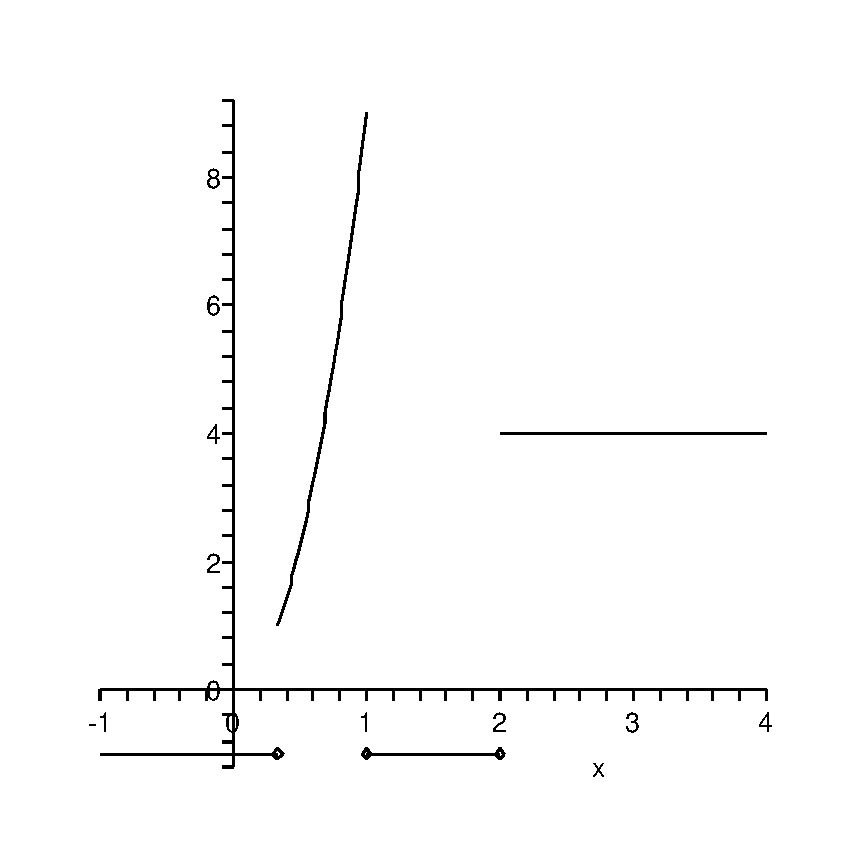
\includegraphics{zzzgraph}} \qedhere \]
 \end{figure}
\end{prf}

\begin{prf}\label{sol_prop_assoc_comp}(Solution to~\ref{prop_assoc_comp})
Associativity: for every $x$
 \[ (h \circ (g \circ f))(x) = h((g \circ f)(x)) = h(g(f(x)))=
              (h \circ g)(f(x)) = ((h \circ g) \circ f)(x)\,; \]
so $h \circ (g \circ f) = (h \circ g) \circ f$.

To see that composition is not commutative take, for example, $f(x) = x + 1$ and $g(x) = x^2$.
Since $(g \circ f)(1) = 4$ and $(f \circ g)(1) = 2$, the functions $g \circ f$ and $f \circ g$
cannot be equal.
\end{prf}






%END appendix L



















\section{Exercises in appendix M}

\begin{prf}\label{sol_exam_inj_fcn}(Solution to~\ref{exam_inj_fcn})
If $f(x) = f(y)$, then $(x + 2)(3y - 5) = (y + 2)(3x - 5)$. Thus $6y - 5x = 6x - 5y$, which
implies $x = y$.
\end{prf}

\begin{prf}\label{sol_exer_inj_q}(Solution to~\ref{exer_inj_q})
Suppose that $m$ and $n$ are positive integers with no common prime factors. Let $f\bigl(\frac
mn\bigr) = 2^m3^n$. Then  $f$ is injective by the \emph{unique factorization theorem} (see,
for example, \cite{BirkhoffMacL:1953}, page~21).
\end{prf}

\begin{prf}\label{sol_exer_surj}(Solution to~\ref{exer_surj})
Let $f(x) = \frac1x - 1$ for $x \ne 0$ and $f(0)~=~3$.
\end{prf}

\begin{prf}\label{sol_exer_bij1}(Solution to~\ref{exer_bij1})
Define $f\colon \Z \sto \N$ by
    \[f(n) = \begin{cases} 2n + 1, &\text{for $n \ge 0$} \\
                             -2n,  &\text{for $n < 0$}.
             \end{cases}   \qedhere \]
\end{prf}

\begin{prf}\label{sol_exer_bij2}(Solution to~\ref{exer_bij2})
Define $f\colon \R \sto (0,1)$ by $f(x) = \frac12 + \frac1\pi \arctan x$.
\end{prf}

\begin{prf}\label{sol_exer_bij3}(Solution to~\ref{exer_bij3})
Let $\Sp^1$ be $\{(x,y)\colon  x^2 + y^2 = 1\}$.  Define $f\colon [0,1) \sto \Sp^1$ by $f(t) =
(\cos(2\pi t), \sin (2\pi t))$.
\end{prf}

\begin{prf}\label{sol_exer_bij4}(Solution to~\ref{exer_bij4})
Let
   \[g(x) = \begin{cases}   3 - 2x,   &\text{for $0 \le x < 1$} \\
                          f(x),       &\text{for $1 \le x \le 2$}\\
                        \frac12(3-x), &\text{for $2 < x \le 3$}.
            \end{cases}   \qedhere\]
\end{prf}

\begin{prf}\label{sol_exer_bij5}(Solution to~\ref{exer_bij5})
$\bigl[-\frac\pi2, \frac\pi2\bigr]$.
\end{prf}

\begin{prf}\label{sol_prop_f_finv}(Solution to~\ref{prop_f_finv})

(a) We show that if $y \in f^{\sto}(f^\gets(B))$, then $y \in B$.  Suppose that $y \in
f^{\sto}(f^\gets(B))$. Then (by the definition of $f^{\sto}$) there exists $x \in f^\gets(B)$
such that $y = f(x)$. From $x \in f^\gets(B)$ we infer (using the definition of $f^\gets$)
that $f(x) \in B$. That is, $y \in B$.

(b) Let $f(x) = x^2$ and $B = \{-1\}$. Then $f^{\sto}(f^\gets(B)) = f^{\sto}(f^\gets\{-1\}) =
f^{\sto}(\emptyset) = \emptyset \ne~B$.

(c) Suppose that $f$ is surjective. Show that $ B \subseteq f^{\sto}(f^\gets(B))$ by showing
that $y \in B$ implies $y \in f^{\sto}(f^\gets(B))$.  If $y \in B$, then (since $f$ is
surjective) there exists $x \in S$ such that $y = f(x)$. Since $f(x) \in B$, we see that $x
\in f^\gets(B)$ (by the definition of $f^\gets$).  From this it follows (using the definition
of $f^{\sto}$) that $y = f(x) \in f^{\sto}(f^\gets(B))$. \qedhere
\end{prf}

\begin{prf}\label{sol_prop_f_union}(Solution to~\ref{prop_f_union})
This requires nothing other than the definitions of $\cup$ and $f^{\sto}$:
 \begin{align*}
   y \in f^{\sto}(A \cup B)
   &\text{ iff there exists $x \in A \cup B$ such that $y=f(x)$}\\
   &\text{ iff there exists $x \in A$ such that $y = f(x)$ or} \\
   &\qquad\text{ there exists $x \in B$ such that $y = f(x)$} \\
   &\text{ iff $y \in f^{\sto}(A)$ or $y \in f^{\sto}(B)$} \\
   &\text{ iff $y \in f^{\sto}(A) \cup f^{\sto}(B)$.}  \qedhere
   \end{align*}
\end{prf}

\begin{prf}\label{sol_prop_finv_intrs}(Solution to~\ref{prop_finv_intrs})
Here the definitions of $\cap$ and $f^\gets$ are used:
\begin{align*}
   x \in f^\gets(C \cap D)
   &\text{ iff $f(x) \in C \cap D$} \\
   &\text{ iff $f(x) \in C$ and $f(x) \in D$} \\
   &\text{ iff $x \in f^\gets(C)$ and $x \in f^\gets(D)$} \\
   &\text{ iff $x \in f^\gets(C) \cap f^\gets(D)$.}  \qedhere
\end{align*}
\end{prf}

\begin{prf}\label{sol_prop_f_fam}(Solution to~\ref{prop_f_fam})

(a) Show that if $y \in f^{\sto}(\bigcap \sfml A)$, then $y \in \bigcap\{f^{\sto}(A)
\colon A \in \sfml A\}$.  Suppose that $y \in f^{\sto}(\bigcap \sfml A)$. Then there
exists $x \in \bigcap\sfml A$ such that $y = f(x)$. Since $x$ belongs to the intersection
of the family $\sfml A$ it must belong to every member of $\sfml A$. That is, $x \in A$
for every $A \in \sfml A$. Thus $y = f(x)$ belongs to $f^{\sto}(A)$ for every $A \in
\sfml A$; and so $y \in \bigcap\{f^{\sto}(A)\colon A \in \sfml A\}$.

(b) Suppose $f$ is injective. If $y \in \bigcap\{f^{\sto}(A)\colon A \in \sfml A\}$, then
$y \in f^{\sto}(A)$ for every $A \in \sfml A$. Choose a set $A_0 \in \sfml A$. Since $y
\in f^{\sto}(A_0)$, there exists $x_0 \in A_0$ such that $y = f(x_0)$. The point $x_0$
belongs to every member of $\sfml A$. To see this, let $A$ be an arbitrary set belonging
to $\sfml A$. Since $y \in f^{\sto}(A)$, there exists $x \in A$ such that $y = f(x)$; and
since $f(x) = y = f(x_0)$ and $f$ is injective, we conclude that $x_0 = x \in A$. Thus we
have shown that $x_0 \in \bigcap\sfml A$ and therefore that $y = f(x_0) \in
f^{\sto}(\bigcap\sfml A)$.

(c) If $y \in f^{\sto}(\bigcup\sfml A)$, then there exists $x \in \bigcup\sfml A$ such
that $y = f(x)$. Since $x \in \bigcup\sfml A$ there exists $A \in \sfml A$ such that $x
\in A$. Then $y = f(x) \in f^{\sto}(A)$ and so $y \in \bigcup\{f^{\sto}(A): A \in \sfml
A\}$. Conversely, if $y$ belongs to $\bigcup\{f^{\sto}(A): A \in \sfml A\}$, then it must
be a member of $f^{\sto}(A)$ for some $A \in \sfml A$. Then $y = f(x)$ for some $x \in A
\subseteq \bigcup\sfml A$ and therefore $y = f(x) \in f^{\sto}(\bigcup\sfml A)$. \qedhere
\end{prf}



\begin{prf}\label{sol_prop_finv_unique}(Solution to~\ref{prop_finv_unique})
Let $f\colon S \sto T$ and suppose that $g$ and $h$ are inverses of $f$. Then
  \[ g = g \circ I_T = g \circ (f \circ h) = (g \circ f) \circ h = I_S
                 \circ h = h\,.\qedhere \]
\end{prf}

\begin{prf}\label{sol_exer_inv_trig}(Solution to~\ref{exer_inv_trig})
\emph{Arcsine} is the inverse of the restriction of the \emph{sine} function to the interval
$[-\frac\pi2,\frac\pi2]$.  The \emph{arccosine} is the inverse of the restriction of
\emph{cosine} to $[0,\pi]$.  And \emph{arctangent} is the inverse of the restriction of
\emph{tangent} to $(-\frac\pi2,\frac\pi2)$.
\end{prf}

\begin{prf}\label{sol_prop_rinv_surj}(Solution to~\ref{prop_rinv_surj})
Suppose that $f$ has a right inverse~$f_r$. For each $y \in T$ it is clear that $y = I_T(y) =
f\bigl(f_r(y)\bigr) \in \ran f$; so $\ran f = T$ and $f$ is surjective.

Conversely, suppose that $f$ is surjective. Then for every $y \in T$ the set
$f^{\gets}(\{y\})$ is nonempty. For each $y \in T$ let $x_y$ be a member of $f^{\gets}(\{y\})$
and define
 \[ f_r\colon T \sto S\colon y \mapsto x_y\,. \]
Then $f\bigl(f_r(y)\bigr) = f(x_y) = y$, showing that $f_r$ is a right inverse of~$f$.
(The reader who has studied a bit of set theory will likely have noticed the unadvertised
use of the
 \index{axiom!of choice}%
 \index{choice, axiom of}%
\emph{axiom of choice} in this proof. It is used in this fashion throughout the text.)
\end{prf}






%END appendix M
















\section{Exercises in appendix N}

\begin{prf}\label{sol_prod_exer}(Solution to~\ref{prod_exer})
The existence of the function has already been demonstrated: if $f = (f^1,f^2)$, then $(\pi_k
\circ f)(t) = \pi_k\bigl(f^1(t),f^2(t)\bigr) = f^k(t)$ for $k = 1,2$ and $t \in T$.

To prove uniqueness suppose that there is a function $g \in \fml F(T,S_1 \times S_2)$ such
that $\pi_k \circ g = f^k$ for $k = 1,2$. Then $g(t) = \bigl(\pi_1(g(t)), \pi_2(g(t))\bigr) =
\bigl(f^1(t),f^2(t)\bigr) = \bigl(f^1,f^2\bigr)(t)$ for $k = 1,2$ and $t \in T$.  So $g =
\bigl(f^1,f^2\bigr)$.
\end{prf}





%END appendix N




















\section{Exercises in appendix O}

\begin{prf}\label{sol_prop_card_n}(Solution to~\ref{prop_card_n})
We wish to demonstrate that for all natural numbers $m$ and $n$ if there is a bijection from
$\{1,\dots, m\}$ onto $\{1,\dots, n\}$, then $m = n$.  To accomplish this use induction
on~$n$.

First, suppose that for an arbitrary natural number $m$ we have $\{1,\dots, m\} \sim \{1\}$.
That is, we suppose that there exists a bijection $f$ from $\{1, \dots, m\}$ onto $\{1\}$.
Then since $f(1) = 1 = f(m)$ and $f$ is injective, we conclude that $m = 1$. This establishes
the proposition in the case $n = 1$.

Next, we assume the truth of the result for some particular $n \in \N$: for every $m \in \N$
if $\{1,\dots, m\} \sim \{1,\dots, n\}$, then $m = n$.  This is our inductive hypothesis. What
we wish to show is that for an arbitrary natural number $m$ if $\{1,\dots, m\} \sim \{1,\dots,
n+1\}$, then $m = n+1$.  Suppose then that $m \in \N$ and $\{1,\dots, m\} \sim
\{1,\dots,n+1\}$. Then there is a bijection $f$ from $\{1,\dots,m\}$ onto $\{1,\dots,n + 1\}$.
Let $k = f^{-1}(n + 1)$. The restriction of $f$ to the set $\{1,\dots,k - 1,k~+~1~, \dots,m\}$
is a bijection from that set onto $\{1,\dots,n\}$. Thus
  \begin{equation}\label{eqn_card_n1}
         \{1,\dots,k - 1,k + 1,\dots,m\} \sim \{1,\dots,n\}.
  \end{equation}
Furthermore, it is easy to see that
  \begin{equation}\label{eqn_card_n2}
         \{1,\dots,m - 1\} \sim \{1,\dots,k - 1,k + 1,\dots,m\}.
  \end{equation}
(The required bijection is defined by $g(j) = j$ if $1 \le j \le k - 1$ and $g(j) = j + 1$ if
$k \le j \le m - 1$.) From \eqref{eqn_card_n1}, \eqref{eqn_card_n2}, and
proposition~\ref{prop_ce_er} we conclude that
  \[ \{1,\dots,m-1\} \sim \{1,\dots,n\}\,. \]
By our inductive hypothesis, $m - 1 = n$. This yields the desired conclusion $m = n + 1$.
\end{prf}

\begin{prf}\label{sol_prop_card_union}(Solution to~\ref{prop_card_union})
The result is trivial if $S$ or $T$ is empty; so we suppose they are not. Let $m = \card S$
and $n = \card T$.  Then $S \sim \{1,\dots,m\}$ and $T \sim \{1,\dots,n\}$. It is clear that
  \[ \{1,\dots,n\} \sim \{m+1,\dots,m + n\}\,. \]
(Use the map $j \mapsto j + m$ for $1 \le j \le n$.)  Thus $T \sim \{m + 1,\dots,m + n\}$. Let
$f \colon S \sto \{1,\dots,m\}$ and $g \colon T \sto \{m + 1,\dots,m + n\}$ be bijections.
Define $h \colon S \cup T \sto \{1,\dots,m + n\}$ by
  \[h(x) = \begin{cases}
              f(x), &\text{for $x \in S$}\\
              g(x), &\text{for $x \in T$.}
           \end{cases} \]
Then clearly $h$ is a bijection.  So $S \cup T$ is finite and $\card(S \cup T) = m + n = \card S + \card T$.
\end{prf}

\begin{prf}\label{sol_lem_card_sub}(Solution to~\ref{lem_card_sub})
Proceed by mathematical induction. If $C \subseteq \{1\}$, then either $C = \emptyset$, in
which case $\card C = 0$, or else $C = \{1\}$, in which case $\card C = 1$. Thus the lemma is
true if $n = 1$.

Suppose then that the lemma holds for some particular $n \in \N$. We prove its correctness for
$n + 1$. So we assume that $C \subseteq \{1,\dots,n + 1\}$ and prove that $C$ is finite and
that $\card C \le n + 1$.  It is clear that $C \setminus \{n + 1\} \subseteq \{1,\dots,n\}$.
By the inductive hypothesis $C \setminus \{n + 1\}$ is finite and $\card(C \setminus \{n +
1\}) \le n$.  There are two possibilities: $n + 1 \notin C$ and $n + 1 \in C$. In case $n + 1$
does not belong to $C$, then $C = C \setminus \{n + 1\}$; so $C$ is finite and $\card C \le n
< n + 1$.  In the other case, where $n + 1$ does belong to $C$, it is clear that $C$ is finite
(because $C \setminus \{n + 1\}$ is) and we have (by proposition~\ref{prop_card_union})
  \begin{align*}
       \card C  &= \card\bigl((C \setminus \{n + 1\}) \cup \{n + 1\}\bigr) \\
                &= \card(C \setminus \{n + 1\}) + \card(\{n + 1\}) \\
                &\le n + 1.        \qedhere
  \end{align*}
\end{prf}

\begin{prf}\label{sol_prop_ce_sub}(Solution to~\ref{prop_ce_sub})
Suppose that $S$ is infinite.  We prove that there exists a proper subset $T$ of $S$ and a
bijection $f$ from $S$ onto $T$. We choose a sequence of distinct elements $a_k$ in $S$, one
for each $k \in \N$. Let $a_1$ be an arbitrary member of $S$. Then $S \setminus \{a_1\} \ne
\emptyset$. (Otherwise $S \sim \{a_1\}$ and $S$ is finite.) Choose $a_2 \in S \setminus
\{a_1\}$. Then $S \setminus \{a_1,a_2\} \ne \emptyset$. (Otherwise $S \sim \{a_1,a_2\}$ and
$S$ is finite.) In general, if distinct elements $a_1,\dots,a_n$ have been chosen, then $S
\setminus \{a_1,\dots,a_n\}$ cannot be empty; so we may choose $a_{n+1} \in S \setminus
\{a_1,\dots,a_n\}$. Let $T = S \setminus \{a_1\}$, and define $f \colon S \sto T$ by
   \[f(x) = \begin{cases}
                 a_{k+1}, &\text{if $x=a_k$ for some $k$}\\
                 x,       &\text{otherwise}.
            \end{cases}\]
Then $f$ is a bijection from $S$ onto the proper subset $T$ of~$S$.

For the converse construct a proof by contradiction. Suppose that $S \sim T$ for some proper
subset $T \subseteq S$, and assume further that $S$ is finite, so that $S \sim \{1,\dots,n\}$
for some $n \in \N$. Then by proposition \ref{prop_card_sub} the set $S \setminus T$ is finite
and, since it is nonempty, is therefore cardinally equivalent to $\{1,\dots,p\}$ for some $p
\in \N$. Thus
  \begin{align*}
       n &= \card S\\
         &= \card T\\
         &= \card (S \setminus (S \setminus T))\\
         &= \card S - \card(S \setminus T)\qquad \text{(by problem \ref{prob_card_diff})} \\
         &= n - p.
  \end{align*}
Therefore $p = 0$, which contradicts the earlier assertion that $p \in \N$.
\end{prf}

\begin{prf}\label{sol_exer_int_inf}(Solution to~\ref{exer_int_inf})
The map $x \mapsto \frac12x$ is a bijection from the interval $(0,1)$ onto the interval
$(0,\frac12)$, which is a proper subset of~$(0,1)$.
\end{prf}

\begin{prf}\label{sol_prop_ran_fin}(Solution to~\ref{prop_ran_fin})
Since $f$ is surjective it has a right inverse $f_r$ (see proposition \ref{prop_rinv_surj}).
This right inverse is injective, since it has a left inverse (see
proposition~\ref{prop_linv_inj}). Let $A = \ran f_r$. The function $f_r$ establishes a
bijection between $T$ and~$A$. Thus $T \sim A \subseteq S$. If $S$ is finite, so is $A$ (by
proposition \ref{prop_card_sub}) and therefore so is $T$.
\end{prf}

\begin{prf}\label{sol_prop_preimg_fin}(Solution to~\ref{prop_preimg_fin})
Let $B = \ran f$. Then $S \sim B \subseteq T$. If $T$ is finite, so is $B$ (by
proposition~\ref{prop_card_sub}) and therefore so is~$S$.
\end{prf}





%END appendix O















\section{Exercises in appendix P}

\begin{prf}\label{sol_prop_sub_cntbl}(Solution to~\ref{prop_sub_cntbl})
If $S$ is finite there is nothing to prove; so we suppose that $S$ is an infinite subset of
$T$.  Then $T$ is countably infinite.  Let $f \colon \N \sto T$ be an enumeration of the
members of $T$. The restriction of $f$ to the set $f^\gets(S) \subseteq \N$ is a bijection
between $f^\gets(S)$ and $S$; so we may conclude that $S$ is countable provided we can prove
that $f^\gets(S)$ is. Therefore it suffices to show that \emph{every} subset of $\N$  is
countable.

Let $A$ be an infinite subset of $\N$. Define inductively elements $a_1 < a_2 < \dots$ in $A$.
(Let $a_1$ be the smallest member of $A$. Having chosen $a_1 < a_2 < \dots < a_n$ in $A$,
notice that the set $A \setminus \{a_1,\dots,a_n\}$ is not empty and choose $a_{n+1}$ to be
the smallest element of that set.)  Let $a \colon \N \sto A$ be the function $n \mapsto a_n$.
It is clear that $a_k \ge k$ for all $k$ and, since $a_k < a_{k+1}$ for all $k$, that $a$ is
injective.  To see that $a$ is surjective, assume that it is not and derive a contradiction.
If $a$ is not surjective, then the range of $a$ is a proper subset of $A$.  Let $p$ be the
smallest element of $A \setminus \ran a$.  Since $p \in A \setminus \ran a \subseteq A
\setminus \{a_1,\dots,a_p\}$, we see from the definition of $a_{p+1}$ that $a_{p+1} \le p$. On
the other hand we know that $ a_{p+1} \ge p + 1 > p$.  This contradiction shows that $a$ is a
surjection.  Thus $A \sim \N$ proving that $A$ is countable.
\end{prf}

\begin{prf}\label{sol_lem_nxn_cntbl}(Solution to~\ref{lem_nxn_cntbl})
To see that the map
  \[ f \colon \N \times \N \sto \N \colon (m,n) \mapsto 2^{m-1}(2n - 1) \]
is a bijection, we construct its inverse (see propositions \ref{prop_rinv_surj}
and~\ref{prop_linv_inj}).  If $p \in \N$ let $m$ be the largest member of $\N$ such that
$2^{m-1}$ divides $p$. (If $p$ is odd, then $m=1$.) Then $p/2^{m-1}$ is odd and can be written
in the form $2n-1$ for some $n \in \N$. The map $g \colon p \mapsto (m,n)$ is clearly the
inverse of~$f$.
\end{prf}

\begin{prf}\label{sol_prop_union_cntbl}(Solution to~\ref{prop_union_cntbl})
If $\sfml A$ is infinite let
  \[ \sfml A = \{A_1,A_2,A_3, \dots\}\,; \]
while if $\sfml A$ is finite, say $\card\sfml A = m$, let
  \[ \sfml A = \{A_1, \dots,A_m\} \]
and let $A_n = A_m$ for all $n > m$.  For each $j \in \N$ the set $A_j$ is either infinite, in
which case we write
  \[ A_j = \{a_{j1},a_{j2}, a_{j3},\dots\}\,, \]
or else it is finite, say $\card A_j = p$, in which case we write
  \[ A_j = \{a_{j1},\dots,a_{jp}\} \]
and let $a_{jq} = a_{jp}$ for all $q > p$.  Then the map
  \[a \colon \N \times \N \sto \bigcup\sfml A \colon (j,k) \mapsto a_{jk} \]
is surjective.  Thus $\bigcup\sfml A = \bigcup\limits_{j,k=1}^\infty A_{j,k} = \ran a$ is
countable by lemma~\ref{lem_nxn_cntbl} and proposition~\ref{prop_ran_cntbl}.
\end{prf}





\endinput


\backmatter


 \cleardoublepage
 \phantomsection
        %allows TOC links to find bibliography correctly
 \bibliographystyle{plain}
 \bibliography{probtextbib}
 %\addcontentsline{toc}{chapter}{Bibliography}


 \cleardoublepage
 \phantomsection
         %allows TOC links to find index correctly
 \printindex
 \addcontentsline{toc}{chapter}{Index}



\end{document}
